\chapter{Tree-structure segmentation for logistic regression} \label{chap6}

\selectlanguage{english}

\epigraph{All religions, arts and sciences are branches of the same tree. All these aspirations are directed toward ennobling man's life, lifting it from the sphere of mere physical existence and leading the individual towards freedom.}{Albert Einstein, ``Moral Decay'', 1937.}

\minitoc

\bigskip

In Chapter~\ref{chap1}, it was argued in Section~\ref{subsec:segmentation} that, what is referred to as ``segmentation'' in the \textit{Credit Scoring} industry, could be a straightforward solution to deal with missing values and outliers that are quite common problems in \textit{Credit Scoring}. This means we learn ``expert'' \gls{lr} models on separate ``segments'' of clients arranged in a tree. Its more theoretical justification is similar to that of quantization, sketched in Section~\ref{sec:bias_variance_quant}, which is to achieve a good bias-variance trade-off of the predictive task. This goal was embedded explicitly in the proposed quantization algorithm. Here again, the resulting segmentation and scorecards therein can be viewed as a single model for the whole population. In the next section, we give some industrial context to the problem which is followed in Section~\ref{sec:literature} by a literature review. Section~\ref{sec:model_selec_tree} reinterprets this problem, as advertised, as a model selection problem for which a specific approach is designed in subsequent sections.


\section{Introduction}

\subsection{Context} \label{subsec:context}

As was emphasized in all previous chapters, \gls{lr} is the building block of a scorecard predicting the creditworthiness of an applicant and partly automating the acceptance / rejection mechanism. However, estimating \gls{lr} coefficients means that training data $(\gls{bbx},\gls{bby})$ is available. This is not the case when a new product, \textit{e.g.}\ smartphone leasing, is added to the acceptance system. On a practical note, some other previously learnt scorecard may not be applicable on this new market because the same information is not asked to applicants, \textit{e.g.}\ marital status, because given the low amounts at stake, it was decided to collect the fewest data possible, to make the process as simple and quick as possible. On a more theoretical note, it is probable that applicants to smartphone leasing are not stemming from the same data generating mechanism $\gls{bX},\gls{Y} \sim p$ as any other previous applicants (\textit{i.e.}\ on other markets). Put it another way, the possibility of having several \gls{lr} scorecards on sub-populations of the total portfolio allows to have more flexibility, and thus it potentially reduces model bias discussed in Chapter~\ref{chap1}.

For these reasons, several industries, among which \textit{Credit Scoring}, rely on several ``weak learners'' such as \gls{lr}, arranged in a tree. Such decision process is illustrated on Figure~\ref{fig:arbre}. This tree structure and the vocabulary of ``weak learners'' would indicate a use-case of Mixtures of Experts~\cite{jordan1994hierarchical} or aggregation / ensemble methods~\cite{opitz1999popular} respectively. However, these fuzzy methods imply that all applicants are scored by all scorecards, which is obviously neither desirable (for interpretation purposes) nor feasible (since available features differ).

The next section illustrates how such a structure is achieved using \gls{cacf}'s in-house practices.

\tikzstyle{level 1}=[level distance=2.2cm, sibling distance=7cm]
\tikzstyle{level 2}=[level distance=2cm, sibling distance=5cm]
\tikzstyle{level 3}=[level distance=2cm, sibling distance=3cm]

\begin{figure}
\resizebox{\textwidth}{!}{
\centering
\begin{tikzpicture}
  [
    sibling distance        = 15em,
    level distance          = 5em,
    edge from parent/.style = {draw, -latex},
    every node/.style       = {font=\footnotesize},
    sloped
  ]
  \node [root] {\textcolor{black}{Applicants}}
    child { node [dummy] {}
      child { node [dummy] {}
        child { node [env] {\textcolor{black}{$p_{\gls{bth}^1}(y|\q^1(\gls{bx}),\bdelta^1)$ \hspace*{-0.4cm}}}
          edge from parent node [below] {Renters} }
        child { node [env] {\textcolor{black}{$p_{\gls{bth}^2}(y|\q^2(\gls{bx}),\bdelta^2)$ \hspace*{-0.4cm}}}
          edge from parent node [above] {Salaried} }
        child { node [env] {\textcolor{black}{$p_{\gls{bth}^3}(y|\q^3(\gls{bx}),\bdelta^3)$ \hspace*{-0.4cm}}}
                edge from parent node [above] {Others} }
        edge from parent node [above] {Revolving} }
      child { node [env] {\textcolor{black}{$p_{\gls{bth}^4}(y|\q^4(\gls{bx}),\bdelta^4)$ \hspace*{-0.4cm}}}
              edge from parent node [above, align=center]
                {Standard loan} }
              edge from parent node [above] {Home Appliances} }
    child { node [dummy] {}
      child { node [dummy] {}
        child { node [env] {\textcolor{black}{$p_{\gls{bth}^5}(y|\q^5(\gls{bx}),\bdelta^5)$ \hspace*{-0.4cm}}}
          edge from parent node [above] {Leasing} }
        child { node [env] {\textcolor{black}{$p_{\gls{bth}^6}(y|\q^6(\gls{bx}),\bdelta^6)$ \hspace*{-0.4cm}}}
                edge from parent node [above] {Standard loan} }
        edge from parent node [above] {Fiat} }
      child { node [env] {\textcolor{black}{$p_{\gls{bth}^7}(y|\q^7(\gls{bx}),\bdelta^7)$ \hspace*{-0.4cm}}}
              edge from parent node [above, align=center]
                {Kawasaki} }
              edge from parent node [above] {Automobile} };
\end{tikzpicture}
}
\caption{Simplified cartography of the application scorecards.}
\label{fig:arbre}
\end{figure}




\subsection{In-house \textit{ad hoc} practice} \label{subsec:adhoc}

\textit{Credit Scoring} practitioners are often asked by the management to ``locally'' study the decision process displayed on Figure~\ref{fig:arbre} by \textit{e.g.}\ merging branches (Standard loans and Leasing for Fiat) or conversely to separate sub-populations by splitting a leaf (Kawasaki into Standard loans and Leasing). To do so, they resort to simple unsupervised generative clustering techniques, such as \gls{pca} and its refinements on categorical or mixed data (\gls{mca} or \gls{famd} resp.) which are described hereafter.

\paragraph{\glsfirst{pca}}

The goal of \gls{pca}~\cite{pages2014multiple} is to represent observations graphically in a way that exhibits most efficiently their similitude and differences by combining input features in so-called orthogonal ``principal components'' $\bm{u} = (\bm{u}_1,\dots,\bm{u}_d)$ such that the inertia of each axis $j$ (the variance of $\gls{bx}' \bm{u}_j$) is maximized. It can be shown that it is equivalent to seeking the ordering of the eigenvalues $\bm{\lambda} = (\lambda_1,\dots,\lambda_d)$ of the covariance matrix $\Sigma = \gls{bbx}'\gls{bbx}$. The explained variance of each axis $j$ is given by $\frac{\lambda_j}{\sum_{j'=1}^d \lambda_j'}$. Classically, only the two first axes $(\bm{u}_1,\bm{u}_2)$ (after reordering from largest to lowest explained variance) are used. The composition of theses axes in the original features $\gls{x}_j$ is often represented first, to see if groups of features can be formed which would define the subsequent segments. \gls{pca} has been applied to the Automobile dataset from \gls{cacf} ($n = 50{,}000$, $d = 25$ among which $18$ continuous and $7$ categorical features which number of levels go from $5$ - family status - to $100$ - brand of the vehicle and $200{,}000$ missing entries) on Figure~\ref{fig:pca}, where the aforementioned principal components' composition is displayed on Figure~\ref{fig:pca1}: interestingly, the first axis is dominated by car and loan characteristics such as the vehicle's price (``APPORT'', ``MCDE'', ``CREDAC''), its fiscal and mechanical characteristics (``CVFISC'', ``POIDSVH'', ``CYLVH'') while the second axis is composed of clients' characteristics such as their age (``anc\_DNAISS'', ``anc\_DNACJ''), their number of children (``NBENF''), their job stability (``anc\_AMEMBC''). Note that a good portion of the total variance is explained by the first axes (22.54 \% and 18.97 \% resp.). The second classical representation is the observations themselves in this new space, which is displayed on Figure~\ref{fig:pca2}: no clear group is distinguishable from the pack. With these two representations, the \textit{Credit Scoring} practitioner decide if, visually, clusters are formed (\textit{i.e.}\ clouds with little intra-class variance) which would be used to build separate scorecards $(p_{\gls{bth}^{1}},p_{\gls{bth}^{2}})$.
%The method is described in Appendix~\ref{app1:pca}.

However, the \textit{Credit Scoring} data is of mixed type and \textit{Credit Scoring} practitioners are used to quantizing the data, as explained thoroughly in Chapter~\ref{chap4}, such that the \gls{mca} algorithm, specific to categorical features, becomes applicable to all features, by using \textit{e.g.\ equal-freq} or $\chi^2$ tests (see Appendix~\ref{app1}).

\begin{figure}[!htb]
{\setlength{\parindent}{0cm}}
\begin{multicols}{2}
\centering
\begin{subfigure}[t]{0.45\textwidth}
\centering
\resizebox{\textwidth}{!}{% Created by tikzDevice version 0.12 on 2019-03-01 10:28:44
% !TEX encoding = UTF-8 Unicode
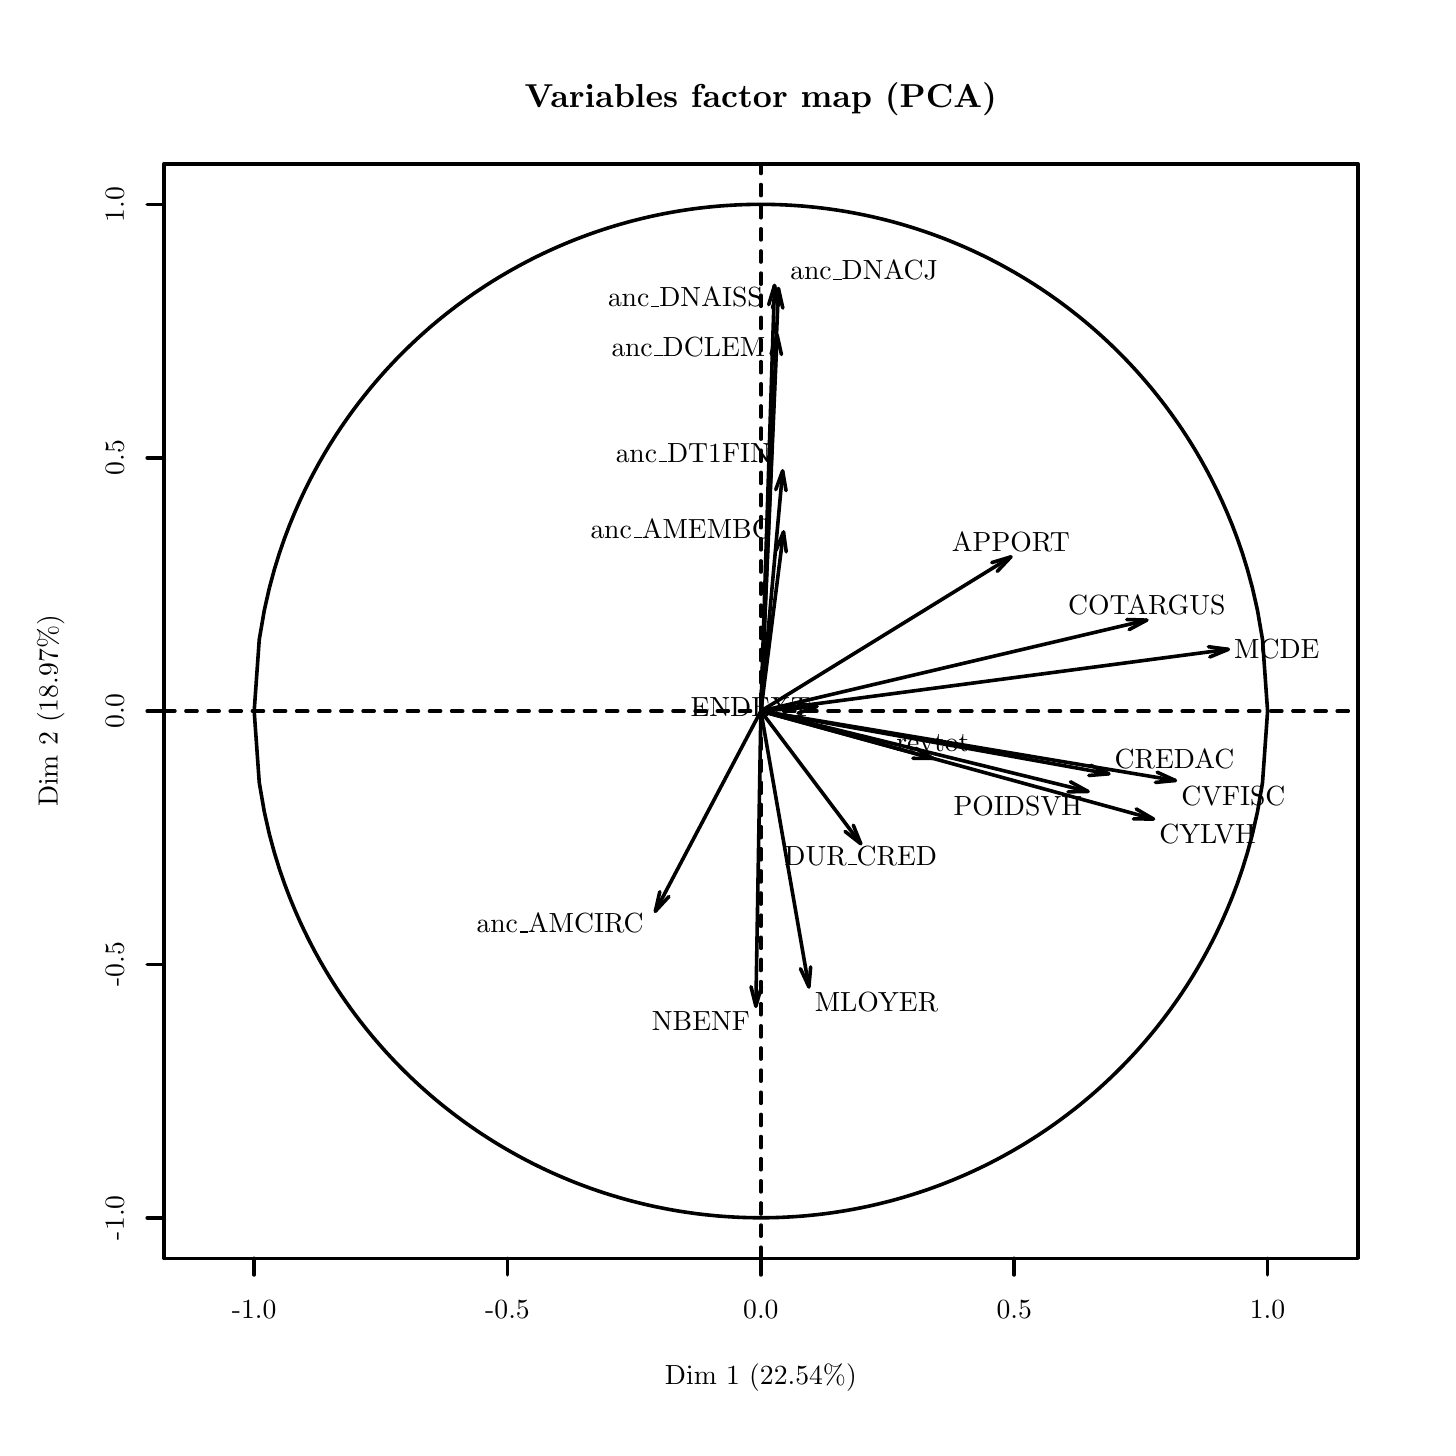
\begin{tikzpicture}[x=1pt,y=1pt]
\definecolor{fillColor}{RGB}{255,255,255}
\path[use as bounding box,fill=fillColor,fill opacity=0.00] (0,0) rectangle (505.89,505.89);
\begin{scope}
\path[clip] ( 49.20, 61.20) rectangle (480.69,456.69);
\definecolor{drawColor}{RGB}{255,255,255}

\path[draw=drawColor,line width= 1.3pt,line join=round,line cap=round] (264.94,258.94) circle (  2.25);
\end{scope}
\begin{scope}
\path[clip] (  0.00,  0.00) rectangle (505.89,505.89);
\definecolor{drawColor}{RGB}{0,0,0}

\path[draw=drawColor,line width= 1.3pt,line join=round,line cap=round] ( 81.85, 61.20) -- (448.04, 61.20);

\path[draw=drawColor,line width= 1.3pt,line join=round,line cap=round] ( 81.85, 61.20) -- ( 81.85, 55.20);

\path[draw=drawColor,line width= 1.3pt,line join=round,line cap=round] (173.40, 61.20) -- (173.40, 55.20);

\path[draw=drawColor,line width= 1.3pt,line join=round,line cap=round] (264.94, 61.20) -- (264.94, 55.20);

\path[draw=drawColor,line width= 1.3pt,line join=round,line cap=round] (356.49, 61.20) -- (356.49, 55.20);

\path[draw=drawColor,line width= 1.3pt,line join=round,line cap=round] (448.04, 61.20) -- (448.04, 55.20);

\node[text=drawColor,anchor=base,inner sep=0pt, outer sep=0pt, scale=  1.00] at ( 81.85, 39.60) {-1.0};

\node[text=drawColor,anchor=base,inner sep=0pt, outer sep=0pt, scale=  1.00] at (173.40, 39.60) {-0.5};

\node[text=drawColor,anchor=base,inner sep=0pt, outer sep=0pt, scale=  1.00] at (264.94, 39.60) {0.0};

\node[text=drawColor,anchor=base,inner sep=0pt, outer sep=0pt, scale=  1.00] at (356.49, 39.60) {0.5};

\node[text=drawColor,anchor=base,inner sep=0pt, outer sep=0pt, scale=  1.00] at (448.04, 39.60) {1.0};

\path[draw=drawColor,line width= 1.3pt,line join=round,line cap=round] ( 49.20, 75.85) -- ( 49.20,442.04);

\path[draw=drawColor,line width= 1.3pt,line join=round,line cap=round] ( 49.20, 75.85) -- ( 43.20, 75.85);

\path[draw=drawColor,line width= 1.3pt,line join=round,line cap=round] ( 49.20,167.40) -- ( 43.20,167.40);

\path[draw=drawColor,line width= 1.3pt,line join=round,line cap=round] ( 49.20,258.94) -- ( 43.20,258.94);

\path[draw=drawColor,line width= 1.3pt,line join=round,line cap=round] ( 49.20,350.49) -- ( 43.20,350.49);

\path[draw=drawColor,line width= 1.3pt,line join=round,line cap=round] ( 49.20,442.04) -- ( 43.20,442.04);

\node[text=drawColor,rotate= 90.00,anchor=base,inner sep=0pt, outer sep=0pt, scale=  1.00] at ( 34.80, 75.85) {-1.0};

\node[text=drawColor,rotate= 90.00,anchor=base,inner sep=0pt, outer sep=0pt, scale=  1.00] at ( 34.80,167.40) {-0.5};

\node[text=drawColor,rotate= 90.00,anchor=base,inner sep=0pt, outer sep=0pt, scale=  1.00] at ( 34.80,258.94) {0.0};

\node[text=drawColor,rotate= 90.00,anchor=base,inner sep=0pt, outer sep=0pt, scale=  1.00] at ( 34.80,350.49) {0.5};

\node[text=drawColor,rotate= 90.00,anchor=base,inner sep=0pt, outer sep=0pt, scale=  1.00] at ( 34.80,442.04) {1.0};

\path[draw=drawColor,line width= 1.3pt,line join=round,line cap=round] ( 49.20, 61.20) --
	(480.69, 61.20) --
	(480.69,456.69) --
	( 49.20,456.69) --
	( 49.20, 61.20);
\end{scope}
\begin{scope}
\path[clip] (  0.00,  0.00) rectangle (505.89,505.89);
\definecolor{drawColor}{RGB}{0,0,0}

\node[text=drawColor,anchor=base,inner sep=0pt, outer sep=0pt, scale=  1.20] at (264.94,477.15) {\bfseries Variables factor map (PCA)};

\node[text=drawColor,anchor=base,inner sep=0pt, outer sep=0pt, scale=  1.00] at (264.94, 15.60) {Dim 1 (22.54{\%})};

\node[text=drawColor,rotate= 90.00,anchor=base,inner sep=0pt, outer sep=0pt, scale=  1.00] at ( 10.80,258.94) {Dim 2 (18.97{\%})};
\end{scope}
\begin{scope}
\path[clip] ( 49.20, 61.20) rectangle (480.69,456.69);
\definecolor{drawColor}{RGB}{0,0,0}

\path[draw=drawColor,line width= 1.3pt,line join=round,line cap=round] ( 81.85,258.94) --
	( 83.68,284.77) --
	( 85.51,295.38) --
	( 87.34,303.46) --
	( 89.17,310.21) --
	( 91.00,316.12) --
	( 92.83,321.41) --
	( 94.66,326.24) --
	( 96.50,330.70) --
	( 98.33,334.86) --
	(100.16,338.76) --
	(101.99,342.43) --
	(103.82,345.91) --
	(105.65,349.22) --
	(107.48,352.38) --
	(109.31,355.40) --
	(111.14,358.29) --
	(112.97,361.07) --
	(114.81,363.74) --
	(116.64,366.32) --
	(118.47,368.80) --
	(120.30,371.20) --
	(122.13,373.52) --
	(123.96,375.77) --
	(125.79,377.94) --
	(127.62,380.05) --
	(129.45,382.10) --
	(131.28,384.08) --
	(133.11,386.01) --
	(134.95,387.88) --
	(136.78,389.70) --
	(138.61,391.47) --
	(140.44,393.19) --
	(142.27,394.87) --
	(144.10,396.50) --
	(145.93,398.09) --
	(147.76,399.63) --
	(149.59,401.14) --
	(151.42,402.60) --
	(153.26,404.03) --
	(155.09,405.42) --
	(156.92,406.78) --
	(158.75,408.10) --
	(160.58,409.39) --
	(162.41,410.64) --
	(164.24,411.86) --
	(166.07,413.05) --
	(167.90,414.21) --
	(169.73,415.34) --
	(171.57,416.44) --
	(173.40,417.51) --
	(175.23,418.55) --
	(177.06,419.57) --
	(178.89,420.56) --
	(180.72,421.52) --
	(182.55,422.46) --
	(184.38,423.37) --
	(186.21,424.25) --
	(188.04,425.11) --
	(189.88,425.95) --
	(191.71,426.76) --
	(193.54,427.54) --
	(195.37,428.31) --
	(197.20,429.05) --
	(199.03,429.77) --
	(200.86,430.46) --
	(202.69,431.13) --
	(204.52,431.79) --
	(206.35,432.41) --
	(208.18,433.02) --
	(210.02,433.61) --
	(211.85,434.17) --
	(213.68,434.72) --
	(215.51,435.24) --
	(217.34,435.75) --
	(219.17,436.23) --
	(221.00,436.69) --
	(222.83,437.13) --
	(224.66,437.56) --
	(226.49,437.96) --
	(228.33,438.34) --
	(230.16,438.71) --
	(231.99,439.05) --
	(233.82,439.38) --
	(235.65,439.68) --
	(237.48,439.97) --
	(239.31,440.24) --
	(241.14,440.49) --
	(242.97,440.72) --
	(244.80,440.93) --
	(246.64,441.12) --
	(248.47,441.30) --
	(250.30,441.46) --
	(252.13,441.59) --
	(253.96,441.71) --
	(255.79,441.81) --
	(257.62,441.90) --
	(259.45,441.96) --
	(261.28,442.01) --
	(263.11,442.03) --
	(264.94,442.04) --
	(266.78,442.03) --
	(268.61,442.01) --
	(270.44,441.96) --
	(272.27,441.90) --
	(274.10,441.81) --
	(275.93,441.71) --
	(277.76,441.59) --
	(279.59,441.46) --
	(281.42,441.30) --
	(283.25,441.12) --
	(285.09,440.93) --
	(286.92,440.72) --
	(288.75,440.49) --
	(290.58,440.24) --
	(292.41,439.97) --
	(294.24,439.68) --
	(296.07,439.38) --
	(297.90,439.05) --
	(299.73,438.71) --
	(301.56,438.34) --
	(303.40,437.96) --
	(305.23,437.56) --
	(307.06,437.13) --
	(308.89,436.69) --
	(310.72,436.23) --
	(312.55,435.75) --
	(314.38,435.24) --
	(316.21,434.72) --
	(318.04,434.17) --
	(319.87,433.61) --
	(321.71,433.02) --
	(323.54,432.41) --
	(325.37,431.79) --
	(327.20,431.13) --
	(329.03,430.46) --
	(330.86,429.77) --
	(332.69,429.05) --
	(334.52,428.31) --
	(336.35,427.54) --
	(338.18,426.76) --
	(340.01,425.95) --
	(341.85,425.11) --
	(343.68,424.25) --
	(345.51,423.37) --
	(347.34,422.46) --
	(349.17,421.52) --
	(351.00,420.56) --
	(352.83,419.57) --
	(354.66,418.55) --
	(356.49,417.51) --
	(358.32,416.44) --
	(360.16,415.34) --
	(361.99,414.21) --
	(363.82,413.05) --
	(365.65,411.86) --
	(367.48,410.64) --
	(369.31,409.39) --
	(371.14,408.10) --
	(372.97,406.78) --
	(374.80,405.42) --
	(376.63,404.03) --
	(378.47,402.60) --
	(380.30,401.14) --
	(382.13,399.63) --
	(383.96,398.09) --
	(385.79,396.50) --
	(387.62,394.87) --
	(389.45,393.19) --
	(391.28,391.47) --
	(393.11,389.70) --
	(394.94,387.88) --
	(396.77,386.01) --
	(398.61,384.08) --
	(400.44,382.10) --
	(402.27,380.05) --
	(404.10,377.94) --
	(405.93,375.77) --
	(407.76,373.52) --
	(409.59,371.20) --
	(411.42,368.80) --
	(413.25,366.32) --
	(415.08,363.74) --
	(416.92,361.07) --
	(418.75,358.29) --
	(420.58,355.40) --
	(422.41,352.38) --
	(424.24,349.22) --
	(426.07,345.91) --
	(427.90,342.43) --
	(429.73,338.76) --
	(431.56,334.86) --
	(433.39,330.70) --
	(435.23,326.24) --
	(437.06,321.41) --
	(438.89,316.12) --
	(440.72,310.21) --
	(442.55,303.46) --
	(444.38,295.38) --
	(446.21,284.77) --
	(448.04,258.94);

\path[draw=drawColor,line width= 1.3pt,line join=round,line cap=round] ( 81.85,258.94) --
	( 83.68,233.12) --
	( 85.51,222.51) --
	( 87.34,214.43) --
	( 89.17,207.68) --
	( 91.00,201.77) --
	( 92.83,196.48) --
	( 94.66,191.65) --
	( 96.50,187.19) --
	( 98.33,183.03) --
	(100.16,179.13) --
	(101.99,175.46) --
	(103.82,171.98) --
	(105.65,168.67) --
	(107.48,165.51) --
	(109.31,162.49) --
	(111.14,159.60) --
	(112.97,156.82) --
	(114.81,154.15) --
	(116.64,151.57) --
	(118.47,149.09) --
	(120.30,146.69) --
	(122.13,144.37) --
	(123.96,142.12) --
	(125.79,139.95) --
	(127.62,137.84) --
	(129.45,135.79) --
	(131.28,133.81) --
	(133.11,131.88) --
	(134.95,130.01) --
	(136.78,128.19) --
	(138.61,126.42) --
	(140.44,124.70) --
	(142.27,123.02) --
	(144.10,121.39) --
	(145.93,119.80) --
	(147.76,118.26) --
	(149.59,116.75) --
	(151.42,115.29) --
	(153.26,113.86) --
	(155.09,112.47) --
	(156.92,111.11) --
	(158.75,109.79) --
	(160.58,108.50) --
	(162.41,107.25) --
	(164.24,106.03) --
	(166.07,104.84) --
	(167.90,103.68) --
	(169.73,102.55) --
	(171.57,101.45) --
	(173.40,100.38) --
	(175.23, 99.34) --
	(177.06, 98.32) --
	(178.89, 97.33) --
	(180.72, 96.37) --
	(182.55, 95.43) --
	(184.38, 94.52) --
	(186.21, 93.64) --
	(188.04, 92.78) --
	(189.88, 91.94) --
	(191.71, 91.13) --
	(193.54, 90.35) --
	(195.37, 89.58) --
	(197.20, 88.84) --
	(199.03, 88.12) --
	(200.86, 87.43) --
	(202.69, 86.76) --
	(204.52, 86.10) --
	(206.35, 85.48) --
	(208.18, 84.87) --
	(210.02, 84.28) --
	(211.85, 83.72) --
	(213.68, 83.17) --
	(215.51, 82.65) --
	(217.34, 82.14) --
	(219.17, 81.66) --
	(221.00, 81.20) --
	(222.83, 80.76) --
	(224.66, 80.33) --
	(226.49, 79.93) --
	(228.33, 79.55) --
	(230.16, 79.18) --
	(231.99, 78.84) --
	(233.82, 78.51) --
	(235.65, 78.21) --
	(237.48, 77.92) --
	(239.31, 77.65) --
	(241.14, 77.40) --
	(242.97, 77.17) --
	(244.80, 76.96) --
	(246.64, 76.77) --
	(248.47, 76.59) --
	(250.30, 76.43) --
	(252.13, 76.30) --
	(253.96, 76.18) --
	(255.79, 76.08) --
	(257.62, 75.99) --
	(259.45, 75.93) --
	(261.28, 75.88) --
	(263.11, 75.86) --
	(264.94, 75.85) --
	(266.78, 75.86) --
	(268.61, 75.88) --
	(270.44, 75.93) --
	(272.27, 75.99) --
	(274.10, 76.08) --
	(275.93, 76.18) --
	(277.76, 76.30) --
	(279.59, 76.43) --
	(281.42, 76.59) --
	(283.25, 76.77) --
	(285.09, 76.96) --
	(286.92, 77.17) --
	(288.75, 77.40) --
	(290.58, 77.65) --
	(292.41, 77.92) --
	(294.24, 78.21) --
	(296.07, 78.51) --
	(297.90, 78.84) --
	(299.73, 79.18) --
	(301.56, 79.55) --
	(303.40, 79.93) --
	(305.23, 80.33) --
	(307.06, 80.76) --
	(308.89, 81.20) --
	(310.72, 81.66) --
	(312.55, 82.14) --
	(314.38, 82.65) --
	(316.21, 83.17) --
	(318.04, 83.72) --
	(319.87, 84.28) --
	(321.71, 84.87) --
	(323.54, 85.48) --
	(325.37, 86.10) --
	(327.20, 86.76) --
	(329.03, 87.43) --
	(330.86, 88.12) --
	(332.69, 88.84) --
	(334.52, 89.58) --
	(336.35, 90.35) --
	(338.18, 91.13) --
	(340.01, 91.94) --
	(341.85, 92.78) --
	(343.68, 93.64) --
	(345.51, 94.52) --
	(347.34, 95.43) --
	(349.17, 96.37) --
	(351.00, 97.33) --
	(352.83, 98.32) --
	(354.66, 99.34) --
	(356.49,100.38) --
	(358.32,101.45) --
	(360.16,102.55) --
	(361.99,103.68) --
	(363.82,104.84) --
	(365.65,106.03) --
	(367.48,107.25) --
	(369.31,108.50) --
	(371.14,109.79) --
	(372.97,111.11) --
	(374.80,112.47) --
	(376.63,113.86) --
	(378.47,115.29) --
	(380.30,116.75) --
	(382.13,118.26) --
	(383.96,119.80) --
	(385.79,121.39) --
	(387.62,123.02) --
	(389.45,124.70) --
	(391.28,126.42) --
	(393.11,128.19) --
	(394.94,130.01) --
	(396.77,131.88) --
	(398.61,133.81) --
	(400.44,135.79) --
	(402.27,137.84) --
	(404.10,139.95) --
	(405.93,142.12) --
	(407.76,144.37) --
	(409.59,146.69) --
	(411.42,149.09) --
	(413.25,151.57) --
	(415.08,154.15) --
	(416.92,156.82) --
	(418.75,159.60) --
	(420.58,162.49) --
	(422.41,165.51) --
	(424.24,168.67) --
	(426.07,171.98) --
	(427.90,175.46) --
	(429.73,179.13) --
	(431.56,183.03) --
	(433.39,187.19) --
	(435.23,191.65) --
	(437.06,196.48) --
	(438.89,201.77) --
	(440.72,207.68) --
	(442.55,214.43) --
	(444.38,222.51) --
	(446.21,233.12) --
	(448.04,258.94);

\path[draw=drawColor,line width= 1.3pt,dash pattern=on 4pt off 4pt ,line join=round,line cap=round] (264.94, 61.20) -- (264.94,456.69);

\path[draw=drawColor,line width= 1.3pt,dash pattern=on 4pt off 4pt ,line join=round,line cap=round] ( 49.20,258.94) -- (480.69,258.94);

\path[draw=drawColor,line width= 1.3pt,line join=round,line cap=round] (264.94,258.94) -- (355.30,314.66);

\path[draw=drawColor,line width= 1.3pt,line join=round,line cap=round] (350.34,309.40) --
	(355.30,314.66) --
	(348.37,312.59);

\path[draw=drawColor,line width= 1.3pt,line join=round,line cap=round] (264.94,258.94) -- (404.38,291.80);

\path[draw=drawColor,line width= 1.3pt,line join=round,line cap=round] (398.02,288.38) --
	(404.38,291.80) --
	(397.16,292.02);

\path[draw=drawColor,line width= 1.3pt,line join=round,line cap=round] (264.94,258.94) -- (390.66,236.27);

\path[draw=drawColor,line width= 1.3pt,line join=round,line cap=round] (383.45,235.66) --
	(390.66,236.27) --
	(384.12,239.35);

\path[draw=drawColor,line width= 1.3pt,line join=round,line cap=round] (264.94,258.94) -- (414.71,233.85);

\path[draw=drawColor,line width= 1.3pt,line join=round,line cap=round] (407.52,233.16) --
	(414.71,233.85) --
	(408.14,236.85);

\path[draw=drawColor,line width= 1.3pt,line join=round,line cap=round] (264.94,258.94) -- (406.79,219.94);

\path[draw=drawColor,line width= 1.3pt,line join=round,line cap=round] (399.56,219.98) --
	(406.79,219.94) --
	(400.55,223.59);

\path[draw=drawColor,line width= 1.3pt,line join=round,line cap=round] (264.94,258.94) -- (301.04,211.00);

\path[draw=drawColor,line width= 1.3pt,line join=round,line cap=round] (295.35,215.45) --
	(301.04,211.00) --
	(298.34,217.70);

\path[draw=drawColor,line width= 1.3pt,line join=round,line cap=round] (264.94,258.94) -- (285.16,260.59);

\path[draw=drawColor,line width= 1.3pt,line join=round,line cap=round] (278.36,258.16) --
	(285.16,260.59) --
	(278.05,261.89);

\path[draw=drawColor,line width= 1.3pt,line join=round,line cap=round] (264.94,258.94) -- (433.84,281.25);

\path[draw=drawColor,line width= 1.3pt,line join=round,line cap=round] (427.16,278.48) --
	(433.84,281.25) --
	(426.67,282.19);

\path[draw=drawColor,line width= 1.3pt,line join=round,line cap=round] (264.94,258.94) -- (282.29,159.29);

\path[draw=drawColor,line width= 1.3pt,line join=round,line cap=round] (279.25,165.85) --
	(282.29,159.29) --
	(282.93,166.49);

\path[draw=drawColor,line width= 1.3pt,line join=round,line cap=round] (264.94,258.94) -- (263.13,152.31);

\path[draw=drawColor,line width= 1.3pt,line join=round,line cap=round] (261.38,159.32) --
	(263.13,152.31) --
	(265.12,159.26);

\path[draw=drawColor,line width= 1.3pt,line join=round,line cap=round] (264.94,258.94) -- (383.14,229.90);

\path[draw=drawColor,line width= 1.3pt,line join=round,line cap=round] (375.91,229.75) --
	(383.14,229.90) --
	(376.80,233.38);

\path[draw=drawColor,line width= 1.3pt,line join=round,line cap=round] (264.94,258.94) -- (226.81,186.62);

\path[draw=drawColor,line width= 1.3pt,line join=round,line cap=round] (228.41,193.67) --
	(226.81,186.62) --
	(231.72,191.93);

\path[draw=drawColor,line width= 1.3pt,line join=round,line cap=round] (264.94,258.94) -- (273.12,323.66);

\path[draw=drawColor,line width= 1.3pt,line join=round,line cap=round] (274.10,316.50) --
	(273.12,323.66) --
	(270.39,316.97);

\path[draw=drawColor,line width= 1.3pt,line join=round,line cap=round] (264.94,258.94) -- (270.80,394.85);

\path[draw=drawColor,line width= 1.3pt,line join=round,line cap=round] (272.37,387.79) --
	(270.80,394.85) --
	(268.63,387.95);

\path[draw=drawColor,line width= 1.3pt,line join=round,line cap=round] (264.94,258.94) -- (269.86,412.71);

\path[draw=drawColor,line width= 1.3pt,line join=round,line cap=round] (271.51,405.68) --
	(269.86,412.71) --
	(267.77,405.80);

\path[draw=drawColor,line width= 1.3pt,line join=round,line cap=round] (264.94,258.94) -- (271.29,411.61);

\path[draw=drawColor,line width= 1.3pt,line join=round,line cap=round] (272.87,404.56) --
	(271.29,411.61) --
	(269.13,404.71);

\path[draw=drawColor,line width= 1.3pt,line join=round,line cap=round] (264.94,258.94) -- (272.80,345.72);

\path[draw=drawColor,line width= 1.3pt,line join=round,line cap=round] (274.04,338.60) --
	(272.80,345.72) --
	(270.31,338.94);

\path[draw=drawColor,line width= 1.3pt,line join=round,line cap=round] (264.94,258.94) -- (327.09,241.83);

\path[draw=drawColor,line width= 1.3pt,line join=round,line cap=round] (319.86,241.88) --
	(327.09,241.83) --
	(320.85,245.49);

\node[text=drawColor,anchor=base,inner sep=0pt, outer sep=0pt, scale=  1.00] at (355.30,316.64) {APPORT};

\node[text=drawColor,anchor=base,inner sep=0pt, outer sep=0pt, scale=  1.00] at (404.38,293.78) {COTARGUS};

\node[text=drawColor,anchor=base,inner sep=0pt, outer sep=0pt, scale=  1.00] at (414.41,238.24) {CREDAC};

\node[text=drawColor,anchor=base,inner sep=0pt, outer sep=0pt, scale=  1.00] at (435.68,224.99) {CVFISC};

\node[text=drawColor,anchor=base,inner sep=0pt, outer sep=0pt, scale=  1.00] at (426.37,211.07) {CYLVH};

\node[text=drawColor,anchor=base,inner sep=0pt, outer sep=0pt, scale=  1.00] at (301.04,203.30) {DUR{\_{}}CRED};

\node[text=drawColor,anchor=base,inner sep=0pt, outer sep=0pt, scale=  1.00] at (261.27,257.15) {ENDEXT};

\node[text=drawColor,anchor=base,inner sep=0pt, outer sep=0pt, scale=  1.00] at (451.41,277.80) {MCDE};

\node[text=drawColor,anchor=base,inner sep=0pt, outer sep=0pt, scale=  1.00] at (306.73,150.42) {MLOYER};

\node[text=drawColor,anchor=base,inner sep=0pt, outer sep=0pt, scale=  1.00] at (243.27,143.45) {NBENF};

\node[text=drawColor,anchor=base,inner sep=0pt, outer sep=0pt, scale=  1.00] at (357.79,221.03) {POIDSVH};

\node[text=drawColor,anchor=base,inner sep=0pt, outer sep=0pt, scale=  1.00] at (192.37,178.92) {anc{\_{}}AMCIRC};

\node[text=drawColor,anchor=base,inner sep=0pt, outer sep=0pt, scale=  1.00] at (236.11,321.38) {anc{\_{}}AMEMBC};

\node[text=drawColor,anchor=base,inner sep=0pt, outer sep=0pt, scale=  1.00] at (238.72,387.15) {anc{\_{}}DCLEM};

\node[text=drawColor,anchor=base,inner sep=0pt, outer sep=0pt, scale=  1.00] at (237.64,405.01) {anc{\_{}}DNAISS};

\node[text=drawColor,anchor=base,inner sep=0pt, outer sep=0pt, scale=  1.00] at (302.19,414.75) {anc{\_{}}DNACJ};

\node[text=drawColor,anchor=base,inner sep=0pt, outer sep=0pt, scale=  1.00] at (240.51,348.86) {anc{\_{}}DT1FIN};

\node[text=drawColor,anchor=base,inner sep=0pt, outer sep=0pt, scale=  1.00] at (327.09,244.18) {revtot};
\end{scope}
\end{tikzpicture}
}
\caption{\label{fig:pca1} The first axis is dominated by features linked to the financed good and characteristics of the loan while the second axis is composed of characteristics of the client and durations.}
\end{subfigure}%
\columnbreak
\hspace*{1cm} \begin{subfigure}[t]{0.45\textwidth}
\centering
\resizebox{\textwidth}{!}{% Created by tikzDevice version 0.12 on 2019-02-22 14:54:20
% !TEX encoding = UTF-8 Unicode
\begin{tikzpicture}[x=1pt,y=1pt]
\definecolor{fillColor}{RGB}{255,255,255}
\path[use as bounding box,fill=fillColor,fill opacity=0.00] (0,0) rectangle (289.08,216.81);
\begin{scope}
\path[clip] ( 49.20, 61.20) rectangle (263.88,167.61);
\definecolor{drawColor}{RGB}{255,255,255}

\path[draw=drawColor,line width= 0.4pt,line join=round,line cap=round] ( 90.02,112.97) circle (  2.25);
\end{scope}
\begin{scope}
\path[clip] (  0.00,  0.00) rectangle (289.08,216.81);
\definecolor{drawColor}{RGB}{0,0,0}

\path[draw=drawColor,line width= 0.4pt,line join=round,line cap=round] ( 90.02, 61.20) -- (243.20, 61.20);

\path[draw=drawColor,line width= 0.4pt,line join=round,line cap=round] ( 90.02, 61.20) -- ( 90.02, 55.20);

\path[draw=drawColor,line width= 0.4pt,line join=round,line cap=round] (141.08, 61.20) -- (141.08, 55.20);

\path[draw=drawColor,line width= 0.4pt,line join=round,line cap=round] (192.14, 61.20) -- (192.14, 55.20);

\path[draw=drawColor,line width= 0.4pt,line join=round,line cap=round] (243.20, 61.20) -- (243.20, 55.20);

\node[text=drawColor,anchor=base,inner sep=0pt, outer sep=0pt, scale=  1.00] at ( 90.02, 39.60) {0};

\node[text=drawColor,anchor=base,inner sep=0pt, outer sep=0pt, scale=  1.00] at (141.08, 39.60) {10};

\node[text=drawColor,anchor=base,inner sep=0pt, outer sep=0pt, scale=  1.00] at (192.14, 39.60) {20};

\node[text=drawColor,anchor=base,inner sep=0pt, outer sep=0pt, scale=  1.00] at (243.20, 39.60) {30};

\path[draw=drawColor,line width= 0.4pt,line join=round,line cap=round] ( 49.20, 61.91) -- ( 49.20,164.03);

\path[draw=drawColor,line width= 0.4pt,line join=round,line cap=round] ( 49.20, 61.91) -- ( 43.20, 61.91);

\path[draw=drawColor,line width= 0.4pt,line join=round,line cap=round] ( 49.20, 87.44) -- ( 43.20, 87.44);

\path[draw=drawColor,line width= 0.4pt,line join=round,line cap=round] ( 49.20,112.97) -- ( 43.20,112.97);

\path[draw=drawColor,line width= 0.4pt,line join=round,line cap=round] ( 49.20,138.50) -- ( 43.20,138.50);

\path[draw=drawColor,line width= 0.4pt,line join=round,line cap=round] ( 49.20,164.03) -- ( 43.20,164.03);

\node[text=drawColor,rotate= 90.00,anchor=base,inner sep=0pt, outer sep=0pt, scale=  1.00] at ( 34.80, 61.91) {-10};

\node[text=drawColor,rotate= 90.00,anchor=base,inner sep=0pt, outer sep=0pt, scale=  1.00] at ( 34.80, 87.44) {-5};

\node[text=drawColor,rotate= 90.00,anchor=base,inner sep=0pt, outer sep=0pt, scale=  1.00] at ( 34.80,112.97) {0};

\node[text=drawColor,rotate= 90.00,anchor=base,inner sep=0pt, outer sep=0pt, scale=  1.00] at ( 34.80,138.50) {5};

\node[text=drawColor,rotate= 90.00,anchor=base,inner sep=0pt, outer sep=0pt, scale=  1.00] at ( 34.80,164.03) {10};

\path[draw=drawColor,line width= 0.4pt,line join=round,line cap=round] ( 49.20, 61.20) --
	(263.88, 61.20) --
	(263.88,167.61) --
	( 49.20,167.61) --
	( 49.20, 61.20);
\end{scope}
\begin{scope}
\path[clip] (  0.00,  0.00) rectangle (289.08,216.81);
\definecolor{drawColor}{RGB}{0,0,0}

\node[text=drawColor,anchor=base,inner sep=0pt, outer sep=0pt, scale=  1.20] at (156.54,188.07) {\bfseries Individuals factor map (PCA)};
\end{scope}
\end{tikzpicture}
}
\caption{\label{fig:pca2} However, no clear segments appear on the new representation of data along these two axes.}
\end{subfigure}
\end{multicols}
\caption{\label{fig:pca} The result of a \gls{pca} applied to continuous features of \gls{cacf} data from the car loan market.}
\end{figure}

\paragraph{\glsfirst{mca}}

In presence of only categorical features (or following quantization), the \gls{mca} algorithm is more appropriate: it extends the \gls{pca} approach to categorical features by using the disjunctive table (dummy / one-hot encoding of $\gls{bbx}$ described in Section~\ref{subsec:apprentissage}). For a thorough introduction to \gls{mca}, see \textit{e.g.}~\cite{lebart1995statistique}. What is most interesting in this method is that both categorical features' levels and observations can be simultaneously displayed on the first principal components axes.
%The method is described in Appendix~\ref{app1:mca}.
This is of high practical interest in \textit{Credit Scoring} because clouds of points are directly characterized by the categorical levels that are displayed nearest, contrary to \gls{pca} where groups correspond to surfaces of equation $\gls{bx} ' \bm{u}_1 + \gls{bx} ' \bm{u}_2 \geq \alpha$ where $\alpha$ encodes the separation boundary of resulting clusters, which would be the edges of our decision system, as on Figure~\ref{fig:arbre}, and make it arguably less interpretable.

When applied to the Automobile dataset, the \gls{mca} algorithm yields Figure~\ref{fig:mca}. As categorical features' levels are dummy encoded, they are all represented separately as in Figure~\ref{fig:mca1}. Unfortunately, as the vehicle's brand takes a lot of levels, this figure is not very informative. A useful trick, apart from grouping levels, is to plot the barycentre of a feature's levels (weighted by the number of observations in each level), as displayed on Figure~\ref{fig:mca2}. Note that a low portion of the total variance is explained by the first axes (1.51 \% and 1.14 \% resp.) since the data, when one-hot encoded, is very high dimensional. As for \gls{pca}, no groups are formed when displaying the (uninformative) equivalent of Figure~\ref{fig:pca1} and no factor level(s) is / are isolated from the others in Figure~\ref{fig:mca1}. A practitioner would conclude the absence of segments on which to build several scorecards.

Nevertheless, a method applicable to mixed data exists as well and could directly be applied to ``raw'' features.

\begin{figure}[!htb]
{\setlength{\parindent}{0cm}}

\begin{multicols}{2}
\centering
\begin{subfigure}[t]{0.45\textwidth}
\centering
\resizebox{\textwidth}{!}{% Created by tikzDevice version 0.12 on 2019-02-22 14:55:01
% !TEX encoding = UTF-8 Unicode
\begin{tikzpicture}[x=1pt,y=1pt]
\definecolor{fillColor}{RGB}{255,255,255}
\path[use as bounding box,fill=fillColor,fill opacity=0.00] (0,0) rectangle (289.08,216.81);
\begin{scope}
\path[clip] ( 49.20, 61.20) rectangle (263.88,167.61);
\definecolor{drawColor}{RGB}{255,255,255}

\path[draw=drawColor,line width= 0.4pt,line join=round,line cap=round] (161.24,124.11) circle (  2.25);
\end{scope}
\begin{scope}
\path[clip] (  0.00,  0.00) rectangle (289.08,216.81);
\definecolor{drawColor}{RGB}{0,0,0}

\path[draw=drawColor,line width= 0.4pt,line join=round,line cap=round] (103.13, 61.20) -- (219.34, 61.20);

\path[draw=drawColor,line width= 0.4pt,line join=round,line cap=round] (103.13, 61.20) -- (103.13, 55.20);

\path[draw=drawColor,line width= 0.4pt,line join=round,line cap=round] (161.24, 61.20) -- (161.24, 55.20);

\path[draw=drawColor,line width= 0.4pt,line join=round,line cap=round] (219.34, 61.20) -- (219.34, 55.20);

\node[text=drawColor,anchor=base,inner sep=0pt, outer sep=0pt, scale=  1.00] at (103.13, 39.60) {-5};

\node[text=drawColor,anchor=base,inner sep=0pt, outer sep=0pt, scale=  1.00] at (161.24, 39.60) {0};

\node[text=drawColor,anchor=base,inner sep=0pt, outer sep=0pt, scale=  1.00] at (219.34, 39.60) {5};

\path[draw=drawColor,line width= 0.4pt,line join=round,line cap=round] ( 49.20, 77.62) -- ( 49.20,147.35);

\path[draw=drawColor,line width= 0.4pt,line join=round,line cap=round] ( 49.20, 77.62) -- ( 43.20, 77.62);

\path[draw=drawColor,line width= 0.4pt,line join=round,line cap=round] ( 49.20,100.87) -- ( 43.20,100.87);

\path[draw=drawColor,line width= 0.4pt,line join=round,line cap=round] ( 49.20,124.11) -- ( 43.20,124.11);

\path[draw=drawColor,line width= 0.4pt,line join=round,line cap=round] ( 49.20,147.35) -- ( 43.20,147.35);

\node[text=drawColor,rotate= 90.00,anchor=base,inner sep=0pt, outer sep=0pt, scale=  1.00] at ( 34.80, 77.62) {-4};

\node[text=drawColor,rotate= 90.00,anchor=base,inner sep=0pt, outer sep=0pt, scale=  1.00] at ( 34.80,100.87) {-2};

\node[text=drawColor,rotate= 90.00,anchor=base,inner sep=0pt, outer sep=0pt, scale=  1.00] at ( 34.80,124.11) {0};

\node[text=drawColor,rotate= 90.00,anchor=base,inner sep=0pt, outer sep=0pt, scale=  1.00] at ( 34.80,147.35) {2};

\path[draw=drawColor,line width= 0.4pt,line join=round,line cap=round] ( 49.20, 61.20) --
	(263.88, 61.20) --
	(263.88,167.61) --
	( 49.20,167.61) --
	( 49.20, 61.20);
\end{scope}
\begin{scope}
\path[clip] (  0.00,  0.00) rectangle (289.08,216.81);
\definecolor{drawColor}{RGB}{0,0,0}

\node[text=drawColor,anchor=base,inner sep=0pt, outer sep=0pt, scale=  1.20] at (156.54,188.07) {\bfseries MCA factor map};
\end{scope}
\end{tikzpicture}
}
\caption{\label{fig:mca1} The factor map contains all levels of all categorical features, making it hard to read. Note that very little of the total variance is explained by the two first axes.}
\end{subfigure}%
\columnbreak
\hspace*{1cm} \begin{subfigure}[t]{0.45\textwidth}
\centering
\resizebox{\textwidth}{!}{% Created by tikzDevice version 0.12 on 2019-03-01 10:33:49
% !TEX encoding = UTF-8 Unicode
\begin{tikzpicture}[x=1pt,y=1pt]
\definecolor{fillColor}{RGB}{255,255,255}
\path[use as bounding box,fill=fillColor,fill opacity=0.00] (0,0) rectangle (505.89,505.89);
\begin{scope}
\path[clip] ( 49.20, 61.20) rectangle (480.69,456.69);
\definecolor{drawColor}{RGB}{255,255,255}

\path[draw=drawColor,line width= 1.3pt,line join=round,line cap=round] ( 81.85, 75.85) circle (  2.25);
\end{scope}
\begin{scope}
\path[clip] (  0.00,  0.00) rectangle (505.89,505.89);
\definecolor{drawColor}{RGB}{0,0,0}

\path[draw=drawColor,line width= 1.3pt,line join=round,line cap=round] ( 81.85, 61.20) -- (448.04, 61.20);

\path[draw=drawColor,line width= 1.3pt,line join=round,line cap=round] ( 81.85, 61.20) -- ( 81.85, 55.20);

\path[draw=drawColor,line width= 1.3pt,line join=round,line cap=round] (155.09, 61.20) -- (155.09, 55.20);

\path[draw=drawColor,line width= 1.3pt,line join=round,line cap=round] (228.33, 61.20) -- (228.33, 55.20);

\path[draw=drawColor,line width= 1.3pt,line join=round,line cap=round] (301.56, 61.20) -- (301.56, 55.20);

\path[draw=drawColor,line width= 1.3pt,line join=round,line cap=round] (374.80, 61.20) -- (374.80, 55.20);

\path[draw=drawColor,line width= 1.3pt,line join=round,line cap=round] (448.04, 61.20) -- (448.04, 55.20);

\node[text=drawColor,anchor=base,inner sep=0pt, outer sep=0pt, scale=  1.00] at ( 81.85, 39.60) {0.0};

\node[text=drawColor,anchor=base,inner sep=0pt, outer sep=0pt, scale=  1.00] at (155.09, 39.60) {0.2};

\node[text=drawColor,anchor=base,inner sep=0pt, outer sep=0pt, scale=  1.00] at (228.33, 39.60) {0.4};

\node[text=drawColor,anchor=base,inner sep=0pt, outer sep=0pt, scale=  1.00] at (301.56, 39.60) {0.6};

\node[text=drawColor,anchor=base,inner sep=0pt, outer sep=0pt, scale=  1.00] at (374.80, 39.60) {0.8};

\node[text=drawColor,anchor=base,inner sep=0pt, outer sep=0pt, scale=  1.00] at (448.04, 39.60) {1.0};

\path[draw=drawColor,line width= 1.3pt,line join=round,line cap=round] ( 49.20, 75.85) -- ( 49.20,442.04);

\path[draw=drawColor,line width= 1.3pt,line join=round,line cap=round] ( 49.20, 75.85) -- ( 43.20, 75.85);

\path[draw=drawColor,line width= 1.3pt,line join=round,line cap=round] ( 49.20,149.09) -- ( 43.20,149.09);

\path[draw=drawColor,line width= 1.3pt,line join=round,line cap=round] ( 49.20,222.33) -- ( 43.20,222.33);

\path[draw=drawColor,line width= 1.3pt,line join=round,line cap=round] ( 49.20,295.56) -- ( 43.20,295.56);

\path[draw=drawColor,line width= 1.3pt,line join=round,line cap=round] ( 49.20,368.80) -- ( 43.20,368.80);

\path[draw=drawColor,line width= 1.3pt,line join=round,line cap=round] ( 49.20,442.04) -- ( 43.20,442.04);

\node[text=drawColor,rotate= 90.00,anchor=base,inner sep=0pt, outer sep=0pt, scale=  1.00] at ( 34.80, 75.85) {0.0};

\node[text=drawColor,rotate= 90.00,anchor=base,inner sep=0pt, outer sep=0pt, scale=  1.00] at ( 34.80,149.09) {0.2};

\node[text=drawColor,rotate= 90.00,anchor=base,inner sep=0pt, outer sep=0pt, scale=  1.00] at ( 34.80,222.33) {0.4};

\node[text=drawColor,rotate= 90.00,anchor=base,inner sep=0pt, outer sep=0pt, scale=  1.00] at ( 34.80,295.56) {0.6};

\node[text=drawColor,rotate= 90.00,anchor=base,inner sep=0pt, outer sep=0pt, scale=  1.00] at ( 34.80,368.80) {0.8};

\node[text=drawColor,rotate= 90.00,anchor=base,inner sep=0pt, outer sep=0pt, scale=  1.00] at ( 34.80,442.04) {1.0};

\path[draw=drawColor,line width= 1.3pt,line join=round,line cap=round] ( 49.20, 61.20) --
	(480.69, 61.20) --
	(480.69,456.69) --
	( 49.20,456.69) --
	( 49.20, 61.20);
\end{scope}
\begin{scope}
\path[clip] (  0.00,  0.00) rectangle (505.89,505.89);
\definecolor{drawColor}{RGB}{0,0,0}

\node[text=drawColor,anchor=base,inner sep=0pt, outer sep=0pt, scale=  1.00] at (264.94, 15.60) {Dim 1 (1.51{\%})};

\node[text=drawColor,rotate= 90.00,anchor=base,inner sep=0pt, outer sep=0pt, scale=  1.00] at ( 10.80,258.94) {Dim 2 (1.14{\%})};
\end{scope}
\begin{scope}
\path[clip] ( 49.20, 61.20) rectangle (480.69,456.69);
\definecolor{drawColor}{RGB}{0,0,0}

\path[draw=drawColor,line width= 1.3pt,dash pattern=on 4pt off 4pt ,line join=round,line cap=round] ( 81.85, 61.20) -- ( 81.85,456.69);

\path[draw=drawColor,line width= 1.3pt,dash pattern=on 4pt off 4pt ,line join=round,line cap=round] ( 49.20, 75.85) -- (480.69, 75.85);
\definecolor{drawColor}{RGB}{255,0,0}

\node[text=drawColor,anchor=base,inner sep=0pt, outer sep=0pt, scale=  1.00] at (123.06,103.33) {CDENERG};

\node[text=drawColor,anchor=base,inner sep=0pt, outer sep=0pt, scale=  1.00] at (330.80,254.67) {CSP};

\node[text=drawColor,anchor=base,inner sep=0pt, outer sep=0pt, scale=  1.00] at (265.86,205.38) {CSPCJ};

\node[text=drawColor,anchor=base,inner sep=0pt, outer sep=0pt, scale=  1.00] at (108.92, 92.44) {E{\_{}}CLI{\_{}}ACTIF};

\node[text=drawColor,anchor=base,inner sep=0pt, outer sep=0pt, scale=  1.00] at (221.49,116.80) {SITFAM};

\node[text=drawColor,anchor=base,inner sep=0pt, outer sep=0pt, scale=  1.00] at (265.65,248.78) {HABIT};

\node[text=drawColor,anchor=base,inner sep=0pt, outer sep=0pt, scale=  1.00] at (118.25,118.42) {LIBMARQ};
\definecolor{fillColor}{RGB}{255,0,0}

\path[draw=drawColor,line width= 1.3pt,line join=round,line cap=round,fill=fillColor] ( 95.46,112.19) circle (  1.50);

\path[draw=drawColor,line width= 1.3pt,line join=round,line cap=round,fill=fillColor] (318.85,252.70) circle (  1.50);

\path[draw=drawColor,line width= 1.3pt,line join=round,line cap=round,fill=fillColor] (247.74,203.40) circle (  1.50);

\path[draw=drawColor,line width= 1.3pt,line join=round,line cap=round,fill=fillColor] (108.92,100.14) circle (  1.50);

\path[draw=drawColor,line width= 1.3pt,line join=round,line cap=round,fill=fillColor] (221.49,125.66) circle (  1.50);

\path[draw=drawColor,line width= 1.3pt,line join=round,line cap=round,fill=fillColor] (284.26,246.80) circle (  1.50);

\path[draw=drawColor,line width= 1.3pt,line join=round,line cap=round,fill=fillColor] (144.64,126.31) circle (  1.50);
\end{scope}
\end{tikzpicture}
}
\caption{\label{fig:mca2} The barycenter of a categorical feature is obtained by weighting the contribution of each level in Figure~\ref{fig:famd1}.}
\end{subfigure}
\end{multicols}

\caption{\label{fig:mca} The result of an \gls{mca} applied to categorical data of \gls{cacf} data from the car loan market.}
\end{figure}

\paragraph{\glsfirst{famd}}

The \gls{famd} algorithm~\cite{pages2014multiple} aims at performing both \gls{mca} on categorical features and \gls{pca} on continuous features in a simultaneous fashion. Resulting principal component axes depend on both data types, as can be seen from Figure~\ref{fig:famd}. As on Figures~\ref{fig:pca1} and~\ref{fig:mca1}, categorical features' levels' and continuous features' contributions to the two first principal components can be displayed on Figure~\ref{fig:famd1}, where vehicle brands make it rather hard to read. When switching to the categorical features' levels barycentre representation, as in Figure~\ref{fig:mca2}, interpretation is easier and somewhat similar to the \gls{pca} method (up to a permutation on the first and second components): the first axis contains information about the client, represented by continuous (\textit{e.g.}\ age) and categorical features (\textit{e.g.}\ job category) while the second axis is about the loan and the vehicle (its brand, cost, etc.).
%The method is described in Appendix~\ref{app1:famd}.
This method has the advantage of not requiring the \textit{Credit Scoring} practitioner to preprocess the ``raw'' data by quantizing it, which could have a huge impact on the results of the subsequent method employed, as argued in Chapter~\ref{chap4}. Moreover, the practitioner would fine-tune the quantization of each sub-population which, if fed back to the \gls{mca}, would potentially yield completely different results! As for \gls{pca} and \gls{mca}, the equivalent of Figure~\ref{fig:pca1} (not shown here) for \gls{famd} does not display distinguishable groups of observations. Nevertheless, the luxury car brands are now well separated in Figure~\ref{fig:famd1} from other continuous features and other categorical features' levels which would be interpreted by a \textit{Credit Scoring} practitioner as the need to build a specific scorecard for this market. However, due to the low volumes of applicants and considering that all of them are probably good clients that are all accepted (the score has little relevance for such markets), no segmentation would be performed.

\medskip

It appears clearly that all these methods do not directly optimize a predictive goal such as the one optimized by \gls{lr}. Moreover, the \textit{ad hoc} preprocessing step of quantization might influence the structure of the retained segmentation. 

For numerical experiments of Section~\ref{sec:num_exp}, we will use, among others, the \gls{famd} approach.

\begin{figure}[!htb]
{\setlength{\parindent}{0cm}}

\begin{multicols}{2}
\centering
\begin{subfigure}[t]{0.45\textwidth}
\centering
\resizebox{\textwidth}{!}{% Created by tikzDevice version 0.12 on 2019-02-22 14:55:40
% !TEX encoding = UTF-8 Unicode
\begin{tikzpicture}[x=1pt,y=1pt]
\definecolor{fillColor}{RGB}{255,255,255}
\path[use as bounding box,fill=fillColor,fill opacity=0.00] (0,0) rectangle (289.08,216.81);
\begin{scope}
\path[clip] ( 49.20, 61.20) rectangle (263.88,167.61);
\definecolor{drawColor}{RGB}{255,255,255}

\path[draw=drawColor,line width= 0.4pt,line join=round,line cap=round] (157.09, 82.76) circle (  2.25);
\end{scope}
\begin{scope}
\path[clip] (  0.00,  0.00) rectangle (289.08,216.81);
\definecolor{drawColor}{RGB}{0,0,0}

\path[draw=drawColor,line width= 0.4pt,line join=round,line cap=round] ( 50.84, 61.20) -- (263.34, 61.20);

\path[draw=drawColor,line width= 0.4pt,line join=round,line cap=round] ( 50.84, 61.20) -- ( 50.84, 55.20);

\path[draw=drawColor,line width= 0.4pt,line join=round,line cap=round] (103.97, 61.20) -- (103.97, 55.20);

\path[draw=drawColor,line width= 0.4pt,line join=round,line cap=round] (157.09, 61.20) -- (157.09, 55.20);

\path[draw=drawColor,line width= 0.4pt,line join=round,line cap=round] (210.22, 61.20) -- (210.22, 55.20);

\path[draw=drawColor,line width= 0.4pt,line join=round,line cap=round] (263.34, 61.20) -- (263.34, 55.20);

\node[text=drawColor,anchor=base,inner sep=0pt, outer sep=0pt, scale=  1.00] at ( 50.84, 39.60) {-40};

\node[text=drawColor,anchor=base,inner sep=0pt, outer sep=0pt, scale=  1.00] at (103.97, 39.60) {-20};

\node[text=drawColor,anchor=base,inner sep=0pt, outer sep=0pt, scale=  1.00] at (157.09, 39.60) {0};

\node[text=drawColor,anchor=base,inner sep=0pt, outer sep=0pt, scale=  1.00] at (210.22, 39.60) {20};

\node[text=drawColor,anchor=base,inner sep=0pt, outer sep=0pt, scale=  1.00] at (263.34, 39.60) {40};

\path[draw=drawColor,line width= 0.4pt,line join=round,line cap=round] ( 49.20, 82.76) -- ( 49.20,162.45);

\path[draw=drawColor,line width= 0.4pt,line join=round,line cap=round] ( 49.20, 82.76) -- ( 43.20, 82.76);

\path[draw=drawColor,line width= 0.4pt,line join=round,line cap=round] ( 49.20,109.33) -- ( 43.20,109.33);

\path[draw=drawColor,line width= 0.4pt,line join=round,line cap=round] ( 49.20,135.89) -- ( 43.20,135.89);

\path[draw=drawColor,line width= 0.4pt,line join=round,line cap=round] ( 49.20,162.45) -- ( 43.20,162.45);

\node[text=drawColor,rotate= 90.00,anchor=base,inner sep=0pt, outer sep=0pt, scale=  1.00] at ( 34.80, 82.76) {0};

\node[text=drawColor,rotate= 90.00,anchor=base,inner sep=0pt, outer sep=0pt, scale=  1.00] at ( 34.80,109.33) {10};

\node[text=drawColor,rotate= 90.00,anchor=base,inner sep=0pt, outer sep=0pt, scale=  1.00] at ( 34.80,135.89) {20};

\node[text=drawColor,rotate= 90.00,anchor=base,inner sep=0pt, outer sep=0pt, scale=  1.00] at ( 34.80,162.45) {30};

\path[draw=drawColor,line width= 0.4pt,line join=round,line cap=round] ( 49.20, 61.20) --
	(263.88, 61.20) --
	(263.88,167.61) --
	( 49.20,167.61) --
	( 49.20, 61.20);
\end{scope}
\begin{scope}
\path[clip] (  0.00,  0.00) rectangle (289.08,216.81);
\definecolor{drawColor}{RGB}{0,0,0}

\node[text=drawColor,anchor=base,inner sep=0pt, outer sep=0pt, scale=  1.20] at (156.54,188.07) {\bfseries Individual factor map};
\end{scope}
\end{tikzpicture}
}
\caption{\label{fig:famd1} Analogous of Figure~\ref{fig:mca1}, categorical features' levels involved in the \gls{famd} can be plotted but not much can be drawn from the graph.}
\end{subfigure}%
\columnbreak
\hspace*{1cm} \begin{subfigure}[t]{0.45\textwidth}
\centering
\resizebox{\textwidth}{!}{% Created by tikzDevice version 0.12 on 2019-02-22 14:55:51
% !TEX encoding = UTF-8 Unicode
\begin{tikzpicture}[x=1pt,y=1pt]
\definecolor{fillColor}{RGB}{255,255,255}
\path[use as bounding box,fill=fillColor,fill opacity=0.00] (0,0) rectangle (289.08,216.81);
\begin{scope}
\path[clip] ( 49.20, 61.20) rectangle (263.88,167.61);
\definecolor{drawColor}{RGB}{255,255,255}

\path[draw=drawColor,line width= 0.4pt,line join=round,line cap=round] (107.28, 65.14) circle (  2.25);
\end{scope}
\begin{scope}
\path[clip] (  0.00,  0.00) rectangle (289.08,216.81);
\definecolor{drawColor}{RGB}{0,0,0}

\path[draw=drawColor,line width= 0.4pt,line join=round,line cap=round] ( 58.01, 61.20) -- (255.07, 61.20);

\path[draw=drawColor,line width= 0.4pt,line join=round,line cap=round] ( 58.01, 61.20) -- ( 58.01, 55.20);

\path[draw=drawColor,line width= 0.4pt,line join=round,line cap=round] (107.28, 61.20) -- (107.28, 55.20);

\path[draw=drawColor,line width= 0.4pt,line join=round,line cap=round] (156.54, 61.20) -- (156.54, 55.20);

\path[draw=drawColor,line width= 0.4pt,line join=round,line cap=round] (205.80, 61.20) -- (205.80, 55.20);

\path[draw=drawColor,line width= 0.4pt,line join=round,line cap=round] (255.07, 61.20) -- (255.07, 55.20);

\node[text=drawColor,anchor=base,inner sep=0pt, outer sep=0pt, scale=  1.00] at ( 58.01, 39.60) {-0.5};

\node[text=drawColor,anchor=base,inner sep=0pt, outer sep=0pt, scale=  1.00] at (107.28, 39.60) {0.0};

\node[text=drawColor,anchor=base,inner sep=0pt, outer sep=0pt, scale=  1.00] at (156.54, 39.60) {0.5};

\node[text=drawColor,anchor=base,inner sep=0pt, outer sep=0pt, scale=  1.00] at (205.80, 39.60) {1.0};

\node[text=drawColor,anchor=base,inner sep=0pt, outer sep=0pt, scale=  1.00] at (255.07, 39.60) {1.5};

\path[draw=drawColor,line width= 0.4pt,line join=round,line cap=round] ( 49.20, 65.14) -- ( 49.20,163.67);

\path[draw=drawColor,line width= 0.4pt,line join=round,line cap=round] ( 49.20, 65.14) -- ( 43.20, 65.14);

\path[draw=drawColor,line width= 0.4pt,line join=round,line cap=round] ( 49.20, 84.85) -- ( 43.20, 84.85);

\path[draw=drawColor,line width= 0.4pt,line join=round,line cap=round] ( 49.20,104.55) -- ( 43.20,104.55);

\path[draw=drawColor,line width= 0.4pt,line join=round,line cap=round] ( 49.20,124.26) -- ( 43.20,124.26);

\path[draw=drawColor,line width= 0.4pt,line join=round,line cap=round] ( 49.20,143.96) -- ( 43.20,143.96);

\path[draw=drawColor,line width= 0.4pt,line join=round,line cap=round] ( 49.20,163.67) -- ( 43.20,163.67);

\node[text=drawColor,rotate= 90.00,anchor=base,inner sep=0pt, outer sep=0pt, scale=  1.00] at ( 34.80, 65.14) {0.0};

\node[text=drawColor,rotate= 90.00,anchor=base,inner sep=0pt, outer sep=0pt, scale=  1.00] at ( 34.80,104.55) {0.4};

\node[text=drawColor,rotate= 90.00,anchor=base,inner sep=0pt, outer sep=0pt, scale=  1.00] at ( 34.80,143.96) {0.8};

\path[draw=drawColor,line width= 0.4pt,line join=round,line cap=round] ( 49.20, 61.20) --
	(263.88, 61.20) --
	(263.88,167.61) --
	( 49.20,167.61) --
	( 49.20, 61.20);
\end{scope}
\begin{scope}
\path[clip] (  0.00,  0.00) rectangle (289.08,216.81);
\definecolor{drawColor}{RGB}{0,0,0}

\node[text=drawColor,anchor=base,inner sep=0pt, outer sep=0pt, scale=  1.20] at (156.54,188.07) {\bfseries Graph of the variables};
\end{scope}
\end{tikzpicture}
}
\caption{\label{fig:famd2} Categorical features can be represented as the barycenter of their levels as on Figure~\ref{fig:mca2} alongside the contribution of continuous features. The interpretation of the axes is switched: the first one is composed of clients' characteristics, \textit{e.g.}\ age and job, while the second relates to the financed good and the characteristics of the loan, \textit{e.g.}\ its brand or the down payment.}
\end{subfigure}
\end{multicols}

\caption{\label{fig:famd} The result of a \gls{famd} applied to categorical data of \gls{cacf} data from the car loan market.}
\end{figure}

\subsection{These practices can fail} \label{subsec:fail}

Of course, like all \textit{ad hoc} methods that rely on ``two-stages'' procedures (find segments using an \gls{mca} algorithm and learn separate \gls{lr} scorecards on them) which do not share a common objective, the aforementioned in-house practice can fail. \textit{Credit Scoring} practitioners are probably aware that their methods are not bullet-proof, but like most industries, unless provided to them with easily usable software replacing these methods, these practices remain.

This chapter has no intent in filling that gap as was ambitioned in Chapters~\ref{chap4} and~\ref{chap5} but rather to give insights on more elaborate, readily usable methods that will be covered in Section~\ref{sec:literature} and to propose a few ideas for future research. That is why, in the present, we show two data generating mechanisms where current in-house methods fail. In Section~\ref{sec:model_selec_tree}, we will propose an \gls{sem} algorithm that shares similitude with the one proposed for quantization in Section~\ref{sec:sem} that performs well where current methods fail.

The first of these failing situations is when the \gls{pdf} of covariates (suppose for simplicity that all of them are continuous) $p(\gls{bx})$ is multi-modal as on Figure~\ref{fig:xdiff} where we distinguish the lower, middle and upper-classes of respective low, average and high wages and indebtedness. An unsupervised generative approach like \gls{pca} would urge the practitioner to construct 3 scorecards (one for each of the aforementioned classes). However, displaying $y$ as \textcolor{red}{red} (resp.\ \textcolor{green}{green}) for bad borrowers (resp.\ good borrowers), we can see that perfect separation can be achieved: it depends solely on the indebtedness level (the ratio of wages over indebtedness). Thus, the resulting scorecards would be asymptotically the same, but they use three times more parameters! In a finite sample setting, and following remarks in Chapters~\ref{chap1}, \ref{chap4} and~\ref{chap5} on model bias and model selection consistency, it will imply lower performance since each of these coefficients have three times less samples to train on, which amounts to increasing the variance by the same factor. On a practical note, one could argue that it reduces interpretability by adding an avoidable complexity to the decision system. This particular data generating mechanism is revisited in the experiments of Section~\ref{subsec:num_sim}.


\begin{figure}
\centering
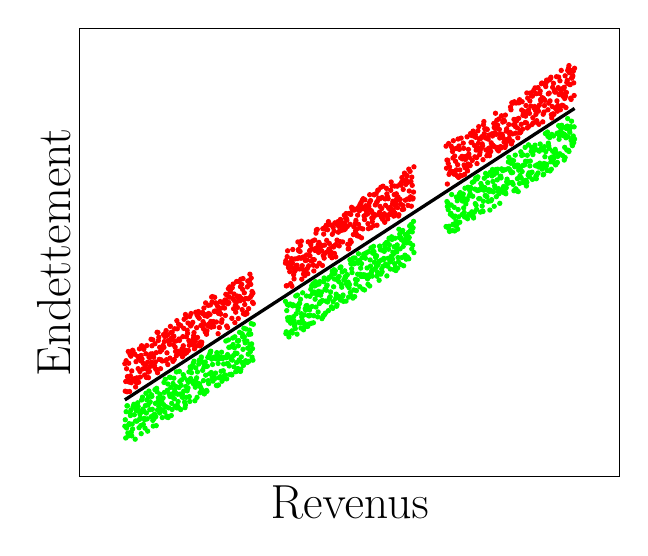
\begin{tikzpicture}


\begin{axis}[xtick=\empty, ytick=\empty, xlabel={\LARGE Revenus}, ylabel={\LARGE Endettement}]
\myGlobalTransformation{0}{0};

% pauvres
\addplot [green, only marks, mark=*, samples=300, mark size=0.75,domain=-3:1]{rand+x};
\addplot [red, only marks, mark=*, samples=300, mark size=0.75,domain=-3:1]{rand+x+2.5};

%moyens
\addplot [green, only marks, mark=*, samples=300, mark size=0.75,domain=2:6]{rand+x};
\addplot [red, only marks, mark=*, samples=300, mark size=0.75,domain=2:6]{rand+x+2.5};

%riches
\addplot [green, only marks, mark=*, samples=300, mark size=0.75,domain=7:11]{rand+x};
\addplot [red, only marks, mark=*, samples=300, mark size=0.75,domain=7:11]{rand+x+2.5};

%frontière
\addplot [black, very thick, domain=-3:11] {x+1.25};
\end{axis}


\end{tikzpicture}
\caption{\label{fig:xdiff} Multi-modal wages and indebtedness data generating mechanism with $y = \{0,1\}$ classes displayed in \textcolor{red}{red} and \textcolor{green}{green} respectively.}
\end{figure}

The second failing situation is the counterpart of the first tailored data generating mechanism. This time, suppose the covariates wages and indebtedness are uniformly sampled. Suppose there is a third categorical feature ``wages source'' which is drawn uniformly from three levels: renters, salaried workers and self-employed. One could argue that renters' risk level do not depend on their indebtedness, which is typically low (and a higher one is a major red flag), salaried workers' risk level is positively correlated with their indebtedness ratio as was the case for the first introductory example (see Figure~\ref{fig:xdiff}) and self-employed people's risk level is negatively correlated with this indebtedness ratio (say, the higher their personal engagement, the higher the chances of success of their business). This example data generating mechanism is illustrated on Figure~\ref{fig:ydiff}. In this situation, and contrary to the first example, an unsupervised generative clustering algorithm like \gls{pca} would not partition the data and the \textit{Credit Scoring} practitioner would construct only one scorecard. This scorecard would have high model bias since it is too simple to accommodate for the variety of the data generating mechanism and consequently perform poorly. This particular data generating mechanism is also revisited in the Experiments of Section~\ref{subsec:num_sim}.


\begin{figure}
\centering
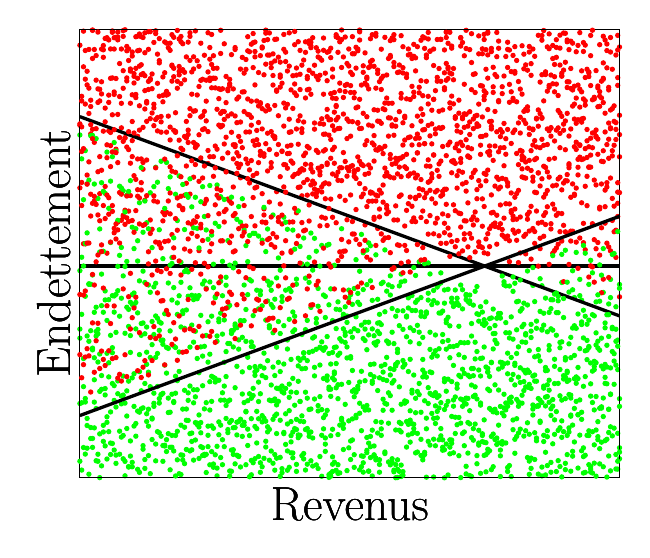
\begin{tikzpicture}


\begin{axis}[xtick=\empty, ytick=\empty, xlabel={\LARGE Revenus}, ylabel={\LARGE Endettement},domain=-3:1, enlargelimits=false,ymin=-3,ymax=6]
\myGlobalTransformationbis{0}{0};

% techniciens
\addplot [green, only marks, mark=*, samples=300, mark size=0.75,domain=-3:1]{rand};
\addplot [green, only marks, mark=*, samples=300, mark size=0.75,domain=-3:1]{rand-2};
\addplot [green, only marks, mark=*, samples=300, mark size=0.75,domain=-3:1]{rand-4};
\addplot [red, only marks, mark=*, samples=300, mark size=0.75,domain=-3:1]{rand+2.5};
\addplot [red, only marks, mark=*, samples=300, mark size=0.75,domain=-3:1]{rand+4.5};
\addplot [red, only marks, mark=*, samples=300, mark size=0.75,domain=-3:1]{rand+6.5};

%frontière
\addplot [black, very thick, domain=-3:1] {1.25};
\end{axis}





\begin{axis}[xtick=\empty, ytick=\empty, xlabel={\LARGE Revenus}, ylabel={\LARGE Endettement},domain=-3:1, enlargelimits=false,ymin=-3,ymax=6]
\myGlobalTransformationbis{0}{3};

% cadres
\addplot [green, only marks, mark=*, samples=300, mark size=0.75,domain=-3:1]{rand-x};
\addplot [green, only marks, mark=*, samples=300, mark size=0.75,domain=-3:1]{rand-x-2};
\addplot [green, only marks, mark=*, samples=300, mark size=0.75,domain=-3:1]{rand-x-4};
\addplot [red, only marks, mark=*, samples=300, mark size=0.75,domain=-3:1]{rand-x+2.5};
\addplot [red, only marks, mark=*, samples=300, mark size=0.75,domain=-3:1]{rand-x+4.5};
\addplot [red, only marks, mark=*, samples=300, mark size=0.75,domain=-3:1]{rand-x+6.5};

%frontière
\addplot [black, very thick, domain=-3:1] {-x+1.25};
\end{axis}



\begin{axis}[xtick=\empty, ytick=\empty, xlabel={\LARGE Revenus}, ylabel={\LARGE Endettement},domain=-3:1, enlargelimits=false,ymin=-3,ymax=6]
\myGlobalTransformationbis{0}{6};

% libérales
\addplot [green, only marks, mark=*, samples=300, mark size=0.75,domain=-3:1]{rand+x};
\addplot [green, only marks, mark=*, samples=300, mark size=0.75,domain=-3:1]{rand+x-2};
\addplot [green, only marks, mark=*, samples=300, mark size=0.75,domain=-3:1]{rand+x-4};
\addplot [red, only marks, mark=*, samples=300, mark size=0.75,domain=-3:1]{rand+x+2.5};
\addplot [red, only marks, mark=*, samples=300, mark size=0.75,domain=-3:1]{rand+x+4.5};
\addplot [red, only marks, mark=*, samples=300, mark size=0.75,domain=-3:1]{rand+x+6.5};
\addplot [red, only marks, mark=*, samples=300, mark size=0.75,domain=-3:1]{rand+x+8.5};

%frontière
\addplot [black, very thick, domain=-3:1] {x+1.25};
\end{axis}



\end{tikzpicture}
\caption{\label{fig:ydiff} Uni-modal wages and indebtedness data generating mechanism with $y = \{0,1\}$ classes displayed in \textcolor{red}{red} and \textcolor{green}{green} respectively which depends on a third feature.}
\end{figure}








\section{Literature review} \label{sec:literature}

This section aims at providing an eluded literature review of some well-known supervised clustering approaches that could be transposed to the \textit{Credit Scoring} industry.

\subsection{Supervised generative clustering methods} \label{subsec:sup_gen}

In the preceding section, examples of classical unsupervised clustering methods were given: \gls{pca} (continuous data), \gls{mca} (categorical data) and ultimately \gls{famd} (mixed data). In this section, focus is given to supervised generative methods. Indeed, a fully generative model $p(\gls{bx},y)$, if sufficiently flexible, could have easily spotted the bottlenecks of the failures of the \gls{pca} approach illustrated on Figures~\ref{fig:xdiff} and~\ref{fig:ydiff}.

\paragraph{\glsfirst{pls}}

The \gls{pls}~\cite{wold1984collinearity} algorithm seeks to combine the strengths, in its original proposal, of \gls{pca} in explaining the variance of the features $\gls{bx}$ and regression in predicting $y$ with the resulting principal components. In a classification setting, it is termed PLS-DA where DA stands for discriminant analysis.

The main idea is to construct a first component from the sum of the univariate regressions of $\gls{bbx}_j$ on $\gls{bby}$, then a second component from the sum of the univariate regressions of $\gls{bbx}_j$ subtracted by the first component on $\gls{bby}$, and so on. In a sense, a trade-off between reconstruction quality of $\gls{bbx}$ and $\gls{bby}$ with as few components as possible is achieved.

The \gls{pls} algorithm is given in Section~\ref{app1:sec_pls} of the Appendix, Algorithm~\ref{alg:pls}. It was used in~\cite{schwartz2009human} in a classification setting which results in Figure~\ref{fig:pca_vs_pls} reproduced with permission\footnote{\copyright 2009 IEEE}. It is striking how classes are better separated when using \gls{pls}. However, this does not guarantee that the resulting inferred segments' \gls{lr} will yield better predictive performance, considering that a \textit{Credit Scoring} practitioner would effectively spot two groups in Figure~\ref{fig:pca_vs_pls} (right) and separate them on the first \gls{pls} axis being above or below a threshold of approximately $0.01$. When applied to the Automobile dataset, it does not show such spectacular results (see Figure~\ref{fig:simu_pls}).

\begin{figure}
\includegraphics[width = \textwidth]{figures/chapitre6/pca_vs_pls.png}
\caption{Cloud points resulting from the application of \gls{pca} (left) and \gls{pls} (right) on a binary-labelled multivariate continuous dataset.}
\label{fig:pca_vs_pls}
\end{figure}

\begin{figure}
\centering \resizebox{.8\textwidth}{!}{% Created by tikzDevice version 0.12 on 2019-03-21 22:56:34
% !TEX encoding = UTF-8 Unicode
\begin{tikzpicture}[x=1pt,y=1pt]
\definecolor{fillColor}{RGB}{255,255,255}
\path[use as bounding box,fill=fillColor,fill opacity=0.00] (0,0) rectangle (867.24,433.62);
\begin{scope}
\path[clip] ( 49.20, 61.20) rectangle (842.04,384.42);
\definecolor{drawColor}{RGB}{255,0,0}

\path[draw=drawColor,line width= 0.4pt,line join=round,line cap=round] (355.07,343.32) circle (  2.25);
\definecolor{drawColor}{RGB}{0,0,0}

\path[draw=drawColor,line width= 0.4pt,line join=round,line cap=round] (115.53,323.32) circle (  2.25);
\definecolor{drawColor}{RGB}{255,0,0}

\path[draw=drawColor,line width= 0.4pt,line join=round,line cap=round] (180.86,330.01) circle (  2.25);

\path[draw=drawColor,line width= 0.4pt,line join=round,line cap=round] (160.38,335.55) circle (  2.25);

\path[draw=drawColor,line width= 0.4pt,line join=round,line cap=round] (124.98,330.72) circle (  2.25);

\path[draw=drawColor,line width= 0.4pt,line join=round,line cap=round] (271.66,243.29) circle (  2.25);

\path[draw=drawColor,line width= 0.4pt,line join=round,line cap=round] (252.49,297.36) circle (  2.25);

\path[draw=drawColor,line width= 0.4pt,line join=round,line cap=round] (165.77,314.59) circle (  2.25);

\path[draw=drawColor,line width= 0.4pt,line join=round,line cap=round] (214.39,318.40) circle (  2.25);

\path[draw=drawColor,line width= 0.4pt,line join=round,line cap=round] (144.64,342.78) circle (  2.25);

\path[draw=drawColor,line width= 0.4pt,line join=round,line cap=round] (258.74,336.13) circle (  2.25);

\path[draw=drawColor,line width= 0.4pt,line join=round,line cap=round] (184.61,281.51) circle (  2.25);

\path[draw=drawColor,line width= 0.4pt,line join=round,line cap=round] (120.99,294.62) circle (  2.25);

\path[draw=drawColor,line width= 0.4pt,line join=round,line cap=round] (207.15,331.02) circle (  2.25);

\path[draw=drawColor,line width= 0.4pt,line join=round,line cap=round] (175.57,240.13) circle (  2.25);

\path[draw=drawColor,line width= 0.4pt,line join=round,line cap=round] (114.83,318.98) circle (  2.25);

\path[draw=drawColor,line width= 0.4pt,line join=round,line cap=round] (167.84,328.62) circle (  2.25);

\path[draw=drawColor,line width= 0.4pt,line join=round,line cap=round] (133.36,308.54) circle (  2.25);

\path[draw=drawColor,line width= 0.4pt,line join=round,line cap=round] (376.96,293.37) circle (  2.25);

\path[draw=drawColor,line width= 0.4pt,line join=round,line cap=round] (141.05,322.44) circle (  2.25);

\path[draw=drawColor,line width= 0.4pt,line join=round,line cap=round] (128.58,279.71) circle (  2.25);

\path[draw=drawColor,line width= 0.4pt,line join=round,line cap=round] (212.89,332.37) circle (  2.25);

\path[draw=drawColor,line width= 0.4pt,line join=round,line cap=round] (215.96,318.62) circle (  2.25);

\path[draw=drawColor,line width= 0.4pt,line join=round,line cap=round] (125.50,283.35) circle (  2.25);

\path[draw=drawColor,line width= 0.4pt,line join=round,line cap=round] (166.24,332.20) circle (  2.25);

\path[draw=drawColor,line width= 0.4pt,line join=round,line cap=round] (173.92,330.35) circle (  2.25);

\path[draw=drawColor,line width= 0.4pt,line join=round,line cap=round] (140.45,252.93) circle (  2.25);

\path[draw=drawColor,line width= 0.4pt,line join=round,line cap=round] (119.21,316.26) circle (  2.25);

\path[draw=drawColor,line width= 0.4pt,line join=round,line cap=round] (116.55,324.78) circle (  2.25);

\path[draw=drawColor,line width= 0.4pt,line join=round,line cap=round] (188.77,148.51) circle (  2.25);

\path[draw=drawColor,line width= 0.4pt,line join=round,line cap=round] (131.34,252.04) circle (  2.25);

\path[draw=drawColor,line width= 0.4pt,line join=round,line cap=round] (123.68,331.68) circle (  2.25);

\path[draw=drawColor,line width= 0.4pt,line join=round,line cap=round] (218.65,341.10) circle (  2.25);

\path[draw=drawColor,line width= 0.4pt,line join=round,line cap=round] (128.61,318.71) circle (  2.25);

\path[draw=drawColor,line width= 0.4pt,line join=round,line cap=round] (131.80,261.37) circle (  2.25);

\path[draw=drawColor,line width= 0.4pt,line join=round,line cap=round] (125.23,287.79) circle (  2.25);

\path[draw=drawColor,line width= 0.4pt,line join=round,line cap=round] (149.56,315.02) circle (  2.25);

\path[draw=drawColor,line width= 0.4pt,line join=round,line cap=round] (169.34,253.59) circle (  2.25);

\path[draw=drawColor,line width= 0.4pt,line join=round,line cap=round] (120.22,304.22) circle (  2.25);

\path[draw=drawColor,line width= 0.4pt,line join=round,line cap=round] (120.31,287.40) circle (  2.25);

\path[draw=drawColor,line width= 0.4pt,line join=round,line cap=round] (120.35,319.61) circle (  2.25);

\path[draw=drawColor,line width= 0.4pt,line join=round,line cap=round] (254.17,346.85) circle (  2.25);

\path[draw=drawColor,line width= 0.4pt,line join=round,line cap=round] (190.06,332.23) circle (  2.25);

\path[draw=drawColor,line width= 0.4pt,line join=round,line cap=round] ( 84.97,239.61) circle (  2.25);

\path[draw=drawColor,line width= 0.4pt,line join=round,line cap=round] (119.88,337.15) circle (  2.25);

\path[draw=drawColor,line width= 0.4pt,line join=round,line cap=round] (142.77,332.45) circle (  2.25);

\path[draw=drawColor,line width= 0.4pt,line join=round,line cap=round] (171.92,338.00) circle (  2.25);

\path[draw=drawColor,line width= 0.4pt,line join=round,line cap=round] (199.64,248.52) circle (  2.25);

\path[draw=drawColor,line width= 0.4pt,line join=round,line cap=round] (135.94,302.71) circle (  2.25);
\definecolor{drawColor}{RGB}{0,0,0}

\path[draw=drawColor,line width= 0.4pt,line join=round,line cap=round] (128.20,320.04) circle (  2.25);

\path[draw=drawColor,line width= 0.4pt,line join=round,line cap=round] (137.70,303.41) circle (  2.25);
\definecolor{drawColor}{RGB}{255,0,0}

\path[draw=drawColor,line width= 0.4pt,line join=round,line cap=round] (176.48,329.92) circle (  2.25);

\path[draw=drawColor,line width= 0.4pt,line join=round,line cap=round] (220.71,314.62) circle (  2.25);

\path[draw=drawColor,line width= 0.4pt,line join=round,line cap=round] (285.33,330.55) circle (  2.25);

\path[draw=drawColor,line width= 0.4pt,line join=round,line cap=round] (113.43,282.02) circle (  2.25);

\path[draw=drawColor,line width= 0.4pt,line join=round,line cap=round] (256.54,347.17) circle (  2.25);

\path[draw=drawColor,line width= 0.4pt,line join=round,line cap=round] (224.16,282.08) circle (  2.25);

\path[draw=drawColor,line width= 0.4pt,line join=round,line cap=round] (181.60,222.68) circle (  2.25);

\path[draw=drawColor,line width= 0.4pt,line join=round,line cap=round] (177.19,326.25) circle (  2.25);

\path[draw=drawColor,line width= 0.4pt,line join=round,line cap=round] (123.62,309.58) circle (  2.25);

\path[draw=drawColor,line width= 0.4pt,line join=round,line cap=round] (174.47,254.40) circle (  2.25);

\path[draw=drawColor,line width= 0.4pt,line join=round,line cap=round] (218.52,334.40) circle (  2.25);

\path[draw=drawColor,line width= 0.4pt,line join=round,line cap=round] (123.60,326.52) circle (  2.25);

\path[draw=drawColor,line width= 0.4pt,line join=round,line cap=round] (133.08,293.78) circle (  2.25);

\path[draw=drawColor,line width= 0.4pt,line join=round,line cap=round] (162.43,174.48) circle (  2.25);

\path[draw=drawColor,line width= 0.4pt,line join=round,line cap=round] (112.17,322.10) circle (  2.25);

\path[draw=drawColor,line width= 0.4pt,line join=round,line cap=round] (172.99,324.59) circle (  2.25);

\path[draw=drawColor,line width= 0.4pt,line join=round,line cap=round] (277.55,279.07) circle (  2.25);

\path[draw=drawColor,line width= 0.4pt,line join=round,line cap=round] (218.71,328.70) circle (  2.25);

\path[draw=drawColor,line width= 0.4pt,line join=round,line cap=round] (207.73,341.62) circle (  2.25);

\path[draw=drawColor,line width= 0.4pt,line join=round,line cap=round] (124.56,313.06) circle (  2.25);

\path[draw=drawColor,line width= 0.4pt,line join=round,line cap=round] (137.49,277.27) circle (  2.25);

\path[draw=drawColor,line width= 0.4pt,line join=round,line cap=round] (229.67,324.58) circle (  2.25);

\path[draw=drawColor,line width= 0.4pt,line join=round,line cap=round] (127.29,293.15) circle (  2.25);

\path[draw=drawColor,line width= 0.4pt,line join=round,line cap=round] (260.98,327.96) circle (  2.25);

\path[draw=drawColor,line width= 0.4pt,line join=round,line cap=round] (197.20,314.00) circle (  2.25);

\path[draw=drawColor,line width= 0.4pt,line join=round,line cap=round] (167.32,300.17) circle (  2.25);

\path[draw=drawColor,line width= 0.4pt,line join=round,line cap=round] (154.82,292.56) circle (  2.25);

\path[draw=drawColor,line width= 0.4pt,line join=round,line cap=round] (178.82,325.65) circle (  2.25);

\path[draw=drawColor,line width= 0.4pt,line join=round,line cap=round] (126.15,296.84) circle (  2.25);

\path[draw=drawColor,line width= 0.4pt,line join=round,line cap=round] (187.68,291.67) circle (  2.25);

\path[draw=drawColor,line width= 0.4pt,line join=round,line cap=round] (115.02,316.51) circle (  2.25);

\path[draw=drawColor,line width= 0.4pt,line join=round,line cap=round] (113.67,333.65) circle (  2.25);

\path[draw=drawColor,line width= 0.4pt,line join=round,line cap=round] (213.39,334.22) circle (  2.25);

\path[draw=drawColor,line width= 0.4pt,line join=round,line cap=round] (124.29,304.32) circle (  2.25);

\path[draw=drawColor,line width= 0.4pt,line join=round,line cap=round] (170.24,320.62) circle (  2.25);

\path[draw=drawColor,line width= 0.4pt,line join=round,line cap=round] (134.24,269.68) circle (  2.25);

\path[draw=drawColor,line width= 0.4pt,line join=round,line cap=round] (155.31,333.03) circle (  2.25);

\path[draw=drawColor,line width= 0.4pt,line join=round,line cap=round] (107.35,285.58) circle (  2.25);

\path[draw=drawColor,line width= 0.4pt,line join=round,line cap=round] (135.68,288.07) circle (  2.25);

\path[draw=drawColor,line width= 0.4pt,line join=round,line cap=round] (116.91,295.60) circle (  2.25);

\path[draw=drawColor,line width= 0.4pt,line join=round,line cap=round] (188.04, 73.17) circle (  2.25);

\path[draw=drawColor,line width= 0.4pt,line join=round,line cap=round] (129.63,310.98) circle (  2.25);

\path[draw=drawColor,line width= 0.4pt,line join=round,line cap=round] (138.83,322.24) circle (  2.25);

\path[draw=drawColor,line width= 0.4pt,line join=round,line cap=round] ( 88.79,256.78) circle (  2.25);

\path[draw=drawColor,line width= 0.4pt,line join=round,line cap=round] (235.28,261.76) circle (  2.25);

\path[draw=drawColor,line width= 0.4pt,line join=round,line cap=round] (107.85,317.53) circle (  2.25);

\path[draw=drawColor,line width= 0.4pt,line join=round,line cap=round] (142.27,275.65) circle (  2.25);

\path[draw=drawColor,line width= 0.4pt,line join=round,line cap=round] (309.58,292.21) circle (  2.25);

\path[draw=drawColor,line width= 0.4pt,line join=round,line cap=round] (195.29,328.66) circle (  2.25);

\path[draw=drawColor,line width= 0.4pt,line join=round,line cap=round] (148.87,265.15) circle (  2.25);
\definecolor{drawColor}{RGB}{0,0,0}

\path[draw=drawColor,line width= 0.4pt,line join=round,line cap=round] (141.77,312.16) circle (  2.25);

\path[draw=drawColor,line width= 0.4pt,line join=round,line cap=round] (118.25,300.82) circle (  2.25);
\definecolor{drawColor}{RGB}{255,0,0}

\path[draw=drawColor,line width= 0.4pt,line join=round,line cap=round] (142.94,328.42) circle (  2.25);

\path[draw=drawColor,line width= 0.4pt,line join=round,line cap=round] (134.72,273.98) circle (  2.25);

\path[draw=drawColor,line width= 0.4pt,line join=round,line cap=round] (187.98,292.39) circle (  2.25);

\path[draw=drawColor,line width= 0.4pt,line join=round,line cap=round] (137.86,245.53) circle (  2.25);
\definecolor{drawColor}{RGB}{0,0,0}

\path[draw=drawColor,line width= 0.4pt,line join=round,line cap=round] (159.90,263.06) circle (  2.25);
\definecolor{drawColor}{RGB}{255,0,0}

\path[draw=drawColor,line width= 0.4pt,line join=round,line cap=round] (125.36,318.78) circle (  2.25);
\definecolor{drawColor}{RGB}{0,0,0}

\path[draw=drawColor,line width= 0.4pt,line join=round,line cap=round] (123.80,266.36) circle (  2.25);
\definecolor{drawColor}{RGB}{255,0,0}

\path[draw=drawColor,line width= 0.4pt,line join=round,line cap=round] (157.95,282.87) circle (  2.25);

\path[draw=drawColor,line width= 0.4pt,line join=round,line cap=round] (114.54,311.29) circle (  2.25);

\path[draw=drawColor,line width= 0.4pt,line join=round,line cap=round] (134.92,340.14) circle (  2.25);

\path[draw=drawColor,line width= 0.4pt,line join=round,line cap=round] (218.17,327.71) circle (  2.25);

\path[draw=drawColor,line width= 0.4pt,line join=round,line cap=round] (129.32,282.77) circle (  2.25);

\path[draw=drawColor,line width= 0.4pt,line join=round,line cap=round] (123.64,290.71) circle (  2.25);

\path[draw=drawColor,line width= 0.4pt,line join=round,line cap=round] (117.72,332.47) circle (  2.25);

\path[draw=drawColor,line width= 0.4pt,line join=round,line cap=round] (127.88,311.83) circle (  2.25);

\path[draw=drawColor,line width= 0.4pt,line join=round,line cap=round] (161.73,310.03) circle (  2.25);

\path[draw=drawColor,line width= 0.4pt,line join=round,line cap=round] (160.96,328.46) circle (  2.25);

\path[draw=drawColor,line width= 0.4pt,line join=round,line cap=round] (274.36,349.98) circle (  2.25);

\path[draw=drawColor,line width= 0.4pt,line join=round,line cap=round] (121.66,286.36) circle (  2.25);

\path[draw=drawColor,line width= 0.4pt,line join=round,line cap=round] (168.46,327.81) circle (  2.25);

\path[draw=drawColor,line width= 0.4pt,line join=round,line cap=round] (224.75,330.81) circle (  2.25);

\path[draw=drawColor,line width= 0.4pt,line join=round,line cap=round] (174.69,264.42) circle (  2.25);

\path[draw=drawColor,line width= 0.4pt,line join=round,line cap=round] (129.29,235.07) circle (  2.25);

\path[draw=drawColor,line width= 0.4pt,line join=round,line cap=round] (124.51,257.30) circle (  2.25);

\path[draw=drawColor,line width= 0.4pt,line join=round,line cap=round] (122.92,296.90) circle (  2.25);

\path[draw=drawColor,line width= 0.4pt,line join=round,line cap=round] (111.98,318.78) circle (  2.25);

\path[draw=drawColor,line width= 0.4pt,line join=round,line cap=round] (159.03,281.90) circle (  2.25);
\definecolor{drawColor}{RGB}{0,0,0}

\path[draw=drawColor,line width= 0.4pt,line join=round,line cap=round] (153.49,259.06) circle (  2.25);
\definecolor{drawColor}{RGB}{255,0,0}

\path[draw=drawColor,line width= 0.4pt,line join=round,line cap=round] (136.55,338.04) circle (  2.25);

\path[draw=drawColor,line width= 0.4pt,line join=round,line cap=round] (218.16,268.87) circle (  2.25);

\path[draw=drawColor,line width= 0.4pt,line join=round,line cap=round] (138.00,305.03) circle (  2.25);

\path[draw=drawColor,line width= 0.4pt,line join=round,line cap=round] (115.22,336.99) circle (  2.25);

\path[draw=drawColor,line width= 0.4pt,line join=round,line cap=round] (151.46,317.73) circle (  2.25);

\path[draw=drawColor,line width= 0.4pt,line join=round,line cap=round] (119.13,326.55) circle (  2.25);

\path[draw=drawColor,line width= 0.4pt,line join=round,line cap=round] (157.15,337.70) circle (  2.25);

\path[draw=drawColor,line width= 0.4pt,line join=round,line cap=round] (131.04,309.71) circle (  2.25);

\path[draw=drawColor,line width= 0.4pt,line join=round,line cap=round] (124.76,283.89) circle (  2.25);

\path[draw=drawColor,line width= 0.4pt,line join=round,line cap=round] (146.75,240.08) circle (  2.25);

\path[draw=drawColor,line width= 0.4pt,line join=round,line cap=round] (253.61,339.76) circle (  2.25);

\path[draw=drawColor,line width= 0.4pt,line join=round,line cap=round] (167.74,249.39) circle (  2.25);

\path[draw=drawColor,line width= 0.4pt,line join=round,line cap=round] (133.47,321.20) circle (  2.25);

\path[draw=drawColor,line width= 0.4pt,line join=round,line cap=round] (110.93,295.59) circle (  2.25);

\path[draw=drawColor,line width= 0.4pt,line join=round,line cap=round] (142.63,277.85) circle (  2.25);

\path[draw=drawColor,line width= 0.4pt,line join=round,line cap=round] (425.42,343.96) circle (  2.25);

\path[draw=drawColor,line width= 0.4pt,line join=round,line cap=round] (175.87,320.51) circle (  2.25);

\path[draw=drawColor,line width= 0.4pt,line join=round,line cap=round] (273.74,331.71) circle (  2.25);

\path[draw=drawColor,line width= 0.4pt,line join=round,line cap=round] (172.36,278.06) circle (  2.25);

\path[draw=drawColor,line width= 0.4pt,line join=round,line cap=round] (114.63,299.25) circle (  2.25);

\path[draw=drawColor,line width= 0.4pt,line join=round,line cap=round] (214.04,272.27) circle (  2.25);

\path[draw=drawColor,line width= 0.4pt,line join=round,line cap=round] (211.81,301.20) circle (  2.25);

\path[draw=drawColor,line width= 0.4pt,line join=round,line cap=round] (163.85,311.47) circle (  2.25);

\path[draw=drawColor,line width= 0.4pt,line join=round,line cap=round] (235.60,331.13) circle (  2.25);

\path[draw=drawColor,line width= 0.4pt,line join=round,line cap=round] (243.31,329.92) circle (  2.25);

\path[draw=drawColor,line width= 0.4pt,line join=round,line cap=round] (226.63,276.95) circle (  2.25);

\path[draw=drawColor,line width= 0.4pt,line join=round,line cap=round] (241.63,347.68) circle (  2.25);

\path[draw=drawColor,line width= 0.4pt,line join=round,line cap=round] (213.44,335.13) circle (  2.25);

\path[draw=drawColor,line width= 0.4pt,line join=round,line cap=round] (122.83,326.70) circle (  2.25);

\path[draw=drawColor,line width= 0.4pt,line join=round,line cap=round] (152.71,274.68) circle (  2.25);

\path[draw=drawColor,line width= 0.4pt,line join=round,line cap=round] (140.49,339.32) circle (  2.25);

\path[draw=drawColor,line width= 0.4pt,line join=round,line cap=round] (180.25,330.09) circle (  2.25);

\path[draw=drawColor,line width= 0.4pt,line join=round,line cap=round] (130.35,275.29) circle (  2.25);

\path[draw=drawColor,line width= 0.4pt,line join=round,line cap=round] (242.26,306.93) circle (  2.25);

\path[draw=drawColor,line width= 0.4pt,line join=round,line cap=round] (115.51,340.45) circle (  2.25);

\path[draw=drawColor,line width= 0.4pt,line join=round,line cap=round] (197.15,198.50) circle (  2.25);

\path[draw=drawColor,line width= 0.4pt,line join=round,line cap=round] (155.25,284.22) circle (  2.25);
\definecolor{drawColor}{RGB}{0,0,0}

\path[draw=drawColor,line width= 0.4pt,line join=round,line cap=round] (147.53,330.75) circle (  2.25);
\definecolor{drawColor}{RGB}{255,0,0}

\path[draw=drawColor,line width= 0.4pt,line join=round,line cap=round] (241.02,327.15) circle (  2.25);

\path[draw=drawColor,line width= 0.4pt,line join=round,line cap=round] (125.82,316.75) circle (  2.25);

\path[draw=drawColor,line width= 0.4pt,line join=round,line cap=round] (812.68,338.50) circle (  2.25);

\path[draw=drawColor,line width= 0.4pt,line join=round,line cap=round] (130.64,326.13) circle (  2.25);

\path[draw=drawColor,line width= 0.4pt,line join=round,line cap=round] (139.37,281.61) circle (  2.25);

\path[draw=drawColor,line width= 0.4pt,line join=round,line cap=round] (317.33,338.68) circle (  2.25);

\path[draw=drawColor,line width= 0.4pt,line join=round,line cap=round] (106.49,280.05) circle (  2.25);

\path[draw=drawColor,line width= 0.4pt,line join=round,line cap=round] (123.72,285.40) circle (  2.25);

\path[draw=drawColor,line width= 0.4pt,line join=round,line cap=round] (190.08,318.28) circle (  2.25);

\path[draw=drawColor,line width= 0.4pt,line join=round,line cap=round] (190.42,334.25) circle (  2.25);

\path[draw=drawColor,line width= 0.4pt,line join=round,line cap=round] (153.94,327.37) circle (  2.25);

\path[draw=drawColor,line width= 0.4pt,line join=round,line cap=round] (254.75,326.63) circle (  2.25);

\path[draw=drawColor,line width= 0.4pt,line join=round,line cap=round] (137.43,308.62) circle (  2.25);

\path[draw=drawColor,line width= 0.4pt,line join=round,line cap=round] (117.42,334.72) circle (  2.25);

\path[draw=drawColor,line width= 0.4pt,line join=round,line cap=round] (130.10,300.64) circle (  2.25);

\path[draw=drawColor,line width= 0.4pt,line join=round,line cap=round] (126.95,267.78) circle (  2.25);

\path[draw=drawColor,line width= 0.4pt,line join=round,line cap=round] (147.54,339.55) circle (  2.25);

\path[draw=drawColor,line width= 0.4pt,line join=round,line cap=round] (214.22,162.69) circle (  2.25);

\path[draw=drawColor,line width= 0.4pt,line join=round,line cap=round] (140.58,283.99) circle (  2.25);

\path[draw=drawColor,line width= 0.4pt,line join=round,line cap=round] (216.99,262.10) circle (  2.25);

\path[draw=drawColor,line width= 0.4pt,line join=round,line cap=round] (154.96,231.19) circle (  2.25);

\path[draw=drawColor,line width= 0.4pt,line join=round,line cap=round] (161.02,278.99) circle (  2.25);

\path[draw=drawColor,line width= 0.4pt,line join=round,line cap=round] (116.63,327.71) circle (  2.25);

\path[draw=drawColor,line width= 0.4pt,line join=round,line cap=round] ( 83.18,221.57) circle (  2.25);

\path[draw=drawColor,line width= 0.4pt,line join=round,line cap=round] (149.60,318.05) circle (  2.25);

\path[draw=drawColor,line width= 0.4pt,line join=round,line cap=round] (149.81,263.46) circle (  2.25);

\path[draw=drawColor,line width= 0.4pt,line join=round,line cap=round] (220.10,182.78) circle (  2.25);

\path[draw=drawColor,line width= 0.4pt,line join=round,line cap=round] (124.23,313.10) circle (  2.25);

\path[draw=drawColor,line width= 0.4pt,line join=round,line cap=round] (168.71,326.39) circle (  2.25);

\path[draw=drawColor,line width= 0.4pt,line join=round,line cap=round] (114.93,308.01) circle (  2.25);

\path[draw=drawColor,line width= 0.4pt,line join=round,line cap=round] (118.10,318.29) circle (  2.25);

\path[draw=drawColor,line width= 0.4pt,line join=round,line cap=round] (139.50,265.03) circle (  2.25);

\path[draw=drawColor,line width= 0.4pt,line join=round,line cap=round] (167.67,319.30) circle (  2.25);

\path[draw=drawColor,line width= 0.4pt,line join=round,line cap=round] (140.45,343.00) circle (  2.25);

\path[draw=drawColor,line width= 0.4pt,line join=round,line cap=round] (156.71,304.88) circle (  2.25);

\path[draw=drawColor,line width= 0.4pt,line join=round,line cap=round] (124.20,294.02) circle (  2.25);

\path[draw=drawColor,line width= 0.4pt,line join=round,line cap=round] (160.50,284.42) circle (  2.25);

\path[draw=drawColor,line width= 0.4pt,line join=round,line cap=round] (132.07,316.45) circle (  2.25);

\path[draw=drawColor,line width= 0.4pt,line join=round,line cap=round] (159.72,178.12) circle (  2.25);

\path[draw=drawColor,line width= 0.4pt,line join=round,line cap=round] (117.71,305.69) circle (  2.25);

\path[draw=drawColor,line width= 0.4pt,line join=round,line cap=round] (268.62,304.74) circle (  2.25);

\path[draw=drawColor,line width= 0.4pt,line join=round,line cap=round] (147.46,280.81) circle (  2.25);

\path[draw=drawColor,line width= 0.4pt,line join=round,line cap=round] (134.07,280.28) circle (  2.25);

\path[draw=drawColor,line width= 0.4pt,line join=round,line cap=round] (216.84,302.06) circle (  2.25);

\path[draw=drawColor,line width= 0.4pt,line join=round,line cap=round] (133.90,334.48) circle (  2.25);

\path[draw=drawColor,line width= 0.4pt,line join=round,line cap=round] (211.91,333.55) circle (  2.25);

\path[draw=drawColor,line width= 0.4pt,line join=round,line cap=round] (117.53,340.34) circle (  2.25);

\path[draw=drawColor,line width= 0.4pt,line join=round,line cap=round] (187.37,303.04) circle (  2.25);

\path[draw=drawColor,line width= 0.4pt,line join=round,line cap=round] (111.64,298.77) circle (  2.25);

\path[draw=drawColor,line width= 0.4pt,line join=round,line cap=round] (123.74,293.76) circle (  2.25);

\path[draw=drawColor,line width= 0.4pt,line join=round,line cap=round] (163.05,274.06) circle (  2.25);

\path[draw=drawColor,line width= 0.4pt,line join=round,line cap=round] (125.97,293.13) circle (  2.25);

\path[draw=drawColor,line width= 0.4pt,line join=round,line cap=round] (119.65,329.15) circle (  2.25);

\path[draw=drawColor,line width= 0.4pt,line join=round,line cap=round] (131.46,292.02) circle (  2.25);

\path[draw=drawColor,line width= 0.4pt,line join=round,line cap=round] (165.99,285.88) circle (  2.25);

\path[draw=drawColor,line width= 0.4pt,line join=round,line cap=round] (145.57,303.56) circle (  2.25);

\path[draw=drawColor,line width= 0.4pt,line join=round,line cap=round] (131.33,288.22) circle (  2.25);

\path[draw=drawColor,line width= 0.4pt,line join=round,line cap=round] (213.63,341.58) circle (  2.25);

\path[draw=drawColor,line width= 0.4pt,line join=round,line cap=round] (184.35,222.23) circle (  2.25);

\path[draw=drawColor,line width= 0.4pt,line join=round,line cap=round] (131.53,280.55) circle (  2.25);

\path[draw=drawColor,line width= 0.4pt,line join=round,line cap=round] (130.35,308.77) circle (  2.25);

\path[draw=drawColor,line width= 0.4pt,line join=round,line cap=round] (119.36,284.79) circle (  2.25);

\path[draw=drawColor,line width= 0.4pt,line join=round,line cap=round] (180.42,344.29) circle (  2.25);

\path[draw=drawColor,line width= 0.4pt,line join=round,line cap=round] (148.65,186.83) circle (  2.25);

\path[draw=drawColor,line width= 0.4pt,line join=round,line cap=round] (185.95,335.19) circle (  2.25);

\path[draw=drawColor,line width= 0.4pt,line join=round,line cap=round] (130.59,343.99) circle (  2.25);

\path[draw=drawColor,line width= 0.4pt,line join=round,line cap=round] (170.12,345.61) circle (  2.25);

\path[draw=drawColor,line width= 0.4pt,line join=round,line cap=round] (114.92,303.03) circle (  2.25);

\path[draw=drawColor,line width= 0.4pt,line join=round,line cap=round] (311.84,212.04) circle (  2.25);

\path[draw=drawColor,line width= 0.4pt,line join=round,line cap=round] (166.46,285.76) circle (  2.25);

\path[draw=drawColor,line width= 0.4pt,line join=round,line cap=round] (207.89,340.31) circle (  2.25);

\path[draw=drawColor,line width= 0.4pt,line join=round,line cap=round] (151.46,295.33) circle (  2.25);

\path[draw=drawColor,line width= 0.4pt,line join=round,line cap=round] (113.06,336.18) circle (  2.25);

\path[draw=drawColor,line width= 0.4pt,line join=round,line cap=round] (130.96,285.91) circle (  2.25);

\path[draw=drawColor,line width= 0.4pt,line join=round,line cap=round] (118.71,291.52) circle (  2.25);

\path[draw=drawColor,line width= 0.4pt,line join=round,line cap=round] (117.75,284.01) circle (  2.25);

\path[draw=drawColor,line width= 0.4pt,line join=round,line cap=round] (120.73,291.71) circle (  2.25);

\path[draw=drawColor,line width= 0.4pt,line join=round,line cap=round] (124.93,284.30) circle (  2.25);

\path[draw=drawColor,line width= 0.4pt,line join=round,line cap=round] (124.43,275.36) circle (  2.25);

\path[draw=drawColor,line width= 0.4pt,line join=round,line cap=round] (154.91,298.62) circle (  2.25);

\path[draw=drawColor,line width= 0.4pt,line join=round,line cap=round] (122.98,286.37) circle (  2.25);

\path[draw=drawColor,line width= 0.4pt,line join=round,line cap=round] (187.95,339.30) circle (  2.25);

\path[draw=drawColor,line width= 0.4pt,line join=round,line cap=round] (128.19,247.21) circle (  2.25);

\path[draw=drawColor,line width= 0.4pt,line join=round,line cap=round] (126.97,290.37) circle (  2.25);

\path[draw=drawColor,line width= 0.4pt,line join=round,line cap=round] (109.69,315.16) circle (  2.25);

\path[draw=drawColor,line width= 0.4pt,line join=round,line cap=round] (147.41,305.87) circle (  2.25);

\path[draw=drawColor,line width= 0.4pt,line join=round,line cap=round] (161.76,310.70) circle (  2.25);

\path[draw=drawColor,line width= 0.4pt,line join=round,line cap=round] (132.39,319.19) circle (  2.25);

\path[draw=drawColor,line width= 0.4pt,line join=round,line cap=round] (112.84,325.34) circle (  2.25);

\path[draw=drawColor,line width= 0.4pt,line join=round,line cap=round] (151.99,271.60) circle (  2.25);

\path[draw=drawColor,line width= 0.4pt,line join=round,line cap=round] (121.73,284.06) circle (  2.25);

\path[draw=drawColor,line width= 0.4pt,line join=round,line cap=round] (306.76,280.10) circle (  2.25);

\path[draw=drawColor,line width= 0.4pt,line join=round,line cap=round] (185.27,165.90) circle (  2.25);

\path[draw=drawColor,line width= 0.4pt,line join=round,line cap=round] (128.73,324.85) circle (  2.25);

\path[draw=drawColor,line width= 0.4pt,line join=round,line cap=round] (144.43,329.33) circle (  2.25);

\path[draw=drawColor,line width= 0.4pt,line join=round,line cap=round] (118.57,303.58) circle (  2.25);

\path[draw=drawColor,line width= 0.4pt,line join=round,line cap=round] (155.44,344.34) circle (  2.25);

\path[draw=drawColor,line width= 0.4pt,line join=round,line cap=round] (160.21,281.49) circle (  2.25);

\path[draw=drawColor,line width= 0.4pt,line join=round,line cap=round] (110.68,322.70) circle (  2.25);

\path[draw=drawColor,line width= 0.4pt,line join=round,line cap=round] (115.73,323.88) circle (  2.25);

\path[draw=drawColor,line width= 0.4pt,line join=round,line cap=round] (171.85,338.96) circle (  2.25);

\path[draw=drawColor,line width= 0.4pt,line join=round,line cap=round] (188.38,325.57) circle (  2.25);

\path[draw=drawColor,line width= 0.4pt,line join=round,line cap=round] (126.83,290.39) circle (  2.25);

\path[draw=drawColor,line width= 0.4pt,line join=round,line cap=round] (113.41,340.47) circle (  2.25);

\path[draw=drawColor,line width= 0.4pt,line join=round,line cap=round] (121.65,306.74) circle (  2.25);

\path[draw=drawColor,line width= 0.4pt,line join=round,line cap=round] (128.95,293.65) circle (  2.25);

\path[draw=drawColor,line width= 0.4pt,line join=round,line cap=round] (163.52,239.31) circle (  2.25);

\path[draw=drawColor,line width= 0.4pt,line join=round,line cap=round] (130.80,286.28) circle (  2.25);

\path[draw=drawColor,line width= 0.4pt,line join=round,line cap=round] (153.69,325.86) circle (  2.25);

\path[draw=drawColor,line width= 0.4pt,line join=round,line cap=round] (464.40,235.40) circle (  2.25);
\definecolor{drawColor}{RGB}{0,0,0}

\path[draw=drawColor,line width= 0.4pt,line join=round,line cap=round] (155.90,316.19) circle (  2.25);
\definecolor{drawColor}{RGB}{255,0,0}

\path[draw=drawColor,line width= 0.4pt,line join=round,line cap=round] (121.84,302.80) circle (  2.25);

\path[draw=drawColor,line width= 0.4pt,line join=round,line cap=round] (124.34,331.59) circle (  2.25);

\path[draw=drawColor,line width= 0.4pt,line join=round,line cap=round] (300.52,348.83) circle (  2.25);

\path[draw=drawColor,line width= 0.4pt,line join=round,line cap=round] (140.66,342.54) circle (  2.25);

\path[draw=drawColor,line width= 0.4pt,line join=round,line cap=round] (177.42,327.68) circle (  2.25);

\path[draw=drawColor,line width= 0.4pt,line join=round,line cap=round] (161.42,337.87) circle (  2.25);

\path[draw=drawColor,line width= 0.4pt,line join=round,line cap=round] (261.64,308.99) circle (  2.25);

\path[draw=drawColor,line width= 0.4pt,line join=round,line cap=round] (146.97,326.39) circle (  2.25);

\path[draw=drawColor,line width= 0.4pt,line join=round,line cap=round] (121.49,341.59) circle (  2.25);

\path[draw=drawColor,line width= 0.4pt,line join=round,line cap=round] (127.79,278.98) circle (  2.25);

\path[draw=drawColor,line width= 0.4pt,line join=round,line cap=round] (118.89,329.83) circle (  2.25);

\path[draw=drawColor,line width= 0.4pt,line join=round,line cap=round] (131.89,311.82) circle (  2.25);

\path[draw=drawColor,line width= 0.4pt,line join=round,line cap=round] (341.56,334.86) circle (  2.25);

\path[draw=drawColor,line width= 0.4pt,line join=round,line cap=round] (198.99,320.64) circle (  2.25);

\path[draw=drawColor,line width= 0.4pt,line join=round,line cap=round] (126.20,270.96) circle (  2.25);

\path[draw=drawColor,line width= 0.4pt,line join=round,line cap=round] (126.56,286.39) circle (  2.25);

\path[draw=drawColor,line width= 0.4pt,line join=round,line cap=round] (131.04,290.51) circle (  2.25);

\path[draw=drawColor,line width= 0.4pt,line join=round,line cap=round] (133.69,332.43) circle (  2.25);

\path[draw=drawColor,line width= 0.4pt,line join=round,line cap=round] (174.84,327.42) circle (  2.25);

\path[draw=drawColor,line width= 0.4pt,line join=round,line cap=round] (295.87,335.21) circle (  2.25);

\path[draw=drawColor,line width= 0.4pt,line join=round,line cap=round] (239.55,327.40) circle (  2.25);

\path[draw=drawColor,line width= 0.4pt,line join=round,line cap=round] (147.03,288.47) circle (  2.25);

\path[draw=drawColor,line width= 0.4pt,line join=round,line cap=round] (116.20,323.58) circle (  2.25);

\path[draw=drawColor,line width= 0.4pt,line join=round,line cap=round] (179.37,266.82) circle (  2.25);
\definecolor{drawColor}{RGB}{0,0,0}

\path[draw=drawColor,line width= 0.4pt,line join=round,line cap=round] (143.77,201.71) circle (  2.25);
\definecolor{drawColor}{RGB}{255,0,0}

\path[draw=drawColor,line width= 0.4pt,line join=round,line cap=round] (137.56,291.85) circle (  2.25);

\path[draw=drawColor,line width= 0.4pt,line join=round,line cap=round] (171.26,293.74) circle (  2.25);

\path[draw=drawColor,line width= 0.4pt,line join=round,line cap=round] (113.94,340.68) circle (  2.25);

\path[draw=drawColor,line width= 0.4pt,line join=round,line cap=round] (141.11,278.47) circle (  2.25);

\path[draw=drawColor,line width= 0.4pt,line join=round,line cap=round] (123.39,292.43) circle (  2.25);

\path[draw=drawColor,line width= 0.4pt,line join=round,line cap=round] (158.04,266.52) circle (  2.25);

\path[draw=drawColor,line width= 0.4pt,line join=round,line cap=round] (185.19,324.45) circle (  2.25);

\path[draw=drawColor,line width= 0.4pt,line join=round,line cap=round] (170.89,243.99) circle (  2.25);
\definecolor{drawColor}{RGB}{0,0,0}

\path[draw=drawColor,line width= 0.4pt,line join=round,line cap=round] (121.75,292.27) circle (  2.25);
\definecolor{drawColor}{RGB}{255,0,0}

\path[draw=drawColor,line width= 0.4pt,line join=round,line cap=round] (128.67,315.23) circle (  2.25);

\path[draw=drawColor,line width= 0.4pt,line join=round,line cap=round] (140.69,271.67) circle (  2.25);

\path[draw=drawColor,line width= 0.4pt,line join=round,line cap=round] (223.80,316.33) circle (  2.25);

\path[draw=drawColor,line width= 0.4pt,line join=round,line cap=round] (137.57,249.69) circle (  2.25);

\path[draw=drawColor,line width= 0.4pt,line join=round,line cap=round] (114.19,344.13) circle (  2.25);

\path[draw=drawColor,line width= 0.4pt,line join=round,line cap=round] (118.96,317.58) circle (  2.25);

\path[draw=drawColor,line width= 0.4pt,line join=round,line cap=round] (152.51,252.08) circle (  2.25);

\path[draw=drawColor,line width= 0.4pt,line join=round,line cap=round] (119.03,305.85) circle (  2.25);

\path[draw=drawColor,line width= 0.4pt,line join=round,line cap=round] (132.21,313.16) circle (  2.25);

\path[draw=drawColor,line width= 0.4pt,line join=round,line cap=round] (178.67,295.32) circle (  2.25);

\path[draw=drawColor,line width= 0.4pt,line join=round,line cap=round] (177.60,302.51) circle (  2.25);

\path[draw=drawColor,line width= 0.4pt,line join=round,line cap=round] (137.21,332.88) circle (  2.25);

\path[draw=drawColor,line width= 0.4pt,line join=round,line cap=round] (142.75,262.61) circle (  2.25);

\path[draw=drawColor,line width= 0.4pt,line join=round,line cap=round] (147.46,245.47) circle (  2.25);

\path[draw=drawColor,line width= 0.4pt,line join=round,line cap=round] (116.53,312.29) circle (  2.25);

\path[draw=drawColor,line width= 0.4pt,line join=round,line cap=round] (220.82,330.88) circle (  2.25);

\path[draw=drawColor,line width= 0.4pt,line join=round,line cap=round] (132.43,259.02) circle (  2.25);

\path[draw=drawColor,line width= 0.4pt,line join=round,line cap=round] (176.49,335.43) circle (  2.25);

\path[draw=drawColor,line width= 0.4pt,line join=round,line cap=round] (113.88,309.94) circle (  2.25);

\path[draw=drawColor,line width= 0.4pt,line join=round,line cap=round] (208.50,327.81) circle (  2.25);

\path[draw=drawColor,line width= 0.4pt,line join=round,line cap=round] (227.62,299.81) circle (  2.25);

\path[draw=drawColor,line width= 0.4pt,line join=round,line cap=round] (175.01,268.79) circle (  2.25);

\path[draw=drawColor,line width= 0.4pt,line join=round,line cap=round] (175.70,309.62) circle (  2.25);

\path[draw=drawColor,line width= 0.4pt,line join=round,line cap=round] (117.26,312.85) circle (  2.25);

\path[draw=drawColor,line width= 0.4pt,line join=round,line cap=round] (111.32,320.12) circle (  2.25);
\definecolor{drawColor}{RGB}{0,0,0}

\path[draw=drawColor,line width= 0.4pt,line join=round,line cap=round] (115.37,283.32) circle (  2.25);
\definecolor{drawColor}{RGB}{255,0,0}

\path[draw=drawColor,line width= 0.4pt,line join=round,line cap=round] (118.67,307.19) circle (  2.25);

\path[draw=drawColor,line width= 0.4pt,line join=round,line cap=round] (233.48,329.76) circle (  2.25);

\path[draw=drawColor,line width= 0.4pt,line join=round,line cap=round] (138.77,332.78) circle (  2.25);

\path[draw=drawColor,line width= 0.4pt,line join=round,line cap=round] (173.12,330.37) circle (  2.25);

\path[draw=drawColor,line width= 0.4pt,line join=round,line cap=round] (167.38,226.91) circle (  2.25);

\path[draw=drawColor,line width= 0.4pt,line join=round,line cap=round] (106.54,295.55) circle (  2.25);

\path[draw=drawColor,line width= 0.4pt,line join=round,line cap=round] (195.43,330.73) circle (  2.25);

\path[draw=drawColor,line width= 0.4pt,line join=round,line cap=round] (121.91,302.48) circle (  2.25);

\path[draw=drawColor,line width= 0.4pt,line join=round,line cap=round] (117.02,311.88) circle (  2.25);

\path[draw=drawColor,line width= 0.4pt,line join=round,line cap=round] (151.09,335.62) circle (  2.25);

\path[draw=drawColor,line width= 0.4pt,line join=round,line cap=round] (121.11,321.35) circle (  2.25);

\path[draw=drawColor,line width= 0.4pt,line join=round,line cap=round] (124.11,293.44) circle (  2.25);
\definecolor{drawColor}{RGB}{0,0,0}

\path[draw=drawColor,line width= 0.4pt,line join=round,line cap=round] (126.03,332.98) circle (  2.25);
\definecolor{drawColor}{RGB}{255,0,0}

\path[draw=drawColor,line width= 0.4pt,line join=round,line cap=round] (196.15,323.98) circle (  2.25);

\path[draw=drawColor,line width= 0.4pt,line join=round,line cap=round] (126.60,328.90) circle (  2.25);

\path[draw=drawColor,line width= 0.4pt,line join=round,line cap=round] (300.45,372.45) circle (  2.25);

\path[draw=drawColor,line width= 0.4pt,line join=round,line cap=round] (121.81,301.09) circle (  2.25);

\path[draw=drawColor,line width= 0.4pt,line join=round,line cap=round] (124.49,278.80) circle (  2.25);

\path[draw=drawColor,line width= 0.4pt,line join=round,line cap=round] (129.98,263.61) circle (  2.25);

\path[draw=drawColor,line width= 0.4pt,line join=round,line cap=round] ( 93.88,213.05) circle (  2.25);

\path[draw=drawColor,line width= 0.4pt,line join=round,line cap=round] (129.26,277.82) circle (  2.25);

\path[draw=drawColor,line width= 0.4pt,line join=round,line cap=round] (185.52,255.04) circle (  2.25);

\path[draw=drawColor,line width= 0.4pt,line join=round,line cap=round] (129.77,292.22) circle (  2.25);

\path[draw=drawColor,line width= 0.4pt,line join=round,line cap=round] (319.67,332.58) circle (  2.25);

\path[draw=drawColor,line width= 0.4pt,line join=round,line cap=round] (132.14,314.60) circle (  2.25);

\path[draw=drawColor,line width= 0.4pt,line join=round,line cap=round] (698.92,340.92) circle (  2.25);

\path[draw=drawColor,line width= 0.4pt,line join=round,line cap=round] (114.95,313.79) circle (  2.25);

\path[draw=drawColor,line width= 0.4pt,line join=round,line cap=round] (179.15,300.76) circle (  2.25);

\path[draw=drawColor,line width= 0.4pt,line join=round,line cap=round] (143.16,220.69) circle (  2.25);

\path[draw=drawColor,line width= 0.4pt,line join=round,line cap=round] (136.46,241.02) circle (  2.25);

\path[draw=drawColor,line width= 0.4pt,line join=round,line cap=round] (226.74,303.49) circle (  2.25);

\path[draw=drawColor,line width= 0.4pt,line join=round,line cap=round] (137.31,324.76) circle (  2.25);

\path[draw=drawColor,line width= 0.4pt,line join=round,line cap=round] (121.99,327.61) circle (  2.25);

\path[draw=drawColor,line width= 0.4pt,line join=round,line cap=round] (121.63,319.49) circle (  2.25);

\path[draw=drawColor,line width= 0.4pt,line join=round,line cap=round] (211.63,326.70) circle (  2.25);

\path[draw=drawColor,line width= 0.4pt,line join=round,line cap=round] (124.12,340.17) circle (  2.25);

\path[draw=drawColor,line width= 0.4pt,line join=round,line cap=round] (459.64,345.01) circle (  2.25);

\path[draw=drawColor,line width= 0.4pt,line join=round,line cap=round] (196.46,336.68) circle (  2.25);

\path[draw=drawColor,line width= 0.4pt,line join=round,line cap=round] (135.19,296.38) circle (  2.25);

\path[draw=drawColor,line width= 0.4pt,line join=round,line cap=round] (162.90,220.68) circle (  2.25);

\path[draw=drawColor,line width= 0.4pt,line join=round,line cap=round] (125.40,301.74) circle (  2.25);

\path[draw=drawColor,line width= 0.4pt,line join=round,line cap=round] (135.90,249.26) circle (  2.25);

\path[draw=drawColor,line width= 0.4pt,line join=round,line cap=round] (116.29,292.53) circle (  2.25);

\path[draw=drawColor,line width= 0.4pt,line join=round,line cap=round] (298.59,173.10) circle (  2.25);

\path[draw=drawColor,line width= 0.4pt,line join=round,line cap=round] (206.23,278.40) circle (  2.25);

\path[draw=drawColor,line width= 0.4pt,line join=round,line cap=round] (136.77,280.15) circle (  2.25);

\path[draw=drawColor,line width= 0.4pt,line join=round,line cap=round] (134.67,318.45) circle (  2.25);

\path[draw=drawColor,line width= 0.4pt,line join=round,line cap=round] (109.87,272.84) circle (  2.25);

\path[draw=drawColor,line width= 0.4pt,line join=round,line cap=round] (123.12,307.15) circle (  2.25);

\path[draw=drawColor,line width= 0.4pt,line join=round,line cap=round] (120.59,340.38) circle (  2.25);

\path[draw=drawColor,line width= 0.4pt,line join=round,line cap=round] (121.43,308.69) circle (  2.25);

\path[draw=drawColor,line width= 0.4pt,line join=round,line cap=round] (114.38,336.53) circle (  2.25);

\path[draw=drawColor,line width= 0.4pt,line join=round,line cap=round] (116.21,309.65) circle (  2.25);

\path[draw=drawColor,line width= 0.4pt,line join=round,line cap=round] (135.34,315.16) circle (  2.25);
\definecolor{drawColor}{RGB}{0,0,0}

\path[draw=drawColor,line width= 0.4pt,line join=round,line cap=round] ( 92.23,278.35) circle (  2.25);
\definecolor{drawColor}{RGB}{255,0,0}

\path[draw=drawColor,line width= 0.4pt,line join=round,line cap=round] (214.95,324.92) circle (  2.25);

\path[draw=drawColor,line width= 0.4pt,line join=round,line cap=round] (223.49,285.36) circle (  2.25);

\path[draw=drawColor,line width= 0.4pt,line join=round,line cap=round] (117.69,338.62) circle (  2.25);

\path[draw=drawColor,line width= 0.4pt,line join=round,line cap=round] (212.59,333.90) circle (  2.25);

\path[draw=drawColor,line width= 0.4pt,line join=round,line cap=round] (189.39,293.07) circle (  2.25);

\path[draw=drawColor,line width= 0.4pt,line join=round,line cap=round] (150.08,305.04) circle (  2.25);

\path[draw=drawColor,line width= 0.4pt,line join=round,line cap=round] (138.66,271.54) circle (  2.25);

\path[draw=drawColor,line width= 0.4pt,line join=round,line cap=round] (325.38,332.33) circle (  2.25);

\path[draw=drawColor,line width= 0.4pt,line join=round,line cap=round] (146.61,343.52) circle (  2.25);

\path[draw=drawColor,line width= 0.4pt,line join=round,line cap=round] (260.77,311.16) circle (  2.25);

\path[draw=drawColor,line width= 0.4pt,line join=round,line cap=round] (141.52,332.68) circle (  2.25);

\path[draw=drawColor,line width= 0.4pt,line join=round,line cap=round] (123.63,321.68) circle (  2.25);

\path[draw=drawColor,line width= 0.4pt,line join=round,line cap=round] (159.61,285.61) circle (  2.25);

\path[draw=drawColor,line width= 0.4pt,line join=round,line cap=round] (133.58,326.92) circle (  2.25);

\path[draw=drawColor,line width= 0.4pt,line join=round,line cap=round] (113.15,301.16) circle (  2.25);

\path[draw=drawColor,line width= 0.4pt,line join=round,line cap=round] (228.76,324.04) circle (  2.25);

\path[draw=drawColor,line width= 0.4pt,line join=round,line cap=round] (154.65,290.94) circle (  2.25);

\path[draw=drawColor,line width= 0.4pt,line join=round,line cap=round] (127.20,343.46) circle (  2.25);

\path[draw=drawColor,line width= 0.4pt,line join=round,line cap=round] (111.30,318.37) circle (  2.25);

\path[draw=drawColor,line width= 0.4pt,line join=round,line cap=round] (150.24,257.07) circle (  2.25);
\definecolor{drawColor}{RGB}{0,0,0}

\path[draw=drawColor,line width= 0.4pt,line join=round,line cap=round] (122.24,314.88) circle (  2.25);
\definecolor{drawColor}{RGB}{255,0,0}

\path[draw=drawColor,line width= 0.4pt,line join=round,line cap=round] (310.80,228.32) circle (  2.25);

\path[draw=drawColor,line width= 0.4pt,line join=round,line cap=round] (125.85,301.29) circle (  2.25);

\path[draw=drawColor,line width= 0.4pt,line join=round,line cap=round] (124.14,268.54) circle (  2.25);

\path[draw=drawColor,line width= 0.4pt,line join=round,line cap=round] (263.57,341.30) circle (  2.25);

\path[draw=drawColor,line width= 0.4pt,line join=round,line cap=round] (150.25,319.41) circle (  2.25);

\path[draw=drawColor,line width= 0.4pt,line join=round,line cap=round] (152.64,332.00) circle (  2.25);

\path[draw=drawColor,line width= 0.4pt,line join=round,line cap=round] (167.15,324.85) circle (  2.25);

\path[draw=drawColor,line width= 0.4pt,line join=round,line cap=round] (157.07,333.36) circle (  2.25);

\path[draw=drawColor,line width= 0.4pt,line join=round,line cap=round] (209.02,315.66) circle (  2.25);

\path[draw=drawColor,line width= 0.4pt,line join=round,line cap=round] (185.14,328.63) circle (  2.25);

\path[draw=drawColor,line width= 0.4pt,line join=round,line cap=round] (129.83,330.70) circle (  2.25);

\path[draw=drawColor,line width= 0.4pt,line join=round,line cap=round] (168.36,222.35) circle (  2.25);
\definecolor{drawColor}{RGB}{0,0,0}

\path[draw=drawColor,line width= 0.4pt,line join=round,line cap=round] (129.21,311.50) circle (  2.25);
\definecolor{drawColor}{RGB}{255,0,0}

\path[draw=drawColor,line width= 0.4pt,line join=round,line cap=round] (124.15,315.76) circle (  2.25);

\path[draw=drawColor,line width= 0.4pt,line join=round,line cap=round] (112.83,340.09) circle (  2.25);

\path[draw=drawColor,line width= 0.4pt,line join=round,line cap=round] (121.90,308.00) circle (  2.25);

\path[draw=drawColor,line width= 0.4pt,line join=round,line cap=round] (117.55,322.20) circle (  2.25);

\path[draw=drawColor,line width= 0.4pt,line join=round,line cap=round] (123.64,308.89) circle (  2.25);

\path[draw=drawColor,line width= 0.4pt,line join=round,line cap=round] (111.53,321.63) circle (  2.25);

\path[draw=drawColor,line width= 0.4pt,line join=round,line cap=round] (134.52,310.94) circle (  2.25);

\path[draw=drawColor,line width= 0.4pt,line join=round,line cap=round] (328.79,331.42) circle (  2.25);

\path[draw=drawColor,line width= 0.4pt,line join=round,line cap=round] (148.91,302.43) circle (  2.25);

\path[draw=drawColor,line width= 0.4pt,line join=round,line cap=round] (115.11,313.97) circle (  2.25);

\path[draw=drawColor,line width= 0.4pt,line join=round,line cap=round] (222.59,267.82) circle (  2.25);

\path[draw=drawColor,line width= 0.4pt,line join=round,line cap=round] (292.16,316.44) circle (  2.25);

\path[draw=drawColor,line width= 0.4pt,line join=round,line cap=round] (170.37,243.08) circle (  2.25);

\path[draw=drawColor,line width= 0.4pt,line join=round,line cap=round] (240.03,220.65) circle (  2.25);

\path[draw=drawColor,line width= 0.4pt,line join=round,line cap=round] (154.13,292.23) circle (  2.25);

\path[draw=drawColor,line width= 0.4pt,line join=round,line cap=round] (171.26,287.88) circle (  2.25);

\path[draw=drawColor,line width= 0.4pt,line join=round,line cap=round] (146.10,323.14) circle (  2.25);

\path[draw=drawColor,line width= 0.4pt,line join=round,line cap=round] (164.29,282.14) circle (  2.25);

\path[draw=drawColor,line width= 0.4pt,line join=round,line cap=round] (126.25,275.58) circle (  2.25);

\path[draw=drawColor,line width= 0.4pt,line join=round,line cap=round] (242.25,341.14) circle (  2.25);

\path[draw=drawColor,line width= 0.4pt,line join=round,line cap=round] (152.79,318.85) circle (  2.25);

\path[draw=drawColor,line width= 0.4pt,line join=round,line cap=round] (198.40,189.56) circle (  2.25);

\path[draw=drawColor,line width= 0.4pt,line join=round,line cap=round] (116.45,313.30) circle (  2.25);

\path[draw=drawColor,line width= 0.4pt,line join=round,line cap=round] (158.46,301.48) circle (  2.25);

\path[draw=drawColor,line width= 0.4pt,line join=round,line cap=round] (117.26,308.83) circle (  2.25);

\path[draw=drawColor,line width= 0.4pt,line join=round,line cap=round] (135.99,300.50) circle (  2.25);

\path[draw=drawColor,line width= 0.4pt,line join=round,line cap=round] (153.35,271.92) circle (  2.25);
\definecolor{drawColor}{RGB}{0,0,0}

\path[draw=drawColor,line width= 0.4pt,line join=round,line cap=round] (108.52,316.29) circle (  2.25);
\definecolor{drawColor}{RGB}{255,0,0}

\path[draw=drawColor,line width= 0.4pt,line join=round,line cap=round] (126.88,336.92) circle (  2.25);

\path[draw=drawColor,line width= 0.4pt,line join=round,line cap=round] (175.19,303.80) circle (  2.25);

\path[draw=drawColor,line width= 0.4pt,line join=round,line cap=round] (131.18,314.50) circle (  2.25);

\path[draw=drawColor,line width= 0.4pt,line join=round,line cap=round] (213.49,279.49) circle (  2.25);

\path[draw=drawColor,line width= 0.4pt,line join=round,line cap=round] (216.78,331.28) circle (  2.25);

\path[draw=drawColor,line width= 0.4pt,line join=round,line cap=round] (144.27,301.78) circle (  2.25);

\path[draw=drawColor,line width= 0.4pt,line join=round,line cap=round] (120.93,307.54) circle (  2.25);

\path[draw=drawColor,line width= 0.4pt,line join=round,line cap=round] (126.35,270.99) circle (  2.25);

\path[draw=drawColor,line width= 0.4pt,line join=round,line cap=round] (127.39,316.56) circle (  2.25);

\path[draw=drawColor,line width= 0.4pt,line join=round,line cap=round] (146.28,273.31) circle (  2.25);

\path[draw=drawColor,line width= 0.4pt,line join=round,line cap=round] (146.07,309.76) circle (  2.25);

\path[draw=drawColor,line width= 0.4pt,line join=round,line cap=round] (328.51,330.58) circle (  2.25);

\path[draw=drawColor,line width= 0.4pt,line join=round,line cap=round] (155.27,335.01) circle (  2.25);

\path[draw=drawColor,line width= 0.4pt,line join=round,line cap=round] (114.51,313.35) circle (  2.25);

\path[draw=drawColor,line width= 0.4pt,line join=round,line cap=round] (136.61,341.92) circle (  2.25);

\path[draw=drawColor,line width= 0.4pt,line join=round,line cap=round] (123.41,292.01) circle (  2.25);

\path[draw=drawColor,line width= 0.4pt,line join=round,line cap=round] (294.85,325.68) circle (  2.25);

\path[draw=drawColor,line width= 0.4pt,line join=round,line cap=round] (222.10,317.89) circle (  2.25);

\path[draw=drawColor,line width= 0.4pt,line join=round,line cap=round] (183.43,302.41) circle (  2.25);

\path[draw=drawColor,line width= 0.4pt,line join=round,line cap=round] (115.92,319.56) circle (  2.25);

\path[draw=drawColor,line width= 0.4pt,line join=round,line cap=round] (158.79,300.57) circle (  2.25);

\path[draw=drawColor,line width= 0.4pt,line join=round,line cap=round] (125.41,311.06) circle (  2.25);

\path[draw=drawColor,line width= 0.4pt,line join=round,line cap=round] (109.06,292.20) circle (  2.25);

\path[draw=drawColor,line width= 0.4pt,line join=round,line cap=round] (132.29,330.14) circle (  2.25);

\path[draw=drawColor,line width= 0.4pt,line join=round,line cap=round] (135.49,253.80) circle (  2.25);

\path[draw=drawColor,line width= 0.4pt,line join=round,line cap=round] (164.77,298.01) circle (  2.25);

\path[draw=drawColor,line width= 0.4pt,line join=round,line cap=round] (115.41,287.14) circle (  2.25);

\path[draw=drawColor,line width= 0.4pt,line join=round,line cap=round] ( 91.82,267.20) circle (  2.25);

\path[draw=drawColor,line width= 0.4pt,line join=round,line cap=round] (131.86,235.82) circle (  2.25);

\path[draw=drawColor,line width= 0.4pt,line join=round,line cap=round] (171.53,332.53) circle (  2.25);

\path[draw=drawColor,line width= 0.4pt,line join=round,line cap=round] (118.39,336.37) circle (  2.25);

\path[draw=drawColor,line width= 0.4pt,line join=round,line cap=round] (381.36,108.64) circle (  2.25);

\path[draw=drawColor,line width= 0.4pt,line join=round,line cap=round] (115.66,302.66) circle (  2.25);

\path[draw=drawColor,line width= 0.4pt,line join=round,line cap=round] (120.24,294.35) circle (  2.25);

\path[draw=drawColor,line width= 0.4pt,line join=round,line cap=round] (136.19,267.69) circle (  2.25);

\path[draw=drawColor,line width= 0.4pt,line join=round,line cap=round] ( 95.29,293.17) circle (  2.25);

\path[draw=drawColor,line width= 0.4pt,line join=round,line cap=round] (113.30,287.42) circle (  2.25);

\path[draw=drawColor,line width= 0.4pt,line join=round,line cap=round] (117.46,294.96) circle (  2.25);

\path[draw=drawColor,line width= 0.4pt,line join=round,line cap=round] (138.29,302.85) circle (  2.25);

\path[draw=drawColor,line width= 0.4pt,line join=round,line cap=round] (116.28,311.75) circle (  2.25);

\path[draw=drawColor,line width= 0.4pt,line join=round,line cap=round] (108.28,314.25) circle (  2.25);

\path[draw=drawColor,line width= 0.4pt,line join=round,line cap=round] (232.73,348.39) circle (  2.25);

\path[draw=drawColor,line width= 0.4pt,line join=round,line cap=round] (121.00,292.86) circle (  2.25);

\path[draw=drawColor,line width= 0.4pt,line join=round,line cap=round] (129.44,284.10) circle (  2.25);

\path[draw=drawColor,line width= 0.4pt,line join=round,line cap=round] (126.48,273.01) circle (  2.25);

\path[draw=drawColor,line width= 0.4pt,line join=round,line cap=round] (244.65,252.84) circle (  2.25);

\path[draw=drawColor,line width= 0.4pt,line join=round,line cap=round] (165.91,308.26) circle (  2.25);

\path[draw=drawColor,line width= 0.4pt,line join=round,line cap=round] (364.98,334.14) circle (  2.25);

\path[draw=drawColor,line width= 0.4pt,line join=round,line cap=round] (161.82,333.39) circle (  2.25);

\path[draw=drawColor,line width= 0.4pt,line join=round,line cap=round] (116.68,340.10) circle (  2.25);

\path[draw=drawColor,line width= 0.4pt,line join=round,line cap=round] (189.25,268.00) circle (  2.25);

\path[draw=drawColor,line width= 0.4pt,line join=round,line cap=round] (125.78,304.87) circle (  2.25);

\path[draw=drawColor,line width= 0.4pt,line join=round,line cap=round] ( 78.56,212.57) circle (  2.25);

\path[draw=drawColor,line width= 0.4pt,line join=round,line cap=round] (122.39,287.27) circle (  2.25);

\path[draw=drawColor,line width= 0.4pt,line join=round,line cap=round] (220.70,319.77) circle (  2.25);

\path[draw=drawColor,line width= 0.4pt,line join=round,line cap=round] (249.67,290.08) circle (  2.25);

\path[draw=drawColor,line width= 0.4pt,line join=round,line cap=round] (294.66,257.43) circle (  2.25);

\path[draw=drawColor,line width= 0.4pt,line join=round,line cap=round] (151.92,304.19) circle (  2.25);

\path[draw=drawColor,line width= 0.4pt,line join=round,line cap=round] (210.28,342.68) circle (  2.25);
\end{scope}
\begin{scope}
\path[clip] (  0.00,  0.00) rectangle (867.24,433.62);
\definecolor{drawColor}{RGB}{0,0,0}

\path[draw=drawColor,line width= 0.4pt,line join=round,line cap=round] (171.46, 61.20) -- (722.58, 61.20);

\path[draw=drawColor,line width= 0.4pt,line join=round,line cap=round] (171.46, 61.20) -- (171.46, 55.20);

\path[draw=drawColor,line width= 0.4pt,line join=round,line cap=round] (309.24, 61.20) -- (309.24, 55.20);

\path[draw=drawColor,line width= 0.4pt,line join=round,line cap=round] (447.02, 61.20) -- (447.02, 55.20);

\path[draw=drawColor,line width= 0.4pt,line join=round,line cap=round] (584.80, 61.20) -- (584.80, 55.20);

\path[draw=drawColor,line width= 0.4pt,line join=round,line cap=round] (722.58, 61.20) -- (722.58, 55.20);

\node[text=drawColor,anchor=base,inner sep=0pt, outer sep=0pt, scale=  1.00] at (171.46, 39.60) {0};

\node[text=drawColor,anchor=base,inner sep=0pt, outer sep=0pt, scale=  1.00] at (309.24, 39.60) {20000};

\node[text=drawColor,anchor=base,inner sep=0pt, outer sep=0pt, scale=  1.00] at (447.02, 39.60) {40000};

\node[text=drawColor,anchor=base,inner sep=0pt, outer sep=0pt, scale=  1.00] at (584.80, 39.60) {60000};

\node[text=drawColor,anchor=base,inner sep=0pt, outer sep=0pt, scale=  1.00] at (722.58, 39.60) {80000};

\path[draw=drawColor,line width= 0.4pt,line join=round,line cap=round] ( 49.20,100.75) -- ( 49.20,367.41);

\path[draw=drawColor,line width= 0.4pt,line join=round,line cap=round] ( 49.20,100.75) -- ( 43.20,100.75);

\path[draw=drawColor,line width= 0.4pt,line join=round,line cap=round] ( 49.20,167.42) -- ( 43.20,167.42);

\path[draw=drawColor,line width= 0.4pt,line join=round,line cap=round] ( 49.20,234.08) -- ( 43.20,234.08);

\path[draw=drawColor,line width= 0.4pt,line join=round,line cap=round] ( 49.20,300.74) -- ( 43.20,300.74);

\path[draw=drawColor,line width= 0.4pt,line join=round,line cap=round] ( 49.20,367.41) -- ( 43.20,367.41);

\node[text=drawColor,rotate= 90.00,anchor=base,inner sep=0pt, outer sep=0pt, scale=  1.00] at ( 34.80,100.75) {-60000};

\node[text=drawColor,rotate= 90.00,anchor=base,inner sep=0pt, outer sep=0pt, scale=  1.00] at ( 34.80,167.42) {-40000};

\node[text=drawColor,rotate= 90.00,anchor=base,inner sep=0pt, outer sep=0pt, scale=  1.00] at ( 34.80,234.08) {-20000};

\node[text=drawColor,rotate= 90.00,anchor=base,inner sep=0pt, outer sep=0pt, scale=  1.00] at ( 34.80,300.74) {0};

\node[text=drawColor,rotate= 90.00,anchor=base,inner sep=0pt, outer sep=0pt, scale=  1.00] at ( 34.80,367.41) {20000};

\path[draw=drawColor,line width= 0.4pt,line join=round,line cap=round] ( 49.20, 61.20) --
	(842.04, 61.20) --
	(842.04,384.42) --
	( 49.20,384.42) --
	( 49.20, 61.20);
\end{scope}
\begin{scope}
\path[clip] (  0.00,  0.00) rectangle (867.24,433.62);
\definecolor{drawColor}{RGB}{0,0,0}

\node[text=drawColor,anchor=base,inner sep=0pt, outer sep=0pt, scale=  1.00] at (445.62, 15.60) {Comp 1};

\node[text=drawColor,rotate= 90.00,anchor=base,inner sep=0pt, outer sep=0pt, scale=  1.00] at ( 10.80,222.81) {Comp 2};
\end{scope}
\end{tikzpicture}
}
\caption{Cloud points resulting from the \gls{pls} algorithm applied to the running example of the Automobile dataset with good and bad borrowers in \textcolor{red}{red} and black respectively.}
\label{fig:simu_pls}
\end{figure}


\paragraph{\glsfirst{spc}}

The \gls{spc}~\cite{bair2006prediction} algorithm is motivated by genomics applications where $d > n$, but is applicable to our current setting as well, and by the fact that, in a predictive setting, variance of the features $\gls{bx}$ is only interesting if correlated with $y$. The inner-workings of the algorithm are relatively simple: the correlation between each feature $\gls{x}_j$ and $y$ is computed. Only the features for which this correlation exceeds a user-defined threshold are retained, and the first few principal components of these features are calculated and used to predict $y$.

There is a close link between \gls{pls} and \gls{spc} that is thoroughly explained in~\cite{friedman2001elements} Section 18.6.2 p.\ 680. For numerical experiments of Section~\ref{sec:num_exp}, we will use, among others, the \gls{pls} approach.

\medskip

Although these methods make good use of $y$ in constructing sub-populations on which the practitioner would construct separate scorecards, the resulting segments would be, as described in the \gls{mca} Section, visually separated clouds of points on the graph of the two first principal components. This paradigm has two major drawbacks: first, as explained in the preceding section, the separation boundary is complex and multivariate (as the two first principal components will most likely involve all features). Second, to make a complete tree as on Figure~\ref{fig:arbre}, these procedures would have to be repeated ``recursively'' which yields the need for a stopping criterion and an objective splitting criterion in place of the rather subjective visual separation. Direct approaches of estimating such trees are reviewed in the next section.

\subsection{Direct approaches: logistic regression trees} \label{subsec:direct}

\paragraph{\glsfirst{lotus}}

The first research work focusing on a similar problem than the present one seems to be \gls{lotus}~\cite{chan2004lotus}, where logistic regression trees are constructed so as to select features to split the data on the tree's nodes which break the linearity assumption of \gls{lr}. The original article states an application case similar to this one, namely the insurance market.

Their motivation is that \gls{lr} has a fixed parameter space, defined by the number of input features, whereas trees adapt their flexibility (\textit{i.e.}\ depth) to the sample size $n$; however, trees perform well for classification (\textit{i.e.}\ their label estimates $\hat{y}$ can achieve low classification error) but poorly in assessing the probability of the event (\textit{i.e.}\ the estimate $\hat{p}(y | \gls{bx})$ is the proportion of the event $y$ among observations $\gls{bx}$ at each leaf which is arguably not very informative) as it is piecewise constant; if the true decision boundary separating the two classes of $y$ given $\gls{bx}$ is linear, they need an infinite depth to estimate it as well as \gls{lr}. Thus, they search for trees which leaves are \gls{lr} with a few continuous features and which intermediate nodes split the population based on categorical or continuous features which relationship to the log-odd ratio of $y$ is not linear (\textit{i.e.}\ features that would perform poorly in a \gls{lr}).

They propose a feature selection method for node splits that is claimed to be ``bias-free'': as seen in Chapters~\ref{chap4} and~\ref{chap5}, the number of partitions of $\gls{lj}$ labelled factor levels into $m_j$ unlabelled categories (which would here be the tree split criterion and define its sub-populations) is huge which yields overfitting; thus, their approach relies on a $\chi^2$ test which degrees of freedom is linked to the number of potential rearrangements of $\gls{lj}$ levels into 2 bins to avoid wrongfully selecting categorical features that have lots of levels. Their optimized criterion is the sum of the log-likelihoods of the \gls{lr} on the tree's leaves. Of course, this leads also to overfitting which requires the tree to be pruned (as is classical for classification trees) using a method closely related to the one developed in the classical CART~\cite{cart84} algorithm. Lastly, their proposed method is not directly applicable to missing values: these observations are not used during training (in the \textit{Credit Scoring} industry, there would most likely be at least one missing value for each observation) and during test, their missing values are imputed by the mean or median.

To sum up, although their motivation is similar to the present problem, \gls{lotus} is not directly usable since only continuous features are used as predictive features in the \gls{lr} of the tree's leaves, it does not handle missing values gracefully, and there are currently no implementation available in \textsf{R} or Python.

\paragraph{\glsfirst{lmt}}

The second approach very close to our industrial problem is named \gls{lmt}~\cite{landwehr2005logistic}. As for~\gls{lotus}, the result is a tree of \gls{lr} at its leaves and the motivation is very similar. Their introductory example, reproduced here with permission on Figure~\ref{fig:lmt} is enlightening: a quadratic bivariate boundary cannot be well approximated by trees or \gls{lr} alone, but a combination of both achieves good performance and interpretation.

Their approach differs however drastically from \gls{lotus} in that they rely on a particular boosting approach derived from the LogitBoost algorithm~\cite{friedman2000additive} to adjust the \gls{lr}, and an adaptation of the classical C4.5~\cite{quinlan2014c4} algorithm to grow the tree. The two central ideas behind their usage of the LogitBoost algorithm, reproduced in Algorithm~\ref{alg:logitboost} of Section~\ref{LogitBoost} of the appendices, are simple: it allows to perform feature selection \textit{via} a stagewise-like process where one feature enters the model at each step and to recursively ``refine'' the \gls{lr} by boosting the \gls{lr} fitted at a node's parent. Indeed, a first \gls{lr} is fitted at the tree's root via LogitBoost using all observations $(\gls{bbx},\gls{bby})$, which is further boosted separatly at its subsequent children nodes on sub-populations, say $((\gls{bbx}^1,\gls{bby}^1), (\gls{bbx}^2,\gls{bby}^2))$ and so on. This most probably induces less parameter estimation variance in each leaf since they partly benefit from samples not in their leaf but used to fit the parents' \gls{lr}. One if its main advantages compared to other approaches is that it is fast. Here again, the resulting tree must be pruned and either a tactic similar to the classical tree algorithm CART, or cross-validation, or the AIC criterion (in a refinement of the method proposed in~\cite{sumner2005speeding}) are used.

However, categorical features are dummy / one-hot encoded so that only a few factor levels might be selected at each leaf, which amounts to merging the not selected levels into a reference value. Conversely, when used as a split feature, each level yields a distinct branch. Moreover, missing values are imputed by the mean or mode.

Its original implementation is in Java (Weka) but the \textsf{R} package \rinline{RWeka} provides interfaces and wrappers to it. When applied directly to the Automobile dataset, as \gls{lmt} does not handle missing values, a first preprocessing step is to select only complete observations: there remains only approx.\ $4{,}000$ observations (among $50{,}000$) and no segmentation is performed. Due to the use of the LogitBoost algorithm, only a few features are selected: one continuous feature and three particular levels of three different categorical features, yielding a rather low performance of $44.3$ Gini points (compared to the current performance of $55.7$) which is nevertheless impressive given the few training observations and features used. To help the \gls{lmt} algorithm further, features with the highest rate of missing values are deleted; we now have $d = 21$ and $n = 20{,}000$. Finally, in a third experiment, missing values of categorical features are encoded as a particular level and continuous features' missing values are imputed by their mean, all observations and features can now be used. In these two last experiments, the LogitBoost algorithm seems to fail since no segmentation is performed and only the age of the client is retained, yielding a low performance ($30$ Gini points).

\begin{figure}[!htb]
{\setlength{\parindent}{0cm}}
\begin{center}
%\begin{multicols}{3}
\centering
\begin{subfigure}[t]{0.25\textwidth}
\centering
\includegraphics[width=\textwidth]{figures/chapitre6/lmt_generation.png}
\caption{\label{fig:lmt1} Quadratic data generation process: the true boundary depends on the square of input features.}
\end{subfigure}%
%\columnbreak
\hspace*{1cm}
\begin{subfigure}[t]{0.25\textwidth}
\centering
\includegraphics[width=\textwidth]{figures/chapitre6/lmt_tree_1.png}
\caption{\label{fig:lmt2} The first split of a classification tree is way too simplistic.}
\end{subfigure}
%\columnbreak
\hspace*{1cm}
\begin{subfigure}[t]{0.25\textwidth}
\centering
\includegraphics[width=\textwidth]{figures/chapitre6/lmt_tree_2.png}
\caption{\label{fig:lmt3}  The second split is more helpful.}
\end{subfigure}
%\end{multicols}
\end{center}

\begin{center}
%\begin{multicols}{2}
\centering
\begin{subfigure}[t]{0.32\textwidth}
\centering
\includegraphics[width=\textwidth]{figures/chapitre6/lmt_tree_3.png}
\caption{\label{fig:lmt4} The subsequent splits yield overfitting: these nodes shall be pruned.}
\end{subfigure}%
%\columnbreak
\hspace*{1cm} \begin{subfigure}[t]{0.32\textwidth}
\centering
\includegraphics[width=\textwidth]{figures/chapitre6/lmt_logistic.png}
\caption{\label{fig:lmt5} A \gls{lr} tree with only two leaves (and consequently two \gls{lr}) yields the best result.}
\end{subfigure}
%\end{multicols}
\end{center}

\caption{\label{fig:lmt} LMT motivational example.}
\end{figure}




\paragraph{\glsfirst{mob}} \label{par:mob}

Lastly, a third approach closely related to our problem is \gls{mob}~\cite{zeileis2008model} which is an adaptation of a better-known paper~\cite{hothorn2006unbiased} to parametric models in the leaves of a recursively partitioned dataset (hence the name).

Their algorithm consists in fitting the chosen model (in our case, \gls{lr}) for all observations $(\gls{bbx},\gls{bby})$ at the current node and decide to split these into subsets based on a correlation measure (several such measures are proposed) of the residuals of the current model and splitting features $\bm{V} = (V_1, \dots, V_p)$ where $V_j \in \gls{R}$ or $\gls{NO}$, $1 \leq j \leq p$, which are not necessarily included in $\gls{bbx}$ (they are specified by the user). The procedure is repeated until no significant ``correlation'' is detected. The C4.5 algorithm, in presence of a binary outcome, orders the levels of categorical features by their proportion of events $y$ and split as if the feature were ordinal (it can be shown that it is optimal, see~\cite{friedman2001elements} Section 9.2.4).  Similarly to \gls{lotus} and contrary to C4.5, \gls{mob} performs, for example for binary splits and when confronted to categorical features $j$ having $\gls{lj}$ levels, $2^{\gls{lj}}$ tests. Moreover, there is no mention of an eventual treatment of missing values. Finally, the number of segments per split is searched exhaustively.

Its implementation is available through the \textsf{R} packages \rinline{party} and \rinline{partykit} which will be used in numerical experiments of Section~\ref{sec:num_exp}. It worked well on small toy data, however, on real data, even with complete cases ($n = 4{,}000$) and by arbitrarily selecting $d = 4$ features, computation took a very long time. With bigger datasets, I got ``file size''-related errors.

\medskip

To sum up, these direct approaches are far more promising than unsupervised and supervised generative approaches of Sections~\ref{subsec:adhoc} and~\ref{subsec:sup_gen} respectively, in that they produce directly the sought tree-structure of Figure~\ref{fig:arbre} (apart, of course, from quantization $\q^1, \dots, \q^7$ and interactions $\bdelta^1, \dots, \bdelta^7$). However, their treatment of missing values and categorical features are not satisfactory: classical \textit{Credit Scoring} data would require preprocessing steps such as imputation or quantization (or at least merging numerous factor levels) which might greatly influence the resulting segmentation as emphasized in Section~\ref{subsec:context}. Moreover, quantization has to be segment-specific: on a theoretical note, it participates in reducing model bias; on a practical note, it does not make much sense to use the same quantization of wages on segments of applicants to a leasing for a Ferrari or for a smartphone.

In the next section, we formalize the problem as a model selection problem, similarly to the three approaches presented here, with our own notations introduced in the previous section and chapters.


\section{Logistic regression trees as a combinatorial model selection problem} \label{sec:model_selec_tree}

We assume there are $\gls{K}^\star$ ``clusters'' which form the leaves of a tree similar to Figure~\ref{fig:arbre} and which assigning latent random feature is denoted by $\gls{C}^\star$ (lower-case for observations). The other notations employed inspire from the preceding chapters: the superscript notation is used to insist on the fact that available features $\gls{bx}^{c^\star}$ differ potentially in each of the scorecards. For $c^\star \in \gls{N}_{\gls{K}^\star}$, $(\gls{bbx}^{c^\star}, \gls{bby}^{c^\star})$ denotes the subset of observations of $(\gls{bbx}, \gls{bby})$ for which $\gls{C}^\star = c^\star$, such that $ \bigsqcup_{c^\star=1}^{\gls{K}^\star} (\gls{bbx}^{c^\star}, \gls{bby}^{c^\star}) = (\gls{bbx}, \gls{bby})$. It follows that quantizations $\q^{c^\star}$ and interactions $\bdelta^{c^\star}$, discussed in Chapters~\ref{chap4} and~\ref{chap5} respectively are also different. Consequently, the \gls{lr} coefficients $\gls{bth}^{\star,c^\star}$ are also obviously different. In this section, we drop the quantization and interactions requirement, such that:
\begin{equation} \label{eq:lr_tree}
\forall \gls{bx}, y, \exists c^\star \in \gls{N}_{\gls{K}^\star}, \gls{bth}^{\star,c^\star}, p(y | \gls{bx}) = p_{\gls{bth}^{\star,c^\star}}(y | \gls{bx})
\end{equation}
%In this Section, it is supposed the well-specified model is indeed a \gls{lr} tree, which amounts to assuming there $K^\star$ segments. 
The membership of an observation $\gls{bx}$ to a segment $\gls{c}$ is given by a tree. We restrict to binary trees for simplicity, such that a segment $\gls{c}$ with depth $\mathcal{D}(c)$ has $r = 1, \dots, \mathcal{D}(c)$ parents successively denoted by $\mathcal{P}a^r(c)$. At these parent nodes, a binary rule is taken. This rule is univariate: it depends on only one feature $\gls{x}_{\sigma(r,c)}$ where $\sigma(r,c)$ denotes the anti-rank of the feature used in rule $r$ for segment $\gls{c}$. Being a binary rule, the membership of $\gls{x}_{\sigma(r,c)}$ is tested between $C_{\mathcal{P}a^r(c),1}$ and $C_{\mathcal{P}a^r(c),2}$ such that $C_{\mathcal{P}a^r(c),1} \bigsqcup C_{\mathcal{P}a^r(c),2} =\gls{R}$ for continuous features (half-spaces), or $\gls{N}_{l_{\sigma(r,c)}}$ for categorical features respectively. 
%The `unique `side'' $1$ or $2$ of rule $r$ that yields eventually to $\gls{c}$ is denoted by $\lambda(r,c)$. 
This membership is denoted by $\lambda(r,c)$ such that $\gls{x}_{\sigma(r,c)} \in C_{\mathcal{P}a^r(c),\lambda(r,c)}$.
With all these newly introduced notations, the probability of a segment $\gls{c}$ given covariates $\gls{bx}$ can be expressed as:
\begin{equation} \label{eq:tree}
p( c | \gls{bx}) = \prod_{r = 1}^{\mathcal{D}(c)} \mathds{1}_{C_{\mathcal{P}a^r(c),\lambda(r,c)}} (\gls{x}_{\sigma(r,c)})
\end{equation}
%where $r$ denotes the inverse depth of each rule relative to $\gls{c}$ ($r=\ln_2 K$ gives the root rule, and so on) and $\sigma(r,c)$ gives the anti-rank of the feature used in rule $r$, at node $\mathcal{P}a^r(c)$, $C_{\mathcal{P}a^r(c),\lambda(r,c)} = \begin{cases} ]-\infty ; \lambda_r] \\ \text{or} \\ ] \lambda_r ; +\infty[ \end{cases}$ for a continuous feature and $C_{r,c} = \begin{cases} \lambda_{r,1} \\ \text{or} \\ \lambda_{r,2} \end{cases}$ such that $ \lambda_{r,1} \bigsqcup \lambda_{r,2} = \gls{N}_{l_{\sigma(r)}}$ for a categorical feature depending on the ``side'' of the segment $\gls{c}$ w.r.t.\ the rule $r$.
An example is given on Figure~\ref{fig_arbre_ex_notations}.
%In each segment, the well-specified assumption is equivalent to a \gls{lr}:
%\begin{equation} \label{eq:lr_tree}
%\forall \gls{bx}, y, \exists c^\star \in \gls{N}_{K^\star}, \gls{bth}^{\star,c^\star}, p(y | \gls{bx}) = p_{\gls{bth}^{\star,c^\star}}(y | \gls{bx}, c^\star)
%\end{equation}
%For $c \in \gls{N}_{K^\star}$, $(\gls{bbx}^c, \gls{bby}^c)$ denotes the subset of observations of $(\gls{bbx}, \gls{bby})$ for which $c^\star = c$, such that $ \bigsqcup_{c=1}^{K} (\gls{bbx}^c, \gls{bby}^c) = (\gls{bbx}, \gls{bby})$.

\tikzstyle{level 1}=[level distance=2.2cm, sibling distance=8cm]
\tikzstyle{level 2}=[level distance=2.5cm, sibling distance=4cm]


\begin{figure}
\resizebox{\textwidth}{!}{
\centering
\begin{tikzpicture}
  [
    sibling distance        = 15em,
    level distance          = 5em,
    edge from parent/.style = {draw, -latex},
    every node/.style       = {font=\footnotesize},
    sloped
  ]
  \node [root] {\textcolor{black}{\small $\begin{array}{c} r = 2 \\ \lambda(2,1) = 1 \end{array}$}}
    child { node [dummy] {\small $\begin{array}{c} r = 1 \\ \lambda(1,1) = 1 \end{array}$}
      child { node [env] {\textcolor{black}{$c=1$ \hspace*{-0.4cm}}}
          edge from parent node [below] {$\gls{x}_{\sigma(1,1)} \in C_{1,1}$} }
      child { node [env] {\textcolor{black}{$c=2$ \hspace*{-0.4cm}}}
              edge from parent node [above, align=center] {$\gls{x}_{\sigma(1,1)} \not\in C_{1,2}$} }
              edge from parent node [above] {$\gls{x}_{\sigma(2,1)} \in C_{2,1}$} }
    child { node [dummy] {$\cdot$}
%      child { node [env] {\textcolor{black}{$c=3$ \hspace*{-0.4cm}}}
%          edge from parent node [above] {$\cdot$} }
%      child { node [env] {\textcolor{black}{$c=4$ \hspace*{-0.4cm}}}
%              edge from parent node [above, align=center] {$\cdot$} }
              edge from parent node [above] {$\gls{x}_{\sigma(2,1)} \not\in C_{2,2}$} };
\end{tikzpicture}
}
\caption{Notations of a segmentation tree by an example.}
\label{fig_arbre_ex_notations}
\end{figure}

The above mentioned algorithms \gls{lotus}, \gls{lmt} and \gls{mob} optimized the sum of the segments' log-likelihoods, then needed pruning since it leads to obvious overfitting: infinite log-likelihood is achievable by putting each sample into its own segment, provided there is at least one continuous feature and no identical examples with different labels, or combinations of categorical features' levels that separate classes perfectly.

Another approach can be taken by considering the segment $\gls{c}$ as a latent random feature:
\begin{align}
p(\gls{bbx},\gls{bby}) & =  \sum_{c=1}^{\gls{K}^\star} p(\gls{bby} | \gls{bbx}, c) p(c | \gls{bbx}) p(\gls{bbx}) & \text{($p(c | \gls{bx})$ is non-zero only for $c = c^\star$)} \nonumber \\
 & = \prod_{c^\star=1}^{\gls{K}^\star} p(\gls{bby}^{c^\star} | \gls{bbx}^{c^\star}, c^\star) p(\gls{bbx}) \nonumber \\
 & = \prod_{c^\star=1}^{\gls{K}^\star} \int_{\Theta_{c^\star}} p_{\gls{bth}^{c^\star}}(\gls{bby}^{c^\star} | \gls{bbx}^{c^\star}) p(\gls{bth}^{c^\star} | c^\star) d\gls{bth}^{c^\star} p(\gls{bbx}) \label{eq:likelihood_segment}
%\ln p(\gls{bby}, \gls{bbx}) & = \sum_{c=1}^{\gls{K}^\star} \exp \left( \frac{-\text{BIC}(\hat{\gls{bth}^c}) + O(1)}{2} \right) + \ln p(\gls{bbx}) 
\end{align}
Consequently, the following criterion can be used to select a segmentation:
\begin{equation} \label{eq:BICc}
(\gls{K}^\star, c^\star) = \argmin_{\gls{K},c} \sum_{c=1}^{\gls{K}} \text{BIC}(\hat{\gls{bth}}^c) + \gls{K} - 1
\end{equation}
As was thoroughly explained for quantizations and interactions in Sections~\ref{par:consistency} and~\ref{sec:pairwise} respectively, it is unclear how many parameters should be accounted for in this BIC criterion since the tree of Equation~\eqref{eq:tree} has ``parameters'', in the sense that it selects a splitting feature and a splitting criterion, 
%$C_{\cdot,\cdot}$
which have to be estimated (this is somewhat reflected in Equation~\eqref{eq:likelihood_segment} by the $p(\gls{bth}^c | c)$ term); some are continuous (when the split is done on a continuous feature), some are discrete (when it concerns a categorical feature). As discussed in Section~\ref{par:consistency}, discrete parameters are usually not counted, but here, following the C4.5 approach of considering the levels of categorical features as ordered (w.r.t.\ the proportion of events $y$ associated to them - see Section~\ref{subsec:sup_gen}, Paragraph~\nameref{par:mob}), a split on categorical features can count as one continuous parameter. This yields the $\gls{K}-1$ term in Criterion~\eqref{eq:BICc}. However, when there are more than two classes $\gls{c}$ (typically, a financial institution of moderate to big size would have $\gls{K} = 4$ to $30$ scorecards), this ``ordering'' simplification about the search for discrete parameters does not apply. We still stick with criterion~\eqref{eq:BICc} as it will show good empirical properties in Section~\ref{sec:num_exp}.


In the next section, we propose to relax the constraint of Equation~\eqref{eq:tree}, exactly as was done for quantizations in Chapter~\ref{chap4}, by using a continuous approximation of this discrete problem (and thus highly difficult to optimize directly).


\section{A mixture and latent feature-based relaxation}

The difficulty in optimizing Criterion~\eqref{eq:BICc} directly lies in the discrete nature of $\gls{c}$ given $\gls{bx}$, illustrated by the profusion of indicator functions in Equation~\eqref{eq:tree}, which is very similar to the problems of quantization (see Chapter~\ref{chap4} and in particular Section~\ref{subsec:relaxation}) and interaction screening (see Chapter~\ref{chap5} and in particular Section~\ref{subsec:mcmc}). In both cases, highly-combinatorial discrete problems were relaxed, by approaching door functions by softmax and relying on MCMC methods. Unsurprisingly, a similar approach can be taken here to design a smooth approximation of $p(c | \gls{bx})$ which will be denoted by $p_{\betag}(c | \gls{bx})$.

\subsection{The proposed relaxation: tree structure and piecewise constant membership probability} \label{subsec:relax_tree}

As emphasized in Section~\ref{subsec:sup_gen}, classification trees aim at predicting $\gls{c}$ by making their leaves as ``pure'' as possible (hence the use of the term ``impurity measure'' to designate their optimized criterion), \textit{i.e.}\ where one class strongly dominates the others by being the labels of most observations that fall into it. However, as for \gls{lr}, they can be viewed as probabilistic classifiers by substituting their classical majority vote by the proportion of each class in each leaf:
\begin{equation}
p_{\betag}(c | \gls{bx}) = \frac{|\mathbf{c}^{\mathcal{L}(\gls{bx})}|}{|\gls{bbx}^{\mathcal{L}(\gls{bx})}|},
\end{equation}
where $\mathcal{L}(\gls{bx})$ denotes the leaf where $\gls{bx}$ falls and $\beta$ is sloppily used to denote all parameters involved in classical classification tree methods such as CART and C4.5 written explicitly in Equation~\eqref{eq:tree}. Indeed, in this soft assignment, $\mathcal{L}(\gls{bx})$ and its segment $\gls{c}$ are not identifiable anymore. An example of such behaviour is given on Figure~\ref{fig:titanic_tree} where there are two classes: ``survived'' and ``not survived'' for Titanic passengers given their age, sex and passenger class. The proportion of each class in each leaf is given in parentheses.

\begin{figure}
\centering \resizebox{\textwidth}{!}{% Created by tikzDevice version 0.12 on 2019-03-01 10:09:53
% !TEX encoding = UTF-8 Unicode
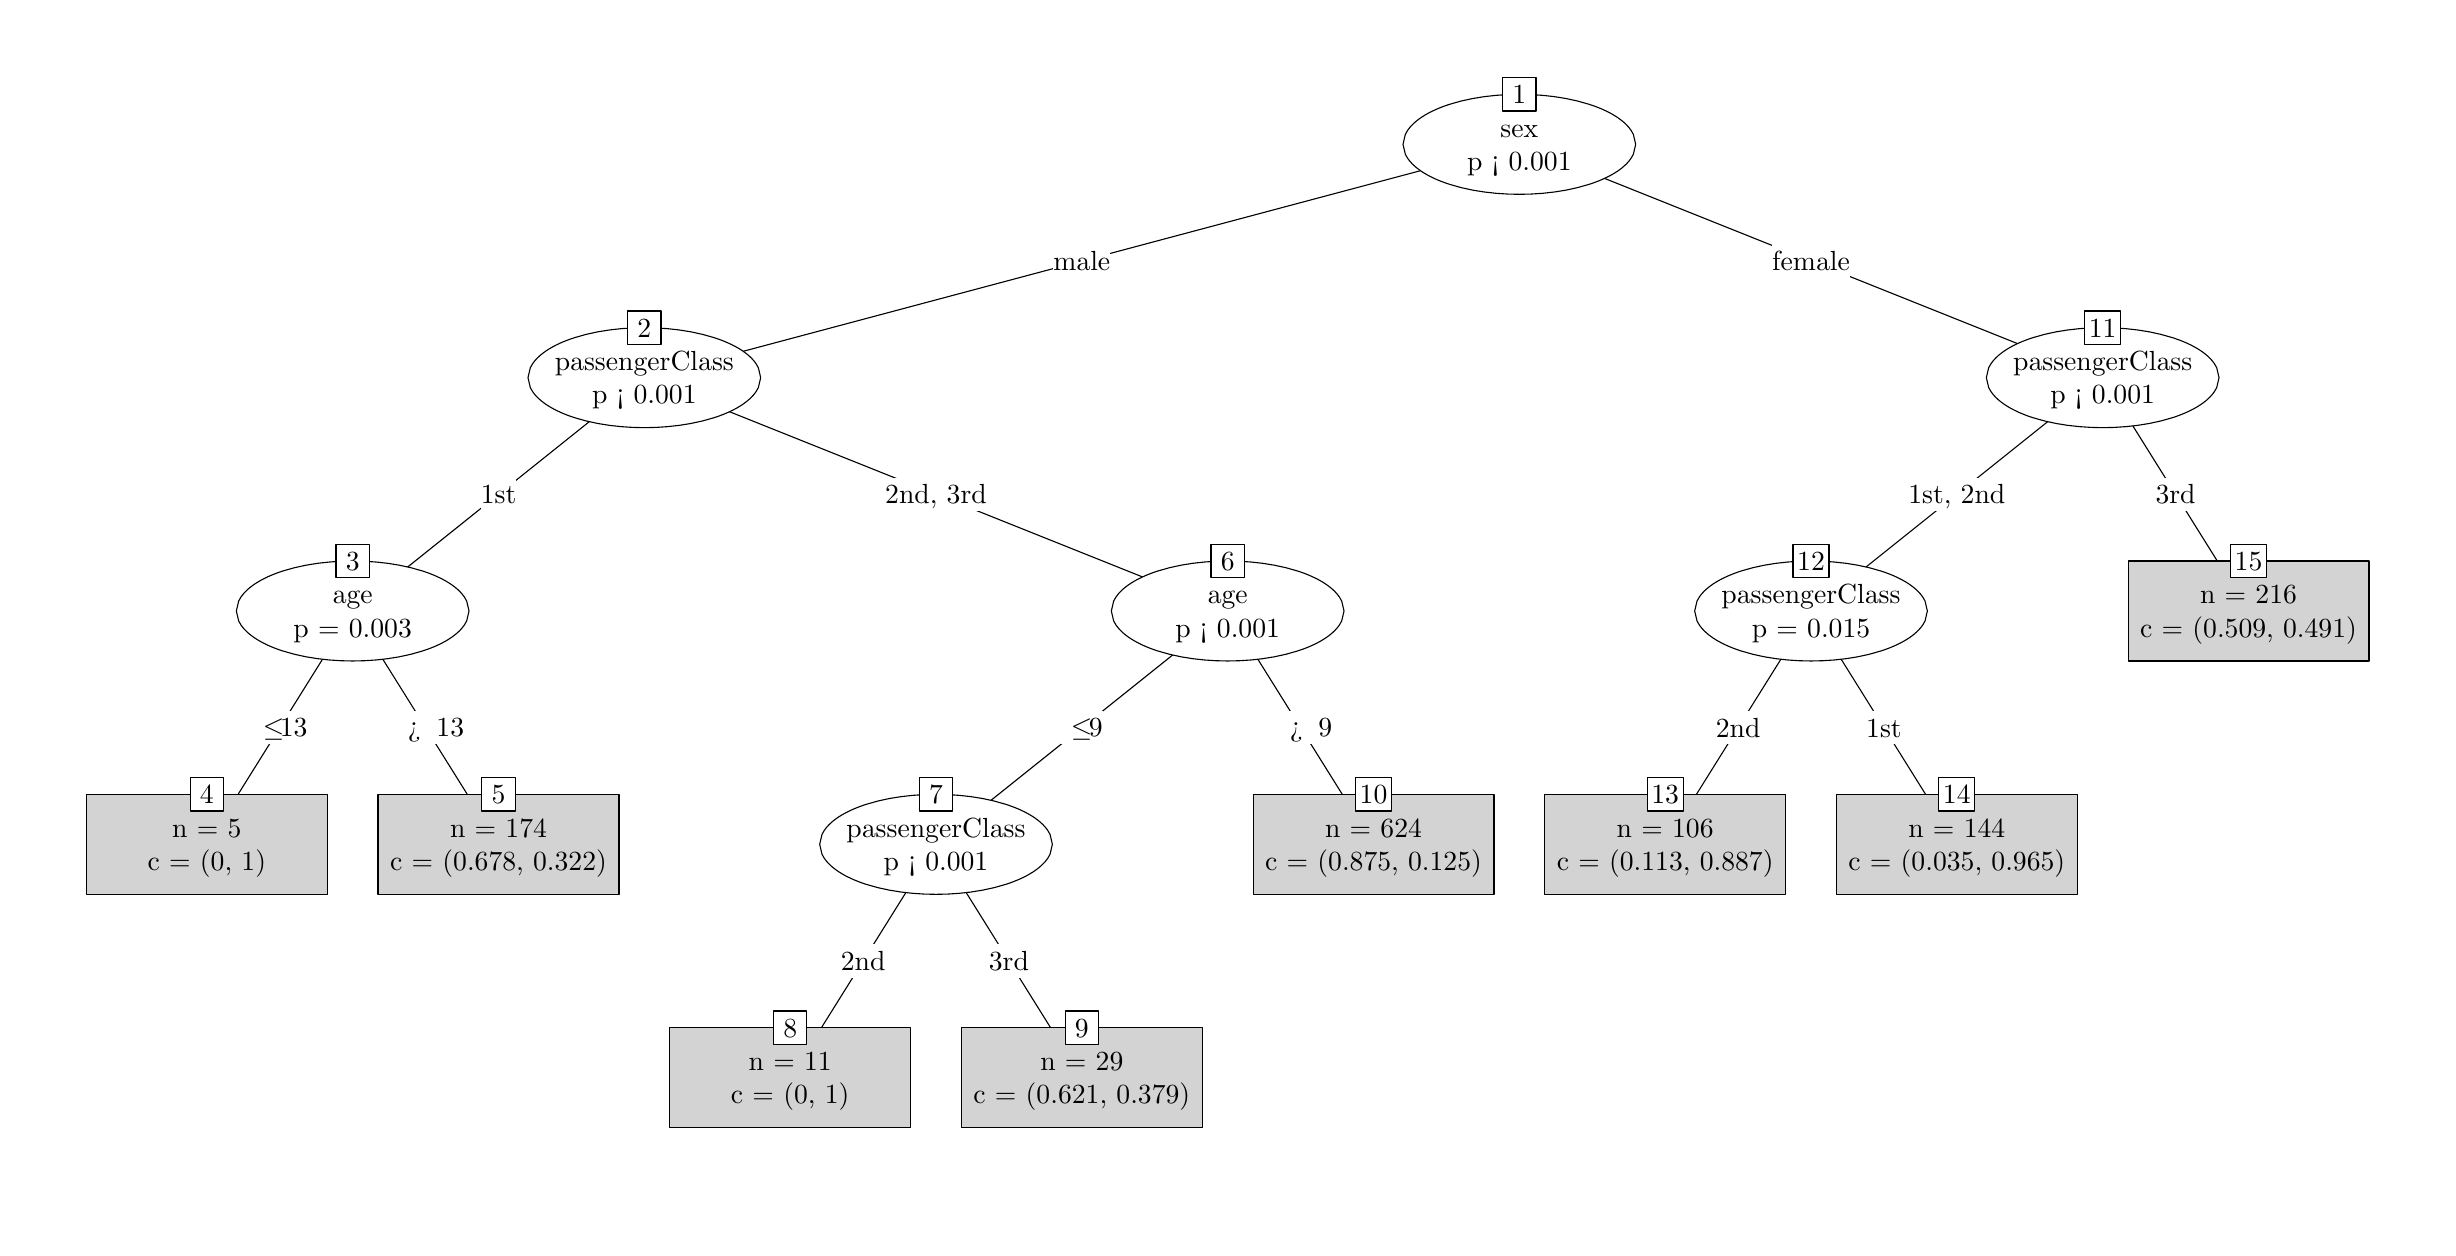
\begin{tikzpicture}[x=1pt,y=1pt]
\definecolor{fillColor}{RGB}{255,255,255}
\path[use as bounding box,fill=fillColor,fill opacity=0.00] (0,0) rectangle (867.24,433.62);
\begin{scope}
\path[clip] (  0.00,  0.00) rectangle (867.24,433.62);
\definecolor{drawColor}{RGB}{0,0,0}

\path[draw=drawColor,line width= 0.4pt,line join=round,line cap=round] (539.01,391.46) --
	(222.83,307.15);

\path[draw=drawColor,line width= 0.4pt,line join=round,line cap=round] (539.01,391.46) --
	(749.80,307.15);
\definecolor{fillColor}{RGB}{255,255,255}

\path[draw=drawColor,line width= 0.4pt,line join=round,line cap=round,fill=fillColor] (496.97,391.46) --
	(497.81,395.06) --
	(498.65,396.52) --
	(499.50,397.63) --
	(500.34,398.54) --
	(501.18,399.34) --
	(502.02,400.04) --
	(502.86,400.68) --
	(503.70,401.27) --
	(504.54,401.80) --
	(505.38,402.30) --
	(506.22,402.77) --
	(507.06,403.20) --
	(507.90,403.61) --
	(508.74,404.00) --
	(509.58,404.37) --
	(510.43,404.71) --
	(511.27,405.04) --
	(512.11,405.35) --
	(512.95,405.64) --
	(513.79,405.92) --
	(513.79,405.92) --
	(517.99,407.11) --
	(522.20,408.02) --
	(526.40,408.70) --
	(530.61,409.16) --
	(534.81,409.44) --
	(539.01,409.53) --
	(543.22,409.44) --
	(547.42,409.16) --
	(551.63,408.70) --
	(555.83,408.02) --
	(560.03,407.11) --
	(564.24,405.92) --
	(564.24,405.92) --
	(565.08,405.64) --
	(565.92,405.35) --
	(566.76,405.04) --
	(567.60,404.71) --
	(568.44,404.37) --
	(569.28,404.00) --
	(570.12,403.61) --
	(570.97,403.20) --
	(571.81,402.77) --
	(572.65,402.30) --
	(573.49,401.80) --
	(574.33,401.27) --
	(575.17,400.68) --
	(576.01,400.04) --
	(576.85,399.34) --
	(577.69,398.54) --
	(578.53,397.63) --
	(579.37,396.52) --
	(580.21,395.06) --
	(581.05,391.46) --
	(581.05,391.46) --
	(580.21,387.87) --
	(579.37,386.40) --
	(578.53,385.30) --
	(577.69,384.38) --
	(576.85,383.59) --
	(576.01,382.88) --
	(575.17,382.24) --
	(574.33,381.66) --
	(573.49,381.12) --
	(572.65,380.62) --
	(571.81,380.16) --
	(570.97,379.72) --
	(570.12,379.31) --
	(569.28,378.92) --
	(568.44,378.56) --
	(567.60,378.22) --
	(566.76,377.89) --
	(565.92,377.58) --
	(565.08,377.29) --
	(564.24,377.01) --
	(564.24,377.01) --
	(560.03,375.82) --
	(555.83,374.90) --
	(551.63,374.23) --
	(547.42,373.76) --
	(543.22,373.49) --
	(539.01,373.40) --
	(534.81,373.49) --
	(530.61,373.76) --
	(526.40,374.23) --
	(522.20,374.90) --
	(517.99,375.82) --
	(513.79,377.01) --
	(513.79,377.01) --
	(512.95,377.29) --
	(512.11,377.58) --
	(511.27,377.89) --
	(510.43,378.22) --
	(509.58,378.56) --
	(508.74,378.92) --
	(507.90,379.31) --
	(507.06,379.72) --
	(506.22,380.16) --
	(505.38,380.62) --
	(504.54,381.12) --
	(503.70,381.66) --
	(502.86,382.24) --
	(502.02,382.88) --
	(501.18,383.59) --
	(500.34,384.38) --
	(499.50,385.30) --
	(498.65,386.40) --
	(497.81,387.87) --
	(496.97,391.46) --
	cycle;

\node[text=drawColor,anchor=base,inner sep=0pt, outer sep=0pt, scale=  1.00] at (539.01,394.04) {sex};

\node[text=drawColor,anchor=base,inner sep=0pt, outer sep=0pt, scale=  1.00] at (539.01,382.00) {p < 0.001};

\path[draw=drawColor,line width= 0.4pt,line join=round,line cap=round,fill=fillColor] (532.99,403.51) rectangle (545.04,415.55);

\node[text=drawColor,anchor=base,inner sep=0pt, outer sep=0pt, scale=  1.00] at (539.01,406.09) {1};
\end{scope}
\begin{scope}
\path[clip] (  0.00,  0.00) rectangle (867.24,433.62);
\definecolor{fillColor}{RGB}{255,255,255}

\path[fill=fillColor] (370.65,343.28) rectangle (391.20,355.33);
\definecolor{drawColor}{RGB}{0,0,0}

\node[text=drawColor,anchor=base,inner sep=0pt, outer sep=0pt, scale=  1.00] at (380.92,345.86) {male};
\end{scope}
\begin{scope}
\path[clip] (  0.00,  0.00) rectangle (867.24,433.62);
\definecolor{fillColor}{RGB}{255,255,255}

\path[fill=fillColor] (630.38,343.28) rectangle (658.43,355.33);
\definecolor{drawColor}{RGB}{0,0,0}

\node[text=drawColor,anchor=base,inner sep=0pt, outer sep=0pt, scale=  1.00] at (644.41,345.86) {female};
\end{scope}
\begin{scope}
\path[clip] (  0.00,  0.00) rectangle (867.24,433.62);
\definecolor{drawColor}{RGB}{0,0,0}

\path[draw=drawColor,line width= 0.4pt,line join=round,line cap=round] (222.83,307.15) --
	(117.44,222.83);

\path[draw=drawColor,line width= 0.4pt,line join=round,line cap=round] (222.83,307.15) --
	(433.62,222.83);
\definecolor{fillColor}{RGB}{255,255,255}

\path[draw=drawColor,line width= 0.4pt,line join=round,line cap=round,fill=fillColor] (180.79,307.15) --
	(181.63,310.74) --
	(182.47,312.21) --
	(183.31,313.31) --
	(184.15,314.23) --
	(185.00,315.02) --
	(185.84,315.73) --
	(186.68,316.37) --
	(187.52,316.95) --
	(188.36,317.49) --
	(189.20,317.99) --
	(190.04,318.45) --
	(190.88,318.89) --
	(191.72,319.30) --
	(192.56,319.69) --
	(193.40,320.05) --
	(194.24,320.39) --
	(195.09,320.72) --
	(195.93,321.03) --
	(196.77,321.32) --
	(197.61,321.60) --
	(197.61,321.60) --
	(201.81,322.79) --
	(206.02,323.71) --
	(210.22,324.38) --
	(214.42,324.85) --
	(218.63,325.12) --
	(222.83,325.21) --
	(227.04,325.12) --
	(231.24,324.85) --
	(235.44,324.38) --
	(239.65,323.71) --
	(243.85,322.79) --
	(248.06,321.60) --
	(248.06,321.60) --
	(248.90,321.32) --
	(249.74,321.03) --
	(250.58,320.72) --
	(251.42,320.39) --
	(252.26,320.05) --
	(253.10,319.69) --
	(253.94,319.30) --
	(254.78,318.89) --
	(255.62,318.45) --
	(256.47,317.99) --
	(257.31,317.49) --
	(258.15,316.95) --
	(258.99,316.37) --
	(259.83,315.73) --
	(260.67,315.02) --
	(261.51,314.23) --
	(262.35,313.31) --
	(263.19,312.21) --
	(264.03,310.74) --
	(264.87,307.15) --
	(264.87,307.15) --
	(264.03,303.55) --
	(263.19,302.09) --
	(262.35,300.98) --
	(261.51,300.07) --
	(260.67,299.27) --
	(259.83,298.57) --
	(258.99,297.93) --
	(258.15,297.34) --
	(257.31,296.81) --
	(256.47,296.31) --
	(255.62,295.84) --
	(254.78,295.41) --
	(253.94,295.00) --
	(253.10,294.61) --
	(252.26,294.24) --
	(251.42,293.90) --
	(250.58,293.57) --
	(249.74,293.26) --
	(248.90,292.97) --
	(248.06,292.69) --
	(248.06,292.69) --
	(243.85,291.50) --
	(239.65,290.59) --
	(235.44,289.91) --
	(231.24,289.45) --
	(227.04,289.17) --
	(222.83,289.08) --
	(218.63,289.17) --
	(214.42,289.45) --
	(210.22,289.91) --
	(206.02,290.59) --
	(201.81,291.50) --
	(197.61,292.69) --
	(197.61,292.69) --
	(196.77,292.97) --
	(195.93,293.26) --
	(195.09,293.57) --
	(194.24,293.90) --
	(193.40,294.24) --
	(192.56,294.61) --
	(191.72,295.00) --
	(190.88,295.41) --
	(190.04,295.84) --
	(189.20,296.31) --
	(188.36,296.81) --
	(187.52,297.34) --
	(186.68,297.93) --
	(185.84,298.57) --
	(185.00,299.27) --
	(184.15,300.07) --
	(183.31,300.98) --
	(182.47,302.09) --
	(181.63,303.55) --
	(180.79,307.15) --
	cycle;

\node[text=drawColor,anchor=base,inner sep=0pt, outer sep=0pt, scale=  1.00] at (222.83,309.73) {passengerClass};

\node[text=drawColor,anchor=base,inner sep=0pt, outer sep=0pt, scale=  1.00] at (222.83,297.68) {p < 0.001};

\path[draw=drawColor,line width= 0.4pt,line join=round,line cap=round,fill=fillColor] (216.81,319.19) rectangle (228.85,331.24);

\node[text=drawColor,anchor=base,inner sep=0pt, outer sep=0pt, scale=  1.00] at (222.83,321.77) {2};
\end{scope}
\begin{scope}
\path[clip] (  0.00,  0.00) rectangle (867.24,433.62);
\definecolor{fillColor}{RGB}{255,255,255}

\path[fill=fillColor] (163.72,258.97) rectangle (176.55,271.01);
\definecolor{drawColor}{RGB}{0,0,0}

\node[text=drawColor,anchor=base,inner sep=0pt, outer sep=0pt, scale=  1.00] at (170.14,261.55) {1st};
\end{scope}
\begin{scope}
\path[clip] (  0.00,  0.00) rectangle (867.24,433.62);
\definecolor{fillColor}{RGB}{255,255,255}

\path[fill=fillColor] (309.88,258.97) rectangle (346.57,271.01);
\definecolor{drawColor}{RGB}{0,0,0}

\node[text=drawColor,anchor=base,inner sep=0pt, outer sep=0pt, scale=  1.00] at (328.23,261.55) {{2nd, 3rd}};
\end{scope}
\begin{scope}
\path[clip] (  0.00,  0.00) rectangle (867.24,433.62);
\definecolor{drawColor}{RGB}{0,0,0}

\path[draw=drawColor,line width= 0.4pt,line join=round,line cap=round] (117.44,222.83) --
	( 64.74,138.52);

\path[draw=drawColor,line width= 0.4pt,line join=round,line cap=round] (117.44,222.83) --
	(170.14,138.52);
\definecolor{fillColor}{RGB}{255,255,255}

\path[draw=drawColor,line width= 0.4pt,line join=round,line cap=round,fill=fillColor] ( 75.40,222.83) --
	( 76.24,226.43) --
	( 77.08,227.89) --
	( 77.92,229.00) --
	( 78.76,229.91) --
	( 79.60,230.71) --
	( 80.44,231.41) --
	( 81.28,232.05) --
	( 82.12,232.64) --
	( 82.97,233.17) --
	( 83.81,233.67) --
	( 84.65,234.14) --
	( 85.49,234.57) --
	( 86.33,234.98) --
	( 87.17,235.37) --
	( 88.01,235.74) --
	( 88.85,236.08) --
	( 89.69,236.41) --
	( 90.53,236.72) --
	( 91.37,237.01) --
	( 92.21,237.29) --
	( 92.21,237.29) --
	( 96.42,238.48) --
	(100.62,239.39) --
	(104.83,240.07) --
	(109.03,240.53) --
	(113.23,240.81) --
	(117.44,240.90) --
	(121.64,240.81) --
	(125.85,240.53) --
	(130.05,240.07) --
	(134.26,239.39) --
	(138.46,238.48) --
	(142.66,237.29) --
	(142.66,237.29) --
	(143.50,237.01) --
	(144.35,236.72) --
	(145.19,236.41) --
	(146.03,236.08) --
	(146.87,235.74) --
	(147.71,235.37) --
	(148.55,234.98) --
	(149.39,234.57) --
	(150.23,234.14) --
	(151.07,233.67) --
	(151.91,233.17) --
	(152.75,232.64) --
	(153.59,232.05) --
	(154.43,231.41) --
	(155.28,230.71) --
	(156.12,229.91) --
	(156.96,229.00) --
	(157.80,227.89) --
	(158.64,226.43) --
	(159.48,222.83) --
	(159.48,222.83) --
	(158.64,219.24) --
	(157.80,217.77) --
	(156.96,216.67) --
	(156.12,215.75) --
	(155.28,214.96) --
	(154.43,214.25) --
	(153.59,213.61) --
	(152.75,213.03) --
	(151.91,212.49) --
	(151.07,211.99) --
	(150.23,211.53) --
	(149.39,211.09) --
	(148.55,210.68) --
	(147.71,210.29) --
	(146.87,209.93) --
	(146.03,209.59) --
	(145.19,209.26) --
	(144.35,208.95) --
	(143.50,208.66) --
	(142.66,208.38) --
	(142.66,208.38) --
	(138.46,207.19) --
	(134.26,206.27) --
	(130.05,205.60) --
	(125.85,205.13) --
	(121.64,204.86) --
	(117.44,204.77) --
	(113.23,204.86) --
	(109.03,205.13) --
	(104.83,205.60) --
	(100.62,206.27) --
	( 96.42,207.19) --
	( 92.21,208.38) --
	( 92.21,208.38) --
	( 91.37,208.66) --
	( 90.53,208.95) --
	( 89.69,209.26) --
	( 88.85,209.59) --
	( 88.01,209.93) --
	( 87.17,210.29) --
	( 86.33,210.68) --
	( 85.49,211.09) --
	( 84.65,211.53) --
	( 83.81,211.99) --
	( 82.97,212.49) --
	( 82.12,213.03) --
	( 81.28,213.61) --
	( 80.44,214.25) --
	( 79.60,214.96) --
	( 78.76,215.75) --
	( 77.92,216.67) --
	( 77.08,217.77) --
	( 76.24,219.24) --
	( 75.40,222.83) --
	cycle;

\node[text=drawColor,anchor=base,inner sep=0pt, outer sep=0pt, scale=  1.00] at (117.44,225.41) {age};

\node[text=drawColor,anchor=base,inner sep=0pt, outer sep=0pt, scale=  1.00] at (117.44,213.37) {p = 0.003};

\path[draw=drawColor,line width= 0.4pt,line join=round,line cap=round,fill=fillColor] (111.42,234.88) rectangle (123.46,246.92);

\node[text=drawColor,anchor=base,inner sep=0pt, outer sep=0pt, scale=  1.00] at (117.44,237.46) {3};
\end{scope}
\begin{scope}
\path[clip] (  0.00,  0.00) rectangle (867.24,433.62);
\definecolor{fillColor}{RGB}{255,255,255}

\path[fill=fillColor] ( 81.05,174.65) rectangle (101.13,186.70);
\definecolor{drawColor}{RGB}{0,0,0}

\node[text=drawColor,anchor=base west,inner sep=0pt, outer sep=0pt, scale=  1.00] at ( 85.0,177.47) {$\leq$};

\node[text=drawColor,anchor=base west,inner sep=0pt, outer sep=0pt, scale=  1.00] at ( 91.14,177.47) {13};
\end{scope}
\begin{scope}
\path[clip] (  0.00,  0.00) rectangle (867.24,433.62);
\definecolor{fillColor}{RGB}{255,255,255}

\path[fill=fillColor] (129.86,174.65) rectangle (157.72,186.70);
\definecolor{drawColor}{RGB}{0,0,0}

\node[text=drawColor,anchor=base west,inner sep=0pt, outer sep=0pt, scale=  1.00] at (137.40,177.66) {>};

\node[text=drawColor,anchor=base west,inner sep=0pt, outer sep=0pt, scale=  1.00] at (147.72,177.66) {13};
\end{scope}
\begin{scope}
\path[clip] (  0.00,  0.00) rectangle (867.24,433.62);
\definecolor{drawColor}{RGB}{0,0,0}
\definecolor{fillColor}{RGB}{211,211,211}

\path[draw=drawColor,line width= 0.4pt,line join=round,line cap=round,fill=fillColor] ( 21.21,120.45) rectangle (108.27,156.59);

\node[text=drawColor,anchor=base,inner sep=0pt, outer sep=0pt, scale=  1.00] at ( 64.74,141.10) {n = 5};

\node[text=drawColor,anchor=base,inner sep=0pt, outer sep=0pt, scale=  1.00] at ( 64.74,129.05) {c = (0, 1)};
\definecolor{fillColor}{RGB}{255,255,255}

\path[draw=drawColor,line width= 0.4pt,line join=round,line cap=round,fill=fillColor] ( 58.72,150.56) rectangle ( 70.76,162.61);

\node[text=drawColor,anchor=base,inner sep=0pt, outer sep=0pt, scale=  1.00] at ( 64.74,153.14) {4};
\end{scope}
\begin{scope}
\path[clip] (  0.00,  0.00) rectangle (867.24,433.62);
\definecolor{drawColor}{RGB}{0,0,0}
\definecolor{fillColor}{RGB}{211,211,211}

\path[draw=drawColor,line width= 0.4pt,line join=round,line cap=round,fill=fillColor] (126.60,120.45) rectangle (213.67,156.59);

\node[text=drawColor,anchor=base,inner sep=0pt, outer sep=0pt, scale=  1.00] at (170.14,141.10) {n = 174};

\node[text=drawColor,anchor=base,inner sep=0pt, outer sep=0pt, scale=  1.00] at (170.14,129.05) {c = (0.678, 0.322)};
\definecolor{fillColor}{RGB}{255,255,255}

\path[draw=drawColor,line width= 0.4pt,line join=round,line cap=round,fill=fillColor] (164.11,150.56) rectangle (176.16,162.61);

\node[text=drawColor,anchor=base,inner sep=0pt, outer sep=0pt, scale=  1.00] at (170.14,153.14) {5};
\end{scope}
\begin{scope}
\path[clip] (  0.00,  0.00) rectangle (867.24,433.62);
\definecolor{drawColor}{RGB}{0,0,0}

\path[draw=drawColor,line width= 0.4pt,line join=round,line cap=round] (433.62,222.83) --
	(328.23,138.52);

\path[draw=drawColor,line width= 0.4pt,line join=round,line cap=round] (433.62,222.83) --
	(486.32,138.52);
\definecolor{fillColor}{RGB}{255,255,255}

\path[draw=drawColor,line width= 0.4pt,line join=round,line cap=round,fill=fillColor] (391.58,222.83) --
	(392.42,226.43) --
	(393.26,227.89) --
	(394.10,229.00) --
	(394.94,229.91) --
	(395.78,230.71) --
	(396.62,231.41) --
	(397.46,232.05) --
	(398.31,232.64) --
	(399.15,233.17) --
	(399.99,233.67) --
	(400.83,234.14) --
	(401.67,234.57) --
	(402.51,234.98) --
	(403.35,235.37) --
	(404.19,235.74) --
	(405.03,236.08) --
	(405.87,236.41) --
	(406.71,236.72) --
	(407.55,237.01) --
	(408.40,237.29) --
	(408.40,237.29) --
	(412.60,238.48) --
	(416.80,239.39) --
	(421.01,240.07) --
	(425.21,240.53) --
	(429.42,240.81) --
	(433.62,240.90) --
	(437.82,240.81) --
	(442.03,240.53) --
	(446.23,240.07) --
	(450.44,239.39) --
	(454.64,238.48) --
	(458.84,237.29) --
	(458.84,237.29) --
	(459.69,237.01) --
	(460.53,236.72) --
	(461.37,236.41) --
	(462.21,236.08) --
	(463.05,235.74) --
	(463.89,235.37) --
	(464.73,234.98) --
	(465.57,234.57) --
	(466.41,234.14) --
	(467.25,233.67) --
	(468.09,233.17) --
	(468.93,232.64) --
	(469.78,232.05) --
	(470.62,231.41) --
	(471.46,230.71) --
	(472.30,229.91) --
	(473.14,229.00) --
	(473.98,227.89) --
	(474.82,226.43) --
	(475.66,222.83) --
	(475.66,222.83) --
	(474.82,219.24) --
	(473.98,217.77) --
	(473.14,216.67) --
	(472.30,215.75) --
	(471.46,214.96) --
	(470.62,214.25) --
	(469.78,213.61) --
	(468.93,213.03) --
	(468.09,212.49) --
	(467.25,211.99) --
	(466.41,211.53) --
	(465.57,211.09) --
	(464.73,210.68) --
	(463.89,210.29) --
	(463.05,209.93) --
	(462.21,209.59) --
	(461.37,209.26) --
	(460.53,208.95) --
	(459.69,208.66) --
	(458.84,208.38) --
	(458.84,208.38) --
	(454.64,207.19) --
	(450.44,206.27) --
	(446.23,205.60) --
	(442.03,205.13) --
	(437.82,204.86) --
	(433.62,204.77) --
	(429.42,204.86) --
	(425.21,205.13) --
	(421.01,205.60) --
	(416.80,206.27) --
	(412.60,207.19) --
	(408.40,208.38) --
	(408.40,208.38) --
	(407.55,208.66) --
	(406.71,208.95) --
	(405.87,209.26) --
	(405.03,209.59) --
	(404.19,209.93) --
	(403.35,210.29) --
	(402.51,210.68) --
	(401.67,211.09) --
	(400.83,211.53) --
	(399.99,211.99) --
	(399.15,212.49) --
	(398.31,213.03) --
	(397.46,213.61) --
	(396.62,214.25) --
	(395.78,214.96) --
	(394.94,215.75) --
	(394.10,216.67) --
	(393.26,217.77) --
	(392.42,219.24) --
	(391.58,222.83) --
	cycle;

\node[text=drawColor,anchor=base,inner sep=0pt, outer sep=0pt, scale=  1.00] at (433.62,225.41) {age};

\node[text=drawColor,anchor=base,inner sep=0pt, outer sep=0pt, scale=  1.00] at (433.62,213.37) {p < 0.001};

\path[draw=drawColor,line width= 0.4pt,line join=round,line cap=round,fill=fillColor] (427.60,234.88) rectangle (439.64,246.92);

\node[text=drawColor,anchor=base,inner sep=0pt, outer sep=0pt, scale=  1.00] at (433.62,237.46) {6};
\end{scope}
\begin{scope}
\path[clip] (  0.00,  0.00) rectangle (867.24,433.62);
\definecolor{fillColor}{RGB}{255,255,255}

\path[fill=fillColor] (373.38,174.65) rectangle (388.47,186.70);
\definecolor{drawColor}{RGB}{0,0,0}

\node[text=drawColor,anchor=base west,inner sep=0pt, outer sep=0pt, scale=  1.00] at (377.0,177.47) {$\leq$};

\node[text=drawColor,anchor=base west,inner sep=0pt, outer sep=0pt, scale=  1.00] at (383.47,177.47) {9};
\end{scope}
\begin{scope}
\path[clip] (  0.00,  0.00) rectangle (867.24,433.62);
\definecolor{fillColor}{RGB}{255,255,255}

\path[fill=fillColor] (448.54,174.65) rectangle (471.40,186.70);
\definecolor{drawColor}{RGB}{0,0,0}

\node[text=drawColor,anchor=base west,inner sep=0pt, outer sep=0pt, scale=  1.00] at (456.08,177.66) {>};

\node[text=drawColor,anchor=base west,inner sep=0pt, outer sep=0pt, scale=  1.00] at (466.40,177.66) {9};
\end{scope}
\begin{scope}
\path[clip] (  0.00,  0.00) rectangle (867.24,433.62);
\definecolor{drawColor}{RGB}{0,0,0}

\path[draw=drawColor,line width= 0.4pt,line join=round,line cap=round] (328.23,138.52) --
	(275.53, 54.20);

\path[draw=drawColor,line width= 0.4pt,line join=round,line cap=round] (328.23,138.52) --
	(380.92, 54.20);
\definecolor{fillColor}{RGB}{255,255,255}

\path[draw=drawColor,line width= 0.4pt,line join=round,line cap=round,fill=fillColor] (286.19,138.52) --
	(287.03,142.11) --
	(287.87,143.58) --
	(288.71,144.68) --
	(289.55,145.60) --
	(290.39,146.39) --
	(291.23,147.10) --
	(292.07,147.74) --
	(292.91,148.32) --
	(293.75,148.86) --
	(294.59,149.36) --
	(295.43,149.82) --
	(296.27,150.26) --
	(297.12,150.67) --
	(297.96,151.06) --
	(298.80,151.42) --
	(299.64,151.76) --
	(300.48,152.09) --
	(301.32,152.40) --
	(302.16,152.69) --
	(303.00,152.97) --
	(303.00,152.97) --
	(307.21,154.16) --
	(311.41,155.08) --
	(315.61,155.75) --
	(319.82,156.22) --
	(324.02,156.49) --
	(328.23,156.58) --
	(332.43,156.49) --
	(336.63,156.22) --
	(340.84,155.75) --
	(345.04,155.08) --
	(349.25,154.16) --
	(353.45,152.97) --
	(353.45,152.97) --
	(354.29,152.69) --
	(355.13,152.40) --
	(355.97,152.09) --
	(356.81,151.76) --
	(357.66,151.42) --
	(358.50,151.06) --
	(359.34,150.67) --
	(360.18,150.26) --
	(361.02,149.82) --
	(361.86,149.36) --
	(362.70,148.86) --
	(363.54,148.32) --
	(364.38,147.74) --
	(365.22,147.10) --
	(366.06,146.39) --
	(366.90,145.60) --
	(367.74,144.68) --
	(368.59,143.58) --
	(369.43,142.11) --
	(370.27,138.52) --
	(370.27,138.52) --
	(369.43,134.92) --
	(368.59,133.46) --
	(367.74,132.35) --
	(366.90,131.44) --
	(366.06,130.64) --
	(365.22,129.94) --
	(364.38,129.30) --
	(363.54,128.71) --
	(362.70,128.18) --
	(361.86,127.68) --
	(361.02,127.21) --
	(360.18,126.78) --
	(359.34,126.37) --
	(358.50,125.98) --
	(357.66,125.61) --
	(356.81,125.27) --
	(355.97,124.94) --
	(355.13,124.63) --
	(354.29,124.34) --
	(353.45,124.06) --
	(353.45,124.06) --
	(349.25,122.87) --
	(345.04,121.96) --
	(340.84,121.28) --
	(336.63,120.82) --
	(332.43,120.54) --
	(328.23,120.45) --
	(324.02,120.54) --
	(319.82,120.82) --
	(315.61,121.28) --
	(311.41,121.96) --
	(307.21,122.87) --
	(303.00,124.06) --
	(303.00,124.06) --
	(302.16,124.34) --
	(301.32,124.63) --
	(300.48,124.94) --
	(299.64,125.27) --
	(298.80,125.61) --
	(297.96,125.98) --
	(297.12,126.37) --
	(296.27,126.78) --
	(295.43,127.21) --
	(294.59,127.68) --
	(293.75,128.18) --
	(292.91,128.71) --
	(292.07,129.30) --
	(291.23,129.94) --
	(290.39,130.64) --
	(289.55,131.44) --
	(288.71,132.35) --
	(287.87,133.46) --
	(287.03,134.92) --
	(286.19,138.52) --
	cycle;

\node[text=drawColor,anchor=base,inner sep=0pt, outer sep=0pt, scale=  1.00] at (328.23,141.10) {passengerClass};

\node[text=drawColor,anchor=base,inner sep=0pt, outer sep=0pt, scale=  1.00] at (328.23,129.05) {p < 0.001};

\path[draw=drawColor,line width= 0.4pt,line join=round,line cap=round,fill=fillColor] (322.20,150.56) rectangle (334.25,162.61);

\node[text=drawColor,anchor=base,inner sep=0pt, outer sep=0pt, scale=  1.00] at (328.23,153.14) {7};
\end{scope}
\begin{scope}
\path[clip] (  0.00,  0.00) rectangle (867.24,433.62);
\definecolor{fillColor}{RGB}{255,255,255}

\path[fill=fillColor] (293.82, 90.34) rectangle (309.93,102.38);
\definecolor{drawColor}{RGB}{0,0,0}

\node[text=drawColor,anchor=base,inner sep=0pt, outer sep=0pt, scale=  1.00] at (301.88, 92.92) {2nd};
\end{scope}
\begin{scope}
\path[clip] (  0.00,  0.00) rectangle (867.24,433.62);
\definecolor{fillColor}{RGB}{255,255,255}

\path[fill=fillColor] (347.34, 90.34) rectangle (361.81,102.38);
\definecolor{drawColor}{RGB}{0,0,0}

\node[text=drawColor,anchor=base,inner sep=0pt, outer sep=0pt, scale=  1.00] at (354.57, 92.92) {3rd};
\end{scope}
\begin{scope}
\path[clip] (  0.00,  0.00) rectangle (867.24,433.62);
\definecolor{drawColor}{RGB}{0,0,0}
\definecolor{fillColor}{RGB}{211,211,211}

\path[draw=drawColor,line width= 0.4pt,line join=round,line cap=round,fill=fillColor] (232.00, 36.14) rectangle (319.06, 72.27);

\node[text=drawColor,anchor=base,inner sep=0pt, outer sep=0pt, scale=  1.00] at (275.53, 56.78) {n = 11};

\node[text=drawColor,anchor=base,inner sep=0pt, outer sep=0pt, scale=  1.00] at (275.53, 44.74) {c = (0, 1)};
\definecolor{fillColor}{RGB}{255,255,255}

\path[draw=drawColor,line width= 0.4pt,line join=round,line cap=round,fill=fillColor] (269.51, 66.25) rectangle (281.55, 78.29);

\node[text=drawColor,anchor=base,inner sep=0pt, outer sep=0pt, scale=  1.00] at (275.53, 68.83) {8};
\end{scope}
\begin{scope}
\path[clip] (  0.00,  0.00) rectangle (867.24,433.62);
\definecolor{drawColor}{RGB}{0,0,0}
\definecolor{fillColor}{RGB}{211,211,211}

\path[draw=drawColor,line width= 0.4pt,line join=round,line cap=round,fill=fillColor] (337.39, 36.14) rectangle (424.45, 72.27);

\node[text=drawColor,anchor=base,inner sep=0pt, outer sep=0pt, scale=  1.00] at (380.92, 56.78) {n = 29};

\node[text=drawColor,anchor=base,inner sep=0pt, outer sep=0pt, scale=  1.00] at (380.92, 44.74) {c = (0.621, 0.379)};
\definecolor{fillColor}{RGB}{255,255,255}

\path[draw=drawColor,line width= 0.4pt,line join=round,line cap=round,fill=fillColor] (374.90, 66.25) rectangle (386.95, 78.29);

\node[text=drawColor,anchor=base,inner sep=0pt, outer sep=0pt, scale=  1.00] at (380.92, 68.83) {9};
\end{scope}
\begin{scope}
\path[clip] (  0.00,  0.00) rectangle (867.24,433.62);
\definecolor{drawColor}{RGB}{0,0,0}
\definecolor{fillColor}{RGB}{211,211,211}

\path[draw=drawColor,line width= 0.4pt,line join=round,line cap=round,fill=fillColor] (442.79,120.45) rectangle (529.85,156.59);

\node[text=drawColor,anchor=base,inner sep=0pt, outer sep=0pt, scale=  1.00] at (486.32,141.10) {n = 624};

\node[text=drawColor,anchor=base,inner sep=0pt, outer sep=0pt, scale=  1.00] at (486.32,129.05) {c = (0.875, 0.125)};
\definecolor{fillColor}{RGB}{255,255,255}

\path[draw=drawColor,line width= 0.4pt,line join=round,line cap=round,fill=fillColor] (479.82,150.56) rectangle (492.82,162.61);

\node[text=drawColor,anchor=base,inner sep=0pt, outer sep=0pt, scale=  1.00] at (486.32,153.14) {10};
\end{scope}
\begin{scope}
\path[clip] (  0.00,  0.00) rectangle (867.24,433.62);
\definecolor{drawColor}{RGB}{0,0,0}

\path[draw=drawColor,line width= 0.4pt,line join=round,line cap=round] (749.80,307.15) --
	(644.41,222.83);

\path[draw=drawColor,line width= 0.4pt,line join=round,line cap=round] (749.80,307.15) --
	(802.50,222.83);
\definecolor{fillColor}{RGB}{255,255,255}

\path[draw=drawColor,line width= 0.4pt,line join=round,line cap=round,fill=fillColor] (707.76,307.15) --
	(708.60,310.74) --
	(709.44,312.21) --
	(710.28,313.31) --
	(711.12,314.23) --
	(711.96,315.02) --
	(712.81,315.73) --
	(713.65,316.37) --
	(714.49,316.95) --
	(715.33,317.49) --
	(716.17,317.99) --
	(717.01,318.45) --
	(717.85,318.89) --
	(718.69,319.30) --
	(719.53,319.69) --
	(720.37,320.05) --
	(721.21,320.39) --
	(722.05,320.72) --
	(722.89,321.03) --
	(723.74,321.32) --
	(724.58,321.60) --
	(724.58,321.60) --
	(728.78,322.79) --
	(732.98,323.71) --
	(737.19,324.38) --
	(741.39,324.85) --
	(745.60,325.12) --
	(749.80,325.21) --
	(754.01,325.12) --
	(758.21,324.85) --
	(762.41,324.38) --
	(766.62,323.71) --
	(770.82,322.79) --
	(775.03,321.60) --
	(775.03,321.60) --
	(775.87,321.32) --
	(776.71,321.03) --
	(777.55,320.72) --
	(778.39,320.39) --
	(779.23,320.05) --
	(780.07,319.69) --
	(780.91,319.30) --
	(781.75,318.89) --
	(782.59,318.45) --
	(783.43,317.99) --
	(784.27,317.49) --
	(785.12,316.95) --
	(785.96,316.37) --
	(786.80,315.73) --
	(787.64,315.02) --
	(788.48,314.23) --
	(789.32,313.31) --
	(790.16,312.21) --
	(791.00,310.74) --
	(791.84,307.15) --
	(791.84,307.15) --
	(791.00,303.55) --
	(790.16,302.09) --
	(789.32,300.98) --
	(788.48,300.07) --
	(787.64,299.27) --
	(786.80,298.57) --
	(785.96,297.93) --
	(785.12,297.34) --
	(784.27,296.81) --
	(783.43,296.31) --
	(782.59,295.84) --
	(781.75,295.41) --
	(780.91,295.00) --
	(780.07,294.61) --
	(779.23,294.24) --
	(778.39,293.90) --
	(777.55,293.57) --
	(776.71,293.26) --
	(775.87,292.97) --
	(775.03,292.69) --
	(775.03,292.69) --
	(770.82,291.50) --
	(766.62,290.59) --
	(762.41,289.91) --
	(758.21,289.45) --
	(754.01,289.17) --
	(749.80,289.08) --
	(745.60,289.17) --
	(741.39,289.45) --
	(737.19,289.91) --
	(732.98,290.59) --
	(728.78,291.50) --
	(724.58,292.69) --
	(724.58,292.69) --
	(723.74,292.97) --
	(722.89,293.26) --
	(722.05,293.57) --
	(721.21,293.90) --
	(720.37,294.24) --
	(719.53,294.61) --
	(718.69,295.00) --
	(717.85,295.41) --
	(717.01,295.84) --
	(716.17,296.31) --
	(715.33,296.81) --
	(714.49,297.34) --
	(713.65,297.93) --
	(712.81,298.57) --
	(711.96,299.27) --
	(711.12,300.07) --
	(710.28,300.98) --
	(709.44,302.09) --
	(708.60,303.55) --
	(707.76,307.15) --
	cycle;

\node[text=drawColor,anchor=base,inner sep=0pt, outer sep=0pt, scale=  1.00] at (749.80,309.73) {passengerClass};

\node[text=drawColor,anchor=base,inner sep=0pt, outer sep=0pt, scale=  1.00] at (749.80,297.68) {p < 0.001};

\path[draw=drawColor,line width= 0.4pt,line join=round,line cap=round,fill=fillColor] (743.30,319.19) rectangle (756.30,331.24);

\node[text=drawColor,anchor=base,inner sep=0pt, outer sep=0pt, scale=  1.00] at (749.80,321.77) {11};
\end{scope}
\begin{scope}
\path[clip] (  0.00,  0.00) rectangle (867.24,433.62);
\definecolor{fillColor}{RGB}{255,255,255}

\path[fill=fillColor] (679.58,258.97) rectangle (714.63,271.01);
\definecolor{drawColor}{RGB}{0,0,0}

\node[text=drawColor,anchor=base,inner sep=0pt, outer sep=0pt, scale=  1.00] at (697.10,261.55) {{1st, 2nd}};
\end{scope}
\begin{scope}
\path[clip] (  0.00,  0.00) rectangle (867.24,433.62);
\definecolor{fillColor}{RGB}{255,255,255}

\path[fill=fillColor] (768.92,258.97) rectangle (783.38,271.01);
\definecolor{drawColor}{RGB}{0,0,0}

\node[text=drawColor,anchor=base,inner sep=0pt, outer sep=0pt, scale=  1.00] at (776.15,261.55) {3rd};
\end{scope}
\begin{scope}
\path[clip] (  0.00,  0.00) rectangle (867.24,433.62);
\definecolor{drawColor}{RGB}{0,0,0}

\path[draw=drawColor,line width= 0.4pt,line join=round,line cap=round] (644.41,222.83) --
	(591.71,138.52);

\path[draw=drawColor,line width= 0.4pt,line join=round,line cap=round] (644.41,222.83) --
	(697.10,138.52);
\definecolor{fillColor}{RGB}{255,255,255}

\path[draw=drawColor,line width= 0.4pt,line join=round,line cap=round,fill=fillColor] (602.37,222.83) --
	(603.21,226.43) --
	(604.05,227.89) --
	(604.89,229.00) --
	(605.73,229.91) --
	(606.57,230.71) --
	(607.41,231.41) --
	(608.25,232.05) --
	(609.09,232.64) --
	(609.93,233.17) --
	(610.77,233.67) --
	(611.62,234.14) --
	(612.46,234.57) --
	(613.30,234.98) --
	(614.14,235.37) --
	(614.98,235.74) --
	(615.82,236.08) --
	(616.66,236.41) --
	(617.50,236.72) --
	(618.34,237.01) --
	(619.18,237.29) --
	(619.18,237.29) --
	(623.39,238.48) --
	(627.59,239.39) --
	(631.80,240.07) --
	(636.00,240.53) --
	(640.20,240.81) --
	(644.41,240.90) --
	(648.61,240.81) --
	(652.82,240.53) --
	(657.02,240.07) --
	(661.22,239.39) --
	(665.43,238.48) --
	(669.63,237.29) --
	(669.63,237.29) --
	(670.47,237.01) --
	(671.31,236.72) --
	(672.15,236.41) --
	(673.00,236.08) --
	(673.84,235.74) --
	(674.68,235.37) --
	(675.52,234.98) --
	(676.36,234.57) --
	(677.20,234.14) --
	(678.04,233.67) --
	(678.88,233.17) --
	(679.72,232.64) --
	(680.56,232.05) --
	(681.40,231.41) --
	(682.24,230.71) --
	(683.09,229.91) --
	(683.93,229.00) --
	(684.77,227.89) --
	(685.61,226.43) --
	(686.45,222.83) --
	(686.45,222.83) --
	(685.61,219.24) --
	(684.77,217.77) --
	(683.93,216.67) --
	(683.09,215.75) --
	(682.24,214.96) --
	(681.40,214.25) --
	(680.56,213.61) --
	(679.72,213.03) --
	(678.88,212.49) --
	(678.04,211.99) --
	(677.20,211.53) --
	(676.36,211.09) --
	(675.52,210.68) --
	(674.68,210.29) --
	(673.84,209.93) --
	(673.00,209.59) --
	(672.15,209.26) --
	(671.31,208.95) --
	(670.47,208.66) --
	(669.63,208.38) --
	(669.63,208.38) --
	(665.43,207.19) --
	(661.22,206.27) --
	(657.02,205.60) --
	(652.82,205.13) --
	(648.61,204.86) --
	(644.41,204.77) --
	(640.20,204.86) --
	(636.00,205.13) --
	(631.80,205.60) --
	(627.59,206.27) --
	(623.39,207.19) --
	(619.18,208.38) --
	(619.18,208.38) --
	(618.34,208.66) --
	(617.50,208.95) --
	(616.66,209.26) --
	(615.82,209.59) --
	(614.98,209.93) --
	(614.14,210.29) --
	(613.30,210.68) --
	(612.46,211.09) --
	(611.62,211.53) --
	(610.77,211.99) --
	(609.93,212.49) --
	(609.09,213.03) --
	(608.25,213.61) --
	(607.41,214.25) --
	(606.57,214.96) --
	(605.73,215.75) --
	(604.89,216.67) --
	(604.05,217.77) --
	(603.21,219.24) --
	(602.37,222.83) --
	cycle;

\node[text=drawColor,anchor=base,inner sep=0pt, outer sep=0pt, scale=  1.00] at (644.41,225.41) {passengerClass};

\node[text=drawColor,anchor=base,inner sep=0pt, outer sep=0pt, scale=  1.00] at (644.41,213.37) {p = 0.015};

\path[draw=drawColor,line width= 0.4pt,line join=round,line cap=round,fill=fillColor] (637.91,234.88) rectangle (650.91,246.92);

\node[text=drawColor,anchor=base,inner sep=0pt, outer sep=0pt, scale=  1.00] at (644.41,237.46) {12};
\end{scope}
\begin{scope}
\path[clip] (  0.00,  0.00) rectangle (867.24,433.62);
\definecolor{fillColor}{RGB}{255,255,255}

\path[fill=fillColor] (610.01,174.65) rectangle (626.11,186.70);
\definecolor{drawColor}{RGB}{0,0,0}

\node[text=drawColor,anchor=base,inner sep=0pt, outer sep=0pt, scale=  1.00] at (618.06,177.23) {2nd};
\end{scope}
\begin{scope}
\path[clip] (  0.00,  0.00) rectangle (867.24,433.62);
\definecolor{fillColor}{RGB}{255,255,255}

\path[fill=fillColor] (664.34,174.65) rectangle (677.17,186.70);
\definecolor{drawColor}{RGB}{0,0,0}

\node[text=drawColor,anchor=base,inner sep=0pt, outer sep=0pt, scale=  1.00] at (670.76,177.23) {1st};
\end{scope}
\begin{scope}
\path[clip] (  0.00,  0.00) rectangle (867.24,433.62);
\definecolor{drawColor}{RGB}{0,0,0}
\definecolor{fillColor}{RGB}{211,211,211}

\path[draw=drawColor,line width= 0.4pt,line join=round,line cap=round,fill=fillColor] (548.18,120.45) rectangle (635.24,156.59);

\node[text=drawColor,anchor=base,inner sep=0pt, outer sep=0pt, scale=  1.00] at (591.71,141.10) {n = 106};

\node[text=drawColor,anchor=base,inner sep=0pt, outer sep=0pt, scale=  1.00] at (591.71,129.05) {c = (0.113, 0.887)};
\definecolor{fillColor}{RGB}{255,255,255}

\path[draw=drawColor,line width= 0.4pt,line join=round,line cap=round,fill=fillColor] (585.21,150.56) rectangle (598.21,162.61);

\node[text=drawColor,anchor=base,inner sep=0pt, outer sep=0pt, scale=  1.00] at (591.71,153.14) {13};
\end{scope}
\begin{scope}
\path[clip] (  0.00,  0.00) rectangle (867.24,433.62);
\definecolor{drawColor}{RGB}{0,0,0}
\definecolor{fillColor}{RGB}{211,211,211}

\path[draw=drawColor,line width= 0.4pt,line join=round,line cap=round,fill=fillColor] (653.57,120.45) rectangle (740.64,156.59);

\node[text=drawColor,anchor=base,inner sep=0pt, outer sep=0pt, scale=  1.00] at (697.10,141.10) {n = 144};

\node[text=drawColor,anchor=base,inner sep=0pt, outer sep=0pt, scale=  1.00] at (697.10,129.05) {c = (0.035, 0.965)};
\definecolor{fillColor}{RGB}{255,255,255}

\path[draw=drawColor,line width= 0.4pt,line join=round,line cap=round,fill=fillColor] (690.61,150.56) rectangle (703.60,162.61);

\node[text=drawColor,anchor=base,inner sep=0pt, outer sep=0pt, scale=  1.00] at (697.10,153.14) {14};
\end{scope}
\begin{scope}
\path[clip] (  0.00,  0.00) rectangle (867.24,433.62);
\definecolor{drawColor}{RGB}{0,0,0}
\definecolor{fillColor}{RGB}{211,211,211}

\path[draw=drawColor,line width= 0.4pt,line join=round,line cap=round,fill=fillColor] (758.97,204.76) rectangle (846.03,240.90);

\node[text=drawColor,anchor=base,inner sep=0pt, outer sep=0pt, scale=  1.00] at (802.50,225.41) {n = 216};

\node[text=drawColor,anchor=base,inner sep=0pt, outer sep=0pt, scale=  1.00] at (802.50,213.37) {c = (0.509, 0.491)};
\definecolor{fillColor}{RGB}{255,255,255}

\path[draw=drawColor,line width= 0.4pt,line join=round,line cap=round,fill=fillColor] (796.00,234.88) rectangle (809.00,246.92);

\node[text=drawColor,anchor=base,inner sep=0pt, outer sep=0pt, scale=  1.00] at (802.50,237.46) {15};
\end{scope}
\end{tikzpicture}
}
\caption{A C4.5 decision tree applied to the famous Titanic dataset containing the fate of 1309 passengers alongside their class, age and sex.}
\label{fig:titanic_tree}
\end{figure}

This ``soft'' assignment will be useful to design an algorithm that does not greedily evaluate all possible segmentations of the form of Equation~\eqref{eq:tree} and its subsequent \gls{lr}. A softmax could have been used similarly as in Chapter~\ref{chap4} but would have yielded a major drawback: the assignment decisions would have been multivariate, thus losing the interpretability of the tree structure. Using this new parametrization, we get a mixture model:
\begin{align*}
p(y | \gls{bx}) & = \sum_{c = 1}^{\gls{K}} p_{\gls{bth}^c}(y | \gls{bx}) p_{\betag}(c | \gls{bx}),
\end{align*}
where feature $\gls{c}$ is latent and which makes immediately think of a straightforward estimation strategy: the \gls{em} algorithm. Indeed, it can be easily remarked that:
\begin{align*}
p(c | \gls{bx}, y) & \propto p_{\gls{bth}^c}(y | \gls{bx}) p_{\betag}(c | \gls{bx}),
\end{align*}
which will be at the basis of the \gls{em}'s fuzzy assignment among segments, detailed in the next section.

\subsection{A classical \gls{em} estimation strategy}

The \gls{em} algorithm~\cite{dempster1977maximum} is an iterative method that can be used to estimate the \textit{maximum a posteriori} of $p(c | \gls{bx}, y)$, since $\gls{c}$ is latent, and alternates between the expectation (E-)step, which computes the relative membership of the observations into each segment, and a maximization (M-)step, which computes the \gls{mle} of the parameters of the log-likelihoods of each segment's \gls{lr} and the tree structure. These new \gls{lr} and tree estimates are then used to determine the distribution of the latent variables in the next E-step. Considering the number of segments $\gls{K}$ fixed, the E- and M-steps of the \gls{em} can be derived as follows.

\paragraph{E-step}
At iteration $(s+1)$, the membership of an observation $i$ to segment $\gls{c}$ can be computed as:
\[ t_{i,c}^{(s+1)} = \frac{p_{\gls{bth}^{c(s)}}(y_i | \gls{bx}_i) p_{\betag^{(s)}}(c | \gls{bx}_i) }{ \sum_{c'=1}^{\gls{K}} p_{\gls{bth}^{c{'}{(s)}}}(y_i | \gls{bx}_i) p_{\betag^{(s)}}(c{'} | \gls{bx}_i) }.\]

\paragraph{M1-step}
The previous E-step allows to derive the new \gls{mle} of the \gls{lr} parameters of each segment $\gls{c}$ as:
\[ \gls{bth}^{c(s+1)} = \argmax_{\gls{bth}} \sum_{i=1}^n t_{i,c}^{(s+1)} \ln p_{\gls{bth}^c}(y_i | \gls{bx}_i). \]

\paragraph{M2-step}
Similarly, a new tree structure can be derived by the new \gls{mle} of its parameter $\betag$:
\[ \betag^{(s)} = \argmax_{\betag} \sum_{i=1}^n \sum_{c=1}^{\gls{K}} t_{i,c} \ln p_{\betag}( c | \gls{bx}_i). \]
Unfortunately, tree induction methods like CART or C4.5 do not follow a maximum likelihood approach, so that they rather try to minimize a so-called impurity measure, the Gini index or the entropy, respectively. However, since it is hoped that segments $c^\star$ are ``peaks'' of the distribution $p_{\betag}( c | \gls{bx})$, just as it was supposed that the best quantization $\bqk^\star$ dominated its posterior \gls{pdf} in the \gls{sem} algorithm proposed in Section~\ref{subsec:fuzzy}, the log-likelihood can be well approximated by the entropy, such that:
\[ \betag^{(s+1)} \approx \argmax_{\betag} \sum_{i=1}^n \sum_{c=1}^{\gls{K}} t_{i,c}^{(s+1)} \underbrace{p_{\betag}( c | \gls{bx}_i)}_{\begin{cases} \approx 1 \text{ for } c = c^\star, \\ 0 \text{ otherwise.} \end{cases}} \ln p_{\betag}( c | \gls{bx}_i). \]
This last formulation allows to obtain $\betag^{(s)}$ from a simple application of the C4.5 algorithm, with observations properly weighted by $t_{i,c}$.

However, this approach suffers from two main drawbacks: first, all observations are used in all \gls{lr} $p_{\gls{bth}^c}$ which might be problematic with real data since there will be ``blocks'' of available features (\textit{e.g.}\ vehicle information); second, all possible values of $\gls{K}$ must be iterated through since the \gls{em} algorithm does not allow for the disappearance of a segment $\gls{c}$ contrary to the \gls{sem} approach developed hereafter.

\subsection{An \gls{sem} estimation strategy} \label{subsec:sem}

In a similar fashion as the MCMC approaches developed in Chapters~\ref{chap4} and~\ref{chap5} where a ``clever'' quantization (resp.\ interaction matrix) was drawn and evaluated at each step, refining it for the subsequent steps, a straightforward way of building logistic regression trees is to propose a tree structure, fit \gls{lr} at its leaves, and evaluate the goodness-of-fit using Criterion~\ref{eq:BICc} of the resulting logistic regression tree. This is somehow the way \gls{lmt} works: a tree structure is proposed based on C4.5, \gls{lr} are fitted using the LogitBoost algorithm, and the tree is pruned back using a goodness-of-fit criterion.

Similarly to the quantization and the interaction screening problems, doing so for all possible tree structures is intractable, so that a way of generating ``good'' candidates can be designed by relying on an \gls{sem} algorithm, which we call \textit{glmtree}. The E-step of the previous Section is thus replaced by a Stochastic (S-) step which has some consequences on the M-steps.
\paragraph{S-step} The ``soft'' assignment of the \gls{em} algorithm of the previous Section is hereby replaced by a ``hard'' stochastic assignment such that:
\[ c_i^{(s+1)} \sim p_{\gls{bth}^{\cdot(s)}}(y_i | \gls{bx}_i) p_{\betag^{(s)}}(\cdot | \gls{bx}_i). \]
\paragraph{M1-step} Thanks to the previous step, the segments are now ``hardly'' assigned such that the \gls{lr} are estimated using only observations affected to their segment:
\[ \gls{bth}^{c(s+1)} = \argmax_{\gls{bth}} \ell(\gls{bth};\gls{bbx}^{c(s+1)},\gls{bby}^{c(s+1)}). \]
\paragraph{M2-step} Similarly, a new tree structure is given by:
\[ \betag^{(s)} = \argmax_{\betag} \ell(\betag, \gls{bbx}, \mathbf{\bm{c}}). \]
This last expression is again approximated by C4.5's impurity measure: the entropy. Without more theoretical and empirical work, it is unclear which of the \gls{em} and \gls{sem} approaches will perform best. However, as mentioned earlier, this \gls{sem} algorithm calls for an easy integration with the quantization and interaction screening methods proposed in the previous chapter.

\subsection{Choosing an appropriate number of ``hard'' segments} \label{subsec:hard_seg}

\paragraph{Going back to ``hard'' segments}
The motivation of Section~\ref{subsec:relax_tree} was to propose a relaxation of Equation~\eqref{eq:tree} so that an iterative estimation, be it an \gls{em} or an \gls{sem} algorithm, could be carried out. In Chapter~\ref{chap4}, a similar relaxation was proposed for quantization, which lead us to propose a ``soft'' quantization $\q_{\ag}(\cdot)$ or $p_{\ag}(\bqk_j | \cdot)$ for the neural network and the \gls{sem} approaches respectively. These relaxations allowed quantized features to be ``partly'' in all intervals or groups for continuous or categorical features respectively. Thus, to get back to the original quantization problem, a \textit{maximum a posteriori} scheme was introduced in Section~\ref{subsec:relaxation} to deduce ``hard'' quantizations from this relaxation. In our tree setting, a similar approach has to be taken: this soft segmentation can be interpreted as a mixture of \gls{lr} which implies that all applicants are scored by all scorecards which is arguably not interpretable. An assignment of each applicant $i$ to a single scorecard, \textit{i.e.}\ to a leaf of the segmentation tree, is easily done again by a \textit{maximum a posteriori} step such that:
\begin{equation} \label{eq:max_seg}
\hat{c}_i^{(s)} = \argmax_c p_{\betag^{(s)}}(c | \gls{bx}_i).
\end{equation}

\paragraph{Segmentation candidates}
Similarly to the neural network architecture introduced in Section~\ref{sec:proposal}, the \gls{sem} algorithm which proposed quantization candidates introduced in Section~\ref{sec:sem} and the Metropolis-Hastings algorithm for pairwise interaction screening introduced in Section~\ref{subsec:mcmc}, the \gls{em} and \gls{sem} strategies introduced in the two previous sections for segmentation are merely ``segments providers''. Indeed, through the iterations $1$ to $S$, as argued in the preceding paragraph, segmentations $\hat{\mathbf{c}}^{(1)}, \dots \hat{\mathbf{c}}^{(S)}$ are proposed through a \textit{maximum a posteriori} rule parallel to these algorithms. These candidates are then reintroduced to our original criterion~\eqref{eq:BICc} and the best performing segmentation is found according to:
\begin{equation} \label{eq:BICtree}
s^\star = \argmin_s \text{BIC}(\hat{\gls{bth}}^{c^{(s)}}) + \gls{K}^{(s)} - 1,
\end{equation}
which bears resemblance with Equation~\eqref{eq:opt_epoch} for quantizations.

\paragraph{Exploring a fewer number of segments}
In the preceding sections, the number of segments $\gls{K}$ was assumed to be fixed. However, the \textit{maximum a posteriori} scheme introduced in this section allows, similarly to the one used to go from ``soft'' ($\q_{\ag}(\cdot)$ or $p_{\ag}(\bqk_j | \cdot)$) to ``hard'' ($\q(\cdot)$) quantizations, to explore a number of segments potentially way lower than $\gls{K}$: for a fixed segment $\gls{c}$, if there is no observation $i$ such that $p_{\betag}(c | \gls{bx}_i)$ > $p_{\betag}(c' | \gls{bx}_i)$ for $c' \neq c$, than the segment is empty, which is equivalent to producing a segmentation in $\gls{K}-1$ segments. Supplemental to this thresholding effect, the use of an \gls{sem} algorithm makes it possible to enforce this phenomenon: as $\gls{c}$ is drawn in the S-step, and as was argued for quantizations with an \gls{sem} algorithm in Section~\ref{sec:sem}, Paragraph~\nameref{par:choosing_sem}, there is a non-zero probability of not drawing a particular segment $\gls{c}$ at a given step $(s)$. When run long enough, the chain will stop with $\gls{K} = 1$, just like the \textit{glmdisc}-SEM algorithm could be run until all features are quantized in one level. This can be seen as a strength since it does not require to loop on the number of segments $\gls{K}$ which would be required for an \gls{em} algorithm, which is why focus is given to the \gls{sem} algorithm in what follows.


\section{Extension to quantization and interactions} \label{sec:adding_quant}

The \gls{sem} estimation strategy proposed in the previous section has one clear advantage: it could easily be used in conjunction with the \textit{glmdisc}-SEM algorithm proposed in Chapters~\ref{chap4} and~\ref{chap5} for quantization and interaction screening.

The following modifications would have to be performed:
\paragraph{S1-step} The segment is drawn, for an observation $i$ such that $\gls{bx}_i$ belongs to segment $\gls{c}$, according to:
\[ c_i^{(s+1)} \sim p_{\gls{bth}^{\cdot(s)}}(y_i | \bqk^{\cdot(s)},\bdelta^{\cdot(s)}) p_{\betag^{(s)}}(\cdot | \gls{bx}_i). \]
\paragraph{S2-step} The \textit{glmdisc}-SEM performs the subsequent S-steps. The quantization is drawn according to:
\[ \bqk_{i,j}^{c(s+1)} \sim p_{}(y_i | \bqk_{i,-\{j\}}, \cdot, \bdelta^{c(s)}) p_{\ag_j^{c(s)}}(\cdot | \gls{xij}). \]
\paragraph{S3-step} The interaction matrix is drawn following the Metropolis-Hastings approach developed in the preceding Chapter and denoted for simplicity as MH here:
\[ \bdelta^{c(s+1)} \sim \text{MH}(\bdelta^{c(s)}, \bbqk^{c(s+1)}, \gls{bby}^{c(s+1)}). \]
\paragraph{M1-step} The \gls{lr} parameters are obtained in each segment by using the appropriate quantization, interaction matrix and observations:
\[ \gls{bth}^{c(s+1)} = \argmax_{\gls{bth}} \ell(\gls{bth};\gls{bbx}^{c(s+1)},\gls{bby}^{c(s+1)}, \bdelta^{c(s+1)}). \]
\paragraph{M2-step} In each segment and for each predictive feature in this particular segment, polytomous logistic links are fitted between the ``soft'' quantization and the raw feature:
\[ \ag_j^{c(s+1)} = \argmax_{\ag_j} \ell(\ag_j;\gls{bbx}_j^{c(s+1)},\bbqk_j^{c(s+1)}). \]
\paragraph{M3-step} The tree-structure is obtained again via the C4.5 algorithm as an approximation of:
\[ \betag^{(s+1)} = \argmax_{\betag} \ell(\betag, \gls{bbx}, \mathbf{\bm{c}}^{(s+1)}). \]
As proposed in Chapter~\ref{chap4}, parallel to this \gls{sem} algorithm, ``hard'' quantizations are obtained by performing a \textit{maximum a posteriori} operation on the quantization probability $p_{\ag}$ (see Section~\ref{subsec:relaxation}):
\[ \hat{q}_{j,h}^{c(s)}(\cdot) = 1 \text{ if } h = \argmax_{1 \leq h' \leq m_j} p_{{\ag}_{j,h'}^{(c(s)}}(\bm{e}_{h'}^{m_j} | \cdot), 0 \text{ otherwise.} \]
As proposed in Section~\ref{subsec:hard_seg}, ``hard'' segments are obtained \textit{via} a \textit{maximum a posteriori} operation on the segmentation probability $p_{\betag}$ (see Equation~\eqref{eq:max_seg}). The best logistic regression tree is thereafter chosen via the following BIC criterion~\eqref{eq:BICtree} adapted from Equations~\eqref{eq:BICc} and~\eqref{eq:BICq}.

Although this extension seems straightforward, it is relatively computationally expensive since at each step (s), $\gls{K}$ Metropolis-Hastings steps have to be performed and a tree, $\gls{K}$ \gls{lr} and $\gls{K} \times d$ polytomous logistic regressions are fitted. With a relatively small number of segments, \textit{i.e.}\ 4 to 30 as proposed earlier, it seems nevertheless feasible but it will require more work.

\section{Numerical experiments} \label{sec:num_exp}

This chapter is based on more recent work which consequently limits the exhaustiveness of the numerical experiments. The next section aims at comparing the proposed approach to other methods on simulated data from the proposed model, and in particular the failing situations discussed in Section~\ref{subsec:fail}.

\subsection{Empirical consistency on simulated data} \label{subsec:num_sim}

As for the two preceding chapters, the first set of numerical experiments are dedicated to verifying empirically the consistency of the proposed approach. To do so, we simulate the failing situations presented in Section~\ref{subsec:fail}.

\begin{enumerate}[(a)]
\item Two covariates $(\gls{x}_1,\gls{x}_2)$ are independently simulated from an equally probable mixture of $\mathcal{N}(3,1)$, $\mathcal{N}(6,1)$ and $\mathcal{N}(9,1)$ and the log odd ratio of $y$ is given by $\theta_0 + \theta_1 \gls{x}_1 + \theta_2 \gls{x}_2$ where $\theta_0 = 3$, $\theta_1 = 0.5$ and $\theta_2 = -1$. This data generating mechanism is illustrated in Figure~\ref{fig:simu_pas}. Results of various clustering methods developed in this chapter are given in Table~\ref{tab:num_exp_tree_pas}.
\item Two covariates $(\gls{x}_1,\gls{x}_2)$ are simulated from $\mathcal{U}(0,1)$ and a third categorical covariate $\gls{x}_3$ with 6 uniformly drawn levels. For levels $1$ and $2$ of feature $\gls{x}_3$, the log odd ratio of $y$ is given by $\theta_1 \gls{x}_1 + \theta_2 \gls{x}_2$ where $\theta_1 = -1$ and $\theta_2 = 0.5$. For levels $3$ and $4$, we have $\theta_1 = -0.5$ and $\theta_2 = 1.5$ and finally for levels $5$ and $6$, we set $\theta_1 = 1$ and $\theta_2 = -0.5$. This data generating mechanism is illustrated in Figure~\ref{fig:simu}. Results of various clustering methods developed in this chapter are given in Table~\ref{tab:num_exp_tree}.
\end{enumerate}

For both experiments, the \gls{sem} algorithm is initialized randomly with $\gls{K} = 5$ segments. In experiment (a), the proposed approach selects effectively no partitions. The \textit{maximum a posteriori} scheme of Equation~\eqref{eq:max_seg} is able, as argued in Section~\ref{subsec:hard_seg}, to make segments ``vanish'' and explore segmentations with less than $\gls{K}$ segments. In experiment (b), the proposed approach is able to recover the tree structure. Consequently, the proposed algorithm yields the best performance in both settings. As for \gls{famd} and \gls{pls} which resulting projections for experiment (a) are displayed on Figure~\ref{fig:simu_a_famd} and~\ref{fig:simu_a_pls} respectively, they form $3$ clusters and consequently the $3$ resulting \gls{lr} suffer from a higher estimation variance loosely reflected in their inferior performance in Table~\ref{tab:num_exp_tree_pas}. \gls{lmt} recovers the truth by producing a single \gls{lr} but not \gls{mob} (see Figure~\ref{fig:simu_a_mob}) which splits the data into $2$ segments. On experiment (b), \gls{famd} produces worse results than a single \gls{lr} and the benefit of using the target $y$ is clear from the result of \gls{pls} (see Table~\ref{tab:num_exp_tree}). \gls{mob} also recovers the true structure (see Figure~\ref{fig:simu_b_mob}) but not \gls{lmt} which first splitting node is a continuous feature not involved in the data generating mechanism of the segments as displayed on Figure~\ref{fig:simu_b_lmt}. For both experiments, it would be useful to report confidence intervals and or bar plots as was done in Chapters~\ref{chap4} and~\ref{chap5} to derive an empirical consistency of the proposed approach.

\begin{figure}
\centering \resizebox{.7\textwidth}{!}{% Created by tikzDevice version 0.12 on 2019-03-21 22:17:09
% !TEX encoding = UTF-8 Unicode
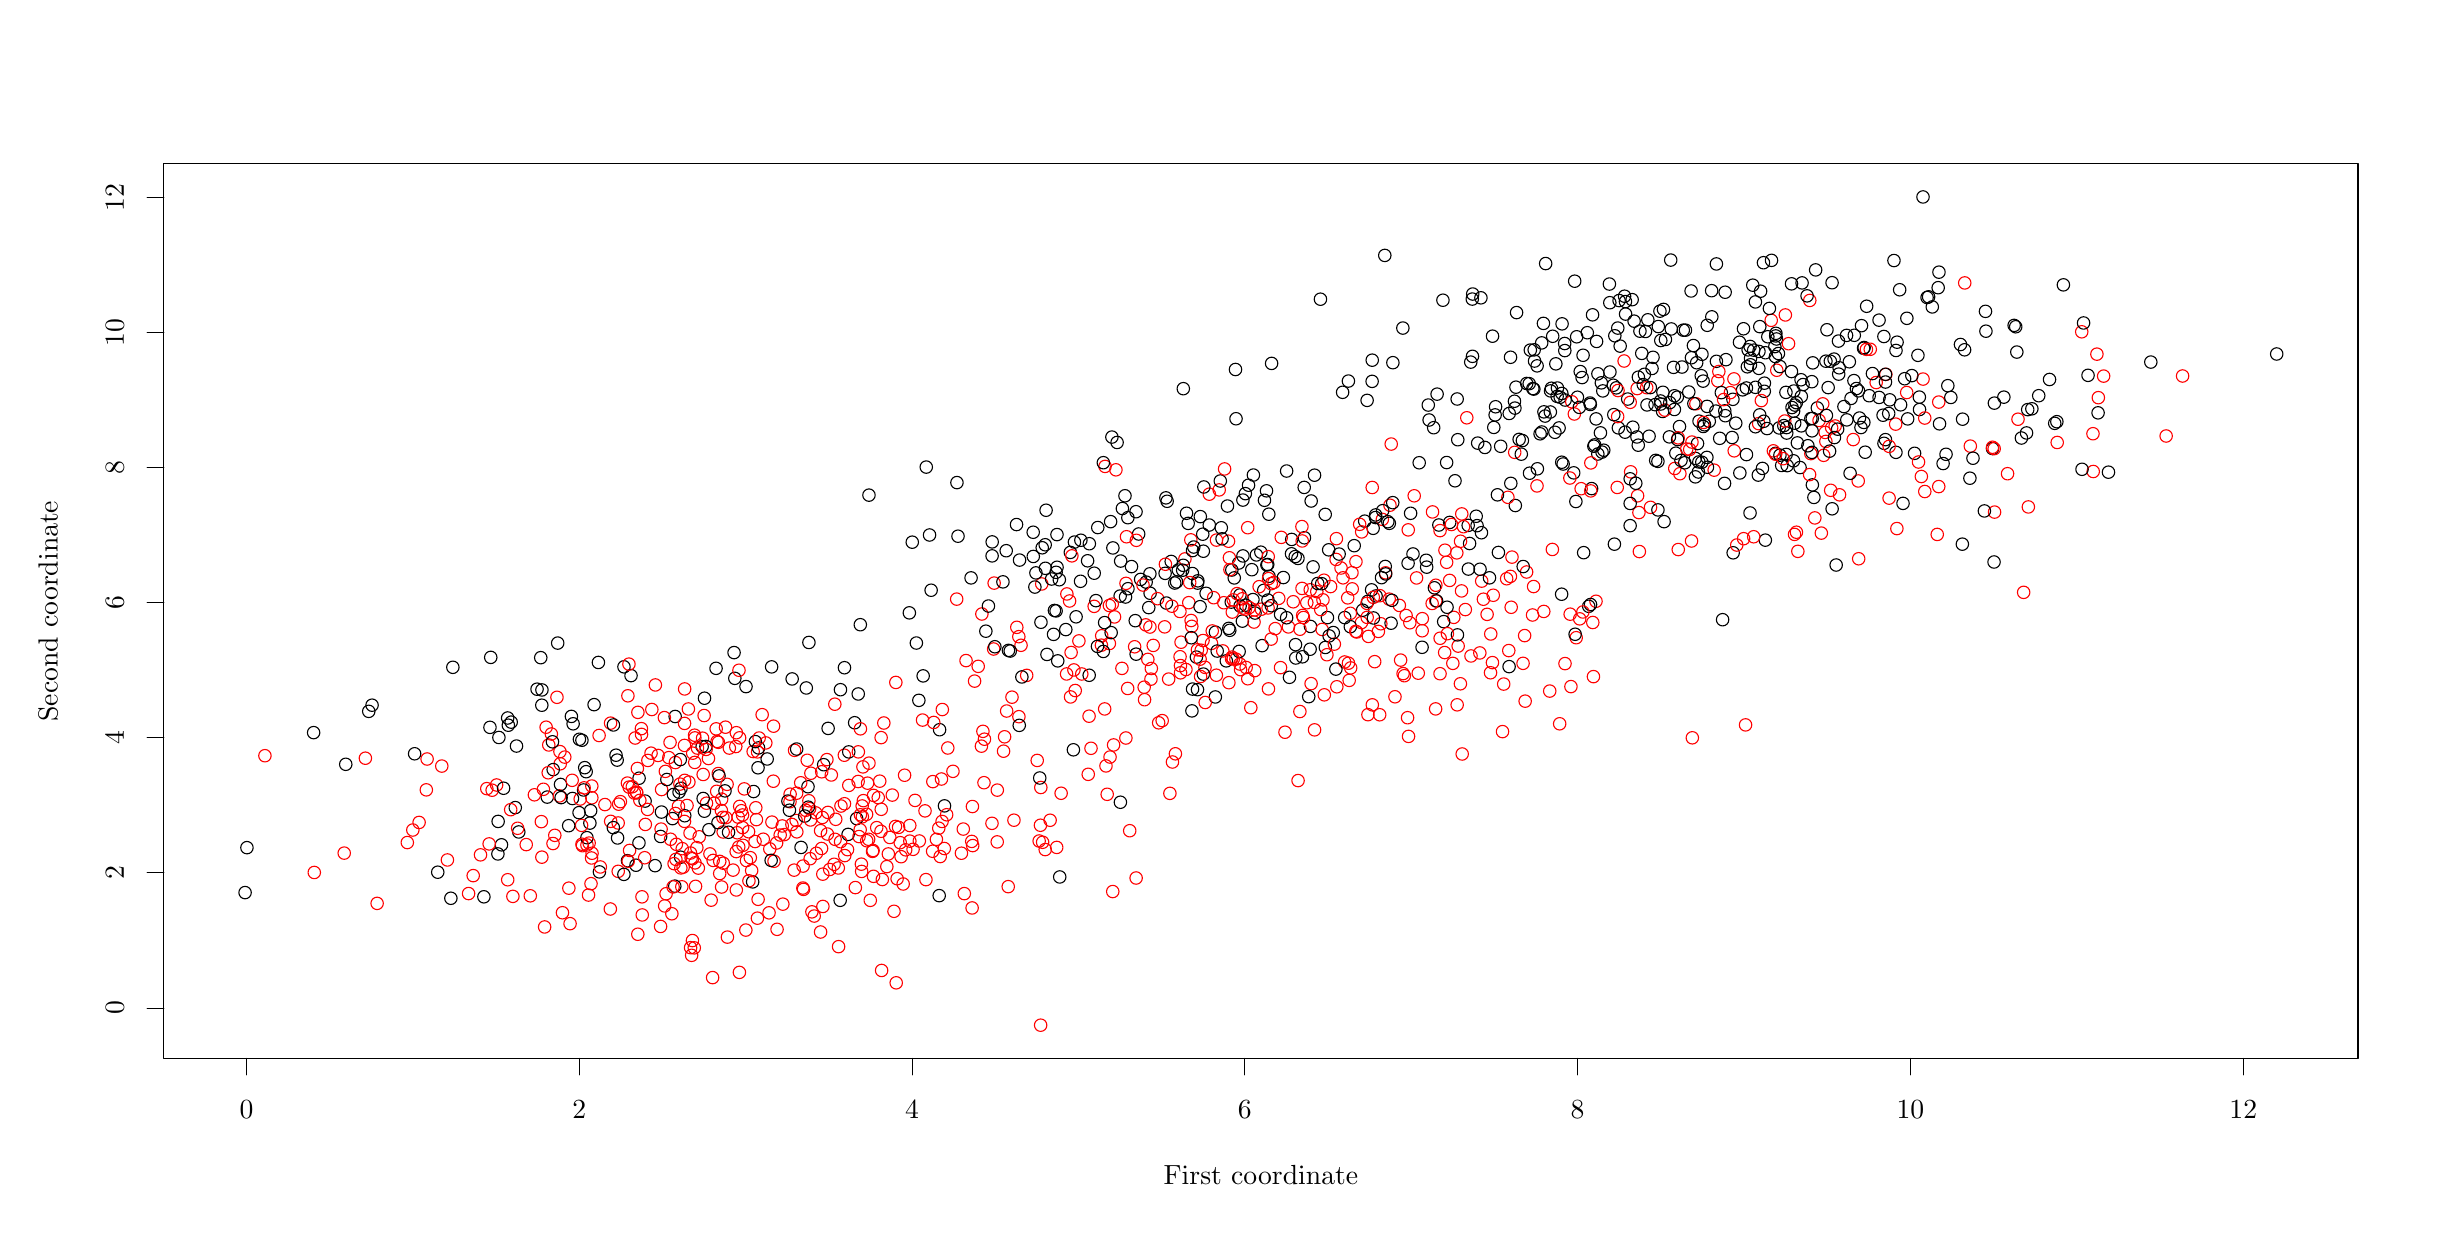
\begin{tikzpicture}[x=1pt,y=1pt]
\definecolor{fillColor}{RGB}{255,255,255}
\path[use as bounding box,fill=fillColor,fill opacity=0.00] (0,0) rectangle (867.24,433.62);
\begin{scope}
\path[clip] ( 49.20, 61.20) rectangle (842.04,384.42);
\definecolor{drawColor}{RGB}{0,0,0}

\path[draw=drawColor,line width= 0.4pt,line join=round,line cap=round] (438.93,219.17) circle (  2.25);
\definecolor{drawColor}{RGB}{255,0,0}

\path[draw=drawColor,line width= 0.4pt,line join=round,line cap=round] (536.35,242.31) circle (  2.25);

\path[draw=drawColor,line width= 0.4pt,line join=round,line cap=round] (329.22,144.36) circle (  2.25);
\definecolor{drawColor}{RGB}{0,0,0}

\path[draw=drawColor,line width= 0.4pt,line join=round,line cap=round] (255.53,198.50) circle (  2.25);
\definecolor{drawColor}{RGB}{255,0,0}

\path[draw=drawColor,line width= 0.4pt,line join=round,line cap=round] (383.53,184.82) circle (  2.25);
\definecolor{drawColor}{RGB}{0,0,0}

\path[draw=drawColor,line width= 0.4pt,line join=round,line cap=round] (463.53,217.26) circle (  2.25);
\definecolor{drawColor}{RGB}{255,0,0}

\path[draw=drawColor,line width= 0.4pt,line join=round,line cap=round] (392.09,121.46) circle (  2.25);
\definecolor{drawColor}{RGB}{0,0,0}

\path[draw=drawColor,line width= 0.4pt,line join=round,line cap=round] (686.89,336.35) circle (  2.25);

\path[draw=drawColor,line width= 0.4pt,line join=round,line cap=round] (233.96,184.71) circle (  2.25);
\definecolor{drawColor}{RGB}{255,0,0}

\path[draw=drawColor,line width= 0.4pt,line join=round,line cap=round] (746.29,286.89) circle (  2.25);
\definecolor{drawColor}{RGB}{0,0,0}

\path[draw=drawColor,line width= 0.4pt,line join=round,line cap=round] (417.58,303.16) circle (  2.25);

\path[draw=drawColor,line width= 0.4pt,line join=round,line cap=round] (197.09,182.07) circle (  2.25);

\path[draw=drawColor,line width= 0.4pt,line join=round,line cap=round] (601.91,318.75) circle (  2.25);

\path[draw=drawColor,line width= 0.4pt,line join=round,line cap=round] (581.51,285.72) circle (  2.25);

\path[draw=drawColor,line width= 0.4pt,line join=round,line cap=round] (434.91,226.05) circle (  2.25);
\definecolor{drawColor}{RGB}{255,0,0}

\path[draw=drawColor,line width= 0.4pt,line join=round,line cap=round] (249.58,175.39) circle (  2.25);
\definecolor{drawColor}{RGB}{0,0,0}

\path[draw=drawColor,line width= 0.4pt,line join=round,line cap=round] (215.47,202.66) circle (  2.25);

\path[draw=drawColor,line width= 0.4pt,line join=round,line cap=round] (590.89,301.86) circle (  2.25);
\definecolor{drawColor}{RGB}{255,0,0}

\path[draw=drawColor,line width= 0.4pt,line join=round,line cap=round] (167.83,158.08) circle (  2.25);

\path[draw=drawColor,line width= 0.4pt,line join=round,line cap=round] (460.48,230.99) circle (  2.25);

\path[draw=drawColor,line width= 0.4pt,line join=round,line cap=round] (275.50,156.63) circle (  2.25);
\definecolor{drawColor}{RGB}{0,0,0}

\path[draw=drawColor,line width= 0.4pt,line join=round,line cap=round] (169.92,135.05) circle (  2.25);

\path[draw=drawColor,line width= 0.4pt,line join=round,line cap=round] (213.01,168.96) circle (  2.25);

\path[draw=drawColor,line width= 0.4pt,line join=round,line cap=round] (456.76,248.69) circle (  2.25);

\path[draw=drawColor,line width= 0.4pt,line join=round,line cap=round] (535.93,268.95) circle (  2.25);

\path[draw=drawColor,line width= 0.4pt,line join=round,line cap=round] (235.37,157.39) circle (  2.25);

\path[draw=drawColor,line width= 0.4pt,line join=round,line cap=round] (368.32,207.14) circle (  2.25);

\path[draw=drawColor,line width= 0.4pt,line join=round,line cap=round] (577.35,334.65) circle (  2.25);

\path[draw=drawColor,line width= 0.4pt,line join=round,line cap=round] (458.13,210.67) circle (  2.25);

\path[draw=drawColor,line width= 0.4pt,line join=round,line cap=round] (206.23,204.24) circle (  2.25);

\path[draw=drawColor,line width= 0.4pt,line join=round,line cap=round] ( 79.23,137.32) circle (  2.25);
\definecolor{drawColor}{RGB}{255,0,0}

\path[draw=drawColor,line width= 0.4pt,line join=round,line cap=round] (235.16,152.27) circle (  2.25);
\definecolor{drawColor}{RGB}{0,0,0}

\path[draw=drawColor,line width= 0.4pt,line join=round,line cap=round] (620.01,324.81) circle (  2.25);
\definecolor{drawColor}{RGB}{255,0,0}

\path[draw=drawColor,line width= 0.4pt,line join=round,line cap=round] (632.04,309.83) circle (  2.25);
\definecolor{drawColor}{RGB}{0,0,0}

\path[draw=drawColor,line width= 0.4pt,line join=round,line cap=round] (461.35,249.29) circle (  2.25);

\path[draw=drawColor,line width= 0.4pt,line join=round,line cap=round] (646.08,346.09) circle (  2.25);
\definecolor{drawColor}{RGB}{255,0,0}

\path[draw=drawColor,line width= 0.4pt,line join=round,line cap=round] (189.23,178.39) circle (  2.25);

\path[draw=drawColor,line width= 0.4pt,line join=round,line cap=round] (203.86,155.34) circle (  2.25);

\path[draw=drawColor,line width= 0.4pt,line join=round,line cap=round] (516.41,243.83) circle (  2.25);
\definecolor{drawColor}{RGB}{0,0,0}

\path[draw=drawColor,line width= 0.4pt,line join=round,line cap=round] (442.75,226.96) circle (  2.25);
\definecolor{drawColor}{RGB}{255,0,0}

\path[draw=drawColor,line width= 0.4pt,line join=round,line cap=round] (314.70,144.64) circle (  2.25);

\path[draw=drawColor,line width= 0.4pt,line join=round,line cap=round] (581.74,264.46) circle (  2.25);

\path[draw=drawColor,line width= 0.4pt,line join=round,line cap=round] (241.34,123.34) circle (  2.25);

\path[draw=drawColor,line width= 0.4pt,line join=round,line cap=round] (719.20,292.13) circle (  2.25);

\path[draw=drawColor,line width= 0.4pt,line join=round,line cap=round] (535.79,235.34) circle (  2.25);
\definecolor{drawColor}{RGB}{0,0,0}

\path[draw=drawColor,line width= 0.4pt,line join=round,line cap=round] (632.91,288.98) circle (  2.25);

\path[draw=drawColor,line width= 0.4pt,line join=round,line cap=round] (579.77,335.33) circle (  2.25);

\path[draw=drawColor,line width= 0.4pt,line join=round,line cap=round] (226.71,130.81) circle (  2.25);

\path[draw=drawColor,line width= 0.4pt,line join=round,line cap=round] (644.35,292.36) circle (  2.25);
\definecolor{drawColor}{RGB}{255,0,0}

\path[draw=drawColor,line width= 0.4pt,line join=round,line cap=round] (412.29,198.23) circle (  2.25);
\definecolor{drawColor}{RGB}{0,0,0}

\path[draw=drawColor,line width= 0.4pt,line join=round,line cap=round] (469.67,220.45) circle (  2.25);
\definecolor{drawColor}{RGB}{255,0,0}

\path[draw=drawColor,line width= 0.4pt,line join=round,line cap=round] (684.88,306.64) circle (  2.25);

\path[draw=drawColor,line width= 0.4pt,line join=round,line cap=round] (248.05,153.36) circle (  2.25);
\definecolor{drawColor}{RGB}{0,0,0}

\path[draw=drawColor,line width= 0.4pt,line join=round,line cap=round] (544.50,313.15) circle (  2.25);

\path[draw=drawColor,line width= 0.4pt,line join=round,line cap=round] (487.23,228.27) circle (  2.25);
\definecolor{drawColor}{RGB}{255,0,0}

\path[draw=drawColor,line width= 0.4pt,line join=round,line cap=round] (512.02,207.82) circle (  2.25);
\definecolor{drawColor}{RGB}{0,0,0}

\path[draw=drawColor,line width= 0.4pt,line join=round,line cap=round] (460.64,206.28) circle (  2.25);

\path[draw=drawColor,line width= 0.4pt,line join=round,line cap=round] (394.95,240.88) circle (  2.25);

\path[draw=drawColor,line width= 0.4pt,line join=round,line cap=round] (448.48,257.81) circle (  2.25);

\path[draw=drawColor,line width= 0.4pt,line join=round,line cap=round] (235.94,133.87) circle (  2.25);
\definecolor{drawColor}{RGB}{255,0,0}

\path[draw=drawColor,line width= 0.4pt,line join=round,line cap=round] (358.18,184.64) circle (  2.25);
\definecolor{drawColor}{RGB}{0,0,0}

\path[draw=drawColor,line width= 0.4pt,line join=round,line cap=round] (438.05,228.63) circle (  2.25);
\definecolor{drawColor}{RGB}{255,0,0}

\path[draw=drawColor,line width= 0.4pt,line join=round,line cap=round] (240.87,101.11) circle (  2.25);
\definecolor{drawColor}{RGB}{0,0,0}

\path[draw=drawColor,line width= 0.4pt,line join=round,line cap=round] (566.22,282.86) circle (  2.25);
\definecolor{drawColor}{RGB}{255,0,0}

\path[draw=drawColor,line width= 0.4pt,line join=round,line cap=round] (467.74,216.16) circle (  2.25);
\definecolor{drawColor}{RGB}{0,0,0}

\path[draw=drawColor,line width= 0.4pt,line join=round,line cap=round] (654.56,310.72) circle (  2.25);

\path[draw=drawColor,line width= 0.4pt,line join=round,line cap=round] (484.00,298.94) circle (  2.25);

\path[draw=drawColor,line width= 0.4pt,line join=round,line cap=round] (589.08,276.90) circle (  2.25);
\definecolor{drawColor}{RGB}{255,0,0}

\path[draw=drawColor,line width= 0.4pt,line join=round,line cap=round] (186.80,108.66) circle (  2.25);

\path[draw=drawColor,line width= 0.4pt,line join=round,line cap=round] (649.77,284.11) circle (  2.25);

\path[draw=drawColor,line width= 0.4pt,line join=round,line cap=round] (316.36,124.19) circle (  2.25);

\path[draw=drawColor,line width= 0.4pt,line join=round,line cap=round] (293.02,101.55) circle (  2.25);
\definecolor{drawColor}{RGB}{0,0,0}

\path[draw=drawColor,line width= 0.4pt,line join=round,line cap=round] (561.68,307.18) circle (  2.25);

\path[draw=drawColor,line width= 0.4pt,line join=round,line cap=round] (203.43,150.67) circle (  2.25);

\path[draw=drawColor,line width= 0.4pt,line join=round,line cap=round] (261.97,124.95) circle (  2.25);

\path[draw=drawColor,line width= 0.4pt,line join=round,line cap=round] (679.33,292.25) circle (  2.25);
\definecolor{drawColor}{RGB}{255,0,0}

\path[draw=drawColor,line width= 0.4pt,line join=round,line cap=round] (665.81,317.40) circle (  2.25);

\path[draw=drawColor,line width= 0.4pt,line join=round,line cap=round] (280.18,130.67) circle (  2.25);

\path[draw=drawColor,line width= 0.4pt,line join=round,line cap=round] (250.07,127.96) circle (  2.25);
\definecolor{drawColor}{RGB}{0,0,0}

\path[draw=drawColor,line width= 0.4pt,line join=round,line cap=round] (577.21,287.45) circle (  2.25);

\path[draw=drawColor,line width= 0.4pt,line join=round,line cap=round] (508.33,231.21) circle (  2.25);
\definecolor{drawColor}{RGB}{255,0,0}

\path[draw=drawColor,line width= 0.4pt,line join=round,line cap=round] (214.17,153.94) circle (  2.25);
\definecolor{drawColor}{RGB}{0,0,0}

\path[draw=drawColor,line width= 0.4pt,line join=round,line cap=round] (637.34,309.36) circle (  2.25);

\path[draw=drawColor,line width= 0.4pt,line join=round,line cap=round] (603.72,273.06) circle (  2.25);

\path[draw=drawColor,line width= 0.4pt,line join=round,line cap=round] (485.62,230.47) circle (  2.25);
\definecolor{drawColor}{RGB}{255,0,0}

\path[draw=drawColor,line width= 0.4pt,line join=round,line cap=round] (685.52,266.01) circle (  2.25);

\path[draw=drawColor,line width= 0.4pt,line join=round,line cap=round] (430.55,266.59) circle (  2.25);

\path[draw=drawColor,line width= 0.4pt,line join=round,line cap=round] (508.81,226.53) circle (  2.25);
\definecolor{drawColor}{RGB}{0,0,0}

\path[draw=drawColor,line width= 0.4pt,line join=round,line cap=round] (554.33,276.59) circle (  2.25);

\path[draw=drawColor,line width= 0.4pt,line join=round,line cap=round] (610.02,295.07) circle (  2.25);
\definecolor{drawColor}{RGB}{255,0,0}

\path[draw=drawColor,line width= 0.4pt,line join=round,line cap=round] (261.12,133.70) circle (  2.25);
\definecolor{drawColor}{RGB}{0,0,0}

\path[draw=drawColor,line width= 0.4pt,line join=round,line cap=round] (304.00,264.70) circle (  2.25);

\path[draw=drawColor,line width= 0.4pt,line join=round,line cap=round] (617.21,290.70) circle (  2.25);

\path[draw=drawColor,line width= 0.4pt,line join=round,line cap=round] (437.62,240.16) circle (  2.25);
\definecolor{drawColor}{RGB}{255,0,0}

\path[draw=drawColor,line width= 0.4pt,line join=round,line cap=round] (281.17,150.82) circle (  2.25);

\path[draw=drawColor,line width= 0.4pt,line join=round,line cap=round] (494.07,191.84) circle (  2.25);

\path[draw=drawColor,line width= 0.4pt,line join=round,line cap=round] (625.48,290.54) circle (  2.25);

\path[draw=drawColor,line width= 0.4pt,line join=round,line cap=round] (308.34,143.24) circle (  2.25);
\definecolor{drawColor}{RGB}{0,0,0}

\path[draw=drawColor,line width= 0.4pt,line join=round,line cap=round] (554.29,228.90) circle (  2.25);

\path[draw=drawColor,line width= 0.4pt,line join=round,line cap=round] (461.27,267.49) circle (  2.25);
\definecolor{drawColor}{RGB}{255,0,0}

\path[draw=drawColor,line width= 0.4pt,line join=round,line cap=round] (651.51,266.45) circle (  2.25);

\path[draw=drawColor,line width= 0.4pt,line join=round,line cap=round] (190.48,141.77) circle (  2.25);

\path[draw=drawColor,line width= 0.4pt,line join=round,line cap=round] (263.69,111.84) circle (  2.25);

\path[draw=drawColor,line width= 0.4pt,line join=round,line cap=round] (472.80,241.47) circle (  2.25);

\path[draw=drawColor,line width= 0.4pt,line join=round,line cap=round] (252.85,104.99) circle (  2.25);

\path[draw=drawColor,line width= 0.4pt,line join=round,line cap=round] (481.96,218.63) circle (  2.25);
\definecolor{drawColor}{RGB}{0,0,0}

\path[draw=drawColor,line width= 0.4pt,line join=round,line cap=round] (558.66,272.75) circle (  2.25);

\path[draw=drawColor,line width= 0.4pt,line join=round,line cap=round] (569.51,280.93) circle (  2.25);

\path[draw=drawColor,line width= 0.4pt,line join=round,line cap=round] (675.11,316.97) circle (  2.25);
\definecolor{drawColor}{RGB}{255,0,0}

\path[draw=drawColor,line width= 0.4pt,line join=round,line cap=round] (323.36,183.42) circle (  2.25);
\definecolor{drawColor}{RGB}{0,0,0}

\path[draw=drawColor,line width= 0.4pt,line join=round,line cap=round] (660.80,303.22) circle (  2.25);

\path[draw=drawColor,line width= 0.4pt,line join=round,line cap=round] (658.25,312.89) circle (  2.25);

\path[draw=drawColor,line width= 0.4pt,line join=round,line cap=round] (331.29,152.41) circle (  2.25);

\path[draw=drawColor,line width= 0.4pt,line join=round,line cap=round] (502.82,276.40) circle (  2.25);

\path[draw=drawColor,line width= 0.4pt,line join=round,line cap=round] (103.33,178.88) circle (  2.25);
\definecolor{drawColor}{RGB}{255,0,0}

\path[draw=drawColor,line width= 0.4pt,line join=round,line cap=round] (263.73,171.92) circle (  2.25);

\path[draw=drawColor,line width= 0.4pt,line join=round,line cap=round] (225.54,187.24) circle (  2.25);

\path[draw=drawColor,line width= 0.4pt,line join=round,line cap=round] (244.09,163.76) circle (  2.25);
\definecolor{drawColor}{RGB}{0,0,0}

\path[draw=drawColor,line width= 0.4pt,line join=round,line cap=round] (505.35,241.16) circle (  2.25);
\definecolor{drawColor}{RGB}{255,0,0}

\path[draw=drawColor,line width= 0.4pt,line join=round,line cap=round] (566.71,226.35) circle (  2.25);

\path[draw=drawColor,line width= 0.4pt,line join=round,line cap=round] (306.80,144.55) circle (  2.25);
\definecolor{drawColor}{RGB}{0,0,0}

\path[draw=drawColor,line width= 0.4pt,line join=round,line cap=round] (380.57,248.40) circle (  2.25);
\definecolor{drawColor}{RGB}{255,0,0}

\path[draw=drawColor,line width= 0.4pt,line join=round,line cap=round] (159.32,120.73) circle (  2.25);

\path[draw=drawColor,line width= 0.4pt,line join=round,line cap=round] (400.00,209.90) circle (  2.25);
\definecolor{drawColor}{RGB}{0,0,0}

\path[draw=drawColor,line width= 0.4pt,line join=round,line cap=round] (164.86,119.56) circle (  2.25);
\definecolor{drawColor}{RGB}{255,0,0}

\path[draw=drawColor,line width= 0.4pt,line join=round,line cap=round] (510.35,200.17) circle (  2.25);

\path[draw=drawColor,line width= 0.4pt,line join=round,line cap=round] (426.98,265.05) circle (  2.25);
\definecolor{drawColor}{RGB}{0,0,0}

\path[draw=drawColor,line width= 0.4pt,line join=round,line cap=round] (268.82,202.64) circle (  2.25);
\definecolor{drawColor}{RGB}{255,0,0}

\path[draw=drawColor,line width= 0.4pt,line join=round,line cap=round] (241.13,131.82) circle (  2.25);

\path[draw=drawColor,line width= 0.4pt,line join=round,line cap=round] (353.75,186.69) circle (  2.25);
\definecolor{drawColor}{RGB}{0,0,0}

\path[draw=drawColor,line width= 0.4pt,line join=round,line cap=round] (735.60,340.68) circle (  2.25);
\definecolor{drawColor}{RGB}{255,0,0}

\path[draw=drawColor,line width= 0.4pt,line join=round,line cap=round] (392.73,220.69) circle (  2.25);
\definecolor{drawColor}{RGB}{0,0,0}

\path[draw=drawColor,line width= 0.4pt,line join=round,line cap=round] (683.61,295.63) circle (  2.25);

\path[draw=drawColor,line width= 0.4pt,line join=round,line cap=round] (493.31,312.56) circle (  2.25);

\path[draw=drawColor,line width= 0.4pt,line join=round,line cap=round] (152.92,119.03) circle (  2.25);
\definecolor{drawColor}{RGB}{255,0,0}

\path[draw=drawColor,line width= 0.4pt,line join=round,line cap=round] (557.37,221.69) circle (  2.25);

\path[draw=drawColor,line width= 0.4pt,line join=round,line cap=round] (239.73,133.58) circle (  2.25);

\path[draw=drawColor,line width= 0.4pt,line join=round,line cap=round] (305.65,156.21) circle (  2.25);
\definecolor{drawColor}{RGB}{0,0,0}

\path[draw=drawColor,line width= 0.4pt,line join=round,line cap=round] (748.13,294.44) circle (  2.25);
\definecolor{drawColor}{RGB}{255,0,0}

\path[draw=drawColor,line width= 0.4pt,line join=round,line cap=round] (579.23,273.12) circle (  2.25);
\definecolor{drawColor}{RGB}{0,0,0}

\path[draw=drawColor,line width= 0.4pt,line join=round,line cap=round] (148.18,128.45) circle (  2.25);
\definecolor{drawColor}{RGB}{255,0,0}

\path[draw=drawColor,line width= 0.4pt,line join=round,line cap=round] (403.44,195.30) circle (  2.25);
\definecolor{drawColor}{RGB}{0,0,0}

\path[draw=drawColor,line width= 0.4pt,line join=round,line cap=round] (565.46,329.85) circle (  2.25);
\definecolor{drawColor}{RGB}{255,0,0}

\path[draw=drawColor,line width= 0.4pt,line join=round,line cap=round] (648.98,279.09) circle (  2.25);
\definecolor{drawColor}{RGB}{0,0,0}

\path[draw=drawColor,line width= 0.4pt,line join=round,line cap=round] (710.54,240.54) circle (  2.25);
\definecolor{drawColor}{RGB}{255,0,0}

\path[draw=drawColor,line width= 0.4pt,line join=round,line cap=round] (338.08,144.04) circle (  2.25);

\path[draw=drawColor,line width= 0.4pt,line join=round,line cap=round] (661.63,241.71) circle (  2.25);
\definecolor{drawColor}{RGB}{0,0,0}

\path[draw=drawColor,line width= 0.4pt,line join=round,line cap=round] (398.87,238.88) circle (  2.25);
\definecolor{drawColor}{RGB}{255,0,0}

\path[draw=drawColor,line width= 0.4pt,line join=round,line cap=round] (366.43,232.60) circle (  2.25);

\path[draw=drawColor,line width= 0.4pt,line join=round,line cap=round] (379.86,212.02) circle (  2.25);

\path[draw=drawColor,line width= 0.4pt,line join=round,line cap=round] (459.73,216.24) circle (  2.25);
\definecolor{drawColor}{RGB}{0,0,0}

\path[draw=drawColor,line width= 0.4pt,line join=round,line cap=round] (699.17,292.15) circle (  2.25);

\path[draw=drawColor,line width= 0.4pt,line join=round,line cap=round] (547.12,287.51) circle (  2.25);
\definecolor{drawColor}{RGB}{255,0,0}

\path[draw=drawColor,line width= 0.4pt,line join=round,line cap=round] (516.90,210.15) circle (  2.25);
\definecolor{drawColor}{RGB}{0,0,0}

\path[draw=drawColor,line width= 0.4pt,line join=round,line cap=round] (376.76,244.01) circle (  2.25);
\definecolor{drawColor}{RGB}{255,0,0}

\path[draw=drawColor,line width= 0.4pt,line join=round,line cap=round] (437.00,229.12) circle (  2.25);
\definecolor{drawColor}{RGB}{0,0,0}

\path[draw=drawColor,line width= 0.4pt,line join=round,line cap=round] (380.45,233.57) circle (  2.25);
\definecolor{drawColor}{RGB}{255,0,0}

\path[draw=drawColor,line width= 0.4pt,line join=round,line cap=round] (319.93,136.72) circle (  2.25);
\definecolor{drawColor}{RGB}{0,0,0}

\path[draw=drawColor,line width= 0.4pt,line join=round,line cap=round] (603.09,312.54) circle (  2.25);

\path[draw=drawColor,line width= 0.4pt,line join=round,line cap=round] (622.38,318.43) circle (  2.25);

\path[draw=drawColor,line width= 0.4pt,line join=round,line cap=round] (564.66,297.46) circle (  2.25);

\path[draw=drawColor,line width= 0.4pt,line join=round,line cap=round] (293.59,118.29) circle (  2.25);
\definecolor{drawColor}{RGB}{255,0,0}

\path[draw=drawColor,line width= 0.4pt,line join=round,line cap=round] (582.22,258.40) circle (  2.25);
\definecolor{drawColor}{RGB}{0,0,0}

\path[draw=drawColor,line width= 0.4pt,line join=round,line cap=round] (279.46,137.40) circle (  2.25);
\definecolor{drawColor}{RGB}{255,0,0}

\path[draw=drawColor,line width= 0.4pt,line join=round,line cap=round] (630.02,327.87) circle (  2.25);
\definecolor{drawColor}{RGB}{0,0,0}

\path[draw=drawColor,line width= 0.4pt,line join=round,line cap=round] (718.37,325.54) circle (  2.25);
\definecolor{drawColor}{RGB}{255,0,0}

\path[draw=drawColor,line width= 0.4pt,line join=round,line cap=round] (484.47,213.65) circle (  2.25);
\definecolor{drawColor}{RGB}{0,0,0}

\path[draw=drawColor,line width= 0.4pt,line join=round,line cap=round] (463.41,209.02) circle (  2.25);
\definecolor{drawColor}{RGB}{255,0,0}

\path[draw=drawColor,line width= 0.4pt,line join=round,line cap=round] (690.56,298.33) circle (  2.25);
\definecolor{drawColor}{RGB}{0,0,0}

\path[draw=drawColor,line width= 0.4pt,line join=round,line cap=round] (185.40,205.97) circle (  2.25);

\path[draw=drawColor,line width= 0.4pt,line join=round,line cap=round] (335.79,269.23) circle (  2.25);

\path[draw=drawColor,line width= 0.4pt,line join=round,line cap=round] (554.45,326.59) circle (  2.25);
\definecolor{drawColor}{RGB}{255,0,0}

\path[draw=drawColor,line width= 0.4pt,line join=round,line cap=round] (602.80,297.71) circle (  2.25);

\path[draw=drawColor,line width= 0.4pt,line join=round,line cap=round] (647.31,291.68) circle (  2.25);

\path[draw=drawColor,line width= 0.4pt,line join=round,line cap=round] (448.22,223.94) circle (  2.25);
\definecolor{drawColor}{RGB}{0,0,0}

\path[draw=drawColor,line width= 0.4pt,line join=round,line cap=round] (717.80,326.03) circle (  2.25);
\definecolor{drawColor}{RGB}{255,0,0}

\path[draw=drawColor,line width= 0.4pt,line join=round,line cap=round] (318.77,139.68) circle (  2.25);

\path[draw=drawColor,line width= 0.4pt,line join=round,line cap=round] (690.56,267.79) circle (  2.25);

\path[draw=drawColor,line width= 0.4pt,line join=round,line cap=round] (188.29,174.43) circle (  2.25);

\path[draw=drawColor,line width= 0.4pt,line join=round,line cap=round] (418.17,241.64) circle (  2.25);
\definecolor{drawColor}{RGB}{0,0,0}

\path[draw=drawColor,line width= 0.4pt,line join=round,line cap=round] (554.36,301.44) circle (  2.25);
\definecolor{drawColor}{RGB}{255,0,0}

\path[draw=drawColor,line width= 0.4pt,line join=round,line cap=round] (291.40,131.31) circle (  2.25);

\path[draw=drawColor,line width= 0.4pt,line join=round,line cap=round] (253.54,173.31) circle (  2.25);
\definecolor{drawColor}{RGB}{0,0,0}

\path[draw=drawColor,line width= 0.4pt,line join=round,line cap=round] (438.11,224.63) circle (  2.25);
\definecolor{drawColor}{RGB}{255,0,0}

\path[draw=drawColor,line width= 0.4pt,line join=round,line cap=round] (349.23,232.92) circle (  2.25);

\path[draw=drawColor,line width= 0.4pt,line join=round,line cap=round] (265.40,185.37) circle (  2.25);

\path[draw=drawColor,line width= 0.4pt,line join=round,line cap=round] (485.88,188.92) circle (  2.25);
\definecolor{drawColor}{RGB}{0,0,0}

\path[draw=drawColor,line width= 0.4pt,line join=round,line cap=round] (640.89,289.73) circle (  2.25);
\definecolor{drawColor}{RGB}{255,0,0}

\path[draw=drawColor,line width= 0.4pt,line join=round,line cap=round] (648.13,250.98) circle (  2.25);
\definecolor{drawColor}{RGB}{0,0,0}

\path[draw=drawColor,line width= 0.4pt,line join=round,line cap=round] (318.59,222.16) circle (  2.25);

\path[draw=drawColor,line width= 0.4pt,line join=round,line cap=round] (566.74,292.25) circle (  2.25);

\path[draw=drawColor,line width= 0.4pt,line join=round,line cap=round] (123.25,186.57) circle (  2.25);
\definecolor{drawColor}{RGB}{255,0,0}

\path[draw=drawColor,line width= 0.4pt,line join=round,line cap=round] (464.94,225.94) circle (  2.25);
\definecolor{drawColor}{RGB}{0,0,0}

\path[draw=drawColor,line width= 0.4pt,line join=round,line cap=round] (363.95,231.49) circle (  2.25);
\definecolor{drawColor}{RGB}{255,0,0}

\path[draw=drawColor,line width= 0.4pt,line join=round,line cap=round] (565.55,218.68) circle (  2.25);
\definecolor{drawColor}{RGB}{0,0,0}

\path[draw=drawColor,line width= 0.4pt,line join=round,line cap=round] (420.70,186.74) circle (  2.25);

\path[draw=drawColor,line width= 0.4pt,line join=round,line cap=round] (293.70,194.39) circle (  2.25);

\path[draw=drawColor,line width= 0.4pt,line join=round,line cap=round] (530.26,293.69) circle (  2.25);
\definecolor{drawColor}{RGB}{255,0,0}

\path[draw=drawColor,line width= 0.4pt,line join=round,line cap=round] (529.58,228.52) circle (  2.25);
\definecolor{drawColor}{RGB}{0,0,0}

\path[draw=drawColor,line width= 0.4pt,line join=round,line cap=round] (564.08,224.53) circle (  2.25);

\path[draw=drawColor,line width= 0.4pt,line join=round,line cap=round] (596.88,289.48) circle (  2.25);
\definecolor{drawColor}{RGB}{255,0,0}

\path[draw=drawColor,line width= 0.4pt,line join=round,line cap=round] (486.24,227.78) circle (  2.25);
\definecolor{drawColor}{RGB}{0,0,0}

\path[draw=drawColor,line width= 0.4pt,line join=round,line cap=round] (503.86,209.72) circle (  2.25);

\path[draw=drawColor,line width= 0.4pt,line join=round,line cap=round] (670.77,283.43) circle (  2.25);

\path[draw=drawColor,line width= 0.4pt,line join=round,line cap=round] (296.46,142.11) circle (  2.25);

\path[draw=drawColor,line width= 0.4pt,line join=round,line cap=round] (605.47,289.51) circle (  2.25);

\path[draw=drawColor,line width= 0.4pt,line join=round,line cap=round] (436.63,292.30) circle (  2.25);

\path[draw=drawColor,line width= 0.4pt,line join=round,line cap=round] (590.78,294.94) circle (  2.25);

\path[draw=drawColor,line width= 0.4pt,line join=round,line cap=round] (367.68,246.77) circle (  2.25);
\definecolor{drawColor}{RGB}{255,0,0}

\path[draw=drawColor,line width= 0.4pt,line join=round,line cap=round] (365.96,145.42) circle (  2.25);
\definecolor{drawColor}{RGB}{0,0,0}

\path[draw=drawColor,line width= 0.4pt,line join=round,line cap=round] (543.88,303.20) circle (  2.25);

\path[draw=drawColor,line width= 0.4pt,line join=round,line cap=round] (559.01,342.01) circle (  2.25);

\path[draw=drawColor,line width= 0.4pt,line join=round,line cap=round] (346.24,215.54) circle (  2.25);

\path[draw=drawColor,line width= 0.4pt,line join=round,line cap=round] (597.77,310.99) circle (  2.25);
\definecolor{drawColor}{RGB}{255,0,0}

\path[draw=drawColor,line width= 0.4pt,line join=round,line cap=round] (315.29,139.12) circle (  2.25);

\path[draw=drawColor,line width= 0.4pt,line join=round,line cap=round] (390.87,211.08) circle (  2.25);

\path[draw=drawColor,line width= 0.4pt,line join=round,line cap=round] (525.41,233.63) circle (  2.25);

\path[draw=drawColor,line width= 0.4pt,line join=round,line cap=round] (463.45,230.50) circle (  2.25);

\path[draw=drawColor,line width= 0.4pt,line join=round,line cap=round] (486.74,204.52) circle (  2.25);
\definecolor{drawColor}{RGB}{0,0,0}

\path[draw=drawColor,line width= 0.4pt,line join=round,line cap=round] (357.32,254.07) circle (  2.25);

\path[draw=drawColor,line width= 0.4pt,line join=round,line cap=round] (468.91,209.66) circle (  2.25);

\path[draw=drawColor,line width= 0.4pt,line join=round,line cap=round] (606.84,296.77) circle (  2.25);

\path[draw=drawColor,line width= 0.4pt,line join=round,line cap=round] (177.46,142.99) circle (  2.25);
\definecolor{drawColor}{RGB}{255,0,0}

\path[draw=drawColor,line width= 0.4pt,line join=round,line cap=round] (288.80,169.13) circle (  2.25);

\path[draw=drawColor,line width= 0.4pt,line join=round,line cap=round] (489.51,255.94) circle (  2.25);

\path[draw=drawColor,line width= 0.4pt,line join=round,line cap=round] (435.28,222.44) circle (  2.25);

\path[draw=drawColor,line width= 0.4pt,line join=round,line cap=round] (524.73,207.68) circle (  2.25);
\definecolor{drawColor}{RGB}{0,0,0}

\path[draw=drawColor,line width= 0.4pt,line join=round,line cap=round] (663.59,318.04) circle (  2.25);
\definecolor{drawColor}{RGB}{255,0,0}

\path[draw=drawColor,line width= 0.4pt,line join=round,line cap=round] (272.88,116.91) circle (  2.25);
\definecolor{drawColor}{RGB}{0,0,0}

\path[draw=drawColor,line width= 0.4pt,line join=round,line cap=round] (223.10,154.15) circle (  2.25);

\path[draw=drawColor,line width= 0.4pt,line join=round,line cap=round] (594.72,310.87) circle (  2.25);
\definecolor{drawColor}{RGB}{255,0,0}

\path[draw=drawColor,line width= 0.4pt,line join=round,line cap=round] (245.29,153.38) circle (  2.25);
\definecolor{drawColor}{RGB}{0,0,0}

\path[draw=drawColor,line width= 0.4pt,line join=round,line cap=round] (405.10,224.06) circle (  2.25);
\definecolor{drawColor}{RGB}{255,0,0}

\path[draw=drawColor,line width= 0.4pt,line join=round,line cap=round] (200.46,138.03) circle (  2.25);

\path[draw=drawColor,line width= 0.4pt,line join=round,line cap=round] (659.66,284.78) circle (  2.25);
\definecolor{drawColor}{RGB}{0,0,0}

\path[draw=drawColor,line width= 0.4pt,line join=round,line cap=round] (565.94,282.37) circle (  2.25);
\definecolor{drawColor}{RGB}{255,0,0}

\path[draw=drawColor,line width= 0.4pt,line join=round,line cap=round] (645.78,256.47) circle (  2.25);
\definecolor{drawColor}{RGB}{0,0,0}

\path[draw=drawColor,line width= 0.4pt,line join=round,line cap=round] (298.83,182.45) circle (  2.25);
\definecolor{drawColor}{RGB}{255,0,0}

\path[draw=drawColor,line width= 0.4pt,line join=round,line cap=round] (543.78,221.39) circle (  2.25);

\path[draw=drawColor,line width= 0.4pt,line join=round,line cap=round] (534.42,234.49) circle (  2.25);
\definecolor{drawColor}{RGB}{0,0,0}

\path[draw=drawColor,line width= 0.4pt,line join=round,line cap=round] (196.86,155.08) circle (  2.25);
\definecolor{drawColor}{RGB}{255,0,0}

\path[draw=drawColor,line width= 0.4pt,line join=round,line cap=round] (269.44,161.33) circle (  2.25);

\path[draw=drawColor,line width= 0.4pt,line join=round,line cap=round] (375.41,200.08) circle (  2.25);
\definecolor{drawColor}{RGB}{0,0,0}

\path[draw=drawColor,line width= 0.4pt,line join=round,line cap=round] (586.95,310.47) circle (  2.25);
\definecolor{drawColor}{RGB}{255,0,0}

\path[draw=drawColor,line width= 0.4pt,line join=round,line cap=round] (322.19,139.73) circle (  2.25);

\path[draw=drawColor,line width= 0.4pt,line join=round,line cap=round] (239.54,101.18) circle (  2.25);
\definecolor{drawColor}{RGB}{0,0,0}

\path[draw=drawColor,line width= 0.4pt,line join=round,line cap=round] (470.27,213.83) circle (  2.25);

\path[draw=drawColor,line width= 0.4pt,line join=round,line cap=round] (693.84,304.25) circle (  2.25);
\definecolor{drawColor}{RGB}{255,0,0}

\path[draw=drawColor,line width= 0.4pt,line join=round,line cap=round] (488.55,185.34) circle (  2.25);
\definecolor{drawColor}{RGB}{0,0,0}

\path[draw=drawColor,line width= 0.4pt,line join=round,line cap=round] (372.21,204.81) circle (  2.25);

\path[draw=drawColor,line width= 0.4pt,line join=round,line cap=round] (545.53,274.21) circle (  2.25);

\path[draw=drawColor,line width= 0.4pt,line join=round,line cap=round] (578.17,299.42) circle (  2.25);
\definecolor{drawColor}{RGB}{255,0,0}

\path[draw=drawColor,line width= 0.4pt,line join=round,line cap=round] (389.64,166.85) circle (  2.25);

\path[draw=drawColor,line width= 0.4pt,line join=round,line cap=round] (378.53,194.10) circle (  2.25);

\path[draw=drawColor,line width= 0.4pt,line join=round,line cap=round] (210.66,146.83) circle (  2.25);
\definecolor{drawColor}{RGB}{0,0,0}

\path[draw=drawColor,line width= 0.4pt,line join=round,line cap=round] (422.32,206.18) circle (  2.25);

\path[draw=drawColor,line width= 0.4pt,line join=round,line cap=round] (446.91,262.84) circle (  2.25);

\path[draw=drawColor,line width= 0.4pt,line join=round,line cap=round] (417.36,237.58) circle (  2.25);

\path[draw=drawColor,line width= 0.4pt,line join=round,line cap=round] (153.64,202.49) circle (  2.25);
\definecolor{drawColor}{RGB}{255,0,0}

\path[draw=drawColor,line width= 0.4pt,line join=round,line cap=round] (241.80,137.32) circle (  2.25);

\path[draw=drawColor,line width= 0.4pt,line join=round,line cap=round] (236.37,123.17) circle (  2.25);
\definecolor{drawColor}{RGB}{0,0,0}

\path[draw=drawColor,line width= 0.4pt,line join=round,line cap=round] (496.92,325.07) circle (  2.25);

\path[draw=drawColor,line width= 0.4pt,line join=round,line cap=round] (591.10,331.81) circle (  2.25);
\definecolor{drawColor}{RGB}{255,0,0}

\path[draw=drawColor,line width= 0.4pt,line join=round,line cap=round] (490.66,236.62) circle (  2.25);
\definecolor{drawColor}{RGB}{0,0,0}

\path[draw=drawColor,line width= 0.4pt,line join=round,line cap=round] (581.98,282.75) circle (  2.25);
\definecolor{drawColor}{RGB}{255,0,0}

\path[draw=drawColor,line width= 0.4pt,line join=round,line cap=round] (502.48,200.36) circle (  2.25);
\definecolor{drawColor}{RGB}{0,0,0}

\path[draw=drawColor,line width= 0.4pt,line join=round,line cap=round] (203.16,146.19) circle (  2.25);

\path[draw=drawColor,line width= 0.4pt,line join=round,line cap=round] (590.12,320.58) circle (  2.25);
\definecolor{drawColor}{RGB}{255,0,0}

\path[draw=drawColor,line width= 0.4pt,line join=round,line cap=round] (685.50,292.56) circle (  2.25);
\definecolor{drawColor}{RGB}{0,0,0}

\path[draw=drawColor,line width= 0.4pt,line join=round,line cap=round] (433.12,204.81) circle (  2.25);

\path[draw=drawColor,line width= 0.4pt,line join=round,line cap=round] (490.71,236.22) circle (  2.25);
\definecolor{drawColor}{RGB}{255,0,0}

\path[draw=drawColor,line width= 0.4pt,line join=round,line cap=round] (478.62,230.83) circle (  2.25);

\path[draw=drawColor,line width= 0.4pt,line join=round,line cap=round] (352.63,172.18) circle (  2.25);

\path[draw=drawColor,line width= 0.4pt,line join=round,line cap=round] (259.73,132.66) circle (  2.25);

\path[draw=drawColor,line width= 0.4pt,line join=round,line cap=round] (431.86,208.40) circle (  2.25);
\definecolor{drawColor}{RGB}{0,0,0}

\path[draw=drawColor,line width= 0.4pt,line join=round,line cap=round] (654.33,320.37) circle (  2.25);
\definecolor{drawColor}{RGB}{255,0,0}

\path[draw=drawColor,line width= 0.4pt,line join=round,line cap=round] (535.19,208.53) circle (  2.25);
\definecolor{drawColor}{RGB}{0,0,0}

\path[draw=drawColor,line width= 0.4pt,line join=round,line cap=round] (483.13,255.30) circle (  2.25);

\path[draw=drawColor,line width= 0.4pt,line join=round,line cap=round] (631.57,279.80) circle (  2.25);
\definecolor{drawColor}{RGB}{255,0,0}

\path[draw=drawColor,line width= 0.4pt,line join=round,line cap=round] (338.45,120.71) circle (  2.25);
\definecolor{drawColor}{RGB}{0,0,0}

\path[draw=drawColor,line width= 0.4pt,line join=round,line cap=round] (638.08,277.09) circle (  2.25);
\definecolor{drawColor}{RGB}{255,0,0}

\path[draw=drawColor,line width= 0.4pt,line join=round,line cap=round] (203.93,135.30) circle (  2.25);
\definecolor{drawColor}{RGB}{0,0,0}

\path[draw=drawColor,line width= 0.4pt,line join=round,line cap=round] (537.41,296.15) circle (  2.25);

\path[draw=drawColor,line width= 0.4pt,line join=round,line cap=round] (386.68,252.99) circle (  2.25);
\definecolor{drawColor}{RGB}{255,0,0}

\path[draw=drawColor,line width= 0.4pt,line join=round,line cap=round] (414.73,171.23) circle (  2.25);
\definecolor{drawColor}{RGB}{0,0,0}

\path[draw=drawColor,line width= 0.4pt,line join=round,line cap=round] (201.81,164.77) circle (  2.25);

\path[draw=drawColor,line width= 0.4pt,line join=round,line cap=round] (616.18,299.33) circle (  2.25);
\definecolor{drawColor}{RGB}{255,0,0}

\path[draw=drawColor,line width= 0.4pt,line join=round,line cap=round] (165.90,158.64) circle (  2.25);

\path[draw=drawColor,line width= 0.4pt,line join=round,line cap=round] (313.84, 88.48) circle (  2.25);
\definecolor{drawColor}{RGB}{0,0,0}

\path[draw=drawColor,line width= 0.4pt,line join=round,line cap=round] (176.64,174.03) circle (  2.25);
\definecolor{drawColor}{RGB}{255,0,0}

\path[draw=drawColor,line width= 0.4pt,line join=round,line cap=round] (435.01,205.57) circle (  2.25);

\path[draw=drawColor,line width= 0.4pt,line join=round,line cap=round] (122.03,169.64) circle (  2.25);
\definecolor{drawColor}{RGB}{0,0,0}

\path[draw=drawColor,line width= 0.4pt,line join=round,line cap=round] (651.38,313.08) circle (  2.25);

\path[draw=drawColor,line width= 0.4pt,line join=round,line cap=round] (602.61,277.97) circle (  2.25);
\definecolor{drawColor}{RGB}{255,0,0}

\path[draw=drawColor,line width= 0.4pt,line join=round,line cap=round] (450.79,216.46) circle (  2.25);
\definecolor{drawColor}{RGB}{0,0,0}

\path[draw=drawColor,line width= 0.4pt,line join=round,line cap=round] (449.37,224.74) circle (  2.25);
\definecolor{drawColor}{RGB}{255,0,0}

\path[draw=drawColor,line width= 0.4pt,line join=round,line cap=round] (221.81,178.25) circle (  2.25);
\definecolor{drawColor}{RGB}{0,0,0}

\path[draw=drawColor,line width= 0.4pt,line join=round,line cap=round] (610.22,348.24) circle (  2.25);
\definecolor{drawColor}{RGB}{255,0,0}

\path[draw=drawColor,line width= 0.4pt,line join=round,line cap=round] (475.30,234.82) circle (  2.25);

\path[draw=drawColor,line width= 0.4pt,line join=round,line cap=round] (337.41,135.31) circle (  2.25);

\path[draw=drawColor,line width= 0.4pt,line join=round,line cap=round] (586.41,260.29) circle (  2.25);
\definecolor{drawColor}{RGB}{0,0,0}

\path[draw=drawColor,line width= 0.4pt,line join=round,line cap=round] (679.04,328.60) circle (  2.25);
\definecolor{drawColor}{RGB}{255,0,0}

\path[draw=drawColor,line width= 0.4pt,line join=round,line cap=round] (674.99,290.36) circle (  2.25);
\definecolor{drawColor}{RGB}{0,0,0}

\path[draw=drawColor,line width= 0.4pt,line join=round,line cap=round] (440.01,265.24) circle (  2.25);

\path[draw=drawColor,line width= 0.4pt,line join=round,line cap=round] (248.74,202.12) circle (  2.25);

\path[draw=drawColor,line width= 0.4pt,line join=round,line cap=round] (233.01,147.81) circle (  2.25);
\definecolor{drawColor}{RGB}{255,0,0}

\path[draw=drawColor,line width= 0.4pt,line join=round,line cap=round] (545.39,268.03) circle (  2.25);
\definecolor{drawColor}{RGB}{0,0,0}

\path[draw=drawColor,line width= 0.4pt,line join=round,line cap=round] (730.59,306.49) circle (  2.25);

\path[draw=drawColor,line width= 0.4pt,line join=round,line cap=round] (574.79,289.01) circle (  2.25);

\path[draw=drawColor,line width= 0.4pt,line join=round,line cap=round] (602.07,297.77) circle (  2.25);
\definecolor{drawColor}{RGB}{255,0,0}

\path[draw=drawColor,line width= 0.4pt,line join=round,line cap=round] (341.48,138.07) circle (  2.25);

\path[draw=drawColor,line width= 0.4pt,line join=round,line cap=round] (357.42,216.94) circle (  2.25);
\definecolor{drawColor}{RGB}{0,0,0}

\path[draw=drawColor,line width= 0.4pt,line join=round,line cap=round] (686.34,336.12) circle (  2.25);

\path[draw=drawColor,line width= 0.4pt,line join=round,line cap=round] (411.01,236.44) circle (  2.25);

\path[draw=drawColor,line width= 0.4pt,line join=round,line cap=round] (537.79,303.71) circle (  2.25);
\definecolor{drawColor}{RGB}{255,0,0}

\path[draw=drawColor,line width= 0.4pt,line join=round,line cap=round] (541.11,190.26) circle (  2.25);
\definecolor{drawColor}{RGB}{0,0,0}

\path[draw=drawColor,line width= 0.4pt,line join=round,line cap=round] (509.93,253.91) circle (  2.25);

\path[draw=drawColor,line width= 0.4pt,line join=round,line cap=round] (439.14,242.73) circle (  2.25);

\path[draw=drawColor,line width= 0.4pt,line join=round,line cap=round] (640.89,300.37) circle (  2.25);
\definecolor{drawColor}{RGB}{255,0,0}

\path[draw=drawColor,line width= 0.4pt,line join=round,line cap=round] (344.80,221.75) circle (  2.25);
\definecolor{drawColor}{RGB}{0,0,0}

\path[draw=drawColor,line width= 0.4pt,line join=round,line cap=round] (529.32,322.14) circle (  2.25);
\definecolor{drawColor}{RGB}{255,0,0}

\path[draw=drawColor,line width= 0.4pt,line join=round,line cap=round] (389.31,275.08) circle (  2.25);
\definecolor{drawColor}{RGB}{0,0,0}

\path[draw=drawColor,line width= 0.4pt,line join=round,line cap=round] (413.21,240.74) circle (  2.25);
\definecolor{drawColor}{RGB}{255,0,0}

\path[draw=drawColor,line width= 0.4pt,line join=round,line cap=round] (549.99,193.90) circle (  2.25);
\definecolor{drawColor}{RGB}{0,0,0}

\path[draw=drawColor,line width= 0.4pt,line join=round,line cap=round] (627.56,305.16) circle (  2.25);

\path[draw=drawColor,line width= 0.4pt,line join=round,line cap=round] (638.20,302.32) circle (  2.25);
\definecolor{drawColor}{RGB}{255,0,0}

\path[draw=drawColor,line width= 0.4pt,line join=round,line cap=round] (213.39,128.76) circle (  2.25);

\path[draw=drawColor,line width= 0.4pt,line join=round,line cap=round] (284.21,112.61) circle (  2.25);
\definecolor{drawColor}{RGB}{0,0,0}

\path[draw=drawColor,line width= 0.4pt,line join=round,line cap=round] (228.72,141.36) circle (  2.25);

\path[draw=drawColor,line width= 0.4pt,line join=round,line cap=round] (233.83,123.41) circle (  2.25);
\definecolor{drawColor}{RGB}{255,0,0}

\path[draw=drawColor,line width= 0.4pt,line join=round,line cap=round] (387.99,210.49) circle (  2.25);

\path[draw=drawColor,line width= 0.4pt,line join=round,line cap=round] (443.25,223.21) circle (  2.25);

\path[draw=drawColor,line width= 0.4pt,line join=round,line cap=round] (247.50, 90.36) circle (  2.25);
\definecolor{drawColor}{RGB}{0,0,0}

\path[draw=drawColor,line width= 0.4pt,line join=round,line cap=round] (591.80,320.95) circle (  2.25);
\definecolor{drawColor}{RGB}{255,0,0}

\path[draw=drawColor,line width= 0.4pt,line join=round,line cap=round] (208.59,152.89) circle (  2.25);
\definecolor{drawColor}{RGB}{0,0,0}

\path[draw=drawColor,line width= 0.4pt,line join=round,line cap=round] (565.12,267.06) circle (  2.25);

\path[draw=drawColor,line width= 0.4pt,line join=round,line cap=round] (744.50,307.99) circle (  2.25);

\path[draw=drawColor,line width= 0.4pt,line join=round,line cap=round] (383.63,247.14) circle (  2.25);
\definecolor{drawColor}{RGB}{255,0,0}

\path[draw=drawColor,line width= 0.4pt,line join=round,line cap=round] (356.39,147.24) circle (  2.25);

\path[draw=drawColor,line width= 0.4pt,line join=round,line cap=round] (251.33,131.71) circle (  2.25);

\path[draw=drawColor,line width= 0.4pt,line join=round,line cap=round] (213.37,146.23) circle (  2.25);

\path[draw=drawColor,line width= 0.4pt,line join=round,line cap=round] (317.27,136.53) circle (  2.25);

\path[draw=drawColor,line width= 0.4pt,line join=round,line cap=round] (429.57,248.46) circle (  2.25);

\path[draw=drawColor,line width= 0.4pt,line join=round,line cap=round] (492.26,261.06) circle (  2.25);

\path[draw=drawColor,line width= 0.4pt,line join=round,line cap=round] (210.63,182.31) circle (  2.25);

\path[draw=drawColor,line width= 0.4pt,line join=round,line cap=round] (557.27,270.89) circle (  2.25);

\path[draw=drawColor,line width= 0.4pt,line join=round,line cap=round] (267.89,113.77) circle (  2.25);

\path[draw=drawColor,line width= 0.4pt,line join=round,line cap=round] (547.84,222.67) circle (  2.25);

\path[draw=drawColor,line width= 0.4pt,line join=round,line cap=round] (403.58,190.78) circle (  2.25);

\path[draw=drawColor,line width= 0.4pt,line join=round,line cap=round] (262.15,172.05) circle (  2.25);
\definecolor{drawColor}{RGB}{0,0,0}

\path[draw=drawColor,line width= 0.4pt,line join=round,line cap=round] (537.25,298.63) circle (  2.25);
\definecolor{drawColor}{RGB}{255,0,0}

\path[draw=drawColor,line width= 0.4pt,line join=round,line cap=round] (496.11,205.09) circle (  2.25);

\path[draw=drawColor,line width= 0.4pt,line join=round,line cap=round] (644.33,279.70) circle (  2.25);
\definecolor{drawColor}{RGB}{0,0,0}

\path[draw=drawColor,line width= 0.4pt,line join=round,line cap=round] (531.45,243.98) circle (  2.25);
\definecolor{drawColor}{RGB}{255,0,0}

\path[draw=drawColor,line width= 0.4pt,line join=round,line cap=round] (671.44,308.34) circle (  2.25);

\path[draw=drawColor,line width= 0.4pt,line join=round,line cap=round] (541.64,236.92) circle (  2.25);

\path[draw=drawColor,line width= 0.4pt,line join=round,line cap=round] (251.22,148.28) circle (  2.25);

\path[draw=drawColor,line width= 0.4pt,line join=round,line cap=round] (459.71,186.51) circle (  2.25);
\definecolor{drawColor}{RGB}{0,0,0}

\path[draw=drawColor,line width= 0.4pt,line join=round,line cap=round] (681.83,279.81) circle (  2.25);

\path[draw=drawColor,line width= 0.4pt,line join=round,line cap=round] (621.06,303.41) circle (  2.25);

\path[draw=drawColor,line width= 0.4pt,line join=round,line cap=round] (415.78,237.63) circle (  2.25);
\definecolor{drawColor}{RGB}{255,0,0}

\path[draw=drawColor,line width= 0.4pt,line join=round,line cap=round] (591.59,295.41) circle (  2.25);

\path[draw=drawColor,line width= 0.4pt,line join=round,line cap=round] (600.57,281.20) circle (  2.25);

\path[draw=drawColor,line width= 0.4pt,line join=round,line cap=round] (366.03, 73.17) circle (  2.25);

\path[draw=drawColor,line width= 0.4pt,line join=round,line cap=round] (651.86,289.02) circle (  2.25);

\path[draw=drawColor,line width= 0.4pt,line join=round,line cap=round] (304.47,118.28) circle (  2.25);

\path[draw=drawColor,line width= 0.4pt,line join=round,line cap=round] (180.15,138.42) circle (  2.25);

\path[draw=drawColor,line width= 0.4pt,line join=round,line cap=round] (257.03,201.42) circle (  2.25);

\path[draw=drawColor,line width= 0.4pt,line join=round,line cap=round] (239.34,142.58) circle (  2.25);

\path[draw=drawColor,line width= 0.4pt,line join=round,line cap=round] (330.19,162.12) circle (  2.25);

\path[draw=drawColor,line width= 0.4pt,line join=round,line cap=round] (282.54,151.42) circle (  2.25);
\definecolor{drawColor}{RGB}{0,0,0}

\path[draw=drawColor,line width= 0.4pt,line join=round,line cap=round] (448.09,239.63) circle (  2.25);
\definecolor{drawColor}{RGB}{255,0,0}

\path[draw=drawColor,line width= 0.4pt,line join=round,line cap=round] (557.65,195.52) circle (  2.25);
\definecolor{drawColor}{RGB}{0,0,0}

\path[draw=drawColor,line width= 0.4pt,line join=round,line cap=round] (650.60,303.56) circle (  2.25);

\path[draw=drawColor,line width= 0.4pt,line join=round,line cap=round] (662.65,325.93) circle (  2.25);
\definecolor{drawColor}{RGB}{255,0,0}

\path[draw=drawColor,line width= 0.4pt,line join=round,line cap=round] ( 85.73,170.54) circle (  2.25);

\path[draw=drawColor,line width= 0.4pt,line join=round,line cap=round] (375.51,228.99) circle (  2.25);
\definecolor{drawColor}{RGB}{0,0,0}

\path[draw=drawColor,line width= 0.4pt,line join=round,line cap=round] (392.14,245.62) circle (  2.25);
\definecolor{drawColor}{RGB}{255,0,0}

\path[draw=drawColor,line width= 0.4pt,line join=round,line cap=round] (335.70,227.13) circle (  2.25);
\definecolor{drawColor}{RGB}{0,0,0}

\path[draw=drawColor,line width= 0.4pt,line join=round,line cap=round] (579.04,253.67) circle (  2.25);

\path[draw=drawColor,line width= 0.4pt,line join=round,line cap=round] (574.04,303.46) circle (  2.25);
\definecolor{drawColor}{RGB}{255,0,0}

\path[draw=drawColor,line width= 0.4pt,line join=round,line cap=round] (465.82,229.83) circle (  2.25);

\path[draw=drawColor,line width= 0.4pt,line join=round,line cap=round] (249.55,164.10) circle (  2.25);
\definecolor{drawColor}{RGB}{0,0,0}

\path[draw=drawColor,line width= 0.4pt,line join=round,line cap=round] (669.00,300.00) circle (  2.25);

\path[draw=drawColor,line width= 0.4pt,line join=round,line cap=round] (521.03,247.22) circle (  2.25);

\path[draw=drawColor,line width= 0.4pt,line join=round,line cap=round] (329.37,119.98) circle (  2.25);

\path[draw=drawColor,line width= 0.4pt,line join=round,line cap=round] (446.06,210.31) circle (  2.25);
\definecolor{drawColor}{RGB}{255,0,0}

\path[draw=drawColor,line width= 0.4pt,line join=round,line cap=round] (241.05,168.12) circle (  2.25);
\definecolor{drawColor}{RGB}{0,0,0}

\path[draw=drawColor,line width= 0.4pt,line join=round,line cap=round] (325.89,250.30) circle (  2.25);

\path[draw=drawColor,line width= 0.4pt,line join=round,line cap=round] (220.93,162.41) circle (  2.25);
\definecolor{drawColor}{RGB}{255,0,0}

\path[draw=drawColor,line width= 0.4pt,line join=round,line cap=round] (412.74,156.94) circle (  2.25);

\path[draw=drawColor,line width= 0.4pt,line join=round,line cap=round] (232.30,140.36) circle (  2.25);
\definecolor{drawColor}{RGB}{0,0,0}

\path[draw=drawColor,line width= 0.4pt,line join=round,line cap=round] (353.59,244.61) circle (  2.25);
\definecolor{drawColor}{RGB}{255,0,0}

\path[draw=drawColor,line width= 0.4pt,line join=round,line cap=round] (367.68,136.63) circle (  2.25);
\definecolor{drawColor}{RGB}{0,0,0}

\path[draw=drawColor,line width= 0.4pt,line join=round,line cap=round] (618.69,272.71) circle (  2.25);
\definecolor{drawColor}{RGB}{255,0,0}

\path[draw=drawColor,line width= 0.4pt,line join=round,line cap=round] (528.59,200.52) circle (  2.25);
\definecolor{drawColor}{RGB}{0,0,0}

\path[draw=drawColor,line width= 0.4pt,line join=round,line cap=round] (547.71,326.76) circle (  2.25);
\definecolor{drawColor}{RGB}{255,0,0}

\path[draw=drawColor,line width= 0.4pt,line join=round,line cap=round] (237.39,194.67) circle (  2.25);

\path[draw=drawColor,line width= 0.4pt,line join=round,line cap=round] (517.71,196.53) circle (  2.25);
\definecolor{drawColor}{RGB}{0,0,0}

\path[draw=drawColor,line width= 0.4pt,line join=round,line cap=round] (608.56,329.12) circle (  2.25);

\path[draw=drawColor,line width= 0.4pt,line join=round,line cap=round] (411.74,262.48) circle (  2.25);
\definecolor{drawColor}{RGB}{255,0,0}

\path[draw=drawColor,line width= 0.4pt,line join=round,line cap=round] (473.06,195.45) circle (  2.25);

\path[draw=drawColor,line width= 0.4pt,line join=round,line cap=round] (699.95,341.38) circle (  2.25);
\definecolor{drawColor}{RGB}{0,0,0}

\path[draw=drawColor,line width= 0.4pt,line join=round,line cap=round] (589.09,259.36) circle (  2.25);

\path[draw=drawColor,line width= 0.4pt,line join=round,line cap=round] (458.02,242.49) circle (  2.25);
\definecolor{drawColor}{RGB}{255,0,0}

\path[draw=drawColor,line width= 0.4pt,line join=round,line cap=round] (722.94,260.44) circle (  2.25);

\path[draw=drawColor,line width= 0.4pt,line join=round,line cap=round] (371.84,137.41) circle (  2.25);

\path[draw=drawColor,line width= 0.4pt,line join=round,line cap=round] (422.69,208.82) circle (  2.25);
\definecolor{drawColor}{RGB}{0,0,0}

\path[draw=drawColor,line width= 0.4pt,line join=round,line cap=round] (492.66,218.43) circle (  2.25);

\path[draw=drawColor,line width= 0.4pt,line join=round,line cap=round] (538.01,330.66) circle (  2.25);
\definecolor{drawColor}{RGB}{255,0,0}

\path[draw=drawColor,line width= 0.4pt,line join=round,line cap=round] (221.98,119.55) circle (  2.25);

\path[draw=drawColor,line width= 0.4pt,line join=round,line cap=round] (419.56,225.84) circle (  2.25);

\path[draw=drawColor,line width= 0.4pt,line join=round,line cap=round] (341.27,115.53) circle (  2.25);
\definecolor{drawColor}{RGB}{0,0,0}

\path[draw=drawColor,line width= 0.4pt,line join=round,line cap=round] (429.19,215.19) circle (  2.25);

\path[draw=drawColor,line width= 0.4pt,line join=round,line cap=round] (477.94,217.16) circle (  2.25);

\path[draw=drawColor,line width= 0.4pt,line join=round,line cap=round] (627.33,291.39) circle (  2.25);

\path[draw=drawColor,line width= 0.4pt,line join=round,line cap=round] (684.87,372.45) circle (  2.25);

\path[draw=drawColor,line width= 0.4pt,line join=round,line cap=round] (722.71,295.60) circle (  2.25);

\path[draw=drawColor,line width= 0.4pt,line join=round,line cap=round] (644.89,268.40) circle (  2.25);
\definecolor{drawColor}{RGB}{255,0,0}

\path[draw=drawColor,line width= 0.4pt,line join=round,line cap=round] (476.99,227.58) circle (  2.25);

\path[draw=drawColor,line width= 0.4pt,line join=round,line cap=round] (595.17,274.33) circle (  2.25);
\definecolor{drawColor}{RGB}{0,0,0}

\path[draw=drawColor,line width= 0.4pt,line join=round,line cap=round] (541.67,305.04) circle (  2.25);

\path[draw=drawColor,line width= 0.4pt,line join=round,line cap=round] (692.13,276.12) circle (  2.25);
\definecolor{drawColor}{RGB}{255,0,0}

\path[draw=drawColor,line width= 0.4pt,line join=round,line cap=round] (324.59,125.77) circle (  2.25);

\path[draw=drawColor,line width= 0.4pt,line join=round,line cap=round] (684.27,271.43) circle (  2.25);

\path[draw=drawColor,line width= 0.4pt,line join=round,line cap=round] (295.10,170.72) circle (  2.25);

\path[draw=drawColor,line width= 0.4pt,line join=round,line cap=round] (303.88,140.33) circle (  2.25);
\definecolor{drawColor}{RGB}{0,0,0}

\path[draw=drawColor,line width= 0.4pt,line join=round,line cap=round] (206.60,128.56) circle (  2.25);
\definecolor{drawColor}{RGB}{255,0,0}

\path[draw=drawColor,line width= 0.4pt,line join=round,line cap=round] (416.58,200.49) circle (  2.25);
\definecolor{drawColor}{RGB}{0,0,0}

\path[draw=drawColor,line width= 0.4pt,line join=round,line cap=round] (577.40,330.12) circle (  2.25);
\definecolor{drawColor}{RGB}{255,0,0}

\path[draw=drawColor,line width= 0.4pt,line join=round,line cap=round] (144.05,158.20) circle (  2.25);
\definecolor{drawColor}{RGB}{0,0,0}

\path[draw=drawColor,line width= 0.4pt,line join=round,line cap=round] (624.33,303.66) circle (  2.25);
\definecolor{drawColor}{RGB}{255,0,0}

\path[draw=drawColor,line width= 0.4pt,line join=round,line cap=round] (460.45,253.34) circle (  2.25);

\path[draw=drawColor,line width= 0.4pt,line join=round,line cap=round] (189.83,138.81) circle (  2.25);
\definecolor{drawColor}{RGB}{0,0,0}

\path[draw=drawColor,line width= 0.4pt,line join=round,line cap=round] (526.56,281.93) circle (  2.25);
\definecolor{drawColor}{RGB}{255,0,0}

\path[draw=drawColor,line width= 0.4pt,line join=round,line cap=round] (330.50,187.23) circle (  2.25);
\definecolor{drawColor}{RGB}{0,0,0}

\path[draw=drawColor,line width= 0.4pt,line join=round,line cap=round] (645.45,263.87) circle (  2.25);

\path[draw=drawColor,line width= 0.4pt,line join=round,line cap=round] (661.92,292.56) circle (  2.25);
\definecolor{drawColor}{RGB}{255,0,0}

\path[draw=drawColor,line width= 0.4pt,line join=round,line cap=round] (141.44,146.43) circle (  2.25);
\definecolor{drawColor}{RGB}{0,0,0}

\path[draw=drawColor,line width= 0.4pt,line join=round,line cap=round] (722.28,287.17) circle (  2.25);

\path[draw=drawColor,line width= 0.4pt,line join=round,line cap=round] (491.49,255.11) circle (  2.25);
\definecolor{drawColor}{RGB}{255,0,0}

\path[draw=drawColor,line width= 0.4pt,line join=round,line cap=round] (459.05,161.56) circle (  2.25);
\definecolor{drawColor}{RGB}{0,0,0}

\path[draw=drawColor,line width= 0.4pt,line join=round,line cap=round] (418.74,258.15) circle (  2.25);
\definecolor{drawColor}{RGB}{255,0,0}

\path[draw=drawColor,line width= 0.4pt,line join=round,line cap=round] (237.36,182.22) circle (  2.25);

\path[draw=drawColor,line width= 0.4pt,line join=round,line cap=round] (733.36,283.73) circle (  2.25);

\path[draw=drawColor,line width= 0.4pt,line join=round,line cap=round] (216.72,160.65) circle (  2.25);
\definecolor{drawColor}{RGB}{0,0,0}

\path[draw=drawColor,line width= 0.4pt,line join=round,line cap=round] (435.11,237.64) circle (  2.25);
\definecolor{drawColor}{RGB}{255,0,0}

\path[draw=drawColor,line width= 0.4pt,line join=round,line cap=round] (373.43,156.98) circle (  2.25);

\path[draw=drawColor,line width= 0.4pt,line join=round,line cap=round] (303.19,139.81) circle (  2.25);
\definecolor{drawColor}{RGB}{0,0,0}

\path[draw=drawColor,line width= 0.4pt,line join=round,line cap=round] (522.08,314.86) circle (  2.25);

\path[draw=drawColor,line width= 0.4pt,line join=round,line cap=round] (635.78,275.36) circle (  2.25);
\definecolor{drawColor}{RGB}{255,0,0}

\path[draw=drawColor,line width= 0.4pt,line join=round,line cap=round] (463.76,196.59) circle (  2.25);
\definecolor{drawColor}{RGB}{0,0,0}

\path[draw=drawColor,line width= 0.4pt,line join=round,line cap=round] (613.66,313.65) circle (  2.25);
\definecolor{drawColor}{RGB}{255,0,0}

\path[draw=drawColor,line width= 0.4pt,line join=round,line cap=round] (358.94,210.45) circle (  2.25);
\definecolor{drawColor}{RGB}{0,0,0}

\path[draw=drawColor,line width= 0.4pt,line join=round,line cap=round] (619.69,302.74) circle (  2.25);

\path[draw=drawColor,line width= 0.4pt,line join=round,line cap=round] (255.25,207.80) circle (  2.25);

\path[draw=drawColor,line width= 0.4pt,line join=round,line cap=round] (625.56,310.50) circle (  2.25);
\definecolor{drawColor}{RGB}{255,0,0}

\path[draw=drawColor,line width= 0.4pt,line join=round,line cap=round] (275.46,153.91) circle (  2.25);
\definecolor{drawColor}{RGB}{0,0,0}

\path[draw=drawColor,line width= 0.4pt,line join=round,line cap=round] (651.12,280.59) circle (  2.25);
\definecolor{drawColor}{RGB}{255,0,0}

\path[draw=drawColor,line width= 0.4pt,line join=round,line cap=round] (678.98,301.78) circle (  2.25);
\definecolor{drawColor}{RGB}{0,0,0}

\path[draw=drawColor,line width= 0.4pt,line join=round,line cap=round] (603.40,283.35) circle (  2.25);
\definecolor{drawColor}{RGB}{255,0,0}

\path[draw=drawColor,line width= 0.4pt,line join=round,line cap=round] (616.65,280.71) circle (  2.25);

\path[draw=drawColor,line width= 0.4pt,line join=round,line cap=round] (305.48,136.29) circle (  2.25);
\definecolor{drawColor}{RGB}{0,0,0}

\path[draw=drawColor,line width= 0.4pt,line join=round,line cap=round] (606.78,278.34) circle (  2.25);
\definecolor{drawColor}{RGB}{255,0,0}

\path[draw=drawColor,line width= 0.4pt,line join=round,line cap=round] (574.38,267.48) circle (  2.25);
\definecolor{drawColor}{RGB}{0,0,0}

\path[draw=drawColor,line width= 0.4pt,line join=round,line cap=round] (637.54,296.35) circle (  2.25);
\definecolor{drawColor}{RGB}{255,0,0}

\path[draw=drawColor,line width= 0.4pt,line join=round,line cap=round] (467.25,223.33) circle (  2.25);
\definecolor{drawColor}{RGB}{0,0,0}

\path[draw=drawColor,line width= 0.4pt,line join=round,line cap=round] (767.19,312.78) circle (  2.25);
\definecolor{drawColor}{RGB}{255,0,0}

\path[draw=drawColor,line width= 0.4pt,line join=round,line cap=round] (498.08,221.20) circle (  2.25);
\definecolor{drawColor}{RGB}{0,0,0}

\path[draw=drawColor,line width= 0.4pt,line join=round,line cap=round] (237.43,148.85) circle (  2.25);

\path[draw=drawColor,line width= 0.4pt,line join=round,line cap=round] (579.06,270.59) circle (  2.25);

\path[draw=drawColor,line width= 0.4pt,line join=round,line cap=round] (665.43,300.62) circle (  2.25);

\path[draw=drawColor,line width= 0.4pt,line join=round,line cap=round] (465.00,271.91) circle (  2.25);

\path[draw=drawColor,line width= 0.4pt,line join=round,line cap=round] (579.05,261.70) circle (  2.25);

\path[draw=drawColor,line width= 0.4pt,line join=round,line cap=round] (690.64,345.27) circle (  2.25);
\definecolor{drawColor}{RGB}{255,0,0}

\path[draw=drawColor,line width= 0.4pt,line join=round,line cap=round] (616.56,306.70) circle (  2.25);
\definecolor{drawColor}{RGB}{0,0,0}

\path[draw=drawColor,line width= 0.4pt,line join=round,line cap=round] (191.53,211.24) circle (  2.25);
\definecolor{drawColor}{RGB}{255,0,0}

\path[draw=drawColor,line width= 0.4pt,line join=round,line cap=round] (220.08,157.09) circle (  2.25);

\path[draw=drawColor,line width= 0.4pt,line join=round,line cap=round] (515.32,220.53) circle (  2.25);
\definecolor{drawColor}{RGB}{0,0,0}

\path[draw=drawColor,line width= 0.4pt,line join=round,line cap=round] (448.54,235.38) circle (  2.25);

\path[draw=drawColor,line width= 0.4pt,line join=round,line cap=round] (204.67,188.99) circle (  2.25);
\definecolor{drawColor}{RGB}{255,0,0}

\path[draw=drawColor,line width= 0.4pt,line join=round,line cap=round] (177.05,144.32) circle (  2.25);

\path[draw=drawColor,line width= 0.4pt,line join=round,line cap=round] (236.85,130.27) circle (  2.25);

\path[draw=drawColor,line width= 0.4pt,line join=round,line cap=round] (434.24,242.06) circle (  2.25);
\definecolor{drawColor}{RGB}{0,0,0}

\path[draw=drawColor,line width= 0.4pt,line join=round,line cap=round] (340.89,234.80) circle (  2.25);
\definecolor{drawColor}{RGB}{255,0,0}

\path[draw=drawColor,line width= 0.4pt,line join=round,line cap=round] (520.02,292.65) circle (  2.25);
\definecolor{drawColor}{RGB}{0,0,0}

\path[draw=drawColor,line width= 0.4pt,line join=round,line cap=round] (444.00,243.09) circle (  2.25);
\definecolor{drawColor}{RGB}{255,0,0}

\path[draw=drawColor,line width= 0.4pt,line join=round,line cap=round] (345.73,176.51) circle (  2.25);
\definecolor{drawColor}{RGB}{0,0,0}

\path[draw=drawColor,line width= 0.4pt,line join=round,line cap=round] (262.30,157.60) circle (  2.25);
\definecolor{drawColor}{RGB}{255,0,0}

\path[draw=drawColor,line width= 0.4pt,line join=round,line cap=round] (284.77,149.89) circle (  2.25);

\path[draw=drawColor,line width= 0.4pt,line join=round,line cap=round] (441.98,187.89) circle (  2.25);
\definecolor{drawColor}{RGB}{0,0,0}

\path[draw=drawColor,line width= 0.4pt,line join=round,line cap=round] (347.17,224.63) circle (  2.25);

\path[draw=drawColor,line width= 0.4pt,line join=round,line cap=round] (583.25,315.92) circle (  2.25);
\definecolor{drawColor}{RGB}{255,0,0}

\path[draw=drawColor,line width= 0.4pt,line join=round,line cap=round] (206.48,177.85) circle (  2.25);

\path[draw=drawColor,line width= 0.4pt,line join=round,line cap=round] (585.03,303.53) circle (  2.25);

\path[draw=drawColor,line width= 0.4pt,line join=round,line cap=round] (517.76,248.04) circle (  2.25);

\path[draw=drawColor,line width= 0.4pt,line join=round,line cap=round] (395.41,202.10) circle (  2.25);

\path[draw=drawColor,line width= 0.4pt,line join=round,line cap=round] (300.09,161.22) circle (  2.25);

\path[draw=drawColor,line width= 0.4pt,line join=round,line cap=round] (475.88,204.40) circle (  2.25);

\path[draw=drawColor,line width= 0.4pt,line join=round,line cap=round] (425.42,202.48) circle (  2.25);
\definecolor{drawColor}{RGB}{0,0,0}

\path[draw=drawColor,line width= 0.4pt,line join=round,line cap=round] (506.41,291.85) circle (  2.25);

\path[draw=drawColor,line width= 0.4pt,line join=round,line cap=round] (585.89,285.98) circle (  2.25);
\definecolor{drawColor}{RGB}{255,0,0}

\path[draw=drawColor,line width= 0.4pt,line join=round,line cap=round] (210.54,115.15) circle (  2.25);

\path[draw=drawColor,line width= 0.4pt,line join=round,line cap=round] (329.74,134.11) circle (  2.25);
\definecolor{drawColor}{RGB}{0,0,0}

\path[draw=drawColor,line width= 0.4pt,line join=round,line cap=round] (550.21,294.74) circle (  2.25);
\definecolor{drawColor}{RGB}{255,0,0}

\path[draw=drawColor,line width= 0.4pt,line join=round,line cap=round] (526.02,227.09) circle (  2.25);
\definecolor{drawColor}{RGB}{0,0,0}

\path[draw=drawColor,line width= 0.4pt,line join=round,line cap=round] (509.29,301.20) circle (  2.25);

\path[draw=drawColor,line width= 0.4pt,line join=round,line cap=round] (282.30,211.46) circle (  2.25);
\definecolor{drawColor}{RGB}{255,0,0}

\path[draw=drawColor,line width= 0.4pt,line join=round,line cap=round] (559.55,213.18) circle (  2.25);
\definecolor{drawColor}{RGB}{0,0,0}

\path[draw=drawColor,line width= 0.4pt,line join=round,line cap=round] (500.58,243.44) circle (  2.25);

\path[draw=drawColor,line width= 0.4pt,line join=round,line cap=round] (595.05,300.60) circle (  2.25);
\definecolor{drawColor}{RGB}{255,0,0}

\path[draw=drawColor,line width= 0.4pt,line join=round,line cap=round] (497.00,200.21) circle (  2.25);

\path[draw=drawColor,line width= 0.4pt,line join=round,line cap=round] (667.95,305.39) circle (  2.25);

\path[draw=drawColor,line width= 0.4pt,line join=round,line cap=round] (160.99,127.21) circle (  2.25);

\path[draw=drawColor,line width= 0.4pt,line join=round,line cap=round] (443.14,218.84) circle (  2.25);
\definecolor{drawColor}{RGB}{0,0,0}

\path[draw=drawColor,line width= 0.4pt,line join=round,line cap=round] (371.61,222.86) circle (  2.25);
\definecolor{drawColor}{RGB}{255,0,0}

\path[draw=drawColor,line width= 0.4pt,line join=round,line cap=round] (516.54,188.93) circle (  2.25);

\path[draw=drawColor,line width= 0.4pt,line join=round,line cap=round] (293.74,139.46) circle (  2.25);
\definecolor{drawColor}{RGB}{0,0,0}

\path[draw=drawColor,line width= 0.4pt,line join=round,line cap=round] (672.85,299.13) circle (  2.25);
\definecolor{drawColor}{RGB}{255,0,0}

\path[draw=drawColor,line width= 0.4pt,line join=round,line cap=round] (202.09,138.27) circle (  2.25);
\definecolor{drawColor}{RGB}{0,0,0}

\path[draw=drawColor,line width= 0.4pt,line join=round,line cap=round] (566.92,320.24) circle (  2.25);
\definecolor{drawColor}{RGB}{255,0,0}

\path[draw=drawColor,line width= 0.4pt,line join=round,line cap=round] (291.75,140.33) circle (  2.25);

\path[draw=drawColor,line width= 0.4pt,line join=round,line cap=round] (342.16,197.50) circle (  2.25);

\path[draw=drawColor,line width= 0.4pt,line join=round,line cap=round] (615.27,301.74) circle (  2.25);
\definecolor{drawColor}{RGB}{0,0,0}

\path[draw=drawColor,line width= 0.4pt,line join=round,line cap=round] (732.47,290.65) circle (  2.25);

\path[draw=drawColor,line width= 0.4pt,line join=round,line cap=round] (389.16,218.63) circle (  2.25);
\definecolor{drawColor}{RGB}{255,0,0}

\path[draw=drawColor,line width= 0.4pt,line join=round,line cap=round] (436.60,205.44) circle (  2.25);
\definecolor{drawColor}{RGB}{0,0,0}

\path[draw=drawColor,line width= 0.4pt,line join=round,line cap=round] (218.02,199.48) circle (  2.25);

\path[draw=drawColor,line width= 0.4pt,line join=round,line cap=round] (598.25,324.31) circle (  2.25);

\path[draw=drawColor,line width= 0.4pt,line join=round,line cap=round] (616.27,243.86) circle (  2.25);

\path[draw=drawColor,line width= 0.4pt,line join=round,line cap=round] (354.41,208.60) circle (  2.25);
\definecolor{drawColor}{RGB}{255,0,0}

\path[draw=drawColor,line width= 0.4pt,line join=round,line cap=round] (460.55,248.14) circle (  2.25);
\definecolor{drawColor}{RGB}{0,0,0}

\path[draw=drawColor,line width= 0.4pt,line join=round,line cap=round] (506.10,297.25) circle (  2.25);
\definecolor{drawColor}{RGB}{255,0,0}

\path[draw=drawColor,line width= 0.4pt,line join=round,line cap=round] (478.53,236.66) circle (  2.25);
\definecolor{drawColor}{RGB}{0,0,0}

\path[draw=drawColor,line width= 0.4pt,line join=round,line cap=round] (551.06,322.11) circle (  2.25);
\definecolor{drawColor}{RGB}{255,0,0}

\path[draw=drawColor,line width= 0.4pt,line join=round,line cap=round] (203.75,133.59) circle (  2.25);

\path[draw=drawColor,line width= 0.4pt,line join=round,line cap=round] (232.12,175.35) circle (  2.25);

\path[draw=drawColor,line width= 0.4pt,line join=round,line cap=round] (639.13,251.30) circle (  2.25);

\path[draw=drawColor,line width= 0.4pt,line join=round,line cap=round] (328.36,140.32) circle (  2.25);

\path[draw=drawColor,line width= 0.4pt,line join=round,line cap=round] (308.39,177.08) circle (  2.25);

\path[draw=drawColor,line width= 0.4pt,line join=round,line cap=round] (544.16,231.67) circle (  2.25);
\definecolor{drawColor}{RGB}{0,0,0}

\path[draw=drawColor,line width= 0.4pt,line join=round,line cap=round] (420.92,244.67) circle (  2.25);

\path[draw=drawColor,line width= 0.4pt,line join=round,line cap=round] (646.69,296.20) circle (  2.25);
\definecolor{drawColor}{RGB}{255,0,0}

\path[draw=drawColor,line width= 0.4pt,line join=round,line cap=round] (690.01,250.50) circle (  2.25);

\path[draw=drawColor,line width= 0.4pt,line join=round,line cap=round] (396.84,176.94) circle (  2.25);

\path[draw=drawColor,line width= 0.4pt,line join=round,line cap=round] (308.57, 92.95) circle (  2.25);
\definecolor{drawColor}{RGB}{0,0,0}

\path[draw=drawColor,line width= 0.4pt,line join=round,line cap=round] (262.95,175.64) circle (  2.25);

\path[draw=drawColor,line width= 0.4pt,line join=round,line cap=round] (568.64,305.27) circle (  2.25);
\definecolor{drawColor}{RGB}{255,0,0}

\path[draw=drawColor,line width= 0.4pt,line join=round,line cap=round] (488.96,218.22) circle (  2.25);

\path[draw=drawColor,line width= 0.4pt,line join=round,line cap=round] (469.48,207.03) circle (  2.25);
\definecolor{drawColor}{RGB}{0,0,0}

\path[draw=drawColor,line width= 0.4pt,line join=round,line cap=round] (434.37,215.86) circle (  2.25);

\path[draw=drawColor,line width= 0.4pt,line join=round,line cap=round] (559.16,214.43) circle (  2.25);
\definecolor{drawColor}{RGB}{255,0,0}

\path[draw=drawColor,line width= 0.4pt,line join=round,line cap=round] (424.71,212.16) circle (  2.25);

\path[draw=drawColor,line width= 0.4pt,line join=round,line cap=round] (492.71,283.16) circle (  2.25);
\definecolor{drawColor}{RGB}{0,0,0}

\path[draw=drawColor,line width= 0.4pt,line join=round,line cap=round] (631.92,321.12) circle (  2.25);

\path[draw=drawColor,line width= 0.4pt,line join=round,line cap=round] (542.57,304.98) circle (  2.25);
\definecolor{drawColor}{RGB}{255,0,0}

\path[draw=drawColor,line width= 0.4pt,line join=round,line cap=round] (270.79,107.81) circle (  2.25);

\path[draw=drawColor,line width= 0.4pt,line join=round,line cap=round] (240.20,133.32) circle (  2.25);
\definecolor{drawColor}{RGB}{0,0,0}

\path[draw=drawColor,line width= 0.4pt,line join=round,line cap=round] (366.15,218.77) circle (  2.25);
\definecolor{drawColor}{RGB}{255,0,0}

\path[draw=drawColor,line width= 0.4pt,line join=round,line cap=round] (313.04,114.32) circle (  2.25);
\definecolor{drawColor}{RGB}{0,0,0}

\path[draw=drawColor,line width= 0.4pt,line join=round,line cap=round] (422.71,194.41) circle (  2.25);
\definecolor{drawColor}{RGB}{255,0,0}

\path[draw=drawColor,line width= 0.4pt,line join=round,line cap=round] (114.38,135.35) circle (  2.25);

\path[draw=drawColor,line width= 0.4pt,line join=round,line cap=round] (477.52,197.76) circle (  2.25);

\path[draw=drawColor,line width= 0.4pt,line join=round,line cap=round] (438.89,227.24) circle (  2.25);

\path[draw=drawColor,line width= 0.4pt,line join=round,line cap=round] (296.25,136.60) circle (  2.25);

\path[draw=drawColor,line width= 0.4pt,line join=round,line cap=round] (282.75,133.33) circle (  2.25);

\path[draw=drawColor,line width= 0.4pt,line join=round,line cap=round] (248.79,180.24) circle (  2.25);

\path[draw=drawColor,line width= 0.4pt,line join=round,line cap=round] (225.25,171.46) circle (  2.25);
\definecolor{drawColor}{RGB}{0,0,0}

\path[draw=drawColor,line width= 0.4pt,line join=round,line cap=round] (544.25,303.02) circle (  2.25);
\definecolor{drawColor}{RGB}{255,0,0}

\path[draw=drawColor,line width= 0.4pt,line join=round,line cap=round] (560.81,219.99) circle (  2.25);

\path[draw=drawColor,line width= 0.4pt,line join=round,line cap=round] (512.74,240.43) circle (  2.25);
\definecolor{drawColor}{RGB}{0,0,0}

\path[draw=drawColor,line width= 0.4pt,line join=round,line cap=round] (622.55,314.15) circle (  2.25);

\path[draw=drawColor,line width= 0.4pt,line join=round,line cap=round] (548.30,293.27) circle (  2.25);
\definecolor{drawColor}{RGB}{255,0,0}

\path[draw=drawColor,line width= 0.4pt,line join=round,line cap=round] (301.82,166.50) circle (  2.25);

\path[draw=drawColor,line width= 0.4pt,line join=round,line cap=round] (330.41,146.78) circle (  2.25);
\definecolor{drawColor}{RGB}{0,0,0}

\path[draw=drawColor,line width= 0.4pt,line join=round,line cap=round] (607.64,291.38) circle (  2.25);
\definecolor{drawColor}{RGB}{255,0,0}

\path[draw=drawColor,line width= 0.4pt,line join=round,line cap=round] (597.02,272.44) circle (  2.25);
\definecolor{drawColor}{RGB}{0,0,0}

\path[draw=drawColor,line width= 0.4pt,line join=round,line cap=round] (487.09,257.54) circle (  2.25);
\definecolor{drawColor}{RGB}{255,0,0}

\path[draw=drawColor,line width= 0.4pt,line join=round,line cap=round] (276.15,145.70) circle (  2.25);

\path[draw=drawColor,line width= 0.4pt,line join=round,line cap=round] (223.18,145.71) circle (  2.25);
\definecolor{drawColor}{RGB}{0,0,0}

\path[draw=drawColor,line width= 0.4pt,line join=round,line cap=round] (187.75,155.59) circle (  2.25);
\definecolor{drawColor}{RGB}{255,0,0}

\path[draw=drawColor,line width= 0.4pt,line join=round,line cap=round] (230.07,184.31) circle (  2.25);
\definecolor{drawColor}{RGB}{0,0,0}

\path[draw=drawColor,line width= 0.4pt,line join=round,line cap=round] (329.52,179.93) circle (  2.25);

\path[draw=drawColor,line width= 0.4pt,line join=round,line cap=round] (201.29,166.22) circle (  2.25);

\path[draw=drawColor,line width= 0.4pt,line join=round,line cap=round] (443.50,222.09) circle (  2.25);
\definecolor{drawColor}{RGB}{255,0,0}

\path[draw=drawColor,line width= 0.4pt,line join=round,line cap=round] (219.51,176.94) circle (  2.25);

\path[draw=drawColor,line width= 0.4pt,line join=round,line cap=round] (416.77,211.55) circle (  2.25);
\definecolor{drawColor}{RGB}{0,0,0}

\path[draw=drawColor,line width= 0.4pt,line join=round,line cap=round] (300.87,217.88) circle (  2.25);
\definecolor{drawColor}{RGB}{255,0,0}

\path[draw=drawColor,line width= 0.4pt,line join=round,line cap=round] (433.92,248.05) circle (  2.25);

\path[draw=drawColor,line width= 0.4pt,line join=round,line cap=round] (772.73,286.07) circle (  2.25);

\path[draw=drawColor,line width= 0.4pt,line join=round,line cap=round] (235.69,160.29) circle (  2.25);
\definecolor{drawColor}{RGB}{0,0,0}

\path[draw=drawColor,line width= 0.4pt,line join=round,line cap=round] (391.78,285.68) circle (  2.25);
\definecolor{drawColor}{RGB}{255,0,0}

\path[draw=drawColor,line width= 0.4pt,line join=round,line cap=round] (438.27,201.63) circle (  2.25);
\definecolor{drawColor}{RGB}{0,0,0}

\path[draw=drawColor,line width= 0.4pt,line join=round,line cap=round] (683.04,315.22) circle (  2.25);
\definecolor{drawColor}{RGB}{255,0,0}

\path[draw=drawColor,line width= 0.4pt,line join=round,line cap=round] (610.73,306.00) circle (  2.25);

\path[draw=drawColor,line width= 0.4pt,line join=round,line cap=round] (389.17,187.44) circle (  2.25);
\definecolor{drawColor}{RGB}{0,0,0}

\path[draw=drawColor,line width= 0.4pt,line join=round,line cap=round] (562.04,315.24) circle (  2.25);

\path[draw=drawColor,line width= 0.4pt,line join=round,line cap=round] (446.65,230.29) circle (  2.25);
\definecolor{drawColor}{RGB}{255,0,0}

\path[draw=drawColor,line width= 0.4pt,line join=round,line cap=round] (596.39,285.40) circle (  2.25);

\path[draw=drawColor,line width= 0.4pt,line join=round,line cap=round] (163.63,134.72) circle (  2.25);
\definecolor{drawColor}{RGB}{0,0,0}

\path[draw=drawColor,line width= 0.4pt,line join=round,line cap=round] (593.91,324.75) circle (  2.25);
\definecolor{drawColor}{RGB}{255,0,0}

\path[draw=drawColor,line width= 0.4pt,line join=round,line cap=round] (280.34,122.24) circle (  2.25);
\definecolor{drawColor}{RGB}{0,0,0}

\path[draw=drawColor,line width= 0.4pt,line join=round,line cap=round] (358.41,241.23) circle (  2.25);

\path[draw=drawColor,line width= 0.4pt,line join=round,line cap=round] (475.15,301.86) circle (  2.25);
\definecolor{drawColor}{RGB}{255,0,0}

\path[draw=drawColor,line width= 0.4pt,line join=round,line cap=round] (579.06,298.23) circle (  2.25);
\definecolor{drawColor}{RGB}{0,0,0}

\path[draw=drawColor,line width= 0.4pt,line join=round,line cap=round] (674.38,349.47) circle (  2.25);

\path[draw=drawColor,line width= 0.4pt,line join=round,line cap=round] (219.82,130.97) circle (  2.25);
\definecolor{drawColor}{RGB}{255,0,0}

\path[draw=drawColor,line width= 0.4pt,line join=round,line cap=round] (222.08,113.00) circle (  2.25);
\definecolor{drawColor}{RGB}{0,0,0}

\path[draw=drawColor,line width= 0.4pt,line join=round,line cap=round] (276.24,198.28) circle (  2.25);
\definecolor{drawColor}{RGB}{255,0,0}

\path[draw=drawColor,line width= 0.4pt,line join=round,line cap=round] (416.37,222.66) circle (  2.25);
\definecolor{drawColor}{RGB}{0,0,0}

\path[draw=drawColor,line width= 0.4pt,line join=round,line cap=round] (628.51,288.76) circle (  2.25);
\definecolor{drawColor}{RGB}{255,0,0}

\path[draw=drawColor,line width= 0.4pt,line join=round,line cap=round] (454.33,179.03) circle (  2.25);

\path[draw=drawColor,line width= 0.4pt,line join=round,line cap=round] (243.87,176.88) circle (  2.25);
\definecolor{drawColor}{RGB}{0,0,0}

\path[draw=drawColor,line width= 0.4pt,line join=round,line cap=round] (638.59,297.25) circle (  2.25);

\path[draw=drawColor,line width= 0.4pt,line join=round,line cap=round] (167.33,206.07) circle (  2.25);

\path[draw=drawColor,line width= 0.4pt,line join=round,line cap=round] (470.12,244.93) circle (  2.25);
\definecolor{drawColor}{RGB}{255,0,0}

\path[draw=drawColor,line width= 0.4pt,line join=round,line cap=round] (250.76,123.10) circle (  2.25);
\definecolor{drawColor}{RGB}{0,0,0}

\path[draw=drawColor,line width= 0.4pt,line join=round,line cap=round] (400.54,207.24) circle (  2.25);
\definecolor{drawColor}{RGB}{255,0,0}

\path[draw=drawColor,line width= 0.4pt,line join=round,line cap=round] (301.61,148.47) circle (  2.25);

\path[draw=drawColor,line width= 0.4pt,line join=round,line cap=round] (192.17,156.02) circle (  2.25);
\definecolor{drawColor}{RGB}{0,0,0}

\path[draw=drawColor,line width= 0.4pt,line join=round,line cap=round] (445.60,244.09) circle (  2.25);

\path[draw=drawColor,line width= 0.4pt,line join=round,line cap=round] (485.85,313.47) circle (  2.25);

\path[draw=drawColor,line width= 0.4pt,line join=round,line cap=round] (414.49,232.94) circle (  2.25);

\path[draw=drawColor,line width= 0.4pt,line join=round,line cap=round] (404.16,233.27) circle (  2.25);

\path[draw=drawColor,line width= 0.4pt,line join=round,line cap=round] (487.03,256.60) circle (  2.25);

\path[draw=drawColor,line width= 0.4pt,line join=round,line cap=round] (348.49,242.75) circle (  2.25);

\path[draw=drawColor,line width= 0.4pt,line join=round,line cap=round] (405.59,229.25) circle (  2.25);
\definecolor{drawColor}{RGB}{255,0,0}

\path[draw=drawColor,line width= 0.4pt,line join=round,line cap=round] (518.36,171.16) circle (  2.25);

\path[draw=drawColor,line width= 0.4pt,line join=round,line cap=round] (309.37,182.36) circle (  2.25);
\definecolor{drawColor}{RGB}{0,0,0}

\path[draw=drawColor,line width= 0.4pt,line join=round,line cap=round] (249.82,163.23) circle (  2.25);

\path[draw=drawColor,line width= 0.4pt,line join=round,line cap=round] (653.49,239.45) circle (  2.25);
\definecolor{drawColor}{RGB}{255,0,0}

\path[draw=drawColor,line width= 0.4pt,line join=round,line cap=round] (408.68,182.43) circle (  2.25);
\definecolor{drawColor}{RGB}{0,0,0}

\path[draw=drawColor,line width= 0.4pt,line join=round,line cap=round] (295.15,202.33) circle (  2.25);

\path[draw=drawColor,line width= 0.4pt,line join=round,line cap=round] (520.52,253.77) circle (  2.25);
\definecolor{drawColor}{RGB}{255,0,0}

\path[draw=drawColor,line width= 0.4pt,line join=round,line cap=round] (213.56,153.03) circle (  2.25);

\path[draw=drawColor,line width= 0.4pt,line join=round,line cap=round] (315.60,134.05) circle (  2.25);
\definecolor{drawColor}{RGB}{0,0,0}

\path[draw=drawColor,line width= 0.4pt,line join=round,line cap=round] (173.45,184.17) circle (  2.25);
\definecolor{drawColor}{RGB}{255,0,0}

\path[draw=drawColor,line width= 0.4pt,line join=round,line cap=round] (217.50,136.31) circle (  2.25);

\path[draw=drawColor,line width= 0.4pt,line join=round,line cap=round] (411.12,239.73) circle (  2.25);

\path[draw=drawColor,line width= 0.4pt,line join=round,line cap=round] (404.77,205.35) circle (  2.25);
\definecolor{drawColor}{RGB}{0,0,0}

\path[draw=drawColor,line width= 0.4pt,line join=round,line cap=round] (627.91,316.16) circle (  2.25);

\path[draw=drawColor,line width= 0.4pt,line join=round,line cap=round] (370.70,214.39) circle (  2.25);

\path[draw=drawColor,line width= 0.4pt,line join=round,line cap=round] (282.07,151.95) circle (  2.25);
\definecolor{drawColor}{RGB}{255,0,0}

\path[draw=drawColor,line width= 0.4pt,line join=round,line cap=round] (452.71,202.37) circle (  2.25);

\path[draw=drawColor,line width= 0.4pt,line join=round,line cap=round] (246.54,135.06) circle (  2.25);
\definecolor{drawColor}{RGB}{0,0,0}

\path[draw=drawColor,line width= 0.4pt,line join=round,line cap=round] (196.47,184.75) circle (  2.25);
\definecolor{drawColor}{RGB}{255,0,0}

\path[draw=drawColor,line width= 0.4pt,line join=round,line cap=round] (195.56,122.68) circle (  2.25);
\definecolor{drawColor}{RGB}{0,0,0}

\path[draw=drawColor,line width= 0.4pt,line join=round,line cap=round] (202.09,140.92) circle (  2.25);
\definecolor{drawColor}{RGB}{255,0,0}

\path[draw=drawColor,line width= 0.4pt,line join=round,line cap=round] (305.64,126.96) circle (  2.25);
\definecolor{drawColor}{RGB}{0,0,0}

\path[draw=drawColor,line width= 0.4pt,line join=round,line cap=round] (567.37,279.56) circle (  2.25);
\definecolor{drawColor}{RGB}{255,0,0}

\path[draw=drawColor,line width= 0.4pt,line join=round,line cap=round] (183.10,156.41) circle (  2.25);

\path[draw=drawColor,line width= 0.4pt,line join=round,line cap=round] (485.85,267.46) circle (  2.25);
\definecolor{drawColor}{RGB}{0,0,0}

\path[draw=drawColor,line width= 0.4pt,line join=round,line cap=round] (371.94,250.45) circle (  2.25);

\path[draw=drawColor,line width= 0.4pt,line join=round,line cap=round] (512.88,224.19) circle (  2.25);

\path[draw=drawColor,line width= 0.4pt,line join=round,line cap=round] (522.16,337.37) circle (  2.25);

\path[draw=drawColor,line width= 0.4pt,line join=round,line cap=round] (424.83,200.04) circle (  2.25);
\definecolor{drawColor}{RGB}{255,0,0}

\path[draw=drawColor,line width= 0.4pt,line join=round,line cap=round] (443.40,201.29) circle (  2.25);

\path[draw=drawColor,line width= 0.4pt,line join=round,line cap=round] (540.92,213.94) circle (  2.25);

\path[draw=drawColor,line width= 0.4pt,line join=round,line cap=round] (510.38,212.98) circle (  2.25);
\definecolor{drawColor}{RGB}{0,0,0}

\path[draw=drawColor,line width= 0.4pt,line join=round,line cap=round] (243.72,173.84) circle (  2.25);
\definecolor{drawColor}{RGB}{255,0,0}

\path[draw=drawColor,line width= 0.4pt,line join=round,line cap=round] (289.16,150.05) circle (  2.25);
\definecolor{drawColor}{RGB}{0,0,0}

\path[draw=drawColor,line width= 0.4pt,line join=round,line cap=round] (720.43,285.34) circle (  2.25);
\definecolor{drawColor}{RGB}{255,0,0}

\path[draw=drawColor,line width= 0.4pt,line join=round,line cap=round] (440.88,198.35) circle (  2.25);

\path[draw=drawColor,line width= 0.4pt,line join=round,line cap=round] (366.75,139.27) circle (  2.25);

\path[draw=drawColor,line width= 0.4pt,line join=round,line cap=round] (277.68,147.12) circle (  2.25);

\path[draw=drawColor,line width= 0.4pt,line join=round,line cap=round] (269.69,132.40) circle (  2.25);
\definecolor{drawColor}{RGB}{0,0,0}

\path[draw=drawColor,line width= 0.4pt,line join=round,line cap=round] (544.37,317.19) circle (  2.25);

\path[draw=drawColor,line width= 0.4pt,line join=round,line cap=round] (593.23,285.75) circle (  2.25);

\path[draw=drawColor,line width= 0.4pt,line join=round,line cap=round] (633.81,275.42) circle (  2.25);
\definecolor{drawColor}{RGB}{255,0,0}

\path[draw=drawColor,line width= 0.4pt,line join=round,line cap=round] (313.71,197.02) circle (  2.25);

\path[draw=drawColor,line width= 0.4pt,line join=round,line cap=round] (255.87,173.85) circle (  2.25);
\definecolor{drawColor}{RGB}{0,0,0}

\path[draw=drawColor,line width= 0.4pt,line join=round,line cap=round] (670.44,293.58) circle (  2.25);
\definecolor{drawColor}{RGB}{255,0,0}

\path[draw=drawColor,line width= 0.4pt,line join=round,line cap=round] (203.85,159.58) circle (  2.25);

\path[draw=drawColor,line width= 0.4pt,line join=round,line cap=round] (653.12,289.68) circle (  2.25);

\path[draw=drawColor,line width= 0.4pt,line join=round,line cap=round] (445.79,223.48) circle (  2.25);
\definecolor{drawColor}{RGB}{0,0,0}

\path[draw=drawColor,line width= 0.4pt,line join=round,line cap=round] (624.32,289.41) circle (  2.25);

\path[draw=drawColor,line width= 0.4pt,line join=round,line cap=round] (401.46,250.66) circle (  2.25);
\definecolor{drawColor}{RGB}{255,0,0}

\path[draw=drawColor,line width= 0.4pt,line join=round,line cap=round] (247.70,132.71) circle (  2.25);

\path[draw=drawColor,line width= 0.4pt,line join=round,line cap=round] (376.84,191.78) circle (  2.25);
\definecolor{drawColor}{RGB}{0,0,0}

\path[draw=drawColor,line width= 0.4pt,line join=round,line cap=round] (595.56,279.86) circle (  2.25);
\definecolor{drawColor}{RGB}{255,0,0}

\path[draw=drawColor,line width= 0.4pt,line join=round,line cap=round] (270.63,139.00) circle (  2.25);

\path[draw=drawColor,line width= 0.4pt,line join=round,line cap=round] (285.00,135.29) circle (  2.25);

\path[draw=drawColor,line width= 0.4pt,line join=round,line cap=round] (312.42,156.32) circle (  2.25);
\definecolor{drawColor}{RGB}{0,0,0}

\path[draw=drawColor,line width= 0.4pt,line join=round,line cap=round] (580.48,327.57) circle (  2.25);
\definecolor{drawColor}{RGB}{255,0,0}

\path[draw=drawColor,line width= 0.4pt,line join=round,line cap=round] (301.54,152.38) circle (  2.25);

\path[draw=drawColor,line width= 0.4pt,line join=round,line cap=round] (518.21,257.91) circle (  2.25);

\path[draw=drawColor,line width= 0.4pt,line join=round,line cap=round] (452.08,227.40) circle (  2.25);
\definecolor{drawColor}{RGB}{0,0,0}

\path[draw=drawColor,line width= 0.4pt,line join=round,line cap=round] (200.28,176.13) circle (  2.25);
\definecolor{drawColor}{RGB}{255,0,0}

\path[draw=drawColor,line width= 0.4pt,line join=round,line cap=round] (301.97,154.30) circle (  2.25);

\path[draw=drawColor,line width= 0.4pt,line join=round,line cap=round] (192.44,167.63) circle (  2.25);

\path[draw=drawColor,line width= 0.4pt,line join=round,line cap=round] (581.58,303.21) circle (  2.25);

\path[draw=drawColor,line width= 0.4pt,line join=round,line cap=round] (200.16,145.37) circle (  2.25);

\path[draw=drawColor,line width= 0.4pt,line join=round,line cap=round] (448.39,234.54) circle (  2.25);

\path[draw=drawColor,line width= 0.4pt,line join=round,line cap=round] (519.49,223.35) circle (  2.25);
\definecolor{drawColor}{RGB}{0,0,0}

\path[draw=drawColor,line width= 0.4pt,line join=round,line cap=round] (355.04,208.36) circle (  2.25);

\path[draw=drawColor,line width= 0.4pt,line join=round,line cap=round] (603.94,291.43) circle (  2.25);
\definecolor{drawColor}{RGB}{255,0,0}

\path[draw=drawColor,line width= 0.4pt,line join=round,line cap=round] (194.08,170.04) circle (  2.25);
\definecolor{drawColor}{RGB}{0,0,0}

\path[draw=drawColor,line width= 0.4pt,line join=round,line cap=round] (709.98,281.54) circle (  2.25);
\definecolor{drawColor}{RGB}{255,0,0}

\path[draw=drawColor,line width= 0.4pt,line join=round,line cap=round] (343.47,202.83) circle (  2.25);

\path[draw=drawColor,line width= 0.4pt,line join=round,line cap=round] (256.74,148.35) circle (  2.25);
\definecolor{drawColor}{RGB}{0,0,0}

\path[draw=drawColor,line width= 0.4pt,line join=round,line cap=round] (513.85,254.84) circle (  2.25);
\definecolor{drawColor}{RGB}{255,0,0}

\path[draw=drawColor,line width= 0.4pt,line join=round,line cap=round] (237.34,146.81) circle (  2.25);
\definecolor{drawColor}{RGB}{0,0,0}

\path[draw=drawColor,line width= 0.4pt,line join=round,line cap=round] (600.24,301.96) circle (  2.25);

\path[draw=drawColor,line width= 0.4pt,line join=round,line cap=round] (628.79,321.93) circle (  2.25);
\definecolor{drawColor}{RGB}{255,0,0}

\path[draw=drawColor,line width= 0.4pt,line join=round,line cap=round] (249.11,175.69) circle (  2.25);
\definecolor{drawColor}{RGB}{0,0,0}

\path[draw=drawColor,line width= 0.4pt,line join=round,line cap=round] (613.24,295.15) circle (  2.25);
\definecolor{drawColor}{RGB}{255,0,0}

\path[draw=drawColor,line width= 0.4pt,line join=round,line cap=round] (263.10,151.73) circle (  2.25);

\path[draw=drawColor,line width= 0.4pt,line join=round,line cap=round] (366.10,159.06) circle (  2.25);

\path[draw=drawColor,line width= 0.4pt,line join=round,line cap=round] (223.99,151.14) circle (  2.25);

\path[draw=drawColor,line width= 0.4pt,line join=round,line cap=round] (701.97,282.41) circle (  2.25);

\path[draw=drawColor,line width= 0.4pt,line join=round,line cap=round] (540.35,203.92) circle (  2.25);
\definecolor{drawColor}{RGB}{0,0,0}

\path[draw=drawColor,line width= 0.4pt,line join=round,line cap=round] (358.30,181.51) circle (  2.25);

\path[draw=drawColor,line width= 0.4pt,line join=round,line cap=round] (626.19,338.39) circle (  2.25);

\path[draw=drawColor,line width= 0.4pt,line join=round,line cap=round] (577.03,336.58) circle (  2.25);
\definecolor{drawColor}{RGB}{255,0,0}

\path[draw=drawColor,line width= 0.4pt,line join=round,line cap=round] (250.67,150.74) circle (  2.25);

\path[draw=drawColor,line width= 0.4pt,line join=round,line cap=round] (289.81,129.42) circle (  2.25);
\definecolor{drawColor}{RGB}{0,0,0}

\path[draw=drawColor,line width= 0.4pt,line join=round,line cap=round] (280.79,148.74) circle (  2.25);

\path[draw=drawColor,line width= 0.4pt,line join=round,line cap=round] (322.03,190.55) circle (  2.25);

\path[draw=drawColor,line width= 0.4pt,line join=round,line cap=round] (654.02,288.54) circle (  2.25);

\path[draw=drawColor,line width= 0.4pt,line join=round,line cap=round] (694.93,300.00) circle (  2.25);

\path[draw=drawColor,line width= 0.4pt,line join=round,line cap=round] (573.51,322.28) circle (  2.25);
\definecolor{drawColor}{RGB}{255,0,0}

\path[draw=drawColor,line width= 0.4pt,line join=round,line cap=round] (192.34,172.02) circle (  2.25);

\path[draw=drawColor,line width= 0.4pt,line join=round,line cap=round] (220.31,165.93) circle (  2.25);
\definecolor{drawColor}{RGB}{0,0,0}

\path[draw=drawColor,line width= 0.4pt,line join=round,line cap=round] (411.30,263.71) circle (  2.25);
\definecolor{drawColor}{RGB}{255,0,0}

\path[draw=drawColor,line width= 0.4pt,line join=round,line cap=round] (281.69,168.89) circle (  2.25);
\definecolor{drawColor}{RGB}{0,0,0}

\path[draw=drawColor,line width= 0.4pt,line join=round,line cap=round] (550.59,303.32) circle (  2.25);

\path[draw=drawColor,line width= 0.4pt,line join=round,line cap=round] (660.04,322.46) circle (  2.25);
\definecolor{drawColor}{RGB}{255,0,0}

\path[draw=drawColor,line width= 0.4pt,line join=round,line cap=round] (277.11,172.48) circle (  2.25);
\definecolor{drawColor}{RGB}{0,0,0}

\path[draw=drawColor,line width= 0.4pt,line join=round,line cap=round] (498.81,240.09) circle (  2.25);

\path[draw=drawColor,line width= 0.4pt,line join=round,line cap=round] (473.89,243.40) circle (  2.25);
\definecolor{drawColor}{RGB}{255,0,0}

\path[draw=drawColor,line width= 0.4pt,line join=round,line cap=round] (376.49,226.45) circle (  2.25);
\definecolor{drawColor}{RGB}{0,0,0}

\path[draw=drawColor,line width= 0.4pt,line join=round,line cap=round] (652.01,341.46) circle (  2.25);

\path[draw=drawColor,line width= 0.4pt,line join=round,line cap=round] (377.87,172.67) circle (  2.25);
\definecolor{drawColor}{RGB}{255,0,0}

\path[draw=drawColor,line width= 0.4pt,line join=round,line cap=round] (636.28,319.42) circle (  2.25);

\path[draw=drawColor,line width= 0.4pt,line join=round,line cap=round] (220.01,157.39) circle (  2.25);

\path[draw=drawColor,line width= 0.4pt,line join=round,line cap=round] (304.00,167.85) circle (  2.25);
\definecolor{drawColor}{RGB}{0,0,0}

\path[draw=drawColor,line width= 0.4pt,line join=round,line cap=round] (524.80,237.92) circle (  2.25);
\definecolor{drawColor}{RGB}{255,0,0}

\path[draw=drawColor,line width= 0.4pt,line join=round,line cap=round] (532.93,179.25) circle (  2.25);

\path[draw=drawColor,line width= 0.4pt,line join=round,line cap=round] (620.05,248.96) circle (  2.25);
\definecolor{drawColor}{RGB}{0,0,0}

\path[draw=drawColor,line width= 0.4pt,line join=round,line cap=round] (440.12,224.94) circle (  2.25);

\path[draw=drawColor,line width= 0.4pt,line join=round,line cap=round] (371.62,236.81) circle (  2.25);

\path[draw=drawColor,line width= 0.4pt,line join=round,line cap=round] (611.41,285.23) circle (  2.25);
\definecolor{drawColor}{RGB}{255,0,0}

\path[draw=drawColor,line width= 0.4pt,line join=round,line cap=round] (229.06,158.32) circle (  2.25);
\definecolor{drawColor}{RGB}{0,0,0}

\path[draw=drawColor,line width= 0.4pt,line join=round,line cap=round] (625.36,271.94) circle (  2.25);
\definecolor{drawColor}{RGB}{255,0,0}

\path[draw=drawColor,line width= 0.4pt,line join=round,line cap=round] (252.73,160.20) circle (  2.25);
\definecolor{drawColor}{RGB}{0,0,0}

\path[draw=drawColor,line width= 0.4pt,line join=round,line cap=round] (707.45,331.11) circle (  2.25);

\path[draw=drawColor,line width= 0.4pt,line join=round,line cap=round] (559.44,262.40) circle (  2.25);

\path[draw=drawColor,line width= 0.4pt,line join=round,line cap=round] (535.35,294.21) circle (  2.25);
\definecolor{drawColor}{RGB}{255,0,0}

\path[draw=drawColor,line width= 0.4pt,line join=round,line cap=round] (501.87,234.78) circle (  2.25);

\path[draw=drawColor,line width= 0.4pt,line join=round,line cap=round] (290.39,163.58) circle (  2.25);
\definecolor{drawColor}{RGB}{0,0,0}

\path[draw=drawColor,line width= 0.4pt,line join=round,line cap=round] (364.33,236.60) circle (  2.25);
\definecolor{drawColor}{RGB}{255,0,0}

\path[draw=drawColor,line width= 0.4pt,line join=round,line cap=round] (455.57,217.08) circle (  2.25);
\definecolor{drawColor}{RGB}{0,0,0}

\path[draw=drawColor,line width= 0.4pt,line join=round,line cap=round] (622.52,311.79) circle (  2.25);
\definecolor{drawColor}{RGB}{255,0,0}

\path[draw=drawColor,line width= 0.4pt,line join=round,line cap=round] (550.94,245.07) circle (  2.25);

\path[draw=drawColor,line width= 0.4pt,line join=round,line cap=round] (396.88,232.82) circle (  2.25);

\path[draw=drawColor,line width= 0.4pt,line join=round,line cap=round] (491.98,227.12) circle (  2.25);

\path[draw=drawColor,line width= 0.4pt,line join=round,line cap=round] (746.38,273.24) circle (  2.25);
\definecolor{drawColor}{RGB}{0,0,0}

\path[draw=drawColor,line width= 0.4pt,line join=round,line cap=round] (552.66,300.39) circle (  2.25);

\path[draw=drawColor,line width= 0.4pt,line join=round,line cap=round] (553.77,300.07) circle (  2.25);
\definecolor{drawColor}{RGB}{255,0,0}

\path[draw=drawColor,line width= 0.4pt,line join=round,line cap=round] (369.46,147.22) circle (  2.25);
\definecolor{drawColor}{RGB}{0,0,0}

\path[draw=drawColor,line width= 0.4pt,line join=round,line cap=round] (663.39,317.76) circle (  2.25);

\path[draw=drawColor,line width= 0.4pt,line join=round,line cap=round] (485.81,305.81) circle (  2.25);
\definecolor{drawColor}{RGB}{255,0,0}

\path[draw=drawColor,line width= 0.4pt,line join=round,line cap=round] (512.13,244.80) circle (  2.25);
\definecolor{drawColor}{RGB}{0,0,0}

\path[draw=drawColor,line width= 0.4pt,line join=round,line cap=round] (542.69,272.62) circle (  2.25);
\definecolor{drawColor}{RGB}{255,0,0}

\path[draw=drawColor,line width= 0.4pt,line join=round,line cap=round] (230.69,120.66) circle (  2.25);
\definecolor{drawColor}{RGB}{0,0,0}

\path[draw=drawColor,line width= 0.4pt,line join=round,line cap=round] (552.78,303.40) circle (  2.25);

\path[draw=drawColor,line width= 0.4pt,line join=round,line cap=round] (245.09,173.89) circle (  2.25);
\definecolor{drawColor}{RGB}{255,0,0}

\path[draw=drawColor,line width= 0.4pt,line join=round,line cap=round] (244.43,185.06) circle (  2.25);

\path[draw=drawColor,line width= 0.4pt,line join=round,line cap=round] (282.29,154.27) circle (  2.25);
\definecolor{drawColor}{RGB}{0,0,0}

\path[draw=drawColor,line width= 0.4pt,line join=round,line cap=round] (598.78,276.39) circle (  2.25);

\path[draw=drawColor,line width= 0.4pt,line join=round,line cap=round] (627.51,302.23) circle (  2.25);

\path[draw=drawColor,line width= 0.4pt,line join=round,line cap=round] (454.92,273.41) circle (  2.25);
\definecolor{drawColor}{RGB}{255,0,0}

\path[draw=drawColor,line width= 0.4pt,line join=round,line cap=round] (565.79,199.12) circle (  2.25);

\path[draw=drawColor,line width= 0.4pt,line join=round,line cap=round] (250.77,154.85) circle (  2.25);

\path[draw=drawColor,line width= 0.4pt,line join=round,line cap=round] (742.23,323.72) circle (  2.25);
\definecolor{drawColor}{RGB}{0,0,0}

\path[draw=drawColor,line width= 0.4pt,line join=round,line cap=round] (668.99,327.93) circle (  2.25);

\path[draw=drawColor,line width= 0.4pt,line join=round,line cap=round] (560.00,300.07) circle (  2.25);

\path[draw=drawColor,line width= 0.4pt,line join=round,line cap=round] (378.25,247.73) circle (  2.25);
\definecolor{drawColor}{RGB}{255,0,0}

\path[draw=drawColor,line width= 0.4pt,line join=round,line cap=round] (488.60,228.36) circle (  2.25);
\definecolor{drawColor}{RGB}{0,0,0}

\path[draw=drawColor,line width= 0.4pt,line join=round,line cap=round] (573.36,246.99) circle (  2.25);

\path[draw=drawColor,line width= 0.4pt,line join=round,line cap=round] (397.58,230.88) circle (  2.25);

\path[draw=drawColor,line width= 0.4pt,line join=round,line cap=round] (287.64,167.29) circle (  2.25);

\path[draw=drawColor,line width= 0.4pt,line join=round,line cap=round] (236.07,158.76) circle (  2.25);
\definecolor{drawColor}{RGB}{255,0,0}

\path[draw=drawColor,line width= 0.4pt,line join=round,line cap=round] (307.89,161.35) circle (  2.25);

\path[draw=drawColor,line width= 0.4pt,line join=round,line cap=round] (263.33,147.45) circle (  2.25);

\path[draw=drawColor,line width= 0.4pt,line join=round,line cap=round] (495.65,224.86) circle (  2.25);
\definecolor{drawColor}{RGB}{0,0,0}

\path[draw=drawColor,line width= 0.4pt,line join=round,line cap=round] (434.02,216.56) circle (  2.25);

\path[draw=drawColor,line width= 0.4pt,line join=round,line cap=round] (542.98,317.10) circle (  2.25);

\path[draw=drawColor,line width= 0.4pt,line join=round,line cap=round] (442.34,237.75) circle (  2.25);

\path[draw=drawColor,line width= 0.4pt,line join=round,line cap=round] (588.05,297.39) circle (  2.25);
\definecolor{drawColor}{RGB}{255,0,0}

\path[draw=drawColor,line width= 0.4pt,line join=round,line cap=round] (202.66,120.19) circle (  2.25);
\definecolor{drawColor}{RGB}{0,0,0}

\path[draw=drawColor,line width= 0.4pt,line join=round,line cap=round] (581.09,268.99) circle (  2.25);
\definecolor{drawColor}{RGB}{255,0,0}

\path[draw=drawColor,line width= 0.4pt,line join=round,line cap=round] (747.71,315.65) circle (  2.25);

\path[draw=drawColor,line width= 0.4pt,line join=round,line cap=round] (474.58,238.37) circle (  2.25);

\path[draw=drawColor,line width= 0.4pt,line join=round,line cap=round] (440.00,223.48) circle (  2.25);
\definecolor{drawColor}{RGB}{0,0,0}

\path[draw=drawColor,line width= 0.4pt,line join=round,line cap=round] (664.51,332.95) circle (  2.25);

\path[draw=drawColor,line width= 0.4pt,line join=round,line cap=round] (479.34,246.43) circle (  2.25);

\path[draw=drawColor,line width= 0.4pt,line join=round,line cap=round] (644.69,305.69) circle (  2.25);
\definecolor{drawColor}{RGB}{255,0,0}

\path[draw=drawColor,line width= 0.4pt,line join=round,line cap=round] (232.78,113.43) circle (  2.25);

\path[draw=drawColor,line width= 0.4pt,line join=round,line cap=round] (477.26,203.98) circle (  2.25);
\definecolor{drawColor}{RGB}{0,0,0}

\path[draw=drawColor,line width= 0.4pt,line join=round,line cap=round] (641.52,304.65) circle (  2.25);
\definecolor{drawColor}{RGB}{255,0,0}

\path[draw=drawColor,line width= 0.4pt,line join=round,line cap=round] (260.63,125.33) circle (  2.25);

\path[draw=drawColor,line width= 0.4pt,line join=round,line cap=round] (643.96,335.05) circle (  2.25);
\definecolor{drawColor}{RGB}{0,0,0}

\path[draw=drawColor,line width= 0.4pt,line join=round,line cap=round] (650.17,324.45) circle (  2.25);
\definecolor{drawColor}{RGB}{255,0,0}

\path[draw=drawColor,line width= 0.4pt,line join=round,line cap=round] (242.03,173.30) circle (  2.25);

\path[draw=drawColor,line width= 0.4pt,line join=round,line cap=round] (231.68,169.85) circle (  2.25);
\definecolor{drawColor}{RGB}{0,0,0}

\path[draw=drawColor,line width= 0.4pt,line join=round,line cap=round] (299.55,147.82) circle (  2.25);
\definecolor{drawColor}{RGB}{255,0,0}

\path[draw=drawColor,line width= 0.4pt,line join=round,line cap=round] (186.36,158.41) circle (  2.25);
\definecolor{drawColor}{RGB}{0,0,0}

\path[draw=drawColor,line width= 0.4pt,line join=round,line cap=round] (586.34,303.56) circle (  2.25);
\definecolor{drawColor}{RGB}{255,0,0}

\path[draw=drawColor,line width= 0.4pt,line join=round,line cap=round] (710.72,258.57) circle (  2.25);
\definecolor{drawColor}{RGB}{0,0,0}

\path[draw=drawColor,line width= 0.4pt,line join=round,line cap=round] (516.64,214.20) circle (  2.25);
\definecolor{drawColor}{RGB}{255,0,0}

\path[draw=drawColor,line width= 0.4pt,line join=round,line cap=round] (303.14,149.36) circle (  2.25);
\definecolor{drawColor}{RGB}{0,0,0}

\path[draw=drawColor,line width= 0.4pt,line join=round,line cap=round] (635.34,301.83) circle (  2.25);

\path[draw=drawColor,line width= 0.4pt,line join=round,line cap=round] (724.21,295.90) circle (  2.25);
\definecolor{drawColor}{RGB}{255,0,0}

\path[draw=drawColor,line width= 0.4pt,line join=round,line cap=round] (348.45,146.11) circle (  2.25);
\definecolor{drawColor}{RGB}{0,0,0}

\path[draw=drawColor,line width= 0.4pt,line join=round,line cap=round] (281.35,195.02) circle (  2.25);
\definecolor{drawColor}{RGB}{255,0,0}

\path[draw=drawColor,line width= 0.4pt,line join=round,line cap=round] (409.95,183.22) circle (  2.25);

\path[draw=drawColor,line width= 0.4pt,line join=round,line cap=round] (310.46,130.47) circle (  2.25);
\definecolor{drawColor}{RGB}{0,0,0}

\path[draw=drawColor,line width= 0.4pt,line join=round,line cap=round] (447.65,266.25) circle (  2.25);

\path[draw=drawColor,line width= 0.4pt,line join=round,line cap=round] (611.99,301.74) circle (  2.25);
\definecolor{drawColor}{RGB}{255,0,0}

\path[draw=drawColor,line width= 0.4pt,line join=round,line cap=round] (507.64,258.63) circle (  2.25);
\definecolor{drawColor}{RGB}{0,0,0}

\path[draw=drawColor,line width= 0.4pt,line join=round,line cap=round] (625.86,293.70) circle (  2.25);
\definecolor{drawColor}{RGB}{255,0,0}

\path[draw=drawColor,line width= 0.4pt,line join=round,line cap=round] (533.36,196.43) circle (  2.25);

\path[draw=drawColor,line width= 0.4pt,line join=round,line cap=round] (220.50,186.21) circle (  2.25);

\path[draw=drawColor,line width= 0.4pt,line join=round,line cap=round] (514.98,203.91) circle (  2.25);
\definecolor{drawColor}{RGB}{0,0,0}

\path[draw=drawColor,line width= 0.4pt,line join=round,line cap=round] (634.58,289.81) circle (  2.25);

\path[draw=drawColor,line width= 0.4pt,line join=round,line cap=round] (582.02,307.32) circle (  2.25);

\path[draw=drawColor,line width= 0.4pt,line join=round,line cap=round] (452.73,221.60) circle (  2.25);

\path[draw=drawColor,line width= 0.4pt,line join=round,line cap=round] (420.86,236.37) circle (  2.25);

\path[draw=drawColor,line width= 0.4pt,line join=round,line cap=round] (489.21,234.88) circle (  2.25);
\definecolor{drawColor}{RGB}{255,0,0}

\path[draw=drawColor,line width= 0.4pt,line join=round,line cap=round] (350.34,139.40) circle (  2.25);
\definecolor{drawColor}{RGB}{0,0,0}

\path[draw=drawColor,line width= 0.4pt,line join=round,line cap=round] (464.47,238.77) circle (  2.25);
\definecolor{drawColor}{RGB}{255,0,0}

\path[draw=drawColor,line width= 0.4pt,line join=round,line cap=round] (287.35,116.07) circle (  2.25);
\definecolor{drawColor}{RGB}{0,0,0}

\path[draw=drawColor,line width= 0.4pt,line join=round,line cap=round] (274.72,154.16) circle (  2.25);
\definecolor{drawColor}{RGB}{255,0,0}

\path[draw=drawColor,line width= 0.4pt,line join=round,line cap=round] (224.11,168.84) circle (  2.25);

\path[draw=drawColor,line width= 0.4pt,line join=round,line cap=round] (269.52,181.22) circle (  2.25);

\path[draw=drawColor,line width= 0.4pt,line join=round,line cap=round] (218.48,159.32) circle (  2.25);
\definecolor{drawColor}{RGB}{0,0,0}

\path[draw=drawColor,line width= 0.4pt,line join=round,line cap=round] (454.92,220.39) circle (  2.25);
\definecolor{drawColor}{RGB}{255,0,0}

\path[draw=drawColor,line width= 0.4pt,line join=round,line cap=round] (217.33,159.20) circle (  2.25);
\definecolor{drawColor}{RGB}{0,0,0}

\path[draw=drawColor,line width= 0.4pt,line join=round,line cap=round] (593.36,298.12) circle (  2.25);

\path[draw=drawColor,line width= 0.4pt,line join=round,line cap=round] (211.63,144.55) circle (  2.25);
\definecolor{drawColor}{RGB}{255,0,0}

\path[draw=drawColor,line width= 0.4pt,line join=round,line cap=round] (286.92,164.73) circle (  2.25);

\path[draw=drawColor,line width= 0.4pt,line join=round,line cap=round] (420.30,248.54) circle (  2.25);
\definecolor{drawColor}{RGB}{0,0,0}

\path[draw=drawColor,line width= 0.4pt,line join=round,line cap=round] (535.82,314.52) circle (  2.25);

\path[draw=drawColor,line width= 0.4pt,line join=round,line cap=round] (277.88,172.95) circle (  2.25);
\definecolor{drawColor}{RGB}{255,0,0}

\path[draw=drawColor,line width= 0.4pt,line join=round,line cap=round] (300.91,149.19) circle (  2.25);
\definecolor{drawColor}{RGB}{0,0,0}

\path[draw=drawColor,line width= 0.4pt,line join=round,line cap=round] (659.91,306.08) circle (  2.25);
\definecolor{drawColor}{RGB}{255,0,0}

\path[draw=drawColor,line width= 0.4pt,line join=round,line cap=round] (405.52,217.04) circle (  2.25);
\definecolor{drawColor}{RGB}{0,0,0}

\path[draw=drawColor,line width= 0.4pt,line join=round,line cap=round] (449.49,312.30) circle (  2.25);
\definecolor{drawColor}{RGB}{255,0,0}

\path[draw=drawColor,line width= 0.4pt,line join=round,line cap=round] (258.94,158.55) circle (  2.25);
\definecolor{drawColor}{RGB}{0,0,0}

\path[draw=drawColor,line width= 0.4pt,line join=round,line cap=round] (512.74,276.48) circle (  2.25);

\path[draw=drawColor,line width= 0.4pt,line join=round,line cap=round] (189.89,165.52) circle (  2.25);
\definecolor{drawColor}{RGB}{255,0,0}

\path[draw=drawColor,line width= 0.4pt,line join=round,line cap=round] (256.40,142.70) circle (  2.25);

\path[draw=drawColor,line width= 0.4pt,line join=round,line cap=round] (420.65,217.29) circle (  2.25);
\definecolor{drawColor}{RGB}{0,0,0}

\path[draw=drawColor,line width= 0.4pt,line join=round,line cap=round] (658.87,299.65) circle (  2.25);
\definecolor{drawColor}{RGB}{255,0,0}

\path[draw=drawColor,line width= 0.4pt,line join=round,line cap=round] (355.68,191.69) circle (  2.25);

\path[draw=drawColor,line width= 0.4pt,line join=round,line cap=round] (429.53,199.63) circle (  2.25);

\path[draw=drawColor,line width= 0.4pt,line join=round,line cap=round] (233.22,123.13) circle (  2.25);
\definecolor{drawColor}{RGB}{0,0,0}

\path[draw=drawColor,line width= 0.4pt,line join=round,line cap=round] (184.06,194.58) circle (  2.25);
\definecolor{drawColor}{RGB}{255,0,0}

\path[draw=drawColor,line width= 0.4pt,line join=round,line cap=round] (286.87,137.02) circle (  2.25);
\definecolor{drawColor}{RGB}{0,0,0}

\path[draw=drawColor,line width= 0.4pt,line join=round,line cap=round] (680.84,307.89) circle (  2.25);

\path[draw=drawColor,line width= 0.4pt,line join=round,line cap=round] (371.96,238.64) circle (  2.25);
\definecolor{drawColor}{RGB}{255,0,0}

\path[draw=drawColor,line width= 0.4pt,line join=round,line cap=round] (221.77,180.32) circle (  2.25);
\definecolor{drawColor}{RGB}{0,0,0}

\path[draw=drawColor,line width= 0.4pt,line join=round,line cap=round] (540.40,238.90) circle (  2.25);

\path[draw=drawColor,line width= 0.4pt,line join=round,line cap=round] (365.71,162.49) circle (  2.25);
\definecolor{drawColor}{RGB}{255,0,0}

\path[draw=drawColor,line width= 0.4pt,line join=round,line cap=round] (226.82,196.11) circle (  2.25);
\definecolor{drawColor}{RGB}{0,0,0}

\path[draw=drawColor,line width= 0.4pt,line join=round,line cap=round] (195.49,145.25) circle (  2.25);

\path[draw=drawColor,line width= 0.4pt,line join=round,line cap=round] (640.44,274.67) circle (  2.25);
\definecolor{drawColor}{RGB}{255,0,0}

\path[draw=drawColor,line width= 0.4pt,line join=round,line cap=round] (503.90,215.69) circle (  2.25);
\definecolor{drawColor}{RGB}{0,0,0}

\path[draw=drawColor,line width= 0.4pt,line join=round,line cap=round] (569.17,302.36) circle (  2.25);
\definecolor{drawColor}{RGB}{255,0,0}

\path[draw=drawColor,line width= 0.4pt,line join=round,line cap=round] (137.18,139.17) circle (  2.25);

\path[draw=drawColor,line width= 0.4pt,line join=round,line cap=round] (287.17,148.22) circle (  2.25);

\path[draw=drawColor,line width= 0.4pt,line join=round,line cap=round] (314.17,126.10) circle (  2.25);
\definecolor{drawColor}{RGB}{0,0,0}

\path[draw=drawColor,line width= 0.4pt,line join=round,line cap=round] (683.55,300.12) circle (  2.25);

\path[draw=drawColor,line width= 0.4pt,line join=round,line cap=round] (424.82,244.44) circle (  2.25);

\path[draw=drawColor,line width= 0.4pt,line join=round,line cap=round] (192.54,160.16) circle (  2.25);

\path[draw=drawColor,line width= 0.4pt,line join=round,line cap=round] (699.90,317.21) circle (  2.25);

\path[draw=drawColor,line width= 0.4pt,line join=round,line cap=round] (523.96,283.50) circle (  2.25);

\path[draw=drawColor,line width= 0.4pt,line join=round,line cap=round] (244.57,191.32) circle (  2.25);
\definecolor{drawColor}{RGB}{255,0,0}

\path[draw=drawColor,line width= 0.4pt,line join=round,line cap=round] (365.49,139.72) circle (  2.25);

\path[draw=drawColor,line width= 0.4pt,line join=round,line cap=round] (260.49,143.07) circle (  2.25);
\definecolor{drawColor}{RGB}{0,0,0}

\path[draw=drawColor,line width= 0.4pt,line join=round,line cap=round] (509.12,226.46) circle (  2.25);
\definecolor{drawColor}{RGB}{255,0,0}

\path[draw=drawColor,line width= 0.4pt,line join=round,line cap=round] (288.97,142.24) circle (  2.25);
\definecolor{drawColor}{RGB}{0,0,0}

\path[draw=drawColor,line width= 0.4pt,line join=round,line cap=round] (707.61,323.94) circle (  2.25);
\definecolor{drawColor}{RGB}{255,0,0}

\path[draw=drawColor,line width= 0.4pt,line join=round,line cap=round] (449.34,212.68) circle (  2.25);

\path[draw=drawColor,line width= 0.4pt,line join=round,line cap=round] (605.59,290.96) circle (  2.25);
\definecolor{drawColor}{RGB}{0,0,0}

\path[draw=drawColor,line width= 0.4pt,line join=round,line cap=round] (624.31,334.52) circle (  2.25);
\definecolor{drawColor}{RGB}{255,0,0}

\path[draw=drawColor,line width= 0.4pt,line join=round,line cap=round] (287.32,127.75) circle (  2.25);
\definecolor{drawColor}{RGB}{0,0,0}

\path[draw=drawColor,line width= 0.4pt,line join=round,line cap=round] (561.01,309.35) circle (  2.25);
\definecolor{drawColor}{RGB}{255,0,0}

\path[draw=drawColor,line width= 0.4pt,line join=round,line cap=round] (479.97,240.66) circle (  2.25);
\definecolor{drawColor}{RGB}{0,0,0}

\path[draw=drawColor,line width= 0.4pt,line join=round,line cap=round] (676.78,297.33) circle (  2.25);
\definecolor{drawColor}{RGB}{255,0,0}

\path[draw=drawColor,line width= 0.4pt,line join=round,line cap=round] (617.57,246.67) circle (  2.25);

\path[draw=drawColor,line width= 0.4pt,line join=round,line cap=round] (424.05,208.65) circle (  2.25);
\definecolor{drawColor}{RGB}{0,0,0}

\path[draw=drawColor,line width= 0.4pt,line join=round,line cap=round] (424.61,250.58) circle (  2.25);
\definecolor{drawColor}{RGB}{255,0,0}

\path[draw=drawColor,line width= 0.4pt,line join=round,line cap=round] (293.88,152.36) circle (  2.25);

\path[draw=drawColor,line width= 0.4pt,line join=round,line cap=round] (440.86,252.93) circle (  2.25);

\path[draw=drawColor,line width= 0.4pt,line join=round,line cap=round] (234.41,138.53) circle (  2.25);
\definecolor{drawColor}{RGB}{0,0,0}

\path[draw=drawColor,line width= 0.4pt,line join=round,line cap=round] (627.22,348.68) circle (  2.25);
\definecolor{drawColor}{RGB}{255,0,0}

\path[draw=drawColor,line width= 0.4pt,line join=round,line cap=round] (252.28,148.16) circle (  2.25);
\definecolor{drawColor}{RGB}{0,0,0}

\path[draw=drawColor,line width= 0.4pt,line join=round,line cap=round] (448.17,226.78) circle (  2.25);
\definecolor{drawColor}{RGB}{255,0,0}

\path[draw=drawColor,line width= 0.4pt,line join=round,line cap=round] (246.01,169.54) circle (  2.25);

\path[draw=drawColor,line width= 0.4pt,line join=round,line cap=round] (296.71,159.81) circle (  2.25);
\definecolor{drawColor}{RGB}{0,0,0}

\path[draw=drawColor,line width= 0.4pt,line join=round,line cap=round] (688.22,332.71) circle (  2.25);
\definecolor{drawColor}{RGB}{255,0,0}

\path[draw=drawColor,line width= 0.4pt,line join=round,line cap=round] (259.51,107.54) circle (  2.25);

\path[draw=drawColor,line width= 0.4pt,line join=round,line cap=round] (327.40,182.56) circle (  2.25);
\definecolor{drawColor}{RGB}{0,0,0}

\path[draw=drawColor,line width= 0.4pt,line join=round,line cap=round] (375.13,216.12) circle (  2.25);
\definecolor{drawColor}{RGB}{255,0,0}

\path[draw=drawColor,line width= 0.4pt,line join=round,line cap=round] (423.82,199.17) circle (  2.25);
\definecolor{drawColor}{RGB}{0,0,0}

\path[draw=drawColor,line width= 0.4pt,line join=round,line cap=round] (230.97,161.94) circle (  2.25);
\definecolor{drawColor}{RGB}{255,0,0}

\path[draw=drawColor,line width= 0.4pt,line join=round,line cap=round] (271.92,141.88) circle (  2.25);
\definecolor{drawColor}{RGB}{0,0,0}

\path[draw=drawColor,line width= 0.4pt,line join=round,line cap=round] (429.16,191.77) circle (  2.25);

\path[draw=drawColor,line width= 0.4pt,line join=round,line cap=round] (383.00,240.97) circle (  2.25);

\path[draw=drawColor,line width= 0.4pt,line join=round,line cap=round] (532.27,282.35) circle (  2.25);

\path[draw=drawColor,line width= 0.4pt,line join=round,line cap=round] (371.02,223.03) circle (  2.25);
\definecolor{drawColor}{RGB}{255,0,0}

\path[draw=drawColor,line width= 0.4pt,line join=round,line cap=round] (410.84,217.10) circle (  2.25);

\path[draw=drawColor,line width= 0.4pt,line join=round,line cap=round] (251.32,142.98) circle (  2.25);

\path[draw=drawColor,line width= 0.4pt,line join=round,line cap=round] (239.92, 98.41) circle (  2.25);
\definecolor{drawColor}{RGB}{0,0,0}

\path[draw=drawColor,line width= 0.4pt,line join=round,line cap=round] (475.91,220.44) circle (  2.25);

\path[draw=drawColor,line width= 0.4pt,line join=round,line cap=round] (467.14,335.50) circle (  2.25);

\path[draw=drawColor,line width= 0.4pt,line join=round,line cap=round] (216.75,132.59) circle (  2.25);

\path[draw=drawColor,line width= 0.4pt,line join=round,line cap=round] (618.56,319.95) circle (  2.25);

\path[draw=drawColor,line width= 0.4pt,line join=round,line cap=round] (511.67,218.99) circle (  2.25);
\definecolor{drawColor}{RGB}{255,0,0}

\path[draw=drawColor,line width= 0.4pt,line join=round,line cap=round] (258.47,138.17) circle (  2.25);
\definecolor{drawColor}{RGB}{0,0,0}

\path[draw=drawColor,line width= 0.4pt,line join=round,line cap=round] (370.01,234.39) circle (  2.25);
\definecolor{drawColor}{RGB}{255,0,0}

\path[draw=drawColor,line width= 0.4pt,line join=round,line cap=round] (462.21,225.82) circle (  2.25);

\path[draw=drawColor,line width= 0.4pt,line join=round,line cap=round] (481.31,254.16) circle (  2.25);
\definecolor{drawColor}{RGB}{0,0,0}

\path[draw=drawColor,line width= 0.4pt,line join=round,line cap=round] (537.56,260.95) circle (  2.25);

\path[draw=drawColor,line width= 0.4pt,line join=round,line cap=round] (396.71,227.89) circle (  2.25);

\path[draw=drawColor,line width= 0.4pt,line join=round,line cap=round] (623.36,340.57) circle (  2.25);
\definecolor{drawColor}{RGB}{255,0,0}

\path[draw=drawColor,line width= 0.4pt,line join=round,line cap=round] (202.88,138.97) circle (  2.25);
\definecolor{drawColor}{RGB}{0,0,0}

\path[draw=drawColor,line width= 0.4pt,line join=round,line cap=round] (585.14,297.30) circle (  2.25);
\definecolor{drawColor}{RGB}{255,0,0}

\path[draw=drawColor,line width= 0.4pt,line join=round,line cap=round] (452.98,249.44) circle (  2.25);

\path[draw=drawColor,line width= 0.4pt,line join=round,line cap=round] (438.03,203.67) circle (  2.25);
\definecolor{drawColor}{RGB}{0,0,0}

\path[draw=drawColor,line width= 0.4pt,line join=round,line cap=round] (666.60,308.63) circle (  2.25);

\path[draw=drawColor,line width= 0.4pt,line join=round,line cap=round] (433.54,260.76) circle (  2.25);

\path[draw=drawColor,line width= 0.4pt,line join=round,line cap=round] (472.72,201.84) circle (  2.25);

\path[draw=drawColor,line width= 0.4pt,line join=round,line cap=round] (289.24,180.41) circle (  2.25);

\path[draw=drawColor,line width= 0.4pt,line join=round,line cap=round] (550.29,302.36) circle (  2.25);

\path[draw=drawColor,line width= 0.4pt,line join=round,line cap=round] (516.54,299.44) circle (  2.25);

\path[draw=drawColor,line width= 0.4pt,line join=round,line cap=round] (546.50,286.86) circle (  2.25);

\path[draw=drawColor,line width= 0.4pt,line join=round,line cap=round] (563.56,323.39) circle (  2.25);

\path[draw=drawColor,line width= 0.4pt,line join=round,line cap=round] (263.91,166.18) circle (  2.25);
\definecolor{drawColor}{RGB}{255,0,0}

\path[draw=drawColor,line width= 0.4pt,line join=round,line cap=round] (397.06,249.66) circle (  2.25);
\definecolor{drawColor}{RGB}{0,0,0}

\path[draw=drawColor,line width= 0.4pt,line join=round,line cap=round] (610.22,313.05) circle (  2.25);
\definecolor{drawColor}{RGB}{255,0,0}

\path[draw=drawColor,line width= 0.4pt,line join=round,line cap=round] (672.62,263.62) circle (  2.25);

\path[draw=drawColor,line width= 0.4pt,line join=round,line cap=round] (324.25,150.61) circle (  2.25);

\path[draw=drawColor,line width= 0.4pt,line join=round,line cap=round] (268.17,136.86) circle (  2.25);
\definecolor{drawColor}{RGB}{0,0,0}

\path[draw=drawColor,line width= 0.4pt,line join=round,line cap=round] (442.91,271.96) circle (  2.25);

\path[draw=drawColor,line width= 0.4pt,line join=round,line cap=round] (466.16,232.77) circle (  2.25);
\definecolor{drawColor}{RGB}{255,0,0}

\path[draw=drawColor,line width= 0.4pt,line join=round,line cap=round] (216.99,132.41) circle (  2.25);
\definecolor{drawColor}{RGB}{0,0,0}

\path[draw=drawColor,line width= 0.4pt,line join=round,line cap=round] (199.37,176.48) circle (  2.25);
\definecolor{drawColor}{RGB}{255,0,0}

\path[draw=drawColor,line width= 0.4pt,line join=round,line cap=round] (620.75,181.68) circle (  2.25);

\path[draw=drawColor,line width= 0.4pt,line join=round,line cap=round] (188.10,164.38) circle (  2.25);
\definecolor{drawColor}{RGB}{0,0,0}

\path[draw=drawColor,line width= 0.4pt,line join=round,line cap=round] (523.42,257.07) circle (  2.25);

\path[draw=drawColor,line width= 0.4pt,line join=round,line cap=round] (363.37,242.54) circle (  2.25);

\path[draw=drawColor,line width= 0.4pt,line join=round,line cap=round] (405.51,236.27) circle (  2.25);
\definecolor{drawColor}{RGB}{255,0,0}

\path[draw=drawColor,line width= 0.4pt,line join=round,line cap=round] (499.44,218.58) circle (  2.25);

\path[draw=drawColor,line width= 0.4pt,line join=round,line cap=round] (513.02,214.64) circle (  2.25);
\definecolor{drawColor}{RGB}{0,0,0}

\path[draw=drawColor,line width= 0.4pt,line join=round,line cap=round] (568.88,280.25) circle (  2.25);
\definecolor{drawColor}{RGB}{255,0,0}

\path[draw=drawColor,line width= 0.4pt,line join=round,line cap=round] (661.46,269.82) circle (  2.25);
\definecolor{drawColor}{RGB}{0,0,0}

\path[draw=drawColor,line width= 0.4pt,line join=round,line cap=round] (319.64,247.70) circle (  2.25);
\definecolor{drawColor}{RGB}{255,0,0}

\path[draw=drawColor,line width= 0.4pt,line join=round,line cap=round] (427.77,211.13) circle (  2.25);

\path[draw=drawColor,line width= 0.4pt,line join=round,line cap=round] (149.64,166.80) circle (  2.25);
\definecolor{drawColor}{RGB}{0,0,0}

\path[draw=drawColor,line width= 0.4pt,line join=round,line cap=round] (421.36,245.95) circle (  2.25);

\path[draw=drawColor,line width= 0.4pt,line join=round,line cap=round] (482.40,223.12) circle (  2.25);
\definecolor{drawColor}{RGB}{255,0,0}

\path[draw=drawColor,line width= 0.4pt,line join=round,line cap=round] (240.98,177.96) circle (  2.25);

\path[draw=drawColor,line width= 0.4pt,line join=round,line cap=round] (564.84,276.34) circle (  2.25);
\definecolor{drawColor}{RGB}{0,0,0}

\path[draw=drawColor,line width= 0.4pt,line join=round,line cap=round] (171.21,138.34) circle (  2.25);
\definecolor{drawColor}{RGB}{255,0,0}

\path[draw=drawColor,line width= 0.4pt,line join=round,line cap=round] (237.39,161.64) circle (  2.25);

\path[draw=drawColor,line width= 0.4pt,line join=round,line cap=round] (341.38,152.18) circle (  2.25);
\definecolor{drawColor}{RGB}{0,0,0}

\path[draw=drawColor,line width= 0.4pt,line join=round,line cap=round] (710.67,297.95) circle (  2.25);
\definecolor{drawColor}{RGB}{255,0,0}

\path[draw=drawColor,line width= 0.4pt,line join=round,line cap=round] (242.34,129.93) circle (  2.25);
\definecolor{drawColor}{RGB}{0,0,0}

\path[draw=drawColor,line width= 0.4pt,line join=round,line cap=round] (635.41,279.41) circle (  2.25);

\path[draw=drawColor,line width= 0.4pt,line join=round,line cap=round] (378.84,220.73) circle (  2.25);

\path[draw=drawColor,line width= 0.4pt,line join=round,line cap=round] (643.27,282.54) circle (  2.25);
\definecolor{drawColor}{RGB}{255,0,0}

\path[draw=drawColor,line width= 0.4pt,line join=round,line cap=round] (301.35,128.73) circle (  2.25);
\definecolor{drawColor}{RGB}{0,0,0}

\path[draw=drawColor,line width= 0.4pt,line join=round,line cap=round] (635.63,287.13) circle (  2.25);

\path[draw=drawColor,line width= 0.4pt,line join=round,line cap=round] (693.19,279.46) circle (  2.25);
\definecolor{drawColor}{RGB}{255,0,0}

\path[draw=drawColor,line width= 0.4pt,line join=round,line cap=round] (187.34,180.84) circle (  2.25);

\path[draw=drawColor,line width= 0.4pt,line join=round,line cap=round] (383.23,163.82) circle (  2.25);
\definecolor{drawColor}{RGB}{0,0,0}

\path[draw=drawColor,line width= 0.4pt,line join=round,line cap=round] (430.95,269.80) circle (  2.25);
\definecolor{drawColor}{RGB}{255,0,0}

\path[draw=drawColor,line width= 0.4pt,line join=round,line cap=round] (391.11,170.06) circle (  2.25);

\path[draw=drawColor,line width= 0.4pt,line join=round,line cap=round] (564.81,266.23) circle (  2.25);

\path[draw=drawColor,line width= 0.4pt,line join=round,line cap=round] (248.97,157.68) circle (  2.25);
\definecolor{drawColor}{RGB}{0,0,0}

\path[draw=drawColor,line width= 0.4pt,line join=round,line cap=round] (699.09,246.99) circle (  2.25);

\path[draw=drawColor,line width= 0.4pt,line join=round,line cap=round] (644.86,292.41) circle (  2.25);

\path[draw=drawColor,line width= 0.4pt,line join=round,line cap=round] (652.03,259.76) circle (  2.25);
\definecolor{drawColor}{RGB}{255,0,0}

\path[draw=drawColor,line width= 0.4pt,line join=round,line cap=round] (236.03,129.99) circle (  2.25);
\definecolor{drawColor}{RGB}{0,0,0}

\path[draw=drawColor,line width= 0.4pt,line join=round,line cap=round] (233.35,156.52) circle (  2.25);

\path[draw=drawColor,line width= 0.4pt,line join=round,line cap=round] (489.63,259.08) circle (  2.25);

\path[draw=drawColor,line width= 0.4pt,line join=round,line cap=round] (535.31,202.73) circle (  2.25);
\definecolor{drawColor}{RGB}{255,0,0}

\path[draw=drawColor,line width= 0.4pt,line join=round,line cap=round] (299.08,122.89) circle (  2.25);
\definecolor{drawColor}{RGB}{0,0,0}

\path[draw=drawColor,line width= 0.4pt,line join=round,line cap=round] (638.11,295.04) circle (  2.25);

\path[draw=drawColor,line width= 0.4pt,line join=round,line cap=round] (555.39,319.49) circle (  2.25);

\path[draw=drawColor,line width= 0.4pt,line join=round,line cap=round] (555.44,316.93) circle (  2.25);

\path[draw=drawColor,line width= 0.4pt,line join=round,line cap=round] (441.15,268.29) circle (  2.25);
\definecolor{drawColor}{RGB}{255,0,0}

\path[draw=drawColor,line width= 0.4pt,line join=round,line cap=round] (301.26,131.36) circle (  2.25);
\definecolor{drawColor}{RGB}{0,0,0}

\path[draw=drawColor,line width= 0.4pt,line join=round,line cap=round] (604.74,307.86) circle (  2.25);
\definecolor{drawColor}{RGB}{255,0,0}

\path[draw=drawColor,line width= 0.4pt,line join=round,line cap=round] (291.99,147.56) circle (  2.25);
\definecolor{drawColor}{RGB}{0,0,0}

\path[draw=drawColor,line width= 0.4pt,line join=round,line cap=round] (564.54,297.98) circle (  2.25);
\definecolor{drawColor}{RGB}{255,0,0}

\path[draw=drawColor,line width= 0.4pt,line join=round,line cap=round] (175.33,119.71) circle (  2.25);
\definecolor{drawColor}{RGB}{0,0,0}

\path[draw=drawColor,line width= 0.4pt,line join=round,line cap=round] (323.58,199.38) circle (  2.25);

\path[draw=drawColor,line width= 0.4pt,line join=round,line cap=round] (671.30,284.75) circle (  2.25);
\definecolor{drawColor}{RGB}{255,0,0}

\path[draw=drawColor,line width= 0.4pt,line join=round,line cap=round] (236.53,136.95) circle (  2.25);
\definecolor{drawColor}{RGB}{0,0,0}

\path[draw=drawColor,line width= 0.4pt,line join=round,line cap=round] (639.10,298.12) circle (  2.25);
\definecolor{drawColor}{RGB}{255,0,0}

\path[draw=drawColor,line width= 0.4pt,line join=round,line cap=round] (675.43,252.62) circle (  2.25);

\path[draw=drawColor,line width= 0.4pt,line join=round,line cap=round] (392.39,174.43) circle (  2.25);

\path[draw=drawColor,line width= 0.4pt,line join=round,line cap=round] (435.62,226.84) circle (  2.25);

\path[draw=drawColor,line width= 0.4pt,line join=round,line cap=round] (228.89,144.03) circle (  2.25);
\definecolor{drawColor}{RGB}{0,0,0}

\path[draw=drawColor,line width= 0.4pt,line join=round,line cap=round] (363.34,251.29) circle (  2.25);

\path[draw=drawColor,line width= 0.4pt,line join=round,line cap=round] (595.04,295.65) circle (  2.25);
\definecolor{drawColor}{RGB}{255,0,0}

\path[draw=drawColor,line width= 0.4pt,line join=round,line cap=round] (295.25,134.46) circle (  2.25);
\definecolor{drawColor}{RGB}{0,0,0}

\path[draw=drawColor,line width= 0.4pt,line join=round,line cap=round] (742.89,326.91) circle (  2.25);
\definecolor{drawColor}{RGB}{255,0,0}

\path[draw=drawColor,line width= 0.4pt,line join=round,line cap=round] (199.66,154.89) circle (  2.25);
\definecolor{drawColor}{RGB}{0,0,0}

\path[draw=drawColor,line width= 0.4pt,line join=round,line cap=round] (525.13,336.00) circle (  2.25);
\definecolor{drawColor}{RGB}{255,0,0}

\path[draw=drawColor,line width= 0.4pt,line join=round,line cap=round] (418.54,201.69) circle (  2.25);
\definecolor{drawColor}{RGB}{0,0,0}

\path[draw=drawColor,line width= 0.4pt,line join=round,line cap=round] (608.49,338.58) circle (  2.25);
\definecolor{drawColor}{RGB}{255,0,0}

\path[draw=drawColor,line width= 0.4pt,line join=round,line cap=round] (384.23,173.23) circle (  2.25);

\path[draw=drawColor,line width= 0.4pt,line join=round,line cap=round] (318.75,145.32) circle (  2.25);

\path[draw=drawColor,line width= 0.4pt,line join=round,line cap=round] (217.27,203.64) circle (  2.25);

\path[draw=drawColor,line width= 0.4pt,line join=round,line cap=round] (778.67,307.75) circle (  2.25);
\definecolor{drawColor}{RGB}{0,0,0}

\path[draw=drawColor,line width= 0.4pt,line join=round,line cap=round] (114.94,167.44) circle (  2.25);

\path[draw=drawColor,line width= 0.4pt,line join=round,line cap=round] (423.73,256.94) circle (  2.25);
\definecolor{drawColor}{RGB}{255,0,0}

\path[draw=drawColor,line width= 0.4pt,line join=round,line cap=round] (468.41,233.96) circle (  2.25);
\definecolor{drawColor}{RGB}{0,0,0}

\path[draw=drawColor,line width= 0.4pt,line join=round,line cap=round] (200.88,158.16) circle (  2.25);

\path[draw=drawColor,line width= 0.4pt,line join=round,line cap=round] (492.03,254.51) circle (  2.25);

\path[draw=drawColor,line width= 0.4pt,line join=round,line cap=round] (521.45,312.77) circle (  2.25);
\definecolor{drawColor}{RGB}{255,0,0}

\path[draw=drawColor,line width= 0.4pt,line join=round,line cap=round] (601.23,248.13) circle (  2.25);

\path[draw=drawColor,line width= 0.4pt,line join=round,line cap=round] (282.88,147.32) circle (  2.25);

\path[draw=drawColor,line width= 0.4pt,line join=round,line cap=round] (498.86,252.15) circle (  2.25);

\path[draw=drawColor,line width= 0.4pt,line join=round,line cap=round] (227.80,170.64) circle (  2.25);

\path[draw=drawColor,line width= 0.4pt,line join=round,line cap=round] (472.16,210.86) circle (  2.25);
\definecolor{drawColor}{RGB}{0,0,0}

\path[draw=drawColor,line width= 0.4pt,line join=round,line cap=round] (707.05,258.99) circle (  2.25);
\definecolor{drawColor}{RGB}{255,0,0}

\path[draw=drawColor,line width= 0.4pt,line join=round,line cap=round] (558.88,294.02) circle (  2.25);

\path[draw=drawColor,line width= 0.4pt,line join=round,line cap=round] (256.94,137.57) circle (  2.25);

\path[draw=drawColor,line width= 0.4pt,line join=round,line cap=round] (461.00,220.47) circle (  2.25);

\path[draw=drawColor,line width= 0.4pt,line join=round,line cap=round] (262.83,139.54) circle (  2.25);
\definecolor{drawColor}{RGB}{0,0,0}

\path[draw=drawColor,line width= 0.4pt,line join=round,line cap=round] (388.69,276.42) circle (  2.25);

\path[draw=drawColor,line width= 0.4pt,line join=round,line cap=round] (613.38,338.02) circle (  2.25);

\path[draw=drawColor,line width= 0.4pt,line join=round,line cap=round] (637.36,341.05) circle (  2.25);

\path[draw=drawColor,line width= 0.4pt,line join=round,line cap=round] (296.70,171.92) circle (  2.25);
\definecolor{drawColor}{RGB}{255,0,0}

\path[draw=drawColor,line width= 0.4pt,line join=round,line cap=round] (639.65,244.39) circle (  2.25);
\definecolor{drawColor}{RGB}{0,0,0}

\path[draw=drawColor,line width= 0.4pt,line join=round,line cap=round] (718.77,316.40) circle (  2.25);

\path[draw=drawColor,line width= 0.4pt,line join=round,line cap=round] (420.47,213.17) circle (  2.25);

\path[draw=drawColor,line width= 0.4pt,line join=round,line cap=round] (463.79,262.58) circle (  2.25);

\path[draw=drawColor,line width= 0.4pt,line join=round,line cap=round] (676.44,338.91) circle (  2.25);
\definecolor{drawColor}{RGB}{255,0,0}

\path[draw=drawColor,line width= 0.4pt,line join=round,line cap=round] (292.91,129.98) circle (  2.25);
\definecolor{drawColor}{RGB}{0,0,0}

\path[draw=drawColor,line width= 0.4pt,line join=round,line cap=round] (176.19,151.79) circle (  2.25);

\path[draw=drawColor,line width= 0.4pt,line join=round,line cap=round] (520.59,237.99) circle (  2.25);
\definecolor{drawColor}{RGB}{255,0,0}

\path[draw=drawColor,line width= 0.4pt,line join=round,line cap=round] (468.53,192.54) circle (  2.25);

\path[draw=drawColor,line width= 0.4pt,line join=round,line cap=round] (261.61,129.04) circle (  2.25);

\path[draw=drawColor,line width= 0.4pt,line join=round,line cap=round] (574.54,293.08) circle (  2.25);
\definecolor{drawColor}{RGB}{0,0,0}

\path[draw=drawColor,line width= 0.4pt,line join=round,line cap=round] (589.81,331.18) circle (  2.25);
\definecolor{drawColor}{RGB}{255,0,0}

\path[draw=drawColor,line width= 0.4pt,line join=round,line cap=round] (648.64,297.68) circle (  2.25);
\definecolor{drawColor}{RGB}{0,0,0}

\path[draw=drawColor,line width= 0.4pt,line join=round,line cap=round] (170.00,146.80) circle (  2.25);

\path[draw=drawColor,line width= 0.4pt,line join=round,line cap=round] (562.25,243.91) circle (  2.25);

\path[draw=drawColor,line width= 0.4pt,line join=round,line cap=round] (486.18,252.71) circle (  2.25);
\definecolor{drawColor}{RGB}{255,0,0}

\path[draw=drawColor,line width= 0.4pt,line join=round,line cap=round] (185.61,146.72) circle (  2.25);

\path[draw=drawColor,line width= 0.4pt,line join=round,line cap=round] (634.91,291.48) circle (  2.25);
\definecolor{drawColor}{RGB}{0,0,0}

\path[draw=drawColor,line width= 0.4pt,line join=round,line cap=round] (264.09,173.36) circle (  2.25);

\path[draw=drawColor,line width= 0.4pt,line join=round,line cap=round] (415.14,233.35) circle (  2.25);
\definecolor{drawColor}{RGB}{255,0,0}

\path[draw=drawColor,line width= 0.4pt,line join=round,line cap=round] (230.17,116.26) circle (  2.25);
\definecolor{drawColor}{RGB}{0,0,0}

\path[draw=drawColor,line width= 0.4pt,line join=round,line cap=round] (548.52,348.38) circle (  2.25);
\definecolor{drawColor}{RGB}{255,0,0}

\path[draw=drawColor,line width= 0.4pt,line join=round,line cap=round] (196.75,161.65) circle (  2.25);

\path[draw=drawColor,line width= 0.4pt,line join=round,line cap=round] (626.45,298.86) circle (  2.25);

\path[draw=drawColor,line width= 0.4pt,line join=round,line cap=round] (300.16,171.93) circle (  2.25);
\definecolor{drawColor}{RGB}{0,0,0}

\path[draw=drawColor,line width= 0.4pt,line join=round,line cap=round] (596.20,284.78) circle (  2.25);
\definecolor{drawColor}{RGB}{255,0,0}

\path[draw=drawColor,line width= 0.4pt,line join=round,line cap=round] (480.26,215.25) circle (  2.25);

\path[draw=drawColor,line width= 0.4pt,line join=round,line cap=round] (477.94,221.99) circle (  2.25);
\definecolor{drawColor}{RGB}{0,0,0}

\path[draw=drawColor,line width= 0.4pt,line join=round,line cap=round] (436.44,310.10) circle (  2.25);
\definecolor{drawColor}{RGB}{255,0,0}

\path[draw=drawColor,line width= 0.4pt,line join=round,line cap=round] (257.25,177.00) circle (  2.25);

\path[draw=drawColor,line width= 0.4pt,line join=round,line cap=round] (406.72,210.40) circle (  2.25);

\path[draw=drawColor,line width= 0.4pt,line join=round,line cap=round] (234.05,168.08) circle (  2.25);
\definecolor{drawColor}{RGB}{0,0,0}

\path[draw=drawColor,line width= 0.4pt,line join=round,line cap=round] (588.28,277.26) circle (  2.25);

\path[draw=drawColor,line width= 0.4pt,line join=round,line cap=round] (584.59,323.84) circle (  2.25);
\definecolor{drawColor}{RGB}{255,0,0}

\path[draw=drawColor,line width= 0.4pt,line join=round,line cap=round] (332.48,173.33) circle (  2.25);

\path[draw=drawColor,line width= 0.4pt,line join=round,line cap=round] (242.66,141.24) circle (  2.25);
\definecolor{drawColor}{RGB}{0,0,0}

\path[draw=drawColor,line width= 0.4pt,line join=round,line cap=round] (324.70,274.84) circle (  2.25);

\path[draw=drawColor,line width= 0.4pt,line join=round,line cap=round] (244.53,150.50) circle (  2.25);
\definecolor{drawColor}{RGB}{255,0,0}

\path[draw=drawColor,line width= 0.4pt,line join=round,line cap=round] (283.38,114.12) circle (  2.25);
\definecolor{drawColor}{RGB}{0,0,0}

\path[draw=drawColor,line width= 0.4pt,line join=round,line cap=round] (468.86,257.74) circle (  2.25);

\path[draw=drawColor,line width= 0.4pt,line join=round,line cap=round] (522.00,335.55) circle (  2.25);

\path[draw=drawColor,line width= 0.4pt,line join=round,line cap=round] (516.76,284.72) circle (  2.25);

\path[draw=drawColor,line width= 0.4pt,line join=round,line cap=round] (564.73,225.17) circle (  2.25);
\definecolor{drawColor}{RGB}{255,0,0}

\path[draw=drawColor,line width= 0.4pt,line join=round,line cap=round] (529.29,204.18) circle (  2.25);

\path[draw=drawColor,line width= 0.4pt,line join=round,line cap=round] (240.31,171.46) circle (  2.25);
\definecolor{drawColor}{RGB}{0,0,0}

\path[draw=drawColor,line width= 0.4pt,line join=round,line cap=round] (630.13,349.54) circle (  2.25);
\definecolor{drawColor}{RGB}{255,0,0}

\path[draw=drawColor,line width= 0.4pt,line join=round,line cap=round] (715.42,272.44) circle (  2.25);

\path[draw=drawColor,line width= 0.4pt,line join=round,line cap=round] (185.80,133.89) circle (  2.25);
\definecolor{drawColor}{RGB}{0,0,0}

\path[draw=drawColor,line width= 0.4pt,line join=round,line cap=round] (574.58,325.07) circle (  2.25);

\path[draw=drawColor,line width= 0.4pt,line join=round,line cap=round] (529.78,289.17) circle (  2.25);

\path[draw=drawColor,line width= 0.4pt,line join=round,line cap=round] (663.50,290.97) circle (  2.25);
\definecolor{drawColor}{RGB}{255,0,0}

\path[draw=drawColor,line width= 0.4pt,line join=round,line cap=round] (144.33,169.35) circle (  2.25);

\path[draw=drawColor,line width= 0.4pt,line join=round,line cap=round] (193.25,113.80) circle (  2.25);
\definecolor{drawColor}{RGB}{0,0,0}

\path[draw=drawColor,line width= 0.4pt,line join=round,line cap=round] (417.55,239.34) circle (  2.25);
\definecolor{drawColor}{RGB}{255,0,0}

\path[draw=drawColor,line width= 0.4pt,line join=round,line cap=round] (664.42,317.38) circle (  2.25);

\path[draw=drawColor,line width= 0.4pt,line join=round,line cap=round] (344.63,174.00) circle (  2.25);
\definecolor{drawColor}{RGB}{0,0,0}

\path[draw=drawColor,line width= 0.4pt,line join=round,line cap=round] (632.64,315.87) circle (  2.25);
\definecolor{drawColor}{RGB}{255,0,0}

\path[draw=drawColor,line width= 0.4pt,line join=round,line cap=round] (468.05,226.85) circle (  2.25);

\path[draw=drawColor,line width= 0.4pt,line join=round,line cap=round] (280.12,122.72) circle (  2.25);

\path[draw=drawColor,line width= 0.4pt,line join=round,line cap=round] (404.01,217.82) circle (  2.25);

\path[draw=drawColor,line width= 0.4pt,line join=round,line cap=round] (341.14,139.58) circle (  2.25);
\definecolor{drawColor}{RGB}{0,0,0}

\path[draw=drawColor,line width= 0.4pt,line join=round,line cap=round] (281.97,159.33) circle (  2.25);

\path[draw=drawColor,line width= 0.4pt,line join=round,line cap=round] (422.74,232.91) circle (  2.25);
\definecolor{drawColor}{RGB}{255,0,0}

\path[draw=drawColor,line width= 0.4pt,line join=round,line cap=round] (434.05,196.93) circle (  2.25);

\path[draw=drawColor,line width= 0.4pt,line join=round,line cap=round] (237.34,174.27) circle (  2.25);
\definecolor{drawColor}{RGB}{0,0,0}

\path[draw=drawColor,line width= 0.4pt,line join=round,line cap=round] (486.29,220.31) circle (  2.25);
\definecolor{drawColor}{RGB}{255,0,0}

\path[draw=drawColor,line width= 0.4pt,line join=round,line cap=round] (448.27,242.46) circle (  2.25);
\definecolor{drawColor}{RGB}{0,0,0}

\path[draw=drawColor,line width= 0.4pt,line join=round,line cap=round] (426.96,253.90) circle (  2.25);
\definecolor{drawColor}{RGB}{255,0,0}

\path[draw=drawColor,line width= 0.4pt,line join=round,line cap=round] (264.31,176.93) circle (  2.25);
\definecolor{drawColor}{RGB}{0,0,0}

\path[draw=drawColor,line width= 0.4pt,line join=round,line cap=round] (139.82,171.24) circle (  2.25);

\path[draw=drawColor,line width= 0.4pt,line join=round,line cap=round] (249.45,146.37) circle (  2.25);
\definecolor{drawColor}{RGB}{255,0,0}

\path[draw=drawColor,line width= 0.4pt,line join=round,line cap=round] (750.14,307.71) circle (  2.25);
\definecolor{drawColor}{RGB}{0,0,0}

\path[draw=drawColor,line width= 0.4pt,line join=round,line cap=round] (455.95,198.87) circle (  2.25);
\definecolor{drawColor}{RGB}{255,0,0}

\path[draw=drawColor,line width= 0.4pt,line join=round,line cap=round] (470.81,231.66) circle (  2.25);

\path[draw=drawColor,line width= 0.4pt,line join=round,line cap=round] (497.46,199.45) circle (  2.25);
\definecolor{drawColor}{RGB}{0,0,0}

\path[draw=drawColor,line width= 0.4pt,line join=round,line cap=round] (422.84,233.73) circle (  2.25);
\definecolor{drawColor}{RGB}{255,0,0}

\path[draw=drawColor,line width= 0.4pt,line join=round,line cap=round] (327.08,161.18) circle (  2.25);

\path[draw=drawColor,line width= 0.4pt,line join=round,line cap=round] (279.34,160.76) circle (  2.25);
\definecolor{drawColor}{RGB}{0,0,0}

\path[draw=drawColor,line width= 0.4pt,line join=round,line cap=round] (388.68,208.22) circle (  2.25);
\definecolor{drawColor}{RGB}{255,0,0}

\path[draw=drawColor,line width= 0.4pt,line join=round,line cap=round] (528.68,214.53) circle (  2.25);

\path[draw=drawColor,line width= 0.4pt,line join=round,line cap=round] (283.01,164.20) circle (  2.25);
\definecolor{drawColor}{RGB}{0,0,0}

\path[draw=drawColor,line width= 0.4pt,line join=round,line cap=round] (326.46,230.34) circle (  2.25);

\path[draw=drawColor,line width= 0.4pt,line join=round,line cap=round] (167.05,180.79) circle (  2.25);

\path[draw=drawColor,line width= 0.4pt,line join=round,line cap=round] (300.12,192.85) circle (  2.25);

\path[draw=drawColor,line width= 0.4pt,line join=round,line cap=round] (174.72,182.67) circle (  2.25);
\definecolor{drawColor}{RGB}{255,0,0}

\path[draw=drawColor,line width= 0.4pt,line join=round,line cap=round] (286.51,106.84) circle (  2.25);
\definecolor{drawColor}{RGB}{0,0,0}

\path[draw=drawColor,line width= 0.4pt,line join=round,line cap=round] (638.51,290.70) circle (  2.25);
\definecolor{drawColor}{RGB}{255,0,0}

\path[draw=drawColor,line width= 0.4pt,line join=round,line cap=round] (460.71,221.24) circle (  2.25);
\definecolor{drawColor}{RGB}{0,0,0}

\path[draw=drawColor,line width= 0.4pt,line join=round,line cap=round] (656.30,296.69) circle (  2.25);

\path[draw=drawColor,line width= 0.4pt,line join=round,line cap=round] (499.72,258.14) circle (  2.25);
\definecolor{drawColor}{RGB}{255,0,0}

\path[draw=drawColor,line width= 0.4pt,line join=round,line cap=round] (599.51,281.37) circle (  2.25);
\definecolor{drawColor}{RGB}{0,0,0}

\path[draw=drawColor,line width= 0.4pt,line join=round,line cap=round] (235.82,169.14) circle (  2.25);
\definecolor{drawColor}{RGB}{255,0,0}

\path[draw=drawColor,line width= 0.4pt,line join=round,line cap=round] (450.35,233.17) circle (  2.25);

\path[draw=drawColor,line width= 0.4pt,line join=round,line cap=round] (630.80,280.70) circle (  2.25);

\path[draw=drawColor,line width= 0.4pt,line join=round,line cap=round] (388.10,213.88) circle (  2.25);
\definecolor{drawColor}{RGB}{0,0,0}

\path[draw=drawColor,line width= 0.4pt,line join=round,line cap=round] (212.60,170.73) circle (  2.25);

\path[draw=drawColor,line width= 0.4pt,line join=round,line cap=round] (663.98,280.21) circle (  2.25);

\path[draw=drawColor,line width= 0.4pt,line join=round,line cap=round] (253.26,142.88) circle (  2.25);
\definecolor{drawColor}{RGB}{255,0,0}

\path[draw=drawColor,line width= 0.4pt,line join=round,line cap=round] (257.28,152.23) circle (  2.25);

\path[draw=drawColor,line width= 0.4pt,line join=round,line cap=round] (257.89,150.66) circle (  2.25);
\definecolor{drawColor}{RGB}{0,0,0}

\path[draw=drawColor,line width= 0.4pt,line join=round,line cap=round] (372.78,234.13) circle (  2.25);

\path[draw=drawColor,line width= 0.4pt,line join=round,line cap=round] (623.70,317.09) circle (  2.25);

\path[draw=drawColor,line width= 0.4pt,line join=round,line cap=round] (626.86,274.35) circle (  2.25);
\definecolor{drawColor}{RGB}{255,0,0}

\path[draw=drawColor,line width= 0.4pt,line join=round,line cap=round] (488.08,215.46) circle (  2.25);

\path[draw=drawColor,line width= 0.4pt,line join=round,line cap=round] (420.41,219.40) circle (  2.25);
\definecolor{drawColor}{RGB}{0,0,0}

\path[draw=drawColor,line width= 0.4pt,line join=round,line cap=round] (348.52,247.80) circle (  2.25);

\path[draw=drawColor,line width= 0.4pt,line join=round,line cap=round] (605.91,290.13) circle (  2.25);
\definecolor{drawColor}{RGB}{255,0,0}

\path[draw=drawColor,line width= 0.4pt,line join=round,line cap=round] (553.58,182.08) circle (  2.25);
\definecolor{drawColor}{RGB}{0,0,0}

\path[draw=drawColor,line width= 0.4pt,line join=round,line cap=round] (690.35,339.66) circle (  2.25);

\path[draw=drawColor,line width= 0.4pt,line join=round,line cap=round] (584.19,308.35) circle (  2.25);

\path[draw=drawColor,line width= 0.4pt,line join=round,line cap=round] (400.50,258.71) circle (  2.25);

\path[draw=drawColor,line width= 0.4pt,line join=round,line cap=round] (244.08,155.08) circle (  2.25);

\path[draw=drawColor,line width= 0.4pt,line join=round,line cap=round] (658.52,272.59) circle (  2.25);

\path[draw=drawColor,line width= 0.4pt,line join=round,line cap=round] (229.02,150.18) circle (  2.25);

\path[draw=drawColor,line width= 0.4pt,line join=round,line cap=round] (625.90,325.59) circle (  2.25);

\path[draw=drawColor,line width= 0.4pt,line join=round,line cap=round] (505.52,238.68) circle (  2.25);

\path[draw=drawColor,line width= 0.4pt,line join=round,line cap=round] (605.00,315.60) circle (  2.25);

\path[draw=drawColor,line width= 0.4pt,line join=round,line cap=round] (453.74,234.92) circle (  2.25);

\path[draw=drawColor,line width= 0.4pt,line join=round,line cap=round] (484.26,226.31) circle (  2.25);
\definecolor{drawColor}{RGB}{255,0,0}

\path[draw=drawColor,line width= 0.4pt,line join=round,line cap=round] (413.67,168.27) circle (  2.25);
\definecolor{drawColor}{RGB}{0,0,0}

\path[draw=drawColor,line width= 0.4pt,line join=round,line cap=round] (593.71,349.64) circle (  2.25);
\definecolor{drawColor}{RGB}{255,0,0}

\path[draw=drawColor,line width= 0.4pt,line join=round,line cap=round] (349.05,209.10) circle (  2.25);

\path[draw=drawColor,line width= 0.4pt,line join=round,line cap=round] (408.30,227.28) circle (  2.25);

\path[draw=drawColor,line width= 0.4pt,line join=round,line cap=round] (611.10,309.37) circle (  2.25);
\definecolor{drawColor}{RGB}{0,0,0}

\path[draw=drawColor,line width= 0.4pt,line join=round,line cap=round] (580.02,289.24) circle (  2.25);
\definecolor{drawColor}{RGB}{255,0,0}

\path[draw=drawColor,line width= 0.4pt,line join=round,line cap=round] (536.06,224.18) circle (  2.25);
\definecolor{drawColor}{RGB}{0,0,0}

\path[draw=drawColor,line width= 0.4pt,line join=round,line cap=round] (275.26,150.84) circle (  2.25);

\path[draw=drawColor,line width= 0.4pt,line join=round,line cap=round] (396.51,264.47) circle (  2.25);
\definecolor{drawColor}{RGB}{255,0,0}

\path[draw=drawColor,line width= 0.4pt,line join=round,line cap=round] (252.16,180.85) circle (  2.25);
\definecolor{drawColor}{RGB}{0,0,0}

\path[draw=drawColor,line width= 0.4pt,line join=round,line cap=round] (189.64,175.57) circle (  2.25);
\definecolor{drawColor}{RGB}{255,0,0}

\path[draw=drawColor,line width= 0.4pt,line join=round,line cap=round] (457.31,226.17) circle (  2.25);

\path[draw=drawColor,line width= 0.4pt,line join=round,line cap=round] (360.99,199.57) circle (  2.25);

\path[draw=drawColor,line width= 0.4pt,line join=round,line cap=round] (313.58,144.99) circle (  2.25);
\definecolor{drawColor}{RGB}{0,0,0}

\path[draw=drawColor,line width= 0.4pt,line join=round,line cap=round] (590.03,298.72) circle (  2.25);
\definecolor{drawColor}{RGB}{255,0,0}

\path[draw=drawColor,line width= 0.4pt,line join=round,line cap=round] (266.72,175.16) circle (  2.25);

\path[draw=drawColor,line width= 0.4pt,line join=round,line cap=round] (527.36,221.62) circle (  2.25);

\path[draw=drawColor,line width= 0.4pt,line join=round,line cap=round] (273.38,142.02) circle (  2.25);
\definecolor{drawColor}{RGB}{0,0,0}

\path[draw=drawColor,line width= 0.4pt,line join=round,line cap=round] (591.31,255.12) circle (  2.25);

\path[draw=drawColor,line width= 0.4pt,line join=round,line cap=round] (567.40,308.55) circle (  2.25);
\definecolor{drawColor}{RGB}{255,0,0}

\path[draw=drawColor,line width= 0.4pt,line join=round,line cap=round] (601.52,177.01) circle (  2.25);
\definecolor{drawColor}{RGB}{0,0,0}

\path[draw=drawColor,line width= 0.4pt,line join=round,line cap=round] (602.63,271.30) circle (  2.25);

\path[draw=drawColor,line width= 0.4pt,line join=round,line cap=round] (199.24,149.97) circle (  2.25);
\definecolor{drawColor}{RGB}{255,0,0}

\path[draw=drawColor,line width= 0.4pt,line join=round,line cap=round] (173.46,125.72) circle (  2.25);

\path[draw=drawColor,line width= 0.4pt,line join=round,line cap=round] (385.37,224.51) circle (  2.25);

\path[draw=drawColor,line width= 0.4pt,line join=round,line cap=round] (482.04,251.41) circle (  2.25);

\path[draw=drawColor,line width= 0.4pt,line join=round,line cap=round] (428.04,215.62) circle (  2.25);

\path[draw=drawColor,line width= 0.4pt,line join=round,line cap=round] (200.30,138.56) circle (  2.25);
\definecolor{drawColor}{RGB}{0,0,0}

\path[draw=drawColor,line width= 0.4pt,line join=round,line cap=round] (644.74,280.15) circle (  2.25);
\definecolor{drawColor}{RGB}{255,0,0}

\path[draw=drawColor,line width= 0.4pt,line join=round,line cap=round] (238.25,152.55) circle (  2.25);
\definecolor{drawColor}{RGB}{0,0,0}

\path[draw=drawColor,line width= 0.4pt,line join=round,line cap=round] (678.23,306.76) circle (  2.25);
\definecolor{drawColor}{RGB}{255,0,0}

\path[draw=drawColor,line width= 0.4pt,line join=round,line cap=round] (238.93,161.01) circle (  2.25);
\definecolor{drawColor}{RGB}{0,0,0}

\path[draw=drawColor,line width= 0.4pt,line join=round,line cap=round] (652.73,313.86) circle (  2.25);

\path[draw=drawColor,line width= 0.4pt,line join=round,line cap=round] (215.44,127.66) circle (  2.25);

\path[draw=drawColor,line width= 0.4pt,line join=round,line cap=round] (437.76,208.22) circle (  2.25);

\path[draw=drawColor,line width= 0.4pt,line join=round,line cap=round] (402.17,234.25) circle (  2.25);
\definecolor{drawColor}{RGB}{255,0,0}

\path[draw=drawColor,line width= 0.4pt,line join=round,line cap=round] (649.51,287.36) circle (  2.25);

\path[draw=drawColor,line width= 0.4pt,line join=round,line cap=round] (222.96,133.67) circle (  2.25);

\path[draw=drawColor,line width= 0.4pt,line join=round,line cap=round] (406.02,202.06) circle (  2.25);

\path[draw=drawColor,line width= 0.4pt,line join=round,line cap=round] (484.02,220.53) circle (  2.25);
\definecolor{drawColor}{RGB}{0,0,0}

\path[draw=drawColor,line width= 0.4pt,line join=round,line cap=round] (671.31,305.57) circle (  2.25);
\definecolor{drawColor}{RGB}{255,0,0}

\path[draw=drawColor,line width= 0.4pt,line join=round,line cap=round] (286.52,143.46) circle (  2.25);
\definecolor{drawColor}{RGB}{0,0,0}

\path[draw=drawColor,line width= 0.4pt,line join=round,line cap=round] (246.16,143.80) circle (  2.25);
\definecolor{drawColor}{RGB}{255,0,0}

\path[draw=drawColor,line width= 0.4pt,line join=round,line cap=round] (643.89,272.12) circle (  2.25);
\definecolor{drawColor}{RGB}{0,0,0}

\path[draw=drawColor,line width= 0.4pt,line join=round,line cap=round] (621.08,279.35) circle (  2.25);
\definecolor{drawColor}{RGB}{255,0,0}

\path[draw=drawColor,line width= 0.4pt,line join=round,line cap=round] (721.24,229.57) circle (  2.25);

\path[draw=drawColor,line width= 0.4pt,line join=round,line cap=round] (256.02,135.90) circle (  2.25);

\path[draw=drawColor,line width= 0.4pt,line join=round,line cap=round] (191.26,191.65) circle (  2.25);
\definecolor{drawColor}{RGB}{0,0,0}

\path[draw=drawColor,line width= 0.4pt,line join=round,line cap=round] (492.96,226.69) circle (  2.25);
\definecolor{drawColor}{RGB}{255,0,0}

\path[draw=drawColor,line width= 0.4pt,line join=round,line cap=round] (439.20,223.91) circle (  2.25);

\path[draw=drawColor,line width= 0.4pt,line join=round,line cap=round] (256.06,122.03) circle (  2.25);
\definecolor{drawColor}{RGB}{0,0,0}

\path[draw=drawColor,line width= 0.4pt,line join=round,line cap=round] (394.76,228.24) circle (  2.25);

\path[draw=drawColor,line width= 0.4pt,line join=round,line cap=round] (702.93,278.04) circle (  2.25);

\path[draw=drawColor,line width= 0.4pt,line join=round,line cap=round] (635.54,289.10) circle (  2.25);

\path[draw=drawColor,line width= 0.4pt,line join=round,line cap=round] (615.89,285.52) circle (  2.25);

\path[draw=drawColor,line width= 0.4pt,line join=round,line cap=round] (652.87,285.51) circle (  2.25);
\definecolor{drawColor}{RGB}{255,0,0}

\path[draw=drawColor,line width= 0.4pt,line join=round,line cap=round] (265.80,140.36) circle (  2.25);

\path[draw=drawColor,line width= 0.4pt,line join=round,line cap=round] (638.44,250.52) circle (  2.25);

\path[draw=drawColor,line width= 0.4pt,line join=round,line cap=round] (307.35,155.38) circle (  2.25);

\path[draw=drawColor,line width= 0.4pt,line join=round,line cap=round] (174.54,151.04) circle (  2.25);
\definecolor{drawColor}{RGB}{0,0,0}

\path[draw=drawColor,line width= 0.4pt,line join=round,line cap=round] (698.41,319.13) circle (  2.25);

\path[draw=drawColor,line width= 0.4pt,line join=round,line cap=round] (670.74,322.02) circle (  2.25);

\path[draw=drawColor,line width= 0.4pt,line join=round,line cap=round] (553.37,288.98) circle (  2.25);
\definecolor{drawColor}{RGB}{255,0,0}

\path[draw=drawColor,line width= 0.4pt,line join=round,line cap=round] (601.38,283.88) circle (  2.25);

\path[draw=drawColor,line width= 0.4pt,line join=round,line cap=round] (327.00,136.01) circle (  2.25);

\path[draw=drawColor,line width= 0.4pt,line join=round,line cap=round] (316.87,163.49) circle (  2.25);
\definecolor{drawColor}{RGB}{0,0,0}

\path[draw=drawColor,line width= 0.4pt,line join=round,line cap=round] (471.77,215.04) circle (  2.25);
\definecolor{drawColor}{RGB}{255,0,0}

\path[draw=drawColor,line width= 0.4pt,line join=round,line cap=round] (483.94,225.59) circle (  2.25);
\definecolor{drawColor}{RGB}{0,0,0}

\path[draw=drawColor,line width= 0.4pt,line join=round,line cap=round] (267.22,169.36) circle (  2.25);

\path[draw=drawColor,line width= 0.4pt,line join=round,line cap=round] (606.90,326.07) circle (  2.25);

\path[draw=drawColor,line width= 0.4pt,line join=round,line cap=round] (631.71,323.17) circle (  2.25);

\path[draw=drawColor,line width= 0.4pt,line join=round,line cap=round] (213.16,140.82) circle (  2.25);
\definecolor{drawColor}{RGB}{255,0,0}

\path[draw=drawColor,line width= 0.4pt,line join=round,line cap=round] (478.06,202.27) circle (  2.25);

\path[draw=drawColor,line width= 0.4pt,line join=round,line cap=round] (300.82,143.79) circle (  2.25);

\path[draw=drawColor,line width= 0.4pt,line join=round,line cap=round] (423.65,205.43) circle (  2.25);
\definecolor{drawColor}{RGB}{0,0,0}

\path[draw=drawColor,line width= 0.4pt,line join=round,line cap=round] (733.24,291.24) circle (  2.25);

\path[draw=drawColor,line width= 0.4pt,line join=round,line cap=round] (411.48,225.70) circle (  2.25);

\path[draw=drawColor,line width= 0.4pt,line join=round,line cap=round] (645.02,312.49) circle (  2.25);
\definecolor{drawColor}{RGB}{255,0,0}

\path[draw=drawColor,line width= 0.4pt,line join=round,line cap=round] (339.07,204.92) circle (  2.25);

\path[draw=drawColor,line width= 0.4pt,line join=round,line cap=round] (576.87,313.17) circle (  2.25);

\path[draw=drawColor,line width= 0.4pt,line join=round,line cap=round] (561.97,222.48) circle (  2.25);

\path[draw=drawColor,line width= 0.4pt,line join=round,line cap=round] (501.02,264.46) circle (  2.25);
\definecolor{drawColor}{RGB}{0,0,0}

\path[draw=drawColor,line width= 0.4pt,line join=round,line cap=round] (508.06,289.06) circle (  2.25);
\definecolor{drawColor}{RGB}{255,0,0}

\path[draw=drawColor,line width= 0.4pt,line join=round,line cap=round] (472.90,248.97) circle (  2.25);

\path[draw=drawColor,line width= 0.4pt,line join=round,line cap=round] (311.54,141.00) circle (  2.25);

\path[draw=drawColor,line width= 0.4pt,line join=round,line cap=round] (393.24,273.85) circle (  2.25);

\path[draw=drawColor,line width= 0.4pt,line join=round,line cap=round] (398.22,143.44) circle (  2.25);

\path[draw=drawColor,line width= 0.4pt,line join=round,line cap=round] (234.23,133.09) circle (  2.25);

\path[draw=drawColor,line width= 0.4pt,line join=round,line cap=round] (582.38,244.31) circle (  2.25);
\definecolor{drawColor}{RGB}{0,0,0}

\path[draw=drawColor,line width= 0.4pt,line join=round,line cap=round] (640.80,306.39) circle (  2.25);
\definecolor{drawColor}{RGB}{255,0,0}

\path[draw=drawColor,line width= 0.4pt,line join=round,line cap=round] (479.91,215.47) circle (  2.25);

\path[draw=drawColor,line width= 0.4pt,line join=round,line cap=round] (537.34,280.16) circle (  2.25);
\definecolor{drawColor}{RGB}{0,0,0}

\path[draw=drawColor,line width= 0.4pt,line join=round,line cap=round] (661.56,302.38) circle (  2.25);
\definecolor{drawColor}{RGB}{255,0,0}

\path[draw=drawColor,line width= 0.4pt,line join=round,line cap=round] (303.50,160.62) circle (  2.25);
\definecolor{drawColor}{RGB}{0,0,0}

\path[draw=drawColor,line width= 0.4pt,line join=round,line cap=round] (528.23,234.82) circle (  2.25);

\path[draw=drawColor,line width= 0.4pt,line join=round,line cap=round] (631.55,314.76) circle (  2.25);

\path[draw=drawColor,line width= 0.4pt,line join=round,line cap=round] (590.10,297.63) circle (  2.25);

\path[draw=drawColor,line width= 0.4pt,line join=round,line cap=round] (551.87,287.41) circle (  2.25);

\path[draw=drawColor,line width= 0.4pt,line join=round,line cap=round] (597.42,277.25) circle (  2.25);

\path[draw=drawColor,line width= 0.4pt,line join=round,line cap=round] (571.55,340.98) circle (  2.25);
\definecolor{drawColor}{RGB}{255,0,0}

\path[draw=drawColor,line width= 0.4pt,line join=round,line cap=round] (203.56,124.30) circle (  2.25);

\path[draw=drawColor,line width= 0.4pt,line join=round,line cap=round] (332.07,149.21) circle (  2.25);

\path[draw=drawColor,line width= 0.4pt,line join=round,line cap=round] (233.58,131.54) circle (  2.25);

\path[draw=drawColor,line width= 0.4pt,line join=round,line cap=round] (169.45,159.96) circle (  2.25);
\definecolor{drawColor}{RGB}{0,0,0}

\path[draw=drawColor,line width= 0.4pt,line join=round,line cap=round] (571.70,334.23) circle (  2.25);
\definecolor{drawColor}{RGB}{255,0,0}

\path[draw=drawColor,line width= 0.4pt,line join=round,line cap=round] (239.53,135.37) circle (  2.25);

\path[draw=drawColor,line width= 0.4pt,line join=round,line cap=round] (513.83,233.89) circle (  2.25);

\path[draw=drawColor,line width= 0.4pt,line join=round,line cap=round] (425.49,189.77) circle (  2.25);

\path[draw=drawColor,line width= 0.4pt,line join=round,line cap=round] (377.32,242.76) circle (  2.25);
\definecolor{drawColor}{RGB}{0,0,0}

\path[draw=drawColor,line width= 0.4pt,line join=round,line cap=round] (572.97,304.41) circle (  2.25);
\definecolor{drawColor}{RGB}{255,0,0}

\path[draw=drawColor,line width= 0.4pt,line join=round,line cap=round] (416.56,203.11) circle (  2.25);
\definecolor{drawColor}{RGB}{0,0,0}

\path[draw=drawColor,line width= 0.4pt,line join=round,line cap=round] (459.01,241.83) circle (  2.25);
\definecolor{drawColor}{RGB}{255,0,0}

\path[draw=drawColor,line width= 0.4pt,line join=round,line cap=round] (557.96,298.43) circle (  2.25);
\definecolor{drawColor}{RGB}{0,0,0}

\path[draw=drawColor,line width= 0.4pt,line join=round,line cap=round] (259.57,195.52) circle (  2.25);

\path[draw=drawColor,line width= 0.4pt,line join=round,line cap=round] (211.66,181.65) circle (  2.25);
\definecolor{drawColor}{RGB}{255,0,0}

\path[draw=drawColor,line width= 0.4pt,line join=round,line cap=round] (419.90,233.09) circle (  2.25);
\definecolor{drawColor}{RGB}{0,0,0}

\path[draw=drawColor,line width= 0.4pt,line join=round,line cap=round] (633.18,279.15) circle (  2.25);
\definecolor{drawColor}{RGB}{255,0,0}

\path[draw=drawColor,line width= 0.4pt,line join=round,line cap=round] (234.07,149.67) circle (  2.25);
\definecolor{drawColor}{RGB}{0,0,0}

\path[draw=drawColor,line width= 0.4pt,line join=round,line cap=round] (742.33,274.04) circle (  2.25);
\definecolor{drawColor}{RGB}{255,0,0}

\path[draw=drawColor,line width= 0.4pt,line join=round,line cap=round] (331.22,137.01) circle (  2.25);
\definecolor{drawColor}{RGB}{0,0,0}

\path[draw=drawColor,line width= 0.4pt,line join=round,line cap=round] (425.01,267.65) circle (  2.25);
\definecolor{drawColor}{RGB}{255,0,0}

\path[draw=drawColor,line width= 0.4pt,line join=round,line cap=round] (465.01,179.88) circle (  2.25);

\path[draw=drawColor,line width= 0.4pt,line join=round,line cap=round] (405.90,198.21) circle (  2.25);
\definecolor{drawColor}{RGB}{0,0,0}

\path[draw=drawColor,line width= 0.4pt,line join=round,line cap=round] (372.93,126.73) circle (  2.25);
\definecolor{drawColor}{RGB}{255,0,0}

\path[draw=drawColor,line width= 0.4pt,line join=round,line cap=round] (195.99,109.85) circle (  2.25);
\definecolor{drawColor}{RGB}{0,0,0}

\path[draw=drawColor,line width= 0.4pt,line join=round,line cap=round] (583.79,304.63) circle (  2.25);

\path[draw=drawColor,line width= 0.4pt,line join=round,line cap=round] (649.97,293.50) circle (  2.25);

\path[draw=drawColor,line width= 0.4pt,line join=round,line cap=round] (386.01,226.58) circle (  2.25);
\definecolor{drawColor}{RGB}{255,0,0}

\path[draw=drawColor,line width= 0.4pt,line join=round,line cap=round] (448.36,194.69) circle (  2.25);

\path[draw=drawColor,line width= 0.4pt,line join=round,line cap=round] (277.87,157.00) circle (  2.25);

\path[draw=drawColor,line width= 0.4pt,line join=round,line cap=round] (508.76,187.46) circle (  2.25);
\definecolor{drawColor}{RGB}{0,0,0}

\path[draw=drawColor,line width= 0.4pt,line join=round,line cap=round] (525.32,251.11) circle (  2.25);
\definecolor{drawColor}{RGB}{255,0,0}

\path[draw=drawColor,line width= 0.4pt,line join=round,line cap=round] (498.97,177.52) circle (  2.25);
\definecolor{drawColor}{RGB}{0,0,0}

\path[draw=drawColor,line width= 0.4pt,line join=round,line cap=round] (642.98,336.71) circle (  2.25);

\path[draw=drawColor,line width= 0.4pt,line join=round,line cap=round] (515.76,269.89) circle (  2.25);

\path[draw=drawColor,line width= 0.4pt,line join=round,line cap=round] (251.97,157.83) circle (  2.25);

\path[draw=drawColor,line width= 0.4pt,line join=round,line cap=round] (575.44,318.55) circle (  2.25);
\definecolor{drawColor}{RGB}{255,0,0}

\path[draw=drawColor,line width= 0.4pt,line join=round,line cap=round] (276.96,129.20) circle (  2.25);
\definecolor{drawColor}{RGB}{0,0,0}

\path[draw=drawColor,line width= 0.4pt,line join=round,line cap=round] (552.20,312.14) circle (  2.25);

\path[draw=drawColor,line width= 0.4pt,line join=round,line cap=round] (571.74,309.19) circle (  2.25);

\path[draw=drawColor,line width= 0.4pt,line join=round,line cap=round] (627.90,248.44) circle (  2.25);

\path[draw=drawColor,line width= 0.4pt,line join=round,line cap=round] (613.17,268.95) circle (  2.25);

\path[draw=drawColor,line width= 0.4pt,line join=round,line cap=round] (321.13,211.26) circle (  2.25);
\definecolor{drawColor}{RGB}{255,0,0}

\path[draw=drawColor,line width= 0.4pt,line join=round,line cap=round] (654.71,264.81) circle (  2.25);

\path[draw=drawColor,line width= 0.4pt,line join=round,line cap=round] (484.30,185.37) circle (  2.25);

\path[draw=drawColor,line width= 0.4pt,line join=round,line cap=round] (300.91,180.25) circle (  2.25);

\path[draw=drawColor,line width= 0.4pt,line join=round,line cap=round] (440.29,202.41) circle (  2.25);

\path[draw=drawColor,line width= 0.4pt,line join=round,line cap=round] (514.48,254.09) circle (  2.25);

\path[draw=drawColor,line width= 0.4pt,line join=round,line cap=round] (228.70,108.85) circle (  2.25);
\definecolor{drawColor}{RGB}{0,0,0}

\path[draw=drawColor,line width= 0.4pt,line join=round,line cap=round] (559.73,321.92) circle (  2.25);

\path[draw=drawColor,line width= 0.4pt,line join=round,line cap=round] (431.31,252.90) circle (  2.25);

\path[draw=drawColor,line width= 0.4pt,line join=round,line cap=round] (447.79,239.47) circle (  2.25);

\path[draw=drawColor,line width= 0.4pt,line join=round,line cap=round] (639.48,283.57) circle (  2.25);
\definecolor{drawColor}{RGB}{255,0,0}

\path[draw=drawColor,line width= 0.4pt,line join=round,line cap=round] (612.82,299.22) circle (  2.25);

\path[draw=drawColor,line width= 0.4pt,line join=round,line cap=round] (268.94,146.55) circle (  2.25);
\definecolor{drawColor}{RGB}{0,0,0}

\path[draw=drawColor,line width= 0.4pt,line join=round,line cap=round] (625.59,316.62) circle (  2.25);

\path[draw=drawColor,line width= 0.4pt,line join=round,line cap=round] (467.59,232.69) circle (  2.25);
\definecolor{drawColor}{RGB}{255,0,0}

\path[draw=drawColor,line width= 0.4pt,line join=round,line cap=round] (555.51,203.83) circle (  2.25);

\path[draw=drawColor,line width= 0.4pt,line join=round,line cap=round] (413.46,224.57) circle (  2.25);

\path[draw=drawColor,line width= 0.4pt,line join=round,line cap=round] (353.01,177.37) circle (  2.25);

\path[draw=drawColor,line width= 0.4pt,line join=round,line cap=round] (181.62,119.92) circle (  2.25);

\path[draw=drawColor,line width= 0.4pt,line join=round,line cap=round] (434.43,237.79) circle (  2.25);
\definecolor{drawColor}{RGB}{0,0,0}

\path[draw=drawColor,line width= 0.4pt,line join=round,line cap=round] (192.76,155.40) circle (  2.25);

\path[draw=drawColor,line width= 0.4pt,line join=round,line cap=round] (631.33,318.37) circle (  2.25);

\path[draw=drawColor,line width= 0.4pt,line join=round,line cap=round] (677.65,261.72) circle (  2.25);

\path[draw=drawColor,line width= 0.4pt,line join=round,line cap=round] (352.41,233.36) circle (  2.25);

\path[draw=drawColor,line width= 0.4pt,line join=round,line cap=round] (538.94,284.84) circle (  2.25);

\path[draw=drawColor,line width= 0.4pt,line join=round,line cap=round] (612.46,219.69) circle (  2.25);

\path[draw=drawColor,line width= 0.4pt,line join=round,line cap=round] (456.68,243.50) circle (  2.25);
\definecolor{drawColor}{RGB}{255,0,0}

\path[draw=drawColor,line width= 0.4pt,line join=round,line cap=round] (240.21,103.75) circle (  2.25);

\path[draw=drawColor,line width= 0.4pt,line join=round,line cap=round] (250.08,132.36) circle (  2.25);

\path[draw=drawColor,line width= 0.4pt,line join=round,line cap=round] (400.62,248.37) circle (  2.25);

\path[draw=drawColor,line width= 0.4pt,line join=round,line cap=round] (521.54,206.59) circle (  2.25);
\definecolor{drawColor}{RGB}{0,0,0}

\path[draw=drawColor,line width= 0.4pt,line join=round,line cap=round] (575.05,335.01) circle (  2.25);
\definecolor{drawColor}{RGB}{255,0,0}

\path[draw=drawColor,line width= 0.4pt,line join=round,line cap=round] (221.21,154.41) circle (  2.25);
\definecolor{drawColor}{RGB}{0,0,0}

\path[draw=drawColor,line width= 0.4pt,line join=round,line cap=round] (439.12,262.92) circle (  2.25);
\definecolor{drawColor}{RGB}{255,0,0}

\path[draw=drawColor,line width= 0.4pt,line join=round,line cap=round] (258.32,149.12) circle (  2.25);
\definecolor{drawColor}{RGB}{0,0,0}

\path[draw=drawColor,line width= 0.4pt,line join=round,line cap=round] (675.09,280.16) circle (  2.25);

\path[draw=drawColor,line width= 0.4pt,line join=round,line cap=round] (560.69,296.41) circle (  2.25);
\definecolor{drawColor}{RGB}{255,0,0}

\path[draw=drawColor,line width= 0.4pt,line join=round,line cap=round] (219.26,157.05) circle (  2.25);
\definecolor{drawColor}{RGB}{0,0,0}

\path[draw=drawColor,line width= 0.4pt,line join=round,line cap=round] (601.07,338.47) circle (  2.25);

\path[draw=drawColor,line width= 0.4pt,line join=round,line cap=round] (383.57,199.61) circle (  2.25);

\path[draw=drawColor,line width= 0.4pt,line join=round,line cap=round] (690.84,290.46) circle (  2.25);

\path[draw=drawColor,line width= 0.4pt,line join=round,line cap=round] (170.28,177.13) circle (  2.25);

\path[draw=drawColor,line width= 0.4pt,line join=round,line cap=round] (539.71,279.51) circle (  2.25);

\path[draw=drawColor,line width= 0.4pt,line join=round,line cap=round] (391.32,255.12) circle (  2.25);
\definecolor{drawColor}{RGB}{255,0,0}

\path[draw=drawColor,line width= 0.4pt,line join=round,line cap=round] (380.89,200.07) circle (  2.25);
\definecolor{drawColor}{RGB}{0,0,0}

\path[draw=drawColor,line width= 0.4pt,line join=round,line cap=round] (662.46,289.13) circle (  2.25);
\definecolor{drawColor}{RGB}{255,0,0}

\path[draw=drawColor,line width= 0.4pt,line join=round,line cap=round] (435.18,206.17) circle (  2.25);

\path[draw=drawColor,line width= 0.4pt,line join=round,line cap=round] (609.40,273.73) circle (  2.25);
\definecolor{drawColor}{RGB}{0,0,0}

\path[draw=drawColor,line width= 0.4pt,line join=round,line cap=round] (268.65,132.72) circle (  2.25);

\path[draw=drawColor,line width= 0.4pt,line join=round,line cap=round] (359.25,199.00) circle (  2.25);

\path[draw=drawColor,line width= 0.4pt,line join=round,line cap=round] (425.82,229.22) circle (  2.25);

\path[draw=drawColor,line width= 0.4pt,line join=round,line cap=round] (555.54,299.07) circle (  2.25);
\definecolor{drawColor}{RGB}{255,0,0}

\path[draw=drawColor,line width= 0.4pt,line join=round,line cap=round] (534.88,263.91) circle (  2.25);
\definecolor{drawColor}{RGB}{0,0,0}

\path[draw=drawColor,line width= 0.4pt,line join=round,line cap=round] (435.99,234.78) circle (  2.25);

\path[draw=drawColor,line width= 0.4pt,line join=round,line cap=round] (622.37,258.26) circle (  2.25);
\definecolor{drawColor}{RGB}{255,0,0}

\path[draw=drawColor,line width= 0.4pt,line join=round,line cap=round] (378.05,201.53) circle (  2.25);
\definecolor{drawColor}{RGB}{0,0,0}

\path[draw=drawColor,line width= 0.4pt,line join=round,line cap=round] (429.83,208.36) circle (  2.25);

\path[draw=drawColor,line width= 0.4pt,line join=round,line cap=round] (568.31,287.20) circle (  2.25);

\path[draw=drawColor,line width= 0.4pt,line join=round,line cap=round] (420.93,194.62) circle (  2.25);
\definecolor{drawColor}{RGB}{255,0,0}

\path[draw=drawColor,line width= 0.4pt,line join=round,line cap=round] (596.43,245.04) circle (  2.25);

\path[draw=drawColor,line width= 0.4pt,line join=round,line cap=round] (263.94,118.66) circle (  2.25);
\definecolor{drawColor}{RGB}{0,0,0}

\path[draw=drawColor,line width= 0.4pt,line join=round,line cap=round] (523.73,253.67) circle (  2.25);

\path[draw=drawColor,line width= 0.4pt,line join=round,line cap=round] (366.60,245.68) circle (  2.25);
\definecolor{drawColor}{RGB}{255,0,0}

\path[draw=drawColor,line width= 0.4pt,line join=round,line cap=round] (710.59,281.50) circle (  2.25);
\definecolor{drawColor}{RGB}{0,0,0}

\path[draw=drawColor,line width= 0.4pt,line join=round,line cap=round] (554.83,275.95) circle (  2.25);

\path[draw=drawColor,line width= 0.4pt,line join=round,line cap=round] (391.51,215.02) circle (  2.25);
\definecolor{drawColor}{RGB}{255,0,0}

\path[draw=drawColor,line width= 0.4pt,line join=round,line cap=round] (295.15,153.18) circle (  2.25);

\path[draw=drawColor,line width= 0.4pt,line join=round,line cap=round] (574.66,302.50) circle (  2.25);

\path[draw=drawColor,line width= 0.4pt,line join=round,line cap=round] (441.35,224.08) circle (  2.25);
\definecolor{drawColor}{RGB}{0,0,0}

\path[draw=drawColor,line width= 0.4pt,line join=round,line cap=round] (641.17,341.39) circle (  2.25);

\path[draw=drawColor,line width= 0.4pt,line join=round,line cap=round] (605.43,305.90) circle (  2.25);

\path[draw=drawColor,line width= 0.4pt,line join=round,line cap=round] (672.47,294.20) circle (  2.25);
\definecolor{drawColor}{RGB}{255,0,0}

\path[draw=drawColor,line width= 0.4pt,line join=round,line cap=round] (246.97,118.35) circle (  2.25);

\path[draw=drawColor,line width= 0.4pt,line join=round,line cap=round] (400.53,126.35) circle (  2.25);
\definecolor{drawColor}{RGB}{0,0,0}

\path[draw=drawColor,line width= 0.4pt,line join=round,line cap=round] (657.25,322.42) circle (  2.25);

\path[draw=drawColor,line width= 0.4pt,line join=round,line cap=round] (726.69,300.63) circle (  2.25);
\definecolor{drawColor}{RGB}{255,0,0}

\path[draw=drawColor,line width= 0.4pt,line join=round,line cap=round] (444.98,231.61) circle (  2.25);

\path[draw=drawColor,line width= 0.4pt,line join=round,line cap=round] (390.87,224.82) circle (  2.25);
\definecolor{drawColor}{RGB}{0,0,0}

\path[draw=drawColor,line width= 0.4pt,line join=round,line cap=round] (458.22,205.85) circle (  2.25);
\definecolor{drawColor}{RGB}{255,0,0}

\path[draw=drawColor,line width= 0.4pt,line join=round,line cap=round] (432.50,274.17) circle (  2.25);

\path[draw=drawColor,line width= 0.4pt,line join=round,line cap=round] (201.08,158.92) circle (  2.25);
\definecolor{drawColor}{RGB}{0,0,0}

\path[draw=drawColor,line width= 0.4pt,line join=round,line cap=round] (649.79,313.10) circle (  2.25);
\definecolor{drawColor}{RGB}{255,0,0}

\path[draw=drawColor,line width= 0.4pt,line join=round,line cap=round] (635.13,329.81) circle (  2.25);

\path[draw=drawColor,line width= 0.4pt,line join=round,line cap=round] (291.66,189.16) circle (  2.25);
\definecolor{drawColor}{RGB}{0,0,0}

\path[draw=drawColor,line width= 0.4pt,line join=round,line cap=round] (493.27,261.98) circle (  2.25);

\path[draw=drawColor,line width= 0.4pt,line join=round,line cap=round] (714.09,300.11) circle (  2.25);

\path[draw=drawColor,line width= 0.4pt,line join=round,line cap=round] (603.87,276.68) circle (  2.25);

\path[draw=drawColor,line width= 0.4pt,line join=round,line cap=round] (751.89,273.00) circle (  2.25);
\definecolor{drawColor}{RGB}{255,0,0}

\path[draw=drawColor,line width= 0.4pt,line join=round,line cap=round] (377.04,207.84) circle (  2.25);
\definecolor{drawColor}{RGB}{0,0,0}

\path[draw=drawColor,line width= 0.4pt,line join=round,line cap=round] (644.77,287.93) circle (  2.25);

\path[draw=drawColor,line width= 0.4pt,line join=round,line cap=round] (587.31,314.50) circle (  2.25);
\definecolor{drawColor}{RGB}{255,0,0}

\path[draw=drawColor,line width= 0.4pt,line join=round,line cap=round] (206.93,130.34) circle (  2.25);
\definecolor{drawColor}{RGB}{0,0,0}

\path[draw=drawColor,line width= 0.4pt,line join=round,line cap=round] (349.49,209.91) circle (  2.25);
\definecolor{drawColor}{RGB}{255,0,0}

\path[draw=drawColor,line width= 0.4pt,line join=round,line cap=round] (308.82,125.81) circle (  2.25);
\definecolor{drawColor}{RGB}{0,0,0}

\path[draw=drawColor,line width= 0.4pt,line join=round,line cap=round] (394.85,153.73) circle (  2.25);

\path[draw=drawColor,line width= 0.4pt,line join=round,line cap=round] (511.40,335.13) circle (  2.25);

\path[draw=drawColor,line width= 0.4pt,line join=round,line cap=round] (397.55,256.55) circle (  2.25);
\definecolor{drawColor}{RGB}{255,0,0}

\path[draw=drawColor,line width= 0.4pt,line join=round,line cap=round] (241.08,176.98) circle (  2.25);

\path[draw=drawColor,line width= 0.4pt,line join=round,line cap=round] (350.37,158.11) circle (  2.25);

\path[draw=drawColor,line width= 0.4pt,line join=round,line cap=round] (126.27,117.18) circle (  2.25);

\path[draw=drawColor,line width= 0.4pt,line join=round,line cap=round] (561.34,267.02) circle (  2.25);

\path[draw=drawColor,line width= 0.4pt,line join=round,line cap=round] (308.43,151.18) circle (  2.25);

\path[draw=drawColor,line width= 0.4pt,line join=round,line cap=round] (503.94,220.06) circle (  2.25);

\path[draw=drawColor,line width= 0.4pt,line join=round,line cap=round] (220.47,106.03) circle (  2.25);

\path[draw=drawColor,line width= 0.4pt,line join=round,line cap=round] (623.70,249.66) circle (  2.25);

\path[draw=drawColor,line width= 0.4pt,line join=round,line cap=round] (432.22,225.82) circle (  2.25);

\path[draw=drawColor,line width= 0.4pt,line join=round,line cap=round] (498.62,184.27) circle (  2.25);
\definecolor{drawColor}{RGB}{0,0,0}

\path[draw=drawColor,line width= 0.4pt,line join=round,line cap=round] (185.83,194.31) circle (  2.25);

\path[draw=drawColor,line width= 0.4pt,line join=round,line cap=round] (629.37,332.17) circle (  2.25);

\path[draw=drawColor,line width= 0.4pt,line join=round,line cap=round] (385.39,236.49) circle (  2.25);
\definecolor{drawColor}{RGB}{255,0,0}

\path[draw=drawColor,line width= 0.4pt,line join=round,line cap=round] (256.07,178.85) circle (  2.25);

\path[draw=drawColor,line width= 0.4pt,line join=round,line cap=round] (345.17,179.35) circle (  2.25);
\definecolor{drawColor}{RGB}{0,0,0}

\path[draw=drawColor,line width= 0.4pt,line join=round,line cap=round] (613.43,293.40) circle (  2.25);

\path[draw=drawColor,line width= 0.4pt,line join=round,line cap=round] (545.43,311.41) circle (  2.25);

\path[draw=drawColor,line width= 0.4pt,line join=round,line cap=round] (599.04,324.32) circle (  2.25);

\path[draw=drawColor,line width= 0.4pt,line join=round,line cap=round] (368.00,259.24) circle (  2.25);
\definecolor{drawColor}{RGB}{255,0,0}

\path[draw=drawColor,line width= 0.4pt,line join=round,line cap=round] (510.35,251.88) circle (  2.25);
\definecolor{drawColor}{RGB}{0,0,0}

\path[draw=drawColor,line width= 0.4pt,line join=round,line cap=round] (547.09,319.71) circle (  2.25);

\path[draw=drawColor,line width= 0.4pt,line join=round,line cap=round] (573.15,293.79) circle (  2.25);

\path[draw=drawColor,line width= 0.4pt,line join=round,line cap=round] (582.59,323.95) circle (  2.25);
\definecolor{drawColor}{RGB}{255,0,0}

\path[draw=drawColor,line width= 0.4pt,line join=round,line cap=round] (428.56,227.63) circle (  2.25);

\path[draw=drawColor,line width= 0.4pt,line join=round,line cap=round] (518.12,230.09) circle (  2.25);

\path[draw=drawColor,line width= 0.4pt,line join=round,line cap=round] (139.17,143.69) circle (  2.25);
\definecolor{drawColor}{RGB}{0,0,0}

\path[draw=drawColor,line width= 0.4pt,line join=round,line cap=round] (606.98,274.77) circle (  2.25);
\definecolor{drawColor}{RGB}{255,0,0}

\path[draw=drawColor,line width= 0.4pt,line join=round,line cap=round] (311.00,135.05) circle (  2.25);
\definecolor{drawColor}{RGB}{0,0,0}

\path[draw=drawColor,line width= 0.4pt,line join=round,line cap=round] (490.55,238.92) circle (  2.25);

\path[draw=drawColor,line width= 0.4pt,line join=round,line cap=round] (531.10,264.81) circle (  2.25);
\definecolor{drawColor}{RGB}{255,0,0}

\path[draw=drawColor,line width= 0.4pt,line join=round,line cap=round] (435.64,205.50) circle (  2.25);

\path[draw=drawColor,line width= 0.4pt,line join=round,line cap=round] (300.41,141.33) circle (  2.25);

\path[draw=drawColor,line width= 0.4pt,line join=round,line cap=round] (216.89,192.19) circle (  2.25);
\definecolor{drawColor}{RGB}{0,0,0}

\path[draw=drawColor,line width= 0.4pt,line join=round,line cap=round] (185.78,188.79) circle (  2.25);

\path[draw=drawColor,line width= 0.4pt,line join=round,line cap=round] (393.66,283.73) circle (  2.25);
\definecolor{drawColor}{RGB}{255,0,0}

\path[draw=drawColor,line width= 0.4pt,line join=round,line cap=round] (748.23,299.92) circle (  2.25);
\definecolor{drawColor}{RGB}{0,0,0}

\path[draw=drawColor,line width= 0.4pt,line join=round,line cap=round] (547.90,294.79) circle (  2.25);
\definecolor{drawColor}{RGB}{255,0,0}

\path[draw=drawColor,line width= 0.4pt,line join=round,line cap=round] (257.18, 92.25) circle (  2.25);

\path[draw=drawColor,line width= 0.4pt,line join=round,line cap=round] (403.02,232.21) circle (  2.25);

\path[draw=drawColor,line width= 0.4pt,line join=round,line cap=round] (397.48,194.84) circle (  2.25);
\definecolor{drawColor}{RGB}{0,0,0}

\path[draw=drawColor,line width= 0.4pt,line join=round,line cap=round] (631.64,322.23) circle (  2.25);

\path[draw=drawColor,line width= 0.4pt,line join=round,line cap=round] (540.11,284.42) circle (  2.25);

\path[draw=drawColor,line width= 0.4pt,line join=round,line cap=round] (490.39,351.32) circle (  2.25);
\definecolor{drawColor}{RGB}{255,0,0}

\path[draw=drawColor,line width= 0.4pt,line join=round,line cap=round] (449.36,232.71) circle (  2.25);

\path[draw=drawColor,line width= 0.4pt,line join=round,line cap=round] (230.42,164.88) circle (  2.25);

\path[draw=drawColor,line width= 0.4pt,line join=round,line cap=round] (166.75,138.67) circle (  2.25);
\definecolor{drawColor}{RGB}{0,0,0}

\path[draw=drawColor,line width= 0.4pt,line join=round,line cap=round] (675.50,319.97) circle (  2.25);

\path[draw=drawColor,line width= 0.4pt,line join=round,line cap=round] (654.41,308.43) circle (  2.25);
\definecolor{drawColor}{RGB}{255,0,0}

\path[draw=drawColor,line width= 0.4pt,line join=round,line cap=round] (354.32,123.23) circle (  2.25);
\definecolor{drawColor}{RGB}{0,0,0}

\path[draw=drawColor,line width= 0.4pt,line join=round,line cap=round] (585.44,328.05) circle (  2.25);

\path[draw=drawColor,line width= 0.4pt,line join=round,line cap=round] (596.08,300.10) circle (  2.25);

\path[draw=drawColor,line width= 0.4pt,line join=round,line cap=round] (701.82,270.82) circle (  2.25);
\definecolor{drawColor}{RGB}{255,0,0}

\path[draw=drawColor,line width= 0.4pt,line join=round,line cap=round] (245.15,172.82) circle (  2.25);

\path[draw=drawColor,line width= 0.4pt,line join=round,line cap=round] (277.93,143.03) circle (  2.25);

\path[draw=drawColor,line width= 0.4pt,line join=round,line cap=round] (518.83,253.29) circle (  2.25);
\definecolor{drawColor}{RGB}{0,0,0}

\path[draw=drawColor,line width= 0.4pt,line join=round,line cap=round] (386.57,210.05) circle (  2.25);

\path[draw=drawColor,line width= 0.4pt,line join=round,line cap=round] (431.59,248.92) circle (  2.25);
\definecolor{drawColor}{RGB}{255,0,0}

\path[draw=drawColor,line width= 0.4pt,line join=round,line cap=round] (672.63,282.33) circle (  2.25);
\definecolor{drawColor}{RGB}{0,0,0}

\path[draw=drawColor,line width= 0.4pt,line join=round,line cap=round] ( 78.56,121.08) circle (  2.25);

\path[draw=drawColor,line width= 0.4pt,line join=round,line cap=round] (621.40,311.07) circle (  2.25);
\definecolor{drawColor}{RGB}{255,0,0}

\path[draw=drawColor,line width= 0.4pt,line join=round,line cap=round] (358.15,213.56) circle (  2.25);
\definecolor{drawColor}{RGB}{0,0,0}

\path[draw=drawColor,line width= 0.4pt,line join=round,line cap=round] (462.91,191.87) circle (  2.25);

\path[draw=drawColor,line width= 0.4pt,line join=round,line cap=round] (812.68,315.70) circle (  2.25);

\path[draw=drawColor,line width= 0.4pt,line join=round,line cap=round] (671.31,308.36) circle (  2.25);
\definecolor{drawColor}{RGB}{255,0,0}

\path[draw=drawColor,line width= 0.4pt,line join=round,line cap=round] (709.99,282.00) circle (  2.25);
\definecolor{drawColor}{RGB}{0,0,0}

\path[draw=drawColor,line width= 0.4pt,line join=round,line cap=round] (633.20,311.15) circle (  2.25);

\path[draw=drawColor,line width= 0.4pt,line join=round,line cap=round] (530.43,296.63) circle (  2.25);
\definecolor{drawColor}{RGB}{255,0,0}

\path[draw=drawColor,line width= 0.4pt,line join=round,line cap=round] (103.56,128.35) circle (  2.25);
\definecolor{drawColor}{RGB}{0,0,0}

\path[draw=drawColor,line width= 0.4pt,line join=round,line cap=round] (477.24,305.92) circle (  2.25);
\definecolor{drawColor}{RGB}{255,0,0}

\path[draw=drawColor,line width= 0.4pt,line join=round,line cap=round] (238.75,187.43) circle (  2.25);

\path[draw=drawColor,line width= 0.4pt,line join=round,line cap=round] (507.50,225.55) circle (  2.25);

\path[draw=drawColor,line width= 0.4pt,line join=round,line cap=round] (151.67,132.87) circle (  2.25);
\definecolor{drawColor}{RGB}{0,0,0}

\path[draw=drawColor,line width= 0.4pt,line join=round,line cap=round] (336.17,249.86) circle (  2.25);

\path[draw=drawColor,line width= 0.4pt,line join=round,line cap=round] (657.34,291.89) circle (  2.25);
\definecolor{drawColor}{RGB}{255,0,0}

\path[draw=drawColor,line width= 0.4pt,line join=round,line cap=round] (305.29,135.97) circle (  2.25);

\path[draw=drawColor,line width= 0.4pt,line join=round,line cap=round] (334.35,164.90) circle (  2.25);
\definecolor{drawColor}{RGB}{0,0,0}

\path[draw=drawColor,line width= 0.4pt,line join=round,line cap=round] (400.22,219.34) circle (  2.25);
\definecolor{drawColor}{RGB}{255,0,0}

\path[draw=drawColor,line width= 0.4pt,line join=round,line cap=round] (364.79,168.83) circle (  2.25);

\path[draw=drawColor,line width= 0.4pt,line join=round,line cap=round] (631.58,279.49) circle (  2.25);

\path[draw=drawColor,line width= 0.4pt,line join=round,line cap=round] (345.56,160.79) circle (  2.25);

\path[draw=drawColor,line width= 0.4pt,line join=round,line cap=round] (390.08,156.60) circle (  2.25);

\path[draw=drawColor,line width= 0.4pt,line join=round,line cap=round] (272.66,145.15) circle (  2.25);
\definecolor{drawColor}{RGB}{0,0,0}

\path[draw=drawColor,line width= 0.4pt,line join=round,line cap=round] (124.44,188.80) circle (  2.25);
\definecolor{drawColor}{RGB}{255,0,0}

\path[draw=drawColor,line width= 0.4pt,line join=round,line cap=round] (416.41,206.31) circle (  2.25);

\path[draw=drawColor,line width= 0.4pt,line join=round,line cap=round] (391.91,225.31) circle (  2.25);

\path[draw=drawColor,line width= 0.4pt,line join=round,line cap=round] (683.25,276.67) circle (  2.25);

\path[draw=drawColor,line width= 0.4pt,line join=round,line cap=round] (258.34,144.55) circle (  2.25);
\definecolor{drawColor}{RGB}{0,0,0}

\path[draw=drawColor,line width= 0.4pt,line join=round,line cap=round] (220.89,139.05) circle (  2.25);
\definecolor{drawColor}{RGB}{255,0,0}

\path[draw=drawColor,line width= 0.4pt,line join=round,line cap=round] (320.64,154.39) circle (  2.25);

\path[draw=drawColor,line width= 0.4pt,line join=round,line cap=round] (634.33,277.87) circle (  2.25);
\definecolor{drawColor}{RGB}{0,0,0}

\path[draw=drawColor,line width= 0.4pt,line join=round,line cap=round] (589.23,325.62) circle (  2.25);
\definecolor{drawColor}{RGB}{255,0,0}

\path[draw=drawColor,line width= 0.4pt,line join=round,line cap=round] (508.83,232.14) circle (  2.25);
\definecolor{drawColor}{RGB}{0,0,0}

\path[draw=drawColor,line width= 0.4pt,line join=round,line cap=round] (423.64,224.39) circle (  2.25);
\definecolor{drawColor}{RGB}{255,0,0}

\path[draw=drawColor,line width= 0.4pt,line join=round,line cap=round] (254.90,129.21) circle (  2.25);
\definecolor{drawColor}{RGB}{0,0,0}

\path[draw=drawColor,line width= 0.4pt,line join=round,line cap=round] (173.68,181.56) circle (  2.25);

\path[draw=drawColor,line width= 0.4pt,line join=round,line cap=round] (395.57,259.87) circle (  2.25);

\path[draw=drawColor,line width= 0.4pt,line join=round,line cap=round] (604.95,276.58) circle (  2.25);

\path[draw=drawColor,line width= 0.4pt,line join=round,line cap=round] (621.68,317.19) circle (  2.25);

\path[draw=drawColor,line width= 0.4pt,line join=round,line cap=round] (367.75,238.26) circle (  2.25);

\path[draw=drawColor,line width= 0.4pt,line join=round,line cap=round] (171.97,158.79) circle (  2.25);

\path[draw=drawColor,line width= 0.4pt,line join=round,line cap=round] (419.34,254.49) circle (  2.25);

\path[draw=drawColor,line width= 0.4pt,line join=round,line cap=round] (601.21,314.35) circle (  2.25);
\end{scope}
\begin{scope}
\path[clip] (  0.00,  0.00) rectangle (867.24,433.62);
\definecolor{drawColor}{RGB}{0,0,0}

\path[draw=drawColor,line width= 0.4pt,line join=round,line cap=round] ( 79.05, 61.20) -- (800.61, 61.20);

\path[draw=drawColor,line width= 0.4pt,line join=round,line cap=round] ( 79.05, 61.20) -- ( 79.05, 55.20);

\path[draw=drawColor,line width= 0.4pt,line join=round,line cap=round] (199.31, 61.20) -- (199.31, 55.20);

\path[draw=drawColor,line width= 0.4pt,line join=round,line cap=round] (319.57, 61.20) -- (319.57, 55.20);

\path[draw=drawColor,line width= 0.4pt,line join=round,line cap=round] (439.83, 61.20) -- (439.83, 55.20);

\path[draw=drawColor,line width= 0.4pt,line join=round,line cap=round] (560.09, 61.20) -- (560.09, 55.20);

\path[draw=drawColor,line width= 0.4pt,line join=round,line cap=round] (680.35, 61.20) -- (680.35, 55.20);

\path[draw=drawColor,line width= 0.4pt,line join=round,line cap=round] (800.61, 61.20) -- (800.61, 55.20);

\node[text=drawColor,anchor=base,inner sep=0pt, outer sep=0pt, scale=  1.00] at ( 79.05, 39.60) {0};

\node[text=drawColor,anchor=base,inner sep=0pt, outer sep=0pt, scale=  1.00] at (199.31, 39.60) {2};

\node[text=drawColor,anchor=base,inner sep=0pt, outer sep=0pt, scale=  1.00] at (319.57, 39.60) {4};

\node[text=drawColor,anchor=base,inner sep=0pt, outer sep=0pt, scale=  1.00] at (439.83, 39.60) {6};

\node[text=drawColor,anchor=base,inner sep=0pt, outer sep=0pt, scale=  1.00] at (560.09, 39.60) {8};

\node[text=drawColor,anchor=base,inner sep=0pt, outer sep=0pt, scale=  1.00] at (680.35, 39.60) {10};

\node[text=drawColor,anchor=base,inner sep=0pt, outer sep=0pt, scale=  1.00] at (800.61, 39.60) {12};

\path[draw=drawColor,line width= 0.4pt,line join=round,line cap=round] ( 49.20, 79.35) -- ( 49.20,372.37);

\path[draw=drawColor,line width= 0.4pt,line join=round,line cap=round] ( 49.20, 79.35) -- ( 43.20, 79.35);

\path[draw=drawColor,line width= 0.4pt,line join=round,line cap=round] ( 49.20,128.19) -- ( 43.20,128.19);

\path[draw=drawColor,line width= 0.4pt,line join=round,line cap=round] ( 49.20,177.03) -- ( 43.20,177.03);

\path[draw=drawColor,line width= 0.4pt,line join=round,line cap=round] ( 49.20,225.86) -- ( 43.20,225.86);

\path[draw=drawColor,line width= 0.4pt,line join=round,line cap=round] ( 49.20,274.70) -- ( 43.20,274.70);

\path[draw=drawColor,line width= 0.4pt,line join=round,line cap=round] ( 49.20,323.53) -- ( 43.20,323.53);

\path[draw=drawColor,line width= 0.4pt,line join=round,line cap=round] ( 49.20,372.37) -- ( 43.20,372.37);

\node[text=drawColor,rotate= 90.00,anchor=base,inner sep=0pt, outer sep=0pt, scale=  1.00] at ( 34.80, 79.35) {0};

\node[text=drawColor,rotate= 90.00,anchor=base,inner sep=0pt, outer sep=0pt, scale=  1.00] at ( 34.80,128.19) {2};

\node[text=drawColor,rotate= 90.00,anchor=base,inner sep=0pt, outer sep=0pt, scale=  1.00] at ( 34.80,177.03) {4};

\node[text=drawColor,rotate= 90.00,anchor=base,inner sep=0pt, outer sep=0pt, scale=  1.00] at ( 34.80,225.86) {6};

\node[text=drawColor,rotate= 90.00,anchor=base,inner sep=0pt, outer sep=0pt, scale=  1.00] at ( 34.80,274.70) {8};

\node[text=drawColor,rotate= 90.00,anchor=base,inner sep=0pt, outer sep=0pt, scale=  1.00] at ( 34.80,323.53) {10};

\node[text=drawColor,rotate= 90.00,anchor=base,inner sep=0pt, outer sep=0pt, scale=  1.00] at ( 34.80,372.37) {12};

\path[draw=drawColor,line width= 0.4pt,line join=round,line cap=round] ( 49.20, 61.20) --
	(842.04, 61.20) --
	(842.04,384.42) --
	( 49.20,384.42) --
	( 49.20, 61.20);
\end{scope}
\begin{scope}
\path[clip] (  0.00,  0.00) rectangle (867.24,433.62);
\definecolor{drawColor}{RGB}{0,0,0}

\node[text=drawColor,anchor=base,inner sep=0pt, outer sep=0pt, scale=  1.00] at (445.62, 15.60) {First coordinate};

\node[text=drawColor,rotate= 90.00,anchor=base,inner sep=0pt, outer sep=0pt, scale=  1.00] at ( 10.80,222.81) {Second coordinate};
\end{scope}
\end{tikzpicture}
}
\caption{Cloud points of simulated data from (a) with respective labels in \textcolor{red}{red} and black.}
\label{fig:simu_pas}
\end{figure}


\begin{figure}
\begin{subfigure}[t]{0.32\textwidth}
\includegraphics[width=\textwidth]{figures/chapitre6/graph_simu_1.jpg}
\caption{Representation of $y$ w.r.t.\ $(\gls{x}_1,\gls{x}_2)$ for $\gls{x}_3 \in \{1,2\}$.}
\label{fig:simu1}
\end{subfigure}
\begin{subfigure}[t]{0.32\textwidth}
\includegraphics[width=\textwidth]{figures/chapitre6/graph_simu_2.jpg}
\caption{Representation of $y$ w.r.t.\ $(\gls{x}_1,\gls{x}_2)$ for $\gls{x}_3 \in \{3,4\}$.}
\label{fig:simu2}
\end{subfigure}
\begin{subfigure}[t]{0.32\textwidth}
\includegraphics[width=\textwidth]{figures/chapitre6/graph_simu_3.jpg}
\caption{Representation of $y$ w.r.t.\ $(\gls{x}_1,\gls{x}_2)$ for $\gls{x}_3 \in \{5,6\}$.}
\label{fig:simu3}
\end{subfigure}
\caption{Cloud points of simulated data from (b) with respective labels in \textcolor{red}{red} and black.}
\label{fig:simu}
\end{figure}

\begin{figure}
\centering \resizebox{.7\textwidth}{!}{% Created by tikzDevice version 0.12 on 2019-04-18 18:09:07
% !TEX encoding = UTF-8 Unicode
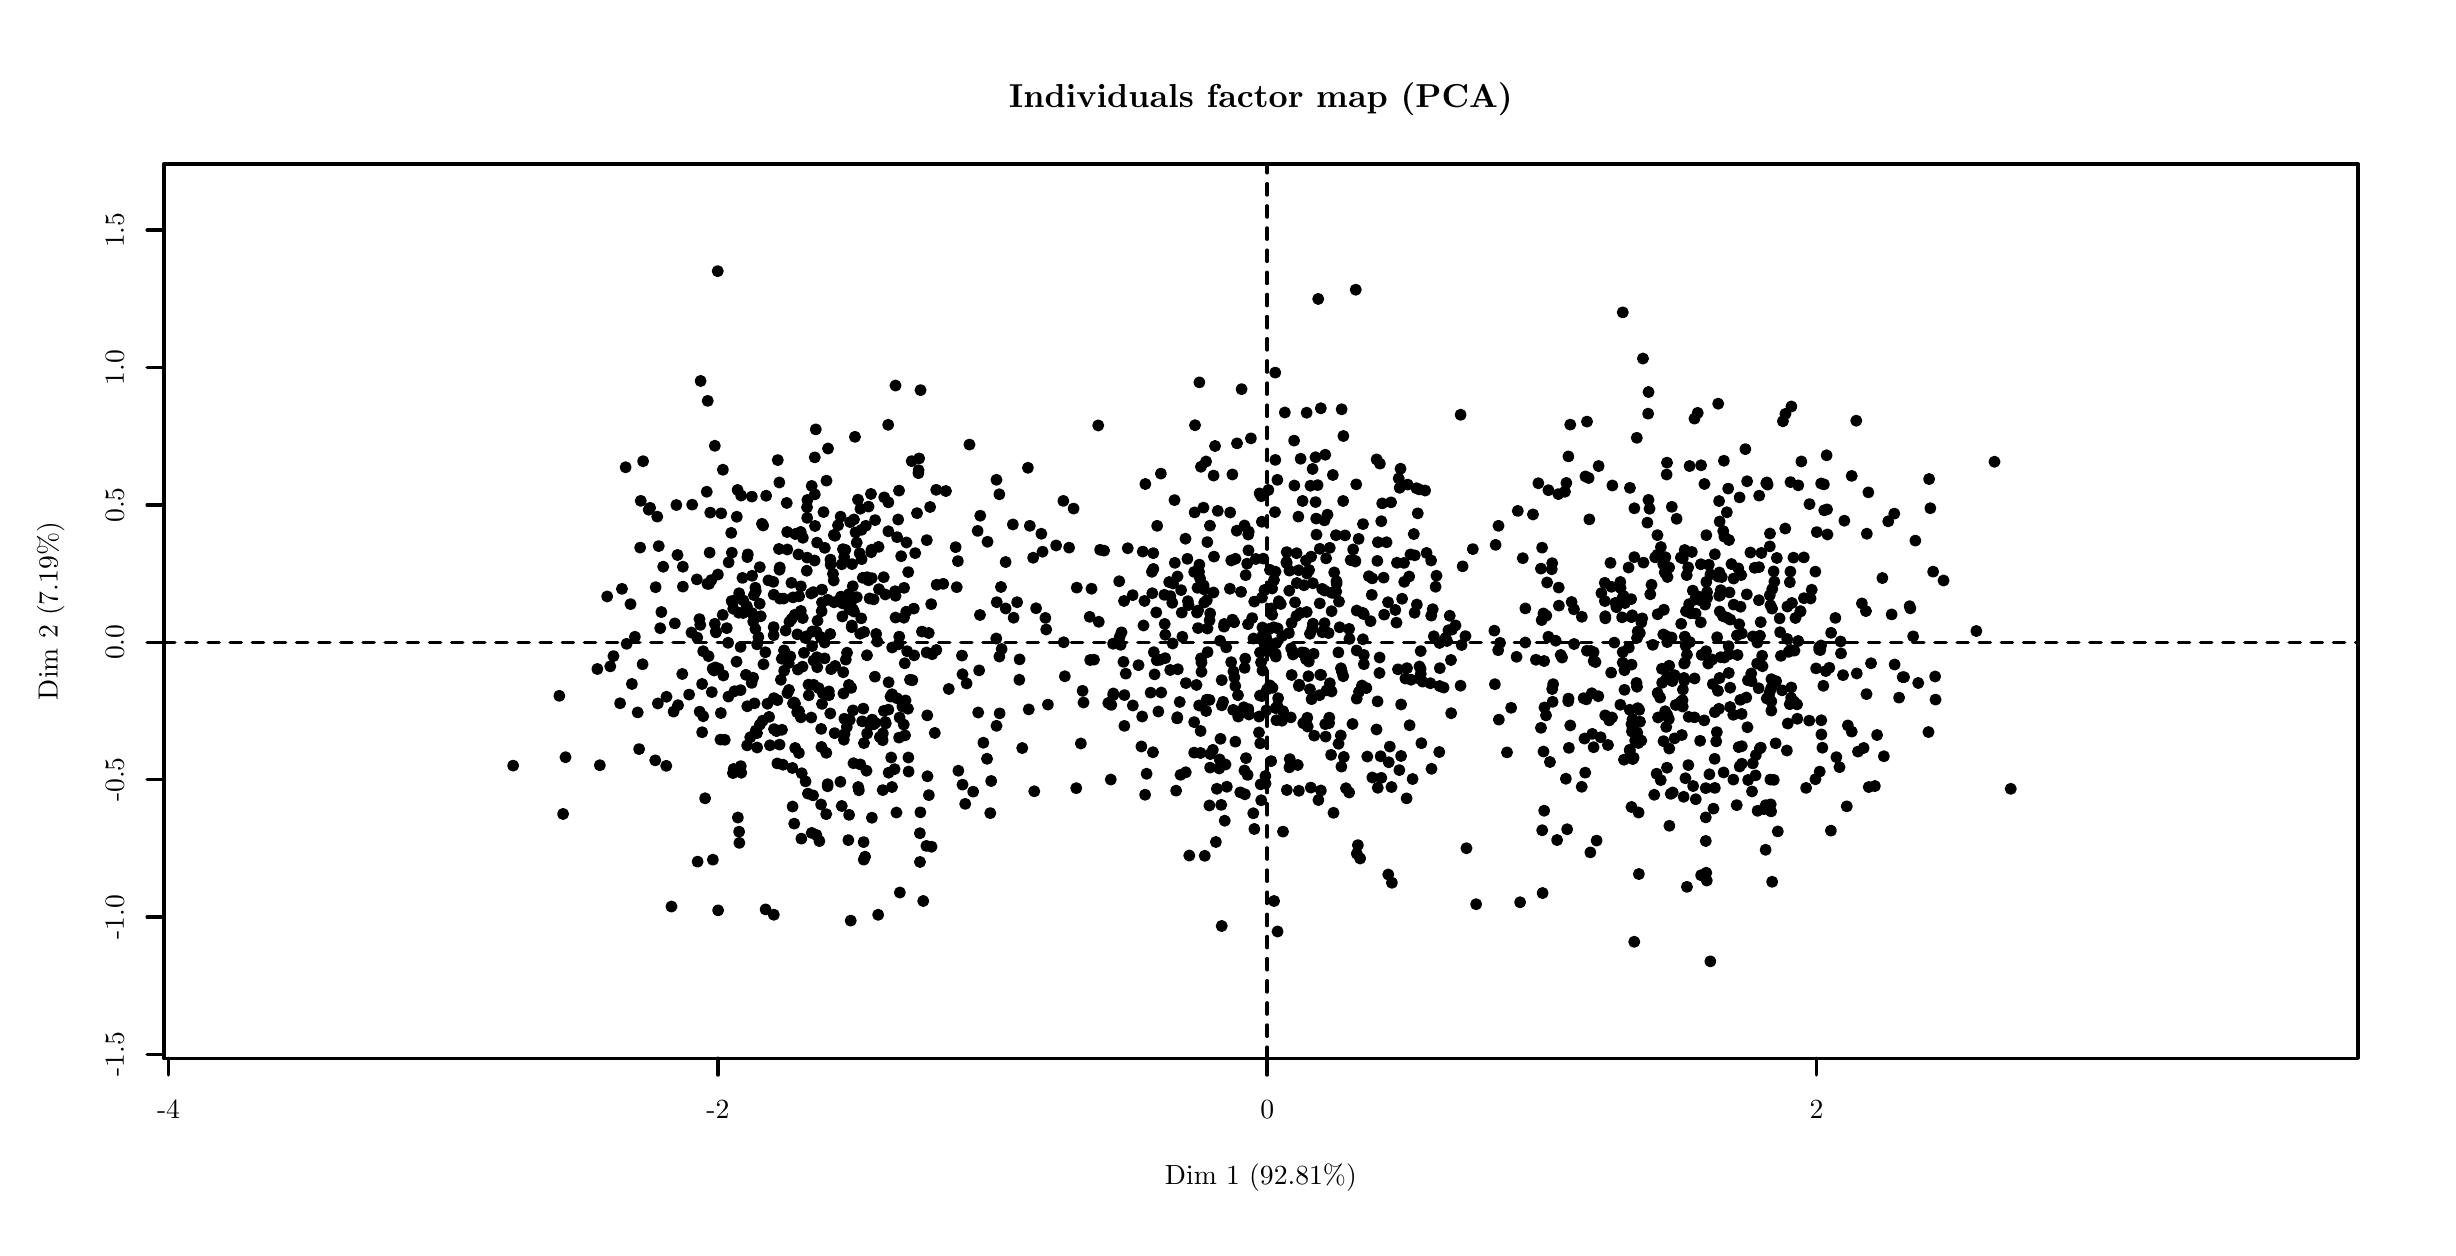
\begin{tikzpicture}[x=1pt,y=1pt]
\definecolor{fillColor}{RGB}{255,255,255}
\path[use as bounding box,fill=fillColor,fill opacity=0.00] (0,0) rectangle (867.24,433.62);
\begin{scope}
\path[clip] ( 49.20, 61.20) rectangle (842.04,384.42);
\definecolor{drawColor}{RGB}{255,255,255}

\path[draw=drawColor,line width= 1.3pt,line join=round,line cap=round] (447.91,211.52) circle (  2.25);
\end{scope}
\begin{scope}
\path[clip] (  0.00,  0.00) rectangle (867.24,433.62);
\definecolor{drawColor}{RGB}{0,0,0}

\path[draw=drawColor,line width= 1.3pt,line join=round,line cap=round] ( 50.90, 61.20) -- (646.41, 61.20);

\path[draw=drawColor,line width= 1.3pt,line join=round,line cap=round] ( 50.90, 61.20) -- ( 50.90, 55.20);

\path[draw=drawColor,line width= 1.3pt,line join=round,line cap=round] (249.40, 61.20) -- (249.40, 55.20);

\path[draw=drawColor,line width= 1.3pt,line join=round,line cap=round] (447.91, 61.20) -- (447.91, 55.20);

\path[draw=drawColor,line width= 1.3pt,line join=round,line cap=round] (646.41, 61.20) -- (646.41, 55.20);

\node[text=drawColor,anchor=base,inner sep=0pt, outer sep=0pt, scale=  1.00] at ( 50.90, 39.60) {-4};

\node[text=drawColor,anchor=base,inner sep=0pt, outer sep=0pt, scale=  1.00] at (249.40, 39.60) {-2};

\node[text=drawColor,anchor=base,inner sep=0pt, outer sep=0pt, scale=  1.00] at (447.91, 39.60) {0};

\node[text=drawColor,anchor=base,inner sep=0pt, outer sep=0pt, scale=  1.00] at (646.41, 39.60) {2};

\path[draw=drawColor,line width= 1.3pt,line join=round,line cap=round] ( 49.20, 62.64) -- ( 49.20,360.40);

\path[draw=drawColor,line width= 1.3pt,line join=round,line cap=round] ( 49.20, 62.64) -- ( 43.20, 62.64);

\path[draw=drawColor,line width= 1.3pt,line join=round,line cap=round] ( 49.20,112.27) -- ( 43.20,112.27);

\path[draw=drawColor,line width= 1.3pt,line join=round,line cap=round] ( 49.20,161.89) -- ( 43.20,161.89);

\path[draw=drawColor,line width= 1.3pt,line join=round,line cap=round] ( 49.20,211.52) -- ( 43.20,211.52);

\path[draw=drawColor,line width= 1.3pt,line join=round,line cap=round] ( 49.20,261.14) -- ( 43.20,261.14);

\path[draw=drawColor,line width= 1.3pt,line join=round,line cap=round] ( 49.20,310.77) -- ( 43.20,310.77);

\path[draw=drawColor,line width= 1.3pt,line join=round,line cap=round] ( 49.20,360.40) -- ( 43.20,360.40);

\node[text=drawColor,rotate= 90.00,anchor=base,inner sep=0pt, outer sep=0pt, scale=  1.00] at ( 34.80, 62.64) {-1.5};

\node[text=drawColor,rotate= 90.00,anchor=base,inner sep=0pt, outer sep=0pt, scale=  1.00] at ( 34.80,112.27) {-1.0};

\node[text=drawColor,rotate= 90.00,anchor=base,inner sep=0pt, outer sep=0pt, scale=  1.00] at ( 34.80,161.89) {-0.5};

\node[text=drawColor,rotate= 90.00,anchor=base,inner sep=0pt, outer sep=0pt, scale=  1.00] at ( 34.80,211.52) {0.0};

\node[text=drawColor,rotate= 90.00,anchor=base,inner sep=0pt, outer sep=0pt, scale=  1.00] at ( 34.80,261.14) {0.5};

\node[text=drawColor,rotate= 90.00,anchor=base,inner sep=0pt, outer sep=0pt, scale=  1.00] at ( 34.80,310.77) {1.0};

\node[text=drawColor,rotate= 90.00,anchor=base,inner sep=0pt, outer sep=0pt, scale=  1.00] at ( 34.80,360.40) {1.5};

\path[draw=drawColor,line width= 1.3pt,line join=round,line cap=round] ( 49.20, 61.20) --
	(842.04, 61.20) --
	(842.04,384.42) --
	( 49.20,384.42) --
	( 49.20, 61.20);
\end{scope}
\begin{scope}
\path[clip] (  0.00,  0.00) rectangle (867.24,433.62);
\definecolor{drawColor}{RGB}{0,0,0}

\node[text=drawColor,anchor=base,inner sep=0pt, outer sep=0pt, scale=  1.20] at (445.62,404.88) {\bfseries Individuals factor map (PCA)};

\node[text=drawColor,anchor=base,inner sep=0pt, outer sep=0pt, scale=  1.00] at (445.62, 15.60) {Dim 1 (92.81{\%})};

\node[text=drawColor,rotate= 90.00,anchor=base,inner sep=0pt, outer sep=0pt, scale=  1.00] at ( 10.80,222.81) {Dim 2 (7.19{\%})};
\end{scope}
\begin{scope}
\path[clip] ( 49.20, 61.20) rectangle (842.04,384.42);
\definecolor{drawColor}{RGB}{0,0,0}

\path[draw=drawColor,line width= 1.3pt,dash pattern=on 4pt off 4pt ,line join=round,line cap=round] (447.91, 61.20) -- (447.91,384.42);

\path[draw=drawColor,line width= 1.3pt,dash pattern=on 4pt off 4pt ,line join=round,line cap=round] ( 49.20,211.52) -- (842.04,211.52);
\definecolor{fillColor}{RGB}{0,0,0}

\path[draw=drawColor,line width= 1.3pt,line join=round,line cap=round,fill=fillColor] (440.98,218.07) circle (  1.50);

\path[draw=drawColor,line width= 1.3pt,line join=round,line cap=round,fill=fillColor] (509.07,235.58) circle (  1.50);

\path[draw=drawColor,line width= 1.3pt,line join=round,line cap=round,fill=fillColor] (311.00,251.63) circle (  1.50);

\path[draw=drawColor,line width= 1.3pt,line join=round,line cap=round,fill=fillColor] (337.81,160.08) circle (  1.50);

\path[draw=drawColor,line width= 1.3pt,line join=round,line cap=round,fill=fillColor] (379.09,231.27) circle (  1.50);

\path[draw=drawColor,line width= 1.3pt,line join=round,line cap=round,fill=fillColor] (449.69,230.97) circle (  1.50);

\path[draw=drawColor,line width= 1.3pt,line join=round,line cap=round,fill=fillColor] (313.59,304.30) circle (  1.50);

\path[draw=drawColor,line width= 1.3pt,line join=round,line cap=round,fill=fillColor] (678.01,198.92) circle (  1.50);

\path[draw=drawColor,line width= 1.3pt,line join=round,line cap=round,fill=fillColor] (313.25,165.68) circle (  1.50);

\path[draw=drawColor,line width= 1.3pt,line join=round,line cap=round,fill=fillColor] (650.04,279.09) circle (  1.50);

\path[draw=drawColor,line width= 1.3pt,line join=round,line cap=round,fill=fillColor] (523.40,116.88) circle (  1.50);

\path[draw=drawColor,line width= 1.3pt,line join=round,line cap=round,fill=fillColor] (294.16,152.37) circle (  1.50);

\path[draw=drawColor,line width= 1.3pt,line join=round,line cap=round,fill=fillColor] (621.43,180.82) circle (  1.50);

\path[draw=drawColor,line width= 1.3pt,line join=round,line cap=round,fill=fillColor] (576.36,207.97) circle (  1.50);

\path[draw=drawColor,line width= 1.3pt,line join=round,line cap=round,fill=fillColor] (446.74,208.78) circle (  1.50);

\path[draw=drawColor,line width= 1.3pt,line join=round,line cap=round,fill=fillColor] (309.93,182.73) circle (  1.50);

\path[draw=drawColor,line width= 1.3pt,line join=round,line cap=round,fill=fillColor] (324.75,137.94) circle (  1.50);

\path[draw=drawColor,line width= 1.3pt,line join=round,line cap=round,fill=fillColor] (598.12,194.45) circle (  1.50);

\path[draw=drawColor,line width= 1.3pt,line join=round,line cap=round,fill=fillColor] (255.09,165.73) circle (  1.50);

\path[draw=drawColor,line width= 1.3pt,line join=round,line cap=round,fill=fillColor] (463.36,214.61) circle (  1.50);

\path[draw=drawColor,line width= 1.3pt,line join=round,line cap=round,fill=fillColor] (300.81,214.63) circle (  1.50);

\path[draw=drawColor,line width= 1.3pt,line join=round,line cap=round,fill=fillColor] (230.83,191.83) circle (  1.50);

\path[draw=drawColor,line width= 1.3pt,line join=round,line cap=round,fill=fillColor] (286.83,173.69) circle (  1.50);

\path[draw=drawColor,line width= 1.3pt,line join=round,line cap=round,fill=fillColor] (481.07,193.64) circle (  1.50);

\path[draw=drawColor,line width= 1.3pt,line join=round,line cap=round,fill=fillColor] (538.01,206.27) circle (  1.50);

\path[draw=drawColor,line width= 1.3pt,line join=round,line cap=round,fill=fillColor] (284.01,196.16) circle (  1.50);

\path[draw=drawColor,line width= 1.3pt,line join=round,line cap=round,fill=fillColor] (396.80,200.19) circle (  1.50);

\path[draw=drawColor,line width= 1.3pt,line join=round,line cap=round,fill=fillColor] (628.02,152.65) circle (  1.50);

\path[draw=drawColor,line width= 1.3pt,line join=round,line cap=round,fill=fillColor] (440.12,235.79) circle (  1.50);

\path[draw=drawColor,line width= 1.3pt,line join=round,line cap=round,fill=fillColor] (322.42,132.15) circle (  1.50);

\path[draw=drawColor,line width= 1.3pt,line join=round,line cap=round,fill=fillColor] (193.46,149.50) circle (  1.50);

\path[draw=drawColor,line width= 1.3pt,line join=round,line cap=round,fill=fillColor] (278.32,201.67) circle (  1.50);

\path[draw=drawColor,line width= 1.3pt,line join=round,line cap=round,fill=fillColor] (636.00,182.16) circle (  1.50);

\path[draw=drawColor,line width= 1.3pt,line join=round,line cap=round,fill=fillColor] (624.92,203.82) circle (  1.50);

\path[draw=drawColor,line width= 1.3pt,line join=round,line cap=round,fill=fillColor] (483.75,194.99) circle (  1.50);

\path[draw=drawColor,line width= 1.3pt,line join=round,line cap=round,fill=fillColor] (670.73,170.34) circle (  1.50);

\path[draw=drawColor,line width= 1.3pt,line join=round,line cap=round,fill=fillColor] (286.69,152.93) circle (  1.50);

\path[draw=drawColor,line width= 1.3pt,line join=round,line cap=round,fill=fillColor] (267.92,184.56) circle (  1.50);

\path[draw=drawColor,line width= 1.3pt,line join=round,line cap=round,fill=fillColor] (501.98,225.16) circle (  1.50);

\path[draw=drawColor,line width= 1.3pt,line join=round,line cap=round,fill=fillColor] (451.17,211.23) circle (  1.50);

\path[draw=drawColor,line width= 1.3pt,line join=round,line cap=round,fill=fillColor] (304.92,244.96) circle (  1.50);

\path[draw=drawColor,line width= 1.3pt,line join=round,line cap=round,fill=fillColor] (553.23,231.30) circle (  1.50);

\path[draw=drawColor,line width= 1.3pt,line join=round,line cap=round,fill=fillColor] (249.41,236.00) circle (  1.50);

\path[draw=drawColor,line width= 1.3pt,line join=round,line cap=round,fill=fillColor] (643.86,261.46) circle (  1.50);

\path[draw=drawColor,line width= 1.3pt,line join=round,line cap=round,fill=fillColor] (501.21,242.95) circle (  1.50);

\path[draw=drawColor,line width= 1.3pt,line join=round,line cap=round,fill=fillColor] (602.51,226.99) circle (  1.50);

\path[draw=drawColor,line width= 1.3pt,line join=round,line cap=round,fill=fillColor] (629.83,152.97) circle (  1.50);

\path[draw=drawColor,line width= 1.3pt,line join=round,line cap=round,fill=fillColor] (251.14,221.42) circle (  1.50);

\path[draw=drawColor,line width= 1.3pt,line join=round,line cap=round,fill=fillColor] (611.23,228.32) circle (  1.50);

\path[draw=drawColor,line width= 1.3pt,line join=round,line cap=round,fill=fillColor] (406.38,229.25) circle (  1.50);

\path[draw=drawColor,line width= 1.3pt,line join=round,line cap=round,fill=fillColor] (455.88,230.17) circle (  1.50);

\path[draw=drawColor,line width= 1.3pt,line join=round,line cap=round,fill=fillColor] (644.65,230.51) circle (  1.50);

\path[draw=drawColor,line width= 1.3pt,line join=round,line cap=round,fill=fillColor] (285.17,206.14) circle (  1.50);

\path[draw=drawColor,line width= 1.3pt,line join=round,line cap=round,fill=fillColor] (590.09,161.72) circle (  1.50);

\path[draw=drawColor,line width= 1.3pt,line join=round,line cap=round,fill=fillColor] (472.14,229.35) circle (  1.50);

\path[draw=drawColor,line width= 1.3pt,line join=round,line cap=round,fill=fillColor] (460.68,262.59) circle (  1.50);

\path[draw=drawColor,line width= 1.3pt,line join=round,line cap=round,fill=fillColor] (436.42,241.70) circle (  1.50);

\path[draw=drawColor,line width= 1.3pt,line join=round,line cap=round,fill=fillColor] (445.38,175.01) circle (  1.50);

\path[draw=drawColor,line width= 1.3pt,line join=round,line cap=round,fill=fillColor] (487.40,180.03) circle (  1.50);

\path[draw=drawColor,line width= 1.3pt,line join=round,line cap=round,fill=fillColor] (258.55,222.12) circle (  1.50);

\path[draw=drawColor,line width= 1.3pt,line join=round,line cap=round,fill=fillColor] (367.75,220.33) circle (  1.50);

\path[draw=drawColor,line width= 1.3pt,line join=round,line cap=round,fill=fillColor] (450.93,207.34) circle (  1.50);

\path[draw=drawColor,line width= 1.3pt,line join=round,line cap=round,fill=fillColor] (224.91,260.10) circle (  1.50);

\path[draw=drawColor,line width= 1.3pt,line join=round,line cap=round,fill=fillColor] (566.52,204.37) circle (  1.50);

\path[draw=drawColor,line width= 1.3pt,line join=round,line cap=round,fill=fillColor] (450.35,234.01) circle (  1.50);

\path[draw=drawColor,line width= 1.3pt,line join=round,line cap=round,fill=fillColor] (635.79,212.73) circle (  1.50);

\path[draw=drawColor,line width= 1.3pt,line join=round,line cap=round,fill=fillColor] (547.98,150.67) circle (  1.50);

\path[draw=drawColor,line width= 1.3pt,line join=round,line cap=round,fill=fillColor] (570.05,220.93) circle (  1.50);

\path[draw=drawColor,line width= 1.3pt,line join=round,line cap=round,fill=fillColor] (209.40,228.09) circle (  1.50);

\path[draw=drawColor,line width= 1.3pt,line join=round,line cap=round,fill=fillColor] (604.60,239.72) circle (  1.50);

\path[draw=drawColor,line width= 1.3pt,line join=round,line cap=round,fill=fillColor] (283.30,268.03) circle (  1.50);

\path[draw=drawColor,line width= 1.3pt,line join=round,line cap=round,fill=fillColor] (248.30,282.53) circle (  1.50);

\path[draw=drawColor,line width= 1.3pt,line join=round,line cap=round,fill=fillColor] (591.11,175.79) circle (  1.50);

\path[draw=drawColor,line width= 1.3pt,line join=round,line cap=round,fill=fillColor] (262.63,189.47) circle (  1.50);

\path[draw=drawColor,line width= 1.3pt,line join=round,line cap=round,fill=fillColor] (260.23,243.31) circle (  1.50);

\path[draw=drawColor,line width= 1.3pt,line join=round,line cap=round,fill=fillColor] (626.48,243.81) circle (  1.50);

\path[draw=drawColor,line width= 1.3pt,line join=round,line cap=round,fill=fillColor] (648.03,210.37) circle (  1.50);

\path[draw=drawColor,line width= 1.3pt,line join=round,line cap=round,fill=fillColor] (274.49,245.05) circle (  1.50);

\path[draw=drawColor,line width= 1.3pt,line join=round,line cap=round,fill=fillColor] (258.29,234.79) circle (  1.50);

\path[draw=drawColor,line width= 1.3pt,line join=round,line cap=round,fill=fillColor] (576.37,204.18) circle (  1.50);

\path[draw=drawColor,line width= 1.3pt,line join=round,line cap=round,fill=fillColor] (484.63,235.40) circle (  1.50);

\path[draw=drawColor,line width= 1.3pt,line join=round,line cap=round,fill=fillColor] (270.92,190.62) circle (  1.50);

\path[draw=drawColor,line width= 1.3pt,line join=round,line cap=round,fill=fillColor] (626.73,206.66) circle (  1.50);

\path[draw=drawColor,line width= 1.3pt,line join=round,line cap=round,fill=fillColor] (572.28,231.57) circle (  1.50);

\path[draw=drawColor,line width= 1.3pt,line join=round,line cap=round,fill=fillColor] (473.84,226.23) circle (  1.50);

\path[draw=drawColor,line width= 1.3pt,line join=round,line cap=round,fill=fillColor] (600.52,275.21) circle (  1.50);

\path[draw=drawColor,line width= 1.3pt,line join=round,line cap=round,fill=fillColor] (489.13,162.55) circle (  1.50);

\path[draw=drawColor,line width= 1.3pt,line join=round,line cap=round,fill=fillColor] (479.72,240.73) circle (  1.50);

\path[draw=drawColor,line width= 1.3pt,line join=round,line cap=round,fill=fillColor] (554.44,206.01) circle (  1.50);

\path[draw=drawColor,line width= 1.3pt,line join=round,line cap=round,fill=fillColor] (599.11,210.27) circle (  1.50);

\path[draw=drawColor,line width= 1.3pt,line join=round,line cap=round,fill=fillColor] (269.43,233.37) circle (  1.50);

\path[draw=drawColor,line width= 1.3pt,line join=round,line cap=round,fill=fillColor] (431.46,109.01) circle (  1.50);

\path[draw=drawColor,line width= 1.3pt,line join=round,line cap=round,fill=fillColor] (597.49,218.21) circle (  1.50);

\path[draw=drawColor,line width= 1.3pt,line join=round,line cap=round,fill=fillColor] (463.34,194.55) circle (  1.50);

\path[draw=drawColor,line width= 1.3pt,line join=round,line cap=round,fill=fillColor] (296.95,223.47) circle (  1.50);

\path[draw=drawColor,line width= 1.3pt,line join=round,line cap=round,fill=fillColor] (435.33,272.17) circle (  1.50);

\path[draw=drawColor,line width= 1.3pt,line join=round,line cap=round,fill=fillColor] (600.95,222.01) circle (  1.50);

\path[draw=drawColor,line width= 1.3pt,line join=round,line cap=round,fill=fillColor] (300.60,243.69) circle (  1.50);

\path[draw=drawColor,line width= 1.3pt,line join=round,line cap=round,fill=fillColor] (502.30,258.12) circle (  1.50);

\path[draw=drawColor,line width= 1.3pt,line join=round,line cap=round,fill=fillColor] (503.61,175.07) circle (  1.50);

\path[draw=drawColor,line width= 1.3pt,line join=round,line cap=round,fill=fillColor] (586.06,259.78) circle (  1.50);

\path[draw=drawColor,line width= 1.3pt,line join=round,line cap=round,fill=fillColor] (247.21,193.52) circle (  1.50);

\path[draw=drawColor,line width= 1.3pt,line join=round,line cap=round,fill=fillColor] (246.66,258.39) circle (  1.50);

\path[draw=drawColor,line width= 1.3pt,line join=round,line cap=round,fill=fillColor] (480.23,208.58) circle (  1.50);

\path[draw=drawColor,line width= 1.3pt,line join=round,line cap=round,fill=fillColor] (234.41,261.12) circle (  1.50);

\path[draw=drawColor,line width= 1.3pt,line join=round,line cap=round,fill=fillColor] (459.29,237.56) circle (  1.50);

\path[draw=drawColor,line width= 1.3pt,line join=round,line cap=round,fill=fillColor] (552.15,212.10) circle (  1.50);

\path[draw=drawColor,line width= 1.3pt,line join=round,line cap=round,fill=fillColor] (565.86,207.93) circle (  1.50);

\path[draw=drawColor,line width= 1.3pt,line join=round,line cap=round,fill=fillColor] (651.65,214.94) circle (  1.50);

\path[draw=drawColor,line width= 1.3pt,line join=round,line cap=round,fill=fillColor] (351.13,206.37) circle (  1.50);

\path[draw=drawColor,line width= 1.3pt,line join=round,line cap=round,fill=fillColor] (630.33,223.68) circle (  1.50);

\path[draw=drawColor,line width= 1.3pt,line join=round,line cap=round,fill=fillColor] (639.78,211.99) circle (  1.50);

\path[draw=drawColor,line width= 1.3pt,line join=round,line cap=round,fill=fillColor] (320.70,243.75) circle (  1.50);

\path[draw=drawColor,line width= 1.3pt,line join=round,line cap=round,fill=fillColor] (531.61,183.58) circle (  1.50);

\path[draw=drawColor,line width= 1.3pt,line join=round,line cap=round,fill=fillColor] (249.49,114.66) circle (  1.50);

\path[draw=drawColor,line width= 1.3pt,line join=round,line cap=round,fill=fillColor] (312.34,192.74) circle (  1.50);

\path[draw=drawColor,line width= 1.3pt,line join=round,line cap=round,fill=fillColor] (312.31,159.22) circle (  1.50);

\path[draw=drawColor,line width= 1.3pt,line join=round,line cap=round,fill=fillColor] (294.80,193.03) circle (  1.50);

\path[draw=drawColor,line width= 1.3pt,line join=round,line cap=round,fill=fillColor] (494.20,223.21) circle (  1.50);

\path[draw=drawColor,line width= 1.3pt,line join=round,line cap=round,fill=fillColor] (504.97,266.36) circle (  1.50);

\path[draw=drawColor,line width= 1.3pt,line join=round,line cap=round,fill=fillColor] (301.36,241.58) circle (  1.50);

\path[draw=drawColor,line width= 1.3pt,line join=round,line cap=round,fill=fillColor] (447.29,160.47) circle (  1.50);

\path[draw=drawColor,line width= 1.3pt,line join=round,line cap=round,fill=fillColor] (210.53,202.82) circle (  1.50);

\path[draw=drawColor,line width= 1.3pt,line join=round,line cap=round,fill=fillColor] (413.74,211.09) circle (  1.50);

\path[draw=drawColor,line width= 1.3pt,line join=round,line cap=round,fill=fillColor] (211.67,206.54) circle (  1.50);

\path[draw=drawColor,line width= 1.3pt,line join=round,line cap=round,fill=fillColor] (451.58,270.22) circle (  1.50);

\path[draw=drawColor,line width= 1.3pt,line join=round,line cap=round,fill=fillColor] (485.88,162.67) circle (  1.50);

\path[draw=drawColor,line width= 1.3pt,line join=round,line cap=round,fill=fillColor] (348.16,161.40) circle (  1.50);

\path[draw=drawColor,line width= 1.3pt,line join=round,line cap=round,fill=fillColor] (258.59,226.64) circle (  1.50);

\path[draw=drawColor,line width= 1.3pt,line join=round,line cap=round,fill=fillColor] (368.04,216.15) circle (  1.50);

\path[draw=drawColor,line width= 1.3pt,line join=round,line cap=round,fill=fillColor] (704.14,215.60) circle (  1.50);

\path[draw=drawColor,line width= 1.3pt,line join=round,line cap=round,fill=fillColor] (422.34,196.11) circle (  1.50);

\path[draw=drawColor,line width= 1.3pt,line join=round,line cap=round,fill=fillColor] (632.06,241.99) circle (  1.50);

\path[draw=drawColor,line width= 1.3pt,line join=round,line cap=round,fill=fillColor] (566.94,139.88) circle (  1.50);

\path[draw=drawColor,line width= 1.3pt,line join=round,line cap=round,fill=fillColor] (205.85,201.87) circle (  1.50);

\path[draw=drawColor,line width= 1.3pt,line join=round,line cap=round,fill=fillColor] (495.77,267.35) circle (  1.50);

\path[draw=drawColor,line width= 1.3pt,line join=round,line cap=round,fill=fillColor] (259.90,224.10) circle (  1.50);

\path[draw=drawColor,line width= 1.3pt,line join=round,line cap=round,fill=fillColor] (313.60,228.33) circle (  1.50);

\path[draw=drawColor,line width= 1.3pt,line join=round,line cap=round,fill=fillColor] (659.10,271.65) circle (  1.50);

\path[draw=drawColor,line width= 1.3pt,line join=round,line cap=round,fill=fillColor] (561.59,220.74) circle (  1.50);

\path[draw=drawColor,line width= 1.3pt,line join=round,line cap=round,fill=fillColor] (214.06,189.49) circle (  1.50);

\path[draw=drawColor,line width= 1.3pt,line join=round,line cap=round,fill=fillColor] (399.29,228.57) circle (  1.50);

\path[draw=drawColor,line width= 1.3pt,line join=round,line cap=round,fill=fillColor] (617.55,152.68) circle (  1.50);

\path[draw=drawColor,line width= 1.3pt,line join=round,line cap=round,fill=fillColor] (598.76,244.87) circle (  1.50);

\path[draw=drawColor,line width= 1.3pt,line join=round,line cap=round,fill=fillColor] (583.67,314.05) circle (  1.50);

\path[draw=drawColor,line width= 1.3pt,line join=round,line cap=round,fill=fillColor] (314.55,255.88) circle (  1.50);

\path[draw=drawColor,line width= 1.3pt,line join=round,line cap=round,fill=fillColor] (563.46,291.28) circle (  1.50);

\path[draw=drawColor,line width= 1.3pt,line join=round,line cap=round,fill=fillColor] (444.92,178.93) circle (  1.50);

\path[draw=drawColor,line width= 1.3pt,line join=round,line cap=round,fill=fillColor] (423.80,171.53) circle (  1.50);

\path[draw=drawColor,line width= 1.3pt,line join=round,line cap=round,fill=fillColor] (407.21,199.93) circle (  1.50);

\path[draw=drawColor,line width= 1.3pt,line join=round,line cap=round,fill=fillColor] (446.91,230.41) circle (  1.50);

\path[draw=drawColor,line width= 1.3pt,line join=round,line cap=round,fill=fillColor] (635.09,252.63) circle (  1.50);

\path[draw=drawColor,line width= 1.3pt,line join=round,line cap=round,fill=fillColor] (563.21,190.90) circle (  1.50);

\path[draw=drawColor,line width= 1.3pt,line join=round,line cap=round,fill=fillColor] (465.37,262.19) circle (  1.50);

\path[draw=drawColor,line width= 1.3pt,line join=round,line cap=round,fill=fillColor] (440.82,163.60) circle (  1.50);

\path[draw=drawColor,line width= 1.3pt,line join=round,line cap=round,fill=fillColor] (451.00,206.34) circle (  1.50);

\path[draw=drawColor,line width= 1.3pt,line join=round,line cap=round,fill=fillColor] (431.02,176.64) circle (  1.50);

\path[draw=drawColor,line width= 1.3pt,line join=round,line cap=round,fill=fillColor] (298.57,255.91) circle (  1.50);

\path[draw=drawColor,line width= 1.3pt,line join=round,line cap=round,fill=fillColor] (615.16,188.13) circle (  1.50);

\path[draw=drawColor,line width= 1.3pt,line join=round,line cap=round,fill=fillColor] (630.07,190.17) circle (  1.50);

\path[draw=drawColor,line width= 1.3pt,line join=round,line cap=round,fill=fillColor] (581.80,187.73) circle (  1.50);

\path[draw=drawColor,line width= 1.3pt,line join=round,line cap=round,fill=fillColor] (266.85,264.48) circle (  1.50);

\path[draw=drawColor,line width= 1.3pt,line join=round,line cap=round,fill=fillColor] (546.81,238.15) circle (  1.50);

\path[draw=drawColor,line width= 1.3pt,line join=round,line cap=round,fill=fillColor] (281.52,237.39) circle (  1.50);

\path[draw=drawColor,line width= 1.3pt,line join=round,line cap=round,fill=fillColor] (643.75,183.21) circle (  1.50);

\path[draw=drawColor,line width= 1.3pt,line join=round,line cap=round,fill=fillColor] (680.03,224.57) circle (  1.50);

\path[draw=drawColor,line width= 1.3pt,line join=round,line cap=round,fill=fillColor] (454.95,244.11) circle (  1.50);

\path[draw=drawColor,line width= 1.3pt,line join=round,line cap=round,fill=fillColor] (440.64,239.92) circle (  1.50);

\path[draw=drawColor,line width= 1.3pt,line join=round,line cap=round,fill=fillColor] (638.06,242.10) circle (  1.50);

\path[draw=drawColor,line width= 1.3pt,line join=round,line cap=round,fill=fillColor] (315.16,121.10) circle (  1.50);

\path[draw=drawColor,line width= 1.3pt,line join=round,line cap=round,fill=fillColor] (450.38,118.03) circle (  1.50);

\path[draw=drawColor,line width= 1.3pt,line join=round,line cap=round,fill=fillColor] (609.15,151.41) circle (  1.50);

\path[draw=drawColor,line width= 1.3pt,line join=round,line cap=round,fill=fillColor] (598.82,204.22) circle (  1.50);

\path[draw=drawColor,line width= 1.3pt,line join=round,line cap=round,fill=fillColor] (611.79,230.36) circle (  1.50);

\path[draw=drawColor,line width= 1.3pt,line join=round,line cap=round,fill=fillColor] (450.27,216.94) circle (  1.50);

\path[draw=drawColor,line width= 1.3pt,line join=round,line cap=round,fill=fillColor] (680.31,223.78) circle (  1.50);

\path[draw=drawColor,line width= 1.3pt,line join=round,line cap=round,fill=fillColor] (301.30,252.16) circle (  1.50);

\path[draw=drawColor,line width= 1.3pt,line join=round,line cap=round,fill=fillColor] (604.68,275.48) circle (  1.50);

\path[draw=drawColor,line width= 1.3pt,line join=round,line cap=round,fill=fillColor] (281.95,156.85) circle (  1.50);

\path[draw=drawColor,line width= 1.3pt,line join=round,line cap=round,fill=fillColor] (456.41,184.39) circle (  1.50);

\path[draw=drawColor,line width= 1.3pt,line join=round,line cap=round,fill=fillColor] (581.62,178.85) circle (  1.50);

\path[draw=drawColor,line width= 1.3pt,line join=round,line cap=round,fill=fillColor] (280.12,249.29) circle (  1.50);

\path[draw=drawColor,line width= 1.3pt,line join=round,line cap=round,fill=fillColor] (309.39,186.74) circle (  1.50);

\path[draw=drawColor,line width= 1.3pt,line join=round,line cap=round,fill=fillColor] (446.58,211.74) circle (  1.50);

\path[draw=drawColor,line width= 1.3pt,line join=round,line cap=round,fill=fillColor] (416.59,163.63) circle (  1.50);

\path[draw=drawColor,line width= 1.3pt,line join=round,line cap=round,fill=fillColor] (327.79,178.77) circle (  1.50);

\path[draw=drawColor,line width= 1.3pt,line join=round,line cap=round,fill=fillColor] (428.53,271.77) circle (  1.50);

\path[draw=drawColor,line width= 1.3pt,line join=round,line cap=round,fill=fillColor] (606.84,229.67) circle (  1.50);

\path[draw=drawColor,line width= 1.3pt,line join=round,line cap=round,fill=fillColor] (567.66,275.21) circle (  1.50);

\path[draw=drawColor,line width= 1.3pt,line join=round,line cap=round,fill=fillColor] (391.37,161.93) circle (  1.50);

\path[draw=drawColor,line width= 1.3pt,line join=round,line cap=round,fill=fillColor] (577.01,194.34) circle (  1.50);

\path[draw=drawColor,line width= 1.3pt,line join=round,line cap=round,fill=fillColor] (266.64,115.01) circle (  1.50);

\path[draw=drawColor,line width= 1.3pt,line join=round,line cap=round,fill=fillColor] (459.81,222.10) circle (  1.50);

\path[draw=drawColor,line width= 1.3pt,line join=round,line cap=round,fill=fillColor] (421.50,171.65) circle (  1.50);

\path[draw=drawColor,line width= 1.3pt,line join=round,line cap=round,fill=fillColor] (496.07,274.24) circle (  1.50);

\path[draw=drawColor,line width= 1.3pt,line join=round,line cap=round,fill=fillColor] (397.51,245.51) circle (  1.50);

\path[draw=drawColor,line width= 1.3pt,line join=round,line cap=round,fill=fillColor] (350.08,181.34) circle (  1.50);

\path[draw=drawColor,line width= 1.3pt,line join=round,line cap=round,fill=fillColor] (562.56,176.74) circle (  1.50);

\path[draw=drawColor,line width= 1.3pt,line join=round,line cap=round,fill=fillColor] (491.03,247.67) circle (  1.50);

\path[draw=drawColor,line width= 1.3pt,line join=round,line cap=round,fill=fillColor] (501.82,267.19) circle (  1.50);

\path[draw=drawColor,line width= 1.3pt,line join=round,line cap=round,fill=fillColor] (587.23,210.61) circle (  1.50);

\path[draw=drawColor,line width= 1.3pt,line join=round,line cap=round,fill=fillColor] (471.18,229.44) circle (  1.50);

\path[draw=drawColor,line width= 1.3pt,line join=round,line cap=round,fill=fillColor] (459.17,256.92) circle (  1.50);

\path[draw=drawColor,line width= 1.3pt,line join=round,line cap=round,fill=fillColor] (613.08,249.69) circle (  1.50);

\path[draw=drawColor,line width= 1.3pt,line join=round,line cap=round,fill=fillColor] (294.14,239.71) circle (  1.50);

\path[draw=drawColor,line width= 1.3pt,line join=round,line cap=round,fill=fillColor] (591.03,214.36) circle (  1.50);

\path[draw=drawColor,line width= 1.3pt,line join=round,line cap=round,fill=fillColor] (519.90,137.11) circle (  1.50);

\path[draw=drawColor,line width= 1.3pt,line join=round,line cap=round,fill=fillColor] (590.52,201.96) circle (  1.50);

\path[draw=drawColor,line width= 1.3pt,line join=round,line cap=round,fill=fillColor] (439.83,156.60) circle (  1.50);

\path[draw=drawColor,line width= 1.3pt,line join=round,line cap=round,fill=fillColor] (328.30,266.62) circle (  1.50);

\path[draw=drawColor,line width= 1.3pt,line join=round,line cap=round,fill=fillColor] (578.93,172.33) circle (  1.50);

\path[draw=drawColor,line width= 1.3pt,line join=round,line cap=round,fill=fillColor] (628.00,136.55) circle (  1.50);

\path[draw=drawColor,line width= 1.3pt,line join=round,line cap=round,fill=fillColor] (396.29,181.31) circle (  1.50);

\path[draw=drawColor,line width= 1.3pt,line join=round,line cap=round,fill=fillColor] (611.13,187.49) circle (  1.50);

\path[draw=drawColor,line width= 1.3pt,line join=round,line cap=round,fill=fillColor] (299.15,251.25) circle (  1.50);

\path[draw=drawColor,line width= 1.3pt,line join=round,line cap=round,fill=fillColor] (411.02,205.79) circle (  1.50);

\path[draw=drawColor,line width= 1.3pt,line join=round,line cap=round,fill=fillColor] (494.78,240.26) circle (  1.50);

\path[draw=drawColor,line width= 1.3pt,line join=round,line cap=round,fill=fillColor] (464.13,216.46) circle (  1.50);

\path[draw=drawColor,line width= 1.3pt,line join=round,line cap=round,fill=fillColor] (445.96,255.09) circle (  1.50);

\path[draw=drawColor,line width= 1.3pt,line join=round,line cap=round,fill=fillColor] (443.26,144.07) circle (  1.50);

\path[draw=drawColor,line width= 1.3pt,line join=round,line cap=round,fill=fillColor] (443.76,241.63) circle (  1.50);

\path[draw=drawColor,line width= 1.3pt,line join=round,line cap=round,fill=fillColor] (599.57,207.02) circle (  1.50);

\path[draw=drawColor,line width= 1.3pt,line join=round,line cap=round,fill=fillColor] (242.82,186.46) circle (  1.50);

\path[draw=drawColor,line width= 1.3pt,line join=round,line cap=round,fill=fillColor] (320.32,206.80) circle (  1.50);

\path[draw=drawColor,line width= 1.3pt,line join=round,line cap=round,fill=fillColor] (503.39,200.10) circle (  1.50);

\path[draw=drawColor,line width= 1.3pt,line join=round,line cap=round,fill=fillColor] (442.95,212.89) circle (  1.50);

\path[draw=drawColor,line width= 1.3pt,line join=round,line cap=round,fill=fillColor] (466.12,268.32) circle (  1.50);

\path[draw=drawColor,line width= 1.3pt,line join=round,line cap=round,fill=fillColor] (647.75,208.71) circle (  1.50);

\path[draw=drawColor,line width= 1.3pt,line join=round,line cap=round,fill=fillColor] (256.24,256.88) circle (  1.50);

\path[draw=drawColor,line width= 1.3pt,line join=round,line cap=round,fill=fillColor] (275.08,194.31) circle (  1.50);

\path[draw=drawColor,line width= 1.3pt,line join=round,line cap=round,fill=fillColor] (609.66,186.28) circle (  1.50);

\path[draw=drawColor,line width= 1.3pt,line join=round,line cap=round,fill=fillColor] (283.98,204.91) circle (  1.50);

\path[draw=drawColor,line width= 1.3pt,line join=round,line cap=round,fill=fillColor] (431.46,197.86) circle (  1.50);

\path[draw=drawColor,line width= 1.3pt,line join=round,line cap=round,fill=fillColor] (247.50,201.99) circle (  1.50);

\path[draw=drawColor,line width= 1.3pt,line join=round,line cap=round,fill=fillColor] (609.67,243.33) circle (  1.50);

\path[draw=drawColor,line width= 1.3pt,line join=round,line cap=round,fill=fillColor] (565.86,204.78) circle (  1.50);

\path[draw=drawColor,line width= 1.3pt,line join=round,line cap=round,fill=fillColor] (572.63,268.18) circle (  1.50);

\path[draw=drawColor,line width= 1.3pt,line join=round,line cap=round,fill=fillColor] (339.28,196.65) circle (  1.50);

\path[draw=drawColor,line width= 1.3pt,line join=round,line cap=round,fill=fillColor] (489.46,261.71) circle (  1.50);

\path[draw=drawColor,line width= 1.3pt,line join=round,line cap=round,fill=fillColor] (499.68,243.27) circle (  1.50);

\path[draw=drawColor,line width= 1.3pt,line join=round,line cap=round,fill=fillColor] (264.56,181.76) circle (  1.50);

\path[draw=drawColor,line width= 1.3pt,line join=round,line cap=round,fill=fillColor] (303.28,206.83) circle (  1.50);

\path[draw=drawColor,line width= 1.3pt,line join=round,line cap=round,fill=fillColor] (392.20,211.02) circle (  1.50);

\path[draw=drawColor,line width= 1.3pt,line join=round,line cap=round,fill=fillColor] (605.81,183.30) circle (  1.50);

\path[draw=drawColor,line width= 1.3pt,line join=round,line cap=round,fill=fillColor] (302.85,253.61) circle (  1.50);

\path[draw=drawColor,line width= 1.3pt,line join=round,line cap=round,fill=fillColor] (224.40,259.44) circle (  1.50);

\path[draw=drawColor,line width= 1.3pt,line join=round,line cap=round,fill=fillColor] (448.91,237.68) circle (  1.50);

\path[draw=drawColor,line width= 1.3pt,line join=round,line cap=round,fill=fillColor] (645.98,237.06) circle (  1.50);

\path[draw=drawColor,line width= 1.3pt,line join=round,line cap=round,fill=fillColor] (425.80,276.85) circle (  1.50);

\path[draw=drawColor,line width= 1.3pt,line join=round,line cap=round,fill=fillColor] (395.96,204.46) circle (  1.50);

\path[draw=drawColor,line width= 1.3pt,line join=round,line cap=round,fill=fillColor] (547.97,204.75) circle (  1.50);

\path[draw=drawColor,line width= 1.3pt,line join=round,line cap=round,fill=fillColor] (589.87,191.53) circle (  1.50);

\path[draw=drawColor,line width= 1.3pt,line join=round,line cap=round,fill=fillColor] (362.13,253.61) circle (  1.50);

\path[draw=drawColor,line width= 1.3pt,line join=round,line cap=round,fill=fillColor] (387.04,218.93) circle (  1.50);

\path[draw=drawColor,line width= 1.3pt,line join=round,line cap=round,fill=fillColor] (261.61,196.85) circle (  1.50);

\path[draw=drawColor,line width= 1.3pt,line join=round,line cap=round,fill=fillColor] (419.48,224.97) circle (  1.50);

\path[draw=drawColor,line width= 1.3pt,line join=round,line cap=round,fill=fillColor] (492.21,173.84) circle (  1.50);

\path[draw=drawColor,line width= 1.3pt,line join=round,line cap=round,fill=fillColor] (451.62,188.46) circle (  1.50);

\path[draw=drawColor,line width= 1.3pt,line join=round,line cap=round,fill=fillColor] (297.40,110.95) circle (  1.50);

\path[draw=drawColor,line width= 1.3pt,line join=round,line cap=round,fill=fillColor] (264.89,220.93) circle (  1.50);

\path[draw=drawColor,line width= 1.3pt,line join=round,line cap=round,fill=fillColor] (247.04,234.01) circle (  1.50);

\path[draw=drawColor,line width= 1.3pt,line join=round,line cap=round,fill=fillColor] (582.21,127.79) circle (  1.50);

\path[draw=drawColor,line width= 1.3pt,line join=round,line cap=round,fill=fillColor] (630.96,161.80) circle (  1.50);

\path[draw=drawColor,line width= 1.3pt,line join=round,line cap=round,fill=fillColor] (482.77,221.73) circle (  1.50);

\path[draw=drawColor,line width= 1.3pt,line join=round,line cap=round,fill=fillColor] (573.33,211.42) circle (  1.50);

\path[draw=drawColor,line width= 1.3pt,line join=round,line cap=round,fill=fillColor] (448.34,266.55) circle (  1.50);

\path[draw=drawColor,line width= 1.3pt,line join=round,line cap=round,fill=fillColor] (257.62,194.25) circle (  1.50);

\path[draw=drawColor,line width= 1.3pt,line join=round,line cap=round,fill=fillColor] (618.25,173.65) circle (  1.50);

\path[draw=drawColor,line width= 1.3pt,line join=round,line cap=round,fill=fillColor] (629.52,246.18) circle (  1.50);

\path[draw=drawColor,line width= 1.3pt,line join=round,line cap=round,fill=fillColor] (422.73,231.21) circle (  1.50);

\path[draw=drawColor,line width= 1.3pt,line join=round,line cap=round,fill=fillColor] (482.37,222.18) circle (  1.50);

\path[draw=drawColor,line width= 1.3pt,line join=round,line cap=round,fill=fillColor] (471.16,222.76) circle (  1.50);

\path[draw=drawColor,line width= 1.3pt,line join=round,line cap=round,fill=fillColor] (351.70,231.52) circle (  1.50);

\path[draw=drawColor,line width= 1.3pt,line join=round,line cap=round,fill=fillColor] (267.68,233.90) circle (  1.50);

\path[draw=drawColor,line width= 1.3pt,line join=round,line cap=round,fill=fillColor] (426.09,226.74) circle (  1.50);

\path[draw=drawColor,line width= 1.3pt,line join=round,line cap=round,fill=fillColor] (646.23,202.09) circle (  1.50);

\path[draw=drawColor,line width= 1.3pt,line join=round,line cap=round,fill=fillColor] (471.63,271.99) circle (  1.50);

\path[draw=drawColor,line width= 1.3pt,line join=round,line cap=round,fill=fillColor] (499.89,198.00) circle (  1.50);

\path[draw=drawColor,line width= 1.3pt,line join=round,line cap=round,fill=fillColor] (591.88,236.44) circle (  1.50);

\path[draw=drawColor,line width= 1.3pt,line join=round,line cap=round,fill=fillColor] (289.21,281.54) circle (  1.50);

\path[draw=drawColor,line width= 1.3pt,line join=round,line cap=round,fill=fillColor] (591.79,242.26) circle (  1.50);

\path[draw=drawColor,line width= 1.3pt,line join=round,line cap=round,fill=fillColor] (246.04,206.50) circle (  1.50);

\path[draw=drawColor,line width= 1.3pt,line join=round,line cap=round,fill=fillColor] (568.39,177.19) circle (  1.50);

\path[draw=drawColor,line width= 1.3pt,line join=round,line cap=round,fill=fillColor] (454.99,158.14) circle (  1.50);

\path[draw=drawColor,line width= 1.3pt,line join=round,line cap=round,fill=fillColor] (377.94,259.84) circle (  1.50);

\path[draw=drawColor,line width= 1.3pt,line join=round,line cap=round,fill=fillColor] (277.33,173.34) circle (  1.50);

\path[draw=drawColor,line width= 1.3pt,line join=round,line cap=round,fill=fillColor] (606.48,208.32) circle (  1.50);

\path[draw=drawColor,line width= 1.3pt,line join=round,line cap=round,fill=fillColor] (254.85,164.27) circle (  1.50);

\path[draw=drawColor,line width= 1.3pt,line join=round,line cap=round,fill=fillColor] (243.16,305.96) circle (  1.50);

\path[draw=drawColor,line width= 1.3pt,line join=round,line cap=round,fill=fillColor] (276.39,152.17) circle (  1.50);

\path[draw=drawColor,line width= 1.3pt,line join=round,line cap=round,fill=fillColor] (424.39,231.21) circle (  1.50);

\path[draw=drawColor,line width= 1.3pt,line join=round,line cap=round,fill=fillColor] (247.60,132.97) circle (  1.50);

\path[draw=drawColor,line width= 1.3pt,line join=round,line cap=round,fill=fillColor] (636.97,208.75) circle (  1.50);

\path[draw=drawColor,line width= 1.3pt,line join=round,line cap=round,fill=fillColor] (577.16,225.71) circle (  1.50);

\path[draw=drawColor,line width= 1.3pt,line join=round,line cap=round,fill=fillColor] (443.23,226.24) circle (  1.50);

\path[draw=drawColor,line width= 1.3pt,line join=round,line cap=round,fill=fillColor] (451.65,216.56) circle (  1.50);

\path[draw=drawColor,line width= 1.3pt,line join=round,line cap=round,fill=fillColor] (300.85,167.40) circle (  1.50);

\path[draw=drawColor,line width= 1.3pt,line join=round,line cap=round,fill=fillColor] (657.32,152.24) circle (  1.50);

\path[draw=drawColor,line width= 1.3pt,line join=round,line cap=round,fill=fillColor] (474.07,216.94) circle (  1.50);

\path[draw=drawColor,line width= 1.3pt,line join=round,line cap=round,fill=fillColor] (304.71,265.13) circle (  1.50);

\path[draw=drawColor,line width= 1.3pt,line join=round,line cap=round,fill=fillColor] (550.72,237.92) circle (  1.50);

\path[draw=drawColor,line width= 1.3pt,line join=round,line cap=round,fill=fillColor] (666.09,203.95) circle (  1.50);

\path[draw=drawColor,line width= 1.3pt,line join=round,line cap=round,fill=fillColor] (622.51,243.96) circle (  1.50);

\path[draw=drawColor,line width= 1.3pt,line join=round,line cap=round,fill=fillColor] (491.81,168.18) circle (  1.50);

\path[draw=drawColor,line width= 1.3pt,line join=round,line cap=round,fill=fillColor] (338.78,153.14) circle (  1.50);

\path[draw=drawColor,line width= 1.3pt,line join=round,line cap=round,fill=fillColor] (272.50,205.60) circle (  1.50);

\path[draw=drawColor,line width= 1.3pt,line join=round,line cap=round,fill=fillColor] (541.15,211.44) circle (  1.50);

\path[draw=drawColor,line width= 1.3pt,line join=round,line cap=round,fill=fillColor] (664.57,250.76) circle (  1.50);

\path[draw=drawColor,line width= 1.3pt,line join=round,line cap=round,fill=fillColor] (577.00,201.42) circle (  1.50);

\path[draw=drawColor,line width= 1.3pt,line join=round,line cap=round,fill=fillColor] (598.57,203.83) circle (  1.50);

\path[draw=drawColor,line width= 1.3pt,line join=round,line cap=round,fill=fillColor] (309.51,263.90) circle (  1.50);

\path[draw=drawColor,line width= 1.3pt,line join=round,line cap=round,fill=fillColor] (402.72,184.70) circle (  1.50);

\path[draw=drawColor,line width= 1.3pt,line join=round,line cap=round,fill=fillColor] (677.52,198.93) circle (  1.50);

\path[draw=drawColor,line width= 1.3pt,line join=round,line cap=round,fill=fillColor] (447.58,186.93) circle (  1.50);

\path[draw=drawColor,line width= 1.3pt,line join=round,line cap=round,fill=fillColor] (576.82,169.10) circle (  1.50);

\path[draw=drawColor,line width= 1.3pt,line join=round,line cap=round,fill=fillColor] (454.27,294.56) circle (  1.50);

\path[draw=drawColor,line width= 1.3pt,line join=round,line cap=round,fill=fillColor] (510.15,211.29) circle (  1.50);

\path[draw=drawColor,line width= 1.3pt,line join=round,line cap=round,fill=fillColor] (466.82,192.41) circle (  1.50);

\path[draw=drawColor,line width= 1.3pt,line join=round,line cap=round,fill=fillColor] (618.46,218.05) circle (  1.50);

\path[draw=drawColor,line width= 1.3pt,line join=round,line cap=round,fill=fillColor] (402.44,173.88) circle (  1.50);

\path[draw=drawColor,line width= 1.3pt,line join=round,line cap=round,fill=fillColor] (593.24,145.22) circle (  1.50);

\path[draw=drawColor,line width= 1.3pt,line join=round,line cap=round,fill=fillColor] (480.28,135.16) circle (  1.50);

\path[draw=drawColor,line width= 1.3pt,line join=round,line cap=round,fill=fillColor] (453.25,183.19) circle (  1.50);

\path[draw=drawColor,line width= 1.3pt,line join=round,line cap=round,fill=fillColor] (462.15,294.48) circle (  1.50);

\path[draw=drawColor,line width= 1.3pt,line join=round,line cap=round,fill=fillColor] (617.85,206.95) circle (  1.50);

\path[draw=drawColor,line width= 1.3pt,line join=round,line cap=round,fill=fillColor] (619.41,214.73) circle (  1.50);

\path[draw=drawColor,line width= 1.3pt,line join=round,line cap=round,fill=fillColor] (243.05,217.80) circle (  1.50);

\path[draw=drawColor,line width= 1.3pt,line join=round,line cap=round,fill=fillColor] (256.52,266.57) circle (  1.50);

\path[draw=drawColor,line width= 1.3pt,line join=round,line cap=round,fill=fillColor] (263.57,210.76) circle (  1.50);

\path[draw=drawColor,line width= 1.3pt,line join=round,line cap=round,fill=fillColor] (246.19,232.63) circle (  1.50);

\path[draw=drawColor,line width= 1.3pt,line join=round,line cap=round,fill=fillColor] (409.11,205.17) circle (  1.50);

\path[draw=drawColor,line width= 1.3pt,line join=round,line cap=round,fill=fillColor] (447.29,215.55) circle (  1.50);

\path[draw=drawColor,line width= 1.3pt,line join=round,line cap=round,fill=fillColor] (216.07,274.76) circle (  1.50);

\path[draw=drawColor,line width= 1.3pt,line join=round,line cap=round,fill=fillColor] (619.39,173.97) circle (  1.50);

\path[draw=drawColor,line width= 1.3pt,line join=round,line cap=round,fill=fillColor] (267.32,189.32) circle (  1.50);

\path[draw=drawColor,line width= 1.3pt,line join=round,line cap=round,fill=fillColor] (548.76,221.16) circle (  1.50);

\path[draw=drawColor,line width= 1.3pt,line join=round,line cap=round,fill=fillColor] (672.32,255.24) circle (  1.50);

\path[draw=drawColor,line width= 1.3pt,line join=round,line cap=round,fill=fillColor] (447.25,163.20) circle (  1.50);

\path[draw=drawColor,line width= 1.3pt,line join=round,line cap=round,fill=fillColor] (326.09,260.42) circle (  1.50);

\path[draw=drawColor,line width= 1.3pt,line join=round,line cap=round,fill=fillColor] (262.95,231.25) circle (  1.50);

\path[draw=drawColor,line width= 1.3pt,line join=round,line cap=round,fill=fillColor] (262.14,198.70) circle (  1.50);

\path[draw=drawColor,line width= 1.3pt,line join=round,line cap=round,fill=fillColor] (297.19,254.95) circle (  1.50);

\path[draw=drawColor,line width= 1.3pt,line join=round,line cap=round,fill=fillColor] (468.88,181.94) circle (  1.50);

\path[draw=drawColor,line width= 1.3pt,line join=round,line cap=round,fill=fillColor] (510.19,195.71) circle (  1.50);

\path[draw=drawColor,line width= 1.3pt,line join=round,line cap=round,fill=fillColor] (300.37,158.06) circle (  1.50);

\path[draw=drawColor,line width= 1.3pt,line join=round,line cap=round,fill=fillColor] (549.50,213.53) circle (  1.50);

\path[draw=drawColor,line width= 1.3pt,line join=round,line cap=round,fill=fillColor] (250.61,258.13) circle (  1.50);

\path[draw=drawColor,line width= 1.3pt,line join=round,line cap=round,fill=fillColor] (492.65,262.09) circle (  1.50);

\path[draw=drawColor,line width= 1.3pt,line join=round,line cap=round,fill=fillColor] (394.42,233.57) circle (  1.50);

\path[draw=drawColor,line width= 1.3pt,line join=round,line cap=round,fill=fillColor] (311.80,191.90) circle (  1.50);

\path[draw=drawColor,line width= 1.3pt,line join=round,line cap=round,fill=fillColor] (571.03,174.41) circle (  1.50);

\path[draw=drawColor,line width= 1.3pt,line join=round,line cap=round,fill=fillColor] (450.70,258.58) circle (  1.50);

\path[draw=drawColor,line width= 1.3pt,line join=round,line cap=round,fill=fillColor] (597.39,242.15) circle (  1.50);

\path[draw=drawColor,line width= 1.3pt,line join=round,line cap=round,fill=fillColor] (508.74,231.60) circle (  1.50);

\path[draw=drawColor,line width= 1.3pt,line join=round,line cap=round,fill=fillColor] (640.60,222.75) circle (  1.50);

\path[draw=drawColor,line width= 1.3pt,line join=round,line cap=round,fill=fillColor] (505.50,243.80) circle (  1.50);

\path[draw=drawColor,line width= 1.3pt,line join=round,line cap=round,fill=fillColor] (281.01,213.09) circle (  1.50);

\path[draw=drawColor,line width= 1.3pt,line join=round,line cap=round,fill=fillColor] (414.40,262.90) circle (  1.50);

\path[draw=drawColor,line width= 1.3pt,line join=round,line cap=round,fill=fillColor] (613.99,258.50) circle (  1.50);

\path[draw=drawColor,line width= 1.3pt,line join=round,line cap=round,fill=fillColor] (613.08,206.01) circle (  1.50);

\path[draw=drawColor,line width= 1.3pt,line join=round,line cap=round,fill=fillColor] (450.98,187.72) circle (  1.50);

\path[draw=drawColor,line width= 1.3pt,line join=round,line cap=round,fill=fillColor] (591.38,201.80) circle (  1.50);

\path[draw=drawColor,line width= 1.3pt,line join=round,line cap=round,fill=fillColor] (579.80,221.28) circle (  1.50);

\path[draw=drawColor,line width= 1.3pt,line join=round,line cap=round,fill=fillColor] (249.35,345.63) circle (  1.50);

\path[draw=drawColor,line width= 1.3pt,line join=round,line cap=round,fill=fillColor] (610.88,235.26) circle (  1.50);

\path[draw=drawColor,line width= 1.3pt,line join=round,line cap=round,fill=fillColor] (271.61,269.28) circle (  1.50);

\path[draw=drawColor,line width= 1.3pt,line join=round,line cap=round,fill=fillColor] (239.01,192.63) circle (  1.50);

\path[draw=drawColor,line width= 1.3pt,line join=round,line cap=round,fill=fillColor] (341.65,157.55) circle (  1.50);

\path[draw=drawColor,line width= 1.3pt,line join=round,line cap=round,fill=fillColor] (269.56,214.10) circle (  1.50);

\path[draw=drawColor,line width= 1.3pt,line join=round,line cap=round,fill=fillColor] (330.84,232.65) circle (  1.50);

\path[draw=drawColor,line width= 1.3pt,line join=round,line cap=round,fill=fillColor] (298.21,223.41) circle (  1.50);

\path[draw=drawColor,line width= 1.3pt,line join=round,line cap=round,fill=fillColor] (467.36,199.73) circle (  1.50);

\path[draw=drawColor,line width= 1.3pt,line join=round,line cap=round,fill=fillColor] (467.28,296.08) circle (  1.50);

\path[draw=drawColor,line width= 1.3pt,line join=round,line cap=round,fill=fillColor] (626.22,218.82) circle (  1.50);

\path[draw=drawColor,line width= 1.3pt,line join=round,line cap=round,fill=fillColor] (655.97,199.66) circle (  1.50);

\path[draw=drawColor,line width= 1.3pt,line join=round,line cap=round,fill=fillColor] (232.63,116.04) circle (  1.50);

\path[draw=drawColor,line width= 1.3pt,line join=round,line cap=round,fill=fillColor] (423.84,179.47) circle (  1.50);

\path[draw=drawColor,line width= 1.3pt,line join=round,line cap=round,fill=fillColor] (449.33,168.59) circle (  1.50);

\path[draw=drawColor,line width= 1.3pt,line join=round,line cap=round,fill=fillColor] (404.32,164.01) circle (  1.50);

\path[draw=drawColor,line width= 1.3pt,line join=round,line cap=round,fill=fillColor] (540.25,241.92) circle (  1.50);

\path[draw=drawColor,line width= 1.3pt,line join=round,line cap=round,fill=fillColor] (592.47,185.29) circle (  1.50);

\path[draw=drawColor,line width= 1.3pt,line join=round,line cap=round,fill=fillColor] (464.44,218.24) circle (  1.50);

\path[draw=drawColor,line width= 1.3pt,line join=round,line cap=round,fill=fillColor] (297.57,195.06) circle (  1.50);

\path[draw=drawColor,line width= 1.3pt,line join=round,line cap=round,fill=fillColor] (630.41,230.80) circle (  1.50);

\path[draw=drawColor,line width= 1.3pt,line join=round,line cap=round,fill=fillColor] (507.71,223.48) circle (  1.50);

\path[draw=drawColor,line width= 1.3pt,line join=round,line cap=round,fill=fillColor] (284.42,278.35) circle (  1.50);

\path[draw=drawColor,line width= 1.3pt,line join=round,line cap=round,fill=fillColor] (434.42,230.89) circle (  1.50);

\path[draw=drawColor,line width= 1.3pt,line join=round,line cap=round,fill=fillColor] (298.23,186.93) circle (  1.50);

\path[draw=drawColor,line width= 1.3pt,line join=round,line cap=round,fill=fillColor] (425.34,134.37) circle (  1.50);

\path[draw=drawColor,line width= 1.3pt,line join=round,line cap=round,fill=fillColor] (283.15,184.33) circle (  1.50);

\path[draw=drawColor,line width= 1.3pt,line join=round,line cap=round,fill=fillColor] (361.44,274.58) circle (  1.50);

\path[draw=drawColor,line width= 1.3pt,line join=round,line cap=round,fill=fillColor] (264.05,213.42) circle (  1.50);

\path[draw=drawColor,line width= 1.3pt,line join=round,line cap=round,fill=fillColor] (431.28,152.77) circle (  1.50);

\path[draw=drawColor,line width= 1.3pt,line join=round,line cap=round,fill=fillColor] (319.44,276.99) circle (  1.50);

\path[draw=drawColor,line width= 1.3pt,line join=round,line cap=round,fill=fillColor] (578.48,238.53) circle (  1.50);

\path[draw=drawColor,line width= 1.3pt,line join=round,line cap=round,fill=fillColor] (459.98,277.85) circle (  1.50);

\path[draw=drawColor,line width= 1.3pt,line join=round,line cap=round,fill=fillColor] (606.37,148.26) circle (  1.50);

\path[draw=drawColor,line width= 1.3pt,line join=round,line cap=round,fill=fillColor] (325.65,156.30) circle (  1.50);

\path[draw=drawColor,line width= 1.3pt,line join=round,line cap=round,fill=fillColor] (450.84,277.42) circle (  1.50);

\path[draw=drawColor,line width= 1.3pt,line join=round,line cap=round,fill=fillColor] (635.69,172.41) circle (  1.50);

\path[draw=drawColor,line width= 1.3pt,line join=round,line cap=round,fill=fillColor] (476.37,158.78) circle (  1.50);

\path[draw=drawColor,line width= 1.3pt,line join=round,line cap=round,fill=fillColor] (430.04,259.00) circle (  1.50);

\path[draw=drawColor,line width= 1.3pt,line join=round,line cap=round,fill=fillColor] (689.25,199.17) circle (  1.50);

\path[draw=drawColor,line width= 1.3pt,line join=round,line cap=round,fill=fillColor] (550.88,240.11) circle (  1.50);

\path[draw=drawColor,line width= 1.3pt,line join=round,line cap=round,fill=fillColor] (474.86,200.96) circle (  1.50);

\path[draw=drawColor,line width= 1.3pt,line join=round,line cap=round,fill=fillColor] (610.87,297.74) circle (  1.50);

\path[draw=drawColor,line width= 1.3pt,line join=round,line cap=round,fill=fillColor] (322.13,277.96) circle (  1.50);

\path[draw=drawColor,line width= 1.3pt,line join=round,line cap=round,fill=fillColor] (422.53,222.24) circle (  1.50);

\path[draw=drawColor,line width= 1.3pt,line join=round,line cap=round,fill=fillColor] (463.77,242.49) circle (  1.50);

\path[draw=drawColor,line width= 1.3pt,line join=round,line cap=round,fill=fillColor] (606.38,139.73) circle (  1.50);

\path[draw=drawColor,line width= 1.3pt,line join=round,line cap=round,fill=fillColor] (236.76,231.64) circle (  1.50);

\path[draw=drawColor,line width= 1.3pt,line join=round,line cap=round,fill=fillColor] (439.75,202.27) circle (  1.50);

\path[draw=drawColor,line width= 1.3pt,line join=round,line cap=round,fill=fillColor] (284.78,288.45) circle (  1.50);

\path[draw=drawColor,line width= 1.3pt,line join=round,line cap=round,fill=fillColor] (432.35,218.13) circle (  1.50);

\path[draw=drawColor,line width= 1.3pt,line join=round,line cap=round,fill=fillColor] (455.92,237.41) circle (  1.50);

\path[draw=drawColor,line width= 1.3pt,line join=round,line cap=round,fill=fillColor] (602.70,221.90) circle (  1.50);

\path[draw=drawColor,line width= 1.3pt,line join=round,line cap=round,fill=fillColor] (716.58,158.58) circle (  1.50);

\path[draw=drawColor,line width= 1.3pt,line join=round,line cap=round,fill=fillColor] (649.20,259.21) circle (  1.50);

\path[draw=drawColor,line width= 1.3pt,line join=round,line cap=round,fill=fillColor] (585.27,254.75) circle (  1.50);

\path[draw=drawColor,line width= 1.3pt,line join=round,line cap=round,fill=fillColor] (466.89,225.59) circle (  1.50);

\path[draw=drawColor,line width= 1.3pt,line join=round,line cap=round,fill=fillColor] (569.91,226.42) circle (  1.50);

\path[draw=drawColor,line width= 1.3pt,line join=round,line cap=round,fill=fillColor] (579.98,169.34) circle (  1.50);

\path[draw=drawColor,line width= 1.3pt,line join=round,line cap=round,fill=fillColor] (614.47,267.07) circle (  1.50);

\path[draw=drawColor,line width= 1.3pt,line join=round,line cap=round,fill=fillColor] (288.64,269.92) circle (  1.50);

\path[draw=drawColor,line width= 1.3pt,line join=round,line cap=round,fill=fillColor] (605.90,268.73) circle (  1.50);

\path[draw=drawColor,line width= 1.3pt,line join=round,line cap=round,fill=fillColor] (324.82,207.83) circle (  1.50);

\path[draw=drawColor,line width= 1.3pt,line join=round,line cap=round,fill=fillColor] (295.46,244.92) circle (  1.50);

\path[draw=drawColor,line width= 1.3pt,line join=round,line cap=round,fill=fillColor] (239.86,215.04) circle (  1.50);

\path[draw=drawColor,line width= 1.3pt,line join=round,line cap=round,fill=fillColor] (410.73,228.67) circle (  1.50);

\path[draw=drawColor,line width= 1.3pt,line join=round,line cap=round,fill=fillColor] (623.09,157.63) circle (  1.50);

\path[draw=drawColor,line width= 1.3pt,line join=round,line cap=round,fill=fillColor] (244.78,155.15) circle (  1.50);

\path[draw=drawColor,line width= 1.3pt,line join=round,line cap=round,fill=fillColor] (614.79,207.17) circle (  1.50);

\path[draw=drawColor,line width= 1.3pt,line join=round,line cap=round,fill=fillColor] (487.78,190.17) circle (  1.50);

\path[draw=drawColor,line width= 1.3pt,line join=round,line cap=round,fill=fillColor] (243.69,196.46) circle (  1.50);

\path[draw=drawColor,line width= 1.3pt,line join=round,line cap=round,fill=fillColor] (548.08,187.97) circle (  1.50);

\path[draw=drawColor,line width= 1.3pt,line join=round,line cap=round,fill=fillColor] (358.42,205.34) circle (  1.50);

\path[draw=drawColor,line width= 1.3pt,line join=round,line cap=round,fill=fillColor] (580.58,259.94) circle (  1.50);

\path[draw=drawColor,line width= 1.3pt,line join=round,line cap=round,fill=fillColor] (619.17,235.81) circle (  1.50);

\path[draw=drawColor,line width= 1.3pt,line join=round,line cap=round,fill=fillColor] (230.76,166.88) circle (  1.50);

\path[draw=drawColor,line width= 1.3pt,line join=round,line cap=round,fill=fillColor] (639.80,268.23) circle (  1.50);

\path[draw=drawColor,line width= 1.3pt,line join=round,line cap=round,fill=fillColor] (503.35,201.88) circle (  1.50);

\path[draw=drawColor,line width= 1.3pt,line join=round,line cap=round,fill=fillColor] (386.84,289.88) circle (  1.50);

\path[draw=drawColor,line width= 1.3pt,line join=round,line cap=round,fill=fillColor] (474.71,166.59) circle (  1.50);

\path[draw=drawColor,line width= 1.3pt,line join=round,line cap=round,fill=fillColor] (312.03,169.89) circle (  1.50);

\path[draw=drawColor,line width= 1.3pt,line join=round,line cap=round,fill=fillColor] (640.91,276.86) circle (  1.50);

\path[draw=drawColor,line width= 1.3pt,line join=round,line cap=round,fill=fillColor] (279.38,184.40) circle (  1.50);

\path[draw=drawColor,line width= 1.3pt,line join=round,line cap=round,fill=fillColor] (459.48,196.20) circle (  1.50);

\path[draw=drawColor,line width= 1.3pt,line join=round,line cap=round,fill=fillColor] (344.21,257.27) circle (  1.50);

\path[draw=drawColor,line width= 1.3pt,line join=round,line cap=round,fill=fillColor] (294.59,245.18) circle (  1.50);

\path[draw=drawColor,line width= 1.3pt,line join=round,line cap=round,fill=fillColor] (582.11,150.00) circle (  1.50);

\path[draw=drawColor,line width= 1.3pt,line join=round,line cap=round,fill=fillColor] (588.89,243.14) circle (  1.50);

\path[draw=drawColor,line width= 1.3pt,line join=round,line cap=round,fill=fillColor] (427.21,253.66) circle (  1.50);

\path[draw=drawColor,line width= 1.3pt,line join=round,line cap=round,fill=fillColor] (621.02,191.56) circle (  1.50);

\path[draw=drawColor,line width= 1.3pt,line join=round,line cap=round,fill=fillColor] (396.30,192.45) circle (  1.50);

\path[draw=drawColor,line width= 1.3pt,line join=round,line cap=round,fill=fillColor] (611.75,206.13) circle (  1.50);

\path[draw=drawColor,line width= 1.3pt,line join=round,line cap=round,fill=fillColor] (347.84,149.80) circle (  1.50);

\path[draw=drawColor,line width= 1.3pt,line join=round,line cap=round,fill=fillColor] (622.81,200.24) circle (  1.50);

\path[draw=drawColor,line width= 1.3pt,line join=round,line cap=round,fill=fillColor] (297.82,217.58) circle (  1.50);

\path[draw=drawColor,line width= 1.3pt,line join=round,line cap=round,fill=fillColor] (601.34,244.16) circle (  1.50);

\path[draw=drawColor,line width= 1.3pt,line join=round,line cap=round,fill=fillColor] (636.75,233.24) circle (  1.50);

\path[draw=drawColor,line width= 1.3pt,line join=round,line cap=round,fill=fillColor] (583.40,220.17) circle (  1.50);

\path[draw=drawColor,line width= 1.3pt,line join=round,line cap=round,fill=fillColor] (586.33,228.88) circle (  1.50);

\path[draw=drawColor,line width= 1.3pt,line join=round,line cap=round,fill=fillColor] (291.75,250.02) circle (  1.50);

\path[draw=drawColor,line width= 1.3pt,line join=round,line cap=round,fill=fillColor] (579.40,227.14) circle (  1.50);

\path[draw=drawColor,line width= 1.3pt,line join=round,line cap=round,fill=fillColor] (553.30,224.77) circle (  1.50);

\path[draw=drawColor,line width= 1.3pt,line join=round,line cap=round,fill=fillColor] (612.60,220.96) circle (  1.50);

\path[draw=drawColor,line width= 1.3pt,line join=round,line cap=round,fill=fillColor] (457.96,225.97) circle (  1.50);

\path[draw=drawColor,line width= 1.3pt,line join=round,line cap=round,fill=fillColor] (687.53,259.97) circle (  1.50);

\path[draw=drawColor,line width= 1.3pt,line join=round,line cap=round,fill=fillColor] (469.18,241.84) circle (  1.50);

\path[draw=drawColor,line width= 1.3pt,line join=round,line cap=round,fill=fillColor] (275.57,206.41) circle (  1.50);

\path[draw=drawColor,line width= 1.3pt,line join=round,line cap=round,fill=fillColor] (558.75,223.43) circle (  1.50);

\path[draw=drawColor,line width= 1.3pt,line join=round,line cap=round,fill=fillColor] (629.52,228.55) circle (  1.50);

\path[draw=drawColor,line width= 1.3pt,line join=round,line cap=round,fill=fillColor] (510.08,171.87) circle (  1.50);

\path[draw=drawColor,line width= 1.3pt,line join=round,line cap=round,fill=fillColor] (549.03,233.14) circle (  1.50);

\path[draw=drawColor,line width= 1.3pt,line join=round,line cap=round,fill=fillColor] (689.40,190.82) circle (  1.50);

\path[draw=drawColor,line width= 1.3pt,line join=round,line cap=round,fill=fillColor] (614.69,200.44) circle (  1.50);

\path[draw=drawColor,line width= 1.3pt,line join=round,line cap=round,fill=fillColor] (323.61,118.04) circle (  1.50);

\path[draw=drawColor,line width= 1.3pt,line join=round,line cap=round,fill=fillColor] (276.96,189.77) circle (  1.50);

\path[draw=drawColor,line width= 1.3pt,line join=round,line cap=round,fill=fillColor] (476.03,250.15) circle (  1.50);

\path[draw=drawColor,line width= 1.3pt,line join=round,line cap=round,fill=fillColor] (462.92,204.57) circle (  1.50);

\path[draw=drawColor,line width= 1.3pt,line join=round,line cap=round,fill=fillColor] (305.06,148.13) circle (  1.50);

\path[draw=drawColor,line width= 1.3pt,line join=round,line cap=round,fill=fillColor] (244.10,184.82) circle (  1.50);

\path[draw=drawColor,line width= 1.3pt,line join=round,line cap=round,fill=fillColor] (255.01,226.46) circle (  1.50);

\path[draw=drawColor,line width= 1.3pt,line join=round,line cap=round,fill=fillColor] (463.93,190.99) circle (  1.50);

\path[draw=drawColor,line width= 1.3pt,line join=round,line cap=round,fill=fillColor] (414.98,157.91) circle (  1.50);

\path[draw=drawColor,line width= 1.3pt,line join=round,line cap=round,fill=fillColor] (556.92,173.37) circle (  1.50);

\path[draw=drawColor,line width= 1.3pt,line join=round,line cap=round,fill=fillColor] (469.35,194.15) circle (  1.50);

\path[draw=drawColor,line width= 1.3pt,line join=round,line cap=round,fill=fillColor] (353.40,223.75) circle (  1.50);

\path[draw=drawColor,line width= 1.3pt,line join=round,line cap=round,fill=fillColor] (296.07,207.76) circle (  1.50);

\path[draw=drawColor,line width= 1.3pt,line join=round,line cap=round,fill=fillColor] (297.52,226.07) circle (  1.50);

\path[draw=drawColor,line width= 1.3pt,line join=round,line cap=round,fill=fillColor] (408.13,253.60) circle (  1.50);

\path[draw=drawColor,line width= 1.3pt,line join=round,line cap=round,fill=fillColor] (406.62,171.79) circle (  1.50);

\path[draw=drawColor,line width= 1.3pt,line join=round,line cap=round,fill=fillColor] (610.14,175.72) circle (  1.50);

\path[draw=drawColor,line width= 1.3pt,line join=round,line cap=round,fill=fillColor] (293.68,161.11) circle (  1.50);

\path[draw=drawColor,line width= 1.3pt,line join=round,line cap=round,fill=fillColor] (597.38,190.05) circle (  1.50);

\path[draw=drawColor,line width= 1.3pt,line join=round,line cap=round,fill=fillColor] (507.17,221.15) circle (  1.50);

\path[draw=drawColor,line width= 1.3pt,line join=round,line cap=round,fill=fillColor] (403.20,217.60) circle (  1.50);

\path[draw=drawColor,line width= 1.3pt,line join=round,line cap=round,fill=fillColor] (316.64,220.41) circle (  1.50);

\path[draw=drawColor,line width= 1.3pt,line join=round,line cap=round,fill=fillColor] (441.06,250.45) circle (  1.50);

\path[draw=drawColor,line width= 1.3pt,line join=round,line cap=round,fill=fillColor] (416.79,230.38) circle (  1.50);

\path[draw=drawColor,line width= 1.3pt,line join=round,line cap=round,fill=fillColor] (550.07,168.27) circle (  1.50);

\path[draw=drawColor,line width= 1.3pt,line join=round,line cap=round,fill=fillColor] (578.57,209.61) circle (  1.50);

\path[draw=drawColor,line width= 1.3pt,line join=round,line cap=round,fill=fillColor] (226.92,231.43) circle (  1.50);

\path[draw=drawColor,line width= 1.3pt,line join=round,line cap=round,fill=fillColor] (300.02,263.07) circle (  1.50);

\path[draw=drawColor,line width= 1.3pt,line join=round,line cap=round,fill=fillColor] (572.48,184.35) circle (  1.50);

\path[draw=drawColor,line width= 1.3pt,line join=round,line cap=round,fill=fillColor] (487.90,247.67) circle (  1.50);

\path[draw=drawColor,line width= 1.3pt,line join=round,line cap=round,fill=fillColor] (561.55,159.32) circle (  1.50);

\path[draw=drawColor,line width= 1.3pt,line join=round,line cap=round,fill=fillColor] (363.73,157.68) circle (  1.50);

\path[draw=drawColor,line width= 1.3pt,line join=round,line cap=round,fill=fillColor] (487.43,277.61) circle (  1.50);

\path[draw=drawColor,line width= 1.3pt,line join=round,line cap=round,fill=fillColor] (494.60,218.62) circle (  1.50);

\path[draw=drawColor,line width= 1.3pt,line join=round,line cap=round,fill=fillColor] (598.58,197.65) circle (  1.50);

\path[draw=drawColor,line width= 1.3pt,line join=round,line cap=round,fill=fillColor] (445.76,264.31) circle (  1.50);

\path[draw=drawColor,line width= 1.3pt,line join=round,line cap=round,fill=fillColor] (635.85,224.44) circle (  1.50);

\path[draw=drawColor,line width= 1.3pt,line join=round,line cap=round,fill=fillColor] (218.34,196.47) circle (  1.50);

\path[draw=drawColor,line width= 1.3pt,line join=round,line cap=round,fill=fillColor] (442.47,220.27) circle (  1.50);

\path[draw=drawColor,line width= 1.3pt,line join=round,line cap=round,fill=fillColor] (415.43,184.45) circle (  1.50);

\path[draw=drawColor,line width= 1.3pt,line join=round,line cap=round,fill=fillColor] (442.02,285.22) circle (  1.50);

\path[draw=drawColor,line width= 1.3pt,line join=round,line cap=round,fill=fillColor] (290.06,241.40) circle (  1.50);

\path[draw=drawColor,line width= 1.3pt,line join=round,line cap=round,fill=fillColor] (631.16,233.44) circle (  1.50);

\path[draw=drawColor,line width= 1.3pt,line join=round,line cap=round,fill=fillColor] (248.49,202.44) circle (  1.50);

\path[draw=drawColor,line width= 1.3pt,line join=round,line cap=round,fill=fillColor] (607.69,163.82) circle (  1.50);

\path[draw=drawColor,line width= 1.3pt,line join=round,line cap=round,fill=fillColor] (290.13,239.59) circle (  1.50);

\path[draw=drawColor,line width= 1.3pt,line join=round,line cap=round,fill=fillColor] (374.77,199.24) circle (  1.50);

\path[draw=drawColor,line width= 1.3pt,line join=round,line cap=round,fill=fillColor] (608.70,205.29) circle (  1.50);

\path[draw=drawColor,line width= 1.3pt,line join=round,line cap=round,fill=fillColor] (648.07,268.91) circle (  1.50);

\path[draw=drawColor,line width= 1.3pt,line join=round,line cap=round,fill=fillColor] (418.52,196.79) circle (  1.50);

\path[draw=drawColor,line width= 1.3pt,line join=round,line cap=round,fill=fillColor] (424.94,232.06) circle (  1.50);

\path[draw=drawColor,line width= 1.3pt,line join=round,line cap=round,fill=fillColor] (322.40,142.53) circle (  1.50);

\path[draw=drawColor,line width= 1.3pt,line join=round,line cap=round,fill=fillColor] (625.90,173.14) circle (  1.50);

\path[draw=drawColor,line width= 1.3pt,line join=round,line cap=round,fill=fillColor] (545.88,268.99) circle (  1.50);

\path[draw=drawColor,line width= 1.3pt,line join=round,line cap=round,fill=fillColor] (392.29,192.49) circle (  1.50);

\path[draw=drawColor,line width= 1.3pt,line join=round,line cap=round,fill=fillColor] (482.14,195.90) circle (  1.50);

\path[draw=drawColor,line width= 1.3pt,line join=round,line cap=round,fill=fillColor] (555.83,162.23) circle (  1.50);

\path[draw=drawColor,line width= 1.3pt,line join=round,line cap=round,fill=fillColor] (477.49,216.35) circle (  1.50);

\path[draw=drawColor,line width= 1.3pt,line join=round,line cap=round,fill=fillColor] (602.76,154.81) circle (  1.50);

\path[draw=drawColor,line width= 1.3pt,line join=round,line cap=round,fill=fillColor] (244.10,208.29) circle (  1.50);

\path[draw=drawColor,line width= 1.3pt,line join=round,line cap=round,fill=fillColor] (302.20,175.11) circle (  1.50);

\path[draw=drawColor,line width= 1.3pt,line join=round,line cap=round,fill=fillColor] (564.06,270.90) circle (  1.50);

\path[draw=drawColor,line width= 1.3pt,line join=round,line cap=round,fill=fillColor] (306.21,255.68) circle (  1.50);

\path[draw=drawColor,line width= 1.3pt,line join=round,line cap=round,fill=fillColor] (337.61,206.72) circle (  1.50);

\path[draw=drawColor,line width= 1.3pt,line join=round,line cap=round,fill=fillColor] (500.87,250.64) circle (  1.50);

\path[draw=drawColor,line width= 1.3pt,line join=round,line cap=round,fill=fillColor] (460.94,182.28) circle (  1.50);

\path[draw=drawColor,line width= 1.3pt,line join=round,line cap=round,fill=fillColor] (616.46,225.15) circle (  1.50);

\path[draw=drawColor,line width= 1.3pt,line join=round,line cap=round,fill=fillColor] (585.54,294.13) circle (  1.50);

\path[draw=drawColor,line width= 1.3pt,line join=round,line cap=round,fill=fillColor] (376.32,245.73) circle (  1.50);

\path[draw=drawColor,line width= 1.3pt,line join=round,line cap=round,fill=fillColor] (245.73,298.76) circle (  1.50);

\path[draw=drawColor,line width= 1.3pt,line join=round,line cap=round,fill=fillColor] (316.07,188.33) circle (  1.50);

\path[draw=drawColor,line width= 1.3pt,line join=round,line cap=round,fill=fillColor] (592.08,180.94) circle (  1.50);

\path[draw=drawColor,line width= 1.3pt,line join=round,line cap=round,fill=fillColor] (461.92,241.09) circle (  1.50);

\path[draw=drawColor,line width= 1.3pt,line join=round,line cap=round,fill=fillColor] (441.13,244.76) circle (  1.50);

\path[draw=drawColor,line width= 1.3pt,line join=round,line cap=round,fill=fillColor] (435.35,219.69) circle (  1.50);

\path[draw=drawColor,line width= 1.3pt,line join=round,line cap=round,fill=fillColor] (488.62,276.07) circle (  1.50);

\path[draw=drawColor,line width= 1.3pt,line join=round,line cap=round,fill=fillColor] (427.07,219.48) circle (  1.50);

\path[draw=drawColor,line width= 1.3pt,line join=round,line cap=round,fill=fillColor] (534.55,171.75) circle (  1.50);

\path[draw=drawColor,line width= 1.3pt,line join=round,line cap=round,fill=fillColor] (637.21,191.42) circle (  1.50);

\path[draw=drawColor,line width= 1.3pt,line join=round,line cap=round,fill=fillColor] (580.31,169.81) circle (  1.50);

\path[draw=drawColor,line width= 1.3pt,line join=round,line cap=round,fill=fillColor] (245.38,265.92) circle (  1.50);

\path[draw=drawColor,line width= 1.3pt,line join=round,line cap=round,fill=fillColor] (259.82,224.59) circle (  1.50);

\path[draw=drawColor,line width= 1.3pt,line join=round,line cap=round,fill=fillColor] (408.57,186.52) circle (  1.50);

\path[draw=drawColor,line width= 1.3pt,line join=round,line cap=round,fill=fillColor] (271.05,277.37) circle (  1.50);

\path[draw=drawColor,line width= 1.3pt,line join=round,line cap=round,fill=fillColor] (406.78,238.01) circle (  1.50);

\path[draw=drawColor,line width= 1.3pt,line join=round,line cap=round,fill=fillColor] (206.75,167.10) circle (  1.50);

\path[draw=drawColor,line width= 1.3pt,line join=round,line cap=round,fill=fillColor] (434.52,258.43) circle (  1.50);

\path[draw=drawColor,line width= 1.3pt,line join=round,line cap=round,fill=fillColor] (449.78,209.23) circle (  1.50);

\path[draw=drawColor,line width= 1.3pt,line join=round,line cap=round,fill=fillColor] (288.03,245.64) circle (  1.50);

\path[draw=drawColor,line width= 1.3pt,line join=round,line cap=round,fill=fillColor] (278.52,243.28) circle (  1.50);

\path[draw=drawColor,line width= 1.3pt,line join=round,line cap=round,fill=fillColor] (314.88,177.08) circle (  1.50);

\path[draw=drawColor,line width= 1.3pt,line join=round,line cap=round,fill=fillColor] (294.94,176.33) circle (  1.50);

\path[draw=drawColor,line width= 1.3pt,line join=round,line cap=round,fill=fillColor] (578.90,172.69) circle (  1.50);

\path[draw=drawColor,line width= 1.3pt,line join=round,line cap=round,fill=fillColor] (495.42,270.72) circle (  1.50);

\path[draw=drawColor,line width= 1.3pt,line join=round,line cap=round,fill=fillColor] (496.64,227.26) circle (  1.50);

\path[draw=drawColor,line width= 1.3pt,line join=round,line cap=round,fill=fillColor] (625.47,194.93) circle (  1.50);

\path[draw=drawColor,line width= 1.3pt,line join=round,line cap=round,fill=fillColor] (570.03,185.12) circle (  1.50);

\path[draw=drawColor,line width= 1.3pt,line join=round,line cap=round,fill=fillColor] (323.16,215.40) circle (  1.50);

\path[draw=drawColor,line width= 1.3pt,line join=round,line cap=round,fill=fillColor] (314.16,249.52) circle (  1.50);

\path[draw=drawColor,line width= 1.3pt,line join=round,line cap=round,fill=fillColor] (594.03,213.26) circle (  1.50);

\path[draw=drawColor,line width= 1.3pt,line join=round,line cap=round,fill=fillColor] (568.66,229.29) circle (  1.50);

\path[draw=drawColor,line width= 1.3pt,line join=round,line cap=round,fill=fillColor] (504.08,197.29) circle (  1.50);

\path[draw=drawColor,line width= 1.3pt,line join=round,line cap=round,fill=fillColor] (289.15,226.85) circle (  1.50);

\path[draw=drawColor,line width= 1.3pt,line join=round,line cap=round,fill=fillColor] (265.88,203.58) circle (  1.50);

\path[draw=drawColor,line width= 1.3pt,line join=round,line cap=round,fill=fillColor] (261.11,177.21) circle (  1.50);

\path[draw=drawColor,line width= 1.3pt,line join=round,line cap=round,fill=fillColor] (311.11,164.40) circle (  1.50);

\path[draw=drawColor,line width= 1.3pt,line join=round,line cap=round,fill=fillColor] (350.01,212.89) circle (  1.50);

\path[draw=drawColor,line width= 1.3pt,line join=round,line cap=round,fill=fillColor] (278.69,171.53) circle (  1.50);

\path[draw=drawColor,line width= 1.3pt,line join=round,line cap=round,fill=fillColor] (446.17,216.89) circle (  1.50);

\path[draw=drawColor,line width= 1.3pt,line join=round,line cap=round,fill=fillColor] (298.41,167.82) circle (  1.50);

\path[draw=drawColor,line width= 1.3pt,line join=round,line cap=round,fill=fillColor] (422.91,216.66) circle (  1.50);

\path[draw=drawColor,line width= 1.3pt,line join=round,line cap=round,fill=fillColor] (378.90,158.82) circle (  1.50);

\path[draw=drawColor,line width= 1.3pt,line join=round,line cap=round,fill=fillColor] (470.34,184.30) circle (  1.50);

\path[draw=drawColor,line width= 1.3pt,line join=round,line cap=round,fill=fillColor] (660.76,291.60) circle (  1.50);

\path[draw=drawColor,line width= 1.3pt,line join=round,line cap=round,fill=fillColor] (287.32,193.13) circle (  1.50);

\path[draw=drawColor,line width= 1.3pt,line join=round,line cap=round,fill=fillColor] (492.96,124.65) circle (  1.50);

\path[draw=drawColor,line width= 1.3pt,line join=round,line cap=round,fill=fillColor] (421.51,236.95) circle (  1.50);

\path[draw=drawColor,line width= 1.3pt,line join=round,line cap=round,fill=fillColor] (653.22,220.33) circle (  1.50);

\path[draw=drawColor,line width= 1.3pt,line join=round,line cap=round,fill=fillColor] (611.37,198.64) circle (  1.50);

\path[draw=drawColor,line width= 1.3pt,line join=round,line cap=round,fill=fillColor] (384.42,230.89) circle (  1.50);

\path[draw=drawColor,line width= 1.3pt,line join=round,line cap=round,fill=fillColor] (600.08,167.15) circle (  1.50);

\path[draw=drawColor,line width= 1.3pt,line join=round,line cap=round,fill=fillColor] (456.53,209.30) circle (  1.50);

\path[draw=drawColor,line width= 1.3pt,line join=round,line cap=round,fill=fillColor] (582.55,214.86) circle (  1.50);

\path[draw=drawColor,line width= 1.3pt,line join=round,line cap=round,fill=fillColor] (227.71,189.42) circle (  1.50);

\path[draw=drawColor,line width= 1.3pt,line join=round,line cap=round,fill=fillColor] (624.48,170.75) circle (  1.50);

\path[draw=drawColor,line width= 1.3pt,line join=round,line cap=round,fill=fillColor] (265.34,254.34) circle (  1.50);

\path[draw=drawColor,line width= 1.3pt,line join=round,line cap=round,fill=fillColor] (429.71,158.58) circle (  1.50);

\path[draw=drawColor,line width= 1.3pt,line join=round,line cap=round,fill=fillColor] (547.27,143.60) circle (  1.50);

\path[draw=drawColor,line width= 1.3pt,line join=round,line cap=round,fill=fillColor] (588.96,193.22) circle (  1.50);

\path[draw=drawColor,line width= 1.3pt,line join=round,line cap=round,fill=fillColor] (686.85,179.09) circle (  1.50);

\path[draw=drawColor,line width= 1.3pt,line join=round,line cap=round,fill=fillColor] (248.30,218.20) circle (  1.50);

\path[draw=drawColor,line width= 1.3pt,line join=round,line cap=round,fill=fillColor] (229.65,238.84) circle (  1.50);

\path[draw=drawColor,line width= 1.3pt,line join=round,line cap=round,fill=fillColor] (346.66,169.43) circle (  1.50);

\path[draw=drawColor,line width= 1.3pt,line join=round,line cap=round,fill=fillColor] (434.88,204.34) circle (  1.50);

\path[draw=drawColor,line width= 1.3pt,line join=round,line cap=round,fill=fillColor] (600.34,225.30) circle (  1.50);

\path[draw=drawColor,line width= 1.3pt,line join=round,line cap=round,fill=fillColor] (403.86,268.72) circle (  1.50);

\path[draw=drawColor,line width= 1.3pt,line join=round,line cap=round,fill=fillColor] (309.04,178.60) circle (  1.50);

\path[draw=drawColor,line width= 1.3pt,line join=round,line cap=round,fill=fillColor] (614.04,220.45) circle (  1.50);

\path[draw=drawColor,line width= 1.3pt,line join=round,line cap=round,fill=fillColor] (307.32,113.06) circle (  1.50);

\path[draw=drawColor,line width= 1.3pt,line join=round,line cap=round,fill=fillColor] (482.83,203.61) circle (  1.50);

\path[draw=drawColor,line width= 1.3pt,line join=round,line cap=round,fill=fillColor] (253.29,240.40) circle (  1.50);

\path[draw=drawColor,line width= 1.3pt,line join=round,line cap=round,fill=fillColor] (411.07,214.24) circle (  1.50);

\path[draw=drawColor,line width= 1.3pt,line join=round,line cap=round,fill=fillColor] (303.36,235.02) circle (  1.50);

\path[draw=drawColor,line width= 1.3pt,line join=round,line cap=round,fill=fillColor] (263.52,178.68) circle (  1.50);

\path[draw=drawColor,line width= 1.3pt,line join=round,line cap=round,fill=fillColor] (471.14,193.76) circle (  1.50);

\path[draw=drawColor,line width= 1.3pt,line join=round,line cap=round,fill=fillColor] (564.67,135.60) circle (  1.50);

\path[draw=drawColor,line width= 1.3pt,line join=round,line cap=round,fill=fillColor] (445.29,192.28) circle (  1.50);

\path[draw=drawColor,line width= 1.3pt,line join=round,line cap=round,fill=fillColor] (441.11,187.38) circle (  1.50);

\path[draw=drawColor,line width= 1.3pt,line join=round,line cap=round,fill=fillColor] (503.03,198.29) circle (  1.50);

\path[draw=drawColor,line width= 1.3pt,line join=round,line cap=round,fill=fillColor] (427.01,152.56) circle (  1.50);

\path[draw=drawColor,line width= 1.3pt,line join=round,line cap=round,fill=fillColor] (437.34,192.41) circle (  1.50);

\path[draw=drawColor,line width= 1.3pt,line join=round,line cap=round,fill=fillColor] (423.39,305.45) circle (  1.50);

\path[draw=drawColor,line width= 1.3pt,line join=round,line cap=round,fill=fillColor] (343.81,201.38) circle (  1.50);

\path[draw=drawColor,line width= 1.3pt,line join=round,line cap=round,fill=fillColor] (296.75,196.12) circle (  1.50);

\path[draw=drawColor,line width= 1.3pt,line join=round,line cap=round,fill=fillColor] (557.41,290.17) circle (  1.50);

\path[draw=drawColor,line width= 1.3pt,line join=round,line cap=round,fill=fillColor] (387.52,244.94) circle (  1.50);

\path[draw=drawColor,line width= 1.3pt,line join=round,line cap=round,fill=fillColor] (359.39,173.31) circle (  1.50);

\path[draw=drawColor,line width= 1.3pt,line join=round,line cap=round,fill=fillColor] (514.64,216.10) circle (  1.50);

\path[draw=drawColor,line width= 1.3pt,line join=round,line cap=round,fill=fillColor] (269.66,191.34) circle (  1.50);

\path[draw=drawColor,line width= 1.3pt,line join=round,line cap=round,fill=fillColor] (293.74,256.92) circle (  1.50);

\path[draw=drawColor,line width= 1.3pt,line join=round,line cap=round,fill=fillColor] (286.08,139.69) circle (  1.50);

\path[draw=drawColor,line width= 1.3pt,line join=round,line cap=round,fill=fillColor] (253.11,211.35) circle (  1.50);

\path[draw=drawColor,line width= 1.3pt,line join=round,line cap=round,fill=fillColor] (451.23,183.37) circle (  1.50);

\path[draw=drawColor,line width= 1.3pt,line join=round,line cap=round,fill=fillColor] (410.86,218.16) circle (  1.50);

\path[draw=drawColor,line width= 1.3pt,line join=round,line cap=round,fill=fillColor] (630.03,195.08) circle (  1.50);

\path[draw=drawColor,line width= 1.3pt,line join=round,line cap=round,fill=fillColor] (405.77,193.32) circle (  1.50);

\path[draw=drawColor,line width= 1.3pt,line join=round,line cap=round,fill=fillColor] (298.58,222.63) circle (  1.50);

\path[draw=drawColor,line width= 1.3pt,line join=round,line cap=round,fill=fillColor] (428.67,242.49) circle (  1.50);

\path[draw=drawColor,line width= 1.3pt,line join=round,line cap=round,fill=fillColor] (264.51,225.47) circle (  1.50);

\path[draw=drawColor,line width= 1.3pt,line join=round,line cap=round,fill=fillColor] (296.82,149.17) circle (  1.50);

\path[draw=drawColor,line width= 1.3pt,line join=round,line cap=round,fill=fillColor] (228.57,216.61) circle (  1.50);

\path[draw=drawColor,line width= 1.3pt,line join=round,line cap=round,fill=fillColor] (251.38,199.54) circle (  1.50);

\path[draw=drawColor,line width= 1.3pt,line join=round,line cap=round,fill=fillColor] (281.62,260.30) circle (  1.50);

\path[draw=drawColor,line width= 1.3pt,line join=round,line cap=round,fill=fillColor] (563.42,208.49) circle (  1.50);

\path[draw=drawColor,line width= 1.3pt,line join=round,line cap=round,fill=fillColor] (259.97,174.27) circle (  1.50);

\path[draw=drawColor,line width= 1.3pt,line join=round,line cap=round,fill=fillColor] (514.38,185.90) circle (  1.50);

\path[draw=drawColor,line width= 1.3pt,line join=round,line cap=round,fill=fillColor] (445.73,154.44) circle (  1.50);

\path[draw=drawColor,line width= 1.3pt,line join=round,line cap=round,fill=fillColor] (478.95,245.07) circle (  1.50);

\path[draw=drawColor,line width= 1.3pt,line join=round,line cap=round,fill=fillColor] (606.74,125.44) circle (  1.50);

\path[draw=drawColor,line width= 1.3pt,line join=round,line cap=round,fill=fillColor] (413.87,232.79) circle (  1.50);

\path[draw=drawColor,line width= 1.3pt,line join=round,line cap=round,fill=fillColor] (423.39,239.58) circle (  1.50);

\path[draw=drawColor,line width= 1.3pt,line join=round,line cap=round,fill=fillColor] (480.07,268.60) circle (  1.50);

\path[draw=drawColor,line width= 1.3pt,line join=round,line cap=round,fill=fillColor] (465.60,256.23) circle (  1.50);

\path[draw=drawColor,line width= 1.3pt,line join=round,line cap=round,fill=fillColor] (305.66,181.85) circle (  1.50);

\path[draw=drawColor,line width= 1.3pt,line join=round,line cap=round,fill=fillColor] (299.61,227.82) circle (  1.50);

\path[draw=drawColor,line width= 1.3pt,line join=round,line cap=round,fill=fillColor] (636.99,269.41) circle (  1.50);

\path[draw=drawColor,line width= 1.3pt,line join=round,line cap=round,fill=fillColor] (419.07,241.68) circle (  1.50);

\path[draw=drawColor,line width= 1.3pt,line join=round,line cap=round,fill=fillColor] (321.92,273.70) circle (  1.50);

\path[draw=drawColor,line width= 1.3pt,line join=round,line cap=round,fill=fillColor] (291.37,225.98) circle (  1.50);

\path[draw=drawColor,line width= 1.3pt,line join=round,line cap=round,fill=fillColor] (271.77,238.56) circle (  1.50);

\path[draw=drawColor,line width= 1.3pt,line join=round,line cap=round,fill=fillColor] (594.44,157.25) circle (  1.50);

\path[draw=drawColor,line width= 1.3pt,line join=round,line cap=round,fill=fillColor] (581.54,213.09) circle (  1.50);

\path[draw=drawColor,line width= 1.3pt,line join=round,line cap=round,fill=fillColor] (588.09,242.20) circle (  1.50);

\path[draw=drawColor,line width= 1.3pt,line join=round,line cap=round,fill=fillColor] (361.74,187.27) circle (  1.50);

\path[draw=drawColor,line width= 1.3pt,line join=round,line cap=round,fill=fillColor] (311.01,187.18) circle (  1.50);

\path[draw=drawColor,line width= 1.3pt,line join=round,line cap=round,fill=fillColor] (624.03,238.44) circle (  1.50);

\path[draw=drawColor,line width= 1.3pt,line join=round,line cap=round,fill=fillColor] (272.55,179.92) circle (  1.50);

\path[draw=drawColor,line width= 1.3pt,line join=round,line cap=round,fill=fillColor] (612.16,235.10) circle (  1.50);

\path[draw=drawColor,line width= 1.3pt,line join=round,line cap=round,fill=fillColor] (448.70,216.38) circle (  1.50);

\path[draw=drawColor,line width= 1.3pt,line join=round,line cap=round,fill=fillColor] (599.21,222.75) circle (  1.50);

\path[draw=drawColor,line width= 1.3pt,line join=round,line cap=round,fill=fillColor] (458.93,167.19) circle (  1.50);

\path[draw=drawColor,line width= 1.3pt,line join=round,line cap=round,fill=fillColor] (262.44,228.56) circle (  1.50);

\path[draw=drawColor,line width= 1.3pt,line join=round,line cap=round,fill=fillColor] (383.75,220.73) circle (  1.50);

\path[draw=drawColor,line width= 1.3pt,line join=round,line cap=round,fill=fillColor] (576.13,220.55) circle (  1.50);

\path[draw=drawColor,line width= 1.3pt,line join=round,line cap=round,fill=fillColor] (279.40,231.75) circle (  1.50);

\path[draw=drawColor,line width= 1.3pt,line join=round,line cap=round,fill=fillColor] (281.65,242.13) circle (  1.50);

\path[draw=drawColor,line width= 1.3pt,line join=round,line cap=round,fill=fillColor] (316.69,231.19) circle (  1.50);

\path[draw=drawColor,line width= 1.3pt,line join=round,line cap=round,fill=fillColor] (621.66,161.77) circle (  1.50);

\path[draw=drawColor,line width= 1.3pt,line join=round,line cap=round,fill=fillColor] (307.61,230.71) circle (  1.50);

\path[draw=drawColor,line width= 1.3pt,line join=round,line cap=round,fill=fillColor] (518.15,210.56) circle (  1.50);

\path[draw=drawColor,line width= 1.3pt,line join=round,line cap=round,fill=fillColor] (455.75,214.85) circle (  1.50);

\path[draw=drawColor,line width= 1.3pt,line join=round,line cap=round,fill=fillColor] (289.07,160.26) circle (  1.50);

\path[draw=drawColor,line width= 1.3pt,line join=round,line cap=round,fill=fillColor] (309.89,228.81) circle (  1.50);

\path[draw=drawColor,line width= 1.3pt,line join=round,line cap=round,fill=fillColor] (276.34,166.11) circle (  1.50);

\path[draw=drawColor,line width= 1.3pt,line join=round,line cap=round,fill=fillColor] (595.51,188.88) circle (  1.50);

\path[draw=drawColor,line width= 1.3pt,line join=round,line cap=round,fill=fillColor] (255.40,193.83) circle (  1.50);

\path[draw=drawColor,line width= 1.3pt,line join=round,line cap=round,fill=fillColor] (461.93,205.42) circle (  1.50);

\path[draw=drawColor,line width= 1.3pt,line join=round,line cap=round,fill=fillColor] (480.94,248.89) circle (  1.50);

\path[draw=drawColor,line width= 1.3pt,line join=round,line cap=round,fill=fillColor] (392.30,193.03) circle (  1.50);

\path[draw=drawColor,line width= 1.3pt,line join=round,line cap=round,fill=fillColor] (592.46,211.59) circle (  1.50);

\path[draw=drawColor,line width= 1.3pt,line join=round,line cap=round,fill=fillColor] (279.70,164.19) circle (  1.50);

\path[draw=drawColor,line width= 1.3pt,line join=round,line cap=round,fill=fillColor] (628.24,268.99) circle (  1.50);

\path[draw=drawColor,line width= 1.3pt,line join=round,line cap=round,fill=fillColor] (381.18,193.98) circle (  1.50);

\path[draw=drawColor,line width= 1.3pt,line join=round,line cap=round,fill=fillColor] (283.51,215.44) circle (  1.50);

\path[draw=drawColor,line width= 1.3pt,line join=round,line cap=round,fill=fillColor] (512.88,212.00) circle (  1.50);

\path[draw=drawColor,line width= 1.3pt,line join=round,line cap=round,fill=fillColor] (273.31,208.60) circle (  1.50);

\path[draw=drawColor,line width= 1.3pt,line join=round,line cap=round,fill=fillColor] (602.34,198.45) circle (  1.50);

\path[draw=drawColor,line width= 1.3pt,line join=round,line cap=round,fill=fillColor] (636.72,189.16) circle (  1.50);

\path[draw=drawColor,line width= 1.3pt,line join=round,line cap=round,fill=fillColor] (310.05,182.19) circle (  1.50);

\path[draw=drawColor,line width= 1.3pt,line join=round,line cap=round,fill=fillColor] (600.61,211.60) circle (  1.50);

\path[draw=drawColor,line width= 1.3pt,line join=round,line cap=round,fill=fillColor] (290.01,214.53) circle (  1.50);

\path[draw=drawColor,line width= 1.3pt,line join=round,line cap=round,fill=fillColor] (343.27,251.77) circle (  1.50);

\path[draw=drawColor,line width= 1.3pt,line join=round,line cap=round,fill=fillColor] (272.18,197.99) circle (  1.50);

\path[draw=drawColor,line width= 1.3pt,line join=round,line cap=round,fill=fillColor] (625.68,264.51) circle (  1.50);

\path[draw=drawColor,line width= 1.3pt,line join=round,line cap=round,fill=fillColor] (468.87,279.29) circle (  1.50);

\path[draw=drawColor,line width= 1.3pt,line join=round,line cap=round,fill=fillColor] (364.38,223.81) circle (  1.50);

\path[draw=drawColor,line width= 1.3pt,line join=round,line cap=round,fill=fillColor] (653.58,170.02) circle (  1.50);

\path[draw=drawColor,line width= 1.3pt,line join=round,line cap=round,fill=fillColor] (629.99,150.41) circle (  1.50);

\path[draw=drawColor,line width= 1.3pt,line join=round,line cap=round,fill=fillColor] (283.46,210.15) circle (  1.50);

\path[draw=drawColor,line width= 1.3pt,line join=round,line cap=round,fill=fillColor] (277.35,250.66) circle (  1.50);

\path[draw=drawColor,line width= 1.3pt,line join=round,line cap=round,fill=fillColor] (294.51,225.57) circle (  1.50);

\path[draw=drawColor,line width= 1.3pt,line join=round,line cap=round,fill=fillColor] (358.33,197.99) circle (  1.50);

\path[draw=drawColor,line width= 1.3pt,line join=round,line cap=round,fill=fillColor] (611.30,236.75) circle (  1.50);

\path[draw=drawColor,line width= 1.3pt,line join=round,line cap=round,fill=fillColor] (641.81,242.19) circle (  1.50);

\path[draw=drawColor,line width= 1.3pt,line join=round,line cap=round,fill=fillColor] (612.82,164.49) circle (  1.50);

\path[draw=drawColor,line width= 1.3pt,line join=round,line cap=round,fill=fillColor] (281.10,161.26) circle (  1.50);

\path[draw=drawColor,line width= 1.3pt,line join=round,line cap=round,fill=fillColor] (286.72,180.22) circle (  1.50);

\path[draw=drawColor,line width= 1.3pt,line join=round,line cap=round,fill=fillColor] (477.52,157.25) circle (  1.50);

\path[draw=drawColor,line width= 1.3pt,line join=round,line cap=round,fill=fillColor] (316.93,203.94) circle (  1.50);

\path[draw=drawColor,line width= 1.3pt,line join=round,line cap=round,fill=fillColor] (582.02,175.14) circle (  1.50);

\path[draw=drawColor,line width= 1.3pt,line join=round,line cap=round,fill=fillColor] (651.03,202.31) circle (  1.50);

\path[draw=drawColor,line width= 1.3pt,line join=round,line cap=round,fill=fillColor] (318.84,198.00) circle (  1.50);

\path[draw=drawColor,line width= 1.3pt,line join=round,line cap=round,fill=fillColor] (490.15,221.51) circle (  1.50);

\path[draw=drawColor,line width= 1.3pt,line join=round,line cap=round,fill=fillColor] (482.82,206.94) circle (  1.50);

\path[draw=drawColor,line width= 1.3pt,line join=round,line cap=round,fill=fillColor] (421.50,182.68) circle (  1.50);

\path[draw=drawColor,line width= 1.3pt,line join=round,line cap=round,fill=fillColor] (668.27,178.02) circle (  1.50);

\path[draw=drawColor,line width= 1.3pt,line join=round,line cap=round,fill=fillColor] (363.32,242.07) circle (  1.50);

\path[draw=drawColor,line width= 1.3pt,line join=round,line cap=round,fill=fillColor] (637.27,195.20) circle (  1.50);

\path[draw=drawColor,line width= 1.3pt,line join=round,line cap=round,fill=fillColor] (277.26,189.41) circle (  1.50);

\path[draw=drawColor,line width= 1.3pt,line join=round,line cap=round,fill=fillColor] (325.60,214.88) circle (  1.50);

\path[draw=drawColor,line width= 1.3pt,line join=round,line cap=round,fill=fillColor] (499.20,235.30) circle (  1.50);

\path[draw=drawColor,line width= 1.3pt,line join=round,line cap=round,fill=fillColor] (438.64,303.00) circle (  1.50);

\path[draw=drawColor,line width= 1.3pt,line join=round,line cap=round,fill=fillColor] (553.12,265.08) circle (  1.50);

\path[draw=drawColor,line width= 1.3pt,line join=round,line cap=round,fill=fillColor] (447.80,212.28) circle (  1.50);

\path[draw=drawColor,line width= 1.3pt,line join=round,line cap=round,fill=fillColor] (430.69,169.21) circle (  1.50);

\path[draw=drawColor,line width= 1.3pt,line join=round,line cap=round,fill=fillColor] (588.97,221.64) circle (  1.50);

\path[draw=drawColor,line width= 1.3pt,line join=round,line cap=round,fill=fillColor] (282.25,192.37) circle (  1.50);

\path[draw=drawColor,line width= 1.3pt,line join=round,line cap=round,fill=fillColor] (580.56,242.30) circle (  1.50);

\path[draw=drawColor,line width= 1.3pt,line join=round,line cap=round,fill=fillColor] (294.71,200.71) circle (  1.50);

\path[draw=drawColor,line width= 1.3pt,line join=round,line cap=round,fill=fillColor] (681.31,213.68) circle (  1.50);

\path[draw=drawColor,line width= 1.3pt,line join=round,line cap=round,fill=fillColor] (541.18,223.76) circle (  1.50);

\path[draw=drawColor,line width= 1.3pt,line join=round,line cap=round,fill=fillColor] (565.37,178.41) circle (  1.50);

\path[draw=drawColor,line width= 1.3pt,line join=round,line cap=round,fill=fillColor] (485.69,228.66) circle (  1.50);

\path[draw=drawColor,line width= 1.3pt,line join=round,line cap=round,fill=fillColor] (314.95,213.57) circle (  1.50);

\path[draw=drawColor,line width= 1.3pt,line join=round,line cap=round,fill=fillColor] (427.26,166.24) circle (  1.50);

\path[draw=drawColor,line width= 1.3pt,line join=round,line cap=round,fill=fillColor] (446.00,227.67) circle (  1.50);

\path[draw=drawColor,line width= 1.3pt,line join=round,line cap=round,fill=fillColor] (622.88,197.49) circle (  1.50);

\path[draw=drawColor,line width= 1.3pt,line join=round,line cap=round,fill=fillColor] (518.51,238.97) circle (  1.50);

\path[draw=drawColor,line width= 1.3pt,line join=round,line cap=round,fill=fillColor] (437.42,184.67) circle (  1.50);

\path[draw=drawColor,line width= 1.3pt,line join=round,line cap=round,fill=fillColor] (472.97,232.69) circle (  1.50);

\path[draw=drawColor,line width= 1.3pt,line join=round,line cap=round,fill=fillColor] (635.16,294.05) circle (  1.50);

\path[draw=drawColor,line width= 1.3pt,line join=round,line cap=round,fill=fillColor] (579.73,179.25) circle (  1.50);

\path[draw=drawColor,line width= 1.3pt,line join=round,line cap=round,fill=fillColor] (579.87,180.09) circle (  1.50);

\path[draw=drawColor,line width= 1.3pt,line join=round,line cap=round,fill=fillColor] (331.81,266.19) circle (  1.50);

\path[draw=drawColor,line width= 1.3pt,line join=round,line cap=round,fill=fillColor] (647.36,208.92) circle (  1.50);

\path[draw=drawColor,line width= 1.3pt,line join=round,line cap=round,fill=fillColor] (556.28,143.96) circle (  1.50);

\path[draw=drawColor,line width= 1.3pt,line join=round,line cap=round,fill=fillColor] (501.15,222.21) circle (  1.50);

\path[draw=drawColor,line width= 1.3pt,line join=round,line cap=round,fill=fillColor] (544.99,205.23) circle (  1.50);

\path[draw=drawColor,line width= 1.3pt,line join=round,line cap=round,fill=fillColor] (241.80,234.25) circle (  1.50);

\path[draw=drawColor,line width= 1.3pt,line join=round,line cap=round,fill=fillColor] (583.06,176.02) circle (  1.50);

\path[draw=drawColor,line width= 1.3pt,line join=round,line cap=round,fill=fillColor] (306.31,182.40) circle (  1.50);

\path[draw=drawColor,line width= 1.3pt,line join=round,line cap=round,fill=fillColor] (318.24,169.89) circle (  1.50);

\path[draw=drawColor,line width= 1.3pt,line join=round,line cap=round,fill=fillColor] (301.21,220.18) circle (  1.50);

\path[draw=drawColor,line width= 1.3pt,line join=round,line cap=round,fill=fillColor] (573.75,225.76) circle (  1.50);

\path[draw=drawColor,line width= 1.3pt,line join=round,line cap=round,fill=fillColor] (614.63,210.13) circle (  1.50);

\path[draw=drawColor,line width= 1.3pt,line join=round,line cap=round,fill=fillColor] (507.28,165.81) circle (  1.50);

\path[draw=drawColor,line width= 1.3pt,line join=round,line cap=round,fill=fillColor] (474.80,295.72) circle (  1.50);

\path[draw=drawColor,line width= 1.3pt,line join=round,line cap=round,fill=fillColor] (287.99,205.71) circle (  1.50);

\path[draw=drawColor,line width= 1.3pt,line join=round,line cap=round,fill=fillColor] (688.52,237.04) circle (  1.50);

\path[draw=drawColor,line width= 1.3pt,line join=round,line cap=round,fill=fillColor] (660.94,200.27) circle (  1.50);

\path[draw=drawColor,line width= 1.3pt,line join=round,line cap=round,fill=fillColor] (582.60,182.83) circle (  1.50);

\path[draw=drawColor,line width= 1.3pt,line join=round,line cap=round,fill=fillColor] (445.53,160.19) circle (  1.50);

\path[draw=drawColor,line width= 1.3pt,line join=round,line cap=round,fill=fillColor] (472.84,229.84) circle (  1.50);

\path[draw=drawColor,line width= 1.3pt,line join=round,line cap=round,fill=fillColor] (530.44,246.73) circle (  1.50);

\path[draw=drawColor,line width= 1.3pt,line join=round,line cap=round,fill=fillColor] (435.61,187.10) circle (  1.50);

\path[draw=drawColor,line width= 1.3pt,line join=round,line cap=round,fill=fillColor] (317.79,208.31) circle (  1.50);

\path[draw=drawColor,line width= 1.3pt,line join=round,line cap=round,fill=fillColor] (285.81,194.97) circle (  1.50);

\path[draw=drawColor,line width= 1.3pt,line join=round,line cap=round,fill=fillColor] (320.20,223.70) circle (  1.50);

\path[draw=drawColor,line width= 1.3pt,line join=round,line cap=round,fill=fillColor] (285.42,219.32) circle (  1.50);

\path[draw=drawColor,line width= 1.3pt,line join=round,line cap=round,fill=fillColor] (472.11,236.77) circle (  1.50);

\path[draw=drawColor,line width= 1.3pt,line join=round,line cap=round,fill=fillColor] (435.96,218.76) circle (  1.50);

\path[draw=drawColor,line width= 1.3pt,line join=round,line cap=round,fill=fillColor] (593.73,156.74) circle (  1.50);

\path[draw=drawColor,line width= 1.3pt,line join=round,line cap=round,fill=fillColor] (462.78,199.26) circle (  1.50);

\path[draw=drawColor,line width= 1.3pt,line join=round,line cap=round,fill=fillColor] (592.00,198.08) circle (  1.50);

\path[draw=drawColor,line width= 1.3pt,line join=round,line cap=round,fill=fillColor] (228.98,222.45) circle (  1.50);

\path[draw=drawColor,line width= 1.3pt,line join=round,line cap=round,fill=fillColor] (557.89,226.07) circle (  1.50);

\path[draw=drawColor,line width= 1.3pt,line join=round,line cap=round,fill=fillColor] (682.11,248.27) circle (  1.50);

\path[draw=drawColor,line width= 1.3pt,line join=round,line cap=round,fill=fillColor] (477.63,212.74) circle (  1.50);

\path[draw=drawColor,line width= 1.3pt,line join=round,line cap=round,fill=fillColor] (446.16,213.83) circle (  1.50);

\path[draw=drawColor,line width= 1.3pt,line join=round,line cap=round,fill=fillColor] (664.46,192.81) circle (  1.50);

\path[draw=drawColor,line width= 1.3pt,line join=round,line cap=round,fill=fillColor] (488.53,206.02) circle (  1.50);

\path[draw=drawColor,line width= 1.3pt,line join=round,line cap=round,fill=fillColor] (625.96,213.90) circle (  1.50);

\path[draw=drawColor,line width= 1.3pt,line join=round,line cap=round,fill=fillColor] (234.82,243.07) circle (  1.50);

\path[draw=drawColor,line width= 1.3pt,line join=round,line cap=round,fill=fillColor] (441.22,251.51) circle (  1.50);

\path[draw=drawColor,line width= 1.3pt,line join=round,line cap=round,fill=fillColor] (623.42,213.64) circle (  1.50);

\path[draw=drawColor,line width= 1.3pt,line join=round,line cap=round,fill=fillColor] (260.06,242.31) circle (  1.50);

\path[draw=drawColor,line width= 1.3pt,line join=round,line cap=round,fill=fillColor] (657.73,181.48) circle (  1.50);

\path[draw=drawColor,line width= 1.3pt,line join=round,line cap=round,fill=fillColor] (648.86,195.80) circle (  1.50);

\path[draw=drawColor,line width= 1.3pt,line join=round,line cap=round,fill=fillColor] (304.32,181.70) circle (  1.50);

\path[draw=drawColor,line width= 1.3pt,line join=round,line cap=round,fill=fillColor] (296.00,180.93) circle (  1.50);

\path[draw=drawColor,line width= 1.3pt,line join=round,line cap=round,fill=fillColor] (301.75,234.82) circle (  1.50);

\path[draw=drawColor,line width= 1.3pt,line join=round,line cap=round,fill=fillColor] (263.59,173.51) circle (  1.50);

\path[draw=drawColor,line width= 1.3pt,line join=round,line cap=round,fill=fillColor] (597.98,190.59) circle (  1.50);

\path[draw=drawColor,line width= 1.3pt,line join=round,line cap=round,fill=fillColor] (603.46,294.42) circle (  1.50);

\path[draw=drawColor,line width= 1.3pt,line join=round,line cap=round,fill=fillColor] (469.68,257.64) circle (  1.50);

\path[draw=drawColor,line width= 1.3pt,line join=round,line cap=round,fill=fillColor] (305.00,234.72) circle (  1.50);

\path[draw=drawColor,line width= 1.3pt,line join=round,line cap=round,fill=fillColor] (617.62,214.01) circle (  1.50);

\path[draw=drawColor,line width= 1.3pt,line join=round,line cap=round,fill=fillColor] (650.19,259.54) circle (  1.50);

\path[draw=drawColor,line width= 1.3pt,line join=round,line cap=round,fill=fillColor] (321.36,258.18) circle (  1.50);

\path[draw=drawColor,line width= 1.3pt,line join=round,line cap=round,fill=fillColor] (345.34,175.24) circle (  1.50);

\path[draw=drawColor,line width= 1.3pt,line join=round,line cap=round,fill=fillColor] (388.94,244.64) circle (  1.50);

\path[draw=drawColor,line width= 1.3pt,line join=round,line cap=round,fill=fillColor] (287.57,258.58) circle (  1.50);

\path[draw=drawColor,line width= 1.3pt,line join=round,line cap=round,fill=fillColor] (496.27,170.44) circle (  1.50);

\path[draw=drawColor,line width= 1.3pt,line join=round,line cap=round,fill=fillColor] (607.27,203.85) circle (  1.50);

\path[draw=drawColor,line width= 1.3pt,line join=round,line cap=round,fill=fillColor] (514.29,205.13) circle (  1.50);

\path[draw=drawColor,line width= 1.3pt,line join=round,line cap=round,fill=fillColor] (604.57,218.73) circle (  1.50);

\path[draw=drawColor,line width= 1.3pt,line join=round,line cap=round,fill=fillColor] (457.61,284.41) circle (  1.50);

\path[draw=drawColor,line width= 1.3pt,line join=round,line cap=round,fill=fillColor] (308.98,158.12) circle (  1.50);

\path[draw=drawColor,line width= 1.3pt,line join=round,line cap=round,fill=fillColor] (457.71,268.16) circle (  1.50);

\path[draw=drawColor,line width= 1.3pt,line join=round,line cap=round,fill=fillColor] (604.16,226.81) circle (  1.50);

\path[draw=drawColor,line width= 1.3pt,line join=round,line cap=round,fill=fillColor] (600.20,184.58) circle (  1.50);

\path[draw=drawColor,line width= 1.3pt,line join=round,line cap=round,fill=fillColor] (449.70,221.47) circle (  1.50);

\path[draw=drawColor,line width= 1.3pt,line join=round,line cap=round,fill=fillColor] (451.84,191.33) circle (  1.50);

\path[draw=drawColor,line width= 1.3pt,line join=round,line cap=round,fill=fillColor] (480.23,222.99) circle (  1.50);

\path[draw=drawColor,line width= 1.3pt,line join=round,line cap=round,fill=fillColor] (314.86,266.34) circle (  1.50);

\path[draw=drawColor,line width= 1.3pt,line join=round,line cap=round,fill=fillColor] (473.62,207.86) circle (  1.50);

\path[draw=drawColor,line width= 1.3pt,line join=round,line cap=round,fill=fillColor] (261.68,264.17) circle (  1.50);

\path[draw=drawColor,line width= 1.3pt,line join=round,line cap=round,fill=fillColor] (297.76,216.98) circle (  1.50);

\path[draw=drawColor,line width= 1.3pt,line join=round,line cap=round,fill=fillColor] (291.58,178.70) circle (  1.50);

\path[draw=drawColor,line width= 1.3pt,line join=round,line cap=round,fill=fillColor] (325.07,185.11) circle (  1.50);

\path[draw=drawColor,line width= 1.3pt,line join=round,line cap=round,fill=fillColor] (278.70,186.63) circle (  1.50);

\path[draw=drawColor,line width= 1.3pt,line join=round,line cap=round,fill=fillColor] (449.34,223.76) circle (  1.50);

\path[draw=drawColor,line width= 1.3pt,line join=round,line cap=round,fill=fillColor] (278.05,186.26) circle (  1.50);

\path[draw=drawColor,line width= 1.3pt,line join=round,line cap=round,fill=fillColor] (595.12,199.62) circle (  1.50);

\path[draw=drawColor,line width= 1.3pt,line join=round,line cap=round,fill=fillColor] (259.54,199.77) circle (  1.50);

\path[draw=drawColor,line width= 1.3pt,line join=round,line cap=round,fill=fillColor] (314.68,210.78) circle (  1.50);

\path[draw=drawColor,line width= 1.3pt,line join=round,line cap=round,fill=fillColor] (464.89,177.78) circle (  1.50);

\path[draw=drawColor,line width= 1.3pt,line join=round,line cap=round,fill=fillColor] (587.76,156.42) circle (  1.50);

\path[draw=drawColor,line width= 1.3pt,line join=round,line cap=round,fill=fillColor] (319.69,197.83) circle (  1.50);

\path[draw=drawColor,line width= 1.3pt,line join=round,line cap=round,fill=fillColor] (303.84,233.92) circle (  1.50);

\path[draw=drawColor,line width= 1.3pt,line join=round,line cap=round,fill=fillColor] (633.06,220.16) circle (  1.50);

\path[draw=drawColor,line width= 1.3pt,line join=round,line cap=round,fill=fillColor] (423.97,205.72) circle (  1.50);

\path[draw=drawColor,line width= 1.3pt,line join=round,line cap=round,fill=fillColor] (547.41,120.91) circle (  1.50);

\path[draw=drawColor,line width= 1.3pt,line join=round,line cap=round,fill=fillColor] (295.63,205.25) circle (  1.50);

\path[draw=drawColor,line width= 1.3pt,line join=round,line cap=round,fill=fillColor] (536.05,187.85) circle (  1.50);

\path[draw=drawColor,line width= 1.3pt,line join=round,line cap=round,fill=fillColor] (272.92,167.29) circle (  1.50);

\path[draw=drawColor,line width= 1.3pt,line join=round,line cap=round,fill=fillColor] (277.19,221.46) circle (  1.50);

\path[draw=drawColor,line width= 1.3pt,line join=round,line cap=round,fill=fillColor] (430.89,212.09) circle (  1.50);

\path[draw=drawColor,line width= 1.3pt,line join=round,line cap=round,fill=fillColor] (625.58,226.74) circle (  1.50);

\path[draw=drawColor,line width= 1.3pt,line join=round,line cap=round,fill=fillColor] (374.36,211.53) circle (  1.50);

\path[draw=drawColor,line width= 1.3pt,line join=round,line cap=round,fill=fillColor] (415.48,235.30) circle (  1.50);

\path[draw=drawColor,line width= 1.3pt,line join=round,line cap=round,fill=fillColor] (245.61,232.67) circle (  1.50);

\path[draw=drawColor,line width= 1.3pt,line join=round,line cap=round,fill=fillColor] (302.11,132.97) circle (  1.50);

\path[draw=drawColor,line width= 1.3pt,line join=round,line cap=round,fill=fillColor] (284.37,241.06) circle (  1.50);

\path[draw=drawColor,line width= 1.3pt,line join=round,line cap=round,fill=fillColor] (644.25,227.37) circle (  1.50);

\path[draw=drawColor,line width= 1.3pt,line join=round,line cap=round,fill=fillColor] (432.83,167.36) circle (  1.50);

\path[draw=drawColor,line width= 1.3pt,line join=round,line cap=round,fill=fillColor] (303.10,165.12) circle (  1.50);

\path[draw=drawColor,line width= 1.3pt,line join=round,line cap=round,fill=fillColor] (507.13,241.08) circle (  1.50);

\path[draw=drawColor,line width= 1.3pt,line join=round,line cap=round,fill=fillColor] (346.85,247.85) circle (  1.50);

\path[draw=drawColor,line width= 1.3pt,line join=round,line cap=round,fill=fillColor] (322.57,150.08) circle (  1.50);

\path[draw=drawColor,line width= 1.3pt,line join=round,line cap=round,fill=fillColor] (253.22,191.91) circle (  1.50);

\path[draw=drawColor,line width= 1.3pt,line join=round,line cap=round,fill=fillColor] (590.17,245.94) circle (  1.50);

\path[draw=drawColor,line width= 1.3pt,line join=round,line cap=round,fill=fillColor] (465.71,250.42) circle (  1.50);

\path[draw=drawColor,line width= 1.3pt,line join=round,line cap=round,fill=fillColor] (589.13,184.36) circle (  1.50);

\path[draw=drawColor,line width= 1.3pt,line join=round,line cap=round,fill=fillColor] (220.94,172.94) circle (  1.50);

\path[draw=drawColor,line width= 1.3pt,line join=round,line cap=round,fill=fillColor] (296.74,228.94) circle (  1.50);

\path[draw=drawColor,line width= 1.3pt,line join=round,line cap=round,fill=fillColor] (284.43,264.98) circle (  1.50);

\path[draw=drawColor,line width= 1.3pt,line join=round,line cap=round,fill=fillColor] (636.94,237.06) circle (  1.50);

\path[draw=drawColor,line width= 1.3pt,line join=round,line cap=round,fill=fillColor] (462.39,184.25) circle (  1.50);

\path[draw=drawColor,line width= 1.3pt,line join=round,line cap=round,fill=fillColor] (268.22,174.31) circle (  1.50);

\path[draw=drawColor,line width= 1.3pt,line join=round,line cap=round,fill=fillColor] (662.80,225.57) circle (  1.50);

\path[draw=drawColor,line width= 1.3pt,line join=round,line cap=round,fill=fillColor] (548.65,185.11) circle (  1.50);

\path[draw=drawColor,line width= 1.3pt,line join=round,line cap=round,fill=fillColor] (325.14,163.11) circle (  1.50);

\path[draw=drawColor,line width= 1.3pt,line join=round,line cap=round,fill=fillColor] (321.86,272.64) circle (  1.50);

\path[draw=drawColor,line width= 1.3pt,line join=round,line cap=round,fill=fillColor] (279.39,222.84) circle (  1.50);

\path[draw=drawColor,line width= 1.3pt,line join=round,line cap=round,fill=fillColor] (479.78,240.93) circle (  1.50);

\path[draw=drawColor,line width= 1.3pt,line join=round,line cap=round,fill=fillColor] (290.99,236.28) circle (  1.50);

\path[draw=drawColor,line width= 1.3pt,line join=round,line cap=round,fill=fillColor] (673.54,221.59) circle (  1.50);

\path[draw=drawColor,line width= 1.3pt,line join=round,line cap=round,fill=fillColor] (438.45,229.74) circle (  1.50);

\path[draw=drawColor,line width= 1.3pt,line join=round,line cap=round,fill=fillColor] (592.67,212.82) circle (  1.50);

\path[draw=drawColor,line width= 1.3pt,line join=round,line cap=round,fill=fillColor] (648.51,173.43) circle (  1.50);

\path[draw=drawColor,line width= 1.3pt,line join=round,line cap=round,fill=fillColor] (274.44,251.38) circle (  1.50);

\path[draw=drawColor,line width= 1.3pt,line join=round,line cap=round,fill=fillColor] (593.18,173.13) circle (  1.50);

\path[draw=drawColor,line width= 1.3pt,line join=round,line cap=round,fill=fillColor] (482.49,212.61) circle (  1.50);

\path[draw=drawColor,line width= 1.3pt,line join=round,line cap=round,fill=fillColor] (630.91,237.14) circle (  1.50);

\path[draw=drawColor,line width= 1.3pt,line join=round,line cap=round,fill=fillColor] (549.52,266.49) circle (  1.50);

\path[draw=drawColor,line width= 1.3pt,line join=round,line cap=round,fill=fillColor] (422.93,223.03) circle (  1.50);

\path[draw=drawColor,line width= 1.3pt,line join=round,line cap=round,fill=fillColor] (469.02,177.44) circle (  1.50);

\path[draw=drawColor,line width= 1.3pt,line join=round,line cap=round,fill=fillColor] (304.22,227.36) circle (  1.50);

\path[draw=drawColor,line width= 1.3pt,line join=round,line cap=round,fill=fillColor] (478.73,182.01) circle (  1.50);

\path[draw=drawColor,line width= 1.3pt,line join=round,line cap=round,fill=fillColor] (262.97,216.35) circle (  1.50);

\path[draw=drawColor,line width= 1.3pt,line join=round,line cap=round,fill=fillColor] (665.27,159.22) circle (  1.50);

\path[draw=drawColor,line width= 1.3pt,line join=round,line cap=round,fill=fillColor] (281.35,213.68) circle (  1.50);

\path[draw=drawColor,line width= 1.3pt,line join=round,line cap=round,fill=fillColor] (453.35,213.81) circle (  1.50);

\path[draw=drawColor,line width= 1.3pt,line join=round,line cap=round,fill=fillColor] (301.96,187.56) circle (  1.50);

\path[draw=drawColor,line width= 1.3pt,line join=round,line cap=round,fill=fillColor] (313.60,220.47) circle (  1.50);

\path[draw=drawColor,line width= 1.3pt,line join=round,line cap=round,fill=fillColor] (674.62,203.49) circle (  1.50);

\path[draw=drawColor,line width= 1.3pt,line join=round,line cap=round,fill=fillColor] (240.12,261.25) circle (  1.50);

\path[draw=drawColor,line width= 1.3pt,line join=round,line cap=round,fill=fillColor] (351.95,209.09) circle (  1.50);

\path[draw=drawColor,line width= 1.3pt,line join=round,line cap=round,fill=fillColor] (409.61,193.37) circle (  1.50);

\path[draw=drawColor,line width= 1.3pt,line join=round,line cap=round,fill=fillColor] (412.48,233.29) circle (  1.50);

\path[draw=drawColor,line width= 1.3pt,line join=round,line cap=round,fill=fillColor] (287.04,189.26) circle (  1.50);

\path[draw=drawColor,line width= 1.3pt,line join=round,line cap=round,fill=fillColor] (283.11,229.17) circle (  1.50);

\path[draw=drawColor,line width= 1.3pt,line join=round,line cap=round,fill=fillColor] (406.73,243.73) circle (  1.50);

\path[draw=drawColor,line width= 1.3pt,line join=round,line cap=round,fill=fillColor] (440.23,169.67) circle (  1.50);

\path[draw=drawColor,line width= 1.3pt,line join=round,line cap=round,fill=fillColor] (551.04,190.02) circle (  1.50);

\path[draw=drawColor,line width= 1.3pt,line join=round,line cap=round,fill=fillColor] (415.36,184.01) circle (  1.50);

\path[draw=drawColor,line width= 1.3pt,line join=round,line cap=round,fill=fillColor] (426.37,207.99) circle (  1.50);

\path[draw=drawColor,line width= 1.3pt,line join=round,line cap=round,fill=fillColor] (275.26,218.92) circle (  1.50);

\path[draw=drawColor,line width= 1.3pt,line join=round,line cap=round,fill=fillColor] (221.54,262.63) circle (  1.50);

\path[draw=drawColor,line width= 1.3pt,line join=round,line cap=round,fill=fillColor] (458.61,232.93) circle (  1.50);

\path[draw=drawColor,line width= 1.3pt,line join=round,line cap=round,fill=fillColor] (580.53,103.30) circle (  1.50);

\path[draw=drawColor,line width= 1.3pt,line join=round,line cap=round,fill=fillColor] (248.71,215.09) circle (  1.50);

\path[draw=drawColor,line width= 1.3pt,line join=round,line cap=round,fill=fillColor] (630.06,186.83) circle (  1.50);

\path[draw=drawColor,line width= 1.3pt,line join=round,line cap=round,fill=fillColor] (472.74,250.22) circle (  1.50);

\path[draw=drawColor,line width= 1.3pt,line join=round,line cap=round,fill=fillColor] (273.14,227.32) circle (  1.50);

\path[draw=drawColor,line width= 1.3pt,line join=round,line cap=round,fill=fillColor] (427.33,171.15) circle (  1.50);

\path[draw=drawColor,line width= 1.3pt,line join=round,line cap=round,fill=fillColor] (458.47,221.03) circle (  1.50);

\path[draw=drawColor,line width= 1.3pt,line join=round,line cap=round,fill=fillColor] (497.84,198.44) circle (  1.50);

\path[draw=drawColor,line width= 1.3pt,line join=round,line cap=round,fill=fillColor] (529.98,215.73) circle (  1.50);

\path[draw=drawColor,line width= 1.3pt,line join=round,line cap=round,fill=fillColor] (431.95,189.99) circle (  1.50);

\path[draw=drawColor,line width= 1.3pt,line join=round,line cap=round,fill=fillColor] (654.70,166.40) circle (  1.50);

\path[draw=drawColor,line width= 1.3pt,line join=round,line cap=round,fill=fillColor] (249.60,202.02) circle (  1.50);

\path[draw=drawColor,line width= 1.3pt,line join=round,line cap=round,fill=fillColor] (590.61,196.91) circle (  1.50);

\path[draw=drawColor,line width= 1.3pt,line join=round,line cap=round,fill=fillColor] (480.24,191.15) circle (  1.50);

\path[draw=drawColor,line width= 1.3pt,line join=round,line cap=round,fill=fillColor] (423.63,234.62) circle (  1.50);

\path[draw=drawColor,line width= 1.3pt,line join=round,line cap=round,fill=fillColor] (638.79,220.31) circle (  1.50);

\path[draw=drawColor,line width= 1.3pt,line join=round,line cap=round,fill=fillColor] (484.07,170.24) circle (  1.50);

\path[draw=drawColor,line width= 1.3pt,line join=round,line cap=round,fill=fillColor] (436.88,251.85) circle (  1.50);

\path[draw=drawColor,line width= 1.3pt,line join=round,line cap=round,fill=fillColor] (332.84,194.66) circle (  1.50);

\path[draw=drawColor,line width= 1.3pt,line join=round,line cap=round,fill=fillColor] (580.84,176.06) circle (  1.50);

\path[draw=drawColor,line width= 1.3pt,line join=round,line cap=round,fill=fillColor] (562.82,164.42) circle (  1.50);

\path[draw=drawColor,line width= 1.3pt,line join=round,line cap=round,fill=fillColor] (562.23,191.33) circle (  1.50);

\path[draw=drawColor,line width= 1.3pt,line join=round,line cap=round,fill=fillColor] (609.66,158.90) circle (  1.50);

\path[draw=drawColor,line width= 1.3pt,line join=round,line cap=round,fill=fillColor] (306.15,199.10) circle (  1.50);

\path[draw=drawColor,line width= 1.3pt,line join=round,line cap=round,fill=fillColor] (455.91,166.34) circle (  1.50);

\path[draw=drawColor,line width= 1.3pt,line join=round,line cap=round,fill=fillColor] (618.85,190.71) circle (  1.50);

\path[draw=drawColor,line width= 1.3pt,line join=round,line cap=round,fill=fillColor] (592.24,272.15) circle (  1.50);

\path[draw=drawColor,line width= 1.3pt,line join=round,line cap=round,fill=fillColor] (315.64,242.63) circle (  1.50);

\path[draw=drawColor,line width= 1.3pt,line join=round,line cap=round,fill=fillColor] (275.98,233.01) circle (  1.50);

\path[draw=drawColor,line width= 1.3pt,line join=round,line cap=round,fill=fillColor] (500.43,162.11) circle (  1.50);

\path[draw=drawColor,line width= 1.3pt,line join=round,line cap=round,fill=fillColor] (467.81,215.17) circle (  1.50);

\path[draw=drawColor,line width= 1.3pt,line join=round,line cap=round,fill=fillColor] (248.63,215.40) circle (  1.50);

\path[draw=drawColor,line width= 1.3pt,line join=round,line cap=round,fill=fillColor] (289.06,159.48) circle (  1.50);

\path[draw=drawColor,line width= 1.3pt,line join=round,line cap=round,fill=fillColor] (479.89,338.93) circle (  1.50);

\path[draw=drawColor,line width= 1.3pt,line join=round,line cap=round,fill=fillColor] (270.88,167.75) circle (  1.50);

\path[draw=drawColor,line width= 1.3pt,line join=round,line cap=round,fill=fillColor] (519.53,213.76) circle (  1.50);

\path[draw=drawColor,line width= 1.3pt,line join=round,line cap=round,fill=fillColor] (433.32,159.33) circle (  1.50);

\path[draw=drawColor,line width= 1.3pt,line join=round,line cap=round,fill=fillColor] (444.98,184.69) circle (  1.50);

\path[draw=drawColor,line width= 1.3pt,line join=round,line cap=round,fill=fillColor] (466.91,245.30) circle (  1.50);

\path[draw=drawColor,line width= 1.3pt,line join=round,line cap=round,fill=fillColor] (468.58,255.57) circle (  1.50);

\path[draw=drawColor,line width= 1.3pt,line join=round,line cap=round,fill=fillColor] (564.84,208.39) circle (  1.50);

\path[draw=drawColor,line width= 1.3pt,line join=round,line cap=round,fill=fillColor] (594.11,260.47) circle (  1.50);

\path[draw=drawColor,line width= 1.3pt,line join=round,line cap=round,fill=fillColor] (419.75,134.47) circle (  1.50);

\path[draw=drawColor,line width= 1.3pt,line join=round,line cap=round,fill=fillColor] (427.29,221.95) circle (  1.50);

\path[draw=drawColor,line width= 1.3pt,line join=round,line cap=round,fill=fillColor] (256.63,148.20) circle (  1.50);

\path[draw=drawColor,line width= 1.3pt,line join=round,line cap=round,fill=fillColor] (462.53,181.07) circle (  1.50);

\path[draw=drawColor,line width= 1.3pt,line join=round,line cap=round,fill=fillColor] (464.40,232.85) circle (  1.50);

\path[draw=drawColor,line width= 1.3pt,line join=round,line cap=round,fill=fillColor] (308.95,176.14) circle (  1.50);

\path[draw=drawColor,line width= 1.3pt,line join=round,line cap=round,fill=fillColor] (558.79,210.90) circle (  1.50);

\path[draw=drawColor,line width= 1.3pt,line join=round,line cap=round,fill=fillColor] (235.00,188.79) circle (  1.50);

\path[draw=drawColor,line width= 1.3pt,line join=round,line cap=round,fill=fillColor] (289.54,192.41) circle (  1.50);

\path[draw=drawColor,line width= 1.3pt,line join=round,line cap=round,fill=fillColor] (324.89,248.43) circle (  1.50);

\path[draw=drawColor,line width= 1.3pt,line join=round,line cap=round,fill=fillColor] (646.48,251.35) circle (  1.50);

\path[draw=drawColor,line width= 1.3pt,line join=round,line cap=round,fill=fillColor] (257.06,229.24) circle (  1.50);

\path[draw=drawColor,line width= 1.3pt,line join=round,line cap=round,fill=fillColor] (593.15,238.55) circle (  1.50);

\path[draw=drawColor,line width= 1.3pt,line join=round,line cap=round,fill=fillColor] (416.28,189.96) circle (  1.50);

\path[draw=drawColor,line width= 1.3pt,line join=round,line cap=round,fill=fillColor] (600.02,238.58) circle (  1.50);

\path[draw=drawColor,line width= 1.3pt,line join=round,line cap=round,fill=fillColor] (281.67,256.48) circle (  1.50);

\path[draw=drawColor,line width= 1.3pt,line join=round,line cap=round,fill=fillColor] (601.69,230.20) circle (  1.50);

\path[draw=drawColor,line width= 1.3pt,line join=round,line cap=round,fill=fillColor] (618.59,263.88) circle (  1.50);

\path[draw=drawColor,line width= 1.3pt,line join=round,line cap=round,fill=fillColor] (288.54,149.43) circle (  1.50);

\path[draw=drawColor,line width= 1.3pt,line join=round,line cap=round,fill=fillColor] (356.00,254.10) circle (  1.50);

\path[draw=drawColor,line width= 1.3pt,line join=round,line cap=round,fill=fillColor] (492.81,159.22) circle (  1.50);

\path[draw=drawColor,line width= 1.3pt,line join=round,line cap=round,fill=fillColor] (366.28,250.74) circle (  1.50);

\path[draw=drawColor,line width= 1.3pt,line join=round,line cap=round,fill=fillColor] (547.72,221.94) circle (  1.50);

\path[draw=drawColor,line width= 1.3pt,line join=round,line cap=round,fill=fillColor] (290.31,201.82) circle (  1.50);

\path[draw=drawColor,line width= 1.3pt,line join=round,line cap=round,fill=fillColor] (585.69,301.96) circle (  1.50);

\path[draw=drawColor,line width= 1.3pt,line join=round,line cap=round,fill=fillColor] (611.51,228.49) circle (  1.50);

\path[draw=drawColor,line width= 1.3pt,line join=round,line cap=round,fill=fillColor] (578.97,267.33) circle (  1.50);

\path[draw=drawColor,line width= 1.3pt,line join=round,line cap=round,fill=fillColor] (254.35,226.41) circle (  1.50);

\path[draw=drawColor,line width= 1.3pt,line join=round,line cap=round,fill=fillColor] (282.17,196.22) circle (  1.50);

\path[draw=drawColor,line width= 1.3pt,line join=round,line cap=round,fill=fillColor] (506.87,196.72) circle (  1.50);

\path[draw=drawColor,line width= 1.3pt,line join=round,line cap=round,fill=fillColor] (465.35,278.38) circle (  1.50);

\path[draw=drawColor,line width= 1.3pt,line join=round,line cap=round,fill=fillColor] (274.28,261.87) circle (  1.50);

\path[draw=drawColor,line width= 1.3pt,line join=round,line cap=round,fill=fillColor] (611.42,222.65) circle (  1.50);

\path[draw=drawColor,line width= 1.3pt,line join=round,line cap=round,fill=fillColor] (601.80,159.58) circle (  1.50);

\path[draw=drawColor,line width= 1.3pt,line join=round,line cap=round,fill=fillColor] (599.03,162.40) circle (  1.50);

\path[draw=drawColor,line width= 1.3pt,line join=round,line cap=round,fill=fillColor] (495.65,165.35) circle (  1.50);

\path[draw=drawColor,line width= 1.3pt,line join=round,line cap=round,fill=fillColor] (284.51,253.56) circle (  1.50);

\path[draw=drawColor,line width= 1.3pt,line join=round,line cap=round,fill=fillColor] (610.77,193.98) circle (  1.50);

\path[draw=drawColor,line width= 1.3pt,line join=round,line cap=round,fill=fillColor] (298.14,231.79) circle (  1.50);

\path[draw=drawColor,line width= 1.3pt,line join=round,line cap=round,fill=fillColor] (582.31,187.11) circle (  1.50);

\path[draw=drawColor,line width= 1.3pt,line join=round,line cap=round,fill=fillColor] (216.44,210.97) circle (  1.50);

\path[draw=drawColor,line width= 1.3pt,line join=round,line cap=round,fill=fillColor] (368.66,189.01) circle (  1.50);

\path[draw=drawColor,line width= 1.3pt,line join=round,line cap=round,fill=fillColor] (614.76,248.48) circle (  1.50);

\path[draw=drawColor,line width= 1.3pt,line join=round,line cap=round,fill=fillColor] (262.17,219.02) circle (  1.50);

\path[draw=drawColor,line width= 1.3pt,line join=round,line cap=round,fill=fillColor] (615.22,219.72) circle (  1.50);

\path[draw=drawColor,line width= 1.3pt,line join=round,line cap=round,fill=fillColor] (581.45,285.41) circle (  1.50);

\path[draw=drawColor,line width= 1.3pt,line join=round,line cap=round,fill=fillColor] (371.62,246.52) circle (  1.50);

\path[draw=drawColor,line width= 1.3pt,line join=round,line cap=round,fill=fillColor] (447.91,208.23) circle (  1.50);

\path[draw=drawColor,line width= 1.3pt,line join=round,line cap=round,fill=fillColor] (266.55,207.92) circle (  1.50);

\path[draw=drawColor,line width= 1.3pt,line join=round,line cap=round,fill=fillColor] (442.87,149.74) circle (  1.50);

\path[draw=drawColor,line width= 1.3pt,line join=round,line cap=round,fill=fillColor] (593.16,203.06) circle (  1.50);

\path[draw=drawColor,line width= 1.3pt,line join=round,line cap=round,fill=fillColor] (285.25,247.54) circle (  1.50);

\path[draw=drawColor,line width= 1.3pt,line join=round,line cap=round,fill=fillColor] (692.29,233.85) circle (  1.50);

\path[draw=drawColor,line width= 1.3pt,line join=round,line cap=round,fill=fillColor] (265.59,183.20) circle (  1.50);

\path[draw=drawColor,line width= 1.3pt,line join=round,line cap=round,fill=fillColor] (606.55,128.24) circle (  1.50);

\path[draw=drawColor,line width= 1.3pt,line join=round,line cap=round,fill=fillColor] (412.91,228.22) circle (  1.50);

\path[draw=drawColor,line width= 1.3pt,line join=round,line cap=round,fill=fillColor] (646.00,162.04) circle (  1.50);

\path[draw=drawColor,line width= 1.3pt,line join=round,line cap=round,fill=fillColor] (366.72,244.25) circle (  1.50);

\path[draw=drawColor,line width= 1.3pt,line join=round,line cap=round,fill=fillColor] (307.45,245.99) circle (  1.50);

\path[draw=drawColor,line width= 1.3pt,line join=round,line cap=round,fill=fillColor] (326.61,137.66) circle (  1.50);

\path[draw=drawColor,line width= 1.3pt,line join=round,line cap=round,fill=fillColor] (687.07,270.51) circle (  1.50);

\path[draw=drawColor,line width= 1.3pt,line join=round,line cap=round,fill=fillColor] (242.08,132.26) circle (  1.50);

\path[draw=drawColor,line width= 1.3pt,line join=round,line cap=round,fill=fillColor] (475.59,170.10) circle (  1.50);

\path[draw=drawColor,line width= 1.3pt,line join=round,line cap=round,fill=fillColor] (470.09,214.86) circle (  1.50);

\path[draw=drawColor,line width= 1.3pt,line join=round,line cap=round,fill=fillColor] (269.69,180.17) circle (  1.50);

\path[draw=drawColor,line width= 1.3pt,line join=round,line cap=round,fill=fillColor] (502.93,202.77) circle (  1.50);

\path[draw=drawColor,line width= 1.3pt,line join=round,line cap=round,fill=fillColor] (579.54,152.01) circle (  1.50);

\path[draw=drawColor,line width= 1.3pt,line join=round,line cap=round,fill=fillColor] (543.94,257.72) circle (  1.50);

\path[draw=drawColor,line width= 1.3pt,line join=round,line cap=round,fill=fillColor] (293.88,228.04) circle (  1.50);

\path[draw=drawColor,line width= 1.3pt,line join=round,line cap=round,fill=fillColor] (503.36,208.35) circle (  1.50);

\path[draw=drawColor,line width= 1.3pt,line join=round,line cap=round,fill=fillColor] (295.17,178.35) circle (  1.50);

\path[draw=drawColor,line width= 1.3pt,line join=round,line cap=round,fill=fillColor] (446.49,241.74) circle (  1.50);

\path[draw=drawColor,line width= 1.3pt,line join=round,line cap=round,fill=fillColor] (602.30,292.34) circle (  1.50);

\path[draw=drawColor,line width= 1.3pt,line join=round,line cap=round,fill=fillColor] (575.50,188.95) circle (  1.50);

\path[draw=drawColor,line width= 1.3pt,line join=round,line cap=round,fill=fillColor] (271.82,227.30) circle (  1.50);

\path[draw=drawColor,line width= 1.3pt,line join=round,line cap=round,fill=fillColor] (452.10,226.34) circle (  1.50);

\path[draw=drawColor,line width= 1.3pt,line join=round,line cap=round,fill=fillColor] (276.56,227.74) circle (  1.50);

\path[draw=drawColor,line width= 1.3pt,line join=round,line cap=round,fill=fillColor] (481.48,133.42) circle (  1.50);

\path[draw=drawColor,line width= 1.3pt,line join=round,line cap=round,fill=fillColor] (647.54,164.80) circle (  1.50);

\path[draw=drawColor,line width= 1.3pt,line join=round,line cap=round,fill=fillColor] (661.39,172.03) circle (  1.50);

\path[draw=drawColor,line width= 1.3pt,line join=round,line cap=round,fill=fillColor] (326.84,207.22) circle (  1.50);

\path[draw=drawColor,line width= 1.3pt,line join=round,line cap=round,fill=fillColor] (556.74,278.69) circle (  1.50);

\path[draw=drawColor,line width= 1.3pt,line join=round,line cap=round,fill=fillColor] (670.20,234.74) circle (  1.50);

\path[draw=drawColor,line width= 1.3pt,line join=round,line cap=round,fill=fillColor] (426.31,216.51) circle (  1.50);

\path[draw=drawColor,line width= 1.3pt,line join=round,line cap=round,fill=fillColor] (499.35,181.54) circle (  1.50);

\path[draw=drawColor,line width= 1.3pt,line join=round,line cap=round,fill=fillColor] (676.22,191.53) circle (  1.50);

\path[draw=drawColor,line width= 1.3pt,line join=round,line cap=round,fill=fillColor] (279.33,251.40) circle (  1.50);

\path[draw=drawColor,line width= 1.3pt,line join=round,line cap=round,fill=fillColor] (251.88,176.29) circle (  1.50);

\path[draw=drawColor,line width= 1.3pt,line join=round,line cap=round,fill=fillColor] (497.42,233.37) circle (  1.50);

\path[draw=drawColor,line width= 1.3pt,line join=round,line cap=round,fill=fillColor] (424.87,260.18) circle (  1.50);

\path[draw=drawColor,line width= 1.3pt,line join=round,line cap=round,fill=fillColor] (264.55,238.68) circle (  1.50);

\path[draw=drawColor,line width= 1.3pt,line join=round,line cap=round,fill=fillColor] (581.35,196.85) circle (  1.50);

\path[draw=drawColor,line width= 1.3pt,line join=round,line cap=round,fill=fillColor] (629.70,161.92) circle (  1.50);

\path[draw=drawColor,line width= 1.3pt,line join=round,line cap=round,fill=fillColor] (618.94,224.38) circle (  1.50);

\path[draw=drawColor,line width= 1.3pt,line join=round,line cap=round,fill=fillColor] (243.71,179.02) circle (  1.50);

\path[draw=drawColor,line width= 1.3pt,line join=round,line cap=round,fill=fillColor] (522.20,245.20) circle (  1.50);

\path[draw=drawColor,line width= 1.3pt,line join=round,line cap=round,fill=fillColor] (498.40,202.17) circle (  1.50);

\path[draw=drawColor,line width= 1.3pt,line join=round,line cap=round,fill=fillColor] (250.48,185.96) circle (  1.50);

\path[draw=drawColor,line width= 1.3pt,line join=round,line cap=round,fill=fillColor] (606.12,225.14) circle (  1.50);

\path[draw=drawColor,line width= 1.3pt,line join=round,line cap=round,fill=fillColor] (314.09,191.32) circle (  1.50);

\path[draw=drawColor,line width= 1.3pt,line join=round,line cap=round,fill=fillColor] (446.03,192.11) circle (  1.50);

\path[draw=drawColor,line width= 1.3pt,line join=round,line cap=round,fill=fillColor] (236.76,238.84) circle (  1.50);

\path[draw=drawColor,line width= 1.3pt,line join=round,line cap=round,fill=fillColor] (630.36,124.98) circle (  1.50);

\path[draw=drawColor,line width= 1.3pt,line join=round,line cap=round,fill=fillColor] (271.69,174.54) circle (  1.50);

\path[draw=drawColor,line width= 1.3pt,line join=round,line cap=round,fill=fillColor] (610.48,213.34) circle (  1.50);

\path[draw=drawColor,line width= 1.3pt,line join=round,line cap=round,fill=fillColor] (328.37,208.74) circle (  1.50);

\path[draw=drawColor,line width= 1.3pt,line join=round,line cap=round,fill=fillColor] (581.79,215.45) circle (  1.50);

\path[draw=drawColor,line width= 1.3pt,line join=round,line cap=round,fill=fillColor] (454.85,240.51) circle (  1.50);

\path[draw=drawColor,line width= 1.3pt,line join=round,line cap=round,fill=fillColor] (461.19,232.13) circle (  1.50);

\path[draw=drawColor,line width= 1.3pt,line join=round,line cap=round,fill=fillColor] (539.28,117.58) circle (  1.50);

\path[draw=drawColor,line width= 1.3pt,line join=round,line cap=round,fill=fillColor] (315.06,184.34) circle (  1.50);

\path[draw=drawColor,line width= 1.3pt,line join=round,line cap=round,fill=fillColor] (417.23,213.51) circle (  1.50);

\path[draw=drawColor,line width= 1.3pt,line join=round,line cap=round,fill=fillColor] (295.11,183.90) circle (  1.50);

\path[draw=drawColor,line width= 1.3pt,line join=round,line cap=round,fill=fillColor] (570.10,220.18) circle (  1.50);

\path[draw=drawColor,line width= 1.3pt,line join=round,line cap=round,fill=fillColor] (619.39,167.65) circle (  1.50);

\path[draw=drawColor,line width= 1.3pt,line join=round,line cap=round,fill=fillColor] (344.10,221.40) circle (  1.50);

\path[draw=drawColor,line width= 1.3pt,line join=round,line cap=round,fill=fillColor] (269.55,217.02) circle (  1.50);

\path[draw=drawColor,line width= 1.3pt,line join=round,line cap=round,fill=fillColor] (451.64,107.03) circle (  1.50);

\path[draw=drawColor,line width= 1.3pt,line join=round,line cap=round,fill=fillColor] (280.50,207.72) circle (  1.50);

\path[draw=drawColor,line width= 1.3pt,line join=round,line cap=round,fill=fillColor] (257.80,264.55) circle (  1.50);

\path[draw=drawColor,line width= 1.3pt,line join=round,line cap=round,fill=fillColor] (496.28,189.06) circle (  1.50);

\path[draw=drawColor,line width= 1.3pt,line join=round,line cap=round,fill=fillColor] (604.69,127.35) circle (  1.50);

\path[draw=drawColor,line width= 1.3pt,line join=round,line cap=round,fill=fillColor] (546.83,180.61) circle (  1.50);

\path[draw=drawColor,line width= 1.3pt,line join=round,line cap=round,fill=fillColor] (502.80,266.78) circle (  1.50);

\path[draw=drawColor,line width= 1.3pt,line join=round,line cap=round,fill=fillColor] (464.29,274.16) circle (  1.50);

\path[draw=drawColor,line width= 1.3pt,line join=round,line cap=round,fill=fillColor] (301.55,182.96) circle (  1.50);

\path[draw=drawColor,line width= 1.3pt,line join=round,line cap=round,fill=fillColor] (667.48,159.58) circle (  1.50);

\path[draw=drawColor,line width= 1.3pt,line join=round,line cap=round,fill=fillColor] (620.68,281.32) circle (  1.50);

\path[draw=drawColor,line width= 1.3pt,line join=round,line cap=round,fill=fillColor] (236.54,200.07) circle (  1.50);

\path[draw=drawColor,line width= 1.3pt,line join=round,line cap=round,fill=fillColor] (616.33,161.91) circle (  1.50);

\path[draw=drawColor,line width= 1.3pt,line join=round,line cap=round,fill=fillColor] (557.41,181.47) circle (  1.50);

\path[draw=drawColor,line width= 1.3pt,line join=round,line cap=round,fill=fillColor] (618.13,238.25) circle (  1.50);

\path[draw=drawColor,line width= 1.3pt,line join=round,line cap=round,fill=fillColor] (257.08,143.09) circle (  1.50);

\path[draw=drawColor,line width= 1.3pt,line join=round,line cap=round,fill=fillColor] (217.85,225.31) circle (  1.50);

\path[draw=drawColor,line width= 1.3pt,line join=round,line cap=round,fill=fillColor] (453.63,186.62) circle (  1.50);

\path[draw=drawColor,line width= 1.3pt,line join=round,line cap=round,fill=fillColor] (647.40,209.79) circle (  1.50);

\path[draw=drawColor,line width= 1.3pt,line join=round,line cap=round,fill=fillColor] (350.17,226.01) circle (  1.50);

\path[draw=drawColor,line width= 1.3pt,line join=round,line cap=round,fill=fillColor] (631.79,197.47) circle (  1.50);

\path[draw=drawColor,line width= 1.3pt,line join=round,line cap=round,fill=fillColor] (462.17,222.46) circle (  1.50);

\path[draw=drawColor,line width= 1.3pt,line join=round,line cap=round,fill=fillColor] (265.77,253.72) circle (  1.50);

\path[draw=drawColor,line width= 1.3pt,line join=round,line cap=round,fill=fillColor] (424.16,204.21) circle (  1.50);

\path[draw=drawColor,line width= 1.3pt,line join=round,line cap=round,fill=fillColor] (311.01,262.10) circle (  1.50);

\path[draw=drawColor,line width= 1.3pt,line join=round,line cap=round,fill=fillColor] (306.60,214.52) circle (  1.50);

\path[draw=drawColor,line width= 1.3pt,line join=round,line cap=round,fill=fillColor] (448.88,195.94) circle (  1.50);

\path[draw=drawColor,line width= 1.3pt,line join=round,line cap=round,fill=fillColor] (414.53,240.23) circle (  1.50);

\path[draw=drawColor,line width= 1.3pt,line join=round,line cap=round,fill=fillColor] (303.32,178.57) circle (  1.50);

\path[draw=drawColor,line width= 1.3pt,line join=round,line cap=round,fill=fillColor] (463.03,237.64) circle (  1.50);

\path[draw=drawColor,line width= 1.3pt,line join=round,line cap=round,fill=fillColor] (470.54,196.71) circle (  1.50);

\path[draw=drawColor,line width= 1.3pt,line join=round,line cap=round,fill=fillColor] (473.68,174.84) circle (  1.50);

\path[draw=drawColor,line width= 1.3pt,line join=round,line cap=round,fill=fillColor] (318.08,187.52) circle (  1.50);

\path[draw=drawColor,line width= 1.3pt,line join=round,line cap=round,fill=fillColor] (257.17,139.04) circle (  1.50);

\path[draw=drawColor,line width= 1.3pt,line join=round,line cap=round,fill=fillColor] (278.14,214.40) circle (  1.50);

\path[draw=drawColor,line width= 1.3pt,line join=round,line cap=round,fill=fillColor] (674.50,258.02) circle (  1.50);

\path[draw=drawColor,line width= 1.3pt,line join=round,line cap=round,fill=fillColor] (426.26,247.74) circle (  1.50);

\path[draw=drawColor,line width= 1.3pt,line join=round,line cap=round,fill=fillColor] (468.63,218.42) circle (  1.50);

\path[draw=drawColor,line width= 1.3pt,line join=round,line cap=round,fill=fillColor] (445.14,265.34) circle (  1.50);

\path[draw=drawColor,line width= 1.3pt,line join=round,line cap=round,fill=fillColor] (449.82,195.08) circle (  1.50);

\path[draw=drawColor,line width= 1.3pt,line join=round,line cap=round,fill=fillColor] (328.44,232.32) circle (  1.50);

\path[draw=drawColor,line width= 1.3pt,line join=round,line cap=round,fill=fillColor] (307.01,211.80) circle (  1.50);

\path[draw=drawColor,line width= 1.3pt,line join=round,line cap=round,fill=fillColor] (406.93,207.95) circle (  1.50);

\path[draw=drawColor,line width= 1.3pt,line join=round,line cap=round,fill=fillColor] (475.34,262.58) circle (  1.50);

\path[draw=drawColor,line width= 1.3pt,line join=round,line cap=round,fill=fillColor] (312.38,209.65) circle (  1.50);

\path[draw=drawColor,line width= 1.3pt,line join=round,line cap=round,fill=fillColor] (403.77,156.44) circle (  1.50);

\path[draw=drawColor,line width= 1.3pt,line join=round,line cap=round,fill=fillColor] (279.57,140.57) circle (  1.50);

\path[draw=drawColor,line width= 1.3pt,line join=round,line cap=round,fill=fillColor] (351.22,185.84) circle (  1.50);

\path[draw=drawColor,line width= 1.3pt,line join=round,line cap=round,fill=fillColor] (285.00,141.88) circle (  1.50);

\path[draw=drawColor,line width= 1.3pt,line join=round,line cap=round,fill=fillColor] (251.22,273.88) circle (  1.50);

\path[draw=drawColor,line width= 1.3pt,line join=round,line cap=round,fill=fillColor] (606.86,227.57) circle (  1.50);

\path[draw=drawColor,line width= 1.3pt,line join=round,line cap=round,fill=fillColor] (452.81,225.37) circle (  1.50);

\path[draw=drawColor,line width= 1.3pt,line join=round,line cap=round,fill=fillColor] (621.21,228.84) circle (  1.50);

\path[draw=drawColor,line width= 1.3pt,line join=round,line cap=round,fill=fillColor] (510.28,202.18) circle (  1.50);

\path[draw=drawColor,line width= 1.3pt,line join=round,line cap=round,fill=fillColor] (579.52,220.63) circle (  1.50);

\path[draw=drawColor,line width= 1.3pt,line join=round,line cap=round,fill=fillColor] (297.05,183.52) circle (  1.50);

\path[draw=drawColor,line width= 1.3pt,line join=round,line cap=round,fill=fillColor] (461.30,207.78) circle (  1.50);

\path[draw=drawColor,line width= 1.3pt,line join=round,line cap=round,fill=fillColor] (592.54,235.11) circle (  1.50);

\path[draw=drawColor,line width= 1.3pt,line join=round,line cap=round,fill=fillColor] (412.86,201.52) circle (  1.50);

\path[draw=drawColor,line width= 1.3pt,line join=round,line cap=round,fill=fillColor] (288.58,171.58) circle (  1.50);

\path[draw=drawColor,line width= 1.3pt,line join=round,line cap=round,fill=fillColor] (606.57,250.23) circle (  1.50);

\path[draw=drawColor,line width= 1.3pt,line join=round,line cap=round,fill=fillColor] (276.01,219.88) circle (  1.50);

\path[draw=drawColor,line width= 1.3pt,line join=round,line cap=round,fill=fillColor] (287.99,211.43) circle (  1.50);

\path[draw=drawColor,line width= 1.3pt,line join=round,line cap=round,fill=fillColor] (286.55,213.41) circle (  1.50);

\path[draw=drawColor,line width= 1.3pt,line join=round,line cap=round,fill=fillColor] (428.27,172.65) circle (  1.50);

\path[draw=drawColor,line width= 1.3pt,line join=round,line cap=round,fill=fillColor] (629.19,192.21) circle (  1.50);

\path[draw=drawColor,line width= 1.3pt,line join=round,line cap=round,fill=fillColor] (583.86,240.32) circle (  1.50);

\path[draw=drawColor,line width= 1.3pt,line join=round,line cap=round,fill=fillColor] (458.52,243.71) circle (  1.50);

\path[draw=drawColor,line width= 1.3pt,line join=round,line cap=round,fill=fillColor] (433.09,209.68) circle (  1.50);

\path[draw=drawColor,line width= 1.3pt,line join=round,line cap=round,fill=fillColor] (432.55,147.05) circle (  1.50);

\path[draw=drawColor,line width= 1.3pt,line join=round,line cap=round,fill=fillColor] (591.90,213.87) circle (  1.50);

\path[draw=drawColor,line width= 1.3pt,line join=round,line cap=round,fill=fillColor] (450.81,308.98) circle (  1.50);

\path[draw=drawColor,line width= 1.3pt,line join=round,line cap=round,fill=fillColor] (683.15,196.82) circle (  1.50);

\path[draw=drawColor,line width= 1.3pt,line join=round,line cap=round,fill=fillColor] (602.28,184.40) circle (  1.50);

\path[draw=drawColor,line width= 1.3pt,line join=round,line cap=round,fill=fillColor] (467.31,157.97) circle (  1.50);

\path[draw=drawColor,line width= 1.3pt,line join=round,line cap=round,fill=fillColor] (285.30,202.52) circle (  1.50);

\path[draw=drawColor,line width= 1.3pt,line join=round,line cap=round,fill=fillColor] (595.85,256.15) circle (  1.50);

\path[draw=drawColor,line width= 1.3pt,line join=round,line cap=round,fill=fillColor] (273.33,201.25) circle (  1.50);

\path[draw=drawColor,line width= 1.3pt,line join=round,line cap=round,fill=fillColor] (639.45,183.89) circle (  1.50);

\path[draw=drawColor,line width= 1.3pt,line join=round,line cap=round,fill=fillColor] (491.56,226.00) circle (  1.50);

\path[draw=drawColor,line width= 1.3pt,line join=round,line cap=round,fill=fillColor] (619.35,185.63) circle (  1.50);

\path[draw=drawColor,line width= 1.3pt,line join=round,line cap=round,fill=fillColor] (464.69,207.36) circle (  1.50);

\path[draw=drawColor,line width= 1.3pt,line join=round,line cap=round,fill=fillColor] (468.70,230.18) circle (  1.50);

\path[draw=drawColor,line width= 1.3pt,line join=round,line cap=round,fill=fillColor] (374.24,262.61) circle (  1.50);

\path[draw=drawColor,line width= 1.3pt,line join=round,line cap=round,fill=fillColor] (651.59,143.46) circle (  1.50);

\path[draw=drawColor,line width= 1.3pt,line join=round,line cap=round,fill=fillColor] (390.48,189.59) circle (  1.50);

\path[draw=drawColor,line width= 1.3pt,line join=round,line cap=round,fill=fillColor] (436.38,195.74) circle (  1.50);

\path[draw=drawColor,line width= 1.3pt,line join=round,line cap=round,fill=fillColor] (615.21,195.12) circle (  1.50);

\path[draw=drawColor,line width= 1.3pt,line join=round,line cap=round,fill=fillColor] (579.56,203.46) circle (  1.50);

\path[draw=drawColor,line width= 1.3pt,line join=round,line cap=round,fill=fillColor] (489.12,255.27) circle (  1.50);

\path[draw=drawColor,line width= 1.3pt,line join=round,line cap=round,fill=fillColor] (294.37,220.86) circle (  1.50);

\path[draw=drawColor,line width= 1.3pt,line join=round,line cap=round,fill=fillColor] (471.86,149.91) circle (  1.50);

\path[draw=drawColor,line width= 1.3pt,line join=round,line cap=round,fill=fillColor] (317.03,177.90) circle (  1.50);

\path[draw=drawColor,line width= 1.3pt,line join=round,line cap=round,fill=fillColor] (283.79,156.20) circle (  1.50);

\path[draw=drawColor,line width= 1.3pt,line join=round,line cap=round,fill=fillColor] (456.70,218.49) circle (  1.50);

\path[draw=drawColor,line width= 1.3pt,line join=round,line cap=round,fill=fillColor] (385.30,205.25) circle (  1.50);

\path[draw=drawColor,line width= 1.3pt,line join=round,line cap=round,fill=fillColor] (304.81,244.08) circle (  1.50);

\path[draw=drawColor,line width= 1.3pt,line join=round,line cap=round,fill=fillColor] (594.31,197.50) circle (  1.50);

\path[draw=drawColor,line width= 1.3pt,line join=round,line cap=round,fill=fillColor] (317.20,190.51) circle (  1.50);

\path[draw=drawColor,line width= 1.3pt,line join=round,line cap=round,fill=fillColor] (482.51,254.24) circle (  1.50);

\path[draw=drawColor,line width= 1.3pt,line join=round,line cap=round,fill=fillColor] (283.91,229.66) circle (  1.50);

\path[draw=drawColor,line width= 1.3pt,line join=round,line cap=round,fill=fillColor] (547.22,245.72) circle (  1.50);

\path[draw=drawColor,line width= 1.3pt,line join=round,line cap=round,fill=fillColor] (595.11,176.82) circle (  1.50);

\path[draw=drawColor,line width= 1.3pt,line join=round,line cap=round,fill=fillColor] (466.33,335.59) circle (  1.50);

\path[draw=drawColor,line width= 1.3pt,line join=round,line cap=round,fill=fillColor] (569.88,233.01) circle (  1.50);

\path[draw=drawColor,line width= 1.3pt,line join=round,line cap=round,fill=fillColor] (260.03,188.40) circle (  1.50);

\path[draw=drawColor,line width= 1.3pt,line join=round,line cap=round,fill=fillColor] (222.19,203.58) circle (  1.50);

\path[draw=drawColor,line width= 1.3pt,line join=round,line cap=round,fill=fillColor] (423.28,188.70) circle (  1.50);

\path[draw=drawColor,line width= 1.3pt,line join=round,line cap=round,fill=fillColor] (495.16,201.76) circle (  1.50);

\path[draw=drawColor,line width= 1.3pt,line join=round,line cap=round,fill=fillColor] (432.30,217.17) circle (  1.50);

\path[draw=drawColor,line width= 1.3pt,line join=round,line cap=round,fill=fillColor] (248.02,201.34) circle (  1.50);

\path[draw=drawColor,line width= 1.3pt,line join=round,line cap=round,fill=fillColor] (598.06,241.83) circle (  1.50);

\path[draw=drawColor,line width= 1.3pt,line join=round,line cap=round,fill=fillColor] (279.98,202.72) circle (  1.50);

\path[draw=drawColor,line width= 1.3pt,line join=round,line cap=round,fill=fillColor] (641.86,227.46) circle (  1.50);

\path[draw=drawColor,line width= 1.3pt,line join=round,line cap=round,fill=fillColor] (289.53,193.77) circle (  1.50);

\path[draw=drawColor,line width= 1.3pt,line join=round,line cap=round,fill=fillColor] (638.42,208.50) circle (  1.50);

\path[draw=drawColor,line width= 1.3pt,line join=round,line cap=round,fill=fillColor] (242.75,219.90) circle (  1.50);

\path[draw=drawColor,line width= 1.3pt,line join=round,line cap=round,fill=fillColor] (428.49,229.52) circle (  1.50);

\path[draw=drawColor,line width= 1.3pt,line join=round,line cap=round,fill=fillColor] (441.31,185.44) circle (  1.50);

\path[draw=drawColor,line width= 1.3pt,line join=round,line cap=round,fill=fillColor] (608.04,236.05) circle (  1.50);

\path[draw=drawColor,line width= 1.3pt,line join=round,line cap=round,fill=fillColor] (252.63,216.64) circle (  1.50);

\path[draw=drawColor,line width= 1.3pt,line join=round,line cap=round,fill=fillColor] (407.81,222.31) circle (  1.50);

\path[draw=drawColor,line width= 1.3pt,line join=round,line cap=round,fill=fillColor] (462.27,236.39) circle (  1.50);

\path[draw=drawColor,line width= 1.3pt,line join=round,line cap=round,fill=fillColor] (637.51,225.73) circle (  1.50);

\path[draw=drawColor,line width= 1.3pt,line join=round,line cap=round,fill=fillColor] (291.25,233.87) circle (  1.50);

\path[draw=drawColor,line width= 1.3pt,line join=round,line cap=round,fill=fillColor] (273.89,215.76) circle (  1.50);

\path[draw=drawColor,line width= 1.3pt,line join=round,line cap=round,fill=fillColor] (588.91,250.24) circle (  1.50);

\path[draw=drawColor,line width= 1.3pt,line join=round,line cap=round,fill=fillColor] (586.78,232.32) circle (  1.50);

\path[draw=drawColor,line width= 1.3pt,line join=round,line cap=round,fill=fillColor] (576.38,330.74) circle (  1.50);

\path[draw=drawColor,line width= 1.3pt,line join=round,line cap=round,fill=fillColor] (269.59,228.73) circle (  1.50);

\path[draw=drawColor,line width= 1.3pt,line join=round,line cap=round,fill=fillColor] (302.07,139.33) circle (  1.50);

\path[draw=drawColor,line width= 1.3pt,line join=round,line cap=round,fill=fillColor] (472.94,233.59) circle (  1.50);

\path[draw=drawColor,line width= 1.3pt,line join=round,line cap=round,fill=fillColor] (446.28,213.00) circle (  1.50);

\path[draw=drawColor,line width= 1.3pt,line join=round,line cap=round,fill=fillColor] (254.45,243.91) circle (  1.50);

\path[draw=drawColor,line width= 1.3pt,line join=round,line cap=round,fill=fillColor] (431.48,188.75) circle (  1.50);

\path[draw=drawColor,line width= 1.3pt,line join=round,line cap=round,fill=fillColor] (621.31,269.71) circle (  1.50);

\path[draw=drawColor,line width= 1.3pt,line join=round,line cap=round,fill=fillColor] (603.80,228.01) circle (  1.50);

\path[draw=drawColor,line width= 1.3pt,line join=round,line cap=round,fill=fillColor] (591.25,223.29) circle (  1.50);

\path[draw=drawColor,line width= 1.3pt,line join=round,line cap=round,fill=fillColor] (607.49,239.55) circle (  1.50);

\path[draw=drawColor,line width= 1.3pt,line join=round,line cap=round,fill=fillColor] (278.77,228.14) circle (  1.50);

\path[draw=drawColor,line width= 1.3pt,line join=round,line cap=round,fill=fillColor] (562.90,271.46) circle (  1.50);

\path[draw=drawColor,line width= 1.3pt,line join=round,line cap=round,fill=fillColor] (313.44,229.99) circle (  1.50);

\path[draw=drawColor,line width= 1.3pt,line join=round,line cap=round,fill=fillColor] (250.34,176.37) circle (  1.50);

\path[draw=drawColor,line width= 1.3pt,line join=round,line cap=round,fill=fillColor] (664.25,222.81) circle (  1.50);

\path[draw=drawColor,line width= 1.3pt,line join=round,line cap=round,fill=fillColor] (655.24,207.50) circle (  1.50);

\path[draw=drawColor,line width= 1.3pt,line join=round,line cap=round,fill=fillColor] (567.56,192.04) circle (  1.50);

\path[draw=drawColor,line width= 1.3pt,line join=round,line cap=round,fill=fillColor] (583.09,218.71) circle (  1.50);

\path[draw=drawColor,line width= 1.3pt,line join=round,line cap=round,fill=fillColor] (300.89,259.79) circle (  1.50);

\path[draw=drawColor,line width= 1.3pt,line join=round,line cap=round,fill=fillColor] (326.49,225.30) circle (  1.50);

\path[draw=drawColor,line width= 1.3pt,line join=round,line cap=round,fill=fillColor] (450.89,237.01) circle (  1.50);

\path[draw=drawColor,line width= 1.3pt,line join=round,line cap=round,fill=fillColor] (467.77,230.82) circle (  1.50);

\path[draw=drawColor,line width= 1.3pt,line join=round,line cap=round,fill=fillColor] (311.09,197.07) circle (  1.50);

\path[draw=drawColor,line width= 1.3pt,line join=round,line cap=round,fill=fillColor] (631.62,175.02) circle (  1.50);

\path[draw=drawColor,line width= 1.3pt,line join=round,line cap=round,fill=fillColor] (639.35,189.09) circle (  1.50);

\path[draw=drawColor,line width= 1.3pt,line join=round,line cap=round,fill=fillColor] (256.14,204.51) circle (  1.50);

\path[draw=drawColor,line width= 1.3pt,line join=round,line cap=round,fill=fillColor] (439.69,253.73) circle (  1.50);

\path[draw=drawColor,line width= 1.3pt,line join=round,line cap=round,fill=fillColor] (297.89,239.79) circle (  1.50);

\path[draw=drawColor,line width= 1.3pt,line join=round,line cap=round,fill=fillColor] (419.24,226.37) circle (  1.50);

\path[draw=drawColor,line width= 1.3pt,line join=round,line cap=round,fill=fillColor] (649.07,268.59) circle (  1.50);

\path[draw=drawColor,line width= 1.3pt,line join=round,line cap=round,fill=fillColor] (436.05,198.87) circle (  1.50);

\path[draw=drawColor,line width= 1.3pt,line join=round,line cap=round,fill=fillColor] (633.53,206.61) circle (  1.50);

\path[draw=drawColor,line width= 1.3pt,line join=round,line cap=round,fill=fillColor] (381.52,189.77) circle (  1.50);

\path[draw=drawColor,line width= 1.3pt,line join=round,line cap=round,fill=fillColor] (604.33,175.92) circle (  1.50);

\path[draw=drawColor,line width= 1.3pt,line join=round,line cap=round,fill=fillColor] (498.65,268.51) circle (  1.50);

\path[draw=drawColor,line width= 1.3pt,line join=round,line cap=round,fill=fillColor] (517.77,195.84) circle (  1.50);

\path[draw=drawColor,line width= 1.3pt,line join=round,line cap=round,fill=fillColor] (547.74,172.05) circle (  1.50);

\path[draw=drawColor,line width= 1.3pt,line join=round,line cap=round,fill=fillColor] (488.47,200.42) circle (  1.50);

\path[draw=drawColor,line width= 1.3pt,line join=round,line cap=round,fill=fillColor] (299.56,247.54) circle (  1.50);

\path[draw=drawColor,line width= 1.3pt,line join=round,line cap=round,fill=fillColor] (480.67,138.23) circle (  1.50);

\path[draw=drawColor,line width= 1.3pt,line join=round,line cap=round,fill=fillColor] (340.31,282.96) circle (  1.50);

\path[draw=drawColor,line width= 1.3pt,line join=round,line cap=round,fill=fillColor] (256.95,222.22) circle (  1.50);

\path[draw=drawColor,line width= 1.3pt,line join=round,line cap=round,fill=fillColor] (531.48,253.61) circle (  1.50);

\path[draw=drawColor,line width= 1.3pt,line join=round,line cap=round,fill=fillColor] (625.01,211.42) circle (  1.50);

\path[draw=drawColor,line width= 1.3pt,line join=round,line cap=round,fill=fillColor] (454.93,240.12) circle (  1.50);

\path[draw=drawColor,line width= 1.3pt,line join=round,line cap=round,fill=fillColor] (550.88,194.64) circle (  1.50);

\path[draw=drawColor,line width= 1.3pt,line join=round,line cap=round,fill=fillColor] (629.75,224.92) circle (  1.50);

\path[draw=drawColor,line width= 1.3pt,line join=round,line cap=round,fill=fillColor] (317.47,222.57) circle (  1.50);

\path[draw=drawColor,line width= 1.3pt,line join=round,line cap=round,fill=fillColor] (497.32,240.20) circle (  1.50);

\path[draw=drawColor,line width= 1.3pt,line join=round,line cap=round,fill=fillColor] (630.09,198.21) circle (  1.50);

\path[draw=drawColor,line width= 1.3pt,line join=round,line cap=round,fill=fillColor] (593.15,198.72) circle (  1.50);

\path[draw=drawColor,line width= 1.3pt,line join=round,line cap=round,fill=fillColor] (565.19,193.09) circle (  1.50);

\path[draw=drawColor,line width= 1.3pt,line join=round,line cap=round,fill=fillColor] (574.09,224.22) circle (  1.50);

\path[draw=drawColor,line width= 1.3pt,line join=round,line cap=round,fill=fillColor] (632.40,143.18) circle (  1.50);

\path[draw=drawColor,line width= 1.3pt,line join=round,line cap=round,fill=fillColor] (233.86,218.35) circle (  1.50);

\path[draw=drawColor,line width= 1.3pt,line join=round,line cap=round,fill=fillColor] (317.55,247.59) circle (  1.50);

\path[draw=drawColor,line width= 1.3pt,line join=round,line cap=round,fill=fillColor] (254.97,223.64) circle (  1.50);

\path[draw=drawColor,line width= 1.3pt,line join=round,line cap=round,fill=fillColor] (257.85,164.39) circle (  1.50);

\path[draw=drawColor,line width= 1.3pt,line join=round,line cap=round,fill=fillColor] (625.09,150.63) circle (  1.50);

\path[draw=drawColor,line width= 1.3pt,line join=round,line cap=round,fill=fillColor] (261.77,222.05) circle (  1.50);

\path[draw=drawColor,line width= 1.3pt,line join=round,line cap=round,fill=fillColor] (489.97,234.88) circle (  1.50);

\path[draw=drawColor,line width= 1.3pt,line join=round,line cap=round,fill=fillColor] (402.93,244.30) circle (  1.50);

\path[draw=drawColor,line width= 1.3pt,line join=round,line cap=round,fill=fillColor] (439.69,165.21) circle (  1.50);

\path[draw=drawColor,line width= 1.3pt,line join=round,line cap=round,fill=fillColor] (593.04,183.79) circle (  1.50);

\path[draw=drawColor,line width= 1.3pt,line join=round,line cap=round,fill=fillColor] (413.60,225.79) circle (  1.50);

\path[draw=drawColor,line width= 1.3pt,line join=round,line cap=round,fill=fillColor] (474.56,202.13) circle (  1.50);

\path[draw=drawColor,line width= 1.3pt,line join=round,line cap=round,fill=fillColor] (579.91,183.73) circle (  1.50);

\path[draw=drawColor,line width= 1.3pt,line join=round,line cap=round,fill=fillColor] (336.31,165.12) circle (  1.50);

\path[draw=drawColor,line width= 1.3pt,line join=round,line cap=round,fill=fillColor] (300.11,159.22) circle (  1.50);

\path[draw=drawColor,line width= 1.3pt,line join=round,line cap=round,fill=fillColor] (447.83,194.50) circle (  1.50);

\path[draw=drawColor,line width= 1.3pt,line join=round,line cap=round,fill=fillColor] (591.89,237.85) circle (  1.50);

\path[draw=drawColor,line width= 1.3pt,line join=round,line cap=round,fill=fillColor] (275.00,204.02) circle (  1.50);

\path[draw=drawColor,line width= 1.3pt,line join=round,line cap=round,fill=fillColor] (634.26,291.39) circle (  1.50);

\path[draw=drawColor,line width= 1.3pt,line join=round,line cap=round,fill=fillColor] (303.84,260.55) circle (  1.50);

\path[draw=drawColor,line width= 1.3pt,line join=round,line cap=round,fill=fillColor] (487.85,158.96) circle (  1.50);

\path[draw=drawColor,line width= 1.3pt,line join=round,line cap=round,fill=fillColor] (409.48,272.48) circle (  1.50);

\path[draw=drawColor,line width= 1.3pt,line join=round,line cap=round,fill=fillColor] (403.56,226.46) circle (  1.50);

\path[draw=drawColor,line width= 1.3pt,line join=round,line cap=round,fill=fillColor] (310.94,290.11) circle (  1.50);

\path[draw=drawColor,line width= 1.3pt,line join=round,line cap=round,fill=fillColor] (214.74,230.83) circle (  1.50);

\path[draw=drawColor,line width= 1.3pt,line join=round,line cap=round,fill=fillColor] (598.04,188.29) circle (  1.50);

\path[draw=drawColor,line width= 1.3pt,line join=round,line cap=round,fill=fillColor] (614.94,229.55) circle (  1.50);

\path[draw=drawColor,line width= 1.3pt,line join=round,line cap=round,fill=fillColor] (425.83,186.71) circle (  1.50);

\path[draw=drawColor,line width= 1.3pt,line join=round,line cap=round,fill=fillColor] (418.36,248.96) circle (  1.50);

\path[draw=drawColor,line width= 1.3pt,line join=round,line cap=round,fill=fillColor] (302.25,215.26) circle (  1.50);

\path[draw=drawColor,line width= 1.3pt,line join=round,line cap=round,fill=fillColor] (436.99,283.41) circle (  1.50);

\path[draw=drawColor,line width= 1.3pt,line join=round,line cap=round,fill=fillColor] (513.85,221.11) circle (  1.50);

\path[draw=drawColor,line width= 1.3pt,line join=round,line cap=round,fill=fillColor] (421.82,289.97) circle (  1.50);

\path[draw=drawColor,line width= 1.3pt,line join=round,line cap=round,fill=fillColor] (659.11,179.24) circle (  1.50);

\path[draw=drawColor,line width= 1.3pt,line join=round,line cap=round,fill=fillColor] (530.18,196.38) circle (  1.50);

\path[draw=drawColor,line width= 1.3pt,line join=round,line cap=round,fill=fillColor] (291.78,202.97) circle (  1.50);

\path[draw=drawColor,line width= 1.3pt,line join=round,line cap=round,fill=fillColor] (609.59,169.41) circle (  1.50);

\path[draw=drawColor,line width= 1.3pt,line join=round,line cap=round,fill=fillColor] (271.47,245.25) circle (  1.50);

\path[draw=drawColor,line width= 1.3pt,line join=round,line cap=round,fill=fillColor] (592.37,166.21) circle (  1.50);

\path[draw=drawColor,line width= 1.3pt,line join=round,line cap=round,fill=fillColor] (597.72,178.02) circle (  1.50);

\path[draw=drawColor,line width= 1.3pt,line join=round,line cap=round,fill=fillColor] (556.00,269.10) circle (  1.50);

\path[draw=drawColor,line width= 1.3pt,line join=round,line cap=round,fill=fillColor] (571.94,240.21) circle (  1.50);

\path[draw=drawColor,line width= 1.3pt,line join=round,line cap=round,fill=fillColor] (380.57,174.96) circle (  1.50);

\path[draw=drawColor,line width= 1.3pt,line join=round,line cap=round,fill=fillColor] (585.67,262.99) circle (  1.50);

\path[draw=drawColor,line width= 1.3pt,line join=round,line cap=round,fill=fillColor] (423.96,274.95) circle (  1.50);

\path[draw=drawColor,line width= 1.3pt,line join=round,line cap=round,fill=fillColor] (337.80,199.97) circle (  1.50);

\path[draw=drawColor,line width= 1.3pt,line join=round,line cap=round,fill=fillColor] (423.26,236.98) circle (  1.50);

\path[draw=drawColor,line width= 1.3pt,line join=round,line cap=round,fill=fillColor] (512.34,213.10) circle (  1.50);

\path[draw=drawColor,line width= 1.3pt,line join=round,line cap=round,fill=fillColor] (228.02,246.29) circle (  1.50);

\path[draw=drawColor,line width= 1.3pt,line join=round,line cap=round,fill=fillColor] (606.36,158.83) circle (  1.50);

\path[draw=drawColor,line width= 1.3pt,line join=round,line cap=round,fill=fillColor] (474.49,177.86) circle (  1.50);

\path[draw=drawColor,line width= 1.3pt,line join=round,line cap=round,fill=fillColor] (467.06,199.78) circle (  1.50);

\path[draw=drawColor,line width= 1.3pt,line join=round,line cap=round,fill=fillColor] (599.49,235.79) circle (  1.50);

\path[draw=drawColor,line width= 1.3pt,line join=round,line cap=round,fill=fillColor] (604.88,206.97) circle (  1.50);

\path[draw=drawColor,line width= 1.3pt,line join=round,line cap=round,fill=fillColor] (286.90,222.77) circle (  1.50);

\path[draw=drawColor,line width= 1.3pt,line join=round,line cap=round,fill=fillColor] (629.51,193.56) circle (  1.50);

\path[draw=drawColor,line width= 1.3pt,line join=round,line cap=round,fill=fillColor] (468.35,215.88) circle (  1.50);

\path[draw=drawColor,line width= 1.3pt,line join=round,line cap=round,fill=fillColor] (475.43,286.06) circle (  1.50);

\path[draw=drawColor,line width= 1.3pt,line join=round,line cap=round,fill=fillColor] (435.69,200.97) circle (  1.50);

\path[draw=drawColor,line width= 1.3pt,line join=round,line cap=round,fill=fillColor] (357.53,226.01) circle (  1.50);

\path[draw=drawColor,line width= 1.3pt,line join=round,line cap=round,fill=fillColor] (219.43,213.51) circle (  1.50);

\path[draw=drawColor,line width= 1.3pt,line join=round,line cap=round,fill=fillColor] (459.35,195.74) circle (  1.50);

\path[draw=drawColor,line width= 1.3pt,line join=round,line cap=round,fill=fillColor] (263.11,179.61) circle (  1.50);

\path[draw=drawColor,line width= 1.3pt,line join=round,line cap=round,fill=fillColor] (633.95,194.16) circle (  1.50);

\path[draw=drawColor,line width= 1.3pt,line join=round,line cap=round,fill=fillColor] (592.37,276.44) circle (  1.50);

\path[draw=drawColor,line width= 1.3pt,line join=round,line cap=round,fill=fillColor] (418.47,164.55) circle (  1.50);

\path[draw=drawColor,line width= 1.3pt,line join=round,line cap=round,fill=fillColor] (556.70,190.23) circle (  1.50);

\path[draw=drawColor,line width= 1.3pt,line join=round,line cap=round,fill=fillColor] (517.79,293.74) circle (  1.50);

\path[draw=drawColor,line width= 1.3pt,line join=round,line cap=round,fill=fillColor] (475.37,199.27) circle (  1.50);

\path[draw=drawColor,line width= 1.3pt,line join=round,line cap=round,fill=fillColor] (227.50,256.92) circle (  1.50);

\path[draw=drawColor,line width= 1.3pt,line join=round,line cap=round,fill=fillColor] (263.11,229.99) circle (  1.50);

\path[draw=drawColor,line width= 1.3pt,line join=round,line cap=round,fill=fillColor] (456.06,169.32) circle (  1.50);

\path[draw=drawColor,line width= 1.3pt,line join=round,line cap=round,fill=fillColor] (463.53,268.11) circle (  1.50);

\path[draw=drawColor,line width= 1.3pt,line join=round,line cap=round,fill=fillColor] (627.41,151.25) circle (  1.50);

\path[draw=drawColor,line width= 1.3pt,line join=round,line cap=round,fill=fillColor] (274.53,193.20) circle (  1.50);

\path[draw=drawColor,line width= 1.3pt,line join=round,line cap=round,fill=fillColor] (488.88,170.33) circle (  1.50);

\path[draw=drawColor,line width= 1.3pt,line join=round,line cap=round,fill=fillColor] (285.05,215.29) circle (  1.50);

\path[draw=drawColor,line width= 1.3pt,line join=round,line cap=round,fill=fillColor] (611.40,255.16) circle (  1.50);

\path[draw=drawColor,line width= 1.3pt,line join=round,line cap=round,fill=fillColor] (578.90,187.14) circle (  1.50);

\path[draw=drawColor,line width= 1.3pt,line join=round,line cap=round,fill=fillColor] (276.56,189.45) circle (  1.50);

\path[draw=drawColor,line width= 1.3pt,line join=round,line cap=round,fill=fillColor] (642.62,158.90) circle (  1.50);

\path[draw=drawColor,line width= 1.3pt,line join=round,line cap=round,fill=fillColor] (395.26,215.13) circle (  1.50);

\path[draw=drawColor,line width= 1.3pt,line join=round,line cap=round,fill=fillColor] (629.58,250.82) circle (  1.50);

\path[draw=drawColor,line width= 1.3pt,line join=round,line cap=round,fill=fillColor] (276.99,145.99) circle (  1.50);

\path[draw=drawColor,line width= 1.3pt,line join=round,line cap=round,fill=fillColor] (551.22,196.39) circle (  1.50);

\path[draw=drawColor,line width= 1.3pt,line join=round,line cap=round,fill=fillColor] (459.35,157.86) circle (  1.50);

\path[draw=drawColor,line width= 1.3pt,line join=round,line cap=round,fill=fillColor] (394.59,213.45) circle (  1.50);

\path[draw=drawColor,line width= 1.3pt,line join=round,line cap=round,fill=fillColor] (615.66,239.81) circle (  1.50);

\path[draw=drawColor,line width= 1.3pt,line join=round,line cap=round,fill=fillColor] (425.11,230.64) circle (  1.50);

\path[draw=drawColor,line width= 1.3pt,line join=round,line cap=round,fill=fillColor] (575.51,233.32) circle (  1.50);

\path[draw=drawColor,line width= 1.3pt,line join=round,line cap=round,fill=fillColor] (271.67,237.75) circle (  1.50);

\path[draw=drawColor,line width= 1.3pt,line join=round,line cap=round,fill=fillColor] (383.92,205.11) circle (  1.50);

\path[draw=drawColor,line width= 1.3pt,line join=round,line cap=round,fill=fillColor] (446.20,201.33) circle (  1.50);

\path[draw=drawColor,line width= 1.3pt,line join=round,line cap=round,fill=fillColor] (579.55,181.96) circle (  1.50);

\path[draw=drawColor,line width= 1.3pt,line join=round,line cap=round,fill=fillColor] (532.03,211.32) circle (  1.50);

\path[draw=drawColor,line width= 1.3pt,line join=round,line cap=round,fill=fillColor] (456.75,199.71) circle (  1.50);

\path[draw=drawColor,line width= 1.3pt,line join=round,line cap=round,fill=fillColor] (564.30,255.94) circle (  1.50);

\path[draw=drawColor,line width= 1.3pt,line join=round,line cap=round,fill=fillColor] (394.94,210.61) circle (  1.50);

\path[draw=drawColor,line width= 1.3pt,line join=round,line cap=round,fill=fillColor] (425.16,225.89) circle (  1.50);

\path[draw=drawColor,line width= 1.3pt,line join=round,line cap=round,fill=fillColor] (572.18,200.55) circle (  1.50);

\path[draw=drawColor,line width= 1.3pt,line join=round,line cap=round,fill=fillColor] (406.23,237.00) circle (  1.50);

\path[draw=drawColor,line width= 1.3pt,line join=round,line cap=round,fill=fillColor] (538.45,258.99) circle (  1.50);

\path[draw=drawColor,line width= 1.3pt,line join=round,line cap=round,fill=fillColor] (254.23,251.05) circle (  1.50);

\path[draw=drawColor,line width= 1.3pt,line join=round,line cap=round,fill=fillColor] (515.94,217.62) circle (  1.50);

\path[draw=drawColor,line width= 1.3pt,line join=round,line cap=round,fill=fillColor] (438.17,157.31) circle (  1.50);

\path[draw=drawColor,line width= 1.3pt,line join=round,line cap=round,fill=fillColor] (628.47,269.29) circle (  1.50);

\path[draw=drawColor,line width= 1.3pt,line join=round,line cap=round,fill=fillColor] (553.96,206.93) circle (  1.50);

\path[draw=drawColor,line width= 1.3pt,line join=round,line cap=round,fill=fillColor] (415.61,201.77) circle (  1.50);

\path[draw=drawColor,line width= 1.3pt,line join=round,line cap=round,fill=fillColor] (305.68,227.03) circle (  1.50);

\path[draw=drawColor,line width= 1.3pt,line join=round,line cap=round,fill=fillColor] (591.70,186.61) circle (  1.50);

\path[draw=drawColor,line width= 1.3pt,line join=round,line cap=round,fill=fillColor] (447.41,213.76) circle (  1.50);

\path[draw=drawColor,line width= 1.3pt,line join=round,line cap=round,fill=fillColor] (663.43,173.33) circle (  1.50);

\path[draw=drawColor,line width= 1.3pt,line join=round,line cap=round,fill=fillColor] (608.93,196.42) circle (  1.50);

\path[draw=drawColor,line width= 1.3pt,line join=round,line cap=round,fill=fillColor] (625.60,238.67) circle (  1.50);

\path[draw=drawColor,line width= 1.3pt,line join=round,line cap=round,fill=fillColor] (246.43,243.93) circle (  1.50);

\path[draw=drawColor,line width= 1.3pt,line join=round,line cap=round,fill=fillColor] (322.64,302.65) circle (  1.50);

\path[draw=drawColor,line width= 1.3pt,line join=round,line cap=round,fill=fillColor] (649.76,201.13) circle (  1.50);

\path[draw=drawColor,line width= 1.3pt,line join=round,line cap=round,fill=fillColor] (656.45,255.46) circle (  1.50);

\path[draw=drawColor,line width= 1.3pt,line join=round,line cap=round,fill=fillColor] (457.23,207.13) circle (  1.50);

\path[draw=drawColor,line width= 1.3pt,line join=round,line cap=round,fill=fillColor] (426.04,190.78) circle (  1.50);

\path[draw=drawColor,line width= 1.3pt,line join=round,line cap=round,fill=fillColor] (434.90,241.10) circle (  1.50);

\path[draw=drawColor,line width= 1.3pt,line join=round,line cap=round,fill=fillColor] (498.27,155.13) circle (  1.50);

\path[draw=drawColor,line width= 1.3pt,line join=round,line cap=round,fill=fillColor] (270.61,179.43) circle (  1.50);

\path[draw=drawColor,line width= 1.3pt,line join=round,line cap=round,fill=fillColor] (636.30,208.04) circle (  1.50);

\path[draw=drawColor,line width= 1.3pt,line join=round,line cap=round,fill=fillColor] (648.11,183.34) circle (  1.50);

\path[draw=drawColor,line width= 1.3pt,line join=round,line cap=round,fill=fillColor] (343.47,186.16) circle (  1.50);

\path[draw=drawColor,line width= 1.3pt,line join=round,line cap=round,fill=fillColor] (511.64,195.15) circle (  1.50);

\path[draw=drawColor,line width= 1.3pt,line join=round,line cap=round,fill=fillColor] (650.34,250.49) circle (  1.50);

\path[draw=drawColor,line width= 1.3pt,line join=round,line cap=round,fill=fillColor] (576.31,227.67) circle (  1.50);

\path[draw=drawColor,line width= 1.3pt,line join=round,line cap=round,fill=fillColor] (637.32,296.73) circle (  1.50);

\path[draw=drawColor,line width= 1.3pt,line join=round,line cap=round,fill=fillColor] (401.40,203.26) circle (  1.50);

\path[draw=drawColor,line width= 1.3pt,line join=round,line cap=round,fill=fillColor] (606.57,233.35) circle (  1.50);

\path[draw=drawColor,line width= 1.3pt,line join=round,line cap=round,fill=fillColor] (610.37,179.06) circle (  1.50);

\path[draw=drawColor,line width= 1.3pt,line join=round,line cap=round,fill=fillColor] (241.94,213.23) circle (  1.50);

\path[draw=drawColor,line width= 1.3pt,line join=round,line cap=round,fill=fillColor] (391.56,188.89) circle (  1.50);

\path[draw=drawColor,line width= 1.3pt,line join=round,line cap=round,fill=fillColor] (281.76,262.95) circle (  1.50);

\path[draw=drawColor,line width= 1.3pt,line join=round,line cap=round,fill=fillColor] (350.07,270.24) circle (  1.50);

\path[draw=drawColor,line width= 1.3pt,line join=round,line cap=round,fill=fillColor] (599.57,123.15) circle (  1.50);

\path[draw=drawColor,line width= 1.3pt,line join=round,line cap=round,fill=fillColor] (463.65,159.03) circle (  1.50);

\path[draw=drawColor,line width= 1.3pt,line join=round,line cap=round,fill=fillColor] (307.93,177.26) circle (  1.50);

\path[draw=drawColor,line width= 1.3pt,line join=round,line cap=round,fill=fillColor] (335.32,245.90) circle (  1.50);

\path[draw=drawColor,line width= 1.3pt,line join=round,line cap=round,fill=fillColor] (192.12,192.18) circle (  1.50);

\path[draw=drawColor,line width= 1.3pt,line join=round,line cap=round,fill=fillColor] (547.06,219.54) circle (  1.50);

\path[draw=drawColor,line width= 1.3pt,line join=round,line cap=round,fill=fillColor] (309.32,235.05) circle (  1.50);

\path[draw=drawColor,line width= 1.3pt,line join=round,line cap=round,fill=fillColor] (470.51,245.66) circle (  1.50);

\path[draw=drawColor,line width= 1.3pt,line join=round,line cap=round,fill=fillColor] (221.32,245.75) circle (  1.50);

\path[draw=drawColor,line width= 1.3pt,line join=round,line cap=round,fill=fillColor] (555.49,265.92) circle (  1.50);

\path[draw=drawColor,line width= 1.3pt,line join=round,line cap=round,fill=fillColor] (445.30,207.85) circle (  1.50);

\path[draw=drawColor,line width= 1.3pt,line join=round,line cap=round,fill=fillColor] (429.05,282.45) circle (  1.50);

\path[draw=drawColor,line width= 1.3pt,line join=round,line cap=round,fill=fillColor] (302.60,134.04) circle (  1.50);

\path[draw=drawColor,line width= 1.3pt,line join=round,line cap=round,fill=fillColor] (648.16,178.22) circle (  1.50);

\path[draw=drawColor,line width= 1.3pt,line join=round,line cap=round,fill=fillColor] (436.39,175.61) circle (  1.50);

\path[draw=drawColor,line width= 1.3pt,line join=round,line cap=round,fill=fillColor] (316.56,181.80) circle (  1.50);

\path[draw=drawColor,line width= 1.3pt,line join=round,line cap=round,fill=fillColor] (356.26,220.40) circle (  1.50);

\path[draw=drawColor,line width= 1.3pt,line join=round,line cap=round,fill=fillColor] (598.79,213.59) circle (  1.50);

\path[draw=drawColor,line width= 1.3pt,line join=round,line cap=round,fill=fillColor] (588.60,164.03) circle (  1.50);

\path[draw=drawColor,line width= 1.3pt,line join=round,line cap=round,fill=fillColor] (626.26,173.47) circle (  1.50);

\path[draw=drawColor,line width= 1.3pt,line join=round,line cap=round,fill=fillColor] (453.61,143.11) circle (  1.50);

\path[draw=drawColor,line width= 1.3pt,line join=round,line cap=round,fill=fillColor] (508.11,213.69) circle (  1.50);

\path[draw=drawColor,line width= 1.3pt,line join=round,line cap=round,fill=fillColor] (598.39,155.69) circle (  1.50);

\path[draw=drawColor,line width= 1.3pt,line join=round,line cap=round,fill=fillColor] (581.52,195.47) circle (  1.50);

\path[draw=drawColor,line width= 1.3pt,line join=round,line cap=round,fill=fillColor] (618.63,166.65) circle (  1.50);

\path[draw=drawColor,line width= 1.3pt,line join=round,line cap=round,fill=fillColor] (445.67,204.26) circle (  1.50);

\path[draw=drawColor,line width= 1.3pt,line join=round,line cap=round,fill=fillColor] (487.70,240.93) circle (  1.50);

\path[draw=drawColor,line width= 1.3pt,line join=round,line cap=round,fill=fillColor] (226.77,168.87) circle (  1.50);

\path[draw=drawColor,line width= 1.3pt,line join=round,line cap=round,fill=fillColor] (575.59,231.12) circle (  1.50);

\path[draw=drawColor,line width= 1.3pt,line join=round,line cap=round,fill=fillColor] (292.82,253.80) circle (  1.50);

\path[draw=drawColor,line width= 1.3pt,line join=round,line cap=round,fill=fillColor] (485.24,219.16) circle (  1.50);

\path[draw=drawColor,line width= 1.3pt,line join=round,line cap=round,fill=fillColor] (531.36,208.68) circle (  1.50);

\path[draw=drawColor,line width= 1.3pt,line join=round,line cap=round,fill=fillColor] (424.59,231.56) circle (  1.50);

\path[draw=drawColor,line width= 1.3pt,line join=round,line cap=round,fill=fillColor] (295.03,242.30) circle (  1.50);

\path[draw=drawColor,line width= 1.3pt,line join=round,line cap=round,fill=fillColor] (313.93,150.00) circle (  1.50);

\path[draw=drawColor,line width= 1.3pt,line join=round,line cap=round,fill=fillColor] (296.55,140.05) circle (  1.50);

\path[draw=drawColor,line width= 1.3pt,line join=round,line cap=round,fill=fillColor] (491.65,127.61) circle (  1.50);

\path[draw=drawColor,line width= 1.3pt,line join=round,line cap=round,fill=fillColor] (665.13,265.70) circle (  1.50);

\path[draw=drawColor,line width= 1.3pt,line join=round,line cap=round,fill=fillColor] (571.51,183.29) circle (  1.50);

\path[draw=drawColor,line width= 1.3pt,line join=round,line cap=round,fill=fillColor] (222.38,276.95) circle (  1.50);

\path[draw=drawColor,line width= 1.3pt,line join=round,line cap=round,fill=fillColor] (439.45,188.04) circle (  1.50);

\path[draw=drawColor,line width= 1.3pt,line join=round,line cap=round,fill=fillColor] (396.17,226.46) circle (  1.50);

\path[draw=drawColor,line width= 1.3pt,line join=round,line cap=round,fill=fillColor] (638.30,190.08) circle (  1.50);

\path[draw=drawColor,line width= 1.3pt,line join=round,line cap=round,fill=fillColor] (556.76,191.19) circle (  1.50);

\path[draw=drawColor,line width= 1.3pt,line join=round,line cap=round,fill=fillColor] (608.03, 96.23) circle (  1.50);

\path[draw=drawColor,line width= 1.3pt,line join=round,line cap=round,fill=fillColor] (460.36,207.85) circle (  1.50);

\path[draw=drawColor,line width= 1.3pt,line join=round,line cap=round,fill=fillColor] (290.02,185.80) circle (  1.50);

\path[draw=drawColor,line width= 1.3pt,line join=round,line cap=round,fill=fillColor] (233.39,186.48) circle (  1.50);

\path[draw=drawColor,line width= 1.3pt,line join=round,line cap=round,fill=fillColor] (655.10,211.82) circle (  1.50);

\path[draw=drawColor,line width= 1.3pt,line join=round,line cap=round,fill=fillColor] (633.22,215.17) circle (  1.50);

\path[draw=drawColor,line width= 1.3pt,line join=round,line cap=round,fill=fillColor] (298.93,285.76) circle (  1.50);

\path[draw=drawColor,line width= 1.3pt,line join=round,line cap=round,fill=fillColor] (624.36,163.43) circle (  1.50);

\path[draw=drawColor,line width= 1.3pt,line join=round,line cap=round,fill=fillColor] (598.49,198.64) circle (  1.50);

\path[draw=drawColor,line width= 1.3pt,line join=round,line cap=round,fill=fillColor] (612.93,277.12) circle (  1.50);

\path[draw=drawColor,line width= 1.3pt,line join=round,line cap=round,fill=fillColor] (305.18,183.59) circle (  1.50);

\path[draw=drawColor,line width= 1.3pt,line join=round,line cap=round,fill=fillColor] (287.01,230.56) circle (  1.50);

\path[draw=drawColor,line width= 1.3pt,line join=round,line cap=round,fill=fillColor] (513.38,215.87) circle (  1.50);

\path[draw=drawColor,line width= 1.3pt,line join=round,line cap=round,fill=fillColor] (408.00,205.03) circle (  1.50);

\path[draw=drawColor,line width= 1.3pt,line join=round,line cap=round,fill=fillColor] (470.27,182.32) circle (  1.50);

\path[draw=drawColor,line width= 1.3pt,line join=round,line cap=round,fill=fillColor] (612.69,251.71) circle (  1.50);

\path[draw=drawColor,line width= 1.3pt,line join=round,line cap=round,fill=fillColor] (175.42,166.96) circle (  1.50);

\path[draw=drawColor,line width= 1.3pt,line join=round,line cap=round,fill=fillColor] (621.60,197.79) circle (  1.50);

\path[draw=drawColor,line width= 1.3pt,line join=round,line cap=round,fill=fillColor] (399.35,188.70) circle (  1.50);

\path[draw=drawColor,line width= 1.3pt,line join=round,line cap=round,fill=fillColor] (421.67,258.45) circle (  1.50);

\path[draw=drawColor,line width= 1.3pt,line join=round,line cap=round,fill=fillColor] (710.70,276.76) circle (  1.50);

\path[draw=drawColor,line width= 1.3pt,line join=round,line cap=round,fill=fillColor] (640.57,222.67) circle (  1.50);

\path[draw=drawColor,line width= 1.3pt,line join=round,line cap=round,fill=fillColor] (628.74,268.48) circle (  1.50);

\path[draw=drawColor,line width= 1.3pt,line join=round,line cap=round,fill=fillColor] (626.87,202.88) circle (  1.50);

\path[draw=drawColor,line width= 1.3pt,line join=round,line cap=round,fill=fillColor] (565.84,173.60) circle (  1.50);

\path[draw=drawColor,line width= 1.3pt,line join=round,line cap=round,fill=fillColor] (194.35,169.99) circle (  1.50);

\path[draw=drawColor,line width= 1.3pt,line join=round,line cap=round,fill=fillColor] (552.64,140.07) circle (  1.50);

\path[draw=drawColor,line width= 1.3pt,line join=round,line cap=round,fill=fillColor] (318.33,164.82) circle (  1.50);

\path[draw=drawColor,line width= 1.3pt,line join=round,line cap=round,fill=fillColor] (478.07,241.22) circle (  1.50);

\path[draw=drawColor,line width= 1.3pt,line join=round,line cap=round,fill=fillColor] (220.43,186.18) circle (  1.50);

\path[draw=drawColor,line width= 1.3pt,line join=round,line cap=round,fill=fillColor] (429.37,139.37) circle (  1.50);

\path[draw=drawColor,line width= 1.3pt,line join=round,line cap=round,fill=fillColor] (616.43,234.54) circle (  1.50);

\path[draw=drawColor,line width= 1.3pt,line join=round,line cap=round,fill=fillColor] (291.31,250.30) circle (  1.50);

\path[draw=drawColor,line width= 1.3pt,line join=round,line cap=round,fill=fillColor] (335.70,231.44) circle (  1.50);

\path[draw=drawColor,line width= 1.3pt,line join=round,line cap=round,fill=fillColor] (424.15,200.87) circle (  1.50);

\path[draw=drawColor,line width= 1.3pt,line join=round,line cap=round,fill=fillColor] (353.38,240.52) circle (  1.50);

\path[draw=drawColor,line width= 1.3pt,line join=round,line cap=round,fill=fillColor] (591.55,236.78) circle (  1.50);

\path[draw=drawColor,line width= 1.3pt,line join=round,line cap=round,fill=fillColor] (336.14,240.86) circle (  1.50);

\path[draw=drawColor,line width= 1.3pt,line join=round,line cap=round,fill=fillColor] (351.12,265.00) circle (  1.50);

\path[draw=drawColor,line width= 1.3pt,line join=round,line cap=round,fill=fillColor] (287.02,225.92) circle (  1.50);

\path[draw=drawColor,line width= 1.3pt,line join=round,line cap=round,fill=fillColor] (269.61,113.08) circle (  1.50);

\path[draw=drawColor,line width= 1.3pt,line join=round,line cap=round,fill=fillColor] (417.02,222.23) circle (  1.50);

\path[draw=drawColor,line width= 1.3pt,line join=round,line cap=round,fill=fillColor] (427.03,190.70) circle (  1.50);

\path[draw=drawColor,line width= 1.3pt,line join=round,line cap=round,fill=fillColor] (611.18,262.56) circle (  1.50);

\path[draw=drawColor,line width= 1.3pt,line join=round,line cap=round,fill=fillColor] (280.07,220.29) circle (  1.50);

\path[draw=drawColor,line width= 1.3pt,line join=round,line cap=round,fill=fillColor] (257.60,209.85) circle (  1.50);

\path[draw=drawColor,line width= 1.3pt,line join=round,line cap=round,fill=fillColor] (318.19,236.90) circle (  1.50);

\path[draw=drawColor,line width= 1.3pt,line join=round,line cap=round,fill=fillColor] (590.99,239.75) circle (  1.50);

\path[draw=drawColor,line width= 1.3pt,line join=round,line cap=round,fill=fillColor] (623.37,167.75) circle (  1.50);

\path[draw=drawColor,line width= 1.3pt,line join=round,line cap=round,fill=fillColor] (485.86,234.60) circle (  1.50);

\path[draw=drawColor,line width= 1.3pt,line join=round,line cap=round,fill=fillColor] (439.97,205.64) circle (  1.50);

\path[draw=drawColor,line width= 1.3pt,line join=round,line cap=round,fill=fillColor] (261.78,235.55) circle (  1.50);

\path[draw=drawColor,line width= 1.3pt,line join=round,line cap=round,fill=fillColor] (283.32,142.64) circle (  1.50);

\path[draw=drawColor,line width= 1.3pt,line join=round,line cap=round,fill=fillColor] (466.41,154.53) circle (  1.50);

\path[draw=drawColor,line width= 1.3pt,line join=round,line cap=round,fill=fillColor] (576.68,228.25) circle (  1.50);

\path[draw=drawColor,line width= 1.3pt,line join=round,line cap=round,fill=fillColor] (628.41,191.22) circle (  1.50);

\path[draw=drawColor,line width= 1.3pt,line join=round,line cap=round,fill=fillColor] (430.56,165.93) circle (  1.50);

\path[draw=drawColor,line width= 1.3pt,line join=round,line cap=round,fill=fillColor] (257.68,166.78) circle (  1.50);

\path[draw=drawColor,line width= 1.3pt,line join=round,line cap=round,fill=fillColor] (470.98,170.85) circle (  1.50);

\path[draw=drawColor,line width= 1.3pt,line join=round,line cap=round,fill=fillColor] (616.32,185.33) circle (  1.50);
\end{scope}
\end{tikzpicture}
}
\caption{Cloud points of simulated data from (a) after applying the \gls{pca} algorithm.}
\label{fig:simu_a_famd}
\end{figure}

\begin{figure}
\centering \resizebox{.7\textwidth}{!}{% Created by tikzDevice version 0.12 on 2019-03-21 20:04:31
% !TEX encoding = UTF-8 Unicode
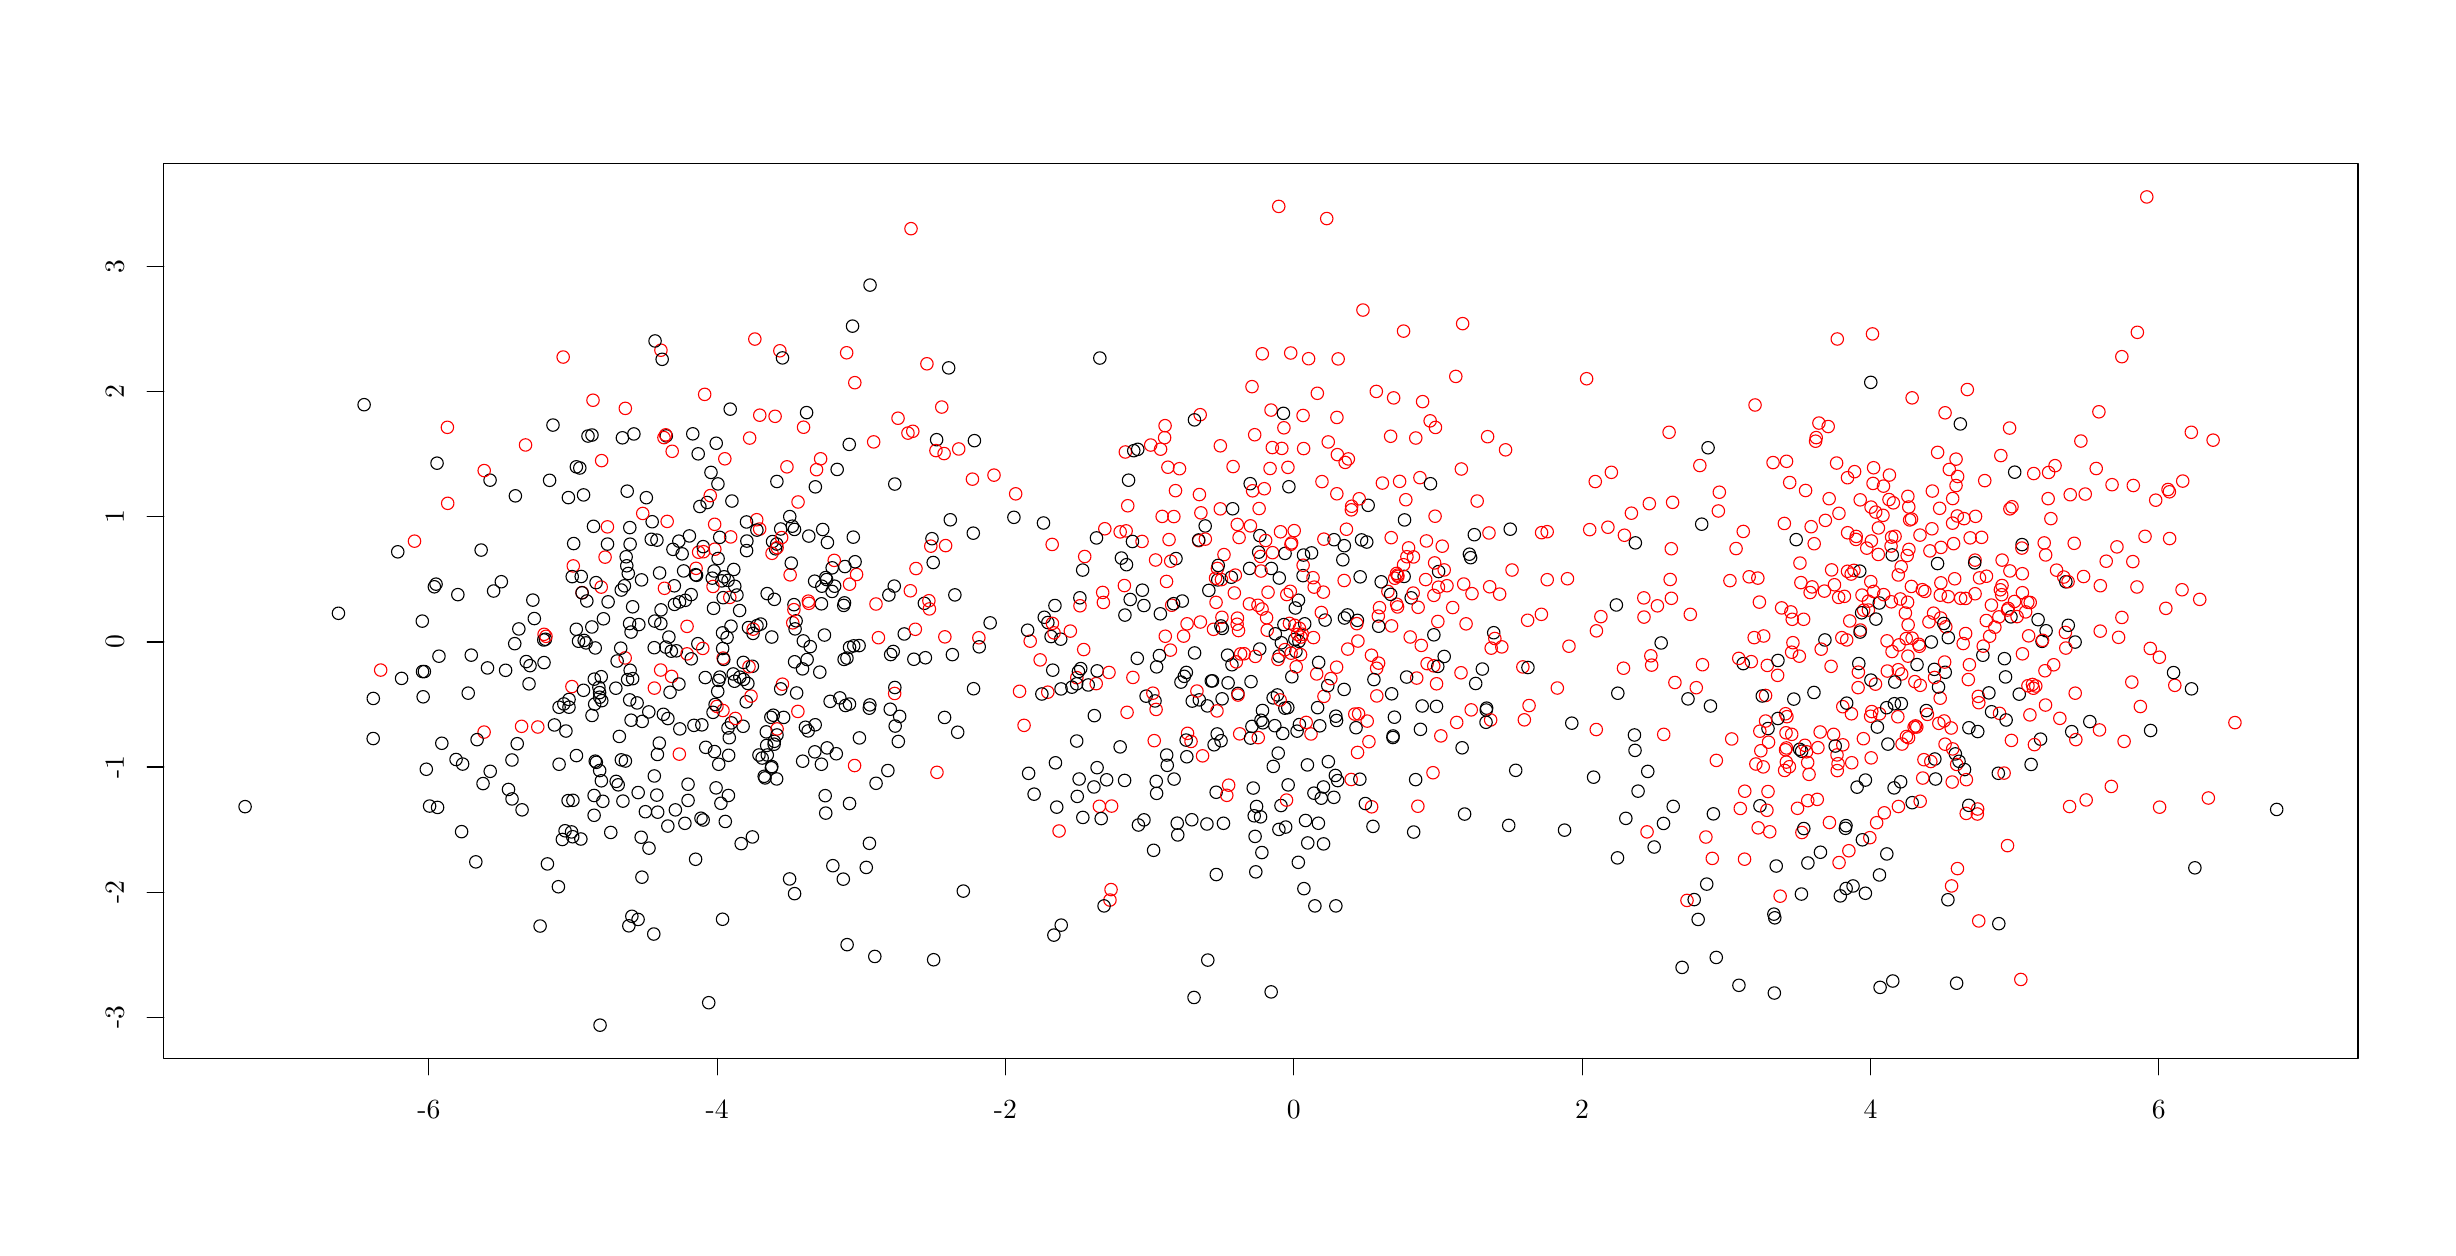
\begin{tikzpicture}[x=1pt,y=1pt]
\definecolor{fillColor}{RGB}{255,255,255}
\path[use as bounding box,fill=fillColor,fill opacity=0.00] (0,0) rectangle (867.24,433.62);
\begin{scope}
\path[clip] ( 49.20, 61.20) rectangle (842.04,384.42);
\definecolor{drawColor}{RGB}{0,0,0}

\path[draw=drawColor,line width= 0.4pt,line join=round,line cap=round] (468.82,219.55) circle (  2.25);
\definecolor{drawColor}{RGB}{255,0,0}

\path[draw=drawColor,line width= 0.4pt,line join=round,line cap=round] (381.96,242.52) circle (  2.25);

\path[draw=drawColor,line width= 0.4pt,line join=round,line cap=round] (654.50,258.12) circle (  2.25);
\definecolor{drawColor}{RGB}{0,0,0}

\path[draw=drawColor,line width= 0.4pt,line join=round,line cap=round] (591.10,146.06) circle (  2.25);
\definecolor{drawColor}{RGB}{255,0,0}

\path[draw=drawColor,line width= 0.4pt,line join=round,line cap=round] (556.40,234.49) circle (  2.25);
\definecolor{drawColor}{RGB}{0,0,0}

\path[draw=drawColor,line width= 0.4pt,line join=round,line cap=round] (460.86,235.60) circle (  2.25);
\definecolor{drawColor}{RGB}{255,0,0}

\path[draw=drawColor,line width= 0.4pt,line join=round,line cap=round] (666.62,322.95) circle (  2.25);
\definecolor{drawColor}{RGB}{0,0,0}

\path[draw=drawColor,line width= 0.4pt,line join=round,line cap=round] (142.68,200.95) circle (  2.25);

\path[draw=drawColor,line width= 0.4pt,line join=round,line cap=round] (625.95,152.44) circle (  2.25);
\definecolor{drawColor}{RGB}{255,0,0}

\path[draw=drawColor,line width= 0.4pt,line join=round,line cap=round] (204.28,298.99) circle (  2.25);
\definecolor{drawColor}{RGB}{0,0,0}

\path[draw=drawColor,line width= 0.4pt,line join=round,line cap=round] (327.37, 96.81) circle (  2.25);

\path[draw=drawColor,line width= 0.4pt,line join=round,line cap=round] (647.82,135.66) circle (  2.25);

\path[draw=drawColor,line width= 0.4pt,line join=round,line cap=round] (213.80,177.51) circle (  2.25);

\path[draw=drawColor,line width= 0.4pt,line join=round,line cap=round] (282.78,209.96) circle (  2.25);

\path[draw=drawColor,line width= 0.4pt,line join=round,line cap=round] (458.28,208.24) circle (  2.25);
\definecolor{drawColor}{RGB}{255,0,0}

\path[draw=drawColor,line width= 0.4pt,line join=round,line cap=round] (635.51,173.34) circle (  2.25);
\definecolor{drawColor}{RGB}{0,0,0}

\path[draw=drawColor,line width= 0.4pt,line join=round,line cap=round] (602.19,118.55) circle (  2.25);

\path[draw=drawColor,line width= 0.4pt,line join=round,line cap=round] (249.35,193.78) circle (  2.25);
\definecolor{drawColor}{RGB}{255,0,0}

\path[draw=drawColor,line width= 0.4pt,line join=round,line cap=round] (704.61,151.28) circle (  2.25);

\path[draw=drawColor,line width= 0.4pt,line join=round,line cap=round] (437.53,215.77) circle (  2.25);

\path[draw=drawColor,line width= 0.4pt,line join=round,line cap=round] (657.30,212.38) circle (  2.25);
\definecolor{drawColor}{RGB}{0,0,0}

\path[draw=drawColor,line width= 0.4pt,line join=round,line cap=round] (745.15,182.87) circle (  2.25);

\path[draw=drawColor,line width= 0.4pt,line join=round,line cap=round] (664.06,161.74) circle (  2.25);

\path[draw=drawColor,line width= 0.4pt,line join=round,line cap=round] (407.36,190.33) circle (  2.25);

\path[draw=drawColor,line width= 0.4pt,line join=round,line cap=round] (334.14,207.07) circle (  2.25);

\path[draw=drawColor,line width= 0.4pt,line join=round,line cap=round] (674.53,189.32) circle (  2.25);

\path[draw=drawColor,line width= 0.4pt,line join=round,line cap=round] (523.24,196.64) circle (  2.25);

\path[draw=drawColor,line width= 0.4pt,line join=round,line cap=round] (196.53,143.00) circle (  2.25);

\path[draw=drawColor,line width= 0.4pt,line join=round,line cap=round] (475.23,241.33) circle (  2.25);

\path[draw=drawColor,line width= 0.4pt,line join=round,line cap=round] (603.62,111.38) circle (  2.25);

\path[draw=drawColor,line width= 0.4pt,line join=round,line cap=round] (783.11,130.03) circle (  2.25);
\definecolor{drawColor}{RGB}{255,0,0}

\path[draw=drawColor,line width= 0.4pt,line join=round,line cap=round] (683.87,195.98) circle (  2.25);
\definecolor{drawColor}{RGB}{0,0,0}

\path[draw=drawColor,line width= 0.4pt,line join=round,line cap=round] (194.50,179.46) circle (  2.25);
\definecolor{drawColor}{RGB}{255,0,0}

\path[draw=drawColor,line width= 0.4pt,line join=round,line cap=round] (215.91,205.87) circle (  2.25);
\definecolor{drawColor}{RGB}{0,0,0}

\path[draw=drawColor,line width= 0.4pt,line join=round,line cap=round] (404.14,192.06) circle (  2.25);

\path[draw=drawColor,line width= 0.4pt,line join=round,line cap=round] (144.04,165.65) circle (  2.25);
\definecolor{drawColor}{RGB}{255,0,0}

\path[draw=drawColor,line width= 0.4pt,line join=round,line cap=round] (658.08,136.20) circle (  2.25);

\path[draw=drawColor,line width= 0.4pt,line join=round,line cap=round] (692.84,174.71) circle (  2.25);

\path[draw=drawColor,line width= 0.4pt,line join=round,line cap=round] (388.45,229.54) circle (  2.25);
\definecolor{drawColor}{RGB}{0,0,0}

\path[draw=drawColor,line width= 0.4pt,line join=round,line cap=round] (453.01,211.35) circle (  2.25);
\definecolor{drawColor}{RGB}{255,0,0}

\path[draw=drawColor,line width= 0.4pt,line join=round,line cap=round] (660.74,249.78) circle (  2.25);

\path[draw=drawColor,line width= 0.4pt,line join=round,line cap=round] (320.99,238.18) circle (  2.25);

\path[draw=drawColor,line width= 0.4pt,line join=round,line cap=round] (733.13,237.60) circle (  2.25);

\path[draw=drawColor,line width= 0.4pt,line join=round,line cap=round] (207.40,277.17) circle (  2.25);

\path[draw=drawColor,line width= 0.4pt,line join=round,line cap=round] (394.77,251.42) circle (  2.25);
\definecolor{drawColor}{RGB}{0,0,0}

\path[draw=drawColor,line width= 0.4pt,line join=round,line cap=round] (253.08,233.90) circle (  2.25);

\path[draw=drawColor,line width= 0.4pt,line join=round,line cap=round] (194.18,143.42) circle (  2.25);

\path[draw=drawColor,line width= 0.4pt,line join=round,line cap=round] (726.46,219.70) circle (  2.25);

\path[draw=drawColor,line width= 0.4pt,line join=round,line cap=round] (241.69,235.73) circle (  2.25);
\definecolor{drawColor}{RGB}{255,0,0}

\path[draw=drawColor,line width= 0.4pt,line join=round,line cap=round] (518.91,232.58) circle (  2.25);
\definecolor{drawColor}{RGB}{0,0,0}

\path[draw=drawColor,line width= 0.4pt,line join=round,line cap=round] (452.26,234.75) circle (  2.25);
\definecolor{drawColor}{RGB}{255,0,0}

\path[draw=drawColor,line width= 0.4pt,line join=round,line cap=round] (197.15,239.12) circle (  2.25);

\path[draw=drawColor,line width= 0.4pt,line join=round,line cap=round] (675.93,201.62) circle (  2.25);
\definecolor{drawColor}{RGB}{0,0,0}

\path[draw=drawColor,line width= 0.4pt,line join=round,line cap=round] (250.50,153.35) circle (  2.25);

\path[draw=drawColor,line width= 0.4pt,line join=round,line cap=round] (430.04,234.07) circle (  2.25);
\definecolor{drawColor}{RGB}{255,0,0}

\path[draw=drawColor,line width= 0.4pt,line join=round,line cap=round] (455.39,274.73) circle (  2.25);
\definecolor{drawColor}{RGB}{0,0,0}

\path[draw=drawColor,line width= 0.4pt,line join=round,line cap=round] (481.99,248.52) circle (  2.25);

\path[draw=drawColor,line width= 0.4pt,line join=round,line cap=round] (450.09,166.68) circle (  2.25);

\path[draw=drawColor,line width= 0.4pt,line join=round,line cap=round] (394.76,173.73) circle (  2.25);

\path[draw=drawColor,line width= 0.4pt,line join=round,line cap=round] (716.66,220.72) circle (  2.25);
\definecolor{drawColor}{RGB}{255,0,0}

\path[draw=drawColor,line width= 0.4pt,line join=round,line cap=round] (568.48,220.80) circle (  2.25);
\definecolor{drawColor}{RGB}{0,0,0}

\path[draw=drawColor,line width= 0.4pt,line join=round,line cap=round] (452.18,206.56) circle (  2.25);
\definecolor{drawColor}{RGB}{255,0,0}

\path[draw=drawColor,line width= 0.4pt,line join=round,line cap=round] (773.41,266.73) circle (  2.25);
\definecolor{drawColor}{RGB}{0,0,0}

\path[draw=drawColor,line width= 0.4pt,line join=round,line cap=round] (295.02,205.33) circle (  2.25);
\definecolor{drawColor}{RGB}{255,0,0}

\path[draw=drawColor,line width= 0.4pt,line join=round,line cap=round] (460.88,239.36) circle (  2.25);
\definecolor{drawColor}{RGB}{0,0,0}

\path[draw=drawColor,line width= 0.4pt,line join=round,line cap=round] (203.86,217.06) circle (  2.25);

\path[draw=drawColor,line width= 0.4pt,line join=round,line cap=round] (304.17,138.89) circle (  2.25);

\path[draw=drawColor,line width= 0.4pt,line join=round,line cap=round] (295.16,225.77) circle (  2.25);
\definecolor{drawColor}{RGB}{255,0,0}

\path[draw=drawColor,line width= 0.4pt,line join=round,line cap=round] (784.87,227.03) circle (  2.25);

\path[draw=drawColor,line width= 0.4pt,line join=round,line cap=round] (254.03,249.60) circle (  2.25);

\path[draw=drawColor,line width= 0.4pt,line join=round,line cap=round] (696.81,277.71) circle (  2.25);

\path[draw=drawColor,line width= 0.4pt,line join=round,line cap=round] (748.43,294.81) circle (  2.25);
\definecolor{drawColor}{RGB}{0,0,0}

\path[draw=drawColor,line width= 0.4pt,line join=round,line cap=round] (253.30,170.69) circle (  2.25);

\path[draw=drawColor,line width= 0.4pt,line join=round,line cap=round] (701.45,180.64) circle (  2.25);

\path[draw=drawColor,line width= 0.4pt,line join=round,line cap=round] (720.67,246.82) circle (  2.25);

\path[draw=drawColor,line width= 0.4pt,line join=round,line cap=round] (225.66,255.09) circle (  2.25);
\definecolor{drawColor}{RGB}{255,0,0}

\path[draw=drawColor,line width= 0.4pt,line join=round,line cap=round] (186.60,214.41) circle (  2.25);

\path[draw=drawColor,line width= 0.4pt,line join=round,line cap=round] (701.91,249.26) circle (  2.25);

\path[draw=drawColor,line width= 0.4pt,line join=round,line cap=round] (720.76,236.30) circle (  2.25);
\definecolor{drawColor}{RGB}{0,0,0}

\path[draw=drawColor,line width= 0.4pt,line join=round,line cap=round] (281.65,205.30) circle (  2.25);

\path[draw=drawColor,line width= 0.4pt,line join=round,line cap=round] (414.94,241.78) circle (  2.25);
\definecolor{drawColor}{RGB}{255,0,0}

\path[draw=drawColor,line width= 0.4pt,line join=round,line cap=round] (690.59,182.23) circle (  2.25);
\definecolor{drawColor}{RGB}{0,0,0}

\path[draw=drawColor,line width= 0.4pt,line join=round,line cap=round] (214.30,209.40) circle (  2.25);

\path[draw=drawColor,line width= 0.4pt,line join=round,line cap=round] (295.31,238.90) circle (  2.25);

\path[draw=drawColor,line width= 0.4pt,line join=round,line cap=round] (426.81,230.28) circle (  2.25);
\definecolor{drawColor}{RGB}{255,0,0}

\path[draw=drawColor,line width= 0.4pt,line join=round,line cap=round] (270.08,293.18) circle (  2.25);

\path[draw=drawColor,line width= 0.4pt,line join=round,line cap=round] (387.25,152.27) circle (  2.25);

\path[draw=drawColor,line width= 0.4pt,line join=round,line cap=round] (423.16,248.23) circle (  2.25);
\definecolor{drawColor}{RGB}{0,0,0}

\path[draw=drawColor,line width= 0.4pt,line join=round,line cap=round] (311.84,207.09) circle (  2.25);

\path[draw=drawColor,line width= 0.4pt,line join=round,line cap=round] (252.72,213.27) circle (  2.25);
\definecolor{drawColor}{RGB}{255,0,0}

\path[draw=drawColor,line width= 0.4pt,line join=round,line cap=round] (705.29,234.79) circle (  2.25);
\definecolor{drawColor}{RGB}{0,0,0}

\path[draw=drawColor,line width= 0.4pt,line join=round,line cap=round] (449.33, 85.20) circle (  2.25);

\path[draw=drawColor,line width= 0.4pt,line join=round,line cap=round] (257.26,223.00) circle (  2.25);

\path[draw=drawColor,line width= 0.4pt,line join=round,line cap=round] (431.60,191.09) circle (  2.25);
\definecolor{drawColor}{RGB}{255,0,0}

\path[draw=drawColor,line width= 0.4pt,line join=round,line cap=round] (665.14,223.18) circle (  2.25);

\path[draw=drawColor,line width= 0.4pt,line join=round,line cap=round] (492.50,285.98) circle (  2.25);

\path[draw=drawColor,line width= 0.4pt,line join=round,line cap=round] (253.71,227.75) circle (  2.25);

\path[draw=drawColor,line width= 0.4pt,line join=round,line cap=round] (666.21,248.13) circle (  2.25);
\definecolor{drawColor}{RGB}{0,0,0}

\path[draw=drawColor,line width= 0.4pt,line join=round,line cap=round] (397.80,270.10) circle (  2.25);

\path[draw=drawColor,line width= 0.4pt,line join=round,line cap=round] (371.39,167.97) circle (  2.25);
\definecolor{drawColor}{RGB}{255,0,0}

\path[draw=drawColor,line width= 0.4pt,line join=round,line cap=round] (285.05,273.90) circle (  2.25);

\path[draw=drawColor,line width= 0.4pt,line join=round,line cap=round] (723.50,185.29) circle (  2.25);

\path[draw=drawColor,line width= 0.4pt,line join=round,line cap=round] (743.49,265.09) circle (  2.25);

\path[draw=drawColor,line width= 0.4pt,line join=round,line cap=round] (412.93,208.70) circle (  2.25);

\path[draw=drawColor,line width= 0.4pt,line join=round,line cap=round] (760.86,268.18) circle (  2.25);

\path[draw=drawColor,line width= 0.4pt,line join=round,line cap=round] (449.84,243.91) circle (  2.25);
\definecolor{drawColor}{RGB}{0,0,0}

\path[draw=drawColor,line width= 0.4pt,line join=round,line cap=round] (316.75,214.53) circle (  2.25);

\path[draw=drawColor,line width= 0.4pt,line join=round,line cap=round] (296.98,209.69) circle (  2.25);

\path[draw=drawColor,line width= 0.4pt,line join=round,line cap=round] (183.07,220.10) circle (  2.25);
\definecolor{drawColor}{RGB}{255,0,0}

\path[draw=drawColor,line width= 0.4pt,line join=round,line cap=round] (586.82,203.28) circle (  2.25);
\definecolor{drawColor}{RGB}{0,0,0}

\path[draw=drawColor,line width= 0.4pt,line join=round,line cap=round] (214.49,230.41) circle (  2.25);

\path[draw=drawColor,line width= 0.4pt,line join=round,line cap=round] (198.24,216.23) circle (  2.25);

\path[draw=drawColor,line width= 0.4pt,line join=round,line cap=round] (639.04,248.62) circle (  2.25);

\path[draw=drawColor,line width= 0.4pt,line join=round,line cap=round] (336.06,179.02) circle (  2.25);

\path[draw=drawColor,line width= 0.4pt,line join=round,line cap=round] (697.02, 88.34) circle (  2.25);
\definecolor{drawColor}{RGB}{255,0,0}

\path[draw=drawColor,line width= 0.4pt,line join=round,line cap=round] (635.21,185.71) circle (  2.25);

\path[draw=drawColor,line width= 0.4pt,line join=round,line cap=round] (625.31,144.47) circle (  2.25);

\path[draw=drawColor,line width= 0.4pt,line join=round,line cap=round] (659.01,185.69) circle (  2.25);
\definecolor{drawColor}{RGB}{0,0,0}

\path[draw=drawColor,line width= 0.4pt,line join=round,line cap=round] (398.39,226.99) circle (  2.25);
\definecolor{drawColor}{RGB}{255,0,0}

\path[draw=drawColor,line width= 0.4pt,line join=round,line cap=round] (396.63,280.29) circle (  2.25);

\path[draw=drawColor,line width= 0.4pt,line join=round,line cap=round] (664.55,245.55) circle (  2.25);
\definecolor{drawColor}{RGB}{0,0,0}

\path[draw=drawColor,line width= 0.4pt,line join=round,line cap=round] (443.20,148.83) circle (  2.25);
\definecolor{drawColor}{RGB}{255,0,0}

\path[draw=drawColor,line width= 0.4pt,line join=round,line cap=round] (775.86,195.97) circle (  2.25);

\path[draw=drawColor,line width= 0.4pt,line join=round,line cap=round] (503.57,210.40) circle (  2.25);
\definecolor{drawColor}{RGB}{0,0,0}

\path[draw=drawColor,line width= 0.4pt,line join=round,line cap=round] (775.41,200.57) circle (  2.25);
\definecolor{drawColor}{RGB}{255,0,0}

\path[draw=drawColor,line width= 0.4pt,line join=round,line cap=round] (469.95,283.92) circle (  2.25);

\path[draw=drawColor,line width= 0.4pt,line join=round,line cap=round] (391.68,152.34) circle (  2.25);
\definecolor{drawColor}{RGB}{0,0,0}

\path[draw=drawColor,line width= 0.4pt,line join=round,line cap=round] (577.49,147.90) circle (  2.25);
\definecolor{drawColor}{RGB}{255,0,0}

\path[draw=drawColor,line width= 0.4pt,line join=round,line cap=round] (717.94,226.28) circle (  2.25);

\path[draw=drawColor,line width= 0.4pt,line join=round,line cap=round] (566.86,215.66) circle (  2.25);
\definecolor{drawColor}{RGB}{0,0,0}

\path[draw=drawColor,line width= 0.4pt,line join=round,line cap=round] (112.30,222.01) circle (  2.25);
\definecolor{drawColor}{RGB}{255,0,0}

\path[draw=drawColor,line width= 0.4pt,line join=round,line cap=round] (487.50,192.14) circle (  2.25);
\definecolor{drawColor}{RGB}{0,0,0}

\path[draw=drawColor,line width= 0.4pt,line join=round,line cap=round] (217.58,252.97) circle (  2.25);

\path[draw=drawColor,line width= 0.4pt,line join=round,line cap=round] (275.32,126.01) circle (  2.25);

\path[draw=drawColor,line width= 0.4pt,line join=round,line cap=round] (781.90,194.70) circle (  2.25);
\definecolor{drawColor}{RGB}{255,0,0}

\path[draw=drawColor,line width= 0.4pt,line join=round,line cap=round] (409.37,281.31) circle (  2.25);

\path[draw=drawColor,line width= 0.4pt,line join=round,line cap=round] (715.42,223.18) circle (  2.25);

\path[draw=drawColor,line width= 0.4pt,line join=round,line cap=round] (644.08,229.51) circle (  2.25);
\definecolor{drawColor}{RGB}{0,0,0}

\path[draw=drawColor,line width= 0.4pt,line join=round,line cap=round] (189.82,290.02) circle (  2.25);
\definecolor{drawColor}{RGB}{255,0,0}

\path[draw=drawColor,line width= 0.4pt,line join=round,line cap=round] (306.54,225.36) circle (  2.25);
\definecolor{drawColor}{RGB}{0,0,0}

\path[draw=drawColor,line width= 0.4pt,line join=round,line cap=round] (767.12,179.65) circle (  2.25);
\definecolor{drawColor}{RGB}{255,0,0}

\path[draw=drawColor,line width= 0.4pt,line join=round,line cap=round] (528.29,231.59) circle (  2.25);
\definecolor{drawColor}{RGB}{0,0,0}

\path[draw=drawColor,line width= 0.4pt,line join=round,line cap=round] (210.70,142.81) circle (  2.25);
\definecolor{drawColor}{RGB}{255,0,0}

\path[draw=drawColor,line width= 0.4pt,line join=round,line cap=round] (263.45,255.81) circle (  2.25);
\definecolor{drawColor}{RGB}{0,0,0}

\path[draw=drawColor,line width= 0.4pt,line join=round,line cap=round] (304.38,340.60) circle (  2.25);
\definecolor{drawColor}{RGB}{255,0,0}

\path[draw=drawColor,line width= 0.4pt,line join=round,line cap=round] (650.96,263.41) circle (  2.25);

\path[draw=drawColor,line width= 0.4pt,line join=round,line cap=round] (324.94,312.16) circle (  2.25);
\definecolor{drawColor}{RGB}{0,0,0}

\path[draw=drawColor,line width= 0.4pt,line join=round,line cap=round] (451.88,171.48) circle (  2.25);
\definecolor{drawColor}{RGB}{255,0,0}

\path[draw=drawColor,line width= 0.4pt,line join=round,line cap=round] (478.24,161.95) circle (  2.25);

\path[draw=drawColor,line width= 0.4pt,line join=round,line cap=round] (509.09,196.53) circle (  2.25);

\path[draw=drawColor,line width= 0.4pt,line join=round,line cap=round] (464.46,234.86) circle (  2.25);
\definecolor{drawColor}{RGB}{0,0,0}

\path[draw=drawColor,line width= 0.4pt,line join=round,line cap=round] (216.64,266.13) circle (  2.25);

\path[draw=drawColor,line width= 0.4pt,line join=round,line cap=round] (295.50,188.69) circle (  2.25);
\definecolor{drawColor}{RGB}{255,0,0}

\path[draw=drawColor,line width= 0.4pt,line join=round,line cap=round] (448.93,274.33) circle (  2.25);
\definecolor{drawColor}{RGB}{0,0,0}

\path[draw=drawColor,line width= 0.4pt,line join=round,line cap=round] (452.88,152.54) circle (  2.25);
\definecolor{drawColor}{RGB}{255,0,0}

\path[draw=drawColor,line width= 0.4pt,line join=round,line cap=round] (451.79,205.34) circle (  2.25);
\definecolor{drawColor}{RGB}{0,0,0}

\path[draw=drawColor,line width= 0.4pt,line join=round,line cap=round] (469.99,168.38) circle (  2.25);
\definecolor{drawColor}{RGB}{255,0,0}

\path[draw=drawColor,line width= 0.4pt,line join=round,line cap=round] (672.58,263.11) circle (  2.25);
\definecolor{drawColor}{RGB}{0,0,0}

\path[draw=drawColor,line width= 0.4pt,line join=round,line cap=round] (224.44,186.37) circle (  2.25);

\path[draw=drawColor,line width= 0.4pt,line join=round,line cap=round] (204.89,189.19) circle (  2.25);

\path[draw=drawColor,line width= 0.4pt,line join=round,line cap=round] (269.43,185.17) circle (  2.25);

\path[draw=drawColor,line width= 0.4pt,line join=round,line cap=round] (718.01,273.00) circle (  2.25);
\definecolor{drawColor}{RGB}{255,0,0}

\path[draw=drawColor,line width= 0.4pt,line join=round,line cap=round] (331.70,246.46) circle (  2.25);
\definecolor{drawColor}{RGB}{0,0,0}

\path[draw=drawColor,line width= 0.4pt,line join=round,line cap=round] (690.13,239.98) circle (  2.25);
\definecolor{drawColor}{RGB}{255,0,0}

\path[draw=drawColor,line width= 0.4pt,line join=round,line cap=round] (184.33,180.91) circle (  2.25);
\definecolor{drawColor}{RGB}{0,0,0}

\path[draw=drawColor,line width= 0.4pt,line join=round,line cap=round] (147.56,232.54) circle (  2.25);
\definecolor{drawColor}{RGB}{255,0,0}

\path[draw=drawColor,line width= 0.4pt,line join=round,line cap=round] (457.65,251.87) circle (  2.25);
\definecolor{drawColor}{RGB}{0,0,0}

\path[draw=drawColor,line width= 0.4pt,line join=round,line cap=round] (475.76,246.42) circle (  2.25);
\definecolor{drawColor}{RGB}{255,0,0}

\path[draw=drawColor,line width= 0.4pt,line join=round,line cap=round] (209.49,253.23) circle (  2.25);
\definecolor{drawColor}{RGB}{0,0,0}

\path[draw=drawColor,line width= 0.4pt,line join=round,line cap=round] (610.16, 97.64) circle (  2.25);

\path[draw=drawColor,line width= 0.4pt,line join=round,line cap=round] (426.43, 96.69) circle (  2.25);

\path[draw=drawColor,line width= 0.4pt,line join=round,line cap=round] (221.68,141.07) circle (  2.25);
\definecolor{drawColor}{RGB}{255,0,0}

\path[draw=drawColor,line width= 0.4pt,line join=round,line cap=round] (251.31,205.81) circle (  2.25);

\path[draw=drawColor,line width= 0.4pt,line join=round,line cap=round] (241.53,238.25) circle (  2.25);

\path[draw=drawColor,line width= 0.4pt,line join=round,line cap=round] (455.93,218.36) circle (  2.25);
\definecolor{drawColor}{RGB}{0,0,0}

\path[draw=drawColor,line width= 0.4pt,line join=round,line cap=round] (146.95,231.58) circle (  2.25);
\definecolor{drawColor}{RGB}{255,0,0}

\path[draw=drawColor,line width= 0.4pt,line join=round,line cap=round] (667.78,258.57) circle (  2.25);

\path[draw=drawColor,line width= 0.4pt,line join=round,line cap=round] (264.54,293.59) circle (  2.25);

\path[draw=drawColor,line width= 0.4pt,line join=round,line cap=round] (665.66,140.92) circle (  2.25);

\path[draw=drawColor,line width= 0.4pt,line join=round,line cap=round] (437.96,178.44) circle (  2.25);
\definecolor{drawColor}{RGB}{0,0,0}

\path[draw=drawColor,line width= 0.4pt,line join=round,line cap=round] (267.04,174.25) circle (  2.25);
\definecolor{drawColor}{RGB}{255,0,0}

\path[draw=drawColor,line width= 0.4pt,line join=round,line cap=round] (695.56,254.58) circle (  2.25);

\path[draw=drawColor,line width= 0.4pt,line join=round,line cap=round] (637.43,178.26) circle (  2.25);
\definecolor{drawColor}{RGB}{0,0,0}

\path[draw=drawColor,line width= 0.4pt,line join=round,line cap=round] (459.36,211.88) circle (  2.25);
\definecolor{drawColor}{RGB}{255,0,0}

\path[draw=drawColor,line width= 0.4pt,line join=round,line cap=round] (485.64,152.07) circle (  2.25);

\path[draw=drawColor,line width= 0.4pt,line join=round,line cap=round] (610.19,168.84) circle (  2.25);

\path[draw=drawColor,line width= 0.4pt,line join=round,line cap=round] (501.58,285.34) circle (  2.25);
\definecolor{drawColor}{RGB}{0,0,0}

\path[draw=drawColor,line width= 0.4pt,line join=round,line cap=round] (248.03,237.29) circle (  2.25);
\definecolor{drawColor}{RGB}{255,0,0}

\path[draw=drawColor,line width= 0.4pt,line join=round,line cap=round] (314.50,292.49) circle (  2.25);
\definecolor{drawColor}{RGB}{0,0,0}

\path[draw=drawColor,line width= 0.4pt,line join=round,line cap=round] (519.23,149.46) circle (  2.25);

\path[draw=drawColor,line width= 0.4pt,line join=round,line cap=round] (277.87,193.21) circle (  2.25);

\path[draw=drawColor,line width= 0.4pt,line join=round,line cap=round] (673.94, 89.13) circle (  2.25);
\definecolor{drawColor}{RGB}{255,0,0}

\path[draw=drawColor,line width= 0.4pt,line join=round,line cap=round] (444.56,224.90) circle (  2.25);
\definecolor{drawColor}{RGB}{0,0,0}

\path[draw=drawColor,line width= 0.4pt,line join=round,line cap=round] (481.38,162.05) circle (  2.25);
\definecolor{drawColor}{RGB}{255,0,0}

\path[draw=drawColor,line width= 0.4pt,line join=round,line cap=round] (411.00,289.80) circle (  2.25);
\definecolor{drawColor}{RGB}{0,0,0}

\path[draw=drawColor,line width= 0.4pt,line join=round,line cap=round] (535.72,252.40) circle (  2.25);

\path[draw=drawColor,line width= 0.4pt,line join=round,line cap=round] (580.81,172.47) circle (  2.25);

\path[draw=drawColor,line width= 0.4pt,line join=round,line cap=round] (292.18,171.25) circle (  2.25);
\definecolor{drawColor}{RGB}{255,0,0}

\path[draw=drawColor,line width= 0.4pt,line join=round,line cap=round] (409.94,257.01) circle (  2.25);
\definecolor{drawColor}{RGB}{0,0,0}

\path[draw=drawColor,line width= 0.4pt,line join=round,line cap=round] (401.13,281.25) circle (  2.25);

\path[draw=drawColor,line width= 0.4pt,line join=round,line cap=round] (268.88,213.43) circle (  2.25);
\definecolor{drawColor}{RGB}{255,0,0}

\path[draw=drawColor,line width= 0.4pt,line join=round,line cap=round] (431.36,234.17) circle (  2.25);
\definecolor{drawColor}{RGB}{0,0,0}

\path[draw=drawColor,line width= 0.4pt,line join=round,line cap=round] (455.74,267.73) circle (  2.25);

\path[draw=drawColor,line width= 0.4pt,line join=round,line cap=round] (245.52,262.04) circle (  2.25);

\path[draw=drawColor,line width= 0.4pt,line join=round,line cap=round] (673.75,243.10) circle (  2.25);

\path[draw=drawColor,line width= 0.4pt,line join=round,line cap=round] (264.85,218.12) circle (  2.25);

\path[draw=drawColor,line width= 0.4pt,line join=round,line cap=round] (338.09,121.62) circle (  2.25);

\path[draw=drawColor,line width= 0.4pt,line join=round,line cap=round] (261.87,202.86) circle (  2.25);

\path[draw=drawColor,line width= 0.4pt,line join=round,line cap=round] (452.13,143.91) circle (  2.25);
\definecolor{drawColor}{RGB}{255,0,0}

\path[draw=drawColor,line width= 0.4pt,line join=round,line cap=round] (635.56,276.92) circle (  2.25);
\definecolor{drawColor}{RGB}{0,0,0}

\path[draw=drawColor,line width= 0.4pt,line join=round,line cap=round] (268.74,166.17) circle (  2.25);

\path[draw=drawColor,line width= 0.4pt,line join=round,line cap=round] (191.78,123.19) circle (  2.25);

\path[draw=drawColor,line width= 0.4pt,line join=round,line cap=round] (518.33,173.40) circle (  2.25);

\path[draw=drawColor,line width= 0.4pt,line join=round,line cap=round] (229.71,185.50) circle (  2.25);
\definecolor{drawColor}{RGB}{255,0,0}

\path[draw=drawColor,line width= 0.4pt,line join=round,line cap=round] (670.41,257.40) circle (  2.25);

\path[draw=drawColor,line width= 0.4pt,line join=round,line cap=round] (505.68,203.82) circle (  2.25);

\path[draw=drawColor,line width= 0.4pt,line join=round,line cap=round] (402.67,247.97) circle (  2.25);

\path[draw=drawColor,line width= 0.4pt,line join=round,line cap=round] (437.04,218.05) circle (  2.25);

\path[draw=drawColor,line width= 0.4pt,line join=round,line cap=round] (473.06,265.19) circle (  2.25);
\definecolor{drawColor}{RGB}{0,0,0}

\path[draw=drawColor,line width= 0.4pt,line join=round,line cap=round] (443.78,128.57) circle (  2.25);

\path[draw=drawColor,line width= 0.4pt,line join=round,line cap=round] (472.05,248.59) circle (  2.25);

\path[draw=drawColor,line width= 0.4pt,line join=round,line cap=round] (251.13,209.28) circle (  2.25);

\path[draw=drawColor,line width= 0.4pt,line join=round,line cap=round] (727.34,176.53) circle (  2.25);
\definecolor{drawColor}{RGB}{255,0,0}

\path[draw=drawColor,line width= 0.4pt,line join=round,line cap=round] (628.60,203.17) circle (  2.25);

\path[draw=drawColor,line width= 0.4pt,line join=round,line cap=round] (379.11,198.75) circle (  2.25);

\path[draw=drawColor,line width= 0.4pt,line join=round,line cap=round] (464.62,213.22) circle (  2.25);

\path[draw=drawColor,line width= 0.4pt,line join=round,line cap=round] (449.74,281.89) circle (  2.25);
\definecolor{drawColor}{RGB}{0,0,0}

\path[draw=drawColor,line width= 0.4pt,line join=round,line cap=round] (186.49,212.36) circle (  2.25);
\definecolor{drawColor}{RGB}{255,0,0}

\path[draw=drawColor,line width= 0.4pt,line join=round,line cap=round] (730.09,263.43) circle (  2.25);
\definecolor{drawColor}{RGB}{0,0,0}

\path[draw=drawColor,line width= 0.4pt,line join=round,line cap=round] (686.06,186.85) circle (  2.25);

\path[draw=drawColor,line width= 0.4pt,line join=round,line cap=round] (231.34,183.97) circle (  2.25);
\definecolor{drawColor}{RGB}{255,0,0}

\path[draw=drawColor,line width= 0.4pt,line join=round,line cap=round] (677.17,200.08) circle (  2.25);
\definecolor{drawColor}{RGB}{0,0,0}

\path[draw=drawColor,line width= 0.4pt,line join=round,line cap=round] (475.69,194.49) circle (  2.25);
\definecolor{drawColor}{RGB}{255,0,0}

\path[draw=drawColor,line width= 0.4pt,line join=round,line cap=round] (725.62,195.73) circle (  2.25);

\path[draw=drawColor,line width= 0.4pt,line join=round,line cap=round] (248.24,254.16) circle (  2.25);
\definecolor{drawColor}{RGB}{0,0,0}

\path[draw=drawColor,line width= 0.4pt,line join=round,line cap=round] (296.04,205.82) circle (  2.25);
\definecolor{drawColor}{RGB}{255,0,0}

\path[draw=drawColor,line width= 0.4pt,line join=round,line cap=round] (305.70,283.94) circle (  2.25);
\definecolor{drawColor}{RGB}{0,0,0}

\path[draw=drawColor,line width= 0.4pt,line join=round,line cap=round] (599.95,191.07) circle (  2.25);
\definecolor{drawColor}{RGB}{255,0,0}

\path[draw=drawColor,line width= 0.4pt,line join=round,line cap=round] (416.21,274.25) circle (  2.25);

\path[draw=drawColor,line width= 0.4pt,line join=round,line cap=round] (396.93,251.78) circle (  2.25);
\definecolor{drawColor}{RGB}{0,0,0}

\path[draw=drawColor,line width= 0.4pt,line join=round,line cap=round] (696.56,171.20) circle (  2.25);
\definecolor{drawColor}{RGB}{255,0,0}

\path[draw=drawColor,line width= 0.4pt,line join=round,line cap=round] (651.65,202.84) circle (  2.25);

\path[draw=drawColor,line width= 0.4pt,line join=round,line cap=round] (532.67,209.86) circle (  2.25);
\definecolor{drawColor}{RGB}{0,0,0}

\path[draw=drawColor,line width= 0.4pt,line join=round,line cap=round] (235.65,180.23) circle (  2.25);
\definecolor{drawColor}{RGB}{255,0,0}

\path[draw=drawColor,line width= 0.4pt,line join=round,line cap=round] (666.10,260.38) circle (  2.25);

\path[draw=drawColor,line width= 0.4pt,line join=round,line cap=round] (773.90,265.91) circle (  2.25);
\definecolor{drawColor}{RGB}{0,0,0}

\path[draw=drawColor,line width= 0.4pt,line join=round,line cap=round] (463.92,243.83) circle (  2.25);

\path[draw=drawColor,line width= 0.4pt,line join=round,line cap=round] (197.30,247.20) circle (  2.25);
\definecolor{drawColor}{RGB}{255,0,0}

\path[draw=drawColor,line width= 0.4pt,line join=round,line cap=round] (506.78,291.54) circle (  2.25);
\definecolor{drawColor}{RGB}{0,0,0}

\path[draw=drawColor,line width= 0.4pt,line join=round,line cap=round] (525.64,201.86) circle (  2.25);

\path[draw=drawColor,line width= 0.4pt,line join=round,line cap=round] (320.22,205.40) circle (  2.25);

\path[draw=drawColor,line width= 0.4pt,line join=round,line cap=round] (259.65,190.02) circle (  2.25);
\definecolor{drawColor}{RGB}{255,0,0}

\path[draw=drawColor,line width= 0.4pt,line join=round,line cap=round] (585.97,261.62) circle (  2.25);

\path[draw=drawColor,line width= 0.4pt,line join=round,line cap=round] (542.00,219.48) circle (  2.25);

\path[draw=drawColor,line width= 0.4pt,line join=round,line cap=round] (705.03,189.70) circle (  2.25);
\definecolor{drawColor}{RGB}{0,0,0}

\path[draw=drawColor,line width= 0.4pt,line join=round,line cap=round] (499.93,227.59) circle (  2.25);

\path[draw=drawColor,line width= 0.4pt,line join=round,line cap=round] (386.43,166.22) circle (  2.25);

\path[draw=drawColor,line width= 0.4pt,line join=round,line cap=round] (445.64,183.36) circle (  2.25);

\path[draw=drawColor,line width= 0.4pt,line join=round,line cap=round] (631.15, 84.79) circle (  2.25);
\definecolor{drawColor}{RGB}{255,0,0}

\path[draw=drawColor,line width= 0.4pt,line join=round,line cap=round] (707.73,219.39) circle (  2.25);

\path[draw=drawColor,line width= 0.4pt,line join=round,line cap=round] (735.74,235.10) circle (  2.25);
\definecolor{drawColor}{RGB}{0,0,0}

\path[draw=drawColor,line width= 0.4pt,line join=round,line cap=round] (251.09,111.45) circle (  2.25);

\path[draw=drawColor,line width= 0.4pt,line join=round,line cap=round] (195.28,154.31) circle (  2.25);
\definecolor{drawColor}{RGB}{255,0,0}

\path[draw=drawColor,line width= 0.4pt,line join=round,line cap=round] (413.40,224.92) circle (  2.25);
\definecolor{drawColor}{RGB}{0,0,0}

\path[draw=drawColor,line width= 0.4pt,line join=round,line cap=round] (287.92,214.14) circle (  2.25);
\definecolor{drawColor}{RGB}{255,0,0}

\path[draw=drawColor,line width= 0.4pt,line join=round,line cap=round] (473.25,279.34) circle (  2.25);
\definecolor{drawColor}{RGB}{0,0,0}

\path[draw=drawColor,line width= 0.4pt,line join=round,line cap=round] (709.65,186.42) circle (  2.25);

\path[draw=drawColor,line width= 0.4pt,line join=round,line cap=round] (215.98,168.62) circle (  2.25);
\definecolor{drawColor}{RGB}{255,0,0}

\path[draw=drawColor,line width= 0.4pt,line join=round,line cap=round] (222.25,258.08) circle (  2.25);
\definecolor{drawColor}{RGB}{0,0,0}

\path[draw=drawColor,line width= 0.4pt,line join=round,line cap=round] (497.38,235.33) circle (  2.25);

\path[draw=drawColor,line width= 0.4pt,line join=round,line cap=round] (414.08,225.47) circle (  2.25);
\definecolor{drawColor}{RGB}{255,0,0}

\path[draw=drawColor,line width= 0.4pt,line join=round,line cap=round] (429.41,225.95) circle (  2.25);

\path[draw=drawColor,line width= 0.4pt,line join=round,line cap=round] (593.51,234.22) circle (  2.25);

\path[draw=drawColor,line width= 0.4pt,line join=round,line cap=round] (707.80,235.40) circle (  2.25);

\path[draw=drawColor,line width= 0.4pt,line join=round,line cap=round] (491.51,229.90) circle (  2.25);
\definecolor{drawColor}{RGB}{0,0,0}

\path[draw=drawColor,line width= 0.4pt,line join=round,line cap=round] (186.58,204.19) circle (  2.25);
\definecolor{drawColor}{RGB}{255,0,0}

\path[draw=drawColor,line width= 0.4pt,line join=round,line cap=round] (443.38,286.52) circle (  2.25);
\definecolor{drawColor}{RGB}{0,0,0}

\path[draw=drawColor,line width= 0.4pt,line join=round,line cap=round] (383.22,196.10) circle (  2.25);

\path[draw=drawColor,line width= 0.4pt,line join=round,line cap=round] (270.25,245.30) circle (  2.25);
\definecolor{drawColor}{RGB}{255,0,0}

\path[draw=drawColor,line width= 0.4pt,line join=round,line cap=round] (692.84,294.45) circle (  2.25);
\definecolor{drawColor}{RGB}{0,0,0}

\path[draw=drawColor,line width= 0.4pt,line join=round,line cap=round] (272.10,252.46) circle (  2.25);
\definecolor{drawColor}{RGB}{255,0,0}

\path[draw=drawColor,line width= 0.4pt,line join=round,line cap=round] (728.93,201.24) circle (  2.25);
\definecolor{drawColor}{RGB}{0,0,0}

\path[draw=drawColor,line width= 0.4pt,line join=round,line cap=round] (284.43,171.93) circle (  2.25);

\path[draw=drawColor,line width= 0.4pt,line join=round,line cap=round] (432.10,146.13) circle (  2.25);
\definecolor{drawColor}{RGB}{255,0,0}

\path[draw=drawColor,line width= 0.4pt,line join=round,line cap=round] (566.44,269.61) circle (  2.25);
\definecolor{drawColor}{RGB}{0,0,0}

\path[draw=drawColor,line width= 0.4pt,line join=round,line cap=round] (676.79,161.11) circle (  2.25);

\path[draw=drawColor,line width= 0.4pt,line join=round,line cap=round] (242.17,211.02) circle (  2.25);
\definecolor{drawColor}{RGB}{255,0,0}

\path[draw=drawColor,line width= 0.4pt,line join=round,line cap=round] (704.50,149.48) circle (  2.25);

\path[draw=drawColor,line width= 0.4pt,line join=round,line cap=round] (762.33,323.53) circle (  2.25);
\definecolor{drawColor}{RGB}{0,0,0}

\path[draw=drawColor,line width= 0.4pt,line join=round,line cap=round] (671.79,135.05) circle (  2.25);
\definecolor{drawColor}{RGB}{255,0,0}

\path[draw=drawColor,line width= 0.4pt,line join=round,line cap=round] (495.14,235.36) circle (  2.25);

\path[draw=drawColor,line width= 0.4pt,line join=round,line cap=round] (705.01,110.83) circle (  2.25);
\definecolor{drawColor}{RGB}{0,0,0}

\path[draw=drawColor,line width= 0.4pt,line join=round,line cap=round] (201.08,212.19) circle (  2.25);

\path[draw=drawColor,line width= 0.4pt,line join=round,line cap=round] (286.97,231.80) circle (  2.25);
\definecolor{drawColor}{RGB}{255,0,0}

\path[draw=drawColor,line width= 0.4pt,line join=round,line cap=round] (468.20,229.65) circle (  2.25);
\definecolor{drawColor}{RGB}{0,0,0}

\path[draw=drawColor,line width= 0.4pt,line join=round,line cap=round] (453.94,217.92) circle (  2.25);
\definecolor{drawColor}{RGB}{255,0,0}

\path[draw=drawColor,line width= 0.4pt,line join=round,line cap=round] (643.23,154.30) circle (  2.25);
\definecolor{drawColor}{RGB}{0,0,0}

\path[draw=drawColor,line width= 0.4pt,line join=round,line cap=round] (156.80,143.10) circle (  2.25);
\definecolor{drawColor}{RGB}{255,0,0}

\path[draw=drawColor,line width= 0.4pt,line join=round,line cap=round] (423.75,218.85) circle (  2.25);

\path[draw=drawColor,line width= 0.4pt,line join=round,line cap=round] (667.02,274.59) circle (  2.25);

\path[draw=drawColor,line width= 0.4pt,line join=round,line cap=round] (326.34,246.26) circle (  2.25);
\definecolor{drawColor}{RGB}{0,0,0}

\path[draw=drawColor,line width= 0.4pt,line join=round,line cap=round] (160.29,206.89) circle (  2.25);
\definecolor{drawColor}{RGB}{255,0,0}

\path[draw=drawColor,line width= 0.4pt,line join=round,line cap=round] (231.08,255.20) circle (  2.25);
\definecolor{drawColor}{RGB}{0,0,0}

\path[draw=drawColor,line width= 0.4pt,line join=round,line cap=round] (385.29,159.25) circle (  2.25);

\path[draw=drawColor,line width= 0.4pt,line join=round,line cap=round] (587.73,137.55) circle (  2.25);

\path[draw=drawColor,line width= 0.4pt,line join=round,line cap=round] (692.90,200.69) circle (  2.25);
\definecolor{drawColor}{RGB}{255,0,0}

\path[draw=drawColor,line width= 0.4pt,line join=round,line cap=round] (331.42,213.49) circle (  2.25);
\definecolor{drawColor}{RGB}{0,0,0}

\path[draw=drawColor,line width= 0.4pt,line join=round,line cap=round] (176.23,264.44) circle (  2.25);

\path[draw=drawColor,line width= 0.4pt,line join=round,line cap=round] (279.98,201.92) circle (  2.25);

\path[draw=drawColor,line width= 0.4pt,line join=round,line cap=round] (251.54,205.33) circle (  2.25);
\definecolor{drawColor}{RGB}{255,0,0}

\path[draw=drawColor,line width= 0.4pt,line join=round,line cap=round] (660.15,273.18) circle (  2.25);

\path[draw=drawColor,line width= 0.4pt,line join=round,line cap=round] (510.64,177.70) circle (  2.25);
\definecolor{drawColor}{RGB}{0,0,0}

\path[draw=drawColor,line width= 0.4pt,line join=round,line cap=round] (143.35,200.95) circle (  2.25);

\path[draw=drawColor,line width= 0.4pt,line join=round,line cap=round] (450.65,181.38) circle (  2.25);

\path[draw=drawColor,line width= 0.4pt,line join=round,line cap=round] (270.64,162.15) circle (  2.25);
\definecolor{drawColor}{RGB}{255,0,0}

\path[draw=drawColor,line width= 0.4pt,line join=round,line cap=round] (473.54,313.92) circle (  2.25);
\definecolor{drawColor}{RGB}{0,0,0}

\path[draw=drawColor,line width= 0.4pt,line join=round,line cap=round] (373.29,212.66) circle (  2.25);

\path[draw=drawColor,line width= 0.4pt,line join=round,line cap=round] (426.27,188.53) circle (  2.25);

\path[draw=drawColor,line width= 0.4pt,line join=round,line cap=round] (228.86,223.24) circle (  2.25);
\definecolor{drawColor}{RGB}{255,0,0}

\path[draw=drawColor,line width= 0.4pt,line join=round,line cap=round] (507.81,164.39) circle (  2.25);
\definecolor{drawColor}{RGB}{0,0,0}

\path[draw=drawColor,line width= 0.4pt,line join=round,line cap=round] (241.35,133.13) circle (  2.25);
\definecolor{drawColor}{RGB}{255,0,0}

\path[draw=drawColor,line width= 0.4pt,line join=round,line cap=round] (391.08,118.38) circle (  2.25);
\definecolor{drawColor}{RGB}{0,0,0}

\path[draw=drawColor,line width= 0.4pt,line join=round,line cap=round] (441.87,176.90) circle (  2.25);
\definecolor{drawColor}{RGB}{255,0,0}

\path[draw=drawColor,line width= 0.4pt,line join=round,line cap=round] (462.86,313.99) circle (  2.25);
\definecolor{drawColor}{RGB}{0,0,0}

\path[draw=drawColor,line width= 0.4pt,line join=round,line cap=round] (226.40,209.57) circle (  2.25);

\path[draw=drawColor,line width= 0.4pt,line join=round,line cap=round] (226.59,219.18) circle (  2.25);
\definecolor{drawColor}{RGB}{255,0,0}

\path[draw=drawColor,line width= 0.4pt,line join=round,line cap=round] (736.32,215.08) circle (  2.25);

\path[draw=drawColor,line width= 0.4pt,line join=round,line cap=round] (732.59,275.35) circle (  2.25);
\definecolor{drawColor}{RGB}{0,0,0}

\path[draw=drawColor,line width= 0.4pt,line join=round,line cap=round] (706.50,206.85) circle (  2.25);

\path[draw=drawColor,line width= 0.4pt,line join=round,line cap=round] (736.49,233.38) circle (  2.25);
\definecolor{drawColor}{RGB}{255,0,0}

\path[draw=drawColor,line width= 0.4pt,line join=round,line cap=round] (508.08,203.02) circle (  2.25);

\path[draw=drawColor,line width= 0.4pt,line join=round,line cap=round] (459.54,216.58) circle (  2.25);

\path[draw=drawColor,line width= 0.4pt,line join=round,line cap=round] (789.70,284.57) circle (  2.25);
\definecolor{drawColor}{RGB}{0,0,0}

\path[draw=drawColor,line width= 0.4pt,line join=round,line cap=round] (214.52,169.04) circle (  2.25);
\definecolor{drawColor}{RGB}{255,0,0}

\path[draw=drawColor,line width= 0.4pt,line join=round,line cap=round] (695.07,180.55) circle (  2.25);
\definecolor{drawColor}{RGB}{0,0,0}

\path[draw=drawColor,line width= 0.4pt,line join=round,line cap=round] (324.01,225.61) circle (  2.25);

\path[draw=drawColor,line width= 0.4pt,line join=round,line cap=round] (167.08,270.11) circle (  2.25);

\path[draw=drawColor,line width= 0.4pt,line join=round,line cap=round] (444.06,152.19) circle (  2.25);
\definecolor{drawColor}{RGB}{255,0,0}

\path[draw=drawColor,line width= 0.4pt,line join=round,line cap=round] (636.71,269.25) circle (  2.25);

\path[draw=drawColor,line width= 0.4pt,line join=round,line cap=round] (713.42,232.04) circle (  2.25);

\path[draw=drawColor,line width= 0.4pt,line join=round,line cap=round] (704.85,191.98) circle (  2.25);

\path[draw=drawColor,line width= 0.4pt,line join=round,line cap=round] (674.16,261.91) circle (  2.25);

\path[draw=drawColor,line width= 0.4pt,line join=round,line cap=round] (420.37,175.69) circle (  2.25);

\path[draw=drawColor,line width= 0.4pt,line join=round,line cap=round] (368.61,193.50) circle (  2.25);

\path[draw=drawColor,line width= 0.4pt,line join=round,line cap=round] (641.11,142.79) circle (  2.25);

\path[draw=drawColor,line width= 0.4pt,line join=round,line cap=round] (320.75,216.23) circle (  2.25);

\path[draw=drawColor,line width= 0.4pt,line join=round,line cap=round] (738.07,264.85) circle (  2.25);

\path[draw=drawColor,line width= 0.4pt,line join=round,line cap=round] (412.02,274.79) circle (  2.25);

\path[draw=drawColor,line width= 0.4pt,line join=round,line cap=round] (536.37,237.64) circle (  2.25);

\path[draw=drawColor,line width= 0.4pt,line join=round,line cap=round] (635.69,184.65) circle (  2.25);
\definecolor{drawColor}{RGB}{0,0,0}

\path[draw=drawColor,line width= 0.4pt,line join=round,line cap=round] (280.04,168.56) circle (  2.25);
\definecolor{drawColor}{RGB}{255,0,0}

\path[draw=drawColor,line width= 0.4pt,line join=round,line cap=round] (467.69,269.59) circle (  2.25);

\path[draw=drawColor,line width= 0.4pt,line join=round,line cap=round] (264.51,252.45) circle (  2.25);
\definecolor{drawColor}{RGB}{0,0,0}

\path[draw=drawColor,line width= 0.4pt,line join=round,line cap=round] (381.22,237.62) circle (  2.25);
\definecolor{drawColor}{RGB}{255,0,0}

\path[draw=drawColor,line width= 0.4pt,line join=round,line cap=round] (200.32,229.49) circle (  2.25);

\path[draw=drawColor,line width= 0.4pt,line join=round,line cap=round] (389.22,252.55) circle (  2.25);

\path[draw=drawColor,line width= 0.4pt,line join=round,line cap=round] (683.61,210.08) circle (  2.25);

\path[draw=drawColor,line width= 0.4pt,line join=round,line cap=round] (518.05,274.14) circle (  2.25);
\definecolor{drawColor}{RGB}{0,0,0}

\path[draw=drawColor,line width= 0.4pt,line join=round,line cap=round] (246.91,272.91) circle (  2.25);

\path[draw=drawColor,line width= 0.4pt,line join=round,line cap=round] (232.57,208.32) circle (  2.25);

\path[draw=drawColor,line width= 0.4pt,line join=round,line cap=round] (446.30,182.43) circle (  2.25);
\definecolor{drawColor}{RGB}{255,0,0}

\path[draw=drawColor,line width= 0.4pt,line join=round,line cap=round] (260.65,202.69) circle (  2.25);

\path[draw=drawColor,line width= 0.4pt,line join=round,line cap=round] (282.09,226.40) circle (  2.25);

\path[draw=drawColor,line width= 0.4pt,line join=round,line cap=round] (765.73,372.45) circle (  2.25);

\path[draw=drawColor,line width= 0.4pt,line join=round,line cap=round] (244.21,244.25) circle (  2.25);

\path[draw=drawColor,line width= 0.4pt,line join=round,line cap=round] (712.99,279.00) circle (  2.25);

\path[draw=drawColor,line width= 0.4pt,line join=round,line cap=round] (734.32,184.04) circle (  2.25);

\path[draw=drawColor,line width= 0.4pt,line join=round,line cap=round] (585.15,143.02) circle (  2.25);

\path[draw=drawColor,line width= 0.4pt,line join=round,line cap=round] (699.39,211.08) circle (  2.25);

\path[draw=drawColor,line width= 0.4pt,line join=round,line cap=round] (622.05,235.19) circle (  2.25);

\path[draw=drawColor,line width= 0.4pt,line join=round,line cap=round] (663.42,223.13) circle (  2.25);
\definecolor{drawColor}{RGB}{0,0,0}

\path[draw=drawColor,line width= 0.4pt,line join=round,line cap=round] (427.70,197.54) circle (  2.25);
\definecolor{drawColor}{RGB}{255,0,0}

\path[draw=drawColor,line width= 0.4pt,line join=round,line cap=round] (456.40,316.06) circle (  2.25);
\definecolor{drawColor}{RGB}{0,0,0}

\path[draw=drawColor,line width= 0.4pt,line join=round,line cap=round] (218.60,224.35) circle (  2.25);

\path[draw=drawColor,line width= 0.4pt,line join=round,line cap=round] (172.70,201.40) circle (  2.25);
\definecolor{drawColor}{RGB}{255,0,0}

\path[draw=drawColor,line width= 0.4pt,line join=round,line cap=round] (720.22, 89.69) circle (  2.25);

\path[draw=drawColor,line width= 0.4pt,line join=round,line cap=round] (480.54,171.72) circle (  2.25);
\definecolor{drawColor}{RGB}{0,0,0}

\path[draw=drawColor,line width= 0.4pt,line join=round,line cap=round] (442.85,158.86) circle (  2.25);
\definecolor{drawColor}{RGB}{255,0,0}

\path[draw=drawColor,line width= 0.4pt,line join=round,line cap=round] (502.34,152.29) circle (  2.25);
\definecolor{drawColor}{RGB}{0,0,0}

\path[draw=drawColor,line width= 0.4pt,line join=round,line cap=round] (341.69,250.96) circle (  2.25);

\path[draw=drawColor,line width= 0.4pt,line join=round,line cap=round] (254.28,182.40) circle (  2.25);
\definecolor{drawColor}{RGB}{255,0,0}

\path[draw=drawColor,line width= 0.4pt,line join=round,line cap=round] (437.15,220.25) circle (  2.25);

\path[draw=drawColor,line width= 0.4pt,line join=round,line cap=round] (655.88,188.25) circle (  2.25);
\definecolor{drawColor}{RGB}{0,0,0}

\path[draw=drawColor,line width= 0.4pt,line join=round,line cap=round] (216.48,239.17) circle (  2.25);

\path[draw=drawColor,line width= 0.4pt,line join=round,line cap=round] (380.21,227.60) circle (  2.25);

\path[draw=drawColor,line width= 0.4pt,line join=round,line cap=round] (698.36,290.43) circle (  2.25);

\path[draw=drawColor,line width= 0.4pt,line join=round,line cap=round] (481.49,235.18) circle (  2.25);
\definecolor{drawColor}{RGB}{255,0,0}

\path[draw=drawColor,line width= 0.4pt,line join=round,line cap=round] (652.57,178.26) circle (  2.25);
\definecolor{drawColor}{RGB}{0,0,0}

\path[draw=drawColor,line width= 0.4pt,line join=round,line cap=round] (465.13,116.27) circle (  2.25);

\path[draw=drawColor,line width= 0.4pt,line join=round,line cap=round] (672.19,174.74) circle (  2.25);
\definecolor{drawColor}{RGB}{255,0,0}

\path[draw=drawColor,line width= 0.4pt,line join=round,line cap=round] (593.12,287.41) circle (  2.25);

\path[draw=drawColor,line width= 0.4pt,line join=round,line cap=round] (706.64,210.14) circle (  2.25);
\definecolor{drawColor}{RGB}{0,0,0}

\path[draw=drawColor,line width= 0.4pt,line join=round,line cap=round] (462.55,139.02) circle (  2.25);
\definecolor{drawColor}{RGB}{255,0,0}

\path[draw=drawColor,line width= 0.4pt,line join=round,line cap=round] (650.61,289.49) circle (  2.25);
\definecolor{drawColor}{RGB}{0,0,0}

\path[draw=drawColor,line width= 0.4pt,line join=round,line cap=round] (288.99,247.59) circle (  2.25);
\definecolor{drawColor}{RGB}{255,0,0}

\path[draw=drawColor,line width= 0.4pt,line join=round,line cap=round] (460.86,293.48) circle (  2.25);
\definecolor{drawColor}{RGB}{0,0,0}

\path[draw=drawColor,line width= 0.4pt,line join=round,line cap=round] (224.51,137.14) circle (  2.25);
\definecolor{drawColor}{RGB}{255,0,0}

\path[draw=drawColor,line width= 0.4pt,line join=round,line cap=round] (606.42,141.16) circle (  2.25);

\path[draw=drawColor,line width= 0.4pt,line join=round,line cap=round] (473.09,292.77) circle (  2.25);
\definecolor{drawColor}{RGB}{0,0,0}

\path[draw=drawColor,line width= 0.4pt,line join=round,line cap=round] (192.03,167.46) circle (  2.25);

\path[draw=drawColor,line width= 0.4pt,line join=round,line cap=round] (403.37,147.36) circle (  2.25);
\definecolor{drawColor}{RGB}{255,0,0}

\path[draw=drawColor,line width= 0.4pt,line join=round,line cap=round] (495.75,269.67) circle (  2.25);

\path[draw=drawColor,line width= 0.4pt,line join=round,line cap=round] (127.56,201.49) circle (  2.25);
\definecolor{drawColor}{RGB}{0,0,0}

\path[draw=drawColor,line width= 0.4pt,line join=round,line cap=round] (326.77,248.96) circle (  2.25);

\path[draw=drawColor,line width= 0.4pt,line join=round,line cap=round] (417.94,199.22) circle (  2.25);
\definecolor{drawColor}{RGB}{255,0,0}

\path[draw=drawColor,line width= 0.4pt,line join=round,line cap=round] (262.76,321.10) circle (  2.25);

\path[draw=drawColor,line width= 0.4pt,line join=round,line cap=round] (647.26,290.74) circle (  2.25);

\path[draw=drawColor,line width= 0.4pt,line join=round,line cap=round] (495.00,224.30) circle (  2.25);
\definecolor{drawColor}{RGB}{0,0,0}

\path[draw=drawColor,line width= 0.4pt,line join=round,line cap=round] (445.25,250.07) circle (  2.25);

\path[draw=drawColor,line width= 0.4pt,line join=round,line cap=round] (221.96,126.65) circle (  2.25);
\definecolor{drawColor}{RGB}{255,0,0}

\path[draw=drawColor,line width= 0.4pt,line join=round,line cap=round] (748.94,231.97) circle (  2.25);

\path[draw=drawColor,line width= 0.4pt,line join=round,line cap=round] (465.79,200.09) circle (  2.25);

\path[draw=drawColor,line width= 0.4pt,line join=round,line cap=round] (700.88,302.86) circle (  2.25);
\definecolor{drawColor}{RGB}{0,0,0}

\path[draw=drawColor,line width= 0.4pt,line join=round,line cap=round] (480.50,219.45) circle (  2.25);

\path[draw=drawColor,line width= 0.4pt,line join=round,line cap=round] (454.36,243.65) circle (  2.25);

\path[draw=drawColor,line width= 0.4pt,line join=round,line cap=round] (251.32,227.64) circle (  2.25);

\path[draw=drawColor,line width= 0.4pt,line join=round,line cap=round] ( 78.56,152.14) circle (  2.25);

\path[draw=drawColor,line width= 0.4pt,line join=round,line cap=round] (199.51,274.51) circle (  2.25);

\path[draw=drawColor,line width= 0.4pt,line join=round,line cap=round] (284.62,267.69) circle (  2.25);
\definecolor{drawColor}{RGB}{255,0,0}

\path[draw=drawColor,line width= 0.4pt,line join=round,line cap=round] (436.02,229.35) circle (  2.25);

\path[draw=drawColor,line width= 0.4pt,line join=round,line cap=round] (296.98,232.52) circle (  2.25);
\definecolor{drawColor}{RGB}{0,0,0}

\path[draw=drawColor,line width= 0.4pt,line join=round,line cap=round] (266.44,162.52) circle (  2.25);

\path[draw=drawColor,line width= 0.4pt,line join=round,line cap=round] (248.80,283.45) circle (  2.25);
\definecolor{drawColor}{RGB}{255,0,0}

\path[draw=drawColor,line width= 0.4pt,line join=round,line cap=round] (690.15,280.15) circle (  2.25);

\path[draw=drawColor,line width= 0.4pt,line join=round,line cap=round] (260.88,285.32) circle (  2.25);

\path[draw=drawColor,line width= 0.4pt,line join=round,line cap=round] (622.82,204.53) circle (  2.25);

\path[draw=drawColor,line width= 0.4pt,line join=round,line cap=round] (673.52,249.53) circle (  2.25);
\definecolor{drawColor}{RGB}{0,0,0}

\path[draw=drawColor,line width= 0.4pt,line join=round,line cap=round] (739.83,211.61) circle (  2.25);
\definecolor{drawColor}{RGB}{255,0,0}

\path[draw=drawColor,line width= 0.4pt,line join=round,line cap=round] (512.86,231.96) circle (  2.25);
\definecolor{drawColor}{RGB}{0,0,0}

\path[draw=drawColor,line width= 0.4pt,line join=round,line cap=round] (204.68,149.02) circle (  2.25);
\definecolor{drawColor}{RGB}{255,0,0}

\path[draw=drawColor,line width= 0.4pt,line join=round,line cap=round] (715.41,138.05) circle (  2.25);
\definecolor{drawColor}{RGB}{0,0,0}

\path[draw=drawColor,line width= 0.4pt,line join=round,line cap=round] (230.59,209.78) circle (  2.25);
\definecolor{drawColor}{RGB}{255,0,0}

\path[draw=drawColor,line width= 0.4pt,line join=round,line cap=round] (397.26,186.21) circle (  2.25);

\path[draw=drawColor,line width= 0.4pt,line join=round,line cap=round] (729.14,188.85) circle (  2.25);
\definecolor{drawColor}{RGB}{0,0,0}

\path[draw=drawColor,line width= 0.4pt,line join=round,line cap=round] (315.09,184.76) circle (  2.25);
\definecolor{drawColor}{RGB}{255,0,0}

\path[draw=drawColor,line width= 0.4pt,line join=round,line cap=round] (576.65,202.16) circle (  2.25);
\definecolor{drawColor}{RGB}{0,0,0}

\path[draw=drawColor,line width= 0.4pt,line join=round,line cap=round] (292.51,273.98) circle (  2.25);

\path[draw=drawColor,line width= 0.4pt,line join=round,line cap=round] (233.17,245.11) circle (  2.25);
\definecolor{drawColor}{RGB}{255,0,0}

\path[draw=drawColor,line width= 0.4pt,line join=round,line cap=round] (737.84,152.18) circle (  2.25);
\definecolor{drawColor}{RGB}{0,0,0}

\path[draw=drawColor,line width= 0.4pt,line join=round,line cap=round] (214.90,285.41) circle (  2.25);

\path[draw=drawColor,line width= 0.4pt,line join=round,line cap=round] (379.69,200.94) circle (  2.25);
\definecolor{drawColor}{RGB}{255,0,0}

\path[draw=drawColor,line width= 0.4pt,line join=round,line cap=round] (563.32,306.76) circle (  2.25);
\definecolor{drawColor}{RGB}{0,0,0}

\path[draw=drawColor,line width= 0.4pt,line join=round,line cap=round] (407.94,156.93) circle (  2.25);
\definecolor{drawColor}{RGB}{255,0,0}

\path[draw=drawColor,line width= 0.4pt,line join=round,line cap=round] (628.86,157.59) circle (  2.25);

\path[draw=drawColor,line width= 0.4pt,line join=round,line cap=round] (215.96,296.05) circle (  2.25);

\path[draw=drawColor,line width= 0.4pt,line join=round,line cap=round] (677.30,174.76) circle (  2.25);
\definecolor{drawColor}{RGB}{0,0,0}

\path[draw=drawColor,line width= 0.4pt,line join=round,line cap=round] (437.31,193.04) circle (  2.25);
\definecolor{drawColor}{RGB}{255,0,0}

\path[draw=drawColor,line width= 0.4pt,line join=round,line cap=round] (611.27,265.75) circle (  2.25);

\path[draw=drawColor,line width= 0.4pt,line join=round,line cap=round] (674.77,249.83) circle (  2.25);
\definecolor{drawColor}{RGB}{0,0,0}

\path[draw=drawColor,line width= 0.4pt,line join=round,line cap=round] (257.82,138.77) circle (  2.25);

\path[draw=drawColor,line width= 0.4pt,line join=round,line cap=round] (276.29,253.48) circle (  2.25);
\definecolor{drawColor}{RGB}{255,0,0}

\path[draw=drawColor,line width= 0.4pt,line join=round,line cap=round] (497.99,263.04) circle (  2.25);
\definecolor{drawColor}{RGB}{0,0,0}

\path[draw=drawColor,line width= 0.4pt,line join=round,line cap=round] (217.54,190.71) circle (  2.25);
\definecolor{drawColor}{RGB}{255,0,0}

\path[draw=drawColor,line width= 0.4pt,line join=round,line cap=round] (521.62,187.10) circle (  2.25);
\definecolor{drawColor}{RGB}{0,0,0}

\path[draw=drawColor,line width= 0.4pt,line join=round,line cap=round] (234.40,208.44) circle (  2.25);

\path[draw=drawColor,line width= 0.4pt,line join=round,line cap=round] (574.48,133.62) circle (  2.25);

\path[draw=drawColor,line width= 0.4pt,line join=round,line cap=round] (217.70,201.42) circle (  2.25);
\definecolor{drawColor}{RGB}{255,0,0}

\path[draw=drawColor,line width= 0.4pt,line join=round,line cap=round] (662.22,215.95) circle (  2.25);
\definecolor{drawColor}{RGB}{0,0,0}

\path[draw=drawColor,line width= 0.4pt,line join=round,line cap=round] (259.75,255.00) circle (  2.25);
\definecolor{drawColor}{RGB}{255,0,0}

\path[draw=drawColor,line width= 0.4pt,line join=round,line cap=round] (208.64,242.30) circle (  2.25);
\definecolor{drawColor}{RGB}{0,0,0}

\path[draw=drawColor,line width= 0.4pt,line join=round,line cap=round] (276.90,225.12) circle (  2.25);
\definecolor{drawColor}{RGB}{255,0,0}

\path[draw=drawColor,line width= 0.4pt,line join=round,line cap=round] (275.51,235.89) circle (  2.25);

\path[draw=drawColor,line width= 0.4pt,line join=round,line cap=round] (680.05,255.74) circle (  2.25);
\definecolor{drawColor}{RGB}{0,0,0}

\path[draw=drawColor,line width= 0.4pt,line join=round,line cap=round] (284.37,233.61) circle (  2.25);
\definecolor{drawColor}{RGB}{255,0,0}

\path[draw=drawColor,line width= 0.4pt,line join=round,line cap=round] (318.95,230.14) circle (  2.25);
\definecolor{drawColor}{RGB}{0,0,0}

\path[draw=drawColor,line width= 0.4pt,line join=round,line cap=round] (237.64,226.69) circle (  2.25);
\definecolor{drawColor}{RGB}{255,0,0}

\path[draw=drawColor,line width= 0.4pt,line join=round,line cap=round] (448.20,229.62) circle (  2.25);
\definecolor{drawColor}{RGB}{0,0,0}

\path[draw=drawColor,line width= 0.4pt,line join=round,line cap=round] (147.92,276.25) circle (  2.25);
\definecolor{drawColor}{RGB}{255,0,0}

\path[draw=drawColor,line width= 0.4pt,line join=round,line cap=round] (437.74,249.38) circle (  2.25);
\definecolor{drawColor}{RGB}{0,0,0}

\path[draw=drawColor,line width= 0.4pt,line join=round,line cap=round] (688.98,201.74) circle (  2.25);

\path[draw=drawColor,line width= 0.4pt,line join=round,line cap=round] (311.19,228.61) circle (  2.25);

\path[draw=drawColor,line width= 0.4pt,line join=round,line cap=round] (217.02,236.39) circle (  2.25);

\path[draw=drawColor,line width= 0.4pt,line join=round,line cap=round] (361.69,164.17) circle (  2.25);

\path[draw=drawColor,line width= 0.4pt,line join=round,line cap=round] (327.21,240.35) circle (  2.25);

\path[draw=drawColor,line width= 0.4pt,line join=round,line cap=round] (124.88,191.23) circle (  2.25);
\definecolor{drawColor}{RGB}{255,0,0}

\path[draw=drawColor,line width= 0.4pt,line join=round,line cap=round] (228.73,201.50) circle (  2.25);
\definecolor{drawColor}{RGB}{0,0,0}

\path[draw=drawColor,line width= 0.4pt,line join=round,line cap=round] (597.82, 94.05) circle (  2.25);
\definecolor{drawColor}{RGB}{255,0,0}

\path[draw=drawColor,line width= 0.4pt,line join=round,line cap=round] (682.17,181.31) circle (  2.25);

\path[draw=drawColor,line width= 0.4pt,line join=round,line cap=round] (430.95,259.74) circle (  2.25);
\definecolor{drawColor}{RGB}{0,0,0}

\path[draw=drawColor,line width= 0.4pt,line join=round,line cap=round] (435.16,203.41) circle (  2.25);

\path[draw=drawColor,line width= 0.4pt,line join=round,line cap=round] (631.83,130.68) circle (  2.25);
\definecolor{drawColor}{RGB}{255,0,0}

\path[draw=drawColor,line width= 0.4pt,line join=round,line cap=round] (725.13,174.54) circle (  2.25);

\path[draw=drawColor,line width= 0.4pt,line join=round,line cap=round] (722.73,225.98) circle (  2.25);

\path[draw=drawColor,line width= 0.4pt,line join=round,line cap=round] (429.75,186.72) circle (  2.25);
\definecolor{drawColor}{RGB}{0,0,0}

\path[draw=drawColor,line width= 0.4pt,line join=round,line cap=round] (486.12,145.01) circle (  2.25);
\definecolor{drawColor}{RGB}{255,0,0}

\path[draw=drawColor,line width= 0.4pt,line join=round,line cap=round] (298.80,166.99) circle (  2.25);
\definecolor{drawColor}{RGB}{0,0,0}

\path[draw=drawColor,line width= 0.4pt,line join=round,line cap=round] (423.36,190.72) circle (  2.25);
\definecolor{drawColor}{RGB}{255,0,0}

\path[draw=drawColor,line width= 0.4pt,line join=round,line cap=round] (588.90,224.70) circle (  2.25);
\definecolor{drawColor}{RGB}{0,0,0}

\path[draw=drawColor,line width= 0.4pt,line join=round,line cap=round] (661.67,203.84) circle (  2.25);
\definecolor{drawColor}{RGB}{255,0,0}

\path[draw=drawColor,line width= 0.4pt,line join=round,line cap=round] (665.15,226.39) circle (  2.25);

\path[draw=drawColor,line width= 0.4pt,line join=round,line cap=round] (523.77,262.57) circle (  2.25);
\definecolor{drawColor}{RGB}{0,0,0}

\path[draw=drawColor,line width= 0.4pt,line join=round,line cap=round] (501.54,161.90) circle (  2.25);

\path[draw=drawColor,line width= 0.4pt,line join=round,line cap=round] (227.55,170.99) circle (  2.25);
\definecolor{drawColor}{RGB}{255,0,0}

\path[draw=drawColor,line width= 0.4pt,line join=round,line cap=round] (651.06,146.40) circle (  2.25);

\path[draw=drawColor,line width= 0.4pt,line join=round,line cap=round] (249.06,188.35) circle (  2.25);

\path[draw=drawColor,line width= 0.4pt,line join=round,line cap=round] (380.25,224.72) circle (  2.25);

\path[draw=drawColor,line width= 0.4pt,line join=round,line cap=round] (519.76,218.19) circle (  2.25);

\path[draw=drawColor,line width= 0.4pt,line join=round,line cap=round] (637.62,219.83) circle (  2.25);

\path[draw=drawColor,line width= 0.4pt,line join=round,line cap=round] (478.31,259.38) circle (  2.25);

\path[draw=drawColor,line width= 0.4pt,line join=round,line cap=round] (505.17,234.18) circle (  2.25);
\definecolor{drawColor}{RGB}{0,0,0}

\path[draw=drawColor,line width= 0.4pt,line join=round,line cap=round] (306.56,160.58) circle (  2.25);

\path[draw=drawColor,line width= 0.4pt,line join=round,line cap=round] (280.28,212.02) circle (  2.25);
\definecolor{drawColor}{RGB}{255,0,0}

\path[draw=drawColor,line width= 0.4pt,line join=round,line cap=round] (762.18,231.51) circle (  2.25);

\path[draw=drawColor,line width= 0.4pt,line join=round,line cap=round] (672.73,271.96) circle (  2.25);
\definecolor{drawColor}{RGB}{0,0,0}

\path[draw=drawColor,line width= 0.4pt,line join=round,line cap=round] (281.03,180.82) circle (  2.25);
\definecolor{drawColor}{RGB}{255,0,0}

\path[draw=drawColor,line width= 0.4pt,line join=round,line cap=round] (414.17,256.95) circle (  2.25);
\definecolor{drawColor}{RGB}{0,0,0}

\path[draw=drawColor,line width= 0.4pt,line join=round,line cap=round] (288.38,149.80) circle (  2.25);

\path[draw=drawColor,line width= 0.4pt,line join=round,line cap=round] (555.34,143.65) circle (  2.25);
\definecolor{drawColor}{RGB}{255,0,0}

\path[draw=drawColor,line width= 0.4pt,line join=round,line cap=round] (423.68,293.76) circle (  2.25);
\definecolor{drawColor}{RGB}{0,0,0}

\path[draw=drawColor,line width= 0.4pt,line join=round,line cap=round] (396.49,221.36) circle (  2.25);

\path[draw=drawColor,line width= 0.4pt,line join=round,line cap=round] (249.69,197.73) circle (  2.25);
\definecolor{drawColor}{RGB}{255,0,0}

\path[draw=drawColor,line width= 0.4pt,line join=round,line cap=round] (476.07,276.53) circle (  2.25);

\path[draw=drawColor,line width= 0.4pt,line join=round,line cap=round] (207.25,231.47) circle (  2.25);

\path[draw=drawColor,line width= 0.4pt,line join=round,line cap=round] (763.41,188.32) circle (  2.25);

\path[draw=drawColor,line width= 0.4pt,line join=round,line cap=round] (467.45,222.29) circle (  2.25);
\definecolor{drawColor}{RGB}{0,0,0}

\path[draw=drawColor,line width= 0.4pt,line join=round,line cap=round] (493.38,177.67) circle (  2.25);
\definecolor{drawColor}{RGB}{255,0,0}

\path[draw=drawColor,line width= 0.4pt,line join=round,line cap=round] (487.32,302.17) circle (  2.25);

\path[draw=drawColor,line width= 0.4pt,line join=round,line cap=round] (679.78,245.10) circle (  2.25);
\definecolor{drawColor}{RGB}{0,0,0}

\path[draw=drawColor,line width= 0.4pt,line join=round,line cap=round] (216.26,242.43) circle (  2.25);
\definecolor{drawColor}{RGB}{255,0,0}

\path[draw=drawColor,line width= 0.4pt,line join=round,line cap=round] (724.42,196.29) circle (  2.25);
\definecolor{drawColor}{RGB}{0,0,0}

\path[draw=drawColor,line width= 0.4pt,line join=round,line cap=round] (227.33,156.31) circle (  2.25);
\definecolor{drawColor}{RGB}{255,0,0}

\path[draw=drawColor,line width= 0.4pt,line join=round,line cap=round] (679.15,242.86) circle (  2.25);

\path[draw=drawColor,line width= 0.4pt,line join=round,line cap=round] (552.73,195.00) circle (  2.25);

\path[draw=drawColor,line width= 0.4pt,line join=round,line cap=round] (238.27,207.34) circle (  2.25);
\definecolor{drawColor}{RGB}{0,0,0}

\path[draw=drawColor,line width= 0.4pt,line join=round,line cap=round] (203.91,286.42) circle (  2.25);

\path[draw=drawColor,line width= 0.4pt,line join=round,line cap=round] (492.87,192.91) circle (  2.25);
\definecolor{drawColor}{RGB}{255,0,0}

\path[draw=drawColor,line width= 0.4pt,line join=round,line cap=round] (494.65,236.42) circle (  2.25);
\definecolor{drawColor}{RGB}{0,0,0}

\path[draw=drawColor,line width= 0.4pt,line join=round,line cap=round] (606.72,124.15) circle (  2.25);

\path[draw=drawColor,line width= 0.4pt,line join=round,line cap=round] (205.48,168.15) circle (  2.25);

\path[draw=drawColor,line width= 0.4pt,line join=round,line cap=round] (342.10,284.38) circle (  2.25);

\path[draw=drawColor,line width= 0.4pt,line join=round,line cap=round] (527.05,187.06) circle (  2.25);
\definecolor{drawColor}{RGB}{255,0,0}

\path[draw=drawColor,line width= 0.4pt,line join=round,line cap=round] (406.59,193.14) circle (  2.25);
\definecolor{drawColor}{RGB}{0,0,0}

\path[draw=drawColor,line width= 0.4pt,line join=round,line cap=round] (296.97,153.27) circle (  2.25);
\definecolor{drawColor}{RGB}{255,0,0}

\path[draw=drawColor,line width= 0.4pt,line join=round,line cap=round] (418.94,218.20) circle (  2.25);
\definecolor{drawColor}{RGB}{0,0,0}

\path[draw=drawColor,line width= 0.4pt,line join=round,line cap=round] (231.32,145.12) circle (  2.25);
\definecolor{drawColor}{RGB}{255,0,0}

\path[draw=drawColor,line width= 0.4pt,line join=round,line cap=round] (732.09,203.40) circle (  2.25);

\path[draw=drawColor,line width= 0.4pt,line join=round,line cap=round] (643.69,163.80) circle (  2.25);

\path[draw=drawColor,line width= 0.4pt,line join=round,line cap=round] (318.09,287.12) circle (  2.25);

\path[draw=drawColor,line width= 0.4pt,line join=round,line cap=round] (662.18,262.99) circle (  2.25);

\path[draw=drawColor,line width= 0.4pt,line join=round,line cap=round] (605.19,203.42) circle (  2.25);

\path[draw=drawColor,line width= 0.4pt,line join=round,line cap=round] (397.51,260.86) circle (  2.25);
\definecolor{drawColor}{RGB}{0,0,0}

\path[draw=drawColor,line width= 0.4pt,line join=round,line cap=round] (431.22,175.95) circle (  2.25);

\path[draw=drawColor,line width= 0.4pt,line join=round,line cap=round] (233.67,231.93) circle (  2.25);
\definecolor{drawColor}{RGB}{255,0,0}

\path[draw=drawColor,line width= 0.4pt,line join=round,line cap=round] (295.94,316.14) circle (  2.25);

\path[draw=drawColor,line width= 0.4pt,line join=round,line cap=round] (564.44,252.23) circle (  2.25);

\path[draw=drawColor,line width= 0.4pt,line join=round,line cap=round] (756.72,314.73) circle (  2.25);
\definecolor{drawColor}{RGB}{0,0,0}

\path[draw=drawColor,line width= 0.4pt,line join=round,line cap=round] (628.86,180.36) circle (  2.25);

\path[draw=drawColor,line width= 0.4pt,line join=round,line cap=round] (253.52,177.04) circle (  2.25);
\definecolor{drawColor}{RGB}{255,0,0}

\path[draw=drawColor,line width= 0.4pt,line join=round,line cap=round] (447.34,248.31) circle (  2.25);

\path[draw=drawColor,line width= 0.4pt,line join=round,line cap=round] (476.53,252.38) circle (  2.25);
\definecolor{drawColor}{RGB}{0,0,0}

\path[draw=drawColor,line width= 0.4pt,line join=round,line cap=round] (476.91,221.42) circle (  2.25);

\path[draw=drawColor,line width= 0.4pt,line join=round,line cap=round] (421.62,291.89) circle (  2.25);
\definecolor{drawColor}{RGB}{255,0,0}

\path[draw=drawColor,line width= 0.4pt,line join=round,line cap=round] (488.05,221.00) circle (  2.25);

\path[draw=drawColor,line width= 0.4pt,line join=round,line cap=round] (328.57,164.53) circle (  2.25);
\definecolor{drawColor}{RGB}{0,0,0}

\path[draw=drawColor,line width= 0.4pt,line join=round,line cap=round] (195.62,190.88) circle (  2.25);

\path[draw=drawColor,line width= 0.4pt,line join=round,line cap=round] (266.14,163.10) circle (  2.25);
\definecolor{drawColor}{RGB}{255,0,0}

\path[draw=drawColor,line width= 0.4pt,line join=round,line cap=round] (747.46,274.32) circle (  2.25);

\path[draw=drawColor,line width= 0.4pt,line join=round,line cap=round] (715.67,223.78) circle (  2.25);
\definecolor{drawColor}{RGB}{0,0,0}

\path[draw=drawColor,line width= 0.4pt,line join=round,line cap=round] (503.28,180.07) circle (  2.25);
\definecolor{drawColor}{RGB}{255,0,0}

\path[draw=drawColor,line width= 0.4pt,line join=round,line cap=round] (716.15,288.94) circle (  2.25);
\definecolor{drawColor}{RGB}{0,0,0}

\path[draw=drawColor,line width= 0.4pt,line join=round,line cap=round] (520.96,243.36) circle (  2.25);
\definecolor{drawColor}{RGB}{255,0,0}

\path[draw=drawColor,line width= 0.4pt,line join=round,line cap=round] (770.36,151.95) circle (  2.25);

\path[draw=drawColor,line width= 0.4pt,line join=round,line cap=round] (489.52,269.06) circle (  2.25);

\path[draw=drawColor,line width= 0.4pt,line join=round,line cap=round] (454.29,208.86) circle (  2.25);

\path[draw=drawColor,line width= 0.4pt,line join=round,line cap=round] (683.78,250.26) circle (  2.25);

\path[draw=drawColor,line width= 0.4pt,line join=round,line cap=round] (695.93,247.17) circle (  2.25);

\path[draw=drawColor,line width= 0.4pt,line join=round,line cap=round] (627.14,166.50) circle (  2.25);

\path[draw=drawColor,line width= 0.4pt,line join=round,line cap=round] (653.88,165.16) circle (  2.25);
\definecolor{drawColor}{RGB}{0,0,0}

\path[draw=drawColor,line width= 0.4pt,line join=round,line cap=round] (268.89,166.62) circle (  2.25);
\definecolor{drawColor}{RGB}{255,0,0}

\path[draw=drawColor,line width= 0.4pt,line join=round,line cap=round] (410.83,285.46) circle (  2.25);

\path[draw=drawColor,line width= 0.4pt,line join=round,line cap=round] (396.29,232.02) circle (  2.25);
\definecolor{drawColor}{RGB}{0,0,0}

\path[draw=drawColor,line width= 0.4pt,line join=round,line cap=round] (212.53,194.94) circle (  2.25);

\path[draw=drawColor,line width= 0.4pt,line join=round,line cap=round] (284.57,181.72) circle (  2.25);
\definecolor{drawColor}{RGB}{255,0,0}

\path[draw=drawColor,line width= 0.4pt,line join=round,line cap=round] (627.31,213.80) circle (  2.25);

\path[draw=drawColor,line width= 0.4pt,line join=round,line cap=round] (649.59,255.58) circle (  2.25);
\definecolor{drawColor}{RGB}{0,0,0}

\path[draw=drawColor,line width= 0.4pt,line join=round,line cap=round] (260.47,216.84) circle (  2.25);
\definecolor{drawColor}{RGB}{255,0,0}

\path[draw=drawColor,line width= 0.4pt,line join=round,line cap=round] (299.52,236.03) circle (  2.25);
\definecolor{drawColor}{RGB}{0,0,0}

\path[draw=drawColor,line width= 0.4pt,line join=round,line cap=round] (377.34,195.31) circle (  2.25);
\definecolor{drawColor}{RGB}{255,0,0}

\path[draw=drawColor,line width= 0.4pt,line join=round,line cap=round] (676.69,227.18) circle (  2.25);

\path[draw=drawColor,line width= 0.4pt,line join=round,line cap=round] (701.24,198.06) circle (  2.25);
\definecolor{drawColor}{RGB}{0,0,0}

\path[draw=drawColor,line width= 0.4pt,line join=round,line cap=round] (699.87,165.52) circle (  2.25);
\definecolor{drawColor}{RGB}{255,0,0}

\path[draw=drawColor,line width= 0.4pt,line join=round,line cap=round] (628.47,150.82) circle (  2.25);
\definecolor{drawColor}{RGB}{0,0,0}

\path[draw=drawColor,line width= 0.4pt,line join=round,line cap=round] (590.26,211.28) circle (  2.25);

\path[draw=drawColor,line width= 0.4pt,line join=round,line cap=round] (674.42,158.91) circle (  2.25);

\path[draw=drawColor,line width= 0.4pt,line join=round,line cap=round] (461.45,218.20) circle (  2.25);
\definecolor{drawColor}{RGB}{255,0,0}

\path[draw=drawColor,line width= 0.4pt,line join=round,line cap=round] (646.66,154.76) circle (  2.25);

\path[draw=drawColor,line width= 0.4pt,line join=round,line cap=round] (492.83,217.44) circle (  2.25);
\definecolor{drawColor}{RGB}{0,0,0}

\path[draw=drawColor,line width= 0.4pt,line join=round,line cap=round] (535.17,145.37) circle (  2.25);
\definecolor{drawColor}{RGB}{255,0,0}

\path[draw=drawColor,line width= 0.4pt,line join=round,line cap=round] (419.11,178.63) circle (  2.25);

\path[draw=drawColor,line width= 0.4pt,line join=round,line cap=round] (193.50,314.60) circle (  2.25);

\path[draw=drawColor,line width= 0.4pt,line join=round,line cap=round] (669.16,185.66) circle (  2.25);
\definecolor{drawColor}{RGB}{0,0,0}

\path[draw=drawColor,line width= 0.4pt,line join=round,line cap=round] (370.82,105.72) circle (  2.25);
\definecolor{drawColor}{RGB}{255,0,0}

\path[draw=drawColor,line width= 0.4pt,line join=round,line cap=round] (500.75,242.37) circle (  2.25);
\definecolor{drawColor}{RGB}{0,0,0}

\path[draw=drawColor,line width= 0.4pt,line join=round,line cap=round] (182.54,226.77) circle (  2.25);
\definecolor{drawColor}{RGB}{255,0,0}

\path[draw=drawColor,line width= 0.4pt,line join=round,line cap=round] (232.69,199.21) circle (  2.25);

\path[draw=drawColor,line width= 0.4pt,line join=round,line cap=round] (549.08,234.14) circle (  2.25);
\definecolor{drawColor}{RGB}{0,0,0}

\path[draw=drawColor,line width= 0.4pt,line join=round,line cap=round] (238.62,160.24) circle (  2.25);

\path[draw=drawColor,line width= 0.4pt,line join=round,line cap=round] (445.20,209.09) circle (  2.25);
\definecolor{drawColor}{RGB}{255,0,0}

\path[draw=drawColor,line width= 0.4pt,line join=round,line cap=round] (276.46,218.56) circle (  2.25);

\path[draw=drawColor,line width= 0.4pt,line join=round,line cap=round] (748.65,179.85) circle (  2.25);
\definecolor{drawColor}{RGB}{0,0,0}

\path[draw=drawColor,line width= 0.4pt,line join=round,line cap=round] (206.69,165.18) circle (  2.25);
\definecolor{drawColor}{RGB}{255,0,0}

\path[draw=drawColor,line width= 0.4pt,line join=round,line cap=round] (717.03,260.50) circle (  2.25);
\definecolor{drawColor}{RGB}{0,0,0}

\path[draw=drawColor,line width= 0.4pt,line join=round,line cap=round] (466.40,146.14) circle (  2.25);

\path[draw=drawColor,line width= 0.4pt,line join=round,line cap=round] (303.02,130.17) circle (  2.25);
\definecolor{drawColor}{RGB}{255,0,0}

\path[draw=drawColor,line width= 0.4pt,line join=round,line cap=round] (261.38,192.08) circle (  2.25);
\definecolor{drawColor}{RGB}{0,0,0}

\path[draw=drawColor,line width= 0.4pt,line join=round,line cap=round] (124.85,176.75) circle (  2.25);

\path[draw=drawColor,line width= 0.4pt,line join=round,line cap=round] (729.35,215.69) circle (  2.25);
\definecolor{drawColor}{RGB}{255,0,0}

\path[draw=drawColor,line width= 0.4pt,line join=round,line cap=round] (760.69,240.68) circle (  2.25);
\definecolor{drawColor}{RGB}{0,0,0}

\path[draw=drawColor,line width= 0.4pt,line join=round,line cap=round] (581.91,157.74) circle (  2.25);
\definecolor{drawColor}{RGB}{255,0,0}

\path[draw=drawColor,line width= 0.4pt,line join=round,line cap=round] (472.98,202.53) circle (  2.25);
\definecolor{drawColor}{RGB}{0,0,0}

\path[draw=drawColor,line width= 0.4pt,line join=round,line cap=round] (255.51,231.77) circle (  2.25);
\definecolor{drawColor}{RGB}{255,0,0}

\path[draw=drawColor,line width= 0.4pt,line join=round,line cap=round] (534.03,281.07) circle (  2.25);

\path[draw=drawColor,line width= 0.4pt,line join=round,line cap=round] (635.48,168.24) circle (  2.25);
\definecolor{drawColor}{RGB}{0,0,0}

\path[draw=drawColor,line width= 0.4pt,line join=round,line cap=round] (235.54,226.10) circle (  2.25);

\path[draw=drawColor,line width= 0.4pt,line join=round,line cap=round] (618.36, 87.58) circle (  2.25);

\path[draw=drawColor,line width= 0.4pt,line join=round,line cap=round] (407.94,202.64) circle (  2.25);
\definecolor{drawColor}{RGB}{255,0,0}

\path[draw=drawColor,line width= 0.4pt,line join=round,line cap=round] (729.19,243.09) circle (  2.25);
\definecolor{drawColor}{RGB}{0,0,0}

\path[draw=drawColor,line width= 0.4pt,line join=round,line cap=round] (508.12,214.22) circle (  2.25);
\definecolor{drawColor}{RGB}{255,0,0}

\path[draw=drawColor,line width= 0.4pt,line join=round,line cap=round] (659.91,237.52) circle (  2.25);

\path[draw=drawColor,line width= 0.4pt,line join=round,line cap=round] (697.04,167.39) circle (  2.25);
\definecolor{drawColor}{RGB}{0,0,0}

\path[draw=drawColor,line width= 0.4pt,line join=round,line cap=round] (420.82,190.28) circle (  2.25);

\path[draw=drawColor,line width= 0.4pt,line join=round,line cap=round] (277.12,120.70) circle (  2.25);

\path[draw=drawColor,line width= 0.4pt,line join=round,line cap=round] (455.34,187.92) circle (  2.25);

\path[draw=drawColor,line width= 0.4pt,line join=round,line cap=round] (459.53,181.80) circle (  2.25);

\path[draw=drawColor,line width= 0.4pt,line join=round,line cap=round] (379.06,196.52) circle (  2.25);

\path[draw=drawColor,line width= 0.4pt,line join=round,line cap=round] (468.26,138.68) circle (  2.25);

\path[draw=drawColor,line width= 0.4pt,line join=round,line cap=round] (466.12,187.91) circle (  2.25);
\definecolor{drawColor}{RGB}{255,0,0}

\path[draw=drawColor,line width= 0.4pt,line join=round,line cap=round] (518.52,326.67) circle (  2.25);

\path[draw=drawColor,line width= 0.4pt,line join=round,line cap=round] (595.23,196.99) circle (  2.25);
\definecolor{drawColor}{RGB}{0,0,0}

\path[draw=drawColor,line width= 0.4pt,line join=round,line cap=round] (657.30,189.54) circle (  2.25);

\path[draw=drawColor,line width= 0.4pt,line join=round,line cap=round] (332.80,310.68) circle (  2.25);
\definecolor{drawColor}{RGB}{255,0,0}

\path[draw=drawColor,line width= 0.4pt,line join=round,line cap=round] (549.07,251.49) circle (  2.25);
\definecolor{drawColor}{RGB}{0,0,0}

\path[draw=drawColor,line width= 0.4pt,line join=round,line cap=round] (565.84,162.79) circle (  2.25);

\path[draw=drawColor,line width= 0.4pt,line join=round,line cap=round] (368.64,218.67) circle (  2.25);
\definecolor{drawColor}{RGB}{255,0,0}

\path[draw=drawColor,line width= 0.4pt,line join=round,line cap=round] (692.50,183.09) circle (  2.25);

\path[draw=drawColor,line width= 0.4pt,line join=round,line cap=round] (679.40,264.26) circle (  2.25);
\definecolor{drawColor}{RGB}{0,0,0}

\path[draw=drawColor,line width= 0.4pt,line join=round,line cap=round] (654.99,119.89) circle (  2.25);
\definecolor{drawColor}{RGB}{255,0,0}

\path[draw=drawColor,line width= 0.4pt,line join=round,line cap=round] (720.81,207.36) circle (  2.25);

\path[draw=drawColor,line width= 0.4pt,line join=round,line cap=round] (444.66,177.08) circle (  2.25);

\path[draw=drawColor,line width= 0.4pt,line join=round,line cap=round] (509.56,219.04) circle (  2.25);
\definecolor{drawColor}{RGB}{0,0,0}

\path[draw=drawColor,line width= 0.4pt,line join=round,line cap=round] (206.41,195.22) circle (  2.25);

\path[draw=drawColor,line width= 0.4pt,line join=round,line cap=round] (509.07,188.37) circle (  2.25);

\path[draw=drawColor,line width= 0.4pt,line join=round,line cap=round] (662.69,222.18) circle (  2.25);
\definecolor{drawColor}{RGB}{255,0,0}

\path[draw=drawColor,line width= 0.4pt,line join=round,line cap=round] (492.71,249.33) circle (  2.25);

\path[draw=drawColor,line width= 0.4pt,line join=round,line cap=round] (709.59,224.97) circle (  2.25);
\definecolor{drawColor}{RGB}{0,0,0}

\path[draw=drawColor,line width= 0.4pt,line join=round,line cap=round] (643.28,131.78) circle (  2.25);
\definecolor{drawColor}{RGB}{255,0,0}

\path[draw=drawColor,line width= 0.4pt,line join=round,line cap=round] (755.55,213.32) circle (  2.25);
\definecolor{drawColor}{RGB}{0,0,0}

\path[draw=drawColor,line width= 0.4pt,line join=round,line cap=round] (719.65,192.79) circle (  2.25);
\definecolor{drawColor}{RGB}{255,0,0}

\path[draw=drawColor,line width= 0.4pt,line join=round,line cap=round] (696.80,268.16) circle (  2.25);
\definecolor{drawColor}{RGB}{0,0,0}

\path[draw=drawColor,line width= 0.4pt,line join=round,line cap=round] (300.43,210.33) circle (  2.25);
\definecolor{drawColor}{RGB}{255,0,0}

\path[draw=drawColor,line width= 0.4pt,line join=round,line cap=round] (700.54,161.88) circle (  2.25);

\path[draw=drawColor,line width= 0.4pt,line join=round,line cap=round] (360.04,181.51) circle (  2.25);
\definecolor{drawColor}{RGB}{0,0,0}

\path[draw=drawColor,line width= 0.4pt,line join=round,line cap=round] (443.52,141.39) circle (  2.25);

\path[draw=drawColor,line width= 0.4pt,line join=round,line cap=round] (425.49,253.56) circle (  2.25);

\path[draw=drawColor,line width= 0.4pt,line join=round,line cap=round] (217.23,109.07) circle (  2.25);

\path[draw=drawColor,line width= 0.4pt,line join=round,line cap=round] (509.84,237.09) circle (  2.25);
\definecolor{drawColor}{RGB}{255,0,0}

\path[draw=drawColor,line width= 0.4pt,line join=round,line cap=round] (498.98,245.64) circle (  2.25);

\path[draw=drawColor,line width= 0.4pt,line join=round,line cap=round] (430.96,282.52) circle (  2.25);

\path[draw=drawColor,line width= 0.4pt,line join=round,line cap=round] (446.85,267.01) circle (  2.25);
\definecolor{drawColor}{RGB}{0,0,0}

\path[draw=drawColor,line width= 0.4pt,line join=round,line cap=round] (641.02,172.17) circle (  2.25);
\definecolor{drawColor}{RGB}{255,0,0}

\path[draw=drawColor,line width= 0.4pt,line join=round,line cap=round] (662.83,228.59) circle (  2.25);
\definecolor{drawColor}{RGB}{0,0,0}

\path[draw=drawColor,line width= 0.4pt,line join=round,line cap=round] (219.05,286.81) circle (  2.25);
\definecolor{drawColor}{RGB}{255,0,0}

\path[draw=drawColor,line width= 0.4pt,line join=round,line cap=round] (505.44,248.14) circle (  2.25);

\path[draw=drawColor,line width= 0.4pt,line join=round,line cap=round] (646.28,285.49) circle (  2.25);

\path[draw=drawColor,line width= 0.4pt,line join=round,line cap=round] (673.43,226.15) circle (  2.25);

\path[draw=drawColor,line width= 0.4pt,line join=round,line cap=round] (703.67,241.22) circle (  2.25);
\definecolor{drawColor}{RGB}{0,0,0}

\path[draw=drawColor,line width= 0.4pt,line join=round,line cap=round] (243.30,147.95) circle (  2.25);

\path[draw=drawColor,line width= 0.4pt,line join=round,line cap=round] (277.30,216.37) circle (  2.25);

\path[draw=drawColor,line width= 0.4pt,line join=round,line cap=round] (277.09,252.31) circle (  2.25);
\definecolor{drawColor}{RGB}{255,0,0}

\path[draw=drawColor,line width= 0.4pt,line join=round,line cap=round] (566.80,180.00) circle (  2.25);

\path[draw=drawColor,line width= 0.4pt,line join=round,line cap=round] (635.37,178.83) circle (  2.25);
\definecolor{drawColor}{RGB}{0,0,0}

\path[draw=drawColor,line width= 0.4pt,line join=round,line cap=round] (227.38,248.44) circle (  2.25);
\definecolor{drawColor}{RGB}{255,0,0}

\path[draw=drawColor,line width= 0.4pt,line join=round,line cap=round] (685.21,169.10) circle (  2.25);

\path[draw=drawColor,line width= 0.4pt,line join=round,line cap=round] (242.44,244.08) circle (  2.25);

\path[draw=drawColor,line width= 0.4pt,line join=round,line cap=round] (457.88,217.63) circle (  2.25);
\definecolor{drawColor}{RGB}{0,0,0}

\path[draw=drawColor,line width= 0.4pt,line join=round,line cap=round] (256.29,228.61) circle (  2.25);

\path[draw=drawColor,line width= 0.4pt,line join=round,line cap=round] (429.45,157.34) circle (  2.25);
\definecolor{drawColor}{RGB}{255,0,0}

\path[draw=drawColor,line width= 0.4pt,line join=round,line cap=round] (713.30,228.72) circle (  2.25);

\path[draw=drawColor,line width= 0.4pt,line join=round,line cap=round] (546.97,221.63) circle (  2.25);
\definecolor{drawColor}{RGB}{0,0,0}

\path[draw=drawColor,line width= 0.4pt,line join=round,line cap=round] (286.83,225.43) circle (  2.25);
\definecolor{drawColor}{RGB}{255,0,0}

\path[draw=drawColor,line width= 0.4pt,line join=round,line cap=round] (691.33,233.00) circle (  2.25);

\path[draw=drawColor,line width= 0.4pt,line join=round,line cap=round] (691.36,245.81) circle (  2.25);

\path[draw=drawColor,line width= 0.4pt,line join=round,line cap=round] (640.75,233.09) circle (  2.25);
\definecolor{drawColor}{RGB}{0,0,0}

\path[draw=drawColor,line width= 0.4pt,line join=round,line cap=round] (207.83,154.07) circle (  2.25);
\definecolor{drawColor}{RGB}{255,0,0}

\path[draw=drawColor,line width= 0.4pt,line join=round,line cap=round] (652.88,232.31) circle (  2.25);

\path[draw=drawColor,line width= 0.4pt,line join=round,line cap=round] (362.26,211.93) circle (  2.25);

\path[draw=drawColor,line width= 0.4pt,line join=round,line cap=round] (447.89,215.90) circle (  2.25);
\definecolor{drawColor}{RGB}{0,0,0}

\path[draw=drawColor,line width= 0.4pt,line join=round,line cap=round] (657.04,145.27) circle (  2.25);
\definecolor{drawColor}{RGB}{255,0,0}

\path[draw=drawColor,line width= 0.4pt,line join=round,line cap=round] (649.24,230.02) circle (  2.25);

\path[draw=drawColor,line width= 0.4pt,line join=round,line cap=round] (675.99,152.19) circle (  2.25);

\path[draw=drawColor,line width= 0.4pt,line join=round,line cap=round] (251.24,186.88) circle (  2.25);

\path[draw=drawColor,line width= 0.4pt,line join=round,line cap=round] (712.52,185.85) circle (  2.25);

\path[draw=drawColor,line width= 0.4pt,line join=round,line cap=round] (436.74,204.44) circle (  2.25);

\path[draw=drawColor,line width= 0.4pt,line join=round,line cap=round] (423.94,258.30) circle (  2.25);
\definecolor{drawColor}{RGB}{0,0,0}

\path[draw=drawColor,line width= 0.4pt,line join=round,line cap=round] (527.19,187.73) circle (  2.25);

\path[draw=drawColor,line width= 0.4pt,line join=round,line cap=round] (262.10,214.74) circle (  2.25);
\definecolor{drawColor}{RGB}{255,0,0}

\path[draw=drawColor,line width= 0.4pt,line join=round,line cap=round] (670.88,149.90) circle (  2.25);
\definecolor{drawColor}{RGB}{0,0,0}

\path[draw=drawColor,line width= 0.4pt,line join=round,line cap=round] (230.76,286.10) circle (  2.25);
\definecolor{drawColor}{RGB}{255,0,0}

\path[draw=drawColor,line width= 0.4pt,line join=round,line cap=round] (542.52,188.67) circle (  2.25);

\path[draw=drawColor,line width= 0.4pt,line join=round,line cap=round] (680.93,213.02) circle (  2.25);
\definecolor{drawColor}{RGB}{0,0,0}

\path[draw=drawColor,line width= 0.4pt,line join=round,line cap=round] (369.81,213.59) circle (  2.25);
\definecolor{drawColor}{RGB}{255,0,0}

\path[draw=drawColor,line width= 0.4pt,line join=round,line cap=round] (692.69,204.39) circle (  2.25);
\definecolor{drawColor}{RGB}{0,0,0}

\path[draw=drawColor,line width= 0.4pt,line join=round,line cap=round] (244.84,198.79) circle (  2.25);

\path[draw=drawColor,line width= 0.4pt,line join=round,line cap=round] (195.60,188.08) circle (  2.25);
\definecolor{drawColor}{RGB}{255,0,0}

\path[draw=drawColor,line width= 0.4pt,line join=round,line cap=round] (635.19,172.68) circle (  2.25);
\definecolor{drawColor}{RGB}{0,0,0}

\path[draw=drawColor,line width= 0.4pt,line join=round,line cap=round] (251.08,214.93) circle (  2.25);
\definecolor{drawColor}{RGB}{255,0,0}

\path[draw=drawColor,line width= 0.4pt,line join=round,line cap=round] (671.87,212.04) circle (  2.25);

\path[draw=drawColor,line width= 0.4pt,line join=round,line cap=round] (610.92,258.97) circle (  2.25);

\path[draw=drawColor,line width= 0.4pt,line join=round,line cap=round] (691.08,191.33) circle (  2.25);

\path[draw=drawColor,line width= 0.4pt,line join=round,line cap=round] (232.89,280.54) circle (  2.25);

\path[draw=drawColor,line width= 0.4pt,line join=round,line cap=round] (449.28,295.44) circle (  2.25);
\definecolor{drawColor}{RGB}{0,0,0}

\path[draw=drawColor,line width= 0.4pt,line join=round,line cap=round] (574.07,225.01) circle (  2.25);

\path[draw=drawColor,line width= 0.4pt,line join=round,line cap=round] (167.14,164.90) circle (  2.25);

\path[draw=drawColor,line width= 0.4pt,line join=round,line cap=round] (193.20,140.27) circle (  2.25);
\definecolor{drawColor}{RGB}{255,0,0}

\path[draw=drawColor,line width= 0.4pt,line join=round,line cap=round] (679.43,206.52) circle (  2.25);

\path[draw=drawColor,line width= 0.4pt,line join=round,line cap=round] (699.70,256.21) circle (  2.25);
\definecolor{drawColor}{RGB}{0,0,0}

\path[draw=drawColor,line width= 0.4pt,line join=round,line cap=round] (669.06,225.72) circle (  2.25);

\path[draw=drawColor,line width= 0.4pt,line join=round,line cap=round] (574.59,193.12) circle (  2.25);

\path[draw=drawColor,line width= 0.4pt,line join=round,line cap=round] (244.09,246.09) circle (  2.25);

\path[draw=drawColor,line width= 0.4pt,line join=round,line cap=round] (204.46,253.43) circle (  2.25);

\path[draw=drawColor,line width= 0.4pt,line join=round,line cap=round] (220.60,157.23) circle (  2.25);
\definecolor{drawColor}{RGB}{255,0,0}

\path[draw=drawColor,line width= 0.4pt,line join=round,line cap=round] (668.12,146.33) circle (  2.25);

\path[draw=drawColor,line width= 0.4pt,line join=round,line cap=round] (666.14,169.76) circle (  2.25);
\definecolor{drawColor}{RGB}{0,0,0}

\path[draw=drawColor,line width= 0.4pt,line join=round,line cap=round] (401.37,145.50) circle (  2.25);
\definecolor{drawColor}{RGB}{255,0,0}

\path[draw=drawColor,line width= 0.4pt,line join=round,line cap=round] (632.34,199.58) circle (  2.25);
\definecolor{drawColor}{RGB}{0,0,0}

\path[draw=drawColor,line width= 0.4pt,line join=round,line cap=round] (265.40,169.70) circle (  2.25);

\path[draw=drawColor,line width= 0.4pt,line join=round,line cap=round] (180.16,204.56) circle (  2.25);
\definecolor{drawColor}{RGB}{255,0,0}

\path[draw=drawColor,line width= 0.4pt,line join=round,line cap=round] (627.99,192.31) circle (  2.25);
\definecolor{drawColor}{RGB}{0,0,0}

\path[draw=drawColor,line width= 0.4pt,line join=round,line cap=round] (403.35,224.81) circle (  2.25);

\path[draw=drawColor,line width= 0.4pt,line join=round,line cap=round] (408.95,206.74) circle (  2.25);
\definecolor{drawColor}{RGB}{255,0,0}

\path[draw=drawColor,line width= 0.4pt,line join=round,line cap=round] (484.66,175.61) circle (  2.25);
\definecolor{drawColor}{RGB}{0,0,0}

\path[draw=drawColor,line width= 0.4pt,line join=round,line cap=round] (149.65,175.04) circle (  2.25);

\path[draw=drawColor,line width= 0.4pt,line join=round,line cap=round] (580.93,247.45) circle (  2.25);
\definecolor{drawColor}{RGB}{255,0,0}

\path[draw=drawColor,line width= 0.4pt,line join=round,line cap=round] (196.66,195.52) circle (  2.25);

\path[draw=drawColor,line width= 0.4pt,line join=round,line cap=round] (681.66,180.87) circle (  2.25);

\path[draw=drawColor,line width= 0.4pt,line join=round,line cap=round] (623.86,213.21) circle (  2.25);
\definecolor{drawColor}{RGB}{0,0,0}

\path[draw=drawColor,line width= 0.4pt,line join=round,line cap=round] (395.22,241.97) circle (  2.25);
\definecolor{drawColor}{RGB}{255,0,0}

\path[draw=drawColor,line width= 0.4pt,line join=round,line cap=round] (497.17,323.97) circle (  2.25);

\path[draw=drawColor,line width= 0.4pt,line join=round,line cap=round] (331.15,279.72) circle (  2.25);
\definecolor{drawColor}{RGB}{0,0,0}

\path[draw=drawColor,line width= 0.4pt,line join=round,line cap=round] (457.88,212.58) circle (  2.25);

\path[draw=drawColor,line width= 0.4pt,line join=round,line cap=round] (468.23,159.24) circle (  2.25);

\path[draw=drawColor,line width= 0.4pt,line join=round,line cap=round] (269.80,227.04) circle (  2.25);
\definecolor{drawColor}{RGB}{255,0,0}

\path[draw=drawColor,line width= 0.4pt,line join=round,line cap=round] (675.78,184.61) circle (  2.25);
\definecolor{drawColor}{RGB}{0,0,0}

\path[draw=drawColor,line width= 0.4pt,line join=round,line cap=round] (287.29,252.28) circle (  2.25);
\definecolor{drawColor}{RGB}{255,0,0}

\path[draw=drawColor,line width= 0.4pt,line join=round,line cap=round] (661.42,195.14) circle (  2.25);
\definecolor{drawColor}{RGB}{0,0,0}

\path[draw=drawColor,line width= 0.4pt,line join=round,line cap=round] (142.59,219.18) circle (  2.25);

\path[draw=drawColor,line width= 0.4pt,line join=round,line cap=round] (335.04,228.65) circle (  2.25);

\path[draw=drawColor,line width= 0.4pt,line join=round,line cap=round] (288.88,173.36) circle (  2.25);
\definecolor{drawColor}{RGB}{255,0,0}

\path[draw=drawColor,line width= 0.4pt,line join=round,line cap=round] (411.52,233.51) circle (  2.25);

\path[draw=drawColor,line width= 0.4pt,line join=round,line cap=round] (637.87,211.38) circle (  2.25);
\definecolor{drawColor}{RGB}{0,0,0}

\path[draw=drawColor,line width= 0.4pt,line join=round,line cap=round] (471.99,155.50) circle (  2.25);
\definecolor{drawColor}{RGB}{255,0,0}

\path[draw=drawColor,line width= 0.4pt,line join=round,line cap=round] (464.87,231.46) circle (  2.25);
\definecolor{drawColor}{RGB}{0,0,0}

\path[draw=drawColor,line width= 0.4pt,line join=round,line cap=round] (216.79,198.04) circle (  2.25);
\definecolor{drawColor}{RGB}{255,0,0}

\path[draw=drawColor,line width= 0.4pt,line join=round,line cap=round] (370.20,246.88) circle (  2.25);

\path[draw=drawColor,line width= 0.4pt,line join=round,line cap=round] (463.73,178.40) circle (  2.25);

\path[draw=drawColor,line width= 0.4pt,line join=round,line cap=round] (429.91,238.21) circle (  2.25);

\path[draw=drawColor,line width= 0.4pt,line join=round,line cap=round] (228.83,317.07) circle (  2.25);
\definecolor{drawColor}{RGB}{0,0,0}

\path[draw=drawColor,line width= 0.4pt,line join=round,line cap=round] (269.72,174.70) circle (  2.25);

\path[draw=drawColor,line width= 0.4pt,line join=round,line cap=round] (269.78,175.74) circle (  2.25);
\definecolor{drawColor}{RGB}{255,0,0}

\path[draw=drawColor,line width= 0.4pt,line join=round,line cap=round] (630.69,276.46) circle (  2.25);
\definecolor{drawColor}{RGB}{0,0,0}

\path[draw=drawColor,line width= 0.4pt,line join=round,line cap=round] (187.08,212.62) circle (  2.25);

\path[draw=drawColor,line width= 0.4pt,line join=round,line cap=round] (290.95,130.80) circle (  2.25);
\definecolor{drawColor}{RGB}{255,0,0}

\path[draw=drawColor,line width= 0.4pt,line join=round,line cap=round] (388.70,225.91) circle (  2.25);
\definecolor{drawColor}{RGB}{0,0,0}

\path[draw=drawColor,line width= 0.4pt,line join=round,line cap=round] (324.39,205.94) circle (  2.25);
\definecolor{drawColor}{RGB}{255,0,0}

\path[draw=drawColor,line width= 0.4pt,line join=round,line cap=round] (742.90,235.29) circle (  2.25);
\definecolor{drawColor}{RGB}{0,0,0}

\path[draw=drawColor,line width= 0.4pt,line join=round,line cap=round] (264.25,170.80) circle (  2.25);

\path[draw=drawColor,line width= 0.4pt,line join=round,line cap=round] (640.30,172.86) circle (  2.25);
\definecolor{drawColor}{RGB}{255,0,0}

\path[draw=drawColor,line width= 0.4pt,line join=round,line cap=round] (620.46,157.72) circle (  2.25);

\path[draw=drawColor,line width= 0.4pt,line join=round,line cap=round] (658.40,219.23) circle (  2.25);
\definecolor{drawColor}{RGB}{0,0,0}

\path[draw=drawColor,line width= 0.4pt,line join=round,line cap=round] (291.60,231.79) circle (  2.25);

\path[draw=drawColor,line width= 0.4pt,line join=round,line cap=round] (231.70,213.42) circle (  2.25);

\path[draw=drawColor,line width= 0.4pt,line join=round,line cap=round] (363.67,156.65) circle (  2.25);
\definecolor{drawColor}{RGB}{255,0,0}

\path[draw=drawColor,line width= 0.4pt,line join=round,line cap=round] (446.13,315.77) circle (  2.25);

\path[draw=drawColor,line width= 0.4pt,line join=round,line cap=round] (671.98,201.14) circle (  2.25);

\path[draw=drawColor,line width= 0.4pt,line join=round,line cap=round] (139.78,248.07) circle (  2.25);
\definecolor{drawColor}{RGB}{0,0,0}

\path[draw=drawColor,line width= 0.4pt,line join=round,line cap=round] (166.16,202.26) circle (  2.25);

\path[draw=drawColor,line width= 0.4pt,line join=round,line cap=round] (266.90,179.16) circle (  2.25);

\path[draw=drawColor,line width= 0.4pt,line join=round,line cap=round] (445.50,148.45) circle (  2.25);
\definecolor{drawColor}{RGB}{255,0,0}

\path[draw=drawColor,line width= 0.4pt,line join=round,line cap=round] (429.23,234.70) circle (  2.25);
\definecolor{drawColor}{RGB}{0,0,0}

\path[draw=drawColor,line width= 0.4pt,line join=round,line cap=round] (356.37,256.68) circle (  2.25);

\path[draw=drawColor,line width= 0.4pt,line join=round,line cap=round] (466.89,181.34) circle (  2.25);

\path[draw=drawColor,line width= 0.4pt,line join=round,line cap=round] (632.46,204.96) circle (  2.25);

\path[draw=drawColor,line width= 0.4pt,line join=round,line cap=round] (671.74,187.89) circle (  2.25);
\definecolor{drawColor}{RGB}{255,0,0}

\path[draw=drawColor,line width= 0.4pt,line join=round,line cap=round] (633.78,223.95) circle (  2.25);

\path[draw=drawColor,line width= 0.4pt,line join=round,line cap=round] (679.50,217.83) circle (  2.25);

\path[draw=drawColor,line width= 0.4pt,line join=round,line cap=round] (432.28,243.21) circle (  2.25);
\definecolor{drawColor}{RGB}{0,0,0}

\path[draw=drawColor,line width= 0.4pt,line join=round,line cap=round] (475.81,220.30) circle (  2.25);

\path[draw=drawColor,line width= 0.4pt,line join=round,line cap=round] (244.10,147.31) circle (  2.25);

\path[draw=drawColor,line width= 0.4pt,line join=round,line cap=round] (433.77,196.87) circle (  2.25);

\path[draw=drawColor,line width= 0.4pt,line join=round,line cap=round] (258.71,198.12) circle (  2.25);
\definecolor{drawColor}{RGB}{255,0,0}

\path[draw=drawColor,line width= 0.4pt,line join=round,line cap=round] (756.74,220.50) circle (  2.25);
\definecolor{drawColor}{RGB}{0,0,0}

\path[draw=drawColor,line width= 0.4pt,line join=round,line cap=round] (313.13,231.83) circle (  2.25);
\definecolor{drawColor}{RGB}{255,0,0}

\path[draw=drawColor,line width= 0.4pt,line join=round,line cap=round] (151.78,261.74) circle (  2.25);

\path[draw=drawColor,line width= 0.4pt,line join=round,line cap=round] (417.69,213.76) circle (  2.25);

\path[draw=drawColor,line width= 0.4pt,line join=round,line cap=round] (460.56,214.44) circle (  2.25);
\definecolor{drawColor}{RGB}{0,0,0}

\path[draw=drawColor,line width= 0.4pt,line join=round,line cap=round] (159.19,193.15) circle (  2.25);

\path[draw=drawColor,line width= 0.4pt,line join=round,line cap=round] (400.95,205.73) circle (  2.25);

\path[draw=drawColor,line width= 0.4pt,line join=round,line cap=round] (217.50,218.29) circle (  2.25);
\definecolor{drawColor}{RGB}{255,0,0}

\path[draw=drawColor,line width= 0.4pt,line join=round,line cap=round] (754.95,246.00) circle (  2.25);

\path[draw=drawColor,line width= 0.4pt,line join=round,line cap=round] (478.42,260.69) circle (  2.25);
\definecolor{drawColor}{RGB}{0,0,0}

\path[draw=drawColor,line width= 0.4pt,line join=round,line cap=round] (220.84,217.92) circle (  2.25);
\definecolor{drawColor}{RGB}{255,0,0}

\path[draw=drawColor,line width= 0.4pt,line join=round,line cap=round] (720.61,245.58) circle (  2.25);

\path[draw=drawColor,line width= 0.4pt,line join=round,line cap=round] (164.93,179.08) circle (  2.25);
\definecolor{drawColor}{RGB}{0,0,0}

\path[draw=drawColor,line width= 0.4pt,line join=round,line cap=round] (181.16,196.51) circle (  2.25);
\definecolor{drawColor}{RGB}{255,0,0}

\path[draw=drawColor,line width= 0.4pt,line join=round,line cap=round] (642.78,171.96) circle (  2.25);

\path[draw=drawColor,line width= 0.4pt,line join=round,line cap=round] (653.80,170.83) circle (  2.25);
\definecolor{drawColor}{RGB}{0,0,0}

\path[draw=drawColor,line width= 0.4pt,line join=round,line cap=round] (662.02,237.24) circle (  2.25);
\definecolor{drawColor}{RGB}{255,0,0}

\path[draw=drawColor,line width= 0.4pt,line join=round,line cap=round] (695.42,161.03) circle (  2.25);
\definecolor{drawColor}{RGB}{0,0,0}

\path[draw=drawColor,line width= 0.4pt,line join=round,line cap=round] (248.40,189.04) circle (  2.25);
\definecolor{drawColor}{RGB}{255,0,0}

\path[draw=drawColor,line width= 0.4pt,line join=round,line cap=round] (271.80,316.86) circle (  2.25);
\definecolor{drawColor}{RGB}{0,0,0}

\path[draw=drawColor,line width= 0.4pt,line join=round,line cap=round] (441.75,268.83) circle (  2.25);
\definecolor{drawColor}{RGB}{255,0,0}

\path[draw=drawColor,line width= 0.4pt,line join=round,line cap=round] (657.59,237.19) circle (  2.25);
\definecolor{drawColor}{RGB}{0,0,0}

\path[draw=drawColor,line width= 0.4pt,line join=round,line cap=round] (228.80,218.26) circle (  2.25);

\path[draw=drawColor,line width= 0.4pt,line join=round,line cap=round] (198.27,274.93) circle (  2.25);
\definecolor{drawColor}{RGB}{255,0,0}

\path[draw=drawColor,line width= 0.4pt,line join=round,line cap=round] (642.44,266.38) circle (  2.25);
\definecolor{drawColor}{RGB}{0,0,0}

\path[draw=drawColor,line width= 0.4pt,line join=round,line cap=round] (585.41,164.86) circle (  2.25);
\definecolor{drawColor}{RGB}{255,0,0}

\path[draw=drawColor,line width= 0.4pt,line join=round,line cap=round] (547.05,251.14) circle (  2.25);

\path[draw=drawColor,line width= 0.4pt,line join=round,line cap=round] (688.24,266.17) circle (  2.25);
\definecolor{drawColor}{RGB}{0,0,0}

\path[draw=drawColor,line width= 0.4pt,line join=round,line cap=round] (379.94,162.12) circle (  2.25);

\path[draw=drawColor,line width= 0.4pt,line join=round,line cap=round] (239.78,205.54) circle (  2.25);
\definecolor{drawColor}{RGB}{255,0,0}

\path[draw=drawColor,line width= 0.4pt,line join=round,line cap=round] (365.86,205.16) circle (  2.25);
\definecolor{drawColor}{RGB}{0,0,0}

\path[draw=drawColor,line width= 0.4pt,line join=round,line cap=round] (247.84,223.79) circle (  2.25);
\definecolor{drawColor}{RGB}{255,0,0}

\path[draw=drawColor,line width= 0.4pt,line join=round,line cap=round] (466.01,301.50) circle (  2.25);

\path[draw=drawColor,line width= 0.4pt,line join=round,line cap=round] (629.49,143.05) circle (  2.25);

\path[draw=drawColor,line width= 0.4pt,line join=round,line cap=round] (461.06,281.52) circle (  2.25);
\definecolor{drawColor}{RGB}{0,0,0}

\path[draw=drawColor,line width= 0.4pt,line join=round,line cap=round] (250.80,233.72) circle (  2.25);

\path[draw=drawColor,line width= 0.4pt,line join=round,line cap=round] (243.61,181.69) circle (  2.25);

\path[draw=drawColor,line width= 0.4pt,line join=round,line cap=round] (458.04,223.92) circle (  2.25);

\path[draw=drawColor,line width= 0.4pt,line join=round,line cap=round] (446.20,186.88) circle (  2.25);

\path[draw=drawColor,line width= 0.4pt,line join=round,line cap=round] (417.21,226.43) circle (  2.25);
\definecolor{drawColor}{RGB}{255,0,0}

\path[draw=drawColor,line width= 0.4pt,line join=round,line cap=round] (653.65,276.29) circle (  2.25);
\definecolor{drawColor}{RGB}{0,0,0}

\path[draw=drawColor,line width= 0.4pt,line join=round,line cap=round] (421.66,207.68) circle (  2.25);
\definecolor{drawColor}{RGB}{255,0,0}

\path[draw=drawColor,line width= 0.4pt,line join=round,line cap=round] (724.89,272.50) circle (  2.25);
\definecolor{drawColor}{RGB}{0,0,0}

\path[draw=drawColor,line width= 0.4pt,line join=round,line cap=round] (662.12,215.22) circle (  2.25);
\definecolor{drawColor}{RGB}{255,0,0}

\path[draw=drawColor,line width= 0.4pt,line join=round,line cap=round] (659.12,168.00) circle (  2.25);

\path[draw=drawColor,line width= 0.4pt,line join=round,line cap=round] (615.75,176.59) circle (  2.25);

\path[draw=drawColor,line width= 0.4pt,line join=round,line cap=round] (678.88,177.48) circle (  2.25);
\definecolor{drawColor}{RGB}{0,0,0}

\path[draw=drawColor,line width= 0.4pt,line join=round,line cap=round] (459.20,226.72) circle (  2.25);
\definecolor{drawColor}{RGB}{255,0,0}

\path[draw=drawColor,line width= 0.4pt,line join=round,line cap=round] (679.65,177.02) circle (  2.25);
\definecolor{drawColor}{RGB}{0,0,0}

\path[draw=drawColor,line width= 0.4pt,line join=round,line cap=round] (254.95,200.08) circle (  2.25);

\path[draw=drawColor,line width= 0.4pt,line join=round,line cap=round] (708.68,193.24) circle (  2.25);
\definecolor{drawColor}{RGB}{255,0,0}

\path[draw=drawColor,line width= 0.4pt,line join=round,line cap=round] (637.40,207.95) circle (  2.25);

\path[draw=drawColor,line width= 0.4pt,line join=round,line cap=round] (424.54,170.49) circle (  2.25);
\definecolor{drawColor}{RGB}{0,0,0}

\path[draw=drawColor,line width= 0.4pt,line join=round,line cap=round] (252.08,146.78) circle (  2.25);

\path[draw=drawColor,line width= 0.4pt,line join=round,line cap=round] (626.79,192.12) circle (  2.25);
\definecolor{drawColor}{RGB}{255,0,0}

\path[draw=drawColor,line width= 0.4pt,line join=round,line cap=round] (658.92,236.18) circle (  2.25);
\definecolor{drawColor}{RGB}{0,0,0}

\path[draw=drawColor,line width= 0.4pt,line join=round,line cap=round] (209.74,226.14) circle (  2.25);
\definecolor{drawColor}{RGB}{255,0,0}

\path[draw=drawColor,line width= 0.4pt,line join=round,line cap=round] (488.15,204.00) circle (  2.25);
\definecolor{drawColor}{RGB}{0,0,0}

\path[draw=drawColor,line width= 0.4pt,line join=round,line cap=round] (296.10,102.27) circle (  2.25);
\definecolor{drawColor}{RGB}{255,0,0}

\path[draw=drawColor,line width= 0.4pt,line join=round,line cap=round] (661.51,200.74) circle (  2.25);
\definecolor{drawColor}{RGB}{0,0,0}

\path[draw=drawColor,line width= 0.4pt,line join=round,line cap=round] (331.32,184.37) circle (  2.25);

\path[draw=drawColor,line width= 0.4pt,line join=round,line cap=round] (680.96,153.57) circle (  2.25);
\definecolor{drawColor}{RGB}{255,0,0}

\path[draw=drawColor,line width= 0.4pt,line join=round,line cap=round] (691.26,220.30) circle (  2.25);

\path[draw=drawColor,line width= 0.4pt,line join=round,line cap=round] (480.68,211.98) circle (  2.25);
\definecolor{drawColor}{RGB}{0,0,0}

\path[draw=drawColor,line width= 0.4pt,line join=round,line cap=round] (221.82,234.07) circle (  2.25);
\definecolor{drawColor}{RGB}{255,0,0}

\path[draw=drawColor,line width= 0.4pt,line join=round,line cap=round] (556.94,210.11) circle (  2.25);

\path[draw=drawColor,line width= 0.4pt,line join=round,line cap=round] (508.40,240.21) circle (  2.25);

\path[draw=drawColor,line width= 0.4pt,line join=round,line cap=round] (737.28,233.42) circle (  2.25);
\definecolor{drawColor}{RGB}{0,0,0}

\path[draw=drawColor,line width= 0.4pt,line join=round,line cap=round] (631.31,111.96) circle (  2.25);
\definecolor{drawColor}{RGB}{255,0,0}

\path[draw=drawColor,line width= 0.4pt,line join=round,line cap=round] (687.37,244.55) circle (  2.25);
\definecolor{drawColor}{RGB}{0,0,0}

\path[draw=drawColor,line width= 0.4pt,line join=round,line cap=round] (196.77,235.25) circle (  2.25);

\path[draw=drawColor,line width= 0.4pt,line join=round,line cap=round] (464.79,157.01) circle (  2.25);
\definecolor{drawColor}{RGB}{255,0,0}

\path[draw=drawColor,line width= 0.4pt,line join=round,line cap=round] (639.52,151.54) circle (  2.25);
\definecolor{drawColor}{RGB}{0,0,0}

\path[draw=drawColor,line width= 0.4pt,line join=round,line cap=round] (386.21,249.24) circle (  2.25);

\path[draw=drawColor,line width= 0.4pt,line join=round,line cap=round] (604.91,254.21) circle (  2.25);
\definecolor{drawColor}{RGB}{255,0,0}

\path[draw=drawColor,line width= 0.4pt,line join=round,line cap=round] (608.73,133.44) circle (  2.25);
\definecolor{drawColor}{RGB}{0,0,0}

\path[draw=drawColor,line width= 0.4pt,line join=round,line cap=round] (714.90,183.44) circle (  2.25);

\path[draw=drawColor,line width= 0.4pt,line join=round,line cap=round] (275.38,256.95) circle (  2.25);
\definecolor{drawColor}{RGB}{255,0,0}

\path[draw=drawColor,line width= 0.4pt,line join=round,line cap=round] (444.98,259.86) circle (  2.25);
\definecolor{drawColor}{RGB}{0,0,0}

\path[draw=drawColor,line width= 0.4pt,line join=round,line cap=round] (258.52,181.18) circle (  2.25);
\definecolor{drawColor}{RGB}{255,0,0}

\path[draw=drawColor,line width= 0.4pt,line join=round,line cap=round] (752.91,159.44) circle (  2.25);

\path[draw=drawColor,line width= 0.4pt,line join=round,line cap=round] (667.04,229.91) circle (  2.25);

\path[draw=drawColor,line width= 0.4pt,line join=round,line cap=round] (694.38,273.98) circle (  2.25);
\definecolor{drawColor}{RGB}{0,0,0}

\path[draw=drawColor,line width= 0.4pt,line join=round,line cap=round] (209.52,247.01) circle (  2.25);

\path[draw=drawColor,line width= 0.4pt,line join=round,line cap=round] (429.83,178.40) circle (  2.25);

\path[draw=drawColor,line width= 0.4pt,line join=round,line cap=round] (689.40,162.12) circle (  2.25);

\path[draw=drawColor,line width= 0.4pt,line join=round,line cap=round] (171.15,233.41) circle (  2.25);

\path[draw=drawColor,line width= 0.4pt,line join=round,line cap=round] (313.47,181.26) circle (  2.25);

\path[draw=drawColor,line width= 0.4pt,line join=round,line cap=round] (609.13,149.53) circle (  2.25);
\definecolor{drawColor}{RGB}{255,0,0}

\path[draw=drawColor,line width= 0.4pt,line join=round,line cap=round] (646.05,284.19) circle (  2.25);

\path[draw=drawColor,line width= 0.4pt,line join=round,line cap=round] (688.69,222.05) circle (  2.25);
\definecolor{drawColor}{RGB}{0,0,0}

\path[draw=drawColor,line width= 0.4pt,line join=round,line cap=round] (423.14,248.49) circle (  2.25);
\definecolor{drawColor}{RGB}{255,0,0}

\path[draw=drawColor,line width= 0.4pt,line join=round,line cap=round] (676.99,238.81) circle (  2.25);
\definecolor{drawColor}{RGB}{0,0,0}

\path[draw=drawColor,line width= 0.4pt,line join=round,line cap=round] (155.44,228.75) circle (  2.25);
\definecolor{drawColor}{RGB}{255,0,0}

\path[draw=drawColor,line width= 0.4pt,line join=round,line cap=round] (475.70,233.85) circle (  2.25);

\path[draw=drawColor,line width= 0.4pt,line join=round,line cap=round] (262.17,216.27) circle (  2.25);
\definecolor{drawColor}{RGB}{0,0,0}

\path[draw=drawColor,line width= 0.4pt,line join=round,line cap=round] (175.00,168.99) circle (  2.25);
\definecolor{drawColor}{RGB}{255,0,0}

\path[draw=drawColor,line width= 0.4pt,line join=round,line cap=round] (703.86,257.04) circle (  2.25);
\definecolor{drawColor}{RGB}{0,0,0}

\path[draw=drawColor,line width= 0.4pt,line join=round,line cap=round] (249.71,167.46) circle (  2.25);
\definecolor{drawColor}{RGB}{255,0,0}

\path[draw=drawColor,line width= 0.4pt,line join=round,line cap=round] (411.07,213.71) circle (  2.25);
\definecolor{drawColor}{RGB}{0,0,0}

\path[draw=drawColor,line width= 0.4pt,line join=round,line cap=round] (217.69,246.98) circle (  2.25);
\definecolor{drawColor}{RGB}{255,0,0}

\path[draw=drawColor,line width= 0.4pt,line join=round,line cap=round] (336.43,281.38) circle (  2.25);

\path[draw=drawColor,line width= 0.4pt,line join=round,line cap=round] (494.68,225.28) circle (  2.25);
\definecolor{drawColor}{RGB}{0,0,0}

\path[draw=drawColor,line width= 0.4pt,line join=round,line cap=round] (418.85,170.16) circle (  2.25);
\definecolor{drawColor}{RGB}{255,0,0}

\path[draw=drawColor,line width= 0.4pt,line join=round,line cap=round] (656.47,228.12) circle (  2.25);

\path[draw=drawColor,line width= 0.4pt,line join=round,line cap=round] (407.08,175.98) circle (  2.25);

\path[draw=drawColor,line width= 0.4pt,line join=round,line cap=round] (708.96,213.72) circle (  2.25);
\definecolor{drawColor}{RGB}{0,0,0}

\path[draw=drawColor,line width= 0.4pt,line join=round,line cap=round] (148.12,151.86) circle (  2.25);
\definecolor{drawColor}{RGB}{255,0,0}

\path[draw=drawColor,line width= 0.4pt,line join=round,line cap=round] (683.33,210.82) circle (  2.25);
\definecolor{drawColor}{RGB}{0,0,0}

\path[draw=drawColor,line width= 0.4pt,line join=round,line cap=round] (450.83,214.58) circle (  2.25);
\definecolor{drawColor}{RGB}{255,0,0}

\path[draw=drawColor,line width= 0.4pt,line join=round,line cap=round] (647.71,179.11) circle (  2.25);

\path[draw=drawColor,line width= 0.4pt,line join=round,line cap=round] (641.74,219.84) circle (  2.25);
\definecolor{drawColor}{RGB}{0,0,0}

\path[draw=drawColor,line width= 0.4pt,line join=round,line cap=round] (148.62,206.50) circle (  2.25);
\definecolor{drawColor}{RGB}{255,0,0}

\path[draw=drawColor,line width= 0.4pt,line join=round,line cap=round] (753.18,268.47) circle (  2.25);

\path[draw=drawColor,line width= 0.4pt,line join=round,line cap=round] (586.52,206.64) circle (  2.25);
\definecolor{drawColor}{RGB}{0,0,0}

\path[draw=drawColor,line width= 0.4pt,line join=round,line cap=round] (503.90,188.51) circle (  2.25);
\definecolor{drawColor}{RGB}{255,0,0}

\path[draw=drawColor,line width= 0.4pt,line join=round,line cap=round] (511.86,237.67) circle (  2.25);
\definecolor{drawColor}{RGB}{0,0,0}

\path[draw=drawColor,line width= 0.4pt,line join=round,line cap=round] (668.38,180.90) circle (  2.25);
\definecolor{drawColor}{RGB}{255,0,0}

\path[draw=drawColor,line width= 0.4pt,line join=round,line cap=round] (685.54,229.91) circle (  2.25);
\definecolor{drawColor}{RGB}{0,0,0}

\path[draw=drawColor,line width= 0.4pt,line join=round,line cap=round] (522.74,250.40) circle (  2.25);

\path[draw=drawColor,line width= 0.4pt,line join=round,line cap=round] (455.47,160.00) circle (  2.25);

\path[draw=drawColor,line width= 0.4pt,line join=round,line cap=round] (311.69,187.34) circle (  2.25);

\path[draw=drawColor,line width= 0.4pt,line join=round,line cap=round] (493.34,177.12) circle (  2.25);
\definecolor{drawColor}{RGB}{255,0,0}

\path[draw=drawColor,line width= 0.4pt,line join=round,line cap=round] (485.58,206.85) circle (  2.25);

\path[draw=drawColor,line width= 0.4pt,line join=round,line cap=round] (693.11,217.13) circle (  2.25);

\path[draw=drawColor,line width= 0.4pt,line join=round,line cap=round] (778.72,269.78) circle (  2.25);
\definecolor{drawColor}{RGB}{0,0,0}

\path[draw=drawColor,line width= 0.4pt,line join=round,line cap=round] (449.39,238.20) circle (  2.25);

\path[draw=drawColor,line width= 0.4pt,line join=round,line cap=round] (246.10, 81.29) circle (  2.25);

\path[draw=drawColor,line width= 0.4pt,line join=round,line cap=round] (727.87,211.87) circle (  2.25);

\path[draw=drawColor,line width= 0.4pt,line join=round,line cap=round] (203.92,185.08) circle (  2.25);

\path[draw=drawColor,line width= 0.4pt,line join=round,line cap=round] (435.41,259.77) circle (  2.25);
\definecolor{drawColor}{RGB}{255,0,0}

\path[draw=drawColor,line width= 0.4pt,line join=round,line cap=round] (698.47,227.42) circle (  2.25);
\definecolor{drawColor}{RGB}{0,0,0}

\path[draw=drawColor,line width= 0.4pt,line join=round,line cap=round] (473.36,161.55) circle (  2.25);
\definecolor{drawColor}{RGB}{255,0,0}

\path[draw=drawColor,line width= 0.4pt,line join=round,line cap=round] (446.04,223.55) circle (  2.25);

\path[draw=drawColor,line width= 0.4pt,line join=round,line cap=round] (386.11,196.59) circle (  2.25);
\definecolor{drawColor}{RGB}{0,0,0}

\path[draw=drawColor,line width= 0.4pt,line join=round,line cap=round] (347.79,218.54) circle (  2.25);

\path[draw=drawColor,line width= 0.4pt,line join=round,line cap=round] (472.69,184.82) circle (  2.25);

\path[draw=drawColor,line width= 0.4pt,line join=round,line cap=round] (164.54,160.47) circle (  2.25);
\definecolor{drawColor}{RGB}{255,0,0}

\path[draw=drawColor,line width= 0.4pt,line join=round,line cap=round] (722.80,195.81) circle (  2.25);
\definecolor{drawColor}{RGB}{0,0,0}

\path[draw=drawColor,line width= 0.4pt,line join=round,line cap=round] (260.24,196.65) circle (  2.25);
\definecolor{drawColor}{RGB}{255,0,0}

\path[draw=drawColor,line width= 0.4pt,line join=round,line cap=round] (407.75,187.26) circle (  2.25);

\path[draw=drawColor,line width= 0.4pt,line join=round,line cap=round] (497.17,239.54) circle (  2.25);
\definecolor{drawColor}{RGB}{0,0,0}

\path[draw=drawColor,line width= 0.4pt,line join=round,line cap=round] (202.05,226.45) circle (  2.25);

\path[draw=drawColor,line width= 0.4pt,line join=round,line cap=round] (396.37,161.61) circle (  2.25);

\path[draw=drawColor,line width= 0.4pt,line join=round,line cap=round] (484.38,261.02) circle (  2.25);

\path[draw=drawColor,line width= 0.4pt,line join=round,line cap=round] (608.07,188.50) circle (  2.25);

\path[draw=drawColor,line width= 0.4pt,line join=round,line cap=round] (267.26,170.80) circle (  2.25);

\path[draw=drawColor,line width= 0.4pt,line join=round,line cap=round] (288.18,156.10) circle (  2.25);

\path[draw=drawColor,line width= 0.4pt,line join=round,line cap=round] (296.96,189.20) circle (  2.25);

\path[draw=drawColor,line width= 0.4pt,line join=round,line cap=round] (223.21,150.30) circle (  2.25);

\path[draw=drawColor,line width= 0.4pt,line join=round,line cap=round] (645.47,193.39) circle (  2.25);
\definecolor{drawColor}{RGB}{255,0,0}

\path[draw=drawColor,line width= 0.4pt,line join=round,line cap=round] (433.29,156.23) circle (  2.25);
\definecolor{drawColor}{RGB}{0,0,0}

\path[draw=drawColor,line width= 0.4pt,line join=round,line cap=round] (220.22,189.61) circle (  2.25);
\definecolor{drawColor}{RGB}{255,0,0}

\path[draw=drawColor,line width= 0.4pt,line join=round,line cap=round] (280.36,289.24) circle (  2.25);

\path[draw=drawColor,line width= 0.4pt,line join=round,line cap=round] (645.55,247.14) circle (  2.25);

\path[draw=drawColor,line width= 0.4pt,line join=round,line cap=round] (696.32,234.47) circle (  2.25);
\definecolor{drawColor}{RGB}{0,0,0}

\path[draw=drawColor,line width= 0.4pt,line join=round,line cap=round] (371.85,151.96) circle (  2.25);

\path[draw=drawColor,line width= 0.4pt,line join=round,line cap=round] (431.69,216.54) circle (  2.25);
\definecolor{drawColor}{RGB}{255,0,0}

\path[draw=drawColor,line width= 0.4pt,line join=round,line cap=round] (728.08,212.24) circle (  2.25);
\definecolor{drawColor}{RGB}{0,0,0}

\path[draw=drawColor,line width= 0.4pt,line join=round,line cap=round] (656.82,144.30) circle (  2.25);
\definecolor{drawColor}{RGB}{255,0,0}

\path[draw=drawColor,line width= 0.4pt,line join=round,line cap=round] (452.07,369.03) circle (  2.25);

\path[draw=drawColor,line width= 0.4pt,line join=round,line cap=round] (683.85,154.09) circle (  2.25);
\definecolor{drawColor}{RGB}{0,0,0}

\path[draw=drawColor,line width= 0.4pt,line join=round,line cap=round] (361.34,215.89) circle (  2.25);

\path[draw=drawColor,line width= 0.4pt,line join=round,line cap=round] (461.75,147.13) circle (  2.25);

\path[draw=drawColor,line width= 0.4pt,line join=round,line cap=round] (453.51,178.58) circle (  2.25);
\definecolor{drawColor}{RGB}{255,0,0}

\path[draw=drawColor,line width= 0.4pt,line join=round,line cap=round] (441.83,253.60) circle (  2.25);

\path[draw=drawColor,line width= 0.4pt,line join=round,line cap=round] (442.62,266.26) circle (  2.25);
\definecolor{drawColor}{RGB}{0,0,0}

\path[draw=drawColor,line width= 0.4pt,line join=round,line cap=round] (298.49,210.24) circle (  2.25);
\definecolor{drawColor}{RGB}{255,0,0}

\path[draw=drawColor,line width= 0.4pt,line join=round,line cap=round] (274.36,274.92) circle (  2.25);
\definecolor{drawColor}{RGB}{0,0,0}

\path[draw=drawColor,line width= 0.4pt,line join=round,line cap=round] (472.71,116.27) circle (  2.25);
\definecolor{drawColor}{RGB}{255,0,0}

\path[draw=drawColor,line width= 0.4pt,line join=round,line cap=round] (488.48,224.04) circle (  2.25);

\path[draw=drawColor,line width= 0.4pt,line join=round,line cap=round] (697.32,129.75) circle (  2.25);
\definecolor{drawColor}{RGB}{0,0,0}

\path[draw=drawColor,line width= 0.4pt,line join=round,line cap=round] (428.71,174.49) circle (  2.25);

\path[draw=drawColor,line width= 0.4pt,line join=round,line cap=round] (441.54,238.22) circle (  2.25);
\definecolor{drawColor}{RGB}{255,0,0}

\path[draw=drawColor,line width= 0.4pt,line join=round,line cap=round] (634.87,165.22) circle (  2.25);

\path[draw=drawColor,line width= 0.4pt,line join=round,line cap=round] (307.42,213.19) circle (  2.25);
\definecolor{drawColor}{RGB}{0,0,0}

\path[draw=drawColor,line width= 0.4pt,line join=round,line cap=round] (738.61,179.23) circle (  2.25);
\definecolor{drawColor}{RGB}{255,0,0}

\path[draw=drawColor,line width= 0.4pt,line join=round,line cap=round] (665.94,184.81) circle (  2.25);

\path[draw=drawColor,line width= 0.4pt,line join=round,line cap=round] (634.77,254.47) circle (  2.25);
\definecolor{drawColor}{RGB}{0,0,0}

\path[draw=drawColor,line width= 0.4pt,line join=round,line cap=round] (200.86,264.78) circle (  2.25);
\definecolor{drawColor}{RGB}{255,0,0}

\path[draw=drawColor,line width= 0.4pt,line join=round,line cap=round] (720.78,229.44) circle (  2.25);
\definecolor{drawColor}{RGB}{0,0,0}

\path[draw=drawColor,line width= 0.4pt,line join=round,line cap=round] (269.16,247.92) circle (  2.25);

\path[draw=drawColor,line width= 0.4pt,line join=round,line cap=round] (493.87,184.46) circle (  2.25);

\path[draw=drawColor,line width= 0.4pt,line join=round,line cap=round] (259.88,248.11) circle (  2.25);
\definecolor{drawColor}{RGB}{255,0,0}

\path[draw=drawColor,line width= 0.4pt,line join=round,line cap=round] (695.60,263.47) circle (  2.25);
\definecolor{drawColor}{RGB}{0,0,0}

\path[draw=drawColor,line width= 0.4pt,line join=round,line cap=round] (255.15,237.84) circle (  2.25);

\path[draw=drawColor,line width= 0.4pt,line join=round,line cap=round] (242.29,279.62) circle (  2.25);
\definecolor{drawColor}{RGB}{255,0,0}

\path[draw=drawColor,line width= 0.4pt,line join=round,line cap=round] (654.54,131.93) circle (  2.25);

\path[draw=drawColor,line width= 0.4pt,line join=round,line cap=round] (594.39,262.09) circle (  2.25);
\definecolor{drawColor}{RGB}{0,0,0}

\path[draw=drawColor,line width= 0.4pt,line join=round,line cap=round] (381.28,148.24) circle (  2.25);
\definecolor{drawColor}{RGB}{255,0,0}

\path[draw=drawColor,line width= 0.4pt,line join=round,line cap=round] (579.50,258.18) circle (  2.25);

\path[draw=drawColor,line width= 0.4pt,line join=round,line cap=round] (325.65,226.54) circle (  2.25);

\path[draw=drawColor,line width= 0.4pt,line join=round,line cap=round] (667.70,196.41) circle (  2.25);
\definecolor{drawColor}{RGB}{0,0,0}

\path[draw=drawColor,line width= 0.4pt,line join=round,line cap=round] (298.06,325.77) circle (  2.25);

\path[draw=drawColor,line width= 0.4pt,line join=round,line cap=round] (241.36,235.94) circle (  2.25);

\path[draw=drawColor,line width= 0.4pt,line join=round,line cap=round] (296.87,283.03) circle (  2.25);
\definecolor{drawColor}{RGB}{255,0,0}

\path[draw=drawColor,line width= 0.4pt,line join=round,line cap=round] (723.61,225.90) circle (  2.25);
\definecolor{drawColor}{RGB}{0,0,0}

\path[draw=drawColor,line width= 0.4pt,line join=round,line cap=round] (677.03,189.36) circle (  2.25);

\path[draw=drawColor,line width= 0.4pt,line join=round,line cap=round] (373.40,194.67) circle (  2.25);

\path[draw=drawColor,line width= 0.4pt,line join=round,line cap=round] (453.76,294.25) circle (  2.25);
\definecolor{drawColor}{RGB}{255,0,0}

\path[draw=drawColor,line width= 0.4pt,line join=round,line cap=round] (707.18,269.94) circle (  2.25);
\definecolor{drawColor}{RGB}{0,0,0}

\path[draw=drawColor,line width= 0.4pt,line join=round,line cap=round] (239.75,228.75) circle (  2.25);

\path[draw=drawColor,line width= 0.4pt,line join=round,line cap=round] (234.04,150.97) circle (  2.25);

\path[draw=drawColor,line width= 0.4pt,line join=round,line cap=round] (238.63,154.38) circle (  2.25);

\path[draw=drawColor,line width= 0.4pt,line join=round,line cap=round] (379.26,155.84) circle (  2.25);
\definecolor{drawColor}{RGB}{255,0,0}

\path[draw=drawColor,line width= 0.4pt,line join=round,line cap=round] (690.89,259.94) circle (  2.25);
\definecolor{drawColor}{RGB}{0,0,0}

\path[draw=drawColor,line width= 0.4pt,line join=round,line cap=round] (232.12,193.47) circle (  2.25);
\definecolor{drawColor}{RGB}{255,0,0}

\path[draw=drawColor,line width= 0.4pt,line join=round,line cap=round] (666.00,233.44) circle (  2.25);
\definecolor{drawColor}{RGB}{0,0,0}

\path[draw=drawColor,line width= 0.4pt,line join=round,line cap=round] (268.55,184.42) circle (  2.25);
\definecolor{drawColor}{RGB}{255,0,0}

\path[draw=drawColor,line width= 0.4pt,line join=round,line cap=round] (770.28,206.12) circle (  2.25);
\definecolor{drawColor}{RGB}{0,0,0}

\path[draw=drawColor,line width= 0.4pt,line join=round,line cap=round] (557.96,182.30) circle (  2.25);

\path[draw=drawColor,line width= 0.4pt,line join=round,line cap=round] (242.90,260.59) circle (  2.25);
\definecolor{drawColor}{RGB}{255,0,0}

\path[draw=drawColor,line width= 0.4pt,line join=round,line cap=round] (710.84,216.98) circle (  2.25);
\definecolor{drawColor}{RGB}{0,0,0}

\path[draw=drawColor,line width= 0.4pt,line join=round,line cap=round] (233.73,225.22) circle (  2.25);
\definecolor{drawColor}{RGB}{255,0,0}

\path[draw=drawColor,line width= 0.4pt,line join=round,line cap=round] (298.88,305.33) circle (  2.25);

\path[draw=drawColor,line width= 0.4pt,line join=round,line cap=round] (571.02,253.10) circle (  2.25);

\path[draw=drawColor,line width= 0.4pt,line join=round,line cap=round] (456.53,207.59) circle (  2.25);

\path[draw=drawColor,line width= 0.4pt,line join=round,line cap=round] (701.63,203.42) circle (  2.25);
\definecolor{drawColor}{RGB}{0,0,0}

\path[draw=drawColor,line width= 0.4pt,line join=round,line cap=round] (445.98,135.55) circle (  2.25);

\path[draw=drawColor,line width= 0.4pt,line join=round,line cap=round] (258.61,204.27) circle (  2.25);
\definecolor{drawColor}{RGB}{255,0,0}

\path[draw=drawColor,line width= 0.4pt,line join=round,line cap=round] (688.10,252.54) circle (  2.25);
\definecolor{drawColor}{RGB}{0,0,0}

\path[draw=drawColor,line width= 0.4pt,line join=round,line cap=round] (133.73,244.22) circle (  2.25);
\definecolor{drawColor}{RGB}{255,0,0}

\path[draw=drawColor,line width= 0.4pt,line join=round,line cap=round] (695.59,172.99) circle (  2.25);
\definecolor{drawColor}{RGB}{0,0,0}

\path[draw=drawColor,line width= 0.4pt,line join=round,line cap=round] (218.32,112.52) circle (  2.25);
\definecolor{drawColor}{RGB}{255,0,0}

\path[draw=drawColor,line width= 0.4pt,line join=round,line cap=round] (509.78,231.44) circle (  2.25);
\definecolor{drawColor}{RGB}{0,0,0}

\path[draw=drawColor,line width= 0.4pt,line join=round,line cap=round] (175.02,154.92) circle (  2.25);
\definecolor{drawColor}{RGB}{255,0,0}

\path[draw=drawColor,line width= 0.4pt,line join=round,line cap=round] (576.98,250.21) circle (  2.25);

\path[draw=drawColor,line width= 0.4pt,line join=round,line cap=round] (657.63,251.11) circle (  2.25);

\path[draw=drawColor,line width= 0.4pt,line join=round,line cap=round] (599.59,118.25) circle (  2.25);

\path[draw=drawColor,line width= 0.4pt,line join=round,line cap=round] (151.66,289.20) circle (  2.25);
\definecolor{drawColor}{RGB}{0,0,0}

\path[draw=drawColor,line width= 0.4pt,line join=round,line cap=round] (712.26,109.84) circle (  2.25);

\path[draw=drawColor,line width= 0.4pt,line join=round,line cap=round] (407.80,161.27) circle (  2.25);
\definecolor{drawColor}{RGB}{255,0,0}

\path[draw=drawColor,line width= 0.4pt,line join=round,line cap=round] (428.50,216.21) circle (  2.25);
\definecolor{drawColor}{RGB}{0,0,0}

\path[draw=drawColor,line width= 0.4pt,line join=round,line cap=round] (689.15,169.35) circle (  2.25);

\path[draw=drawColor,line width= 0.4pt,line join=round,line cap=round] (380.52,202.03) circle (  2.25);

\path[draw=drawColor,line width= 0.4pt,line join=round,line cap=round] (261.88,141.19) circle (  2.25);
\definecolor{drawColor}{RGB}{255,0,0}

\path[draw=drawColor,line width= 0.4pt,line join=round,line cap=round] (341.39,270.48) circle (  2.25);

\path[draw=drawColor,line width= 0.4pt,line join=round,line cap=round] (670.65,228.74) circle (  2.25);

\path[draw=drawColor,line width= 0.4pt,line join=round,line cap=round] (381.60,208.90) circle (  2.25);

\path[draw=drawColor,line width= 0.4pt,line join=round,line cap=round] (654.17,167.65) circle (  2.25);

\path[draw=drawColor,line width= 0.4pt,line join=round,line cap=round] (468.38,248.79) circle (  2.25);
\definecolor{drawColor}{RGB}{0,0,0}

\path[draw=drawColor,line width= 0.4pt,line join=round,line cap=round] (272.75,314.29) circle (  2.25);
\definecolor{drawColor}{RGB}{255,0,0}

\path[draw=drawColor,line width= 0.4pt,line join=round,line cap=round] (278.31,186.54) circle (  2.25);

\path[draw=drawColor,line width= 0.4pt,line join=round,line cap=round] (700.25,227.37) circle (  2.25);

\path[draw=drawColor,line width= 0.4pt,line join=round,line cap=round] (456.24,229.95) circle (  2.25);

\path[draw=drawColor,line width= 0.4pt,line join=round,line cap=round] (693.98,228.01) circle (  2.25);
\definecolor{drawColor}{RGB}{0,0,0}

\path[draw=drawColor,line width= 0.4pt,line join=round,line cap=round] (388.95,116.27) circle (  2.25);

\path[draw=drawColor,line width= 0.4pt,line join=round,line cap=round] (173.75,158.35) circle (  2.25);

\path[draw=drawColor,line width= 0.4pt,line join=round,line cap=round] (157.17,167.52) circle (  2.25);

\path[draw=drawColor,line width= 0.4pt,line join=round,line cap=round] (619.91,203.82) circle (  2.25);
\definecolor{drawColor}{RGB}{255,0,0}

\path[draw=drawColor,line width= 0.4pt,line join=round,line cap=round] (330.30,296.53) circle (  2.25);
\definecolor{drawColor}{RGB}{0,0,0}

\path[draw=drawColor,line width= 0.4pt,line join=round,line cap=round] (163.86,244.85) circle (  2.25);

\path[draw=drawColor,line width= 0.4pt,line join=round,line cap=round] (488.19,217.33) circle (  2.25);

\path[draw=drawColor,line width= 0.4pt,line join=round,line cap=round] (379.07,175.84) circle (  2.25);

\path[draw=drawColor,line width= 0.4pt,line join=round,line cap=round] (142.91,191.83) circle (  2.25);
\definecolor{drawColor}{RGB}{255,0,0}

\path[draw=drawColor,line width= 0.4pt,line join=round,line cap=round] (697.25,257.17) circle (  2.25);
\definecolor{drawColor}{RGB}{0,0,0}

\path[draw=drawColor,line width= 0.4pt,line join=round,line cap=round] (712.08,164.20) circle (  2.25);

\path[draw=drawColor,line width= 0.4pt,line join=round,line cap=round] (397.05,239.56) circle (  2.25);
\definecolor{drawColor}{RGB}{255,0,0}

\path[draw=drawColor,line width= 0.4pt,line join=round,line cap=round] (503.09,271.01) circle (  2.25);

\path[draw=drawColor,line width= 0.4pt,line join=round,line cap=round] (713.46,241.22) circle (  2.25);

\path[draw=drawColor,line width= 0.4pt,line join=round,line cap=round] (272.74,196.39) circle (  2.25);
\definecolor{drawColor}{RGB}{0,0,0}

\path[draw=drawColor,line width= 0.4pt,line join=round,line cap=round] (197.02,154.43) circle (  2.25);
\definecolor{drawColor}{RGB}{255,0,0}

\path[draw=drawColor,line width= 0.4pt,line join=round,line cap=round] (230.10,231.04) circle (  2.25);
\definecolor{drawColor}{RGB}{0,0,0}

\path[draw=drawColor,line width= 0.4pt,line join=round,line cap=round] (723.93,167.39) circle (  2.25);

\path[draw=drawColor,line width= 0.4pt,line join=round,line cap=round] (367.06,254.63) circle (  2.25);

\path[draw=drawColor,line width= 0.4pt,line join=round,line cap=round] (386.47,201.19) circle (  2.25);
\definecolor{drawColor}{RGB}{255,0,0}

\path[draw=drawColor,line width= 0.4pt,line join=round,line cap=round] (716.83,176.07) circle (  2.25);

\path[draw=drawColor,line width= 0.4pt,line join=round,line cap=round] (247.65,231.70) circle (  2.25);
\definecolor{drawColor}{RGB}{0,0,0}

\path[draw=drawColor,line width= 0.4pt,line join=round,line cap=round] (632.44,183.99) circle (  2.25);

\path[draw=drawColor,line width= 0.4pt,line join=round,line cap=round] (454.29,187.73) circle (  2.25);
\definecolor{drawColor}{RGB}{255,0,0}

\path[draw=drawColor,line width= 0.4pt,line join=round,line cap=round] (751.07,240.82) circle (  2.25);
\definecolor{drawColor}{RGB}{0,0,0}

\path[draw=drawColor,line width= 0.4pt,line join=round,line cap=round] (185.16,109.00) circle (  2.25);
\definecolor{drawColor}{RGB}{255,0,0}

\path[draw=drawColor,line width= 0.4pt,line join=round,line cap=round] (684.77,162.47) circle (  2.25);

\path[draw=drawColor,line width= 0.4pt,line join=round,line cap=round] (238.26,217.28) circle (  2.25);

\path[draw=drawColor,line width= 0.4pt,line join=round,line cap=round] (618.29,205.71) circle (  2.25);
\definecolor{drawColor}{RGB}{0,0,0}

\path[draw=drawColor,line width= 0.4pt,line join=round,line cap=round] (277.67,219.28) circle (  2.25);
\definecolor{drawColor}{RGB}{255,0,0}

\path[draw=drawColor,line width= 0.4pt,line join=round,line cap=round] (456.72,247.44) circle (  2.25);

\path[draw=drawColor,line width= 0.4pt,line join=round,line cap=round] (445.66,237.27) circle (  2.25);
\definecolor{drawColor}{RGB}{0,0,0}

\path[draw=drawColor,line width= 0.4pt,line join=round,line cap=round] (306.11, 98.00) circle (  2.25);
\definecolor{drawColor}{RGB}{255,0,0}

\path[draw=drawColor,line width= 0.4pt,line join=round,line cap=round] (629.05,175.43) circle (  2.25);

\path[draw=drawColor,line width= 0.4pt,line join=round,line cap=round] (499.57,213.44) circle (  2.25);

\path[draw=drawColor,line width= 0.4pt,line join=round,line cap=round] (655.89,174.47) circle (  2.25);
\definecolor{drawColor}{RGB}{0,0,0}

\path[draw=drawColor,line width= 0.4pt,line join=round,line cap=round] (294.88,224.85) circle (  2.25);

\path[draw=drawColor,line width= 0.4pt,line join=round,line cap=round] (212.65,161.26) circle (  2.25);
\definecolor{drawColor}{RGB}{255,0,0}

\path[draw=drawColor,line width= 0.4pt,line join=round,line cap=round] (600.78,221.62) circle (  2.25);

\path[draw=drawColor,line width= 0.4pt,line join=round,line cap=round] (700.27,214.68) circle (  2.25);
\definecolor{drawColor}{RGB}{0,0,0}

\path[draw=drawColor,line width= 0.4pt,line join=round,line cap=round] (421.46, 83.18) circle (  2.25);

\path[draw=drawColor,line width= 0.4pt,line join=round,line cap=round] (682.71,203.46) circle (  2.25);
\definecolor{drawColor}{RGB}{255,0,0}

\path[draw=drawColor,line width= 0.4pt,line join=round,line cap=round] (730.26,272.90) circle (  2.25);
\definecolor{drawColor}{RGB}{0,0,0}

\path[draw=drawColor,line width= 0.4pt,line join=round,line cap=round] (385.44,185.02) circle (  2.25);

\path[draw=drawColor,line width= 0.4pt,line join=round,line cap=round] (220.57,111.38) circle (  2.25);

\path[draw=drawColor,line width= 0.4pt,line join=round,line cap=round] (314.60,175.68) circle (  2.25);

\path[draw=drawColor,line width= 0.4pt,line join=round,line cap=round] (399.68,280.76) circle (  2.25);
\definecolor{drawColor}{RGB}{255,0,0}

\path[draw=drawColor,line width= 0.4pt,line join=round,line cap=round] (453.94,289.03) circle (  2.25);

\path[draw=drawColor,line width= 0.4pt,line join=round,line cap=round] (646.90,173.45) circle (  2.25);
\definecolor{drawColor}{RGB}{0,0,0}

\path[draw=drawColor,line width= 0.4pt,line join=round,line cap=round] (145.24,152.34) circle (  2.25);
\definecolor{drawColor}{RGB}{255,0,0}

\path[draw=drawColor,line width= 0.4pt,line join=round,line cap=round] (244.63,301.11) circle (  2.25);

\path[draw=drawColor,line width= 0.4pt,line join=round,line cap=round] (739.87,193.14) circle (  2.25);
\definecolor{drawColor}{RGB}{0,0,0}

\path[draw=drawColor,line width= 0.4pt,line join=round,line cap=round] (215.09,154.14) circle (  2.25);

\path[draw=drawColor,line width= 0.4pt,line join=round,line cap=round] (300.55,176.97) circle (  2.25);

\path[draw=drawColor,line width= 0.4pt,line join=round,line cap=round] (235.30,248.08) circle (  2.25);
\definecolor{drawColor}{RGB}{255,0,0}

\path[draw=drawColor,line width= 0.4pt,line join=round,line cap=round] (695.20,123.48) circle (  2.25);

\path[draw=drawColor,line width= 0.4pt,line join=round,line cap=round] (772.62,223.79) circle (  2.25);
\definecolor{drawColor}{RGB}{0,0,0}

\path[draw=drawColor,line width= 0.4pt,line join=round,line cap=round] (442.38,181.13) circle (  2.25);
\definecolor{drawColor}{RGB}{255,0,0}

\path[draw=drawColor,line width= 0.4pt,line join=round,line cap=round] (187.29,213.69) circle (  2.25);

\path[draw=drawColor,line width= 0.4pt,line join=round,line cap=round] (593.95,227.42) circle (  2.25);
\definecolor{drawColor}{RGB}{0,0,0}

\path[draw=drawColor,line width= 0.4pt,line join=round,line cap=round] (204.74,198.21) circle (  2.25);
\definecolor{drawColor}{RGB}{255,0,0}

\path[draw=drawColor,line width= 0.4pt,line join=round,line cap=round] (441.47,225.40) circle (  2.25);

\path[draw=drawColor,line width= 0.4pt,line join=round,line cap=round] (716.27,259.74) circle (  2.25);

\path[draw=drawColor,line width= 0.4pt,line join=round,line cap=round] (487.45,202.14) circle (  2.25);

\path[draw=drawColor,line width= 0.4pt,line join=round,line cap=round] (657.59,270.99) circle (  2.25);
\definecolor{drawColor}{RGB}{0,0,0}

\path[draw=drawColor,line width= 0.4pt,line join=round,line cap=round] (649.43,212.37) circle (  2.25);

\path[draw=drawColor,line width= 0.4pt,line join=round,line cap=round] (451.57,192.50) circle (  2.25);
\definecolor{drawColor}{RGB}{255,0,0}

\path[draw=drawColor,line width= 0.4pt,line join=round,line cap=round] (511.15,246.26) circle (  2.25);

\path[draw=drawColor,line width= 0.4pt,line join=round,line cap=round] (643.20,168.09) circle (  2.25);
\definecolor{drawColor}{RGB}{0,0,0}

\path[draw=drawColor,line width= 0.4pt,line join=round,line cap=round] (444.82,244.08) circle (  2.25);
\definecolor{drawColor}{RGB}{255,0,0}

\path[draw=drawColor,line width= 0.4pt,line join=round,line cap=round] (422.51,193.90) circle (  2.25);
\definecolor{drawColor}{RGB}{0,0,0}

\path[draw=drawColor,line width= 0.4pt,line join=round,line cap=round] (411.78,167.06) circle (  2.25);
\definecolor{drawColor}{RGB}{255,0,0}

\path[draw=drawColor,line width= 0.4pt,line join=round,line cap=round] (625.91,179.40) circle (  2.25);
\definecolor{drawColor}{RGB}{0,0,0}

\path[draw=drawColor,line width= 0.4pt,line join=round,line cap=round] (693.87,118.49) circle (  2.25);

\path[draw=drawColor,line width= 0.4pt,line join=round,line cap=round] (687.87,211.63) circle (  2.25);
\definecolor{drawColor}{RGB}{255,0,0}

\path[draw=drawColor,line width= 0.4pt,line join=round,line cap=round] (164.96,273.57) circle (  2.25);
\definecolor{drawColor}{RGB}{0,0,0}

\path[draw=drawColor,line width= 0.4pt,line join=round,line cap=round] (497.52,255.74) circle (  2.25);
\definecolor{drawColor}{RGB}{255,0,0}

\path[draw=drawColor,line width= 0.4pt,line join=round,line cap=round] (431.54,220.56) circle (  2.25);

\path[draw=drawColor,line width= 0.4pt,line join=round,line cap=round] (477.22,277.78) circle (  2.25);
\definecolor{drawColor}{RGB}{0,0,0}

\path[draw=drawColor,line width= 0.4pt,line join=round,line cap=round] (450.04,191.45) circle (  2.25);
\definecolor{drawColor}{RGB}{255,0,0}

\path[draw=drawColor,line width= 0.4pt,line join=round,line cap=round] (625.19,234.72) circle (  2.25);

\path[draw=drawColor,line width= 0.4pt,line join=round,line cap=round] (648.08,209.04) circle (  2.25);
\definecolor{drawColor}{RGB}{0,0,0}

\path[draw=drawColor,line width= 0.4pt,line join=round,line cap=round] (511.85,206.40) circle (  2.25);
\definecolor{drawColor}{RGB}{255,0,0}

\path[draw=drawColor,line width= 0.4pt,line join=round,line cap=round] (435.57,275.02) circle (  2.25);

\path[draw=drawColor,line width= 0.4pt,line join=round,line cap=round] (640.18,206.51) circle (  2.25);
\definecolor{drawColor}{RGB}{0,0,0}

\path[draw=drawColor,line width= 0.4pt,line join=round,line cap=round] (500.83,142.96) circle (  2.25);

\path[draw=drawColor,line width= 0.4pt,line join=round,line cap=round] (664.05,120.84) circle (  2.25);

\path[draw=drawColor,line width= 0.4pt,line join=round,line cap=round] (580.61,178.03) circle (  2.25);

\path[draw=drawColor,line width= 0.4pt,line join=round,line cap=round] (657.09,122.57) circle (  2.25);
\definecolor{drawColor}{RGB}{255,0,0}

\path[draw=drawColor,line width= 0.4pt,line join=round,line cap=round] (741.92,284.24) circle (  2.25);
\definecolor{drawColor}{RGB}{0,0,0}

\path[draw=drawColor,line width= 0.4pt,line join=round,line cap=round] (247.37,234.70) circle (  2.25);
\definecolor{drawColor}{RGB}{255,0,0}

\path[draw=drawColor,line width= 0.4pt,line join=round,line cap=round] (454.98,228.78) circle (  2.25);
\definecolor{drawColor}{RGB}{0,0,0}

\path[draw=drawColor,line width= 0.4pt,line join=round,line cap=round] (228.34,236.57) circle (  2.25);

\path[draw=drawColor,line width= 0.4pt,line join=round,line cap=round] (370.41,201.46) circle (  2.25);
\definecolor{drawColor}{RGB}{255,0,0}

\path[draw=drawColor,line width= 0.4pt,line join=round,line cap=round] (282.28,225.60) circle (  2.25);
\definecolor{drawColor}{RGB}{0,0,0}

\path[draw=drawColor,line width= 0.4pt,line join=round,line cap=round] (653.15,174.04) circle (  2.25);
\definecolor{drawColor}{RGB}{255,0,0}

\path[draw=drawColor,line width= 0.4pt,line join=round,line cap=round] (438.29,207.32) circle (  2.25);

\path[draw=drawColor,line width= 0.4pt,line join=round,line cap=round] (268.97,243.68) circle (  2.25);

\path[draw=drawColor,line width= 0.4pt,line join=round,line cap=round] (501.93,198.60) circle (  2.25);
\definecolor{drawColor}{RGB}{0,0,0}

\path[draw=drawColor,line width= 0.4pt,line join=round,line cap=round] (661.06,159.18) circle (  2.25);

\path[draw=drawColor,line width= 0.4pt,line join=round,line cap=round] (254.48,262.57) circle (  2.25);

\path[draw=drawColor,line width= 0.4pt,line join=round,line cap=round] (692.39,218.33) circle (  2.25);
\definecolor{drawColor}{RGB}{255,0,0}

\path[draw=drawColor,line width= 0.4pt,line join=round,line cap=round] (673.68,208.18) circle (  2.25);

\path[draw=drawColor,line width= 0.4pt,line join=round,line cap=round] (676.21,210.59) circle (  2.25);
\definecolor{drawColor}{RGB}{0,0,0}

\path[draw=drawColor,line width= 0.4pt,line join=round,line cap=round] (472.53,163.41) circle (  2.25);

\path[draw=drawColor,line width= 0.4pt,line join=round,line cap=round] (206.69,191.68) circle (  2.25);

\path[draw=drawColor,line width= 0.4pt,line join=round,line cap=round] (282.25,249.91) circle (  2.25);
\definecolor{drawColor}{RGB}{255,0,0}

\path[draw=drawColor,line width= 0.4pt,line join=round,line cap=round] (452.71,251.46) circle (  2.25);

\path[draw=drawColor,line width= 0.4pt,line join=round,line cap=round] (477.00,209.07) circle (  2.25);
\definecolor{drawColor}{RGB}{0,0,0}

\path[draw=drawColor,line width= 0.4pt,line join=round,line cap=round] (459.14,132.01) circle (  2.25);

\path[draw=drawColor,line width= 0.4pt,line join=round,line cap=round] (263.53,217.54) circle (  2.25);
\definecolor{drawColor}{RGB}{255,0,0}

\path[draw=drawColor,line width= 0.4pt,line join=round,line cap=round] (482.50,331.58) circle (  2.25);
\definecolor{drawColor}{RGB}{0,0,0}

\path[draw=drawColor,line width= 0.4pt,line join=round,line cap=round] (135.11,198.48) circle (  2.25);

\path[draw=drawColor,line width= 0.4pt,line join=round,line cap=round] (240.75,181.51) circle (  2.25);

\path[draw=drawColor,line width= 0.4pt,line join=round,line cap=round] (415.39,146.17) circle (  2.25);

\path[draw=drawColor,line width= 0.4pt,line join=round,line cap=round] (674.67,197.16) circle (  2.25);

\path[draw=drawColor,line width= 0.4pt,line join=round,line cap=round] (270.73,269.63) circle (  2.25);

\path[draw=drawColor,line width= 0.4pt,line join=round,line cap=round] (690.48,195.36) circle (  2.25);

\path[draw=drawColor,line width= 0.4pt,line join=round,line cap=round] (190.35,181.65) circle (  2.25);

\path[draw=drawColor,line width= 0.4pt,line join=round,line cap=round] (402.79,230.36) circle (  2.25);

\path[draw=drawColor,line width= 0.4pt,line join=round,line cap=round] (218.04,183.37) circle (  2.25);

\path[draw=drawColor,line width= 0.4pt,line join=round,line cap=round] (433.58,206.88) circle (  2.25);

\path[draw=drawColor,line width= 0.4pt,line join=round,line cap=round] (434.93,235.03) circle (  2.25);
\definecolor{drawColor}{RGB}{255,0,0}

\path[draw=drawColor,line width= 0.4pt,line join=round,line cap=round] (572.26,272.94) circle (  2.25);
\definecolor{drawColor}{RGB}{0,0,0}

\path[draw=drawColor,line width= 0.4pt,line join=round,line cap=round] (161.94,132.18) circle (  2.25);
\definecolor{drawColor}{RGB}{255,0,0}

\path[draw=drawColor,line width= 0.4pt,line join=round,line cap=round] (528.64,183.46) circle (  2.25);

\path[draw=drawColor,line width= 0.4pt,line join=round,line cap=round] (468.41,191.99) circle (  2.25);

\path[draw=drawColor,line width= 0.4pt,line join=round,line cap=round] (226.45,194.97) circle (  2.25);
\definecolor{drawColor}{RGB}{0,0,0}

\path[draw=drawColor,line width= 0.4pt,line join=round,line cap=round] (277.13,204.48) circle (  2.25);
\definecolor{drawColor}{RGB}{255,0,0}

\path[draw=drawColor,line width= 0.4pt,line join=round,line cap=round] (414.76,266.32) circle (  2.25);
\definecolor{drawColor}{RGB}{0,0,0}

\path[draw=drawColor,line width= 0.4pt,line join=round,line cap=round] (667.85,219.91) circle (  2.25);

\path[draw=drawColor,line width= 0.4pt,line join=round,line cap=round] (406.85,136.36) circle (  2.25);
\definecolor{drawColor}{RGB}{255,0,0}

\path[draw=drawColor,line width= 0.4pt,line join=round,line cap=round] (624.48,167.55) circle (  2.25);
\definecolor{drawColor}{RGB}{0,0,0}

\path[draw=drawColor,line width= 0.4pt,line join=round,line cap=round] (662.97,140.15) circle (  2.25);
\definecolor{drawColor}{RGB}{255,0,0}

\path[draw=drawColor,line width= 0.4pt,line join=round,line cap=round] (447.68,220.39) circle (  2.25);

\path[draw=drawColor,line width= 0.4pt,line join=round,line cap=round] (540.28,202.62) circle (  2.25);

\path[draw=drawColor,line width= 0.4pt,line join=round,line cap=round] (660.63,248.70) circle (  2.25);
\definecolor{drawColor}{RGB}{0,0,0}

\path[draw=drawColor,line width= 0.4pt,line join=round,line cap=round] (255.41,197.46) circle (  2.25);
\definecolor{drawColor}{RGB}{255,0,0}

\path[draw=drawColor,line width= 0.4pt,line join=round,line cap=round] (627.98,183.07) circle (  2.25);

\path[draw=drawColor,line width= 0.4pt,line join=round,line cap=round] (423.40,264.91) circle (  2.25);

\path[draw=drawColor,line width= 0.4pt,line join=round,line cap=round] (684.61,230.53) circle (  2.25);
\definecolor{drawColor}{RGB}{0,0,0}

\path[draw=drawColor,line width= 0.4pt,line join=round,line cap=round] (333.39,255.79) circle (  2.25);

\path[draw=drawColor,line width= 0.4pt,line join=round,line cap=round] (248.19,172.03) circle (  2.25);
\definecolor{drawColor}{RGB}{255,0,0}

\path[draw=drawColor,line width= 0.4pt,line join=round,line cap=round] (469.41,364.64) circle (  2.25);
\definecolor{drawColor}{RGB}{0,0,0}

\path[draw=drawColor,line width= 0.4pt,line join=round,line cap=round] (298.98,240.63) circle (  2.25);

\path[draw=drawColor,line width= 0.4pt,line join=round,line cap=round] (704.65,179.27) circle (  2.25);
\definecolor{drawColor}{RGB}{255,0,0}

\path[draw=drawColor,line width= 0.4pt,line join=round,line cap=round] (760.32,197.15) circle (  2.25);

\path[draw=drawColor,line width= 0.4pt,line join=round,line cap=round] (484.03,183.05) circle (  2.25);

\path[draw=drawColor,line width= 0.4pt,line join=round,line cap=round] (390.73,200.63) circle (  2.25);

\path[draw=drawColor,line width= 0.4pt,line join=round,line cap=round] (480.28,218.26) circle (  2.25);

\path[draw=drawColor,line width= 0.4pt,line join=round,line cap=round] (724.73,194.93) circle (  2.25);
\definecolor{drawColor}{RGB}{0,0,0}

\path[draw=drawColor,line width= 0.4pt,line join=round,line cap=round] (263.50,252.07) circle (  2.25);
\definecolor{drawColor}{RGB}{255,0,0}

\path[draw=drawColor,line width= 0.4pt,line join=round,line cap=round] (681.93,197.31) circle (  2.25);
\definecolor{drawColor}{RGB}{0,0,0}

\path[draw=drawColor,line width= 0.4pt,line join=round,line cap=round] (200.02,235.30) circle (  2.25);
\definecolor{drawColor}{RGB}{255,0,0}

\path[draw=drawColor,line width= 0.4pt,line join=round,line cap=round] (666.36,186.49) circle (  2.25);
\definecolor{drawColor}{RGB}{0,0,0}

\path[draw=drawColor,line width= 0.4pt,line join=round,line cap=round] (199.05,211.91) circle (  2.25);

\path[draw=drawColor,line width= 0.4pt,line join=round,line cap=round] (737.36,217.66) circle (  2.25);

\path[draw=drawColor,line width= 0.4pt,line join=round,line cap=round] (489.09,233.38) circle (  2.25);

\path[draw=drawColor,line width= 0.4pt,line join=round,line cap=round] (458.69,179.41) circle (  2.25);
\definecolor{drawColor}{RGB}{255,0,0}

\path[draw=drawColor,line width= 0.4pt,line join=round,line cap=round] (248.30,245.16) circle (  2.25);

\path[draw=drawColor,line width= 0.4pt,line join=round,line cap=round] (723.04,213.85) circle (  2.25);

\path[draw=drawColor,line width= 0.4pt,line join=round,line cap=round] (514.92,224.08) circle (  2.25);

\path[draw=drawColor,line width= 0.4pt,line join=round,line cap=round] (445.47,242.54) circle (  2.25);
\definecolor{drawColor}{RGB}{0,0,0}

\path[draw=drawColor,line width= 0.4pt,line join=round,line cap=round] (205.38,233.08) circle (  2.25);
\definecolor{drawColor}{RGB}{255,0,0}

\path[draw=drawColor,line width= 0.4pt,line join=round,line cap=round] (675.93,235.85) circle (  2.25);
\definecolor{drawColor}{RGB}{0,0,0}

\path[draw=drawColor,line width= 0.4pt,line join=round,line cap=round] (694.02,213.21) circle (  2.25);
\definecolor{drawColor}{RGB}{255,0,0}

\path[draw=drawColor,line width= 0.4pt,line join=round,line cap=round] (278.37,262.22) circle (  2.25);
\definecolor{drawColor}{RGB}{0,0,0}

\path[draw=drawColor,line width= 0.4pt,line join=round,line cap=round] (275.92,240.13) circle (  2.25);
\definecolor{drawColor}{RGB}{255,0,0}

\path[draw=drawColor,line width= 0.4pt,line join=round,line cap=round] (319.19,360.98) circle (  2.25);

\path[draw=drawColor,line width= 0.4pt,line join=round,line cap=round] (703.69,229.07) circle (  2.25);

\path[draw=drawColor,line width= 0.4pt,line join=round,line cap=round] (633.25,119.79) circle (  2.25);
\definecolor{drawColor}{RGB}{0,0,0}

\path[draw=drawColor,line width= 0.4pt,line join=round,line cap=round] (430.21,239.30) circle (  2.25);
\definecolor{drawColor}{RGB}{255,0,0}

\path[draw=drawColor,line width= 0.4pt,line join=round,line cap=round] (460.15,213.43) circle (  2.25);

\path[draw=drawColor,line width= 0.4pt,line join=round,line cap=round] (728.67,247.43) circle (  2.25);
\definecolor{drawColor}{RGB}{0,0,0}

\path[draw=drawColor,line width= 0.4pt,line join=round,line cap=round] (472.96,183.28) circle (  2.25);

\path[draw=drawColor,line width= 0.4pt,line join=round,line cap=round] (240.33,286.85) circle (  2.25);

\path[draw=drawColor,line width= 0.4pt,line join=round,line cap=round] (251.64,235.19) circle (  2.25);

\path[draw=drawColor,line width= 0.4pt,line join=round,line cap=round] (267.21,229.12) circle (  2.25);

\path[draw=drawColor,line width= 0.4pt,line join=round,line cap=round] (250.07,249.45) circle (  2.25);
\definecolor{drawColor}{RGB}{255,0,0}

\path[draw=drawColor,line width= 0.4pt,line join=round,line cap=round] (691.11,228.55) circle (  2.25);

\path[draw=drawColor,line width= 0.4pt,line join=round,line cap=round] (319.83,287.77) circle (  2.25);

\path[draw=drawColor,line width= 0.4pt,line join=round,line cap=round] (644.79,231.54) circle (  2.25);

\path[draw=drawColor,line width= 0.4pt,line join=round,line cap=round] (714.18,164.27) circle (  2.25);
\definecolor{drawColor}{RGB}{0,0,0}

\path[draw=drawColor,line width= 0.4pt,line join=round,line cap=round] (168.37,230.05) circle (  2.25);

\path[draw=drawColor,line width= 0.4pt,line join=round,line cap=round] (176.00,211.03) circle (  2.25);

\path[draw=drawColor,line width= 0.4pt,line join=round,line cap=round] (289.96,190.18) circle (  2.25);
\definecolor{drawColor}{RGB}{255,0,0}

\path[draw=drawColor,line width= 0.4pt,line join=round,line cap=round] (276.88,223.31) circle (  2.25);

\path[draw=drawColor,line width= 0.4pt,line join=round,line cap=round] (670.59,267.95) circle (  2.25);

\path[draw=drawColor,line width= 0.4pt,line join=round,line cap=round] (625.75,226.05) circle (  2.25);
\definecolor{drawColor}{RGB}{0,0,0}

\path[draw=drawColor,line width= 0.4pt,line join=round,line cap=round] (461.03,243.05) circle (  2.25);
\definecolor{drawColor}{RGB}{255,0,0}

\path[draw=drawColor,line width= 0.4pt,line join=round,line cap=round] (436.38,235.80) circle (  2.25);
\definecolor{drawColor}{RGB}{0,0,0}

\path[draw=drawColor,line width= 0.4pt,line join=round,line cap=round] (638.19,191.00) circle (  2.25);

\path[draw=drawColor,line width= 0.4pt,line join=round,line cap=round] (198.30,170.59) circle (  2.25);

\path[draw=drawColor,line width= 0.4pt,line join=round,line cap=round] (192.02,188.05) circle (  2.25);

\path[draw=drawColor,line width= 0.4pt,line join=round,line cap=round] (714.69,199.01) circle (  2.25);
\definecolor{drawColor}{RGB}{255,0,0}

\path[draw=drawColor,line width= 0.4pt,line join=round,line cap=round] (481.14,263.39) circle (  2.25);

\path[draw=drawColor,line width= 0.4pt,line join=round,line cap=round] (668.71,243.27) circle (  2.25);

\path[draw=drawColor,line width= 0.4pt,line join=round,line cap=round] (500.66,229.31) circle (  2.25);
\definecolor{drawColor}{RGB}{0,0,0}

\path[draw=drawColor,line width= 0.4pt,line join=round,line cap=round] (202.47,286.05) circle (  2.25);

\path[draw=drawColor,line width= 0.4pt,line join=round,line cap=round] (469.78,195.83) circle (  2.25);

\path[draw=drawColor,line width= 0.4pt,line join=round,line cap=round] (205.09,209.48) circle (  2.25);
\definecolor{drawColor}{RGB}{255,0,0}

\path[draw=drawColor,line width= 0.4pt,line join=round,line cap=round] (540.81,183.50) circle (  2.25);

\path[draw=drawColor,line width= 0.4pt,line join=round,line cap=round] (235.47,171.12) circle (  2.25);

\path[draw=drawColor,line width= 0.4pt,line join=round,line cap=round] (405.80,282.80) circle (  2.25);

\path[draw=drawColor,line width= 0.4pt,line join=round,line cap=round] (358.41,193.81) circle (  2.25);
\definecolor{drawColor}{RGB}{0,0,0}

\path[draw=drawColor,line width= 0.4pt,line join=round,line cap=round] (310.83,165.18) circle (  2.25);
\definecolor{drawColor}{RGB}{255,0,0}

\path[draw=drawColor,line width= 0.4pt,line join=round,line cap=round] (399.37,198.83) circle (  2.25);

\path[draw=drawColor,line width= 0.4pt,line join=round,line cap=round] (668.76,252.85) circle (  2.25);

\path[draw=drawColor,line width= 0.4pt,line join=round,line cap=round] (391.47,122.17) circle (  2.25);

\path[draw=drawColor,line width= 0.4pt,line join=round,line cap=round] (624.18,297.27) circle (  2.25);

\path[draw=drawColor,line width= 0.4pt,line join=round,line cap=round] (718.85,220.80) circle (  2.25);

\path[draw=drawColor,line width= 0.4pt,line join=round,line cap=round] (357.01,265.17) circle (  2.25);
\definecolor{drawColor}{RGB}{0,0,0}

\path[draw=drawColor,line width= 0.4pt,line join=round,line cap=round] (218.03,215.22) circle (  2.25);
\definecolor{drawColor}{RGB}{255,0,0}

\path[draw=drawColor,line width= 0.4pt,line join=round,line cap=round] (456.49,246.96) circle (  2.25);

\path[draw=drawColor,line width= 0.4pt,line join=round,line cap=round] (313.28,193.03) circle (  2.25);
\definecolor{drawColor}{RGB}{0,0,0}

\path[draw=drawColor,line width= 0.4pt,line join=round,line cap=round] (215.63,231.93) circle (  2.25);
\definecolor{drawColor}{RGB}{255,0,0}

\path[draw=drawColor,line width= 0.4pt,line join=round,line cap=round] (637.13,222.50) circle (  2.25);
\definecolor{drawColor}{RGB}{0,0,0}

\path[draw=drawColor,line width= 0.4pt,line join=round,line cap=round] (399.21,247.95) circle (  2.25);

\path[draw=drawColor,line width= 0.4pt,line join=round,line cap=round] (207.25,199.08) circle (  2.25);

\path[draw=drawColor,line width= 0.4pt,line join=round,line cap=round] (257.34,198.94) circle (  2.25);

\path[draw=drawColor,line width= 0.4pt,line join=round,line cap=round] (293.48,191.43) circle (  2.25);

\path[draw=drawColor,line width= 0.4pt,line join=round,line cap=round] (290.67,229.90) circle (  2.25);

\path[draw=drawColor,line width= 0.4pt,line join=round,line cap=round] (187.81,131.44) circle (  2.25);
\definecolor{drawColor}{RGB}{255,0,0}

\path[draw=drawColor,line width= 0.4pt,line join=round,line cap=round] (748.91,215.56) circle (  2.25);

\path[draw=drawColor,line width= 0.4pt,line join=round,line cap=round] (644.45,253.29) circle (  2.25);

\path[draw=drawColor,line width= 0.4pt,line join=round,line cap=round] (721.95,222.51) circle (  2.25);

\path[draw=drawColor,line width= 0.4pt,line join=round,line cap=round] (700.48,149.69) circle (  2.25);
\definecolor{drawColor}{RGB}{0,0,0}

\path[draw=drawColor,line width= 0.4pt,line join=round,line cap=round] (199.90,140.44) circle (  2.25);
\definecolor{drawColor}{RGB}{255,0,0}

\path[draw=drawColor,line width= 0.4pt,line join=round,line cap=round] (712.28,220.70) circle (  2.25);

\path[draw=drawColor,line width= 0.4pt,line join=round,line cap=round] (407.57,241.26) circle (  2.25);

\path[draw=drawColor,line width= 0.4pt,line join=round,line cap=round] (528.04,251.03) circle (  2.25);

\path[draw=drawColor,line width= 0.4pt,line join=round,line cap=round] (454.88,154.51) circle (  2.25);
\definecolor{drawColor}{RGB}{0,0,0}

\path[draw=drawColor,line width= 0.4pt,line join=round,line cap=round] (253.06,180.56) circle (  2.25);
\definecolor{drawColor}{RGB}{255,0,0}

\path[draw=drawColor,line width= 0.4pt,line join=round,line cap=round] (508.13,228.48) circle (  2.25);
\definecolor{drawColor}{RGB}{0,0,0}

\path[draw=drawColor,line width= 0.4pt,line join=round,line cap=round] (418.68,200.64) circle (  2.25);
\definecolor{drawColor}{RGB}{255,0,0}

\path[draw=drawColor,line width= 0.4pt,line join=round,line cap=round] (270.80,180.22) circle (  2.25);
\definecolor{drawColor}{RGB}{0,0,0}

\path[draw=drawColor,line width= 0.4pt,line join=round,line cap=round] (594.61,152.23) circle (  2.25);

\path[draw=drawColor,line width= 0.4pt,line join=round,line cap=round] (641.80,144.22) circle (  2.25);
\definecolor{drawColor}{RGB}{255,0,0}

\path[draw=drawColor,line width= 0.4pt,line join=round,line cap=round] (452.56,190.70) circle (  2.25);
\definecolor{drawColor}{RGB}{0,0,0}

\path[draw=drawColor,line width= 0.4pt,line join=round,line cap=round] (270.66,247.04) circle (  2.25);
\definecolor{drawColor}{RGB}{255,0,0}

\path[draw=drawColor,line width= 0.4pt,line join=round,line cap=round] (689.05,198.80) circle (  2.25);
\definecolor{drawColor}{RGB}{0,0,0}

\path[draw=drawColor,line width= 0.4pt,line join=round,line cap=round] (229.27,313.78) circle (  2.25);
\definecolor{drawColor}{RGB}{255,0,0}

\path[draw=drawColor,line width= 0.4pt,line join=round,line cap=round] (666.82,268.93) circle (  2.25);
\definecolor{drawColor}{RGB}{0,0,0}

\path[draw=drawColor,line width= 0.4pt,line join=round,line cap=round] (387.91,147.82) circle (  2.25);
\definecolor{drawColor}{RGB}{255,0,0}

\path[draw=drawColor,line width= 0.4pt,line join=round,line cap=round] (527.54,285.82) circle (  2.25);

\path[draw=drawColor,line width= 0.4pt,line join=round,line cap=round] (521.90,229.09) circle (  2.25);
\definecolor{drawColor}{RGB}{0,0,0}

\path[draw=drawColor,line width= 0.4pt,line join=round,line cap=round] (666.00,305.45) circle (  2.25);
\definecolor{drawColor}{RGB}{255,0,0}

\path[draw=drawColor,line width= 0.4pt,line join=round,line cap=round] (778.47,230.51) circle (  2.25);
\definecolor{drawColor}{RGB}{0,0,0}

\path[draw=drawColor,line width= 0.4pt,line join=round,line cap=round] (247.65,186.21) circle (  2.25);

\path[draw=drawColor,line width= 0.4pt,line join=round,line cap=round] (237.03,237.31) circle (  2.25);

\path[draw=drawColor,line width= 0.4pt,line join=round,line cap=round] (479.99,180.66) circle (  2.25);
\definecolor{drawColor}{RGB}{255,0,0}

\path[draw=drawColor,line width= 0.4pt,line join=round,line cap=round] (508.56,257.08) circle (  2.25);

\path[draw=drawColor,line width= 0.4pt,line join=round,line cap=round] (655.54,213.20) circle (  2.25);

\path[draw=drawColor,line width= 0.4pt,line join=round,line cap=round] (493.59,299.84) circle (  2.25);
\definecolor{drawColor}{RGB}{0,0,0}

\path[draw=drawColor,line width= 0.4pt,line join=round,line cap=round] (371.20,224.81) circle (  2.25);
\definecolor{drawColor}{RGB}{255,0,0}

\path[draw=drawColor,line width= 0.4pt,line join=round,line cap=round] (516.05,307.60) circle (  2.25);
\definecolor{drawColor}{RGB}{0,0,0}

\path[draw=drawColor,line width= 0.4pt,line join=round,line cap=round] (162.39,176.34) circle (  2.25);

\path[draw=drawColor,line width= 0.4pt,line join=round,line cap=round] (341.79,194.74) circle (  2.25);

\path[draw=drawColor,line width= 0.4pt,line join=round,line cap=round] (666.05,197.86) circle (  2.25);

\path[draw=drawColor,line width= 0.4pt,line join=round,line cap=round] (226.43,163.22) circle (  2.25);
\definecolor{drawColor}{RGB}{255,0,0}

\path[draw=drawColor,line width= 0.4pt,line join=round,line cap=round] (706.05,249.44) circle (  2.25);
\definecolor{drawColor}{RGB}{0,0,0}

\path[draw=drawColor,line width= 0.4pt,line join=round,line cap=round] (248.75,158.92) circle (  2.25);

\path[draw=drawColor,line width= 0.4pt,line join=round,line cap=round] (245.02,173.57) circle (  2.25);

\path[draw=drawColor,line width= 0.4pt,line join=round,line cap=round] (328.45,284.73) circle (  2.25);

\path[draw=drawColor,line width= 0.4pt,line join=round,line cap=round] (298.33,249.52) circle (  2.25);

\path[draw=drawColor,line width= 0.4pt,line join=round,line cap=round] (537.70,165.26) circle (  2.25);
\definecolor{drawColor}{RGB}{255,0,0}

\path[draw=drawColor,line width= 0.4pt,line join=round,line cap=round] (286.53,277.83) circle (  2.25);

\path[draw=drawColor,line width= 0.4pt,line join=round,line cap=round] (508.70,289.16) circle (  2.25);

\path[draw=drawColor,line width= 0.4pt,line join=round,line cap=round] (602.94,195.12) circle (  2.25);

\path[draw=drawColor,line width= 0.4pt,line join=round,line cap=round] (498.39,242.44) circle (  2.25);

\path[draw=drawColor,line width= 0.4pt,line join=round,line cap=round] (370.87,214.93) circle (  2.25);

\path[draw=drawColor,line width= 0.4pt,line join=round,line cap=round] (765.10,249.81) circle (  2.25);
\definecolor{drawColor}{RGB}{0,0,0}

\path[draw=drawColor,line width= 0.4pt,line join=round,line cap=round] (227.65,150.14) circle (  2.25);

\path[draw=drawColor,line width= 0.4pt,line join=round,line cap=round] (411.58,170.79) circle (  2.25);

\path[draw=drawColor,line width= 0.4pt,line join=round,line cap=round] (428.14,197.59) circle (  2.25);

\path[draw=drawColor,line width= 0.4pt,line join=round,line cap=round] (259.78,244.66) circle (  2.25);
\definecolor{drawColor}{RGB}{255,0,0}

\path[draw=drawColor,line width= 0.4pt,line join=round,line cap=round] (243.94,209.32) circle (  2.25);

\path[draw=drawColor,line width= 0.4pt,line join=round,line cap=round] (678.51,222.10) circle (  2.25);
\definecolor{drawColor}{RGB}{0,0,0}

\path[draw=drawColor,line width= 0.4pt,line join=round,line cap=round] (206.66,193.34) circle (  2.25);

\path[draw=drawColor,line width= 0.4pt,line join=round,line cap=round] (431.17,217.43) circle (  2.25);
\definecolor{drawColor}{RGB}{255,0,0}

\path[draw=drawColor,line width= 0.4pt,line join=round,line cap=round] (442.41,303.90) circle (  2.25);

\path[draw=drawColor,line width= 0.4pt,line join=round,line cap=round] (470.90,198.41) circle (  2.25);

\path[draw=drawColor,line width= 0.4pt,line join=round,line cap=round] (583.99,227.57) circle (  2.25);

\path[draw=drawColor,line width= 0.4pt,line join=round,line cap=round] (766.99,209.31) circle (  2.25);

\path[draw=drawColor,line width= 0.4pt,line join=round,line cap=round] (437.35,192.46) circle (  2.25);
\definecolor{drawColor}{RGB}{0,0,0}

\path[draw=drawColor,line width= 0.4pt,line join=round,line cap=round] (697.88,168.53) circle (  2.25);

\path[draw=drawColor,line width= 0.4pt,line join=round,line cap=round] (200.84,194.18) circle (  2.25);

\path[draw=drawColor,line width= 0.4pt,line join=round,line cap=round] (281.46,294.52) circle (  2.25);

\path[draw=drawColor,line width= 0.4pt,line join=round,line cap=round] (483.37,153.25) circle (  2.25);

\path[draw=drawColor,line width= 0.4pt,line join=round,line cap=round] (304.11,187.72) circle (  2.25);

\path[draw=drawColor,line width= 0.4pt,line join=round,line cap=round] (387.42,314.24) circle (  2.25);

\path[draw=drawColor,line width= 0.4pt,line join=round,line cap=round] (416.74,197.14) circle (  2.25);
\definecolor{drawColor}{RGB}{255,0,0}

\path[draw=drawColor,line width= 0.4pt,line join=round,line cap=round] (768.96,262.88) circle (  2.25);

\path[draw=drawColor,line width= 0.4pt,line join=round,line cap=round] (712.83,230.49) circle (  2.25);

\path[draw=drawColor,line width= 0.4pt,line join=round,line cap=round] (433.97,159.90) circle (  2.25);

\path[draw=drawColor,line width= 0.4pt,line join=round,line cap=round] (453.18,281.58) circle (  2.25);
\definecolor{drawColor}{RGB}{0,0,0}

\path[draw=drawColor,line width= 0.4pt,line join=round,line cap=round] (196.95,141.26) circle (  2.25);
\definecolor{drawColor}{RGB}{255,0,0}

\path[draw=drawColor,line width= 0.4pt,line join=round,line cap=round] (686.47,185.48) circle (  2.25);
\definecolor{drawColor}{RGB}{0,0,0}

\path[draw=drawColor,line width= 0.4pt,line join=round,line cap=round] (389.89,161.83) circle (  2.25);
\definecolor{drawColor}{RGB}{255,0,0}

\path[draw=drawColor,line width= 0.4pt,line join=round,line cap=round] (678.80,212.87) circle (  2.25);
\definecolor{drawColor}{RGB}{0,0,0}

\path[draw=drawColor,line width= 0.4pt,line join=round,line cap=round] (249.42,268.75) circle (  2.25);

\path[draw=drawColor,line width= 0.4pt,line join=round,line cap=round] (273.17,184.39) circle (  2.25);
\definecolor{drawColor}{RGB}{255,0,0}

\path[draw=drawColor,line width= 0.4pt,line join=round,line cap=round] (682.62,180.91) circle (  2.25);
\definecolor{drawColor}{RGB}{0,0,0}

\path[draw=drawColor,line width= 0.4pt,line join=round,line cap=round] (178.65,150.98) circle (  2.25);

\path[draw=drawColor,line width= 0.4pt,line join=round,line cap=round] (529.75,214.98) circle (  2.25);

\path[draw=drawColor,line width= 0.4pt,line join=round,line cap=round] (223.55,263.78) circle (  2.25);

\path[draw=drawColor,line width= 0.4pt,line join=round,line cap=round] (669.14,127.45) circle (  2.25);

\path[draw=drawColor,line width= 0.4pt,line join=round,line cap=round] (313.35,195.19) circle (  2.25);

\path[draw=drawColor,line width= 0.4pt,line join=round,line cap=round] (426.12,145.87) circle (  2.25);
\definecolor{drawColor}{RGB}{255,0,0}

\path[draw=drawColor,line width= 0.4pt,line join=round,line cap=round] (530.16,212.89) circle (  2.25);
\definecolor{drawColor}{RGB}{0,0,0}

\path[draw=drawColor,line width= 0.4pt,line join=round,line cap=round] (239.11,249.95) circle (  2.25);
\definecolor{drawColor}{RGB}{255,0,0}

\path[draw=drawColor,line width= 0.4pt,line join=round,line cap=round] (494.00,234.68) circle (  2.25);

\path[draw=drawColor,line width= 0.4pt,line join=round,line cap=round] (291.45,241.13) circle (  2.25);
\definecolor{drawColor}{RGB}{0,0,0}

\path[draw=drawColor,line width= 0.4pt,line join=round,line cap=round] (703.56,240.22) circle (  2.25);

\path[draw=drawColor,line width= 0.4pt,line join=round,line cap=round] (542.12,202.41) circle (  2.25);

\path[draw=drawColor,line width= 0.4pt,line join=round,line cap=round] (456.79,199.07) circle (  2.25);

\path[draw=drawColor,line width= 0.4pt,line join=round,line cap=round] (270.76,178.03) circle (  2.25);
\definecolor{drawColor}{RGB}{255,0,0}

\path[draw=drawColor,line width= 0.4pt,line join=round,line cap=round] (343.71,213.16) circle (  2.25);
\definecolor{drawColor}{RGB}{0,0,0}

\path[draw=drawColor,line width= 0.4pt,line join=round,line cap=round] (442.05,197.30) circle (  2.25);

\path[draw=drawColor,line width= 0.4pt,line join=round,line cap=round] (313.33,268.71) circle (  2.25);
\definecolor{drawColor}{RGB}{255,0,0}

\path[draw=drawColor,line width= 0.4pt,line join=round,line cap=round] (528.84,209.41) circle (  2.25);
\definecolor{drawColor}{RGB}{0,0,0}

\path[draw=drawColor,line width= 0.4pt,line join=round,line cap=round] (492.52,228.84) circle (  2.25);

\path[draw=drawColor,line width= 0.4pt,line join=round,line cap=round] (286.23,200.74) circle (  2.25);

\path[draw=drawColor,line width= 0.4pt,line join=round,line cap=round] (521.41,242.10) circle (  2.25);
\definecolor{drawColor}{RGB}{255,0,0}

\path[draw=drawColor,line width= 0.4pt,line join=round,line cap=round] (349.18,271.93) circle (  2.25);

\path[draw=drawColor,line width= 0.4pt,line join=round,line cap=round] (731.08,256.21) circle (  2.25);
\definecolor{drawColor}{RGB}{0,0,0}

\path[draw=drawColor,line width= 0.4pt,line join=round,line cap=round] (367.34,220.57) circle (  2.25);

\path[draw=drawColor,line width= 0.4pt,line join=round,line cap=round] (454.58,144.76) circle (  2.25);
\definecolor{drawColor}{RGB}{255,0,0}

\path[draw=drawColor,line width= 0.4pt,line join=round,line cap=round] (230.53,286.48) circle (  2.25);
\definecolor{drawColor}{RGB}{0,0,0}

\path[draw=drawColor,line width= 0.4pt,line join=round,line cap=round] (312.77,208.21) circle (  2.25);

\path[draw=drawColor,line width= 0.4pt,line join=round,line cap=round] (498.28,198.97) circle (  2.25);
\definecolor{drawColor}{RGB}{255,0,0}

\path[draw=drawColor,line width= 0.4pt,line join=round,line cap=round] (654.40,227.74) circle (  2.25);

\path[draw=drawColor,line width= 0.4pt,line join=round,line cap=round] (255.72,184.01) circle (  2.25);

\path[draw=drawColor,line width= 0.4pt,line join=round,line cap=round] (458.85,214.39) circle (  2.25);
\definecolor{drawColor}{RGB}{0,0,0}

\path[draw=drawColor,line width= 0.4pt,line join=round,line cap=round] (154.79,169.17) circle (  2.25);

\path[draw=drawColor,line width= 0.4pt,line join=round,line cap=round] (235.33,196.43) circle (  2.25);

\path[draw=drawColor,line width= 0.4pt,line join=round,line cap=round] (225.33,248.75) circle (  2.25);
\definecolor{drawColor}{RGB}{255,0,0}

\path[draw=drawColor,line width= 0.4pt,line join=round,line cap=round] (739.51,247.29) circle (  2.25);

\path[draw=drawColor,line width= 0.4pt,line join=round,line cap=round] (653.89,321.12) circle (  2.25);
\definecolor{drawColor}{RGB}{0,0,0}

\path[draw=drawColor,line width= 0.4pt,line join=round,line cap=round] (181.52,203.08) circle (  2.25);

\path[draw=drawColor,line width= 0.4pt,line join=round,line cap=round] (188.60,270.05) circle (  2.25);
\definecolor{drawColor}{RGB}{255,0,0}

\path[draw=drawColor,line width= 0.4pt,line join=round,line cap=round] (443.60,206.43) circle (  2.25);

\path[draw=drawColor,line width= 0.4pt,line join=round,line cap=round] (480.92,185.67) circle (  2.25);
\definecolor{drawColor}{RGB}{0,0,0}

\path[draw=drawColor,line width= 0.4pt,line join=round,line cap=round] (483.87,247.75) circle (  2.25);
\definecolor{drawColor}{RGB}{255,0,0}

\path[draw=drawColor,line width= 0.4pt,line join=round,line cap=round] (372.69,143.33) circle (  2.25);

\path[draw=drawColor,line width= 0.4pt,line join=round,line cap=round] (687.69,168.45) circle (  2.25);
\definecolor{drawColor}{RGB}{0,0,0}

\path[draw=drawColor,line width= 0.4pt,line join=round,line cap=round] (201.78,211.30) circle (  2.25);
\definecolor{drawColor}{RGB}{255,0,0}

\path[draw=drawColor,line width= 0.4pt,line join=round,line cap=round] (178.47,181.16) circle (  2.25);

\path[draw=drawColor,line width= 0.4pt,line join=round,line cap=round] (591.18,178.26) circle (  2.25);
\definecolor{drawColor}{RGB}{0,0,0}

\path[draw=drawColor,line width= 0.4pt,line join=round,line cap=round] (366.48,192.84) circle (  2.25);

\path[draw=drawColor,line width= 0.4pt,line join=round,line cap=round] (195.39,263.81) circle (  2.25);

\path[draw=drawColor,line width= 0.4pt,line join=round,line cap=round] (288.70,234.19) circle (  2.25);

\path[draw=drawColor,line width= 0.4pt,line join=round,line cap=round] (226.70,320.41) circle (  2.25);
\definecolor{drawColor}{RGB}{255,0,0}

\path[draw=drawColor,line width= 0.4pt,line join=round,line cap=round] (517.93,200.51) circle (  2.25);
\definecolor{drawColor}{RGB}{0,0,0}

\path[draw=drawColor,line width= 0.4pt,line join=round,line cap=round] (249.48,241.81) circle (  2.25);

\path[draw=drawColor,line width= 0.4pt,line join=round,line cap=round] (228.23,175.10) circle (  2.25);
\definecolor{drawColor}{RGB}{255,0,0}

\path[draw=drawColor,line width= 0.4pt,line join=round,line cap=round] (736.47,209.44) circle (  2.25);
\definecolor{drawColor}{RGB}{0,0,0}

\path[draw=drawColor,line width= 0.4pt,line join=round,line cap=round] (526.97,182.62) circle (  2.25);
\definecolor{drawColor}{RGB}{255,0,0}

\path[draw=drawColor,line width= 0.4pt,line join=round,line cap=round] (697.39,271.43) circle (  2.25);
\definecolor{drawColor}{RGB}{0,0,0}

\path[draw=drawColor,line width= 0.4pt,line join=round,line cap=round] (607.20,281.82) circle (  2.25);

\path[draw=drawColor,line width= 0.4pt,line join=round,line cap=round] (226.24,106.11) circle (  2.25);

\path[draw=drawColor,line width= 0.4pt,line join=round,line cap=round] (420.65,147.40) circle (  2.25);
\definecolor{drawColor}{RGB}{255,0,0}

\path[draw=drawColor,line width= 0.4pt,line join=round,line cap=round] (636.59,166.56) circle (  2.25);

\path[draw=drawColor,line width= 0.4pt,line join=round,line cap=round] (619.92,251.58) circle (  2.25);

\path[draw=drawColor,line width= 0.4pt,line join=round,line cap=round] (797.59,182.50) circle (  2.25);

\path[draw=drawColor,line width= 0.4pt,line join=round,line cap=round] (325.83,223.58) circle (  2.25);

\path[draw=drawColor,line width= 0.4pt,line join=round,line cap=round] (651.85,237.68) circle (  2.25);

\path[draw=drawColor,line width= 0.4pt,line join=round,line cap=round] (437.08,254.11) circle (  2.25);

\path[draw=drawColor,line width= 0.4pt,line join=round,line cap=round] (773.99,249.01) circle (  2.25);

\path[draw=drawColor,line width= 0.4pt,line join=round,line cap=round] (328.20,280.80) circle (  2.25);

\path[draw=drawColor,line width= 0.4pt,line join=round,line cap=round] (459.95,207.07) circle (  2.25);

\path[draw=drawColor,line width= 0.4pt,line join=round,line cap=round] (504.05,298.49) circle (  2.25);
\definecolor{drawColor}{RGB}{0,0,0}

\path[draw=drawColor,line width= 0.4pt,line join=round,line cap=round] (630.98,113.30) circle (  2.25);

\path[draw=drawColor,line width= 0.4pt,line join=round,line cap=round] (176.90,174.87) circle (  2.25);

\path[draw=drawColor,line width= 0.4pt,line join=round,line cap=round] (462.43,167.22) circle (  2.25);
\definecolor{drawColor}{RGB}{255,0,0}

\path[draw=drawColor,line width= 0.4pt,line join=round,line cap=round] (626.27,172.33) circle (  2.25);

\path[draw=drawColor,line width= 0.4pt,line join=round,line cap=round] (584.05,220.64) circle (  2.25);
\definecolor{drawColor}{RGB}{0,0,0}

\path[draw=drawColor,line width= 0.4pt,line join=round,line cap=round] (254.14,217.35) circle (  2.25);

\path[draw=drawColor,line width= 0.4pt,line join=round,line cap=round] (253.21,156.17) circle (  2.25);

\path[draw=drawColor,line width= 0.4pt,line join=round,line cap=round] (205.09,168.57) circle (  2.25);

\path[draw=drawColor,line width= 0.4pt,line join=round,line cap=round] (429.50,127.61) circle (  2.25);
\definecolor{drawColor}{RGB}{255,0,0}

\path[draw=drawColor,line width= 0.4pt,line join=round,line cap=round] (376.76,215.57) circle (  2.25);
\definecolor{drawColor}{RGB}{0,0,0}

\path[draw=drawColor,line width= 0.4pt,line join=round,line cap=round] (237.49,146.11) circle (  2.25);

\path[draw=drawColor,line width= 0.4pt,line join=round,line cap=round] (272.11,194.69) circle (  2.25);

\path[draw=drawColor,line width= 0.4pt,line join=round,line cap=round] (213.38,160.02) circle (  2.25);
\definecolor{drawColor}{RGB}{255,0,0}

\path[draw=drawColor,line width= 0.4pt,line join=round,line cap=round] (458.38,202.67) circle (  2.25);

\path[draw=drawColor,line width= 0.4pt,line join=round,line cap=round] (412.43,248.64) circle (  2.25);

\path[draw=drawColor,line width= 0.4pt,line join=round,line cap=round] (743.83,154.55) circle (  2.25);
\definecolor{drawColor}{RGB}{0,0,0}

\path[draw=drawColor,line width= 0.4pt,line join=round,line cap=round] (290.70,238.43) circle (  2.25);
\definecolor{drawColor}{RGB}{255,0,0}

\path[draw=drawColor,line width= 0.4pt,line join=round,line cap=round] (679.73,260.41) circle (  2.25);
\definecolor{drawColor}{RGB}{0,0,0}

\path[draw=drawColor,line width= 0.4pt,line join=round,line cap=round] (409.29,221.81) circle (  2.25);

\path[draw=drawColor,line width= 0.4pt,line join=round,line cap=round] (343.84,209.89) circle (  2.25);
\definecolor{drawColor}{RGB}{255,0,0}

\path[draw=drawColor,line width= 0.4pt,line join=round,line cap=round] (494.98,235.80) circle (  2.25);

\path[draw=drawColor,line width= 0.4pt,line join=round,line cap=round] (673.33,246.30) circle (  2.25);

\path[draw=drawColor,line width= 0.4pt,line join=round,line cap=round] (620.38,133.16) circle (  2.25);
\definecolor{drawColor}{RGB}{0,0,0}

\path[draw=drawColor,line width= 0.4pt,line join=round,line cap=round] (640.94,120.56) circle (  2.25);

\path[draw=drawColor,line width= 0.4pt,line join=round,line cap=round] (373.47,109.33) circle (  2.25);
\definecolor{drawColor}{RGB}{255,0,0}

\path[draw=drawColor,line width= 0.4pt,line join=round,line cap=round] (179.90,282.83) circle (  2.25);
\definecolor{drawColor}{RGB}{0,0,0}

\path[draw=drawColor,line width= 0.4pt,line join=round,line cap=round] (282.02,179.50) circle (  2.25);
\definecolor{drawColor}{RGB}{255,0,0}

\path[draw=drawColor,line width= 0.4pt,line join=round,line cap=round] (781.82,287.41) circle (  2.25);

\path[draw=drawColor,line width= 0.4pt,line join=round,line cap=round] (461.98,182.58) circle (  2.25);

\path[draw=drawColor,line width= 0.4pt,line join=round,line cap=round] (531.89,228.93) circle (  2.25);
\definecolor{drawColor}{RGB}{0,0,0}

\path[draw=drawColor,line width= 0.4pt,line join=round,line cap=round] (193.74,189.25) circle (  2.25);

\path[draw=drawColor,line width= 0.4pt,line join=round,line cap=round] (304.32,188.91) circle (  2.25);

\path[draw=drawColor,line width= 0.4pt,line join=round,line cap=round] (206.82, 73.17) circle (  2.25);
\definecolor{drawColor}{RGB}{255,0,0}

\path[draw=drawColor,line width= 0.4pt,line join=round,line cap=round] (439.58,207.38) circle (  2.25);

\path[draw=drawColor,line width= 0.4pt,line join=round,line cap=round] (663.33,176.69) circle (  2.25);

\path[draw=drawColor,line width= 0.4pt,line join=round,line cap=round] (740.10,176.35) circle (  2.25);
\definecolor{drawColor}{RGB}{0,0,0}

\path[draw=drawColor,line width= 0.4pt,line join=round,line cap=round] (177.48,216.35) circle (  2.25);

\path[draw=drawColor,line width= 0.4pt,line join=round,line cap=round] (208.06,220.01) circle (  2.25);
\definecolor{drawColor}{RGB}{255,0,0}

\path[draw=drawColor,line width= 0.4pt,line join=round,line cap=round] (680.94,299.85) circle (  2.25);
\definecolor{drawColor}{RGB}{0,0,0}

\path[draw=drawColor,line width= 0.4pt,line join=round,line cap=round] (204.68,156.17) circle (  2.25);

\path[draw=drawColor,line width= 0.4pt,line join=round,line cap=round] (250.11,198.95) circle (  2.25);

\path[draw=drawColor,line width= 0.4pt,line join=round,line cap=round] (253.86,295.78) circle (  2.25);
\definecolor{drawColor}{RGB}{255,0,0}

\path[draw=drawColor,line width= 0.4pt,line join=round,line cap=round] (642.19,174.30) circle (  2.25);

\path[draw=drawColor,line width= 0.4pt,line join=round,line cap=round] (680.68,231.70) circle (  2.25);

\path[draw=drawColor,line width= 0.4pt,line join=round,line cap=round] (370.28,218.36) circle (  2.25);
\definecolor{drawColor}{RGB}{0,0,0}

\path[draw=drawColor,line width= 0.4pt,line join=round,line cap=round] (509.53,202.82) circle (  2.25);

\path[draw=drawColor,line width= 0.4pt,line join=round,line cap=round] (418.61,176.19) circle (  2.25);
\definecolor{drawColor}{RGB}{255,0,0}

\path[draw=drawColor,line width= 0.4pt,line join=round,line cap=round] (246.65,264.52) circle (  2.25);
\definecolor{drawColor}{RGB}{0,0,0}

\path[draw=drawColor,line width= 0.4pt,line join=round,line cap=round] (812.68,151.12) circle (  2.25);

\path[draw=drawColor,line width= 0.4pt,line join=round,line cap=round] (218.61,198.38) circle (  2.25);
\definecolor{drawColor}{RGB}{255,0,0}

\path[draw=drawColor,line width= 0.4pt,line join=round,line cap=round] (516.38,182.56) circle (  2.25);
\definecolor{drawColor}{RGB}{0,0,0}

\path[draw=drawColor,line width= 0.4pt,line join=round,line cap=round] (506.90,268.81) circle (  2.25);

\path[draw=drawColor,line width= 0.4pt,line join=round,line cap=round] (121.57,297.38) circle (  2.25);

\path[draw=drawColor,line width= 0.4pt,line join=round,line cap=round] (200.34,229.39) circle (  2.25);
\definecolor{drawColor}{RGB}{255,0,0}

\path[draw=drawColor,line width= 0.4pt,line join=round,line cap=round] (229.92,285.49) circle (  2.25);
\definecolor{drawColor}{RGB}{0,0,0}

\path[draw=drawColor,line width= 0.4pt,line join=round,line cap=round] (213.00,204.76) circle (  2.25);

\path[draw=drawColor,line width= 0.4pt,line join=round,line cap=round] (286.81,167.46) circle (  2.25);
\definecolor{drawColor}{RGB}{255,0,0}

\path[draw=drawColor,line width= 0.4pt,line join=round,line cap=round] (787.98,155.26) circle (  2.25);
\definecolor{drawColor}{RGB}{0,0,0}

\path[draw=drawColor,line width= 0.4pt,line join=round,line cap=round] (294.72,125.94) circle (  2.25);
\definecolor{drawColor}{RGB}{255,0,0}

\path[draw=drawColor,line width= 0.4pt,line join=round,line cap=round] (618.84,151.48) circle (  2.25);

\path[draw=drawColor,line width= 0.4pt,line join=round,line cap=round] (425.54,248.81) circle (  2.25);

\path[draw=drawColor,line width= 0.4pt,line join=round,line cap=round] (757.53,175.72) circle (  2.25);
\definecolor{drawColor}{RGB}{0,0,0}

\path[draw=drawColor,line width= 0.4pt,line join=round,line cap=round] (461.16,122.50) circle (  2.25);

\path[draw=drawColor,line width= 0.4pt,line join=round,line cap=round] (236.49,243.48) circle (  2.25);
\definecolor{drawColor}{RGB}{255,0,0}

\path[draw=drawColor,line width= 0.4pt,line join=round,line cap=round] (680.72,256.07) circle (  2.25);

\path[draw=drawColor,line width= 0.4pt,line join=round,line cap=round] (615.11,233.80) circle (  2.25);
\definecolor{drawColor}{RGB}{0,0,0}

\path[draw=drawColor,line width= 0.4pt,line join=round,line cap=round] (486.46,198.05) circle (  2.25);
\definecolor{drawColor}{RGB}{255,0,0}

\path[draw=drawColor,line width= 0.4pt,line join=round,line cap=round] (593.91,245.33) circle (  2.25);

\path[draw=drawColor,line width= 0.4pt,line join=round,line cap=round] (270.80,245.72) circle (  2.25);

\path[draw=drawColor,line width= 0.4pt,line join=round,line cap=round] (617.32,245.40) circle (  2.25);

\path[draw=drawColor,line width= 0.4pt,line join=round,line cap=round] (604.23,275.40) circle (  2.25);

\path[draw=drawColor,line width= 0.4pt,line join=round,line cap=round] (679.30,225.99) circle (  2.25);
\definecolor{drawColor}{RGB}{0,0,0}

\path[draw=drawColor,line width= 0.4pt,line join=round,line cap=round] (669.36, 86.83) circle (  2.25);
\definecolor{drawColor}{RGB}{255,0,0}

\path[draw=drawColor,line width= 0.4pt,line join=round,line cap=round] (502.44,224.17) circle (  2.25);

\path[draw=drawColor,line width= 0.4pt,line join=round,line cap=round] (479.55,185.59) circle (  2.25);

\path[draw=drawColor,line width= 0.4pt,line join=round,line cap=round] (251.91,277.83) circle (  2.25);

\path[draw=drawColor,line width= 0.4pt,line join=round,line cap=round] (687.02,218.91) circle (  2.25);
\definecolor{drawColor}{RGB}{0,0,0}

\path[draw=drawColor,line width= 0.4pt,line join=round,line cap=round] (714.30,205.60) circle (  2.25);
\definecolor{drawColor}{RGB}{255,0,0}

\path[draw=drawColor,line width= 0.4pt,line join=round,line cap=round] (640.41,240.15) circle (  2.25);

\path[draw=drawColor,line width= 0.4pt,line join=round,line cap=round] (272.44,249.36) circle (  2.25);
\definecolor{drawColor}{RGB}{0,0,0}

\path[draw=drawColor,line width= 0.4pt,line join=round,line cap=round] (207.30,161.47) circle (  2.25);
\definecolor{drawColor}{RGB}{255,0,0}

\path[draw=drawColor,line width= 0.4pt,line join=round,line cap=round] (413.04,240.83) circle (  2.25);
\definecolor{drawColor}{RGB}{0,0,0}

\path[draw=drawColor,line width= 0.4pt,line join=round,line cap=round] (466.50,204.24) circle (  2.25);
\definecolor{drawColor}{RGB}{255,0,0}

\path[draw=drawColor,line width= 0.4pt,line join=round,line cap=round] (716.27,237.31) circle (  2.25);
\definecolor{drawColor}{RGB}{0,0,0}

\path[draw=drawColor,line width= 0.4pt,line join=round,line cap=round] (659.59,123.47) circle (  2.25);

\path[draw=drawColor,line width= 0.4pt,line join=round,line cap=round] (415.58,141.92) circle (  2.25);

\path[draw=drawColor,line width= 0.4pt,line join=round,line cap=round] (288.38,234.91) circle (  2.25);

\path[draw=drawColor,line width= 0.4pt,line join=round,line cap=round] (207.45,190.44) circle (  2.25);

\path[draw=drawColor,line width= 0.4pt,line join=round,line cap=round] (467.43,155.20) circle (  2.25);

\path[draw=drawColor,line width= 0.4pt,line join=round,line cap=round] (701.41,152.62) circle (  2.25);

\path[draw=drawColor,line width= 0.4pt,line join=round,line cap=round] (414.25,162.10) circle (  2.25);

\path[draw=drawColor,line width= 0.4pt,line join=round,line cap=round] (222.05,182.94) circle (  2.25);
\end{scope}
\begin{scope}
\path[clip] (  0.00,  0.00) rectangle (867.24,433.62);
\definecolor{drawColor}{RGB}{0,0,0}

\path[draw=drawColor,line width= 0.4pt,line join=round,line cap=round] (144.95, 61.20) -- (770.06, 61.20);

\path[draw=drawColor,line width= 0.4pt,line join=round,line cap=round] (144.95, 61.20) -- (144.95, 55.20);

\path[draw=drawColor,line width= 0.4pt,line join=round,line cap=round] (249.14, 61.20) -- (249.14, 55.20);

\path[draw=drawColor,line width= 0.4pt,line join=round,line cap=round] (353.32, 61.20) -- (353.32, 55.20);

\path[draw=drawColor,line width= 0.4pt,line join=round,line cap=round] (457.51, 61.20) -- (457.51, 55.20);

\path[draw=drawColor,line width= 0.4pt,line join=round,line cap=round] (561.69, 61.20) -- (561.69, 55.20);

\path[draw=drawColor,line width= 0.4pt,line join=round,line cap=round] (665.88, 61.20) -- (665.88, 55.20);

\path[draw=drawColor,line width= 0.4pt,line join=round,line cap=round] (770.06, 61.20) -- (770.06, 55.20);

\node[text=drawColor,anchor=base,inner sep=0pt, outer sep=0pt, scale=  1.00] at (144.95, 39.60) {-6};

\node[text=drawColor,anchor=base,inner sep=0pt, outer sep=0pt, scale=  1.00] at (249.14, 39.60) {-4};

\node[text=drawColor,anchor=base,inner sep=0pt, outer sep=0pt, scale=  1.00] at (353.32, 39.60) {-2};

\node[text=drawColor,anchor=base,inner sep=0pt, outer sep=0pt, scale=  1.00] at (457.51, 39.60) {0};

\node[text=drawColor,anchor=base,inner sep=0pt, outer sep=0pt, scale=  1.00] at (561.69, 39.60) {2};

\node[text=drawColor,anchor=base,inner sep=0pt, outer sep=0pt, scale=  1.00] at (665.88, 39.60) {4};

\node[text=drawColor,anchor=base,inner sep=0pt, outer sep=0pt, scale=  1.00] at (770.06, 39.60) {6};

\path[draw=drawColor,line width= 0.4pt,line join=round,line cap=round] ( 49.20, 76.06) -- ( 49.20,347.21);

\path[draw=drawColor,line width= 0.4pt,line join=round,line cap=round] ( 49.20, 76.06) -- ( 43.20, 76.06);

\path[draw=drawColor,line width= 0.4pt,line join=round,line cap=round] ( 49.20,121.25) -- ( 43.20,121.25);

\path[draw=drawColor,line width= 0.4pt,line join=round,line cap=round] ( 49.20,166.45) -- ( 43.20,166.45);

\path[draw=drawColor,line width= 0.4pt,line join=round,line cap=round] ( 49.20,211.64) -- ( 43.20,211.64);

\path[draw=drawColor,line width= 0.4pt,line join=round,line cap=round] ( 49.20,256.83) -- ( 43.20,256.83);

\path[draw=drawColor,line width= 0.4pt,line join=round,line cap=round] ( 49.20,302.02) -- ( 43.20,302.02);

\path[draw=drawColor,line width= 0.4pt,line join=round,line cap=round] ( 49.20,347.21) -- ( 43.20,347.21);

\node[text=drawColor,rotate= 90.00,anchor=base,inner sep=0pt, outer sep=0pt, scale=  1.00] at ( 34.80, 76.06) {-3};

\node[text=drawColor,rotate= 90.00,anchor=base,inner sep=0pt, outer sep=0pt, scale=  1.00] at ( 34.80,121.25) {-2};

\node[text=drawColor,rotate= 90.00,anchor=base,inner sep=0pt, outer sep=0pt, scale=  1.00] at ( 34.80,166.45) {-1};

\node[text=drawColor,rotate= 90.00,anchor=base,inner sep=0pt, outer sep=0pt, scale=  1.00] at ( 34.80,211.64) {0};

\node[text=drawColor,rotate= 90.00,anchor=base,inner sep=0pt, outer sep=0pt, scale=  1.00] at ( 34.80,256.83) {1};

\node[text=drawColor,rotate= 90.00,anchor=base,inner sep=0pt, outer sep=0pt, scale=  1.00] at ( 34.80,302.02) {2};

\node[text=drawColor,rotate= 90.00,anchor=base,inner sep=0pt, outer sep=0pt, scale=  1.00] at ( 34.80,347.21) {3};

\path[draw=drawColor,line width= 0.4pt,line join=round,line cap=round] ( 49.20, 61.20) --
	(842.04, 61.20) --
	(842.04,384.42) --
	( 49.20,384.42) --
	( 49.20, 61.20);
\end{scope}
\end{tikzpicture}
}
\caption{Cloud points of simulated data from (a) with respective labels in \textcolor{red}{red} and black after applying the \gls{pls} algorithm.}
\label{fig:simu_a_pls}
\end{figure}

%\begin{figure}
%\centering \resizebox{.7\textwidth}{!}{% Created by tikzDevice version 0.12 on 2019-03-21 22:00:14
% !TEX encoding = UTF-8 Unicode
\begin{tikzpicture}[x=1pt,y=1pt]
\definecolor{fillColor}{RGB}{255,255,255}
\path[use as bounding box,fill=fillColor,fill opacity=0.00] (0,0) rectangle (867.24,433.62);
\begin{scope}
\path[clip] (  0.00,  0.00) rectangle (867.24,433.62);
\definecolor{drawColor}{RGB}{0,0,0}

\path[draw=drawColor,line width= 0.4pt,line join=round,line cap=round] (433.62,380.92) --
	(170.14,275.53);

\path[draw=drawColor,line width= 0.4pt,line join=round,line cap=round] (433.62,380.92) --
	(591.71,275.53);
\definecolor{fillColor}{RGB}{255,255,255}

\path[draw=drawColor,line width= 0.4pt,line join=round,line cap=round,fill=fillColor] (407.63,380.92) --
	(408.15,384.52) --
	(408.67,385.98) --
	(409.19,387.09) --
	(409.71,388.00) --
	(410.23,388.80) --
	(410.75,389.50) --
	(411.27,390.14) --
	(411.79,390.73) --
	(412.31,391.26) --
	(412.83,391.76) --
	(413.34,392.23) --
	(413.86,392.67) --
	(414.38,393.08) --
	(414.90,393.46) --
	(415.42,393.83) --
	(415.94,394.17) --
	(416.46,394.50) --
	(416.98,394.81) --
	(417.50,395.10) --
	(418.02,395.38) --
	(418.02,395.38) --
	(420.62,396.57) --
	(423.22,397.48) --
	(425.82,398.16) --
	(428.42,398.63) --
	(431.02,398.90) --
	(433.62,398.99) --
	(436.22,398.90) --
	(438.82,398.63) --
	(441.42,398.16) --
	(444.02,397.48) --
	(446.62,396.57) --
	(449.22,395.38) --
	(449.22,395.38) --
	(449.74,395.10) --
	(450.26,394.81) --
	(450.78,394.50) --
	(451.30,394.17) --
	(451.82,393.83) --
	(452.34,393.46) --
	(452.86,393.08) --
	(453.38,392.67) --
	(453.90,392.23) --
	(454.41,391.76) --
	(454.93,391.26) --
	(455.45,390.73) --
	(455.97,390.14) --
	(456.49,389.50) --
	(457.01,388.80) --
	(457.53,388.00) --
	(458.05,387.09) --
	(458.57,385.98) --
	(459.09,384.52) --
	(459.61,380.92) --
	(459.61,380.92) --
	(459.09,377.33) --
	(458.57,375.86) --
	(458.05,374.76) --
	(457.53,373.84) --
	(457.01,373.05) --
	(456.49,372.34) --
	(455.97,371.70) --
	(455.45,371.12) --
	(454.93,370.58) --
	(454.41,370.08) --
	(453.90,369.62) --
	(453.38,369.18) --
	(452.86,368.77) --
	(452.34,368.38) --
	(451.82,368.02) --
	(451.30,367.68) --
	(450.78,367.35) --
	(450.26,367.04) --
	(449.74,366.75) --
	(449.22,366.47) --
	(449.22,366.47) --
	(446.62,365.28) --
	(444.02,364.36) --
	(441.42,363.69) --
	(438.82,363.22) --
	(436.22,362.95) --
	(433.62,362.86) --
	(431.02,362.95) --
	(428.42,363.22) --
	(425.82,363.69) --
	(423.22,364.36) --
	(420.62,365.28) --
	(418.02,366.47) --
	(418.02,366.47) --
	(417.50,366.75) --
	(416.98,367.04) --
	(416.46,367.35) --
	(415.94,367.68) --
	(415.42,368.02) --
	(414.90,368.38) --
	(414.38,368.77) --
	(413.86,369.18) --
	(413.34,369.62) --
	(412.83,370.08) --
	(412.31,370.58) --
	(411.79,371.12) --
	(411.27,371.70) --
	(410.75,372.34) --
	(410.23,373.05) --
	(409.71,373.84) --
	(409.19,374.76) --
	(408.67,375.86) --
	(408.15,377.33) --
	(407.63,380.92) --
	cycle;

\node[text=drawColor,anchor=base,inner sep=0pt, outer sep=0pt, scale=  1.00] at (433.62,377.48) {x3};

\path[draw=drawColor,line width= 0.4pt,line join=round,line cap=round,fill=fillColor] (427.60,392.97) rectangle (439.64,405.01);

\node[text=drawColor,anchor=base,inner sep=0pt, outer sep=0pt, scale=  1.00] at (433.62,395.55) {1};
\end{scope}
\begin{scope}
\path[clip] (  0.00,  0.00) rectangle (867.24,433.62);
\definecolor{fillColor}{RGB}{255,255,255}

\path[fill=fillColor] (285.45,322.20) rectangle (318.31,334.25);
\definecolor{drawColor}{RGB}{0,0,0}

\node[text=drawColor,anchor=base west,inner sep=0pt, outer sep=0pt, scale=  1.00] at (292.99,325.02) {blabla};

\node[text=drawColor,anchor=base west,inner sep=0pt, outer sep=0pt, scale=  1.00] at (295.54,325.02) {0.059};
\end{scope}
\begin{scope}
\path[clip] (  0.00,  0.00) rectangle (867.24,433.62);
\definecolor{fillColor}{RGB}{255,255,255}

\path[fill=fillColor] (492.35,322.20) rectangle (532.98,334.25);
\definecolor{drawColor}{RGB}{0,0,0}

\node[text=drawColor,anchor=base west,inner sep=0pt, outer sep=0pt, scale=  1.00] at (499.89,325.21) {>};

\node[text=drawColor,anchor=base west,inner sep=0pt, outer sep=0pt, scale=  1.00] at (510.21,325.21) {0.059};
\end{scope}
\begin{scope}
\path[clip] (  0.00,  0.00) rectangle (867.24,433.62);
\definecolor{drawColor}{RGB}{0,0,0}

\path[draw=drawColor,line width= 0.4pt,line join=round,line cap=round] (170.14,275.53) --
	( 38.39,170.14);

\path[draw=drawColor,line width= 0.4pt,line join=round,line cap=round] (170.14,275.53) --
	( 91.09,170.14);

\path[draw=drawColor,line width= 0.4pt,line join=round,line cap=round] (170.14,275.53) --
	(143.79,170.14);

\path[draw=drawColor,line width= 0.4pt,line join=round,line cap=round] (170.14,275.53) --
	(196.48,170.14);

\path[draw=drawColor,line width= 0.4pt,line join=round,line cap=round] (170.14,275.53) --
	(275.53,170.14);

\path[draw=drawColor,line width= 0.4pt,line join=round,line cap=round] (170.14,275.53) --
	(380.92,170.14);
\definecolor{fillColor}{RGB}{255,255,255}

\path[draw=drawColor,line width= 0.4pt,line join=round,line cap=round,fill=fillColor] (144.14,275.53) --
	(144.66,279.12) --
	(145.18,280.59) --
	(145.70,281.69) --
	(146.22,282.61) --
	(146.74,283.40) --
	(147.26,284.11) --
	(147.78,284.75) --
	(148.30,285.33) --
	(148.82,285.87) --
	(149.34,286.37) --
	(149.86,286.84) --
	(150.38,287.27) --
	(150.90,287.68) --
	(151.42,288.07) --
	(151.94,288.43) --
	(152.46,288.78) --
	(152.98,289.10) --
	(153.50,289.41) --
	(154.02,289.71) --
	(154.54,289.98) --
	(154.54,289.98) --
	(157.14,291.18) --
	(159.74,292.09) --
	(162.34,292.76) --
	(164.94,293.23) --
	(167.54,293.51) --
	(170.14,293.60) --
	(172.73,293.51) --
	(175.33,293.23) --
	(177.93,292.76) --
	(180.53,292.09) --
	(183.13,291.18) --
	(185.73,289.98) --
	(185.73,289.98) --
	(186.25,289.71) --
	(186.77,289.41) --
	(187.29,289.10) --
	(187.81,288.78) --
	(188.33,288.43) --
	(188.85,288.07) --
	(189.37,287.68) --
	(189.89,287.27) --
	(190.41,286.84) --
	(190.93,286.37) --
	(191.45,285.87) --
	(191.97,285.33) --
	(192.49,284.75) --
	(193.01,284.11) --
	(193.53,283.40) --
	(194.05,282.61) --
	(194.57,281.69) --
	(195.09,280.59) --
	(195.61,279.12) --
	(196.13,275.53) --
	(196.13,275.53) --
	(195.61,271.93) --
	(195.09,270.47) --
	(194.57,269.37) --
	(194.05,268.45) --
	(193.53,267.65) --
	(193.01,266.95) --
	(192.49,266.31) --
	(191.97,265.73) --
	(191.45,265.19) --
	(190.93,264.69) --
	(190.41,264.22) --
	(189.89,263.79) --
	(189.37,263.38) --
	(188.85,262.99) --
	(188.33,262.63) --
	(187.81,262.28) --
	(187.29,261.96) --
	(186.77,261.65) --
	(186.25,261.35) --
	(185.73,261.08) --
	(185.73,261.08) --
	(183.13,259.88) --
	(180.53,258.97) --
	(177.93,258.29) --
	(175.33,257.83) --
	(172.73,257.55) --
	(170.14,257.46) --
	(167.54,257.55) --
	(164.94,257.83) --
	(162.34,258.29) --
	(159.74,258.97) --
	(157.14,259.88) --
	(154.54,261.08) --
	(154.54,261.08) --
	(154.02,261.35) --
	(153.50,261.65) --
	(152.98,261.96) --
	(152.46,262.28) --
	(151.94,262.63) --
	(151.42,262.99) --
	(150.90,263.38) --
	(150.38,263.79) --
	(149.86,264.22) --
	(149.34,264.69) --
	(148.82,265.19) --
	(148.30,265.73) --
	(147.78,266.31) --
	(147.26,266.95) --
	(146.74,267.65) --
	(146.22,268.45) --
	(145.70,269.37) --
	(145.18,270.47) --
	(144.66,271.93) --
	(144.14,275.53) --
	cycle;

\node[text=drawColor,anchor=base,inner sep=0pt, outer sep=0pt, scale=  1.00] at (170.14,272.09) {x1};

\path[draw=drawColor,line width= 0.4pt,line join=round,line cap=round,fill=fillColor] (164.11,287.57) rectangle (176.16,299.62);

\node[text=drawColor,anchor=base,inner sep=0pt, outer sep=0pt, scale=  1.00] at (170.14,290.15) {2};
\end{scope}
\begin{scope}
\path[clip] (  0.00,  0.00) rectangle (867.24,433.62);
\definecolor{fillColor}{RGB}{255,255,255}

\path[fill=fillColor] (101.77,216.81) rectangle (106.76,228.85);
\definecolor{drawColor}{RGB}{0,0,0}

\node[text=drawColor,anchor=base,inner sep=0pt, outer sep=0pt, scale=  1.00] at (104.26,219.39) {1};
\end{scope}
\begin{scope}
\path[clip] (  0.00,  0.00) rectangle (867.24,433.62);
\definecolor{fillColor}{RGB}{255,255,255}

\path[fill=fillColor] (128.11,216.81) rectangle (133.11,228.85);
\definecolor{drawColor}{RGB}{0,0,0}

\node[text=drawColor,anchor=base,inner sep=0pt, outer sep=0pt, scale=  1.00] at (130.61,219.39) {2};
\end{scope}
\begin{scope}
\path[clip] (  0.00,  0.00) rectangle (867.24,433.62);
\definecolor{fillColor}{RGB}{255,255,255}

\path[fill=fillColor] (154.46,216.81) rectangle (159.46,228.85);
\definecolor{drawColor}{RGB}{0,0,0}

\node[text=drawColor,anchor=base,inner sep=0pt, outer sep=0pt, scale=  1.00] at (156.96,219.39) {3};
\end{scope}
\begin{scope}
\path[clip] (  0.00,  0.00) rectangle (867.24,433.62);
\definecolor{fillColor}{RGB}{255,255,255}

\path[fill=fillColor] (180.81,216.81) rectangle (185.81,228.85);
\definecolor{drawColor}{RGB}{0,0,0}

\node[text=drawColor,anchor=base,inner sep=0pt, outer sep=0pt, scale=  1.00] at (183.31,219.39) {4};
\end{scope}
\begin{scope}
\path[clip] (  0.00,  0.00) rectangle (867.24,433.62);
\definecolor{fillColor}{RGB}{255,255,255}

\path[fill=fillColor] (220.33,216.81) rectangle (225.33,228.85);
\definecolor{drawColor}{RGB}{0,0,0}

\node[text=drawColor,anchor=base,inner sep=0pt, outer sep=0pt, scale=  1.00] at (222.83,219.39) {5};
\end{scope}
\begin{scope}
\path[clip] (  0.00,  0.00) rectangle (867.24,433.62);
\definecolor{fillColor}{RGB}{255,255,255}

\path[fill=fillColor] (273.03,216.81) rectangle (278.03,228.85);
\definecolor{drawColor}{RGB}{0,0,0}

\node[text=drawColor,anchor=base,inner sep=0pt, outer sep=0pt, scale=  1.00] at (275.53,219.39) {6};
\end{scope}
\end{tikzpicture}
}
%\caption{Cloud points of simulated data from (a) with respective labels in \textcolor{red}{red} and black after applying the \gls{lmt} algorithm.}
%\label{fig:simu_a_lmt}
%\end{figure}

\begin{figure}
%\centering \resizebox{.7\textwidth}{!}{\input{R_CODE_FIGURES/chapitre6/graph_lmt_b.tex}}
\centering 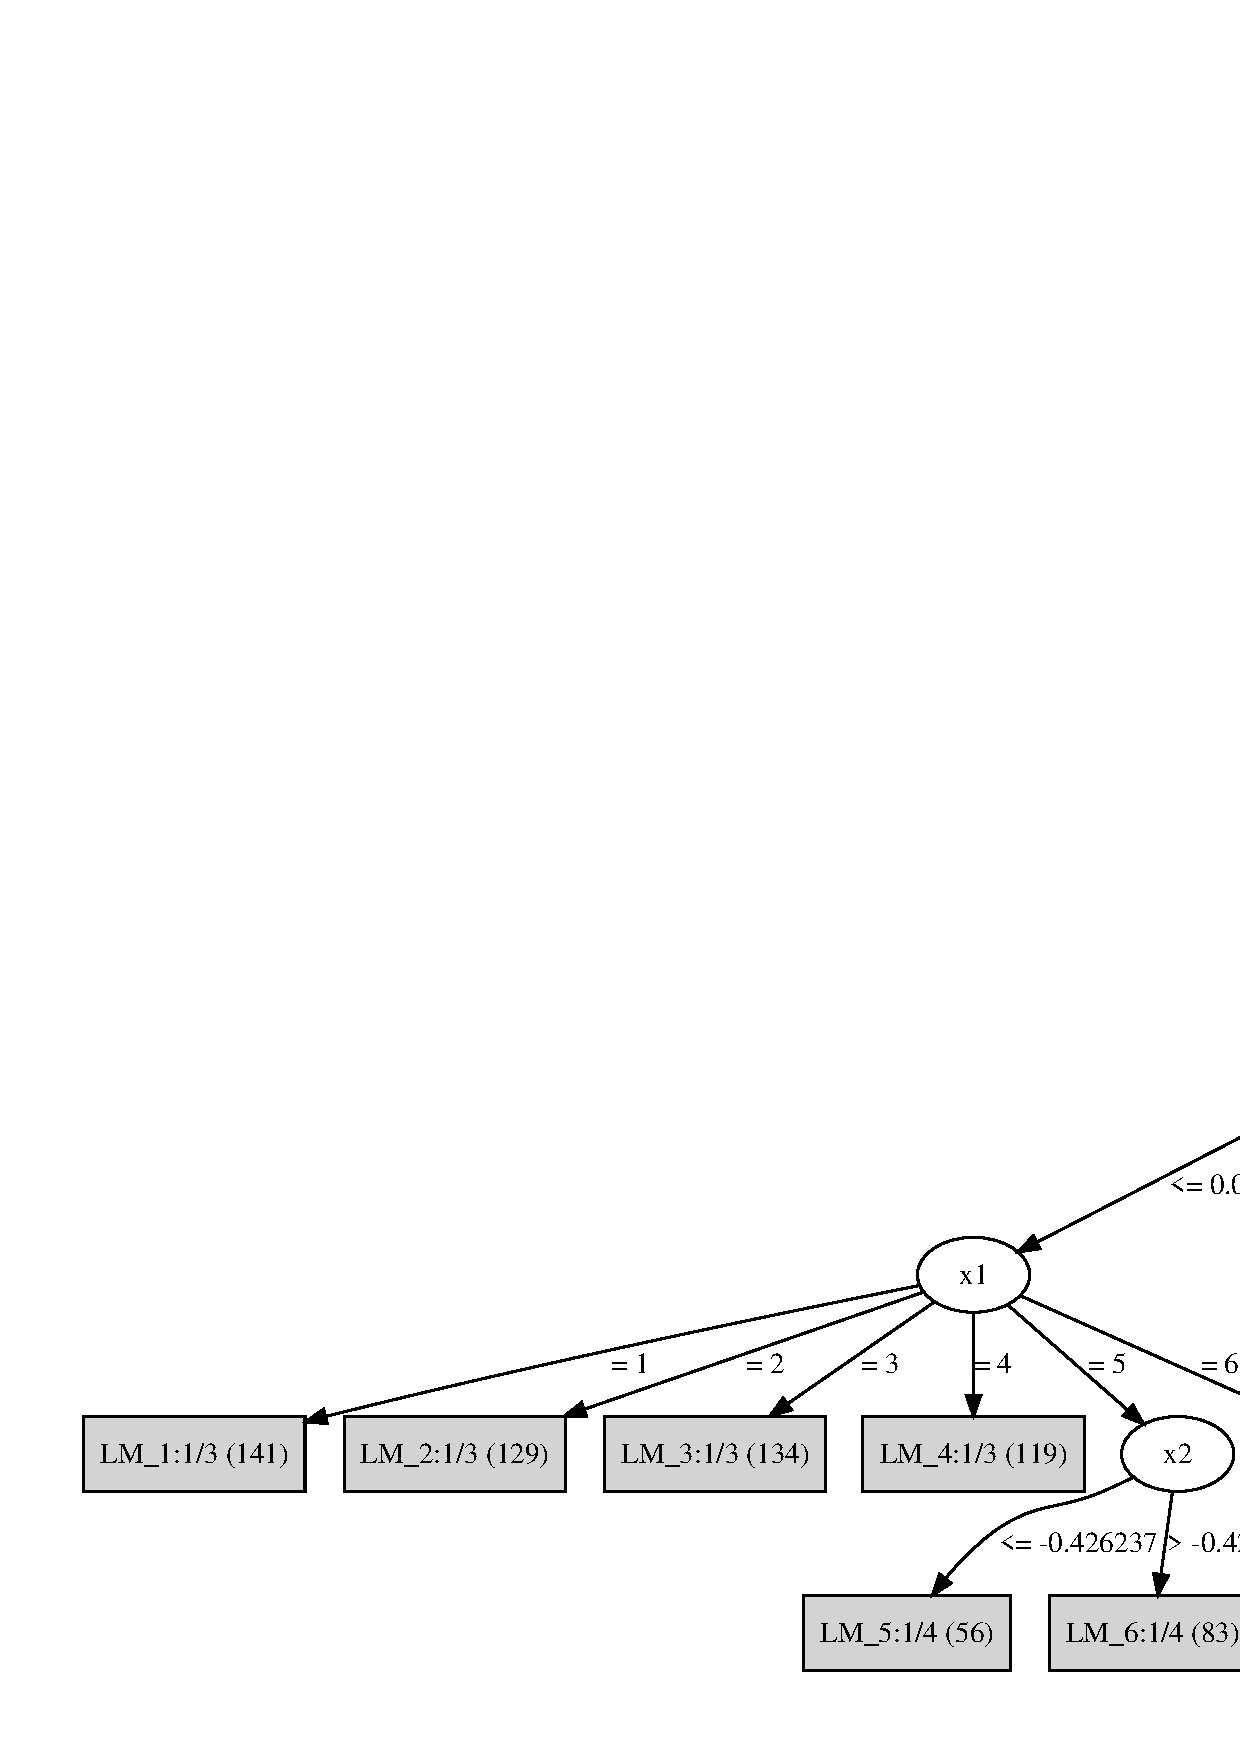
\includegraphics[scale=0.2]{R_CODE_FIGURES/chapitre6/graphLMT.png}
\caption{\gls{lmt} tree resulting from simulated data from (b).}
\label{fig:simu_b_lmt}
\end{figure}

\begin{figure}
\centering \resizebox{.7\textwidth}{!}{% Created by tikzDevice version 0.12 on 2019-03-21 20:20:43
% !TEX encoding = UTF-8 Unicode
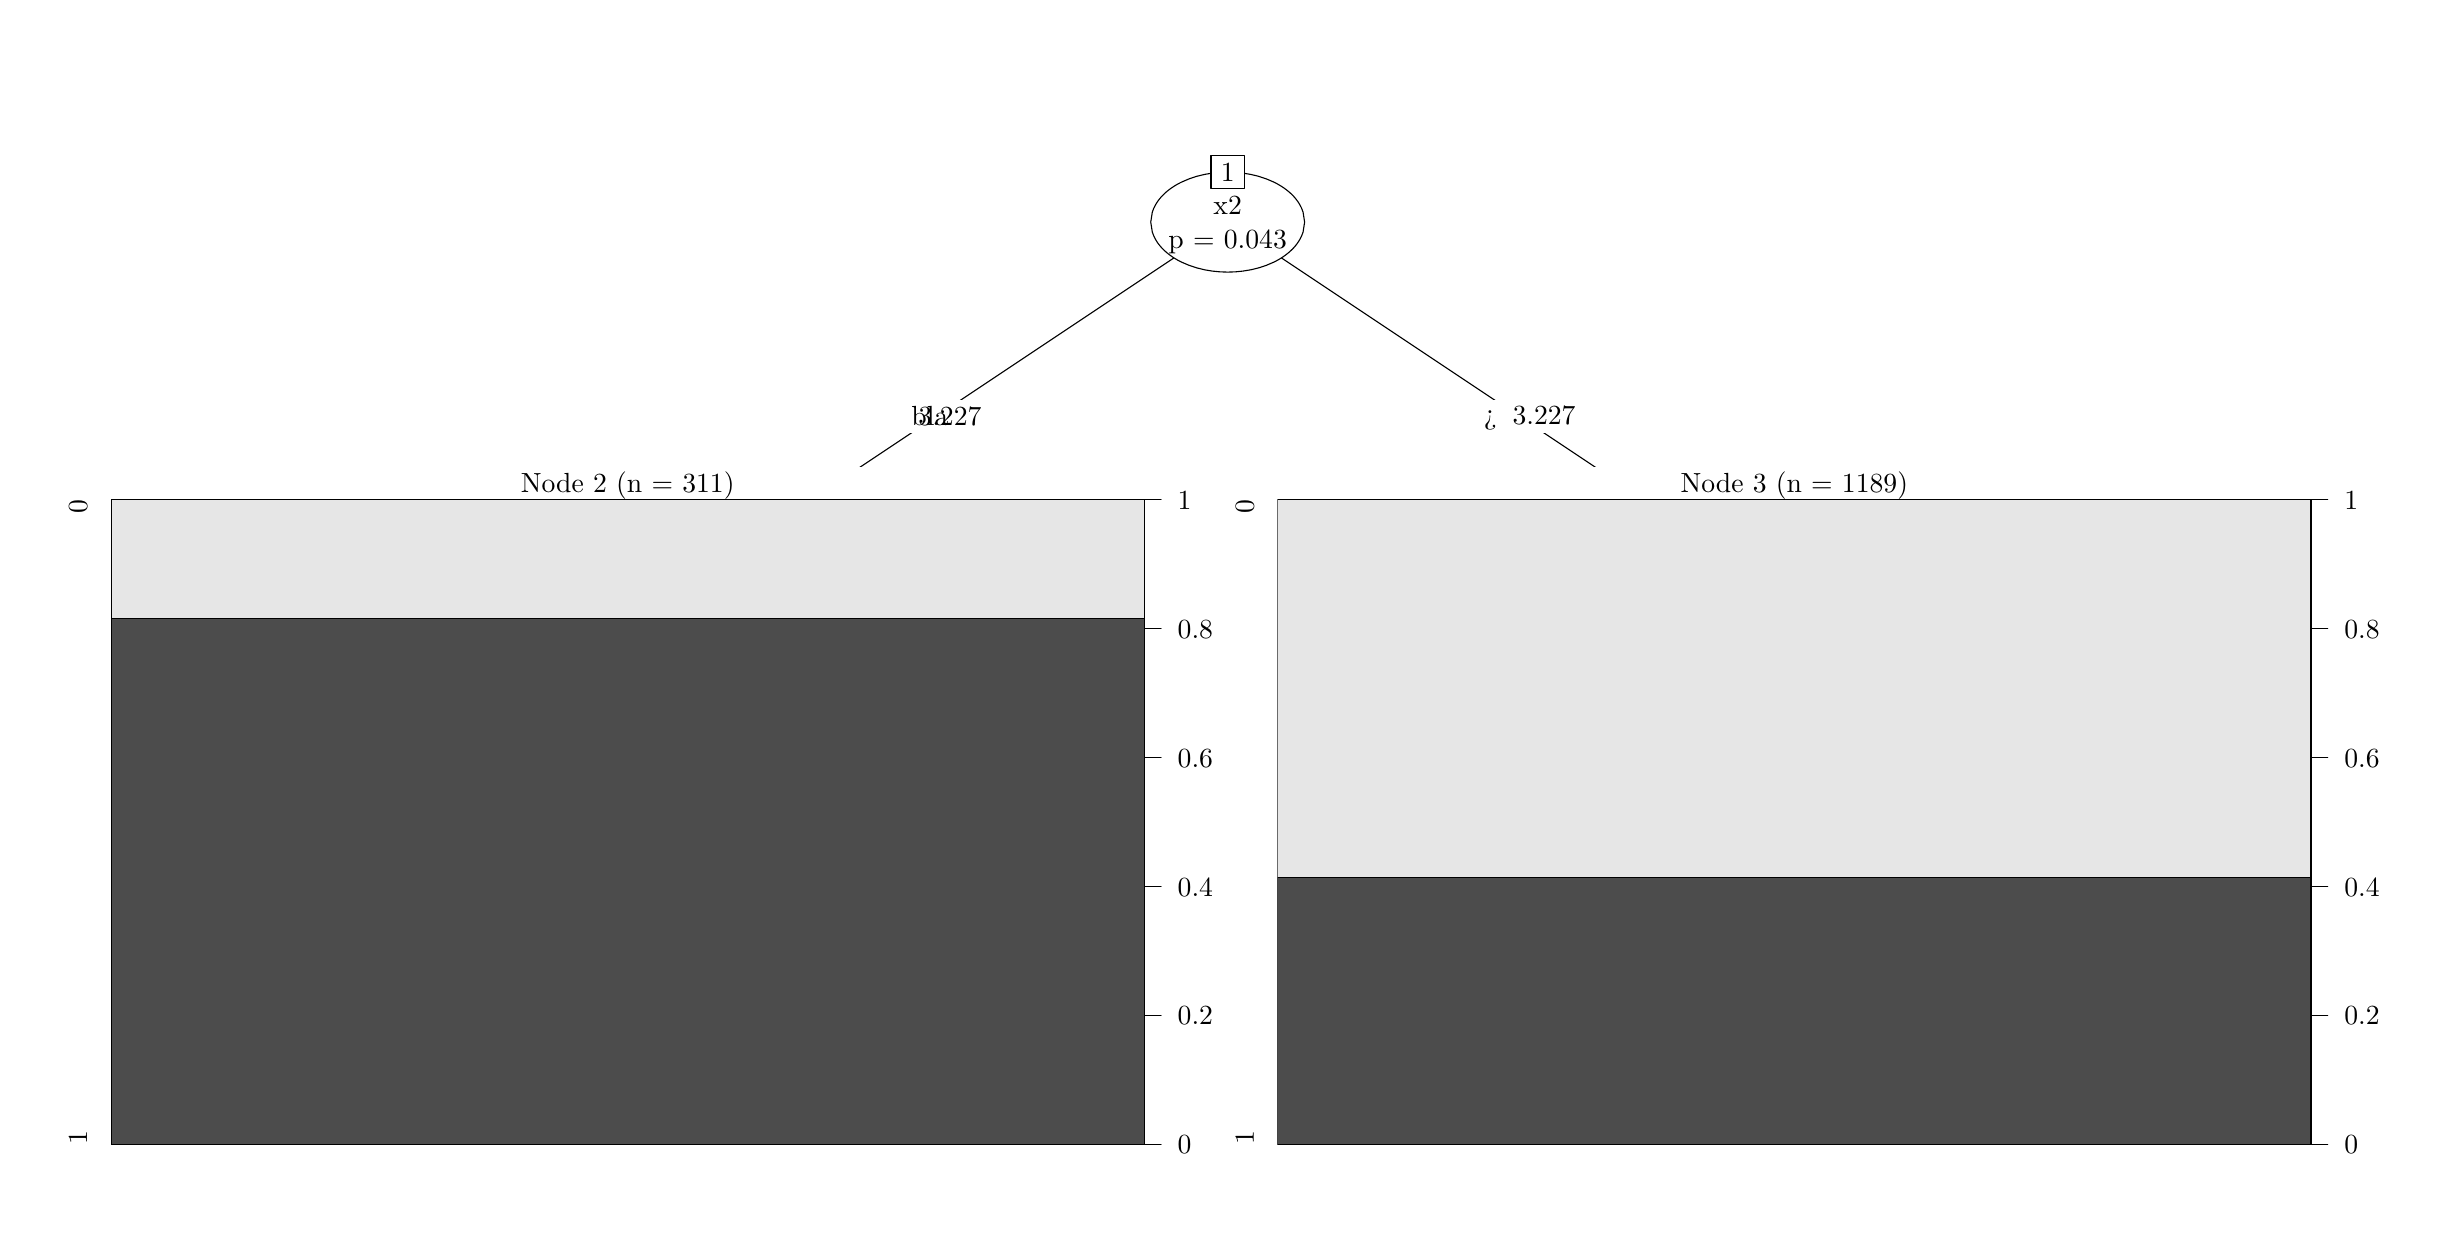
\begin{tikzpicture}[x=1pt,y=1pt]
\definecolor{fillColor}{RGB}{255,255,255}
\path[use as bounding box,fill=fillColor,fill opacity=0.00] (0,0) rectangle (867.24,433.62);
\begin{scope}
\path[clip] (  0.00,  0.00) rectangle (867.24,433.62);
\definecolor{drawColor}{RGB}{0,0,0}

\path[draw=drawColor,line width= 0.4pt,line join=round,line cap=round] (433.62,363.36) --
	(222.83,222.83);

\path[draw=drawColor,line width= 0.4pt,line join=round,line cap=round] (433.62,363.36) --
	(644.41,222.83);
\definecolor{fillColor}{RGB}{255,255,255}

\path[draw=drawColor,line width= 0.4pt,line join=round,line cap=round,fill=fillColor] (405.82,363.36) --
	(406.38,366.95) --
	(406.93,368.42) --
	(407.49,369.52) --
	(408.05,370.44) --
	(408.60,371.23) --
	(409.16,371.94) --
	(409.71,372.58) --
	(410.27,373.16) --
	(410.83,373.70) --
	(411.38,374.20) --
	(411.94,374.66) --
	(412.49,375.10) --
	(413.05,375.51) --
	(413.60,375.90) --
	(414.16,376.26) --
	(414.72,376.60) --
	(415.27,376.93) --
	(415.83,377.24) --
	(416.38,377.53) --
	(416.94,377.81) --
	(416.94,377.81) --
	(419.72,379.00) --
	(422.50,379.92) --
	(425.28,380.59) --
	(428.06,381.06) --
	(430.84,381.33) --
	(433.62,381.43) --
	(436.40,381.33) --
	(439.18,381.06) --
	(441.96,380.59) --
	(444.74,379.92) --
	(447.52,379.00) --
	(450.30,377.81) --
	(450.30,377.81) --
	(450.86,377.53) --
	(451.41,377.24) --
	(451.97,376.93) --
	(452.52,376.60) --
	(453.08,376.26) --
	(453.64,375.90) --
	(454.19,375.51) --
	(454.75,375.10) --
	(455.30,374.66) --
	(455.86,374.20) --
	(456.41,373.70) --
	(456.97,373.16) --
	(457.53,372.58) --
	(458.08,371.94) --
	(458.64,371.23) --
	(459.19,370.44) --
	(459.75,369.52) --
	(460.31,368.42) --
	(460.86,366.95) --
	(461.42,363.36) --
	(461.42,363.36) --
	(460.86,359.76) --
	(460.31,358.30) --
	(459.75,357.19) --
	(459.19,356.28) --
	(458.64,355.48) --
	(458.08,354.78) --
	(457.53,354.14) --
	(456.97,353.55) --
	(456.41,353.02) --
	(455.86,352.52) --
	(455.30,352.05) --
	(454.75,351.62) --
	(454.19,351.21) --
	(453.64,350.82) --
	(453.08,350.45) --
	(452.52,350.11) --
	(451.97,349.78) --
	(451.41,349.47) --
	(450.86,349.18) --
	(450.30,348.90) --
	(450.30,348.90) --
	(447.52,347.71) --
	(444.74,346.80) --
	(441.96,346.12) --
	(439.18,345.66) --
	(436.40,345.38) --
	(433.62,345.29) --
	(430.84,345.38) --
	(428.06,345.66) --
	(425.28,346.12) --
	(422.50,346.80) --
	(419.72,347.71) --
	(416.94,348.90) --
	(416.94,348.90) --
	(416.38,349.18) --
	(415.83,349.47) --
	(415.27,349.78) --
	(414.72,350.11) --
	(414.16,350.45) --
	(413.60,350.82) --
	(413.05,351.21) --
	(412.49,351.62) --
	(411.94,352.05) --
	(411.38,352.52) --
	(410.83,353.02) --
	(410.27,353.55) --
	(409.71,354.14) --
	(409.16,354.78) --
	(408.60,355.48) --
	(408.05,356.28) --
	(407.49,357.19) --
	(406.93,358.30) --
	(406.38,359.76) --
	(405.82,363.36) --
	cycle;

\node[text=drawColor,anchor=base,inner sep=0pt, outer sep=0pt, scale=  1.00] at (433.62,365.94) {x2};

\node[text=drawColor,anchor=base,inner sep=0pt, outer sep=0pt, scale=  1.00] at (433.62,353.89) {p = 0.043};

\path[draw=drawColor,line width= 0.4pt,line join=round,line cap=round,fill=fillColor] (427.60,375.40) rectangle (439.64,387.45);

\node[text=drawColor,anchor=base,inner sep=0pt, outer sep=0pt, scale=  1.00] at (433.62,377.98) {1};
\end{scope}
\begin{scope}
\path[clip] (  0.00,  0.00) rectangle (867.24,433.62);
\definecolor{fillColor}{RGB}{255,255,255}

\path[fill=fillColor] (311.80,287.07) rectangle (344.66,299.12);
\definecolor{drawColor}{RGB}{0,0,0}

\node[text=drawColor,anchor=base west,inner sep=0pt, outer sep=0pt, scale=  1.00] at (319.34,289.89) {bla};

\node[text=drawColor,anchor=base west,inner sep=0pt, outer sep=0pt, scale=  1.00] at (321.89,289.89) {3.227};
\end{scope}
\begin{scope}
\path[clip] (  0.00,  0.00) rectangle (867.24,433.62);
\definecolor{fillColor}{RGB}{255,255,255}

\path[fill=fillColor] (518.69,287.07) rectangle (559.33,299.12);
\definecolor{drawColor}{RGB}{0,0,0}

\node[text=drawColor,anchor=base west,inner sep=0pt, outer sep=0pt, scale=  1.00] at (526.24,290.08) {>};

\node[text=drawColor,anchor=base west,inner sep=0pt, outer sep=0pt, scale=  1.00] at (536.56,290.08) {3.227};
\end{scope}
\begin{scope}
\path[clip] (  0.00,  0.00) rectangle (867.24,433.62);
\definecolor{fillColor}{RGB}{255,255,255}

\path[fill=fillColor] ( 12.04, 30.11) rectangle (433.62,275.03);
\definecolor{drawColor}{RGB}{0,0,0}

\node[text=drawColor,anchor=base,inner sep=0pt, outer sep=0pt, scale=  1.00] at (216.81,265.56) {Node 2 (n = 311)};
\end{scope}
\begin{scope}
\path[clip] (  0.00,  0.00) rectangle (867.24,433.62);
\definecolor{drawColor}{RGB}{0,0,0}

\node[text=drawColor,rotate= 90.00,anchor=base west,inner sep=0pt, outer sep=0pt, scale=  1.00] at ( 21.51, 30.11) {1};

\node[text=drawColor,rotate= 90.00,anchor=base east,inner sep=0pt, outer sep=0pt, scale=  1.00] at ( 21.51,262.98) {0};

\path[draw=drawColor,line width= 0.4pt,line join=round,line cap=round] (403.51, 30.11) --
	(403.51,262.98);

\path[draw=drawColor,line width= 0.4pt,line join=round,line cap=round] (403.51, 30.11) -- (409.53, 30.11);

\path[draw=drawColor,line width= 0.4pt,line join=round,line cap=round] (403.51, 76.69) -- (409.53, 76.69);

\path[draw=drawColor,line width= 0.4pt,line join=round,line cap=round] (403.51,123.26) -- (409.53,123.26);

\path[draw=drawColor,line width= 0.4pt,line join=round,line cap=round] (403.51,169.83) -- (409.53,169.83);

\path[draw=drawColor,line width= 0.4pt,line join=round,line cap=round] (403.51,216.41) -- (409.53,216.41);

\path[draw=drawColor,line width= 0.4pt,line join=round,line cap=round] (403.51,262.98) -- (409.53,262.98);

\node[text=drawColor,anchor=base west,inner sep=0pt, outer sep=0pt, scale=  1.00] at (415.55, 26.67) {0};

\node[text=drawColor,anchor=base west,inner sep=0pt, outer sep=0pt, scale=  1.00] at (415.55, 73.24) {0.2};

\node[text=drawColor,anchor=base west,inner sep=0pt, outer sep=0pt, scale=  1.00] at (415.55,119.82) {0.4};

\node[text=drawColor,anchor=base west,inner sep=0pt, outer sep=0pt, scale=  1.00] at (415.55,166.39) {0.6};

\node[text=drawColor,anchor=base west,inner sep=0pt, outer sep=0pt, scale=  1.00] at (415.55,212.96) {0.8};

\node[text=drawColor,anchor=base west,inner sep=0pt, outer sep=0pt, scale=  1.00] at (415.55,259.54) {1};
\end{scope}
\begin{scope}
\path[clip] ( 30.11, 30.11) rectangle (403.51,262.98);
\definecolor{drawColor}{RGB}{0,0,0}

\path[draw=drawColor,line width= 0.4pt,line join=round,line cap=round] ( 30.11, 30.11) rectangle (403.51,262.98);
\definecolor{fillColor}{gray}{0.30}

\path[draw=drawColor,line width= 0.4pt,line join=round,line cap=round,fill=fillColor] ( 30.11, 30.11) rectangle (403.51,220.30);
\definecolor{fillColor}{RGB}{230,230,230}

\path[fill=fillColor] ( 30.11,220.30) rectangle (403.51,262.98);

\path[draw=drawColor,line width= 0.4pt,line join=round,line cap=round] ( 30.11, 30.11) rectangle (403.51,262.98);
\end{scope}
\begin{scope}
\path[clip] (  0.00,  0.00) rectangle (867.24,433.62);
\definecolor{fillColor}{RGB}{255,255,255}

\path[fill=fillColor] (433.62, 30.11) rectangle (855.20,275.03);
\definecolor{drawColor}{RGB}{0,0,0}

\node[text=drawColor,anchor=base,inner sep=0pt, outer sep=0pt, scale=  1.00] at (638.38,265.56) {Node 3 (n = 1189)};
\end{scope}
\begin{scope}
\path[clip] (  0.00,  0.00) rectangle (867.24,433.62);
\definecolor{drawColor}{RGB}{0,0,0}

\node[text=drawColor,rotate= 90.00,anchor=base west,inner sep=0pt, outer sep=0pt, scale=  1.00] at (443.09, 30.11) {1};

\node[text=drawColor,rotate= 90.00,anchor=base east,inner sep=0pt, outer sep=0pt, scale=  1.00] at (443.09,262.98) {0};

\path[draw=drawColor,line width= 0.4pt,line join=round,line cap=round] (825.08, 30.11) --
	(825.08,262.98);

\path[draw=drawColor,line width= 0.4pt,line join=round,line cap=round] (825.08, 30.11) -- (831.11, 30.11);

\path[draw=drawColor,line width= 0.4pt,line join=round,line cap=round] (825.08, 76.69) -- (831.11, 76.69);

\path[draw=drawColor,line width= 0.4pt,line join=round,line cap=round] (825.08,123.26) -- (831.11,123.26);

\path[draw=drawColor,line width= 0.4pt,line join=round,line cap=round] (825.08,169.83) -- (831.11,169.83);

\path[draw=drawColor,line width= 0.4pt,line join=round,line cap=round] (825.08,216.41) -- (831.11,216.41);

\path[draw=drawColor,line width= 0.4pt,line join=round,line cap=round] (825.08,262.98) -- (831.11,262.98);

\node[text=drawColor,anchor=base west,inner sep=0pt, outer sep=0pt, scale=  1.00] at (837.13, 26.67) {0};

\node[text=drawColor,anchor=base west,inner sep=0pt, outer sep=0pt, scale=  1.00] at (837.13, 73.24) {0.2};

\node[text=drawColor,anchor=base west,inner sep=0pt, outer sep=0pt, scale=  1.00] at (837.13,119.82) {0.4};

\node[text=drawColor,anchor=base west,inner sep=0pt, outer sep=0pt, scale=  1.00] at (837.13,166.39) {0.6};

\node[text=drawColor,anchor=base west,inner sep=0pt, outer sep=0pt, scale=  1.00] at (837.13,212.96) {0.8};

\node[text=drawColor,anchor=base west,inner sep=0pt, outer sep=0pt, scale=  1.00] at (837.13,259.54) {1};
\end{scope}
\begin{scope}
\path[clip] (451.69, 30.11) rectangle (825.08,262.98);
\definecolor{drawColor}{RGB}{0,0,0}

\path[draw=drawColor,line width= 0.4pt,line join=round,line cap=round] (451.69, 30.11) rectangle (825.08,262.98);
\definecolor{fillColor}{gray}{0.30}

\path[draw=drawColor,line width= 0.4pt,line join=round,line cap=round,fill=fillColor] (451.69, 30.11) rectangle (825.08,126.67);
\definecolor{fillColor}{RGB}{230,230,230}

\path[fill=fillColor] (451.69,126.67) rectangle (825.08,262.98);

\path[draw=drawColor,line width= 0.4pt,line join=round,line cap=round] (451.69, 30.11) rectangle (825.08,262.98);
\end{scope}
\end{tikzpicture}
}
\caption{\gls{mob} tree resulting from simulated data from (a).}
\label{fig:simu_a_mob}
\end{figure}

\begin{figure}
\centering \resizebox{.7\textwidth}{!}{% Created by tikzDevice version 0.12 on 2019-03-21 22:03:49
% !TEX encoding = UTF-8 Unicode
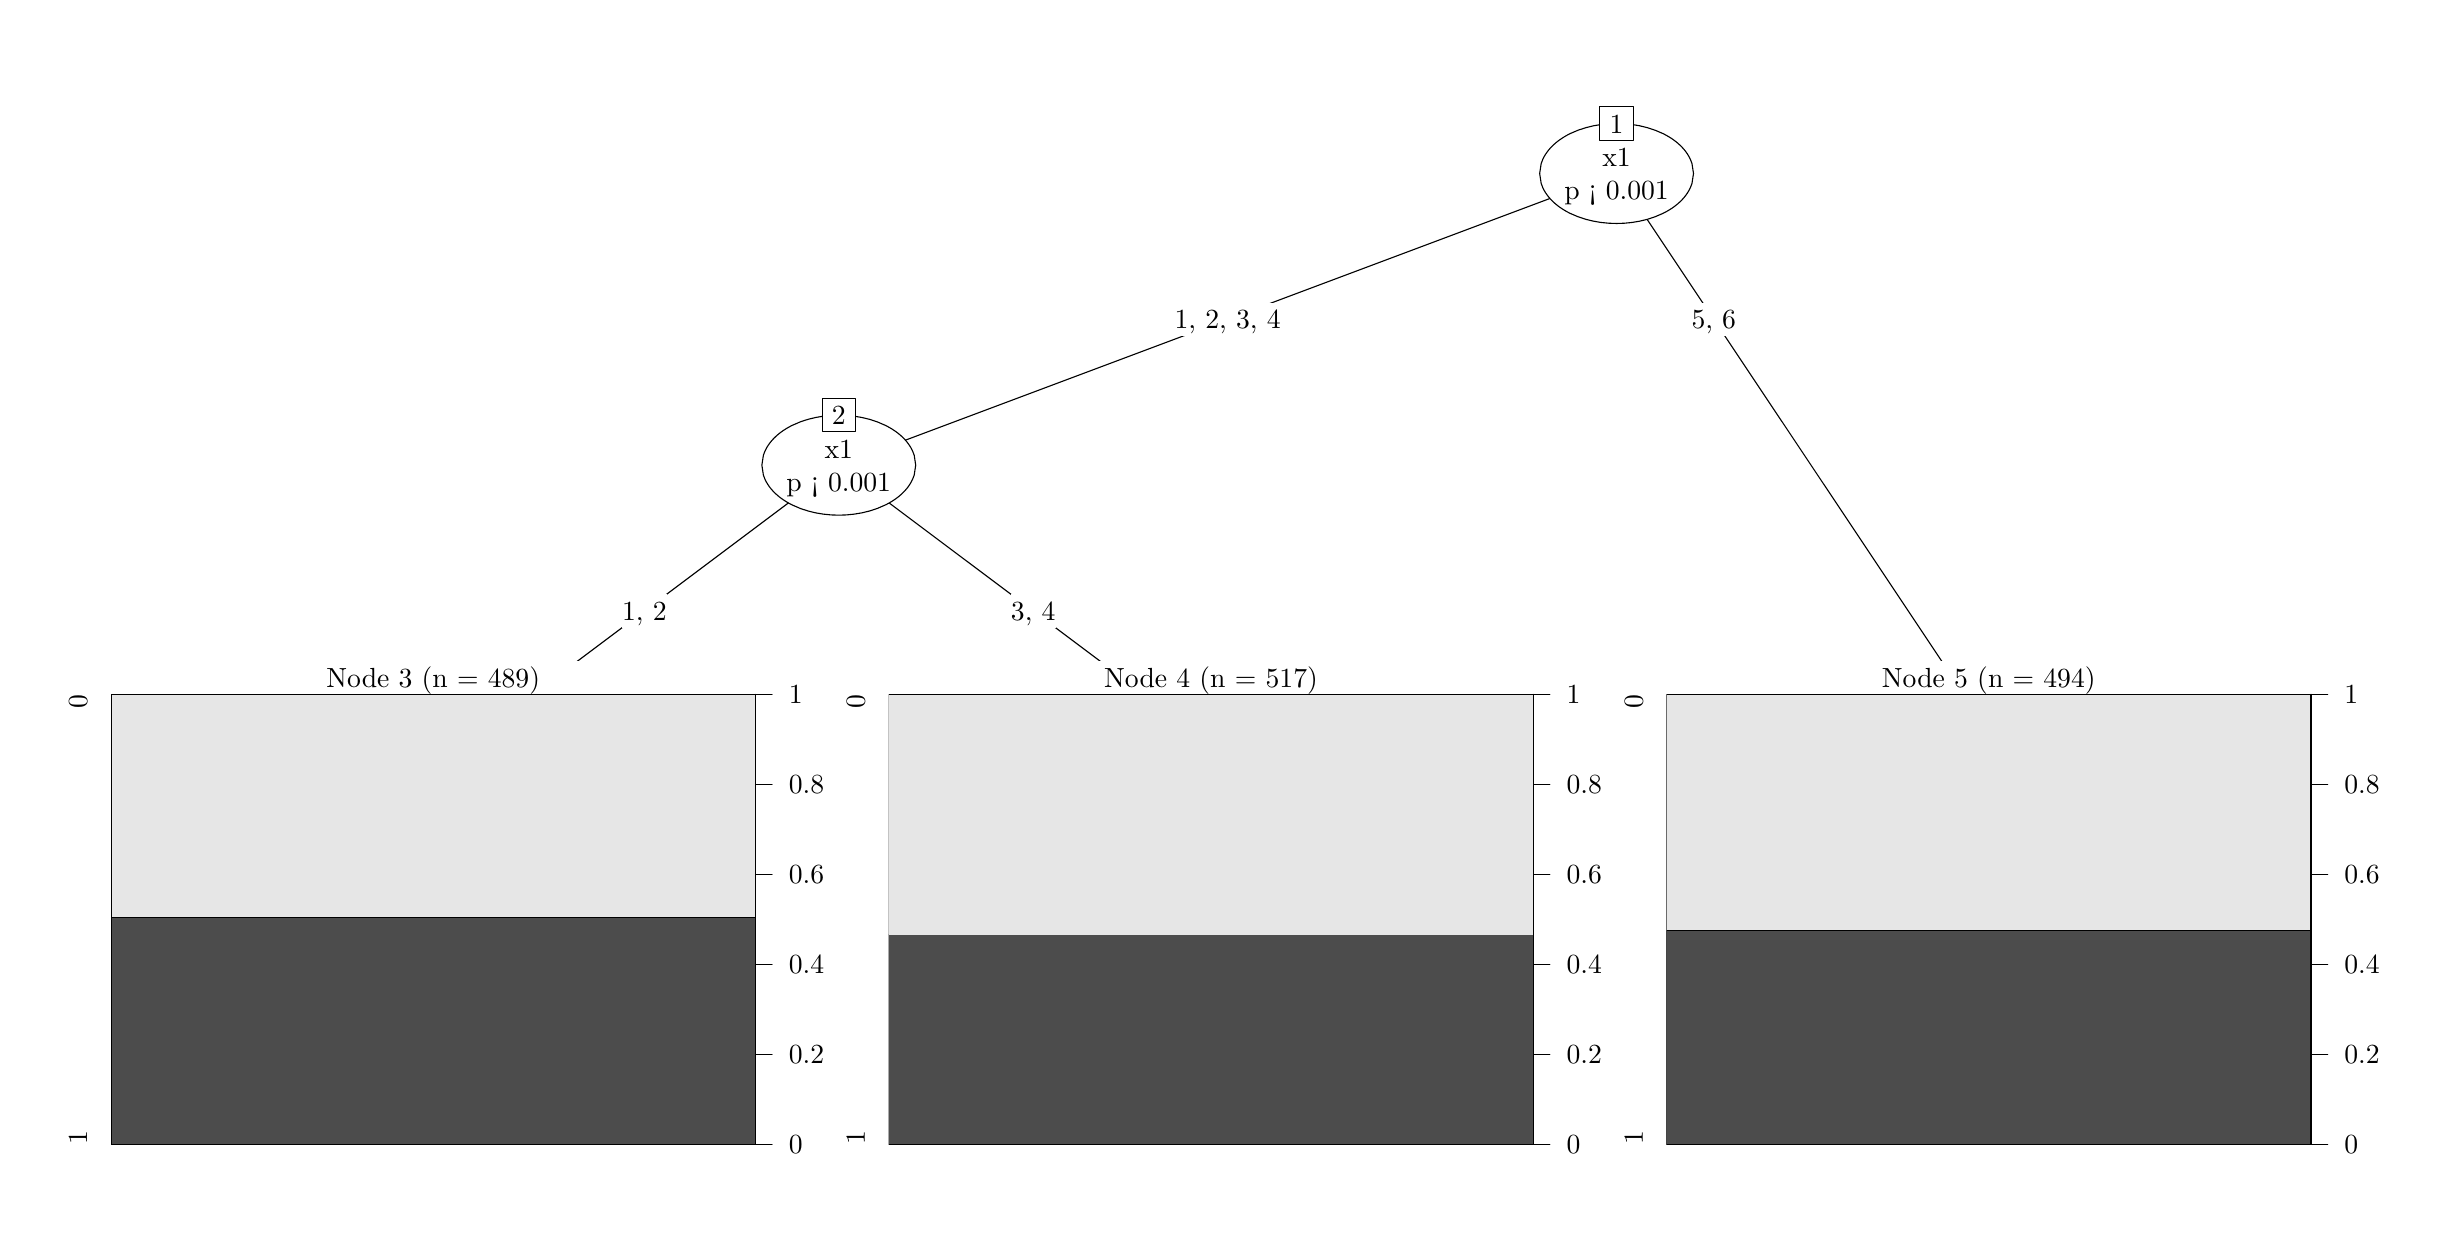
\begin{tikzpicture}[x=1pt,y=1pt]
\definecolor{fillColor}{RGB}{255,255,255}
\path[use as bounding box,fill=fillColor,fill opacity=0.00] (0,0) rectangle (867.24,433.62);
\begin{scope}
\path[clip] (  0.00,  0.00) rectangle (867.24,433.62);
\definecolor{drawColor}{RGB}{0,0,0}

\path[draw=drawColor,line width= 0.4pt,line join=round,line cap=round] (574.14,380.92) --
	(293.09,275.53);

\path[draw=drawColor,line width= 0.4pt,line join=round,line cap=round] (574.14,380.92) --
	(714.67,170.14);
\definecolor{fillColor}{RGB}{255,255,255}

\path[draw=drawColor,line width= 0.4pt,line join=round,line cap=round,fill=fillColor] (546.35,380.92) --
	(546.90,384.52) --
	(547.46,385.98) --
	(548.01,387.09) --
	(548.57,388.00) --
	(549.13,388.80) --
	(549.68,389.50) --
	(550.24,390.14) --
	(550.79,390.73) --
	(551.35,391.26) --
	(551.91,391.76) --
	(552.46,392.23) --
	(553.02,392.67) --
	(553.57,393.08) --
	(554.13,393.46) --
	(554.69,393.83) --
	(555.24,394.17) --
	(555.80,394.50) --
	(556.35,394.81) --
	(556.91,395.10) --
	(557.47,395.38) --
	(557.47,395.38) --
	(560.25,396.57) --
	(563.03,397.48) --
	(565.81,398.16) --
	(568.59,398.63) --
	(571.37,398.90) --
	(574.14,398.99) --
	(576.92,398.90) --
	(579.70,398.63) --
	(582.48,398.16) --
	(585.26,397.48) --
	(588.04,396.57) --
	(590.82,395.38) --
	(590.82,395.38) --
	(591.38,395.10) --
	(591.94,394.81) --
	(592.49,394.50) --
	(593.05,394.17) --
	(593.60,393.83) --
	(594.16,393.46) --
	(594.72,393.08) --
	(595.27,392.67) --
	(595.83,392.23) --
	(596.38,391.76) --
	(596.94,391.26) --
	(597.50,390.73) --
	(598.05,390.14) --
	(598.61,389.50) --
	(599.16,388.80) --
	(599.72,388.00) --
	(600.28,387.09) --
	(600.83,385.98) --
	(601.39,384.52) --
	(601.94,380.92) --
	(601.94,380.92) --
	(601.39,377.33) --
	(600.83,375.86) --
	(600.28,374.76) --
	(599.72,373.84) --
	(599.16,373.05) --
	(598.61,372.34) --
	(598.05,371.70) --
	(597.50,371.12) --
	(596.94,370.58) --
	(596.38,370.08) --
	(595.83,369.62) --
	(595.27,369.18) --
	(594.72,368.77) --
	(594.16,368.38) --
	(593.60,368.02) --
	(593.05,367.68) --
	(592.49,367.35) --
	(591.94,367.04) --
	(591.38,366.75) --
	(590.82,366.47) --
	(590.82,366.47) --
	(588.04,365.28) --
	(585.26,364.36) --
	(582.48,363.69) --
	(579.70,363.22) --
	(576.92,362.95) --
	(574.14,362.86) --
	(571.37,362.95) --
	(568.59,363.22) --
	(565.81,363.69) --
	(563.03,364.36) --
	(560.25,365.28) --
	(557.47,366.47) --
	(557.47,366.47) --
	(556.91,366.75) --
	(556.35,367.04) --
	(555.80,367.35) --
	(555.24,367.68) --
	(554.69,368.02) --
	(554.13,368.38) --
	(553.57,368.77) --
	(553.02,369.18) --
	(552.46,369.62) --
	(551.91,370.08) --
	(551.35,370.58) --
	(550.79,371.12) --
	(550.24,371.70) --
	(549.68,372.34) --
	(549.13,373.05) --
	(548.57,373.84) --
	(548.01,374.76) --
	(547.46,375.86) --
	(546.90,377.33) --
	(546.35,380.92) --
	cycle;

\node[text=drawColor,anchor=base,inner sep=0pt, outer sep=0pt, scale=  1.00] at (574.14,383.50) {x1};

\node[text=drawColor,anchor=base,inner sep=0pt, outer sep=0pt, scale=  1.00] at (574.14,371.46) {p < 0.001};

\path[draw=drawColor,line width= 0.4pt,line join=round,line cap=round,fill=fillColor] (568.12,392.97) rectangle (580.17,405.01);

\node[text=drawColor,anchor=base,inner sep=0pt, outer sep=0pt, scale=  1.00] at (574.14,395.55) {1};
\end{scope}
\begin{scope}
\path[clip] (  0.00,  0.00) rectangle (867.24,433.62);
\definecolor{fillColor}{RGB}{255,255,255}

\path[fill=fillColor] (414.46,322.20) rectangle (452.78,334.25);
\definecolor{drawColor}{RGB}{0,0,0}

\node[text=drawColor,anchor=base,inner sep=0pt, outer sep=0pt, scale=  1.00] at (433.62,324.78) {1, 2, 3, 4};
\end{scope}
\begin{scope}
\path[clip] (  0.00,  0.00) rectangle (867.24,433.62);
\definecolor{fillColor}{RGB}{255,255,255}

\path[fill=fillColor] (601.22,322.20) rectangle (617.33,334.25);
\definecolor{drawColor}{RGB}{0,0,0}

\node[text=drawColor,anchor=base,inner sep=0pt, outer sep=0pt, scale=  1.00] at (609.28,324.78) {5, 6};
\end{scope}
\begin{scope}
\path[clip] (  0.00,  0.00) rectangle (867.24,433.62);
\definecolor{drawColor}{RGB}{0,0,0}

\path[draw=drawColor,line width= 0.4pt,line join=round,line cap=round] (293.09,275.53) --
	(152.57,170.14);

\path[draw=drawColor,line width= 0.4pt,line join=round,line cap=round] (293.09,275.53) --
	(433.62,170.14);
\definecolor{fillColor}{RGB}{255,255,255}

\path[draw=drawColor,line width= 0.4pt,line join=round,line cap=round,fill=fillColor] (265.30,275.53) --
	(265.85,279.12) --
	(266.41,280.59) --
	(266.96,281.69) --
	(267.52,282.61) --
	(268.08,283.40) --
	(268.63,284.11) --
	(269.19,284.75) --
	(269.74,285.33) --
	(270.30,285.87) --
	(270.86,286.37) --
	(271.41,286.84) --
	(271.97,287.27) --
	(272.52,287.68) --
	(273.08,288.07) --
	(273.64,288.43) --
	(274.19,288.78) --
	(274.75,289.10) --
	(275.30,289.41) --
	(275.86,289.71) --
	(276.42,289.98) --
	(276.42,289.98) --
	(279.20,291.18) --
	(281.98,292.09) --
	(284.76,292.76) --
	(287.54,293.23) --
	(290.32,293.51) --
	(293.09,293.60) --
	(295.87,293.51) --
	(298.65,293.23) --
	(301.43,292.76) --
	(304.21,292.09) --
	(306.99,291.18) --
	(309.77,289.98) --
	(309.77,289.98) --
	(310.33,289.71) --
	(310.89,289.41) --
	(311.44,289.10) --
	(312.00,288.78) --
	(312.55,288.43) --
	(313.11,288.07) --
	(313.67,287.68) --
	(314.22,287.27) --
	(314.78,286.84) --
	(315.33,286.37) --
	(315.89,285.87) --
	(316.45,285.33) --
	(317.00,284.75) --
	(317.56,284.11) --
	(318.11,283.40) --
	(318.67,282.61) --
	(319.23,281.69) --
	(319.78,280.59) --
	(320.34,279.12) --
	(320.89,275.53) --
	(320.89,275.53) --
	(320.34,271.93) --
	(319.78,270.47) --
	(319.23,269.37) --
	(318.67,268.45) --
	(318.11,267.65) --
	(317.56,266.95) --
	(317.00,266.31) --
	(316.45,265.73) --
	(315.89,265.19) --
	(315.33,264.69) --
	(314.78,264.22) --
	(314.22,263.79) --
	(313.67,263.38) --
	(313.11,262.99) --
	(312.55,262.63) --
	(312.00,262.28) --
	(311.44,261.96) --
	(310.89,261.65) --
	(310.33,261.35) --
	(309.77,261.08) --
	(309.77,261.08) --
	(306.99,259.88) --
	(304.21,258.97) --
	(301.43,258.29) --
	(298.65,257.83) --
	(295.87,257.55) --
	(293.09,257.46) --
	(290.32,257.55) --
	(287.54,257.83) --
	(284.76,258.29) --
	(281.98,258.97) --
	(279.20,259.88) --
	(276.42,261.08) --
	(276.42,261.08) --
	(275.86,261.35) --
	(275.30,261.65) --
	(274.75,261.96) --
	(274.19,262.28) --
	(273.64,262.63) --
	(273.08,262.99) --
	(272.52,263.38) --
	(271.97,263.79) --
	(271.41,264.22) --
	(270.86,264.69) --
	(270.30,265.19) --
	(269.74,265.73) --
	(269.19,266.31) --
	(268.63,266.95) --
	(268.08,267.65) --
	(267.52,268.45) --
	(266.96,269.37) --
	(266.41,270.47) --
	(265.85,271.93) --
	(265.30,275.53) --
	cycle;

\node[text=drawColor,anchor=base,inner sep=0pt, outer sep=0pt, scale=  1.00] at (293.09,278.11) {x1};

\node[text=drawColor,anchor=base,inner sep=0pt, outer sep=0pt, scale=  1.00] at (293.09,266.06) {p < 0.001};

\path[draw=drawColor,line width= 0.4pt,line join=round,line cap=round,fill=fillColor] (287.07,287.57) rectangle (299.12,299.62);

\node[text=drawColor,anchor=base,inner sep=0pt, outer sep=0pt, scale=  1.00] at (293.09,290.15) {2};
\end{scope}
\begin{scope}
\path[clip] (  0.00,  0.00) rectangle (867.24,433.62);
\definecolor{fillColor}{RGB}{255,255,255}

\path[fill=fillColor] (214.78,216.81) rectangle (230.89,228.85);
\definecolor{drawColor}{RGB}{0,0,0}

\node[text=drawColor,anchor=base,inner sep=0pt, outer sep=0pt, scale=  1.00] at (222.83,219.39) {1, 2};
\end{scope}
\begin{scope}
\path[clip] (  0.00,  0.00) rectangle (867.24,433.62);
\definecolor{fillColor}{RGB}{255,255,255}

\path[fill=fillColor] (355.30,216.81) rectangle (371.41,228.85);
\definecolor{drawColor}{RGB}{0,0,0}

\node[text=drawColor,anchor=base,inner sep=0pt, outer sep=0pt, scale=  1.00] at (363.36,219.39) {3, 4};
\end{scope}
\begin{scope}
\path[clip] (  0.00,  0.00) rectangle (867.24,433.62);
\definecolor{fillColor}{RGB}{255,255,255}

\path[fill=fillColor] ( 12.05, 30.11) rectangle (293.10,204.76);
\definecolor{drawColor}{RGB}{0,0,0}

\node[text=drawColor,anchor=base,inner sep=0pt, outer sep=0pt, scale=  1.00] at (146.55,195.30) {Node 3 (n = 489)};
\end{scope}
\begin{scope}
\path[clip] (  0.00,  0.00) rectangle (867.24,433.62);
\definecolor{drawColor}{RGB}{0,0,0}

\node[text=drawColor,rotate= 90.00,anchor=base west,inner sep=0pt, outer sep=0pt, scale=  1.00] at ( 21.51, 30.11) {1};

\node[text=drawColor,rotate= 90.00,anchor=base east,inner sep=0pt, outer sep=0pt, scale=  1.00] at ( 21.51,192.72) {0};

\path[draw=drawColor,line width= 0.4pt,line join=round,line cap=round] (262.98, 30.11) --
	(262.98,192.72);

\path[draw=drawColor,line width= 0.4pt,line join=round,line cap=round] (262.98, 30.11) -- (269.00, 30.11);

\path[draw=drawColor,line width= 0.4pt,line join=round,line cap=round] (262.98, 62.63) -- (269.00, 62.63);

\path[draw=drawColor,line width= 0.4pt,line join=round,line cap=round] (262.98, 95.16) -- (269.00, 95.16);

\path[draw=drawColor,line width= 0.4pt,line join=round,line cap=round] (262.98,127.68) -- (269.00,127.68);

\path[draw=drawColor,line width= 0.4pt,line join=round,line cap=round] (262.98,160.20) -- (269.00,160.20);

\path[draw=drawColor,line width= 0.4pt,line join=round,line cap=round] (262.98,192.72) -- (269.00,192.72);

\node[text=drawColor,anchor=base west,inner sep=0pt, outer sep=0pt, scale=  1.00] at (275.03, 26.67) {0};

\node[text=drawColor,anchor=base west,inner sep=0pt, outer sep=0pt, scale=  1.00] at (275.03, 59.19) {0.2};

\node[text=drawColor,anchor=base west,inner sep=0pt, outer sep=0pt, scale=  1.00] at (275.03, 91.71) {0.4};

\node[text=drawColor,anchor=base west,inner sep=0pt, outer sep=0pt, scale=  1.00] at (275.03,124.23) {0.6};

\node[text=drawColor,anchor=base west,inner sep=0pt, outer sep=0pt, scale=  1.00] at (275.03,156.75) {0.8};

\node[text=drawColor,anchor=base west,inner sep=0pt, outer sep=0pt, scale=  1.00] at (275.03,189.28) {1};
\end{scope}
\begin{scope}
\path[clip] ( 30.11, 30.11) rectangle (262.98,192.72);
\definecolor{drawColor}{RGB}{0,0,0}

\path[draw=drawColor,line width= 0.4pt,line join=round,line cap=round] ( 30.11, 30.11) rectangle (262.98,192.72);
\definecolor{fillColor}{gray}{0.30}

\path[draw=drawColor,line width= 0.4pt,line join=round,line cap=round,fill=fillColor] ( 30.11, 30.11) rectangle (262.98,112.25);
\definecolor{fillColor}{RGB}{230,230,230}

\path[fill=fillColor] ( 30.11,112.25) rectangle (262.98,192.72);

\path[draw=drawColor,line width= 0.4pt,line join=round,line cap=round] ( 30.11, 30.11) rectangle (262.98,192.72);
\end{scope}
\begin{scope}
\path[clip] (  0.00,  0.00) rectangle (867.24,433.62);
\definecolor{fillColor}{RGB}{255,255,255}

\path[fill=fillColor] (293.10, 30.11) rectangle (574.14,204.76);
\definecolor{drawColor}{RGB}{0,0,0}

\node[text=drawColor,anchor=base,inner sep=0pt, outer sep=0pt, scale=  1.00] at (427.60,195.30) {Node 4 (n = 517)};
\end{scope}
\begin{scope}
\path[clip] (  0.00,  0.00) rectangle (867.24,433.62);
\definecolor{drawColor}{RGB}{0,0,0}

\node[text=drawColor,rotate= 90.00,anchor=base west,inner sep=0pt, outer sep=0pt, scale=  1.00] at (302.56, 30.11) {1};

\node[text=drawColor,rotate= 90.00,anchor=base east,inner sep=0pt, outer sep=0pt, scale=  1.00] at (302.56,192.72) {0};

\path[draw=drawColor,line width= 0.4pt,line join=round,line cap=round] (544.03, 30.11) --
	(544.03,192.72);

\path[draw=drawColor,line width= 0.4pt,line join=round,line cap=round] (544.03, 30.11) -- (550.06, 30.11);

\path[draw=drawColor,line width= 0.4pt,line join=round,line cap=round] (544.03, 62.63) -- (550.06, 62.63);

\path[draw=drawColor,line width= 0.4pt,line join=round,line cap=round] (544.03, 95.16) -- (550.06, 95.16);

\path[draw=drawColor,line width= 0.4pt,line join=round,line cap=round] (544.03,127.68) -- (550.06,127.68);

\path[draw=drawColor,line width= 0.4pt,line join=round,line cap=round] (544.03,160.20) -- (550.06,160.20);

\path[draw=drawColor,line width= 0.4pt,line join=round,line cap=round] (544.03,192.72) -- (550.06,192.72);

\node[text=drawColor,anchor=base west,inner sep=0pt, outer sep=0pt, scale=  1.00] at (556.08, 26.67) {0};

\node[text=drawColor,anchor=base west,inner sep=0pt, outer sep=0pt, scale=  1.00] at (556.08, 59.19) {0.2};

\node[text=drawColor,anchor=base west,inner sep=0pt, outer sep=0pt, scale=  1.00] at (556.08, 91.71) {0.4};

\node[text=drawColor,anchor=base west,inner sep=0pt, outer sep=0pt, scale=  1.00] at (556.08,124.23) {0.6};

\node[text=drawColor,anchor=base west,inner sep=0pt, outer sep=0pt, scale=  1.00] at (556.08,156.75) {0.8};

\node[text=drawColor,anchor=base west,inner sep=0pt, outer sep=0pt, scale=  1.00] at (556.08,189.28) {1};
\end{scope}
\begin{scope}
\path[clip] (311.16, 30.11) rectangle (544.03,192.72);
\definecolor{drawColor}{RGB}{0,0,0}

\path[draw=drawColor,line width= 0.4pt,line join=round,line cap=round] (311.16, 30.11) rectangle (544.03,192.72);
\definecolor{fillColor}{gray}{0.30}

\path[draw=drawColor,line width= 0.4pt,line join=round,line cap=round,fill=fillColor] (311.16, 30.11) rectangle (544.03,105.91);
\definecolor{fillColor}{RGB}{230,230,230}

\path[fill=fillColor] (311.16,105.91) rectangle (544.03,192.72);

\path[draw=drawColor,line width= 0.4pt,line join=round,line cap=round] (311.16, 30.11) rectangle (544.03,192.72);
\end{scope}
\begin{scope}
\path[clip] (  0.00,  0.00) rectangle (867.24,433.62);
\definecolor{fillColor}{RGB}{255,255,255}

\path[fill=fillColor] (574.14, 30.11) rectangle (855.19,204.76);
\definecolor{drawColor}{RGB}{0,0,0}

\node[text=drawColor,anchor=base,inner sep=0pt, outer sep=0pt, scale=  1.00] at (708.65,195.30) {Node 5 (n = 494)};
\end{scope}
\begin{scope}
\path[clip] (  0.00,  0.00) rectangle (867.24,433.62);
\definecolor{drawColor}{RGB}{0,0,0}

\node[text=drawColor,rotate= 90.00,anchor=base west,inner sep=0pt, outer sep=0pt, scale=  1.00] at (583.61, 30.11) {1};

\node[text=drawColor,rotate= 90.00,anchor=base east,inner sep=0pt, outer sep=0pt, scale=  1.00] at (583.61,192.72) {0};

\path[draw=drawColor,line width= 0.4pt,line join=round,line cap=round] (825.08, 30.11) --
	(825.08,192.72);

\path[draw=drawColor,line width= 0.4pt,line join=round,line cap=round] (825.08, 30.11) -- (831.11, 30.11);

\path[draw=drawColor,line width= 0.4pt,line join=round,line cap=round] (825.08, 62.63) -- (831.11, 62.63);

\path[draw=drawColor,line width= 0.4pt,line join=round,line cap=round] (825.08, 95.16) -- (831.11, 95.16);

\path[draw=drawColor,line width= 0.4pt,line join=round,line cap=round] (825.08,127.68) -- (831.11,127.68);

\path[draw=drawColor,line width= 0.4pt,line join=round,line cap=round] (825.08,160.20) -- (831.11,160.20);

\path[draw=drawColor,line width= 0.4pt,line join=round,line cap=round] (825.08,192.72) -- (831.11,192.72);

\node[text=drawColor,anchor=base west,inner sep=0pt, outer sep=0pt, scale=  1.00] at (837.13, 26.67) {0};

\node[text=drawColor,anchor=base west,inner sep=0pt, outer sep=0pt, scale=  1.00] at (837.13, 59.19) {0.2};

\node[text=drawColor,anchor=base west,inner sep=0pt, outer sep=0pt, scale=  1.00] at (837.13, 91.71) {0.4};

\node[text=drawColor,anchor=base west,inner sep=0pt, outer sep=0pt, scale=  1.00] at (837.13,124.23) {0.6};

\node[text=drawColor,anchor=base west,inner sep=0pt, outer sep=0pt, scale=  1.00] at (837.13,156.75) {0.8};

\node[text=drawColor,anchor=base west,inner sep=0pt, outer sep=0pt, scale=  1.00] at (837.13,189.28) {1};
\end{scope}
\begin{scope}
\path[clip] (592.21, 30.11) rectangle (825.08,192.72);
\definecolor{drawColor}{RGB}{0,0,0}

\path[draw=drawColor,line width= 0.4pt,line join=round,line cap=round] (592.21, 30.11) rectangle (825.08,192.72);
\definecolor{fillColor}{gray}{0.30}

\path[draw=drawColor,line width= 0.4pt,line join=round,line cap=round,fill=fillColor] (592.21, 30.11) rectangle (825.08,107.47);
\definecolor{fillColor}{RGB}{230,230,230}

\path[fill=fillColor] (592.21,107.47) rectangle (825.08,192.72);

\path[draw=drawColor,line width= 0.4pt,line join=round,line cap=round] (592.21, 30.11) rectangle (825.08,192.72);
\end{scope}
\end{tikzpicture}
}
\caption{\gls{mob} tree resulting from simulated data from (b).}
\label{fig:simu_b_mob}
\end{figure}

\begin{table}[t]
\caption{\label{tab:num_exp_tree_pas} Comparison of several clustering approaches w.r.t.\ the subsequent predictive performance in experiment (a).}
\centering
\begin{tabular}{ll|lllll}
 & Oracle = ALLR & \textit{glmtree}-SEM & \gls{famd} & \gls{pls} & \gls{lmt} & \gls{mob} \\
\hline
Gini & 69.7 & \textbf{69.7} & 65.3 & 47.0 & \textbf{69.7} & 64.8 \\
\end{tabular}
\end{table}


\begin{table}[t]
\caption{\label{tab:num_exp_tree} Comparison of several clustering approaches w.r.t.\ the subsequent predictive performance in experiment (b).}
\centering
\begin{tabular}{ll|llllll}
 & Oracle & ALLR & \textit{glmtree}-SEM & \gls{famd} & \gls{pls} & \gls{lmt} & \gls{mob} \\
\hline
Gini & 69.7 & 25.8 & \textbf{69.7} & 17.7 & 48.4 & 65.8 & \textbf{69.7} \\
\end{tabular}
\end{table}



\subsection{Benchmark on \textit{Credit Scoring} data}

\subsubsection{The running example: the Automobile dataset}

Recall from Sections~\ref{subsec:adhoc} and~\ref{subsec:sup_gen} that \gls{pca}, \gls{mca}, \gls{famd} and \gls{pls} revealed no segments on this dataset and from Section~\ref{subsec:direct} that \gls{lmt} produced disappointing results and \gls{mob} could not be tested.

By applying \textit{glmtree}-SEM to the Automobile dataset, we get $\hat{\gls{K}} = $ segments defined by the tree given in Figure~\ref{fig:tree_sem_auto} yielding an overall performance of $ $ Gini points.

\begin{figure}
\centering

\caption{\label{fig:tree_sem_auto} bla.}
\end{figure}

\subsubsection{One year of financed applications}

A subset of all applications, representative of approx.\ $30$ portfolios with different scorecards, has been extracted for the purpose of the present benchmark with $n = 900{,}000$ observations and $d = 18$ among which $12$ continuous features and $8$ categorical features with $6$ to $100$ levels (most features are similar to the Automobile dataset). The missing values have been preprocessed such that no continuous features have missing values and the categorical features have a separate and meaningful ``missing'' level. Also for simplification purposes, no quantization or interaction screening is performed so that the \gls{sem} algorithm is conducted as presented in Section~\ref{subsec:sem}.

Generative approaches (\gls{famd} and \gls{pls}) are not used due to their subjectivity (visual separation) and the fact that they are used by practitioners to provide ``local'' segments (\textit{e.g.}\ for the Automobile market). Hence for such a large dataset, they would have to be applied ``recursively'' (applying \gls{famd} / \gls{pls} on each of the resulting visually separated segments). For computational reasons that became apparent in applying \gls{lmt} and \gls{mob} to the Automobile dataset, these methods cannot cope either with this larger dataset.

Consequently, \textit{glmtree}-SEM is only compared to the current performance. The combined scorecards have an overall performance of approximately 46 Gini points but they are not on the same ``scale'' since they were developed at different times. I rely on the Platt scaling method developed in~\cite{platt1999probabilistic} and~\cite{zadrozny2002transforming} and used in common \textit{machine learning} libraries such as Scikit-learn, to put all of them on the same scale by fitting a \gls{lr} between the observed labels $\gls{bby}$ and the scores outputted by each scorecard. After this procedure, overall performance jumps to approximately 55 Gini points which will be our baseline.

The \textit{glmtree}-SEM applied to this big dataset .

\bigskip

This chapter aimed at formalizing an old problem in \textit{Credit Scoring}, providing a literature review as well as a research idea for future work. As is often the case, practitioners have had good intuitions to deal with practical and theoretical requirements, such as performing clustering techniques, choosing segments empirically from the resulting visualization and fitting \gls{lr} on these.

However, situations can easily be imagined where such practices can fail, which is why other existing methods, that take into account the predictive task, were exemplified. Nevertheless, as in the best case scenario, practitioners would like to have an all-in-one tool that works with missing values and eventually performs quantization and interaction screening while guaranteeing the best predictive performance by embedding the learning of a segmentation in the predictive task of learning its \gls{lr}, a new method is proposed, based on an \gls{sem} algorithm, that was adapted to be usable with the \textit{glmdisc} method developed in the two preceding chapters.

On simulated data, it shows very promising results that aims at demonstrating the consistency of the approach. On real data from \gls{cacf}, other methods yielded disappointing results while \textit{glmtree}-SEM was able to compete with the current performance which required months of manual adjustments. By adding the quantization and interaction screening ability to this algorithm, as described in Section~\ref{sec:adding_quant}, we could easily imagine beating this \textit{ad hoc} segmentation by a significant margin.

\printbibliography[heading=subbibliography, title=References of Chapter 5]

